%%%%%%%%%%%%%%%%%%%%%%%%%%%%%%%%%%%%%%%%%
% Masters/Doctoral Thesis 
% LaTeX Template
% Version 2.2 (21/11/15)
%
% This template has been downloaded from:
% http://www.LaTeXTemplates.com
%
% Version 2.x major modifications by:
% Vel (vel@latextemplates.com)
%
% This template is based on a template by:
% Steve Gunn (http://users.ecs.soton.ac.uk/srg/softwaretools/document/templates/)
% Sunil Patel (http://www.sunilpatel.co.uk/thesis-template/)
%
% Template license:
% CC BY-NC-SA 3.0 (http://creativecommons.org/licenses/by-nc-sa/3.0/)
%
%%%%%%%%%%%%%%%%%%%%%%%%%%%%%%%%%%%%%%%%%

%----------------------------------------------------------------------------------------
%	PACKAGES AND OTHER DOCUMENT CONFIGURATIONS
%----------------------------------------------------------------------------------------

\documentclass[
11pt, % The default document font size, options: 10pt, 11pt, 12pt
%oneside, % Two side (alternating margins) for binding by default, uncomment to switch to one side
english, % ngerman for German
doublespacing, % Single line spacing, alternatives: onehalfspacing or doublespacing
%draft, % Uncomment to enable draft mode (no pictures, no links, overfull hboxes indicated)
nolistspacing, % If the document is onehalfspacing or doublespacing, uncomment this to set spacing in lists to single
liststotoc, % Uncomment to add the list of figures/tables/etc to the table of contents
toctotoc, % Uncomment to add the main table of contents to the table of contents
%parskip, % Uncomment to add space between paragraphs
%nohyperref, % Uncomment to not load the hyperref package
headsepline, % Uncomment to get a line under the header
]{MastersDoctoralThesis} % The class file specifying the document structure

\usepackage{aas_macros} % required for bibliography
\usepackage[utf8]{inputenc} % Required for inputting international characters
\usepackage[T1]{fontenc} % Output font encoding for international characters
\usepackage{standalone}
%\usepackage{palatino} % Use the Palatino font by default
%\usepackage{avant}
%\usepackage{newcent}
\usepackage[final]{pdfpages} % for PDF support
\usepackage{hhline}  % fancy lines in tables
\usepackage{tablefootnote}  % footnotes in tables
\usepackage{verbatim} % comments
\usepackage{epigraph} % quotes

\setlength\epigraphwidth{8cm}
\setlength\epigraphrule{0pt}

% to see what textwidth is
\usepackage{printlen}
\usepackage{layouts}

% some figure packages
\usepackage{subcaption}
\captionsetup[subfigure]{labelfont=rm}

\renewcommand\thechapter{\Roman{chapter}}
\renewcommand\thesection{\arabic{section}}
\renewcommand\thesubsection{\thesection.\arabic{subsection}}
\renewcommand\thesubsubsection{\thesubsection.\arabic{subsubsection}}
\renewcommand\theparagraph{\thesubsubsection.\alph{paragraph}}



\usepackage[backend=bibtex,style=authoryear,natbib=true]{biblatex} % User the bibtex backend with the authoryear citation style (which resembles APA)

% tikz
\usepackage{tikz,tikz-3dplot}
\usepackage{xifthen} % if then statements
%\usepackage{siunitx} % getting rid of decimal parts
\usepackage{adjustbox} % this is to allow the tikz image to span over two columns
\usepackage[nointegrals]{wasysym}	% For Aries symbol
\usepackage{pgfplots}
\usetikzlibrary{positioning,arrows,calc,intersections,fadings,decorations.pathreplacing,shapes.geometric,decorations.markings}
\usetikzlibrary{shapes,arrows}

\newcommand{\AxisRotator}[1][rotate=0]{%
    \tikz [x=0.25cm,y=0.60cm,line width=.2ex,-stealth,#1] \draw (0,0) arc (-150:150:1 and 1);%
}

%% helper macros
\newcommand\pgfmathsinandcos[3]{%
  \pgfmathsetmacro#1{sin(#3)}%
  \pgfmathsetmacro#2{cos(#3)}%
}
\newcommand\LongitudePlane[3][current plane]{%
  \pgfmathsinandcos\sinEl\cosEl{#2} % elevation
  \pgfmathsinandcos\sint\cost{#3} % azimuth
  \tikzset{#1/.style={cm={\cost,\sint*\sinEl,0,\cosEl,(0,0)}}}
}
\newcommand\LatitudePlane[3][current plane]{%
  \pgfmathsinandcos\sinEl\cosEl{#2} % elevation
  \pgfmathsinandcos\sint\cost{#3} % latitude
  \pgfmathsetmacro\yshift{\cosEl*\sint}
  \tikzset{#1/.style={cm={\cost,0,0,\cost*\sinEl,(0,\yshift)}}} %
}
\newcommand\DrawLongitudeCircleName[3][1]{
  \LongitudePlane{\angEl}{#2}
  \tikzset{current plane/.prefix style={scale=#1}}
   % angle of "visibility"
  \pgfmathsetmacro\angVis{atan(sin(#2)*cos(\angEl)/sin(\angEl))} %
  \draw[name path=#3,current plane] (\angVis:1) arc (\angVis:\angVis+180:1);
  \draw[name path=dashed#3,current plane,dashed] (\angVis-180:1) arc (\angVis-180:\angVis:1);
}
\newcommand\DrawLatitudeCircleName[3][2]{
  \LatitudePlane{\angEl}{#2}
  \tikzset{current plane/.prefix style={scale=#1}}
  \pgfmathsetmacro\sinVis{sin(#2)/cos(#2)*sin(\angEl)/cos(\angEl)}
  % angle of "visibility"
  \pgfmathsetmacro\angVis{asin(min(1,max(\sinVis,-1)))}
  \draw[name path=#3,current plane] (\angVis:1) arc (\angVis:-\angVis-180:1);
  \draw[name path=dashed#3,current plane,dashed] (180-\angVis:1) arc (180-\angVis:\angVis:1);
}

\newcommand\DrawLatitudeCircle[2][1]{
  \LatitudePlane{\angEl}{#2}
  \tikzset{current plane/.prefix style={scale=#1}}
  \pgfmathsetmacro\sinVis{sin(#2)/cos(#2)*sin(\angEl)/cos(\angEl)}
  % angle of "visibility"
  \pgfmathsetmacro\angVis{asin(min(1,max(\sinVis,-1)))}
  \draw[current plane,thin,black] (\angVis:1) arc (\angVis:-\angVis-180:1);
  \draw[current plane,thin,dashed] (180-\angVis:1) arc (180-\angVis:\angVis:1);
}%Defining functions to draw limited latitude circles (for the red mesh)

% Redefine rotation sequence for tikz3d-plot to z-y-x
\newcommand{\tdseteulerxyz}{
  \renewcommand{\tdplotcalctransformrotmain}{%
    %perform some trig for the Euler transformation
      \tdplotsinandcos{\sinalpha}{\cosalpha}{\tdplotalpha}
    \tdplotsinandcos{\sinbeta}{\cosbeta}{\tdplotbeta}
    \tdplotsinandcos{\singamma}{\cosgamma}{\tdplotgamma}
    %
      \tdplotmult{\sasb}{\sinalpha}{\sinbeta}
    \tdplotmult{\sasg}{\sinalpha}{\singamma}
    \tdplotmult{\sasbsg}{\sasb}{\singamma}
    %
      \tdplotmult{\sacb}{\sinalpha}{\cosbeta}
    \tdplotmult{\sacg}{\sinalpha}{\cosgamma}
    \tdplotmult{\sasbcg}{\sasb}{\cosgamma}
    %
      \tdplotmult{\casb}{\cosalpha}{\sinbeta}
    \tdplotmult{\cacb}{\cosalpha}{\cosbeta}
    \tdplotmult{\cacg}{\cosalpha}{\cosgamma}
    \tdplotmult{\casg}{\cosalpha}{\singamma}
    %
      \tdplotmult{\cbsg}{\cosbeta}{\singamma}
    \tdplotmult{\cbcg}{\cosbeta}{\cosgamma}
    %
      \tdplotmult{\casbsg}{\casb}{\singamma}
    \tdplotmult{\casbcg}{\casb}{\cosgamma}
    %
      %determine rotation matrix elements for Euler transformation
      \pgfmathsetmacro{\raaeul}{\cacb}
    \pgfmathsetmacro{\rabeul}{\casbsg - \sacg}
    \pgfmathsetmacro{\raceul}{\sasg + \casbcg}
    \pgfmathsetmacro{\rbaeul}{\sacb}
    \pgfmathsetmacro{\rbbeul}{\sasbsg + \cacg}
    \pgfmathsetmacro{\rbceul}{\sasbcg - \casg}
    \pgfmathsetmacro{\rcaeul}{-\sinbeta}
    \pgfmathsetmacro{\rcbeul}{\cbsg}
    \pgfmathsetmacro{\rcceul}{\cbcg}
  }
}

%% document-wide tikz options and styles

\tikzset{%
  >=latex, % option for nice arrows
  inner sep=0pt,%
  outer sep=1pt,%
  mark coordinate/.style={inner sep=0pt,outer sep=0pt,minimum size=4pt,
  fill=black,circle},%
	sundot/.style={
	fill, color=yellow, circle, inner sep=3.5pt}
}
\def\starcamcolor{purple}
\def\celestialcolor{blue}
\def\gondolacolor{orange}
\def\telcolor{black}






\newcommand{\savedx}{0}
\newcommand{\savedy}{0}
\newcommand{\savedz}{0}
\newcommand{\bettii}[2]%
{   
\pgfmathsetmacro{\boxsize}{#1}
\coordinate (O) at (0,0,0);
\coordinate (Ox) at (#1,0,0);
\coordinate (Oy) at (0,#1,0);
\coordinate (Oz) at (0,0,#1);

\coordinate (a) at (0.5*\boxsize,-4.5*\boxsize,0);
\coordinate (b) at (0.5*\boxsize,4.5*\boxsize,0);
\coordinate (c) at (-0.5*\boxsize,-4.5*\boxsize,0);
\coordinate (d) at (-0.5*\boxsize,4.5*\boxsize,0);
\coordinate (e) at (0.5*\boxsize,-3.5*\boxsize,-\boxsize);
\coordinate (f) at (0.5*\boxsize,3.5*\boxsize,-\boxsize);
\coordinate (g) at (-0.5*\boxsize,-3.5*\boxsize,-\boxsize);
\coordinate (h) at (-0.5*\boxsize,3.5*\boxsize,-\boxsize);
\coordinate (zc1) at (0.5*\boxsize,0.5*\boxsize,\boxsize);
\coordinate (zc2) at (0.5*\boxsize,-0.5*\boxsize,\boxsize);
\coordinate (zc3) at (-0.5*\boxsize,-.5*\boxsize,\boxsize);
\coordinate (zc4) at (-0.5*\boxsize,.5*\boxsize,\boxsize);
\coordinate (Oc1) at (0.5*\boxsize,0.5*\boxsize,0);
\coordinate (Oc2) at (0.5*\boxsize,-0.5*\boxsize,0);
\coordinate (Oc3) at (-0.5*\boxsize,-.5*\boxsize,0);
\coordinate (Oc4) at (-0.5*\boxsize,.5*\boxsize,0);
\coordinate (Bc1) at (0.5*\boxsize,0.5*\boxsize,-\boxsize);
\coordinate (Bc2) at (0.5*\boxsize,-0.5*\boxsize,-\boxsize);
\coordinate (Bc3) at (-0.5*\boxsize,-.5*\boxsize,-\boxsize);
\coordinate (Bc4) at (-0.5*\boxsize,.5*\boxsize,-\boxsize);
\coordinate (Dc1) at (0.5*\boxsize,1.5*\boxsize,0);
\coordinate (Dc2) at (0.5*\boxsize,-1.5*\boxsize,0);
\coordinate (Dc3) at (-0.5*\boxsize,-1.5*\boxsize,0);
\coordinate (Dc4) at (-0.5*\boxsize,1.5*\boxsize,0);




   \draw[thin,#2] (a)--(b) (c)--(d) (a)--(c) (b)--(d) (e)--(f) (g)--(h) (e)--(g) (f)--(h) (a)--(e) (c)--(g) (b)--(f) (d)--(h) (zc1) -- (zc2) (zc2) -- (zc3) (zc3) -- (zc4) (zc4) -- (zc1) (zc1) -- (Dc1) (zc2) -- (Dc2) (zc3) -- (Dc3) (zc4) -- (Dc4) (Dc1) -- (Dc4) (Dc2) -- (Dc3) (zc1) -- (Bc1) (zc2) -- (Bc2) (zc3) -- (Bc3) (zc4) -- (Bc4) (Bc1) -- (Bc4) (Bc2) -- (Bc3) ;
   \draw[thick](zc1) -- (Oc2) (zc4) -- (Oc3) (Oc3) -- (Bc4) (Oc2) -- (Bc1);
%   \draw[->,thick] (O) -- (Ox) node[right] {x};
%   \draw[->,thick] (O) -- (Oy) node[right] {y};
%   \draw[->,thick] (O) -- (Oz) node[right] {z};
%    \fill (a) circle (0.1cm);
%    \fill (d) ++(0.1cm,0.1cm) rectangle ++(-0.2cm,-0.2cm);



}


\tikzset{
%Define standard arrow tip
>=stealth',
%Define style for different line styles
help lines/.style={dashed, thick},
axis/.style={<->},
important line/.style={thick},
connection/.style={thick, dotted},
}



\usepackage{amsmath,amssymb,amstext}
\usepackage{mathtools}
\usepackage{xcolor}
\usepackage{graphicx}
\usepackage{multirow}
\usepackage{pdflscape} % for landscape pages!

% number paragraphs
\setcounter{secnumdepth}{5}
\usepackage{titlesec}
\titleformat{\paragraph}
{\normalfont\normalsize\bfseries}{\theparagraph}{1em}{}
\titlespacing*{\paragraph}
{0pt}{3.25ex plus 1ex minus .2ex}{1.5ex plus .2ex}


%\usepackage{aas_macros}
%\usepackage{natbib}
%\bibliographystyle{apj}
% units
\DeclareSIUnit\deg{deg}
\DeclareSIUnit\arcsec{arcsec}

% nice tables
\usepackage{booktabs}
\usepackage{enumitem}


%\addbibresource{references.bib} % The filename of the bibliography
\bibliography{references.bib,n2071refs.bib,extrabib.bib}

\usepackage[autostyle=true]{csquotes} % Required to generate language-dependent quotes in the bibliography

%----------------------------------------------------------------------------------------
%	MARGIN SETTINGS
%----------------------------------------------------------------------------------------
\renewcommand{\baselinestretch}{2}
\setlength{\textwidth}{5.9in}
\setlength{\textheight}{9in}
\setlength{\topmargin}{-.50in}
%\setlength{\topmargin}{0in}    %use this setting if the printer makes the the top margin 1/2 inch instead of 1 inch
\setlength{\oddsidemargin}{.55in}
\setlength{\parindent}{.4in}

% \geometry{
% 	paper=letterpaper, % Change to letterpaper for US letter
% 	inner=2.5cm, % Inner margin
% 	outer=3.8cm, % Outer margin
% 	bindingoffset=2cm, % Binding offset
% 	top=1.5cm, % Top margin
% 	bottom=1.5cm, % Bottom margin
% 	%showframe,% show how the type block is set on the page
% }

%----------------------------------------------------------------------------------------
%	THESIS INFORMATION
%----------------------------------------------------------------------------------------

\thesistitle{BETTII: A pathfinder for high angular resolution observations of star-forming regions in the far-infrared} % Your thesis title, this is used in the title and abstract, print it elsewhere with \ttitle
\supervisor{Dr. Lee G.\textsc{Mundy}} % Your supervisor's name, this is used in the title page, print it elsewhere with \supname
\examiner{} % Your examiner's name, this is not currently used anywhere in the template, print it elsewhere with \examname
\degree{Doctor of Philosophy} % Your degree name, this is used in the title page and abstract, print it elsewhere with \degreename
\author{Maxime J. \textsc{Rizzo}} % Your name, this is used in the title page and abstract, print it elsewhere with \authorname
\addresses{} % Your address, this is not currently used anywhere in the template, print it elsewhere with \addressname

\subject{Astronomy} % Your subject area, this is not currently used anywhere in the template, print it elsewhere with \subjectname
\keywords{} % Keywords for your thesis, this is not currently used anywhere in the template, print it elsewhere with \keywordnames
\university{\href{http://www.umd.edu}{University of Maryland, College Park}} % Your university's name and URL, this is used in the title page and abstract, print it elsewhere with \univname
\department{\href{http://department.university.com}{Department of Astronomy}} % Your department's name and URL, this is used in the title page and abstract, print it elsewhere with \deptname
%\group{\href{http://researchgroup.university.com}{Research Group Name}} % Your research group's name and URL, this is used in the title page, print it elsewhere with \groupname
\faculty{\href{http://faculty.university.com}{Faculty Name}} % Your faculty's name and URL, this is used in the title page and abstract, print it elsewhere with \facname

\hypersetup{pdftitle=\ttitle} % Set the PDF's title to your title
\hypersetup{pdfauthor=\authorname} % Set the PDF's author to your name
\hypersetup{pdfkeywords=\keywordnames} % Set the PDF's keywords to your keywords
%\pagestyle{plain} 

\begin{document}



%----------------------------------------------------------------------------------------
%	ABSTRACT PAGE
%----------------------------------------------------------------------------------------

\begin{abstract}
%\addchaptertocentry{\abstractname} % Add the abstract to the table of contents

The Thesis Abstract is written here (and usually kept to just this page). The page is kept centered vertically so can expand into the blank space above the title too\ldots

\end{abstract}

%----------------------------------------------------------------------------------------
%	TITLE PAGE
%----------------------------------------------------------------------------------------

% \begin{titlepage}
% \begin{center}

% \textsc{\LARGE \univname}\\[1.5cm] % University name
% \textsc{\Large Doctoral Thesis}\\[0.5cm] % Thesis type

% \HRule \\[0.4cm] % Horizontal line
% {\huge \bfseries \ttitle}\\[0.4cm] % Thesis title
% \HRule \\[1.5cm] % Horizontal line
 
% \begin{minipage}{0.4\textwidth}
% \begin{flushleft} \large
% \emph{Author:}\\
% \href{http://www.johnsmith.com}{\authorname} % Author name - remove the \href bracket to remove the link
% \end{flushleft}
% \end{minipage}
% \begin{minipage}{0.4\textwidth}
% \begin{flushright} \large
% \emph{Supervisors:} \\
% {\supname \\
% Dr. Stephen A. Rinehart} % Supervisor name - remove the \href bracket to remove the link  

% \end{flushright}
% \end{minipage}\\[3cm]
 
% \large \textit{A thesis submitted in fulfillment of the requirements\\ for the degree of \degreename}\\[0.3cm] % University requirement text
% \textit{in the}\\[0.4cm]
% \deptname\\[2cm] % Research group name and department name
 
% {\large \today}\\[4cm] % Date
% %\includegraphics{Logo} % University/department logo - uncomment to place it
 
% \vfill
%\end{center}
% \end{titlepage}

 \begin{titlepage}

%\thispagestyle{empty}
\hbox{\ }
\vspace{1in}
\renewcommand{\baselinestretch}{1}
\small\normalsize
\begin{center}

\large{\ttitle }\\

% Strastospheric instrumentation towards high angular resolution in the far-infrared
% Balloon-borne instrumentation towards far-infrared, free-flying interferometry
\ \\
\ \\
\large{by} \\
\ \\
\large{Maxime J. Rizzo}%Your full name as it appears in University records.
\ \\
\ \\
\ \\
\ \\
\normalsize
Dissertation submitted to the Faculty of the Graduate School of the \\
University of Maryland, College Park in partial fulfillment \\
of the requirements for the degree of \\
Doctor of Philosophy \\
2016

\vspace{7.5em}
\end{center}

\noindent Advisory Committee: \\
Professor Lee G. Mundy, Chair/Advisor \\
Dr. Stephen A. Rinehart, Co-Advisor \\
Professor Andrew Harris \\
Dr. Mark Wolfire \\
Dr. Alison Nordt

\end{titlepage}

\frontmatter % Use roman page numbering style (i, ii, iii, iv...) for the pre-content pages

%----------------------------------------------------------------------------------------
%	DEDICATION
%----------------------------------------------------------------------------------------

\dedicatory{To Michelle, my parents, and my brother.} 


%----------------------------------------------------------------------------------------
%	ACKNOWLEDGEMENTS
%----------------------------------------------------------------------------------------

\begin{acknowledgements}
\addchaptertocentry{\acknowledgementname} % Add the acknowledgements to the table of contents

The acknowledgments and the people to thank go here, don't forget to include your project advisor\ldots

\end{acknowledgements}

%----------------------------------------------------------------------------------------
%	QUOTATION PAGE
%----------------------------------------------------------------------------------------

%\vspace*{0.2\textheight}
%
%\noindent\enquote{\itshape Thanks to my solid academic training, today I can write hundreds of words on virtually any topic without possessing a shred of information, which is how I got a good job in journalism.}\bigbreak
%
%\hfill Dave Barry


%----------------------------------------------------------------------------------------
%	LIST OF CONTENTS/FIGURES/TABLES PAGES
%----------------------------------------------------------------------------------------

\tableofcontents % Prints the main table of contents

\listoftables % Prints the list of tables

\listoffigures % Prints the list of figures


%----------------------------------------------------------------------------------------
%	ABBREVIATIONS
%----------------------------------------------------------------------------------------

% ------------------------------------------------------------------------------------
% Chapter 1
% ------------------------------------------------------------------------------------

\newcommand{\Spitzer}{\textit{Spitzer}\xspace}
\newcommand{\WISE}{WISE\xspace}
\newcommand{\Herschel}{\textit{Herschel}\xspace}
\newcommand{\JWST}{JWST\xspace}
\newcommand{\OPD}{\ensuremath{\textrm{OPD}}\xspace}
\newcommand{\Lc}{\ensuremath{L_c}\xspace}


\newlength\mylen
\settowidth\mylen{\textbullet}
\addtolength\mylen{-3mm}

\newcommand{\Pext}{\ensuremath{P_\textrm{ext}}\xspace}
\newcommand{\Mcrit}{\ensuremath{M_\textrm{crit}}\xspace}
\newcommand{\tff}{\ensuremath{\textrm{t}_\textrm{ff}}\xspace}
\newcommand{\ts}{\ensuremath{\textrm{t}_\textrm{s}}\xspace}
\newcommand{\cs}{\ensuremath{c_\textrm{s}}\xspace}
\newcommand{\lambdaJ}{\ensuremath{\lambda_\textrm{J}}\xspace}
\newcommand{\MJ}{\ensuremath{M_\textrm{J}}\xspace}

\newcommand{\foverlap}{\ensuremath{f_\textrm{overlap}}\xspace}
\newcommand{\Vloss}{\ensuremath{V_\textrm{loss}}\xspace}
\newcommand{\sigWFE}{\ensuremath{\sigma_\textrm{WFE}}\xspace}
\newcommand{\sigOPD}{\ensuremath{\sigma_\textrm{OPD}}\xspace}
\newcommand{\sigtt}{\ensuremath{\sigma_\textrm{tt}}\xspace}
\newcommand{\renv}{\ensuremath{r_\textrm{env}}\xspace}
\newcommand{\Menv}{\ensuremath{M_\textrm{env}}\xspace}
\newcommand{\Mdotenv}{\ensuremath{\dot{M}_\textrm{env}}\xspace}
\newcommand{\Lbol}{\ensuremath{L_\textrm{bol}}\xspace}
\newcommand{\Tbol}{\ensuremath{T_\textrm{bol}}\xspace}
\newcommand{\Av}{\ensuremath{A_V}\xspace}

\newcommand{\Knu}{\ensuremath{\kappa_\nu}\xspace}
\newcommand{\Bnu}{\ensuremath{B_\nu}\xspace}
\newcommand{\Fnu}{\ensuremath{F_\nu}\xspace}
\newcommand{\Snu}{\ensuremath{S_\nu}\xspace}
\newcommand{\ext}{\ensuremath{\textrm{ext}}\xspace}
\newcommand{\Cext}{\ensuremath{C_\ext}\xspace}
\newcommand{\dust}{\ensuremath{\textrm{dust}}\xspace}

\newcommand{\QE}{\ensuremath{\textrm{QE}}\xspace}
\newcommand{\MDLF}{\ensuremath{\textrm{MDLF}}\xspace}
\newcommand{\MDFD}{\ensuremath{\textrm{MDFD}}\xspace}
\newcommand{\Tint}{\ensuremath{T_\textrm{int}}\xspace}
\newcommand{\Nscan}{\ensuremath{N_\textrm{scan}}\xspace}
\newcommand{\Smin}{\ensuremath{S_\textrm{min}}\xspace}
\newcommand{\Rnir}{\ensuremath{R_\textrm{NIR}}\xspace}
\newcommand{\sigRON}{\ensuremath{\sigma_\textrm{RON}}\xspace}
\newcommand{\Nph}{\ensuremath{N_\textrm{ph}}\xspace}
\newcommand{\Nel}{\ensuremath{N_{\textrm{e}^-}}\xspace}
\newcommand{\FBW}{\ensuremath{\textrm{FBW}}\xspace}


\newcommand{\sigman}{\ensuremath{\sigma^\textrm{man}}\xspace}
\newcommand{\sigstd}{\ensuremath{\sigma^\textrm{std}}\xspace}
\newcommand{\sigth}{\ensuremath{\sigma^\textrm{th}}\xspace}

\newcommand{\Rpercent}{\ensuremath{R_{\%}}\xspace}
\newcommand{\Rfifty}{\ensuremath{R_{50}}\xspace}

\newcommand{\Rstar}{\ensuremath{R_{\star}}\xspace}
\newcommand{\Rmin}{\ensuremath{R_{min}}\xspace}
\newcommand{\Fmod}{\ensuremath{F_\textrm{mod}}\xspace}
\newcommand{\Fobs}{\ensuremath{F_\textrm{obs}}\xspace}
\newcommand{\Mstar}{\ensuremath{M_{\star}}\xspace}
\newcommand{\Tstar}{\ensuremath{T_{\star}}\xspace}
\newcommand{\Lstar}{\ensuremath{L_{\star}}\xspace}
\newcommand{\Ltot}{\ensuremath{L_\textrm{tot}}\xspace}
\newcommand{\Rdiskmax}{\ensuremath{R_\textrm{disk}^\textrm{max}}\xspace}
\newcommand{\Rdiskmin}{\ensuremath{R_\textrm{disk}^\textrm{min}}\xspace}
\newcommand{\Mdisk}{\ensuremath{M_\textrm{disk}}\xspace}
\newcommand{\Renvmax}{\ensuremath{R_\textrm{env}^\textrm{max}}\xspace}
\newcommand{\Renvmin}{\ensuremath{R_\textrm{env}^\textrm{min}}\xspace}


% ------------------------------------------------------------------------------------
% Chapter 2
% ------------------------------------------------------------------------------------

% Units
\def\um{\si{\micro\meter}}
%\newcommand{\um}{\si{\micro\meter}}

\def\asec{\textrm{arcsec}}
\def\cm1{\ensuremath{\textrm{cm}^{-1}}}

%angle definitonis
\def\shat0{\hat{\textbf{s}}_0}
%\def\Ds{\Delta\textbf{s}}
\def\Ds{\xi}
\def\urad{\ensuremath{\mu\textrm{rad}}}

% Interferogram notations
\def\samp{s}
\def\baseline{\mathbf{B}}
\def\Bspec{B}
\def\F{\mathcal{F}}
\def\I{\textit{I}}
\def\Im{\I_\textrm{measured}}
\def\mI{\mathcal{I}}
\def\xn{x_n}
\def\xnp{x_{n'}}
\def\pxn{(\xn)}
\def\pxnp{(\xnp)}
\def\Ixn{\mI\pxn}
\def\Ikxn{\mI_k\pxn}
\def\Iksxn{\mI_k^{*}\pxnp}
\def\Vb{\mathcal{V}_\baseline}
\def\Phib{\Phi_\mathbf{B}}
\def\Phibp{\Phi_\textrm{bp}}
\def\Vi{\mathcal{V}_\textrm{i}}
\def\Phii{\Phi_\mathbf{i}}
\def\V{\mathcal{V}}
\def\S{\mathcal{S}}
\def\R{\mathcal{R}}
\def\oS{\overline{\S}}
\def\etaBS{\eta_{\textrm{b}}}
\def\etamf{\eta_\textrm{mf}}
\def\etao{\eta_o}
\def\s{\sigma}
\def\sig{\Delta}
\def\ps{(\s)}
\def\pms{(-\s)}
\def\Be{\B_e}
\def\Phir{\Phi_r}
\def\etaD{\eta_D}
\def\Tbp{\mathcal{T}_\textrm{bp}}
\def\Area{\mathcal{A}}
\def\F{\mathcal{F}}
\def\Ahat{\hat{\mathcal{A}}}
\def\Dx{dx}
\def\Dt{dt}
\def\D{d}
\def\intinf{\int_{-\infty}^{+\infty}}
\def\sinc{\textrm{sinc}}
\def\real{\textrm{Re}}
\def\imag{\textrm{Im}}
\def\FT{\mathcal{F}}
\def\DFT{\mathbf{DFT}}
\def\dsig{\delta\s}
\def\varPhir{\sig^2_\Phi}
\def\sigPhir{\sig_\Phi}
\def\Dopd{\sig_{\textrm{OPD}}}
\def\varopd{\sig^2_{\textrm{OPD}}}
\def\wk{w_k}
\def\O{\mathcal{O}}

% Noise definitons
\def\SNR{\ensuremath{\textrm{SNR}}\xspace}
\def\SNRnp{\SNR_\textrm{np}}
\def\ni{n_\mI}
\def\nA{n_+}
\def\nB{n_-}
\def\NEP{\textrm{NEP}}
\def\NEPtot{\NEP_\textrm{tot}}
\def\NEPph{\NEP_\textrm{ph}}
\def\NEPdet{\NEP_\textrm{det}}
\def\NEPsou{\NEP_\textrm{sou}}
\def\VAR{\mathbf{VAR}}
\def\varI{\sig_\mI^2}
\def\sigI{\sig_\mI}
\def\varspec{\sig_\mathcal{S}^2}
\def\varspectot{\sig^2_{\mathcal{S}\textrm{,tot}}}
\def\sigspec{\sig_\mathcal{S}}
\def\sigk{\s_k}
\def\mK{\mathcal{K}}
\def\sigalpha{\sig_\alpha}
\def\sigL{\sig_L}



\def\delay{\delta}
\def\delaytot{\delay_\textrm{tot}}
\def\inst{\textrm{inst}}
\def\col{\textrm{col}}

\def\delayint{\delay_\textrm{int}}
\def\delayext{\delay_\textrm{ext}}
\def\thetacrossel{\theta_\textrm{cross-El}}






% ------------------------------------------------------------------------------------
% Chapter 3
% ------------------------------------------------------------------------------------

% change spacing in equations
%\newenvironment{equations}{\begin{doublespace}\begin{equation}}{\end{equation}\end{doublespace}}
%\newenvironment{eqnarrays}{\begin{doublespace}\begin{eqnarray}}{\end{eqnarray}\end{doublespace}}
\newenvironment{equations}{\renewcommand*{\arraystretch}{0.75}\begin{equation}}{\end{equation}}
\newenvironment{eqnarrays}{\renewcommand*{\arraystretch}{0.75}\begin{eqnarray}}{\end{eqnarray}}

\def\Az{\ensuremath{\phi_\textrm{Az}}}
\def\dAz{\ensuremath{\dot{\phi}_\textrm{Az}}}
\def\El{\ensuremath{\phi_\textrm{El}}}
\def\crossEl{\ensuremath{\phi_{\times\textrm{El}}}}
\def\dOPD{\ensuremath{\dot{\textrm{OPD}}}}

% Reference frames
\def\G{\textrm{\textbf{G}}}
\def\L{\textrm{\textbf{L}}}
\def\X{\textrm{\textbf{I}}}
\def\Y{\textrm{\textbf{J}}}
\def\Z{\textrm{\textbf{K}}}
\def\x{\textrm{\textbf{i}}}
\def\y{\textrm{\textbf{j}}}
\def\z{\textrm{\textbf{k}}}
\def\I{\textrm{\textbf{I}}}
\def\J{\textrm{\textbf{J}}}
\def\K{\textrm{\textbf{K}}}
\def\i{\textrm{\textbf{i}}}
\def\j{\textrm{\textbf{j}}}
\def\k{\textrm{\textbf{k}}}
\def\M{\textrm{\textbf{M}}}
%\def\R{\textrm{\textbf{R}}}
\def\RealNumbers{\boldsymbol{\mathcal{R}}}

% General definitions
\def\target{\textrm{target}}
\def\dt{\ensuremath{\textrm{dt}}}
\def\Deltat{\ensuremath{\Delta t}}
\def\sig{\ensuremath{\sigma}}
\newcommand{\Ang}[3]{{#1}^{#2}_{#3}} % angle symbol, raw/true/new (superscript), sensor symbol (subscript)
\newcommand{\hatAng}[3]{\hat{{#1}}^{#2}_{#3}} % 
\newcommand{\dotAng}[3]{\dot{{#1}}^{#2}_{#3}} % 
\newcommand{\hatdotAng}[3]{\hat{\dot{{#1}}}^{#2}_{#3}} % 
\newcommand{\angvar}[1]{\sig^2_{#1}} % angle symbol
\newcommand{\invvar}[1]{\sig^{-2}_{#1}} % angle symbol
\newcommand{\at}[1]{|_{#1}} % this adds the loop iteration number
\newcommand{\on}[1]{^{#1}} % to indicate the loop at which the data is received

\newcommand{\rotaxis}[2] % the angle, the axis of rotation
{\mathcal{R}(#1,#2)}
\newcommand{\rotmat}[2] % First argument is where we start (the vector that this matrix  multiplies is in that coordinate system), second argument is where we end up (resulting vector is in that coordinate system)
{\mathcal{R}|_{#1}^{#2}}

% rotations
%\newcommand{\fromto}[2]{\prescript{#1}{#2}}
\newcommand{\fromto}[2]{{}_{#1}^{#2}}



\def\urad{\mu\textrm{rad}}
\def\xEl{\Phi}
%\def\El{\Psi}
\def\xElHat{\hatAng{\xEl}{}{}}
\def\varxElHat{\angvar{\hatAng{\xEl}{}{}}}
\def\invVarxElHat{\invvar{\hatAng{\xEl}{}{}}}

% Star camera definitions
\def\new{\textrm{new}}
\def\raw{\textrm{raw}}
\def\true{\textrm{true}}
\def\starcam{\textrm{sc}}
\def\xElsc{\ang{\xEl}{}{\starcam}}
\def\xElnew{\ang{\xEl}{}{\starcam}}
\def\varxElnew{\var{\ang{\xEl}{}{\starcam}}}
\def\invVarxElnew{\invvar{\ang{\xEl}{}{\starcam}}}

% telescope definitions
\def\tel{\textrm{tel}}

% Gyro definitions
\def\gyro{\textrm{g}}
\def\xElGyro{\ang{\xEl}{}{\gyro}}
\def\vxEl{\dotAng{\xEl}{}{}}
\def\vxElGyro{\hatdotAng{\xEl}{}{\gyro}}
\def\vxElGyroRaw{\dotAng{\xEl}{}{\gyro}}
\def\varVxElGyro{\angvar{\vxElGyro}}
\def\gyroBias{\hat{b}}
\def\newGyroBias{b}
\def\gyroVec{\boldsymbol\omega}
\def\EstGyroVec{\hat{\gyroVec}}
\def\gyroVecMeas{\gyroVec^\textrm{meas}}
\def\matOmega{\boldsymbol\Omega}

% fine guidance sensor defitions
\def\fine{\textrm{fgs}}

% Vectors
\newcommand{\units}[1]{{}_{[\textrm{#1}]}}
\newcommand{\vectors}[1]{\textrm{\textbf{#1}}}
\newcommand{\vect}[3]{ \begin{bmatrix} #1 \\ #2 \\ #3 \end{bmatrix}}
\newcommand{\vecttwod}[2]{ \begin{bmatrix} #1 \\ #2 \end{bmatrix}}
\newcommand{\mattwod}[4]{ \begin{bmatrix} #1 & #2 \\ #3 & #4 \end{bmatrix}}
\newcommand{\cov}[1]{\textrm{cov}\left[ #1 \right]}
\def\idmat{\boldsymbol{\mathcal{I}}}

\def\HRG{H1RG}

% Mechanical
\def\inertia{\textrm{\textbf{J}}}
\def\inertial{I}
\def\inertiaVec{\textbf{\inertia}}
\def\angpos{\theta}
\def\angvel{\omega}
\def\angvelvec{\vectors{\angvel}}
\def\angvelvecdot{\dot{\vectors{\angvel}}}
\def\angposvec{\vectors{\angpos}}
\newcommand{\uVec}[1]{\vectors{u}_{#1}}
\def\Yaw{\psi}
\def\Pitch{\theta}
\def\Roll{\phi}

% azimuth & CCMG
\def\CCMG{\textrm{CCMG}}
\def\torque{\mathcal{T}}
\def\MCCMGz{M_{\CCMG,z}}
\def\MCCMG{M_{\CCMG}}
\def\velstepper{\textrm{n}}
\def\thetaz{\theta_z}
\def\exttorques{\torque_{\textrm{ext}}}
\def\ccmgtorque{\torque_{\CCMG}}
\def\momdumptorque{\torque_{\textrm{M. Dump}}}

\def\Kp{\textrm{K}_\textrm{p}}
\def\Kd{\textrm{K}_\textrm{d}}
\def\Ki{\textrm{K}_\textrm{i}}

% Kalman filter
\newcommand{\quat}[1]{\bar{#1}}
\newcommand{\quatVec}[1]{\boldsymbol{#1}}
\def\state{x}
\def\stateVec{\vectors{\state}}
\def\EstStateVec{\hat{\stateVec}}
\def\attitudeLetter{q}
\def\Attitude{\quat{\attitudeLetter}}
\def\EstQuatVec{\hat{\quatVec{\attitudeLetter}}}
\def\EstDeltaQuatVec{\hat{\delta\quatVec{\attitudeLetter}}}
\def\DeltaQuatVec{\delta\quatVec{\attitudeLetter}}
\def\EstAttitude{\hat{\Attitude}}
\def\dotAttitude{\dot{\Attitude}}
\def\dotEstAttitude{\dot{\EstAttitude}}
\def\bias{\vectors{b}}
\def\EstBias{\hat{\bias}}
\def\nBias{\textbf{n}_b}
\def\nGyros{\textbf{n}_g}
\def\nStarcam{\textbf{n}^{SC}}
\def\nProcess{\textbf{n}^\textrm{process}}
\def\nMeas{\textbf{n}^\textrm{meas}}
\def\EstErrorState{\hat{\tilde{\stateVec}}}
\def\ErrorState{\tilde{\stateVec}}
\def\deltaTheta{\delta\boldsymbol\theta}
\def\deltaBias{\Delta\bias}
\def\EstDeltaTheta{\hat{\deltaTheta}}
\def\EstDeltaBias{\hat{\deltaBias}}
\def\uCommand{\vectors{u}}
\def\wNoise{\vectors{w}}
\def\vNoise{\vectors{v}}
\def\zMeasurement{\tilde{\vectors{z}}}
\def\StateTransitionMat{\boldsymbol{\Phi}}
\def\Fc{\textrm{\textbf{F}}}
\def\Gc{\textrm{\textbf{G}}}
\def\bzero{\boldsymbol{0}}
\def\bI{\boldsymbol{I}}
\def\omegaCross{\lfloor \EstGyroVec_\times \rfloor}
\def\measErrMat{\textrm{\textbf{H}}}
\def\noiseCovMat{\textrm{\textbf{Q}}}
\def\N{\textrm{\textbf{N}}}
\def\stateCovMat{\textrm{\textbf{P}}}
\def\measCovMat{\textrm{\textbf{R}}}
\def\measErrCovMat{\textrm{\textbf{S}}}
\def\KalmanGain{\textrm{\textbf{K}}}
\def\A{\textrm{\textbf{A}}}
\def\B{\textrm{\textbf{B}}}
\def\C{\textrm{\textbf{C}}}
\def\thetaMat{\boldsymbol\Theta}

% modes
\def\SAFE{\textrm{SAFE}}
\def\BRAKE{\textrm{BRAKE}}
\def\SLEW{\textrm{SLEW}}
\def\TRACK{\textrm{TRACK}}
\def\ACQUIRE{\textrm{ACQUIRE}}
\def\LOCKED{\textrm{LOCKED}}

\newcommand{\boop}{\ensuremath{boop} }
\newcommand{\boopRT}{\ensuremath{boop_\textrm{RT}} }
\newcommand{\boopFPGA}{\ensuremath{boop_\textrm{FPGA}} }
\newcommand{\ford}{\ensuremath{ford} }
\newcommand{\heartbeat}{\SI{100}{\hertz}}


\def\gyroVecSC{\gyroVec^\starcam}
\def\gyroVecMeas{\gyroVec^\textrm{meas}}

%%%%% Chapter 4

%\def\Lsun{L_\odot}
%\def\Msun{M_\odot}
%\def\Rsun{R_\odot}
%\def\Rstar{R_\star}



\begin{abbreviations}{ll} % Include a list of abbreviations (a table of two columns)

\textbf{LAH} & \textbf{L}ist \textbf{A}bbreviations \textbf{H}ere\\
\textbf{WSF} & \textbf{W}hat (it) \textbf{S}tands \textbf{F}or\\

\end{abbreviations}

%----------------------------------------------------------------------------------------
%	PHYSICAL CONSTANTS/OTHER DEFINITIONS
%----------------------------------------------------------------------------------------

\begin{constants}{lr@{${}={}$}l} % The list of physical constants is a three column table

% The \SI{}{} command is provided by the siunitx package, see its documentation for instructions on how to use it

	Speed of Light & $c_{0}$ & \SI{2.99792458e8}{\meter\per\second} (exact)\\
%Constant Name & $Symbol$ & $Constant Value$ with units\\

\end{constants}

%----------------------------------------------------------------------------------------
%	SYMBOLS
%----------------------------------------------------------------------------------------

\begin{symbols}{lll} % Include a list of Symbols (a three column table)

$a$ & distance & \si{\meter} \\
$P$ & power & \si{\watt} (\si{\joule\per\second}) \\
%Symbol & Name & Unit \\

\addlinespace % Gap to separate the Roman symbols from the Greek

$\omega$ & angular frequency & \si{\radian} \\

\end{symbols}


%----------------------------------------------------------------------------------------
%	THESIS CONTENT - CHAPTERS
%----------------------------------------------------------------------------------------

\mainmatter % Begin numeric (1,2,3...) page numbering

\pagestyle{thesis} % Return the page headers back to the "thesis" style

% Include the chapters of the thesis as separate files from the Chapters folder
% Uncomment the lines as you write the chapters
% loads up the file with all the definitions
% Chapter 1
\chapter*{Introduction}
\label{chap:introduction}


\epigraph{\setstretch{1}\small\itshape In order to improve the mind, we ought less to learn, than to contemplate.}{R. Descartes}


The work presented in this thesis is centered around the design, development, and testing of an astronomical balloon-borne telescope called BETTII: the Balloon Experimental Twin Telescope for Infrared Interferometry. Developed at NASA Goddard Space Flight Center, this instrument is exploring a new observation technique called "Double-Fourier" interferometry, which could lead to future space-borne telescopes with very high angular resolution in the far-infrared regime. Various fields in astronomy would benefit from such enhanced capability, as demonstrated by the success of far-infrared single-aperture telescopes such as \WISE, \Spitzer and \Herschel. 

More than just a pathfinder, BETTII is a scientific instrument in its own right. For its first flights, it will study regions of clustered star formation with unprecedented details, providing almost an order of magnitude better spatial resolution than any existing or past far-IR facility.

This thesis describes some aspects of my involvement with BETTII as well as my contributions to the scientific field of clustered star formation using the only existing far-IR facility, SOFIA. The document is organized as follows:
\begin{itemize}
\item Chapter~\ref{chap:StarFormation} describes the framework and current understanding of how stars are forming in clusters, and lays out the key tools that we use to study these regions.
\item Chapter~\ref{chap:SOFIA} is a study of nearby star-forming clusters using new data that we obtained with the SOFIA observatory. SOFIA offers moderately high angular resolution, which we attempt to use to improve the study of the brightest, densest regions of star formation. This work is to be submitted for publication shortly after the conclusion of this dissertation. 
\item Chapter~\ref{chap:BETTII} describes the physical principles of interferometry which drive the design of the balloon instrument. We discuss how sensitive the instrument will be and identify scientific targets and calibrators that are suitable for our first flights.
\item Chapter~\ref{chap:phasenoisepaper} is a standalone, refereed publication that was published in 2015 on the spectral sensitivity of double-Fourier interferometers in general. It proposes a mathematical framework to analyze the sensitivity of such instruments to various types of noise sources. We apply those findings to the case of BETTII.
\item Chapter~\ref{chap:controls} discusses the design of the control system for BETTII, which presents unique challenges compared to any other balloon-borne instrument. We also discuss the controls algorithm that is used in flight to properly estimate the orientation of the payload, a key requirement to achieve successful interferometry.
\item Chapter~\ref{chap:implementation} shows results of the implementation that we discusses in the previous chapter. This consists of laboratory and on-sky testing of the observatory. We discuss the expected performance at float.
\item Chapter~\ref{chap:conclusion} summarizes our findings and discusses the path forward for the BETTII project.
\end{itemize}


\chapter{Star formation in clustered environments} % Main chapter title

\label{chap:StarFormation}

%----------------------------------------------------------------------------------------


\section{Molecular Clouds}

Molecular clouds are the dense regions of the interstellar medium (ISM) where stars are forming. They contain about half the mass of the ISM in $<2$\% of its volume \citep{Ferriere:2001gv}. High densities ($n > \SI{100}{\centi\meter\raiseto{-3}}$) of mostly molecular hydrogen and low temperatures ($< \SI{20}{\kelvin}$) distinguish molecular clouds from the various other components of the ISM in galaxies: the Warm Neutral Medium (WNM), the Warm Ionized Medium (WIM), and the other cold phase of the ISM, the Cold Neutral Medium (CNM), which is thought to be the parent region in which molecular clouds are formed \citep{Kennicutt:2012ey}. In addition to molecular hydrogen, molecular clouds also contain Helium (10\% by number), dust ($\sim 1\%$ by mass), CO ($\sim \num{1e-4}$ by number), and traces of many other molecules.

Observations of molecular clouds reveal that they are highly structured with often a filamentary pattern [cite shaye?]. While the literature proposes multiple classifications for the various structures found in molecular clouds, we choose to focus only on two structures which are key to this work: clusters, which are more local associations of stars in virial equilibrium \citep{Lada:2003il}; and dense cores, which are sites where stars form individually or in systems of small multiples \citep{Williams:2000wl}. Clusters are formed of multiple cores, but cores can also be found outside of clusters, in the field. In the classical picture, clouds are thought to fragment into clusters, which still contain many times the Jeans' mass - the minimum mass for gravitationally-bound cores \citep{Larson:1994cj} which are also called prestellar cores \citep{DiFrancesco:2007vg}.

%[The structure of clusters itself is of great interest to study the mechanisms at stake in star formation, because it gives information about the cluster's origins \citep{Lada:2003il}. Clusters are believed to be relatively short-lived, because the stars it forms can disrupt its gravitational equilibrium. Typical timescales for clusters are on the order of \SI{100}{\mega\year} \citep{Lada:2003il}. ]

Approximately 60\% of all stars are thought to form in embedded, young stellar clusters of 1-\SI{3}{\mega\year} with 100 or more stars \citep{Porras:2003kxa,Allen:2007wqa}. These $>$100 star clusters have characteristic sizes of 2-4 parsecs (pc) with peak surface densities of 100-\si{1000} stars per square parsec and a typical median distance between nearest neighbor young stellar objects (YSOs) of 0.03 to 0.06 pc \citep{Gutermuth:2009gca}.

Because star-forming clusters are surrounded by interstellar matter from the parent molecular cloud, they usually cannot be studied at optical wavelengths, due to the large obscuration from dust grains along the line of sight. Infrared observations can be used to probe these structures since the dust can acquire sufficient temperature to emit thermally from the mid-infrared to millimeter and radio wavelengths. 

The high density of YSOs within clusters, combined with their typical separations of few hundredths of parsecs requires a high angular resolution in order to capture the relevant spatial scales at which accretion mechanisms are occurring to give the star its final mass.




\section{Star formation}

\subsection{Standard models}

A considerable amount of literature exists on star formation and the various physical processes involved in forming stars. In this section, we review some of the most standard views that describe how stars are born and grow to acquire their final masses.

\subsubsection{Gravitational collapse}

A simple way to derive characteristic quantities related to the formation of stars is to consider a pre-stellar core as a spherical clump of uniform, isothermal gas in hydrostatic equilibrium. For such a system, the Virial theorem applies, which describes the balance between the gravitational potential and the kinetic thermal energy within the gas. In other words, in hydrostatic equilibrium, the core's self-gravity is compensated by the internal pressure caused by the temperature of the gas. For the same radius and temperature, a core with more mass will lead to a runaway collapse. While simplistic, this treatment leads to a handy derivation of critical timescales, sizes, and masses that form a good starting point for more elaborate theories. 

First, it is important to determine what are the characteristic timescales of star formation. In the core with a uniform density, the simplest timescale to define is called the free-fall time: this is the time it takes for the total gravitational collapse of a spherically-symmetric clump of uniform density $\rho$ if only the force of gravity is considered:
\begin{equation}
\tff \sim \left(\frac{3\pi}{32 G\rho}\right)^{-1/2}\sim \SI{2e5}{\year}\left(\frac{\rho}{\SI{e-19}{\gram\per\raiseto{3}\centi\meter}}\right)^{-1/2},
\end{equation}
where we have substituted a typical value for the gas density in clusters. The free-fall time is usually a lower limit on the collapse timescale, since there will always be some thermal pressure that will resist gravity and slow down the infall of gas into the potential well. 

The other relevant quantity that involves time is the sound speed in the cloud, $\cs = (kT/(\mu m_H))^{1/2}$, where $\mu$ is the mean molecular weight of the gas and $m_H$ the mass of hydrogen. For a given spatial scale $R$, the sound-crossing time is defined as $\ts = R/\cs = \SI{4.9e5}{\year}\left(\frac{R}{\SI{0.1}{\pc}}\right)\left(\frac{\cs}{\SI{0.2}{\kilo\meter\per\second}}\right)^{-1}$. This is the time it takes for a wave to cross the scale $R$ while traveling at the sound speed.
Intuitively, if the core has a size $R$ such that $\tff<\ts$, it will tend to collapse faster the gas in the cloud can compensate to maintain hydrostatic equilibrium. This corresponds to a characteristic sizescale that is called the Jeans' length, and corresponds to the characteristic sizescale of gravitational instability within a cloud \citep{McKee:2007bd}:
\begin{equation}
 \lambdaJ = \cs\times\tff = \SI{0.04}{\pc}\left(\frac{\cs}{\SI{0.2}{\kilo\meter\per\second}}\right)\left(\frac{\rho}{\SI{e-19}{\gram\per\raiseto{3}\centi\meter}}\right)^{-1/2}.
 \end{equation} 

The Jeans mass is the amount of mass within a sphere of diameter \lambdaJ, and corresponds intuitively to the minimum mass a core needs to gather in order to trigger an gravitational collapse:
\begin{eqnarray}
\MJ &=& \frac{4\pi}{3}\rho\left(\frac{\lambdaJ}{2}\right)^3 \\
&=& \SI{0.06}{\Msun} \left(\frac{\cs}{\SI{0.2}{\kilo\meter\per\second}}\right)^3 \left(\frac{\rho}{\SI{e-19}{\gram\per\raiseto{3}\centi\meter}}\right)^{-1/2}
\end{eqnarray}

Note that this formalism completely ignores the material that surrounds the core while it collapses. In practice, the cloud exerts an external pressure on the core that needs to be taken into account when calculating the critical masses. This more elaborate case of a clump of self-gravitating gas on the verge of collapse that is immersed in a medium of external pressure $\Pext$ is called a Bonnor-Ebert sphere. It can be shown \citep{McKee:2007bd} that the sizescale is similar to the Jeans' length, and the mass scale is a few times smaller than the Jeans' mass, which stays well within the accuracy limits of our simple model.

Once the gas starts its gravitational collapse, nothing stops it until the central pressure and density reach values that trigger the ignition of nuclear fusion. This is the birth of the star. This new mechanism creates a large amount of radiation pressure that balances out the collapse and forms a new hydrostatic equilibrium. 

In practice, it is likely that a single core fragments into multiple centers of collapse, each of them exceeding the local Jeans mass. This would create systems of binaries or small multiples instead of single stars, a scenario that is currently favored [LARSON?].

In the standard model, the collapse begins at the center of the core and propagates outward at the sound speed, so the density structure of the initial core will change as a function of time. Most models result in an infalling envelope with density profiles which follow power laws from $\renv^{-1.5}$ to $\renv^{-2}$, an important observable that can be useful to test these theories. Some models of slowly-rotating infalling clouds suggest more complex density profiles for the envelopes \citep[e.g.][]{Ulrich:1976ho,Terebey:1984hi} than simple power laws, but are observationally difficult to constrain due to the small differences with traditional power-law envelopes and the small scales at which those differences occur (a few 100's of AU).

Through conservation of angular momentum, some of the surrounding material naturally flattens into a centrifugally-supported flaring disk before it is fed to the star, and a bipolar cavity opens along the rotation axis of the system. The cavity opening can also be bolstered by mechanisms such as stellar winds and jets [REFERENCE].

The object now has three characteristic components: the star itself; the flattened disk; and a diffuse envelope with an open cavity, which constitutes a mass reservoir for future accretion onto the star.

The accretion rate represents the speed at which the mass is transferred between different objects, and are important to set relevant timescales and to relate observables to the physics. For relatively low-mass star formation, the usually adopted accretion mechanism is called Shu accretion \citep{Shu:1977ef}, and predicts a mass accretion rate of the envelope onto the disk $\Mdotenv \propto \cs^3/G$, where $\cs$ here represents the sound speed that includes turbulence, and $G$ is the gravitational constant. Typical accretion rates for $\cs\sim \SI{2.7}{\kilo\meter\per\second}$ are $\Mdotenv \sim  \SI{4.8e-6}{\Msun\per\year}$ \citep{Dunham:2010bx}.

Although most of the mass is contained in the $\textrm{H}_2$ gas, there is a small fraction of material in the form of dust grains of various sizes and populations. Despite their low mass, these grains play a very important role in determining the observable properties of YSOs, because of their tendency to absorb short wavelengths and radiate in the thermal infrared (see Section~\ref{subsec:dust}). 

%The accretion mechanism most commonly consists of Bondi accretion \citep{Bondi:1952fc}, and represents the transfer of mass from the envelope or the disk to the star. As the YSO moves through its parent cloud, it can also accrete more mass throughout its life that was not originally part of the original condensation that initiated the collapse. In these dense regions where multiple stars are forming, interactions between YSOs is more than likely and can significantly affect the final masses of stars.

%Various models exist for accretion, from a quasi-static slow process \citep{Shu:1977ef} to a very rapid and brutal process \citep[e.g.][]{Larson:1967ee}. \cite{McKee:2007bd} suggest that the infall process is most likely slowing down as a function of time, which complicates its observational validation. 


% , the speed of sound is $c_s = (kT/m)^{1/2}$.
%Perhaps the most elementary way to model the birth of a star consists of considering an isothermal sphere of self-gravitating gas (a core) on the verge of collapse, in hydrostatic equilibrium with its surrounding cloud medium of gas pressure \Pext. This is also called a Bonnor-Ebert sphere \citep{Ebert:1955wf,Bonnor:1956cy}, and the state of this sphere is said to be \textit{critically stable}, with a critical mass defined by $\Mcrit = 1.18\frac{c^4_s}{G^{3/2}}\Pext^{-1/2}$ \citep{Shu:1977ef}, where $c_s = (kT/m)^{1/2}$ is the speed of sound in the cloud. To put this in perspective using physical quantities, we have:
%\begin{equation}
%M_{BE} = 0.66 \left(\frac{T}{\SI{10}{\kelvin}}\right)^2 \left(\frac{\Pext/k_B}{\SI{3e-5}{\raiseto{-3}\centi\meter\kelvin}}\right)^{-1/2}\si{\Msun},
%\end{equation}
%where \Pext was normalized to mean kinetic pressure at the surface of molecular clouds \citep{McKee:2007bd}. The Bonnor-Ebert radius is $R_{BE} = 0.49 c_s/(G\rho_0)^{1/2}$,  which is comparable to the characteristic fragmentation size scale called the Jeans' length. Here $\rho_0$ is the uniform density of the core. 

%For a core of mass $M_{BE}$, the thermal pressure exactly compensates the gravitational forces. Collapse occurs for cores with mass $>M_{BE}$ when gravity overcomes the thermal pressure of the gas inside the sphere, which triggers the rapid mass growth of a central embryo towards infinitely high densities. In practice, the process stops when enough density is reached to ignite nuclear fusion and stabilize the embryo, which has just become a young stellar object. Even after the star is born, mass continues to fall into the potential well, emitting radiation and increasing the mass of the central object. Various scenarios exist for this phase of the accretion within individual cores, 




%Since the accretion rate can be linked to the observed luminosities as gas falls into the gravitational potential well, it is also an important outcome of a given collapse model.
%For low-mass star formation from cores that are marginally super-critical, the infall phase can be treated in the quasi-static limit \cite{Shu:1977ef} and follows this normalized form \citep[Eq.44,][]{McKee:2007bd}:
%\begin{equation}
%\dot{m}_{infall} = \num{1.54e-6} \left(\frac{T}{\SI{10}{\kelvin}}\right)^{3/2}\si{\Msun\per\year}.
%\end{equation}

%More massive stars follow an accretion behavior more similar to Bondi-Hoyle accretion
%Conserving its original angular momentum

%[Accretion rates are likely varying as a function of time {McKee:2007bd}, and can complicate the interpretation ]

%[Magnetic fields, turbulence, asymmetries and non-isothermal considerations all likely play role in this balance, but dramatically complicate the mathematical treatment of the problem. In order to introduce the basic concepts of star formation, these complex processes are ignored.]

%\citep{Myers:2014ct}; includes why accretion stops. Shu accretion for low mass, Bondi accretion at high mass?

\subsubsection{YSO classification and characteristics}

We have determined that YSOs are composed of a star, a disk, and an envelope. The star is believed to be fairly well understood as a young object in hydrostatic equilibrium on its way to the main sequence. Depending on many parameters, the spatial distribution of gas in the disk and the envelope can be predicted by simple models, but in all likelihood is very complex, inhomogeneous, and asymmetric. 
%Often, the envelope is thought to open up a cavity around the poles of the rotating system, where material can escape the system (through outflows, for example [REFERENCE?]). 
For clarity, we will discuss here the simple models that can be used to describe the YSOs in the multiple stages of their evolution.

In the most common model of the evolution of young stars, there are four stages in the lifetime of a YSO. The first stage consists of a dense core right after the YSO is born. The disk is almost inexistent, the envelope still is dense and circularly symmetric. This is called Stage 0. As the system evolves, the cavity opening angle grows, the density of the envelope decreases, and the size of the disk increases. When a YSO is Stage III, both the disk and the envelope are almost entirely depleted.

The various stages of YSO (from 0 to III) have very distinct observational signatures, although are highly dependent on the viewing angle. The most commonly used tool to classify YSOs based on their SEDs is to use the spectral index, which corresponds to the mid-IR slope $\alpha$ in the log-log plots, with $\alpha = \textrm{d}(\lambda F_\lambda)/\textrm{d}\lambda$ between 2 to \SI{20}{\micro\meter} \citep{McKee:2007bd}. The four classes of YSOs are:


\begin{figure}[!h]
\begin{center}
\subcaptionbox{Stage 0\label{subfig:Stage0}}{
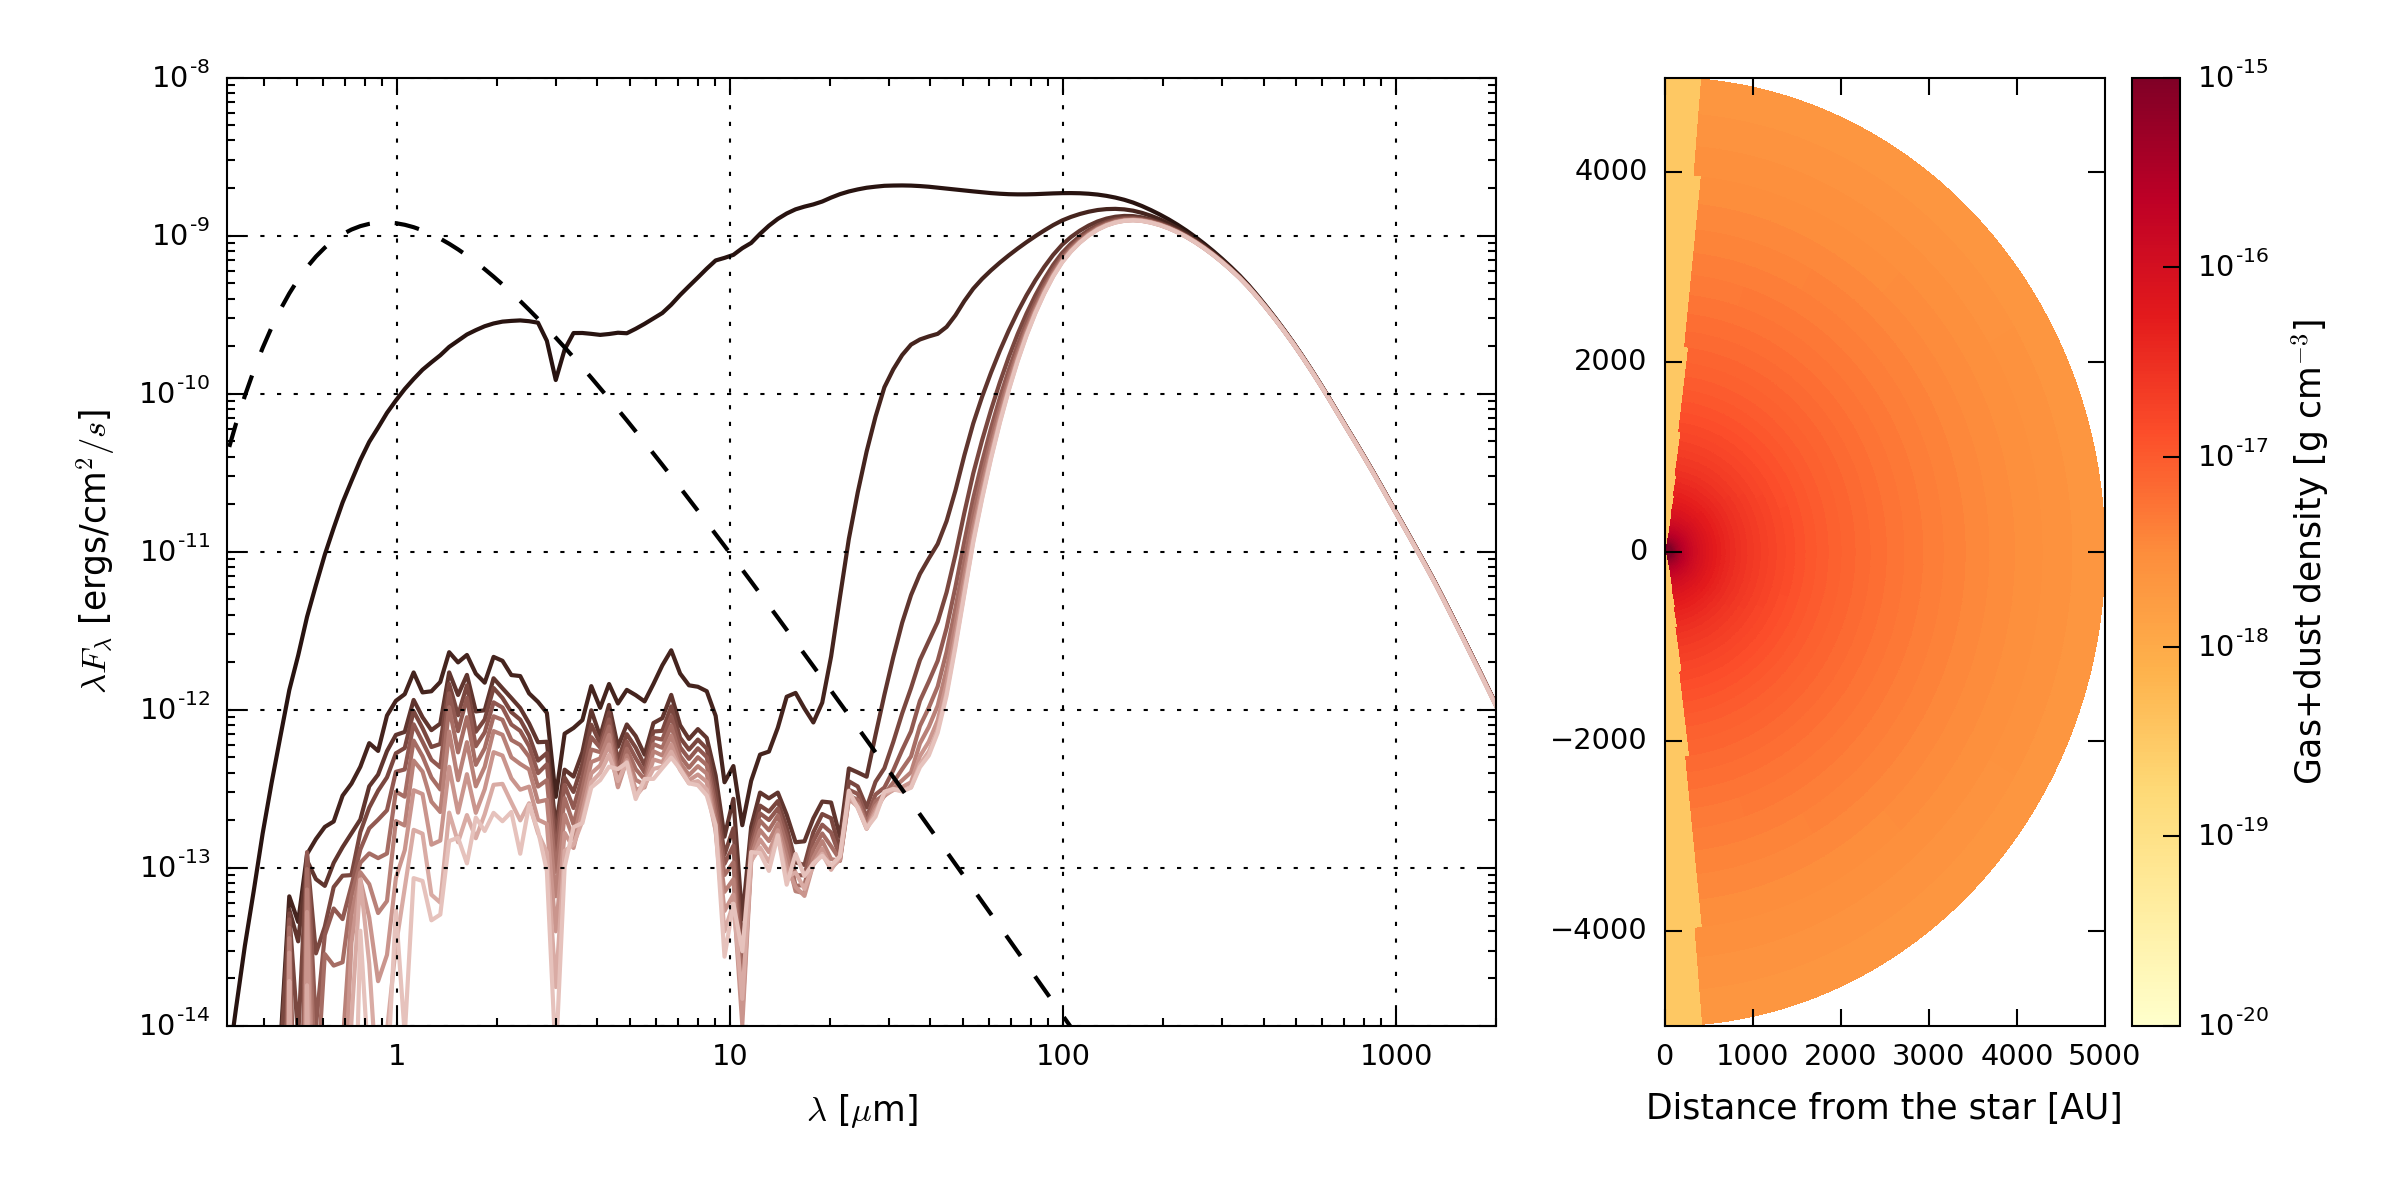
\includegraphics[width=\textwidth]{Figures/test_whitney_class0_nice.png} 
} \par\medskip
\subcaptionbox{Stage I.\label{subfig:StageI}}{
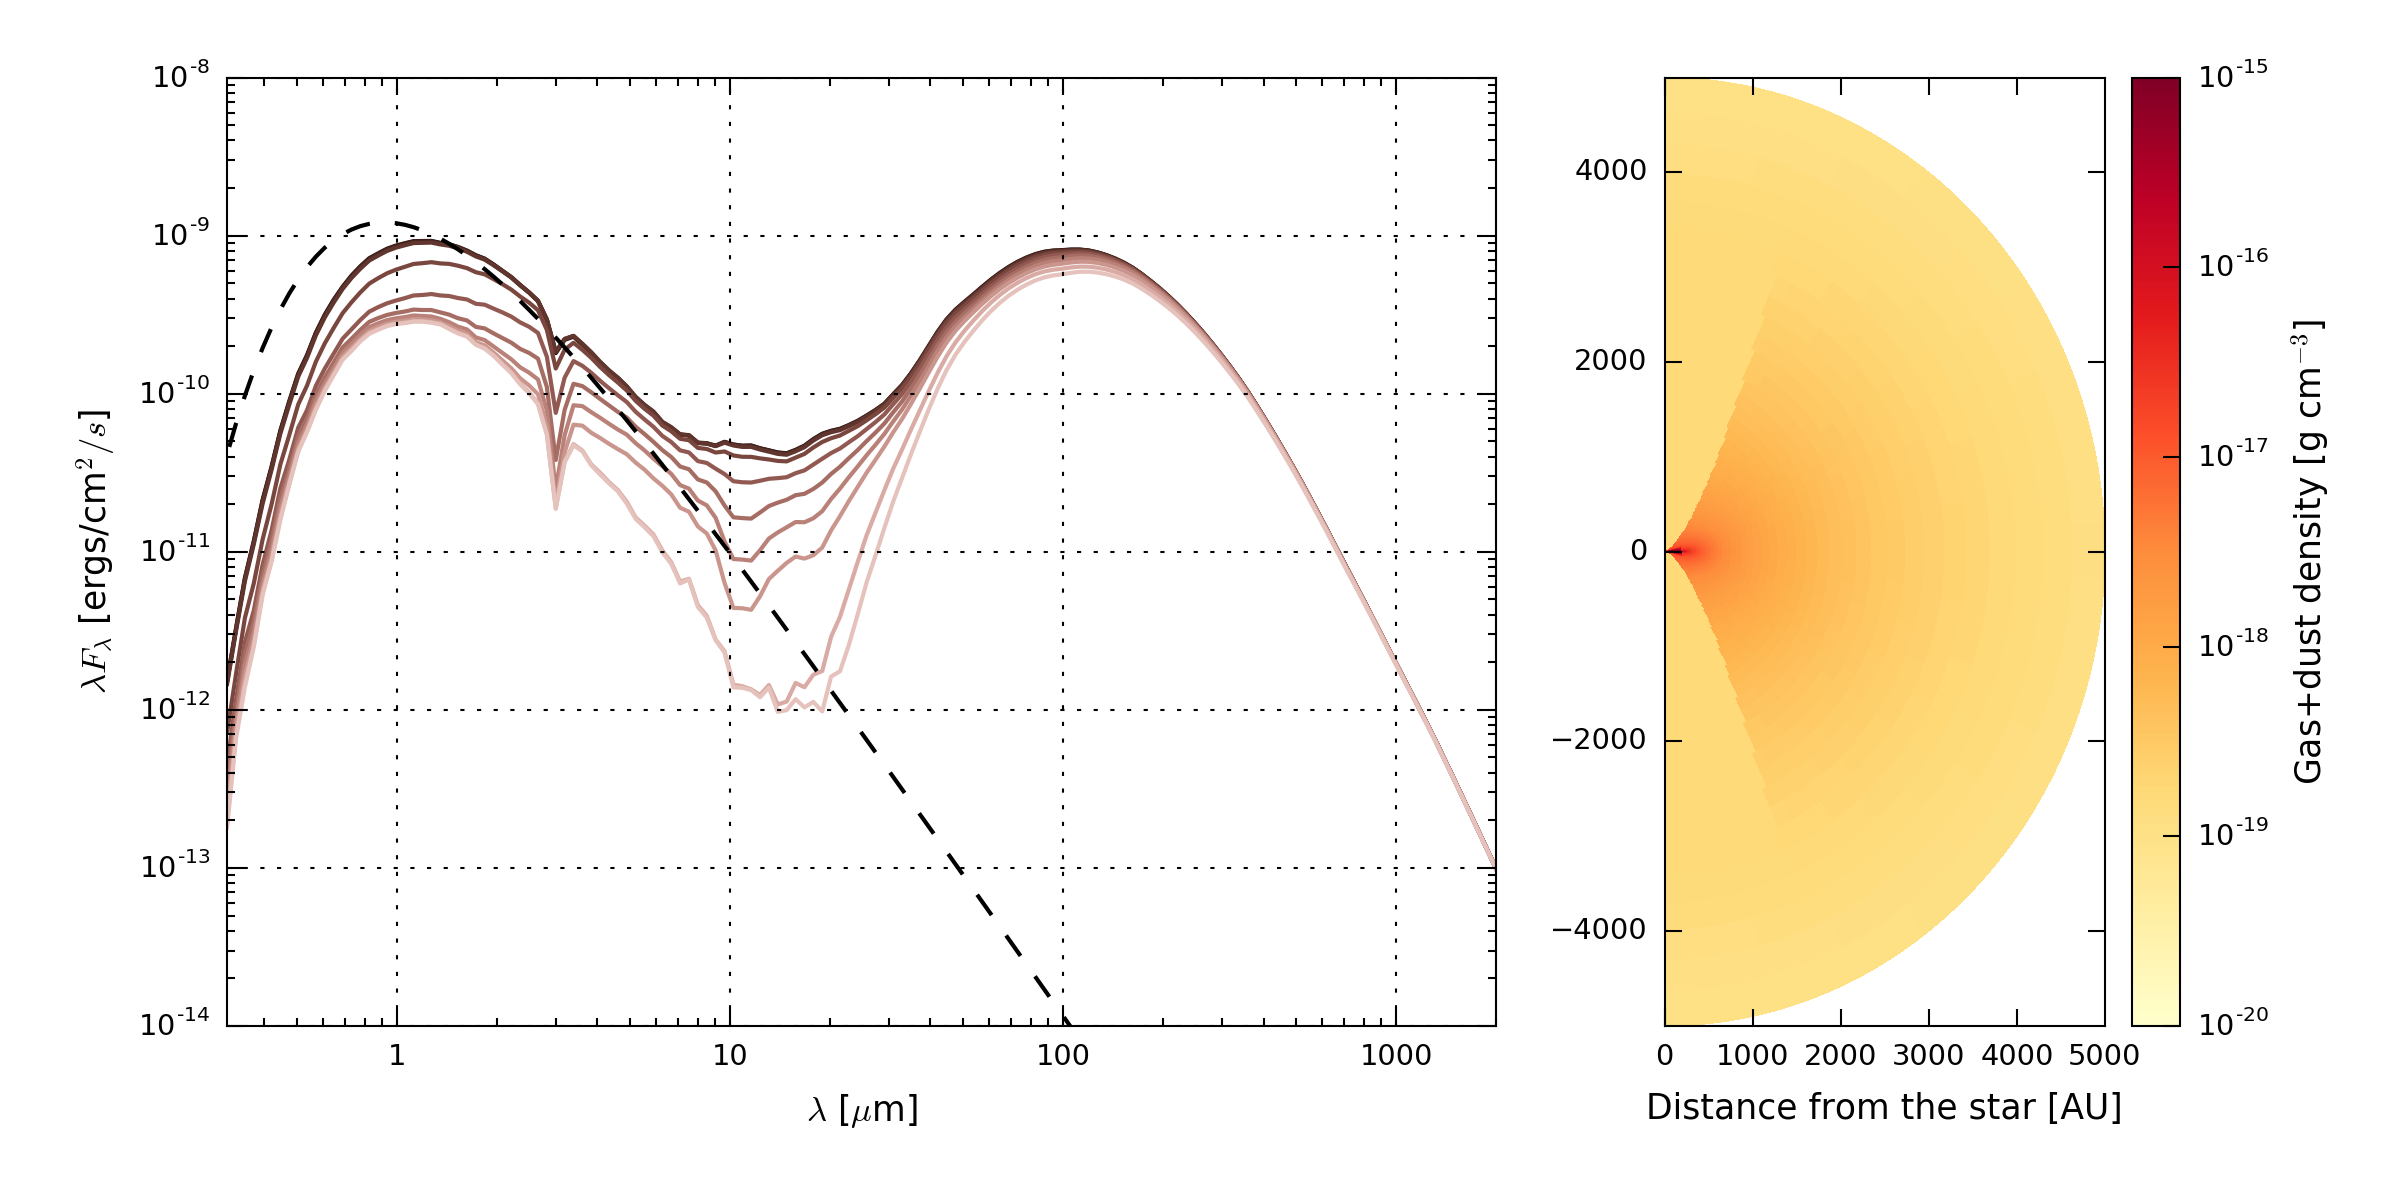
\includegraphics[width=\textwidth]{Figures/test_whitney_classI_nice.png} 
} 
\caption[Early evolution of YSOs]{Early evolution of YSOs.}
\label{fig:EarlyStages}
\end{center}
\end{figure}

\begin{figure}
\begin{center}

\subcaptionbox{Stage II.\label{subfig:StageII}}{
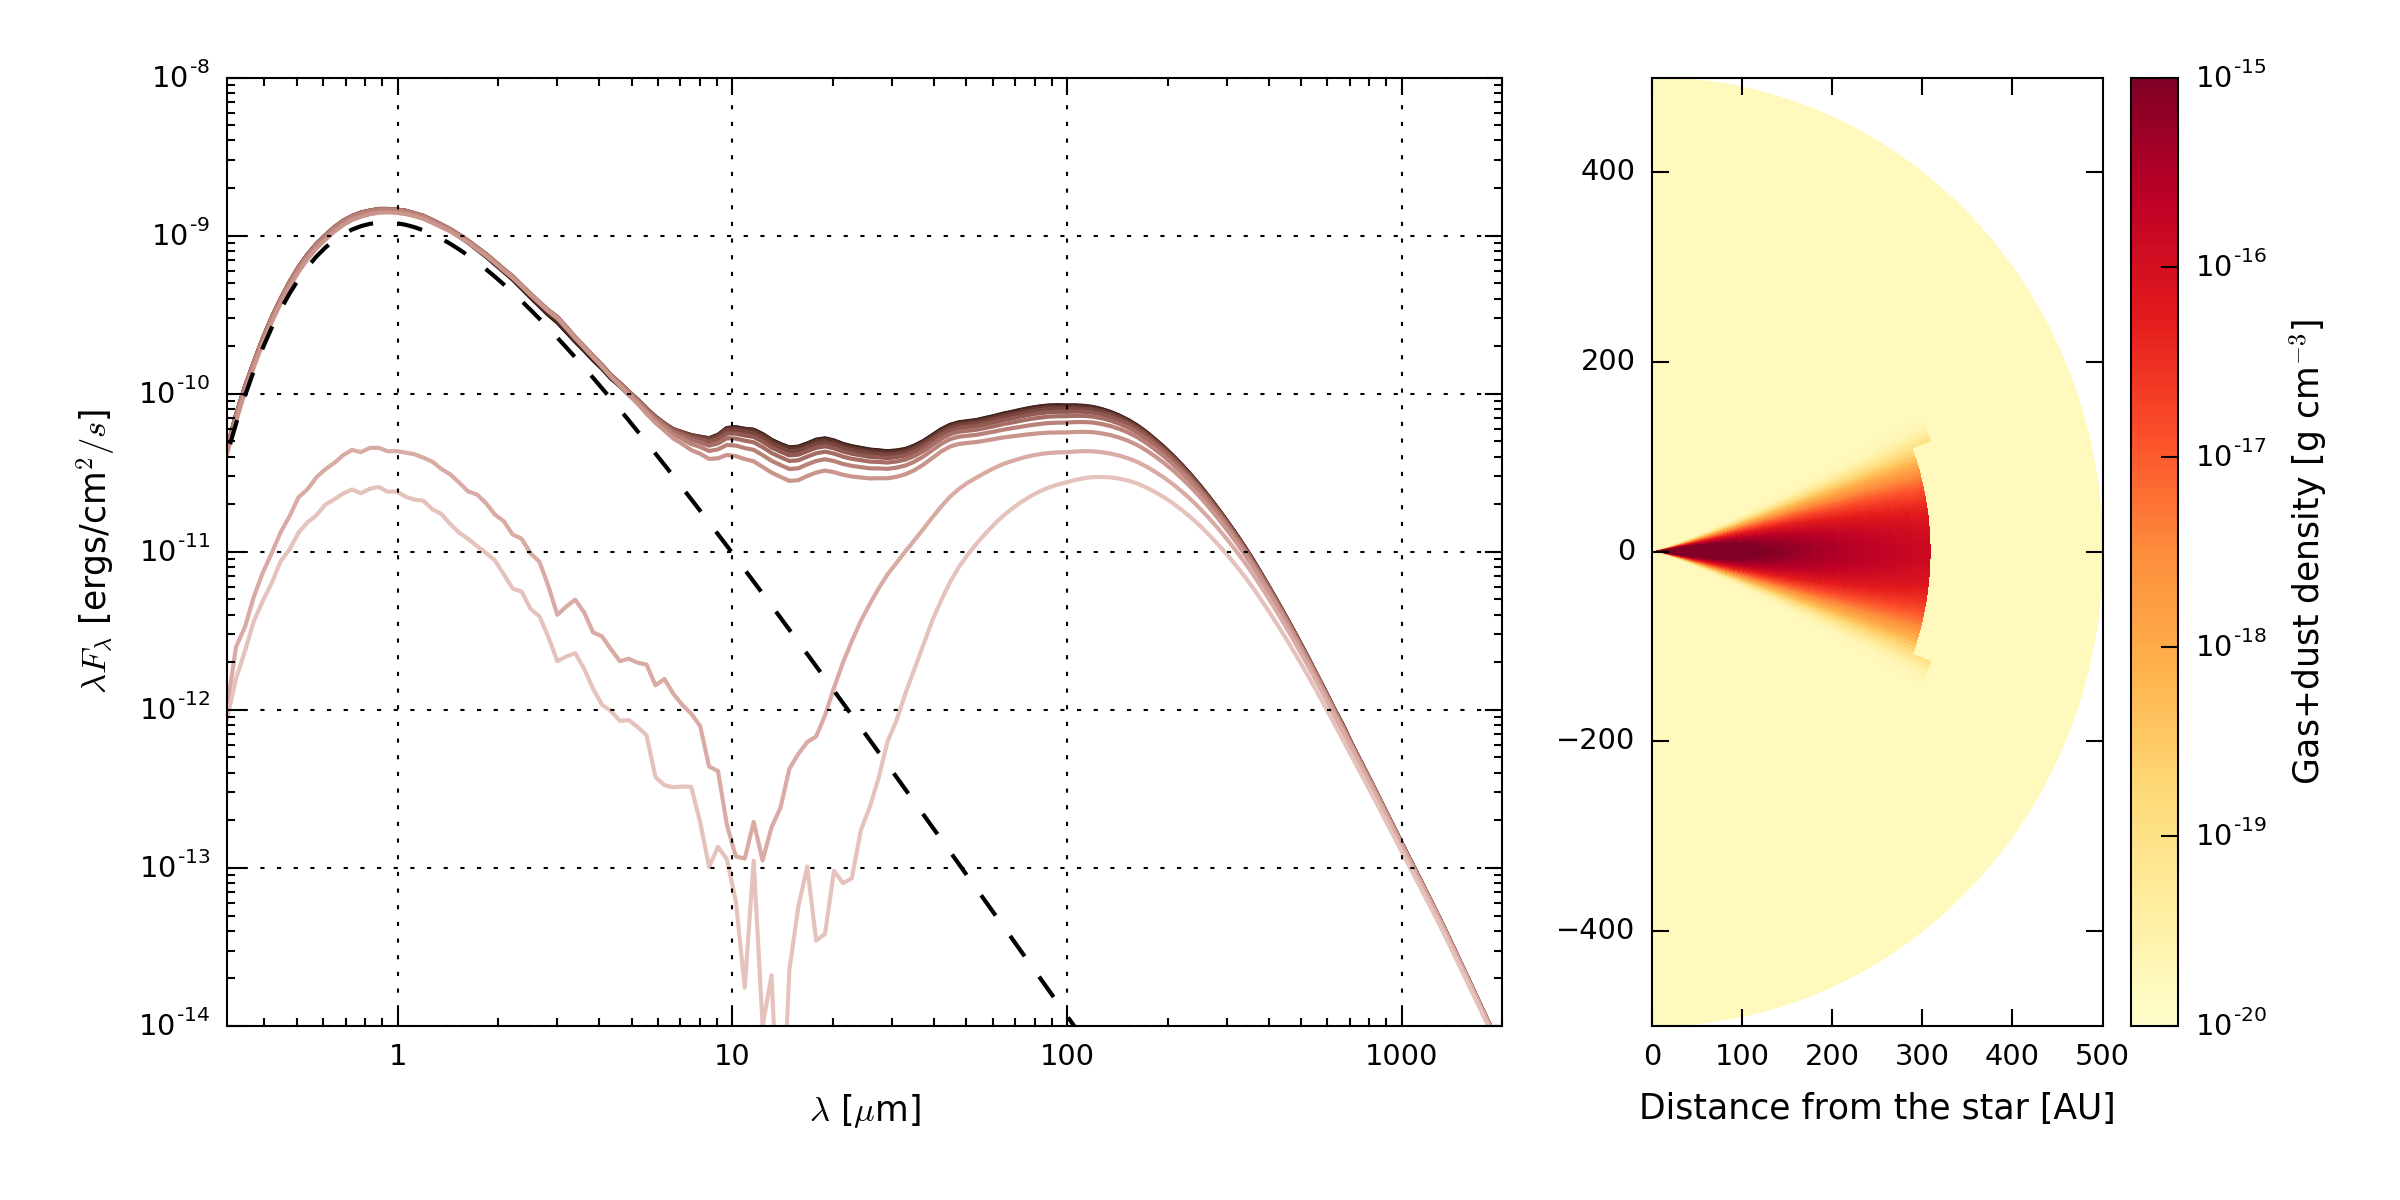
\includegraphics[width=\textwidth]{Figures/test_whitney_classII_nice.png} 
} \par\medskip
\subcaptionbox{Stage III.\label{subfig:StageIII}}{
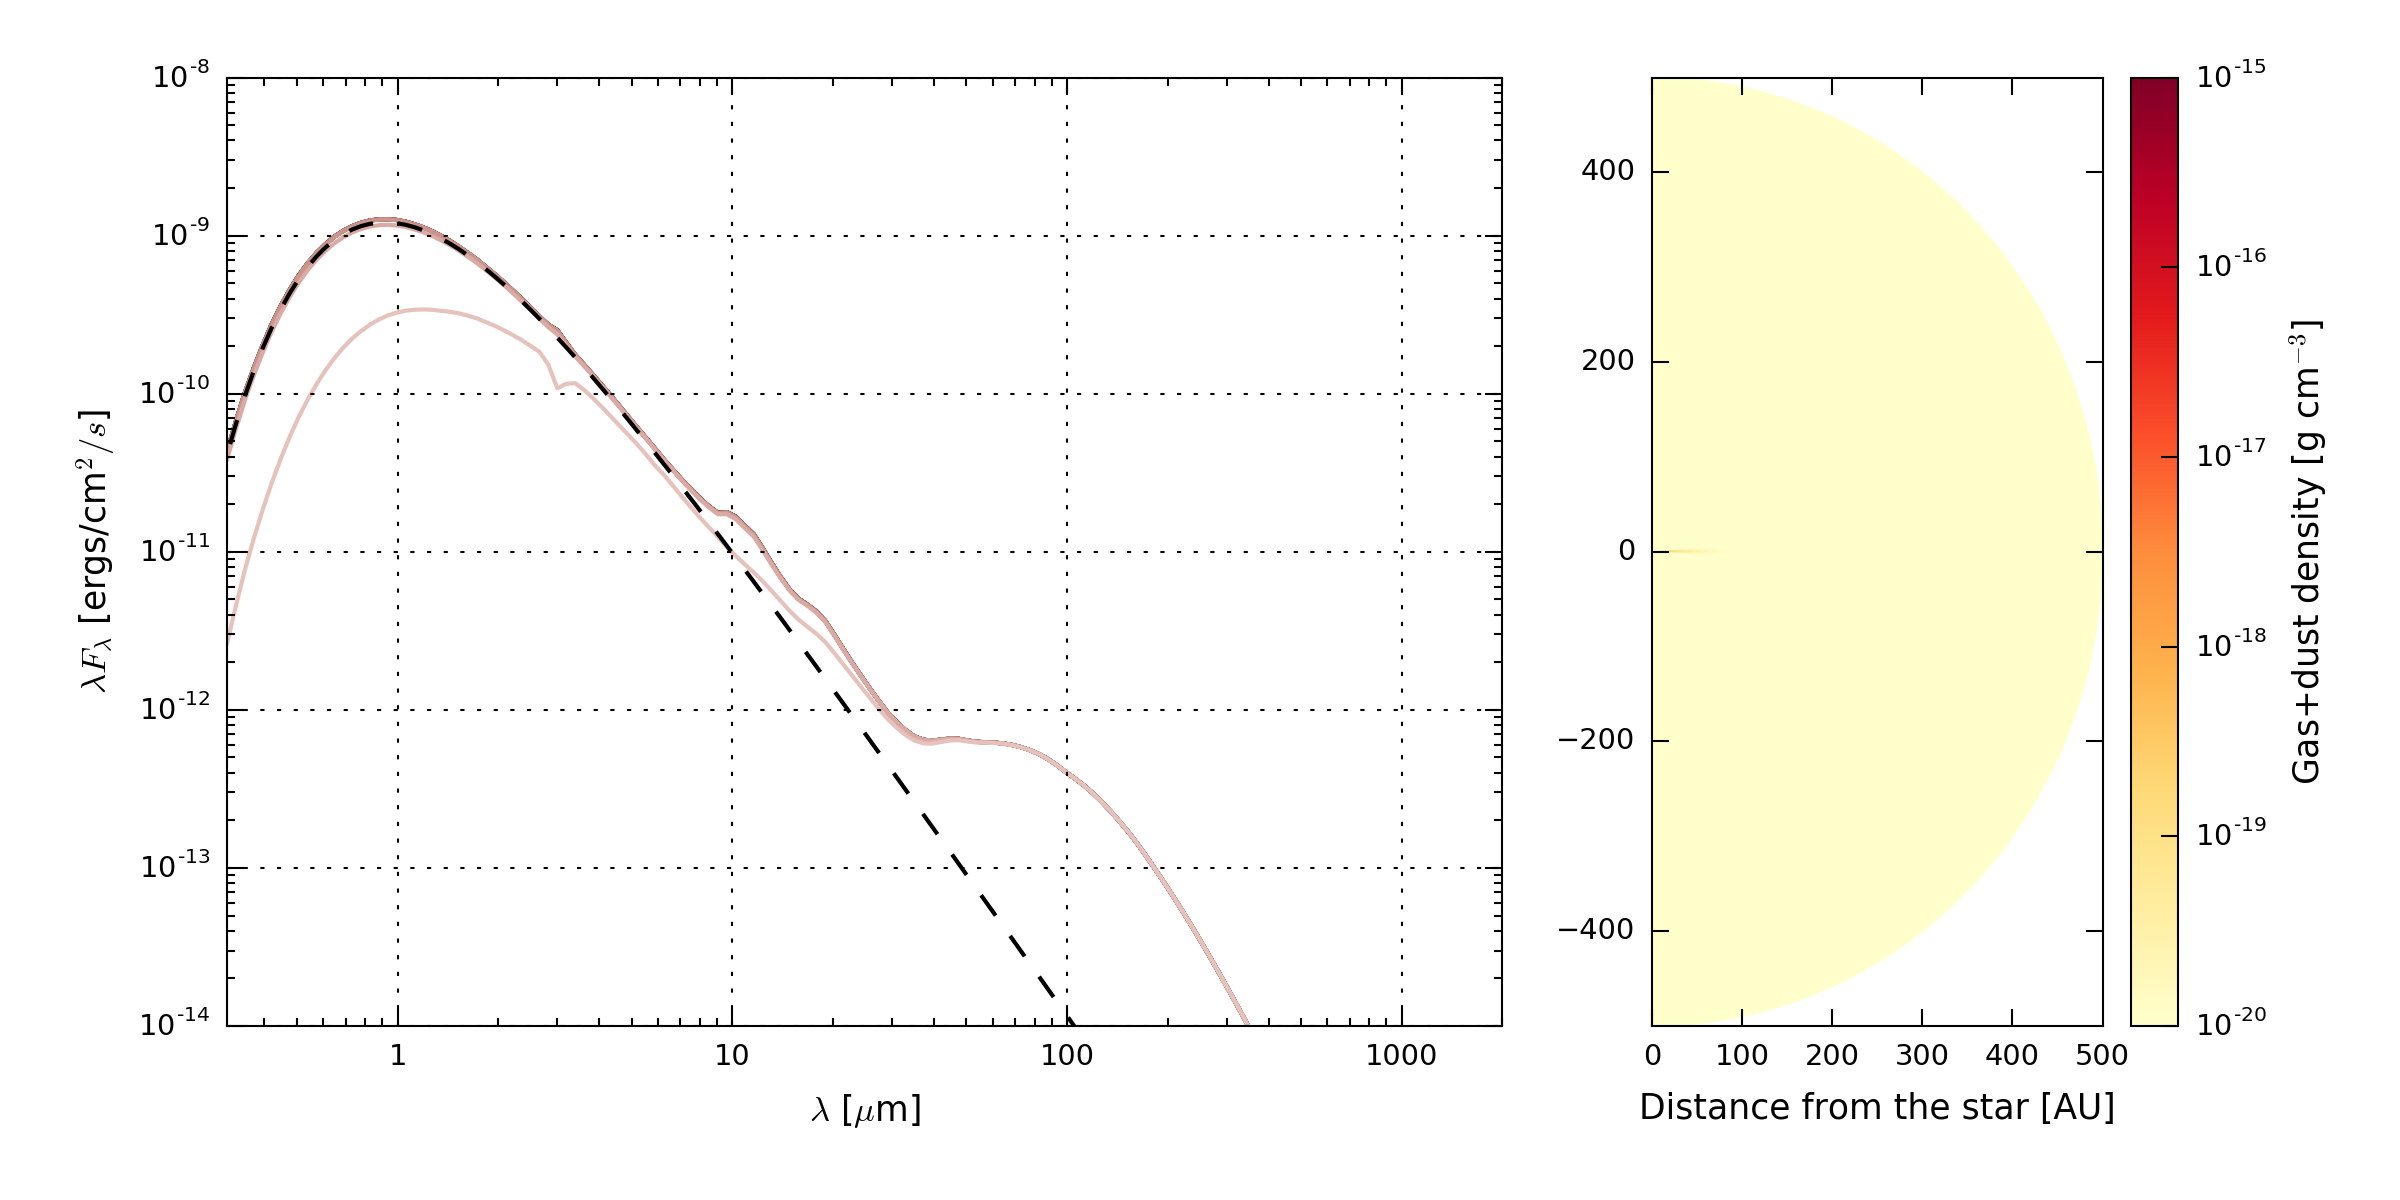
\includegraphics[width=\textwidth]{Figures/test_whitney_classIII_nice.png} 
}
\caption[Late evolution of YSOs]{Late evolution of YSOs.}
\label{fig:LateStages}
\end{center}
\end{figure}


\begin{itemize}
\item Class 0: Most the of short-wavelength ($<\SI{10}{\micro\meter}$) light is highly obscured by the dust in the massive envelope. Most of the emission is around \SI{100}{\micro\meter} and into the submillimeter/radio regimes. If there is a disk, it is very small. Some authors \citep{Dunham:2010bx} classify a source as Class 0 as long as the amount of the mass in the envelope is at least half the total mass.
\item Class I: Light scatters at short wavelength off the dust grains to give us a hint at the embedded object, but it still very obscured. The envelope's mass is lower, and the disk extends to larger distances. The typical spectral index $\alpha$ is positive.
\item Class II: The YSO is now a pre-main sequence star, with a spectral index $-1.5 < \alpha < 0$ a significant circumstellar disk. This is traditionally referred to as a classical T-Tauri star.
\item Class III: Still a pre-main sequence star, but most of the accretion has stopped, and $\alpha < -1.5$. The envelope has almost completely disappeared, and so has most of the disk.
\end{itemize}

An illustration of canonical spectral energy distributions (SED) and density structure is shown in Figs.~\ref{fig:EarlyStages,fig:LateStages} for the four main stages, with parameters taken in \citet{Whitney:2003kc}. On the left of each picture, the SED is the measurable quantity when the YSO is unresolved at all wavelengths. The challenge is to estimate the density structure (to the right) by measuring the SED. The different lines plotted in the SEDs are different inclination angles, highlighting the enormous impact of the viewing angle on the potential interpretation of these SEDs. The dashed line corresponds to the Planck function from the central source. These models were run using the Hyperion software \citep{Robitaille:2011fc} with "OH5" dust \citep{Ossenkopf:1994tq}, as discussed in more details in Section~\ref{subsec:dust}.

These SEDs are often characterized and classified with standard observational metrics, such as the bolometric temperature and luminosities \citep{Myers:1993en,Dunham:2010bx}:

\begin{align}
\Lbol &= 4\pi d^2\int_0^\infty\Snu d\nu,\\
\Tbol &= \num{1.25e-11} \frac{\int_0^\infty \nu\Snu d\nu}{\int_0^\infty \Snu d\nu}~\si{\kelvin},
\end{align}
%
where \Snu is the flux density in \si{\watt\per\raiseto{2}\meter\per\hertz}. 

\subsection{Mass accretion in clusters}


The discussion in the previous section represents a canonical view of how a single core collapses and forms a star. While it is convenient to assume that the original core forms a fixed reservoir of gas that will determine the star's final mass, it is likely too simplistic, since these YSOs are preferentially forming inside of clusters close to multiple other YSOs and sharing a dense, often turbulent environment \citep{Porras:2003kxa,Allen:2007wqa,Gutermuth:2009gca}. 

%Approximately 60\% of all stars are thought to form in clusters with 100 or more stars (\cite{Porras:2003p1395}; \cite{Allen:2007p1439}). These $>$100 star clusters have characteristic sizes of 2-4 parsecs with peak surface densities of 100-1,000 stars per square parsec and a typical median distance between nearest neighbor young stellar objects (YSOs) of 0.03 to 0.06 parsecs \citep{Gutermuth:2009p1325}.

The question of how stars acquire their final mass is key in studying star formation. Does dense gas fragment into isolated centers of collapse? Do young stars competitively accrete material from a surrounding common reservoir? Do gravitational interactions between forming young objects play a significant role in setting the final stellar mass function? Better observational understanding of these clusters is necessary to address these questions and to discriminate between the different models, as noted by \cite{Bonnell:2006ee}, \cite{Offner:2011ex} and \cite{Myers:2011fy}.

Given the typical stellar separations in clusters with fully formed young stellar objects and the typical densities of gas in these cores, \num{1000}'s of astronomical units (\si{\au}, \SI{1}{\parsec} = \SI{206265}{\au} - are the size scales over which forming stars must draw material to become 0.5-10 solar masses. Once the material is inside \SI{100}{\au}, it is strongly bound to the forming stellar system (which may be one or more stars) and its fate is determined. To give an idea of the possibilities for accreting material, Fig. \ref{fig:SFscenarios} sketches three scenarios for how stars could capture mass in the cluster environment: core collapse, competitive accretion, and collisional merging. In core collapse (CC) \citep[Fig.~\ref{scenarios:a},][]{McKee:2003gxa, Myers:2011fy}, the cluster's gas fragments into cores which collapse individually to form single, binary, or small multiple star systems; the available mass is defined by the original fragment. In competitive accretion (CA) \citep[Fig.~\ref{scenarios:b},][]{Bonnell:1997vta}, the initial core collapses but contains a small fraction of the star's final mass; additional mass is captured competitively with other forming stars from the surrounding dense core gas. In collisional merging (CM) \citep[Fig.~\ref{scenarios:c},][]{Bonnell:2002et}, the initial fragments interact gravitationally and form larger mass cores before and during the formation process. 

Are all these processes observed at once in star forming clusters? What conditions favor one versus the other, and why? Are these processes observed at different stages in the cluster's history?

Recent studies by \cite{Offner:2011ex} and \cite{Myers:2011p1338} compared protostar luminosity distributions with predictions of models based on these ideas. \cite{Offner:2011ex} suggest that both CC and CA could work if the star formation rate in the cluster increases with time; \citep{Myers:2011fy} finds that a CA-type model with additional Bondi accretion to produce massive stars works best. As highlighted at the end of the \cite{Offner:2011ex} paper, larger cluster samples and better data on massive stars are needed to improve the observational constraints on models.


%\paragraph{The Initial and Core Mass Functions}
%Initial mass function across multiple locations \citep{Myers:2014ct}: The IMF has similar properties of shape, mass scale, and high-mass slope among field stars, open clusters, and young clusters (Kroupa 2002, Chabrier 2005, Bastian et al. 2010).
%
%In the most widely-discussed explanation, an IMF distribution of masses arises as a cluster-forming clump fragments into condensations, or cores, due to self-gravity and turbulence. In such turbulent fragmentation models, the mass distribution of cores (CMF) is a mass-shifted version of the IMF (Padoan \& Nordlund 2002, Hennebelle \& Chabrier 2008, Hennebelle \& Chabrier 2009, Hopkins 2012), matching observational studies of cores in nearby star-forming regions (Motte et al. 1998, Alves et al. 2007, Konyves et al. 2010)
%
%\citep{Myers:2014ct} has all I need here to describe the IMF and CMF
%
%Describe the various theories of SF in clusters. 



\begin{figure}[ht!]
\begin{center}
\begin{subfigure}[b]{0.3\textwidth}
\centering
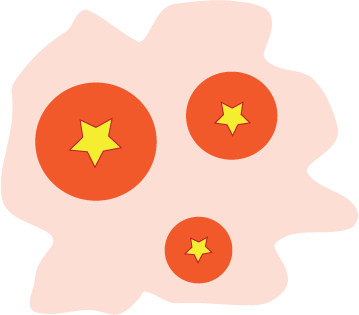
\includegraphics[width=0.98\textwidth]{Figures/CC.png} 
\caption{}
\label{subfig:scenarios:a}
\end{subfigure}
\begin{subfigure}[b]{0.3\textwidth}
\centering
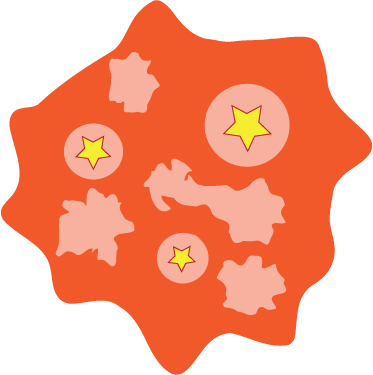
\includegraphics[width=0.98\textwidth]{Figures/CA.png} 
\caption{}
\label{subfig:scenarios:b}
\end{subfigure}
\begin{subfigure}[b]{0.3\textwidth}
\centering
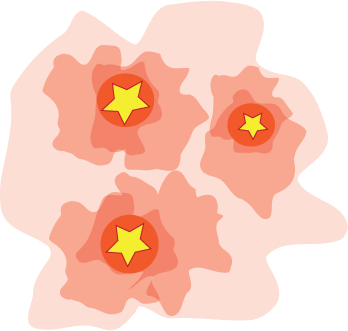
\includegraphics[width=0.98\textwidth]{Figures/Coalescence.png} 
\caption{}
\label{subfig:scenarios:c}
\end{subfigure}
\caption[Scenarios of clustered star formation]{Three scenarios of clustered star formation. Darker colors indicate higher densities.}
\label{fig:SFscenarios}
\end{center}
\end{figure}



%\subsubsection{Outstanding scientific questions}
%Examples: \citep{Hennebelle:2012dk} \citep{Kennicutt:2012ey}
%Ex: WHERE DO THE INEFFICIENCIES COME FROM?
%
%Luminosity problem \citep{McKee:2007bd}
%Angular momentum problem and magnetic flux problem  \citep{McKee:2007bd}
%How the mass-to-flux ratio increases so dramatically during star formation is one of the classic problems of star formation (Mestel \& Spitzer 1956). 

\section{Dust as a tracer of star formation}
\label{subsec:dust}

Despite being a small component by mass, interstellar dust is an important component of galaxies. Dust grains are heated up by absorbing the short wavelength emission from stars and re-radiate in the thermal infrared, accounting for $\sim 30\%$ of the total luminosity of the galaxy \citep{Mathis:1990jk}. 

Observationally, dust plays perhaps the most important role when it comes to studying star formation. It usually is assumed that dust is well mixed with the gas, which makes it an excellent tracer of the gravitational well and mass distribution in YSOs. Because H$_2$ and He molecules have very few spectral signatures, they are difficult to observe and study directly. Dust grains block UV and visible star light and emit continuum far-IR radiation, opening a large region of the electromagnetic spectrum for astronomers to study the properties of star formation. Alternative tools to study star formation are dedicated to observing spectral lines of the molecular compounds of the ISM such as CO and other dense gas tracers, a prospect that limits the study to the most dense regions since these compounds typically freeze out onto the surface of dust grains for sufficiently high densities [REF?]%and requires more assumptions to link the abundance of these compounds to the more massive neutral H$_2$ and He gas.


\subsection{Dust populations and properties}


Perhaps the first understanding of the composition of dust grains in the ISM was described by \cite{Mathis:1977hp}, where they studied the absorption spectrum of the diffuse ISM, and found that the measurements were appropriately fitted with a dust grain composition of silicates and small graphite particles \citep{Stecher:1965eq}. They were able to fit the observed extinction curve with canonical grain-size distribution, typically $n(a) \propto a^{-3.5}$, where $a$ is the grain size (assuming spherical grains) and $n(a)$ corresponds to the number of grains of sizes $<a$. This assumes low and high cutoffs for the grain sizes, typically \SI{50}{\angstrom} and \SI{0.25}{\micro\meter}, respectively.

This grain-size distribution model was later on enhanced by \cite{Cardelli:1989dp} to account for the difference in interstellar extinctions (hence size distributions) across different galactic lines of sight. These authors were able to successfully parameterize this size distribution using a single parameter, $R_V$, which is the ratio of the total extinction $A(V)$ to selective extinction\footnote{Extinction and colors are expressed in magnitudes} (or color) $E(B-V) = A(B) - A(V)$. Smooth distributions of sizes of graphite and silicate grains between the less dense regions of the ISM, where $R_V = 3.1$, and the dense clusters, where $R_V = 5.3$ \citep{Kim:1994iu}. 

Observations in the thermal infrared from space telescopes have detected strong absorption lines at \SI{9.7}{\micro\meter} and \SI{18}{\micro\meter} which are attributed to stretching mode of Si-O and bending mode of O-Si-O, confirming the presence of silicates in dust compositions \citep{Weingartner:2001du}. Other emission features at 3.3, 6.2, 7.7, 8.6, and \SI{11.3}{\micro\meter} \citep{Sellgren:1994vz} were attributed to bending and stretching modes of polycyclic aromatic hydrocarbons \citep[PAH, see][]{Gillett:1973bh,Allamandola:1985cf}, which are complex, planar organic molecules.
 
A consolidated model matching all-sky measurements by instruments on the COBE space observatory confirms the composition of amorphous silicates and carbonaceous grains with sizes ranging from large grains ($\approx\SI{1}{\micro\meter}$) down to tens of atoms \citep{Li:2001gk}, where the larger carbonaceous grains have graphitic properties and the smaller population have PAH-like properties.


[Molecular hydrogen is believed to form by recombination on the surface of dust grains [hollenbach and salpeter 1971, and are only able to survive from UV photodissociation within these obscured clouds.]




Knowing the dust composition and size distribution of grains is important to properly predict its observational behavior and relate it to the physical quantities of interest, since the goal of the exercise is to use dust as a tracer of star-forming mechanisms. A given dust model needs to provide several key quantities that can be used in radiative transfer modeling (see Section~\ref{subsubsec:radiative}), such as the albedo, the scattering function, and the opacity.

In the very cold regions surrounding a YSO, where the dust temperature typically never exceeds a few tens of \si{\kelvin}, it is expected that these dust grains are covered by a mantel of ices which can dramatically change their radiative properties, especially at short wavelengths. 

\subsection{Basics of dust extinction}

Dust grains are responsible for the extinction within molecular clouds, inside of clusters, and also within each YSO; although these various extinctions could originate in different types of grain populations. The typical representation of this extinction uses the ratio of observed over expected flux, measured in V-band: $\Av \equiv A(V) = 2.5\log(\Fnu^\textrm{obs}/\Fnu)$. The extinction, $A(\lambda)$, is a function of wavelength and is expressed in magnitudes. An alternative representation is to consider the extinction as being caused by an optical depth $\tau_\ext$ such as $\exp(-\tau_\ext) = \Fnu^\textrm{obs}/\Fnu$. We have the equivalence $A(\lambda) = \num{1.086}\tau_\ext(\lambda)$.

At sufficiently long wavelength, dust opacity models can usually be represented by a simple power-law, $\Knu = \kappa_0(\nu/\nu_0)^\beta$, with the index $\beta$ depending on the specifics of the dust model. The opacity $\Knu$ is expressed in \si{\raiseto{2}\centi\meter\per\gram}, and can be interpreted as a extinction cross-section per unit mass. Most dust models assume a 1:100 dust-to-gas ratio, and derive opacities per unit {gas+dust} mass, instead of just dust mass. From a radiative transfer perspective, the observed specific intensity from a thermal source $\Bnu(T)$ in the optically thin regime is $I_\nu = \tau_\nu \Bnu(T)$, where the optical depth is $\tau_\nu = \Knu\int{\rho_\dust dl}$. $\rho$ is the density and the integral is calculated along the line of sight to the source. %Note that the optical depth can also be expressed in terms of the extinction cross-section \Cext~as $\Knu = \Cext(\nu) / m_\dust$, where $m_\dust$ corresponds to the mass of a dust grain.

A measure of the intensity from a source can thus lead to an approximation of the total mass within a primary beam, for a given dust grain model. For a source with a measured sub-millimeter flux density $S_\nu$, in the optically thin regime we can write $S_\nu=\tau_\nu\Bnu(T)\Omega$, where $\Omega$ is the solid angle of the source, $\Omega = A/d^2$, with $A$ the area of the source and $d$ its distance. We obtain a measure of the mass by writing $M\approx A\int{\rho dl}$, to obtain \citep{Shirley:2000gh}:
\begin{equation}
M = \frac{S_\nu d^2}{B_\nu(T_\dust)\Knu},
\end{equation}
with a dust temperature is usually taken to be between 10 to \SI{20}{\kelvin}. 

With only near- to far-IR wavelengths observations, however, it is more difficult to estimate the dust mass, because the system is usually not in the optically thin regime and very dependent on the local geometry and viewing angle. To use these observations, which are interesting because they naturally are at higher resolution than single-dish submillimeter data, detailed radiative transfer models are usually required (Section~\ref{subsubsec:radiative}).


Dust grains can either scatter or absorb photons, and both of these processes have their own frequency-dependent efficiency. Large grains are usually considered in local thermal equilibrium (LTE), in which case the thermal emission balances out the absorption. However, small grains ($<\SI{50}{\angstrom}$) can be subject to stochastic heating, where single photons can heat up the grains to much higher temperatures for very short amounts ot time. Scattering mechanisms can be much more complicated to represent, as they usually involve a scattering phase function, describing the deflection angle of incident photons (which also depends on wavelength). Most models show that dust grains are preferentially forward-scattering [CITE Draine?]. The scattering properties of the dust model exclusively influence the short-wavelength emission, while the absorption properties influence all wavelengths. 

%Talk about dust properties in the galaxy: \citep{Collaboration:2014dz} Using
%Also maybe mention papers by Dale etc DIRBE/COBE
%
%A large number of dust models exist (see Section~\ref{subsubsec:radiative})
%
%In clusters and cores, it is likely that grains are covered with a layer of ice which could dramatically influence their radiative transfer properties

\subsection{Radiative transfer modeling}
\label{subsubsec:radiative}

Several radiative transfer codes exist in the literature, and we have explored a few of them. We opted for a recently-developed package called Hyperion \citep{Robitaille:2011fc}, which is a Python interface to a 3D Monte-Carlo code by \citet{Whitney:2013cw}. The code is versatile, parallelized, can accept different dust models and can generate various types of geometries and density grids.

Hyperion functions in two steps. After choosing a discrete grid to represent a density model and adding energy sources, the temperature structure of the dust is calculated by propagating photon packets and determining the dust LTE temperature in each cell. Multiple iterations of this process are usually required to converge to a decent thermal structure.

Once the dust temperature is known, the dust becomes a source of thermal radiation. This type of radiation is modeled using ray tracing, which provides a very good signal-to-noise ratio (\SNR). The light from the central source which was not absorbed, however, needs to be propagated and scattered off the dust grains, for example using a method called peeling-off \citep{YusefZadeh:1984ff}. For non-isotropic scattering, this process has relatively low \SNR, hence requires a lot of photons packets to function properly. While there are future plans to implement raytracing for scattering \citep{Robitaille:2011fc}, we are currently forced to wait long times for simulating YSOs with massive envelopes because of this problem.

[Put models of YSOs with different masses here.]

These models usually present a large amount of degeneracies, especially when the entire range of wavelengths is not covered, as it is the case for most astronomical sources. For example, an SED will look very different depending on the viewing angle. If we see down the throat of the cavity, the short-wavelength light from the central source will not exhibit a lot of extinction. If we observe this same source through the disk and envelope, these same wavelengths will show a lot of extinction. The short wavelength, up to the peak of the SED, are very geometry-dependent and highly degenerate parameters.

This realization helped us target our work using this code. Others \citep[e.g][]{Robitaille:2006cb} have produced standardized grids of pre-computed models which randomly sample a very large number of source geometry parameters. These grids are routinely used by the community to fit a set of unresolved SED measurements at discrete wavelengths. However, most often the scatter in the parameters for the few best fit models prevents from drawing meaningful conclusions on the observations. 

[Example?]
%For example, in a Class 0 or I YSO, the disk geometry and mass has a very insignificant impact on the resulting SED. [Put a model of the SED with and without disk?]

One of the key challenges of using this code is to determine which dust models to use. For this work, we choose to use exclusively OH5 dust \citep{Ossenkopf:1994tq}, which represents grains with an ice mantle which are the result of a coagulation phase of an initial distribution of grain sizes following $n\propto a^{-3/2}$. This model was found to accurately represent some grain distribution in the ISM [NEED CITATION, CHECK OUT TRACY'S PAPER].

\subsection{Observing star formation}

In the past decade, space-based infrared observatories such as \Spitzer\ and \Herschel\ have really allowed the beginning of the detailed study of dust around forming stars, by sampling the SEDs in key spectral regions, such as the PAH region (with the IRAC instrument on \Spitzer), the mid-infrared (with the MIPS instrument, especially its \SI{24}{\micro\meter} channel), and the far-IR (with the PACS instrument on \Herschel). 

However, these observatories lack the required angular resolution to observe the key physics of star formation in dense clusters in the key wavelength region between \SI{30}{\micro\meter} and \SI{200}{\micro\meter}. For a diffraction-limited single aperture telescope, the angular resolution and spatial resolutions $R_\theta$ and $R_\textrm{linear}$ are:
\begin{align}
R_\theta &= \ang{;;17.6}\left(\frac{\lambda}{\SI{70}{\micro\meter}}\right)\left(\frac{D}{\SI{1}{\meter}}\right)^{-1}, \\
R_\textrm{linear} &= \SI{0.04}{\parsec}\left(\frac{d}{\SI{500}{\parsec}}\right)\left(\frac{\lambda}{\SI{70}{\micro\meter}}\right)\left(\frac{D}{\SI{1}{\meter}}\right)^{-1},
\end{align}
which shows that even with \Herschel and its \SI{3.5}{\meter} primary mirror and its \SI{70}{\micro\meter} channel, we can barely resolve clustered YSOs (typical separations of a few hundredths of \si{\parsec}), let alone study their structure in detail. 

To further complicate the problem, most space observatories are tailored for very sensitive observations, so the brightest regions of clusters often cause saturation issues due to a lack of dynamic range. These two issues have continually prevented us from gathering a good picture of the physics in these dense and important regions of stellar birth.

[Image that shows the saturation/lack of resolution]

[Talk about SOFIA]
%\subsubsection{Observing facilities}
%
%Introduction notes: [DELETE THIS]
%\begin{itemize}
%\item \citep{Kennicutt:2012ey} Maybe start with a description of the ISM
%\item \citep{Terebey:1984hi} Basics of infall; 
%It is well understood how self-gravity can concentrate gas in the presence of magnetic fields, turbulence, rotation, and thermal pressure, leading to protostar formation and accretion ( McKee \& Ostriker 2007; Adams \& Shu 2007; Ballesteros-Paredes et al. 2007)
%\item \citep{Adams:1987gy} Spectral evolution of young stellar objects; describe classes of stellar objects, using models and make sure to include size scales; YSO vs protostar
%\item Need to mention something about star formation efficiency
%\item Need to mention something about outflows and feedback \citep{Maury:2009co}
%\item \citep{Larson:1994cj} Molecular cloud characteristics; maybe a good start for text | Give definition of cloud (gravitationally bound in the Virial sense), in terms of number of candidates and stellar mass density (Lada 2003)
%\item \citep{Myers:2009fv} It is widely accepted that most stars form in concentrations of dense gas (Beichman et al. 1986), and that such young stars are most frequently found in groups and clusters in molecular clouds (Lada \& Lada 2003). It is less clear how the mass of a protostar is related to the mass of the dense core where it forms.
%In one view, a core is essentially a fixed-mass reservoir of gas, which contributes a significant fraction of its initial mass to its protostar. Then core and protostar masses are proportional, and their mass distributions have the same shape (Motte et al. 1998; Alves et al. 2007). Many authors have suggested ways to form a mass distribution of cores which resembles the IMF, particularly from processes of turbulent fragmentation (Hennebelle \& Chabrier 2008 and references therein).
%In another view, a core is the densest part of a more extended distribution of gas, with no physical barrier to accretion (Shu 1977; Myers \& Fuller 1992; Caselli \& Myers 1995; McKee \& Tan 2003). Protostars originate in cores, but their masses do not correlate (Bonnell et al. 1998; Bate \& Bonnell 2005), or their correlation depends on fragmentation and core definition (Swift \& Williams 2008), or on the range of gas dispersal times (Myers 2008, hereafter Paper 1). Alternately, their correlation may be coincidental rather than genetic (Hatchell \& Fuller 2008).
%\item \citep{McKee:2010iw} Protostellar mass function
%\item \citep{Bonnell:1997vta} Accretion in small clusters
%\item \citep{Evans:1999gz} Review of physical conditions of star formation, also a good place to start
%\item \citep{Myers:2011fy} These results suggest that a simple model is needed for the dense parts of clusters, where protostars start accreting in condensations resembling dense cores, where they can also gain mass from the core environment, where their accretion durations are specified, and where protostar mass is not tied to the gravitational collapse of an isolated initial condensation. | This comparison favors the core–clump model over the isolated core model for star formation in embedded clusters. It suggests that initial core structure need not set protostar mass, and that massive stars are clump-fed.
%\item Clusters are laboratories for studying a wide range of astrophysical phenomena; stars of large range of masses which are formed roughly simultaneously (Lada 2003), can understand stellar evolution theories; 
%\item \citep{Lada:2003il} Cluster formation within molecular clouds: Because a cluster is held together by the mutual gravitational attraction of its individual members, its evolution is determined by Newton's laws of motion and gravity; |
%Stars form in dense gas; therefore, it is not surprising that a high fraction of all stars form in highly localized rich clusters because most of a cloud’s dense gas is contained in its localized massive cores.; |
%This would suggest that there is a direct mapping of clump mass to stellar mass and that the substructure of cluster-forming cores reflects the initial conditions of the star-formation process in dense cores. |
%The structure of an embedded cluster is of great interest since it likely possesses the imprint of the physical process responsible for its creation. In particular, structure in the youngest embedded clusters reflects the underlying structure in the dense molecular gas from which they formed. | A fundamental consequence of the theory of stellar structure and evolution is that, once formed, the subsequent life history of a star is essentially predetermined by one parameter, its birth mass
%\item \citep{Bate:2003cv} Evolution of clusters (dynamics, showing simulations and such); same as \citep{Bonnell:2003iw}; realte to potentially having multiple generations of stars within the same cluster; \citep{Allen:2007wqa}
%\item \citep{Mathis:1990jk} Pioneering paper on the interstellar extinction by dust
%\item \citep{Weingartner:2001du} Paper on dust populations
%\item \citep{Li:2001gk} Very small grain population and non-LTE heating
%\item \citep{Compiegne:2010kk} Large surveys, PAHs, VSG, etc
%\item \citep{Bastian:2010ig} Big picture: importance to universal IMF
%\item \citep{Kennicutt:2012ey} The Challenge of Spatially Resolved Star-Formation Rates in Galaxies
%\item \citep{Hennebelle:2012dk} Observational issues: 
%
%\end{itemize}
%


%How do stars accrete their material in dense, clustered environments? Multiple theories have been put forth to explain the forces at play in these important regions of stellar birth \citep[e.g.][]{Bonnell:1997vta, McKee:2003gxa}. Pivotal differences in the theories center around what drives the parsec-scale dense cloud to form many stars and how the forming stars acquire their mass. Does dense gas fragment into isolated centers of collapse? Are turbulent motions in the gas driving creation of super-critical cores? Do young stars competitively accrete material from a surrounding common reservoir? Do gravitational interactions between forming young objects play a significant role in setting the final stellar mass function? Better observational understanding of these clusters is necessary to address these questions and to discriminate between the different models, as noted by \cite{Bonnell:2006ee}, \cite{Offner:2011ex} and \cite{Myers:2011fy}.
%
%\textbf{The primary goal of the proposed science plan is to understand how stars accrete material on the scales of 100's to 1,000's of AUs in forming cluster cores}. Given the typical stellar separations in clusters with fully formed young stellar objects (YSO) and the typical densities of gas in these cores, 1,000's of AUs are the size scales over which forming stars must draw material to become 0.5-10 solar masses. Once the material is inside 100 AU, it is strongly bound to the forming stellar system (which may be one or more stars) and its fate is determined. To give an idea of the possibilities for accreting material, Fig. \ref{fig:SFscenarios} sketches three scenarios for how stars could capture mass in the cluster environment: core collapse, competitive accretion, and collisional merging. In core collapse \citep[Fig.~\ref{scenarios:a},][]{McKee:2003gxa, Myers:2011fy}, the cluster's gas fragments into cores which collapse individually to form single, binary, or small multiple star systems; the available mass is defined by the original fragment. In competitive accretion \citep[Fig.~\ref{scenarios:b},][]{Bonnell:1997vta}, the initial core collapses but contains a small fraction of the star's final mass; additional mass is captured competitively with other forming stars from the surrounding dense core gas. In collisional merging \citep[Fig.~\ref{scenarios:c},][]{Bonnell:2002et}, the initial fragments interact gravitationally and form larger mass cores before and during the formation process. 
%
%Are all these processes observed at once in star forming clusters? What conditions favor one versus the other, and why? Are these processes observed at different stages in the cluster's history? These questions need more observational data to be answered. \textbf{We propose to gather information about the gravitational potential within the cluster, the distribution of the turbulence, and the gas densities} \citep{Bonnell:2006ee}. This will advance the problem to the next stage and help answer some of these questions.
%


%\subsection{The physics of star formation}
%
%In here, describe the basics of star formation; include state-of-the art dynamical modeling, radiative transfer modeling, SED fitting, etc.
%
%\subsubsection{Dust populations}
%
%About how to estimate the mass
%
%\subsubsection{Geometry and model degeneracies}
%
%\subsubsection{Foreground extinction}
%
%\subsection{Clustered environments}
%
%\subsubsection{Observational challenges}
%
%Surveys vs pointed observations; show why BETTII is important using IRAS20050's example;
%
%\subsubsection{Observing facilities}
%
%Spitzer, Herschel, SOFIA; radio interferometers;


%% Chapter 2

\chapter[Far-IR double-Fourier interferometers and their spectral sensitivity]{Far-infrared double-Fourier interferometers and their spectral sensitivity} % Main chapter title

\label{chap:phasenoisepaper} % For referencing the chapter elsewhere, use \ref{Chapter1} 

%----------------------------------------------------------------------------------------

\section{Introduction}
Observations at mid- to far-infrared wavelengths from the Earth's surface are extremely 
limited by the large atmospheric opacity in this region of the spectrum. Space-based telescopes 
like IRAS \cite[12-100 $\um$;][]{1984ApJ...278L...1N}, ISO \cite[2.5-240 $\um$;][]{1996A&A...315L..27K}, \textit{Spitzer} \cite[3.6-160 $\um$;][]{2004ApJS..154....1W}, AKARI  \cite[1.7-180 $\um$;][]{2007PASJ...59S.369M}, WISE \cite[3.4-22 $\um$;][]{2010AJ....140.1868W} and \textit{Herschel} \cite[55-672 $\um$;][]{2010A&A...518L...1P} have demonstrated the scientific value of observations at 
these wavelengths; but the spatial resolution of space-based observatories is limited by the cost 
and complexity of building and flying progressively larger aperture telescopes. 
Interferometry is a common solution to this problem on the ground, and is a viable path forward to obtain much
higher resolution than what single apertures can provide. 
In particular, spatio-spectral interferometry \citep{Mariotti:1988vea} is a way to achieve 
high angular and spectral resolutions at far-IR wavelengths from above the atmosphere, without the cost and limitations of large single apertures. 

Several space-based interferometer concepts, the Far Infrared Interferometer \citep[FIRI;][]{2009ExA....23..245H}, the Space Infrared Interferometer Telescope
\citep[SPIRIT;][]{Leisawitz:2007if}, and the Submillimeter Probe of the Evolution of Cosmic Structure \citep[SPECS;][]{Harwit:2006hl}, have been proposed and use spatio-spectral interferometry to achieve the much needed angular resolution to 
study astronomical processes such as the birth of stars and planetary systems, the activity in 
galactic nuclei and the formation of galaxies in the distant universe. The FIRI and SPIRIT concepts have
two mirrors which are movable on one axis along a monolithic truss to provide a range of baseline lengths.
%the angle of the baselines is changed by rolling the spacecraft about the line of sight to the desired target. 
SPECS consists of three spacecraft connected via tether to achieve baselines of order 1~km. 

There are numerous engineering challenges to be addressed before such missions can become reality. A number of them can be tackled with testbeds \citep[e.g.][]{Leisawitz:2012ik, 2012ApOpt..51.2202G} and small-scale pathfinder missions. These missions 
will likely be two-element, single baseline interferometers in space or on balloon platforms,
such as the Balloon Experimental Twin Telescopes for Infrared Interferometry \cite[BETTII;][]{2014PASP..126..660R} and to a certain extent the Far-Infrared Interferometric Telescope Experiment \cite[FITE;][]{2010TrSpT...7.Tm47K}.  
These pathfinders will have very limited baseline coverage and
rather than producing full images, they will focus on reconstructing 
spectral information from closely-spaced sources. This paper explores
aspects of the noise in spectral measurements specific to these instruments.

\subsection{Spatio-spectral interferometry}

In their pioneering paper, \cite{Mariotti:1988vea} lay out the principles of spatio-spectral 
(or double-Fourier) interferometry. A spatio-spectral interferometer consists of a Fourier transform 
spectrometer (FTS), where a delay line mechanism modulates the optical path difference (OPD) between two independent light beams before combining them in the pupil plane. The instrument produces interferograms, which are arrays of power measurements as a function of the OPD. Unlike traditional FTS, 
where a single incoming beam is split, delay-modulated, and recombined, a double-Fourier 
interferometer utilizes multiple light collectors pointing to the same astronomical source and 
combines the incoming light from the collectors pairwise in the pupil plane. The orientation 
and magnitude of the baselines - the vectors between each pair of light collectors - determines 
which  spatial frequency of the astronomical image the instrument measures. 
Longer baselines correspond to higher angular resolutions. The ``double-Fourier" aspect comes from 
the fact that the interferogram measured on a given baseline is related to the Fourier Transform (FT)
of the spatial and spectral distribution of the source emission.
Two FTs are used to reconstruct the full spatio-spectral datacube representing the 
astronomical scene: the spectra which are more directly related to the power as a function of time
delay difference between the two incoming beams (equivalent to the OPD) and
the source 2D spatial structure on the sky which is more directly related to measurements
accumulated from many different baseline vectors. The length of the baseline vectors can be changed by modifying the distance between the light collectors. The orientation of the vectors can be changed by rotating the baseline with respect to the source on the sky.
The plane representing the source visibilities
as a function of baseline vector is referred to as the ($u, v$)-plane and is a common notion in ground-based submillimeter and radio interferometry. This paper focuses on the reconstruction of the spectrum from closely-spaced point sources using single-baseline measurements, and does not address the techniques and sensitivities involved in using multiple baseline lengths to produce an image of the scene; a mathematical formalism that covers imaging is already proposed in \cite{Elias:2007jsa}.

%LGM: ZPD dependence within columm for large offset not done

Proposed double-Fourier instruments at far-IR wavelengths distinguish themselves from operating interferometers at sub-millimeter and radio wavelengths in several ways. First, they do not directly measure the phase information. The fundamental measurement is a time series of real-valued power as a delay line modulates the OPD in a controlled sequence (for example a linear ramp). The OPD from the delay line, as well as other OPD contributors in each arm of the instrument, and the external OPD created when the line of sight to a source is not perpendicular to the baseline vector, add up to the total OPD.
In double-Fourier instruments, the OPD can be determined by measuring or estimating the various contributors to the total OPD. For a given detector location along the projected baseline vector, there exists a value of the OPD in the delay line that exactly compensates all other OPD contributors. This delay line position results in a zero net total OPD, and is called the Zero Path Difference (ZPD). At this value of OPD, an incoming plane wave traverses the two beam paths reaching the detector exactly with the same phase, for all wavelengths. ZPD corresponds to the center of an interferogram for that detector location. In the
context of this paper, the phase for a given wavelength $
\phi_\lambda$ is related to the OPD between the beams from each arm when they combine, at the time of a data point measurement: $\phi_\lambda = 2\pi\textrm{OPD}/ \lambda$.
%LGM: rearraged above paragraph to define phase later and keep focus on path difference

% In the context of this paper, the "phase" refers to the total optical delay between the beams from both arms when they are combined, for a given location on the detector array. The total OPD is influenced by the OPD between the arms of the instrument, the OPD introduced by the delay line, and  In double-Fourier instruments, the phase for each point of the interferogram can only be known indirectly by measuring or estimating these three OPD contributors: while the measured signal is an power as a function of delay line OPD, the physical information lie in the measured power as a function of total OPD (or phase). For each detector location along the baseline vector, there exists a value of delay line OPD that will exactly compensate the other OPD contributors, hence making the net OPD zero. This point, called the Zero Path Difference (ZPD), is the center of an interferogram at that detector location. Hence, measuring the location of the center of an interferogram can be used to retrieve the phase for each of the points in the interferogram, provided that other factors stay constant

%It is possible, for example, to accurately estimate the phase for each point of the interferogram if the Phase information is derived from acquired knowledge of the true Zero Path Difference (ZPD, equal optical path length for a target position on the sky).

A second important difference for balloon and space interferometers is that collectors are not fixed
to the Earth. In the case of BETTII and SPIRIT, the collectors are fixed to a truss structure which
is part of the mechanical system for pointing the collectors. Consequently, baseline length
and external OPD, as relevant to an astronomical source, are not independent of pointing errors. The impact of errors in baseline length is modest because the relevant measure is in terms of fractions of the collector diameter. Errors in pointing translate into external OPD as the sine of the error angle times the baseline length, while the relevant measure is the wavelength. This can easily become significant;
for example, a 1" pointing error for an 8~m long baseline corresponds to a $38~\um$ shift in OPD.
%LGM: Added last sentence

Third, bolometer-type detectors, such as being built for BETTII and envisioned for SPIRIT, are
easily, and indeed typically, configured as two-dimensional arrays. With pupil plane combination,
the entire field of view has an interferometric response; hence wide-field interferometry over
multi-pixel arrays is straightforward. Fig.~\ref{fig:widefield} shows this concept and sketches the instrumental
response. For the configuration shown with the detector array columns aligned perpendicular
to the baseline vector, ZPD is the same along lines perpendicular to the baseline vector projected on the detector. As the OPD is swept, it moves across ZPD for the different columns in the array, yielding interferograms with shifted centers corresponding to the changes in external OPD for each source location in the field. 

By sweeping the OPD, the double-Fourier instrument measures interferograms which contain both spectral and spatial information over the detector array. The full spatial and spectral source information can be unambiguously recovered by repeating the delay line sweep over a range of baseline angles and lengths, which correspond to different spatial frequencies on the sky \citep{Mariotti:1988vea}.


\subsection{The case study: BETTII}

The BETTII project \citep{2014PASP..126..660R}, is a motivation for this paper and a near-term application of spatio-spectral interferometry. BETTII consists of two 50~cm siderostats on a fixed 8~m baseline, with a far-IR beam-combining instrument at the center. It will observe the far-IR universe in two 
wavelength bands, 30-50~$\um$ and 60-90~$\um$. The instrument is currently under construction at NASA Goddard Space Flight Center and is scheduled to launch in the Fall of 2016 on a stratospheric balloon from Fort Sumner, New Mexico, to an altitude of 35~km in order to be above most of the atmosphere. For its first flight, BETTII will focus on the study of dense star formation in nearby clusters. While a complete image reconstruction is not possible due to the static baseline length, BETTII will help resolve point source objects that are 0.5-1" apart in the short and long band, respectively, more than ten times the spatial resolution of \textit{Spitzer} at 24~$\um$ and six times the resolution of SOFIA at 37~$\um$.  Combined with a modest spectral resolution of $\R=10 - 50$, BETTII will measure the spectral energy distributions (SEDs) of clustered young stars to determine their evolutionary stage, locate the origin of the far-IR emission, and improve our understanding of how stars accrete their mass in these very dense regions of stellar birth \cite[e.g. see][and references therein]{2014prpl.conf..149T}. For resolved sources, the fixed baseline will not completely lift degeneracies between the spectral and spatial information; however detailed source modeling can put constraints on the distribution of the far-IR emission
\citep[e.g][]{2013ApJS..207...30W}.
%LGM: modified last sentence and added recent reference for modeling.

In this paper, we study how various types of noise propagate to the derived spectrum in an
instrument like BETTII or SPIRIT. In section~\ref{sec:formalism}, we establish a mathematical formalism that can be used to represent interferograms. In section~3, we look at the dominant types of noise in the interferogram and define the relevant timescales associated with spatio-spectral interferometers. In section~4, we derive the spectral signal-to-noise ratio ($\SNR$). In section~5, we apply these results to the special case of BETTII to derive its point source spectral sensitivity.

\section{Mathematical formalism}
\label{sec:formalism}
The general optics layout for a double-Fourier system is shown in Fig.~\ref{fig:optics} for a single baseline. 
The combination of the siderostat and beam compressor acts as an afocal telescope 
which outputs a  parallel beam with a diameter convenient for the rest of the optical train.
The K-mirror in one beam path corrects for the pupil rotation so that the
images of the sky from the two collectors are matched over the field of view.
At the center of the instrument, there are optics for pupil re-imaging, filtering, and beam folding, as required by the specific implementation.
The key components for our purpose are the delay line, beam combiner and detectors. 
The delay line introduces a controlled OPD between both arms.
The two incoming beams are combined in the outputs from the beam combiner. 
We arbitrarily define one output as the ``+" and the other as the \mbox{``-"}. 
To conserve photon energy, the two outputs must be complimentary such that the summed power of the two is
independent of the OPD. In an ideal double-Fourier system, the two beam paths are symmetric about ZPD; 
hence, the power 
from the ``+" and ``-" outputs are equal at ZPD, and have odd symmetry about ZPD. In a traditional FTS at ZPD, one output has fully constructive interference while the other has fully destructive interference, with even symmetry about ZPD.

\subsection{Interferograms for a single baseline}

The interferogram for a single frequency of light measured at the outputs of the ideal double-Fourier instrument can be 
described in terms of the normalized intensity:
\begin{equation}
\hat{I}_\pm(x,\s) = \real(1 \pm i \; \Vb(\s) e^{-2i\pi \s x}),
\label{eq:basicinterferogram}
\end{equation}
where $\s \equiv {1 \over \lambda}$ is the wavenumber of the light in $\cm1$ as per the convention for the FTS literature, $x$ is the instrumental OPD created by the delay line with $x=0$ corresponding to ZPD, and $\Vb(\s)$ is the complex spatial visibility
%LGM: added x=0 statement above
 of the astronomical source for the baseline vector $\baseline$. ``$\real(f)$" indicates the real part of the complex-valued function $f$. The~$\pm$ indicates values for the two output beams: ``+" and ``-" in Fig.~\ref{fig:optics}.
%The "\textit{i}" in the second term of Equation 1 arises because the beam splitter puts a $\pi/2$ phase shift in the reflected beam.  The expression is the real part only because the measured interferogram is real valued. 
The derivation of this expression is given in Appendix~\ref{ap:interfero}.

The normalized complex spatial visibility $\Vb$ has a magnitude of 1 for all baselines for which the source is completely unresolved. For extended sources, the spatial visibility depends on the source geometry, intensity distribution, and the instrument baseline vector as described in Chapter~2 of \cite{2000plbs.conf.....L} 
and Chapter~3 of \cite{Thompson:2008ww}.  
For a normalized source brightness distribution $\hat{\F}$, the spatial visibility with respect to a phase reference position on the sky can be written as:
\begin{equation}
\Vb(\s)  =  \int_\textrm{source} d\Omega \Ahat(\Ds) \hat{\F}(\Ds ) e^{-2i\pi\s\Ds\cdot \baseline},
\label{eq:viseq}
\end{equation}
where $\Ahat$ is the normalized reception pattern of the collecting area; $\baseline$ is the baseline vector between the two collectors and $\Ds$ is the vector on the plane of the sky from the phase reference position to the infinitesimal solid angle $d\Omega$. The resulting visibility as a function of baseline vector is the 2-dimensional FT of the source's sky distribution. 
Since $\hat{\F}$ does not have to be symmetric with respect to the chosen phase center, $\Vb$ is in general complex and can be expressed as an amplitude and a phase, $\Phib(\s)$: $\Vb(\s)  =  |\Vb(\s)|e^{i\Phib(\s)} $.


%, where we are implicitly expressing that
%$\Phib$ is also a function of $\baseline$.

Real instruments have asymmetries, imperfections, and measurement errors which can create phase-shifts between the two optical paths and across the pupils.
% , and differences
%reflection, and transmission properties of optical elements in . 
Fixed instrumental effects 
can be represented by a normalized instrumental visibility loss term, 
$\Vi(\s)$ where the complex quantity $\Vi(\s) = |\Vi(\s)|e^{i\Phii(\s)}$, as described in details in Chapter~3 of \cite{2000plbs.conf.....L}, represents both amplitude losses and phase shifts (see Appendix~\ref{ap:interfero}). Additional phase errors can arise from
imperfect knowledge of the real-time optical path lengths which we will represent as
$e^{i\Phir(\s, x)}$, where $\Phir(\s, x)$ is the ``phase noise"; this term depends on the OPD $x$ through time-dependent phenomena such as mechanical jitters, temperature variations in
the optics support, or pointing errors. In the rest of this paper, we will mostly talk about this ``OPD noise", which is the physical source of the noise, whereas phase noise represents its effects on the interferogram.
The total complex visibility sampled at a single $\s$ by the system is $\Vb(\s)\Vi(\s) e^{i\Phir(\s, x)}$, and it is normalized such that, for an ideal instrument observing a point source, this quantity is equal to 1 at ZPD.

Using Eq. \ref{eq:basicinterferogram} for the monochromatic source, the polychromatic interferogram is the integral over $\s$ of this dimensionless response at each wavenumber. The total amount of power coming into the 2-aperture interferometer within a small wavenumber range $d\s$ is $2\Area \Bspec(\s) c d\s$ where $2\Area$ is the total aperture area in m$^2$, $\Bspec(\s)$ is the spectral flux density in W$\cdot$m$^{-2}\cdot$Hz$^{-1}$ and $c$ is the speed of light in cm$\cdot$s$^{-1}$. 
%LGM: The wavenumber $\s$ has units of cm$^{-1}$ to follow the convention in the FTS literature.
%LGM: added this to the  definition of wavenumbers after Eq 1  
Filters and optics in an instrument cause a wavenumber-dependent transmission profile $\Tbp(\s)$. The quantum efficiency of the detector can depend on wavenumber, $\etaD(\s)$. For multi-pixel detectors the interferogram is measured by matched filtering a point-spread function on a pixel array, which has some efficiency $\etamf$.% Optical elements such as filters and beam splitters/combiners can cause $\s$-dependent phase shifts. 

%Since optical elements along the two light paths are not perfectly
%identical, the source flux density, as seen at the detector, is modified by an instrument transmission function which
%can be complex:
%\begin{equation}
%T_{\inst}(\s) \equiv \etamf\etaD\Tbp \Vi = |T_{\inst}(\s)|e^{i\Phi_{\inst}(\s)},
%\end{equation}
%where all of the terms can be functions of $\s$.

The actual power measured by the instrument can be represented as:
%I_\pm(x) = \real\left(\A \int_0^{+\infty} T_{\inst} \B \left(1\pm i\; \Vb e^{i\Phir(\s, x)} e^{-2i\pi \s x}\right)cd\s \right),
\begin{equation}
I_\pm(x) = \Area c\int_0^{+\infty} \etamf\etaD\Tbp \Bspec \times
 \quad  \real \left[\left(1\pm i \Vi\Vb e^{i\Phir} e^{-2i\pi \s x}\right) \right]d\s,
\end{equation}
where the factor of 2 for the two apertures is dropped because it is implicit in Eq. \ref{eq:basicinterferogram}. All quantities within the integral can be functions of wavenumber, and all the instrumental phase and interferometric loss terms are in $\Vi$ and $e^{i\Phir}$.

Instead of considering each separate output, we use $\I = \I_+ - \I_-$ as our interferogram expression, which cancels out the constant term. We also introduce an interferometric instrument transmission function, which can be complex, which represents the normalized amplitude and phase of the interferogram for a point source of uniform spectrum and no phase noise:
\begin{equation}
T_{\inst}(\s) \equiv \Area c\etamf\etaD\Tbp \Vi = |T_{\inst}(\s)|e^{i\Phi_{\inst}(\s)},
\end{equation}

 We can then write the modulated signal as:
%I(x) = \real\left( 2 \A\int_{0}^{+\infty} i |T_{\inst}| \B \Vb e^{i\Phir(\s, x) + i\Phi_{\inst}(\s)} e^{-2i\pi \s x}cd\s \right).
\begin{equation}
I(x) = \real\left( 2\int_{0}^{+\infty} i |T_{\inst}| \Bspec \Vb e^{i\Phir + i\Phi_{\inst}} e^{-2i\pi \s x}d\s \right),
\label{eq:modsignal}
\end{equation}
where $\Bspec$ is real and $\Vb$ can be complex.

Eq.~\ref{eq:modsignal} can be turned into a Fourier transform by mirroring all quantities to negative wavenumbers. This
convention is explained in detail in \citet{Davis:2001tr} for FTS instruments; the odd symmetry of the interferogram for a system with one beam combiner
and the complex instrumental transfer function means that the incident spectrum on the detectors
must be mirrored to -$\s$ as the negative of the complex conjugate of +$\s$: 
$\S_e(\s) \equiv [T_{\inst} \Bspec \Vb]_e(\s) = {1 \over 2}\left[T_{\inst}(\s) \Bspec(\s) \Vb(\s) - T^*_{\inst}(-\s) \Bspec(-\s) \Vb^*(-\s)\right]$. 
We use the subscript $e$ to denote the reflected function, and will apply this convention in the rest of this paper; this reflection ensures that the integrals keep the same value when are expressed from $-\infty$ to $+\infty$, and does not affect the $\SNR$ estimates: although the signal appears to be divided by a factor of two, so is the noise, as it is spread between positive and negative frequencies.
The interferogram expression is then:
%\begin{equation}
%I(x) = \real\left( 2 \A\int_{-\infty}^{+\infty} i [T_{\inst} \B \Vb]_e  e^{-2i\pi \s x + i\Phir(\s, x)} c d\s \right).
%\end{equation}
\begin{equation}
I(x) = \real\left( \int_{-\infty}^{+\infty} i \S_e  e^{-2i\pi \s x + i\Phir} d\s \right).%\end{equation}
\label{eq:interfero2}
\end{equation}
%[CHANGE THIS TO: INCLUDE THE SINC FUNCTION WITHIN THE INTEGRAL AND DIVIDE IT UP LATER IN THE BANDPASS PROFILE]
\subsection{Measured interferograms}

In practice, the interferogram data are discrete measurements of a real-valued signal on the detectors. Like for most FTS instruments, each data point on the interferogram corresponds to an integration of the detector while the delay line is continually in motion. This decreases the amplitude of the interferogram due to the local smearing of the fringes, but it can be kept to low values by increasing the fringe sampling.
% For example, for constant delay line velocity $v$, a delay distance $\Dx=v\Dt$ is swept during an integration time $\Dt$. 
At each delay $\xn$, the interferogram has a measured value $\Ixn = \frac{1}{\Dx}\int_{\xn-\Dx/2}^{\xn+\Dx/2}\I(x)dx$. To first order, this has the effect of multiplying the power at each wavenumber by $\sinc(\pi\s\Dx)$. For the purpose of this paper, we consider this term to be included as part of the instrumental transmission $T_{\inst}$. Note that the value of the optical delay $\xn$ is the path difference from ZPD, not the physical location of the delay line, since there could be a multiplying factor between the two due to beam folding (e.g., for BETTII, a motion of 1~mm of the delay line creates 4~mm of OPD).
%LGM: Added "the path difference from ZPD" above
%The final, real-valued interferogram can be represented as:
%\begin{equation}
%\Ixn = Real(\A\times \intinf \eta \Tbp\Be\left|\Vb\Vi\right|\sin(2\pi\s\xn + \Phi)d\s,
%\label{eq:finvis}
%\end{equation}
%where $\Phi = \Phib+\Phii+\Phir$ is the sum of the phases corresponding to the source visibility, instrumental, and phase-delay  terms. The measured quantity $\Ixn$ has units of power. 

%\subsection{Fourier transform spectroscopy}
%\label{sec:FTS}

%For a source that is spatially unresolved for all wavenumbers in the bandpass ($\Vb(\s)=1$), the true source spectrum $\Be$ is recovered by Fourier transform of the interferogram with respect to the delay $x$. This is mathematically valid since we made the spectrum of the source symmetric using $\Be$ instead of $\B$, as described in \cite{Davis:2001tr}; this allows us to transform back and forth between the interferogram and the spectrum.

A discrete Fourier transform (DFT) is used to transform a discrete interferogram of $N$ measurements into a complex discrete spectrum with $N$ points. The resolving power of the instrument, $\R = \lambda / \D \lambda$, is dependent on the physical length scanned by the delay line $L$: $\R = L \s / 2 $ for a scan with symmetric length on both sides of ZPD. For these instruments where we scan through the whole interferogram, the data should be
sampled at least at the Nyquist rate for the interferogram response frequency of $\Dx = \lambda/2$. For a sampling exactly equal to Nyquist, we have the relationship: $N = 4 \R$.

For a double-Fourier instrument, as shown in Fig.~\ref{fig:widefield}, the ZPD for different columns on the array occurs at different delay positions $x_{\col}$, related to
the projected baseline length. The simplest way to express this is in terms of the angular offset on the sky of each column, $\xi$, along the
direction of the baseline, $\baseline$:
\begin{equation}
x_{\col} = | \baseline | \sin\xi \approx | \baseline | \xi = 48.7 \um \left({| \baseline | \over 10~\textrm{m}}\right) \ \left( {\xi \over 1~\textrm{arcsec}}\right) ,
\label{eq:delay}
\end{equation}
where we have filled in
practical units for an infrared instrument. For a far-IR interferometer working at $50~\um$, with
1-2~m diameter collectors, the delay shift across the collector point spread function (collector angular resolution) is several to ten wavelengths.
%LGM: Added PSF above to clarify the this is refering to the resolution of the collector
Hence the scan length to cover a wide-field array detector is comparable to the scan length required to achieve
$\R$'s of 100's to 1000's. This property is an important consideration for observation and data analysis strategies.
%With $x_0 = 0$ defined as the center of the interferogram, we can write:
%\begin{equation}
%\DFT(\Ixn) =\sum_{n=-N/2}^{N/2-1}\Ixn e^{2i\pi n k/N}.
%\end{equation}

The ideal interferogram for a point source from a perfect instrument is an odd function of the OPD $x$, so its DFT is purely imaginary. The noise in the interferogram will be converted into spectral noise in both the real and imaginary axes so the real axis is a proportional measure of the noise. 
Referring back to Eq.~\ref{eq:interfero2}, phase shifts caused by the instrumental transfer function and source spatial visibility will
break the anti-symmetry; in practice, the DFT of a measured interferogram is complex and the real and imaginary parts are of interest.
The scientifically interesting quantities are the source spectrum and source spatial visibility: $\B$ and $\Vb$; the fixed
instrumental terms have to be calibrated or properly modeled
by observing a bright point source of known spectrum. The techniques for calibrating FTS systems are well developed
\citep[e.g.][]{Davis:2001tr}, and there are many methods proposed to correct some phase and amplitude errors \citep[e.g.][]{Forman:1966wx, Sromovsky:2003in}. 

The phase noise term $\Phir(x,\s)$ in Eq.~\ref{eq:interfero2}, and the $\SNR$ in the measured interferogram can have significant
impact on the ability to recover the source spectrum with a real instrument. The upper panel in Fig.~\ref{fig:interfero} shows an example of an interferogram (left), and the transformed $\S_e(\s_k)$ (right) for a source with flat power spectrum, multiplied by a flat bandpass function with smoothed edges.
 The middle panel of Fig.~\ref{fig:interfero} shows
the same source and instrument parameters as the upper panel, now with an assumed Gaussian OPD noise of standard deviation equal to 10\% of the central wavelength of the band $\lambda_0\equiv {1\over\s_0}$ (\textit{i.e.}, there is a $\lambda_0/10$ OPD uncertainty for each data point in the interferogram). The lower panel is the top panel observed with a incoherent background noise corresponding to $\SNR=10$ at the peak of the interferogram, and no phase noise. 
The next sections of this paper will analyze these noise contributions and quantify their impact on the derived spectrum.

\section{Noise sources}
The two primary types of noise in a double-Fourier instrument are intensity and OPD noise. The intensity
noise consists of the astronomical and thermal background noise, the photon noise from the source, and the detector noise. The OPD noise arises primarily from uncertainties and changes in OPD, which would prevent us from accurately knowing the $x$-values of measurements in the interferogram before the FT. For convenience, we usually refer to the OPD noise as a percentage of the carrier wavelength. In the rest of this paper, a ``10\% OPD noise" signifies that the OPD for each measurement in the interferogram is known to within an error of 10\% of the carrier wavelength, or 10\% of one full fringe cycle.

\subsection{Intensity noise}
\label{sec:noisesource}
The measured signal has units of power and can be represented as the interferometric signal with additive noise:
\begin{equation}
\Im\pxn = \Ixn + \ni\pxn,
\label{eq:thermalnoise}
\end{equation}
with $\ni$ being the difference of the noise in the two outputs of the interferometer, $\ni = \nA-\nB$. When the beam combiner, optical train, and detectors are symmetric, the residual $\ni$ has zero mean. 
The total noise in $\Im\pxn$, expressed in Noise Equivalent Power, $\NEPtot$, is the sum of the three noise variances: 
\begin{equation}
\NEPtot^2 = 2\NEPph^2 +2\NEPdet^2 +  2\NEPsou^2,
\end{equation}
where $\NEPph$ and $\NEPsou$ are the thermal noise from the background (e.g. sky and warm optics in the case of a far-IR instrument)
and source photon noise, respectively, in one output, and $\NEPdet$ is the noise-equivalent power characterizing each detector's noise (including phonon, readout and Johnson noise). The factor of 2 multiplies each term since we are considering the difference of both outputs.
The relation between $\NEPtot$ and the variance $\varI$ of the noise $\ni$ during an interval $\Dt$ is \citep{Sromovsky:2003in}:
\begin{equation}
\label{eq:sigI}
\varI = \frac{\NEPtot^2}{2\Dt}.
\end{equation}
For space instruments, the noise will likely be dominated by the sky background (zodiacal light, galactic cirrus emission, or optics thermal emission) and detector for a very large fraction of astronomical targets, which tend to be faint; for balloon instruments, emission from
warm optics and the atmosphere sets the noise level in the far-IR.

%There are three dominant sources of thermal photons at balloon float altitude for BETTII: the atmosphere, the dewar window, and the external optics (or telescope). Additional sources, such as the radiation coming from the Cosmic Microwave Background and the zodiacal disk, are much less significant at our observing wavelengths: our estimates show a five orders of magnitude difference. Hence, we will focus on the three main components when working out the noise budget of our instrument. The results are shown in Table \ref{tab:noise}. The values in the table correspond to the background levels per pixel. The sky radiance at float in our bands is taken from \citet{Harries:1980cva}. The radiance from the window and telescope assumes that they are blackbodies at 240~K, with respective emissivities of 0.02 and 0.08. The total optical efficiency assumed for the telescope is 30\%. Combining all these noise sources leads to a background NEP of $1.4\times 10^{-15}$ W.Hz$^{-0.5}$ in band 1 and $6.4\times 10^{-16}$ W.Hz$^{-0.5}$ in band 2. The detector NEP is expected to be less than $3\times 10^{-16}$ W.Hz$^{-0.5}$ in band 1 and $3\times 10^{-16}$ W.Hz$^{-0.5}$ in band 2.

\subsection{OPD noise}
\label{subsec:phnoise}
Observing from the ground at optical wavelengths with a double-Fourier interferometer is limited by the phase coherence 
between the apertures, which is related to the atmospheric coherence time, as discussed by \cite{Mariotti:1988vea}. The short coherence time forces fast scan rates, which degrades the sensitivity of the instrument due to short integration times and phase shifts between sequential scans. 
This is not a problem for flying platforms, since even at balloon altitudes the atmospheric coherence is not a significant 
issue \citep{Rizzo:2012jp}. The major concerns for balloon and space missions are overall instrumental stability, knowledge of ZPD, and pointing errors, which can all contribute to OPD noise.

OPD noise arises in an interferogram when the OPD at the time of a measurement is uncertain, hence compromising the reconstruction of the true $x$-value. Since this uncertainty is a physical delay $\delta_x$, 
the error in phase is wavenumber dependent: $2\pi\delta_x\s$. $\delta_x$ is the difference between the estimated $x$
and the true $x$.
% LGM: Added the sentence above.
% LGM I deleted the "_k$ on the wavenumber because this is not a discrete spectrum statement.
For single-beam FTS instruments, internal laser metrology can provide optical path length 
measurements to high accuracy \citep[e.g.][]{Griffiths:2007uu}, and the separate paths the split beams need to travel can be kept small. 
For double-Fourier instruments, the entire optical paths upstream of the beam combiner affect the OPD, hence it is more challenging to accurately measure and estimate the OPD contributors. 
In addition, common-mode pointing errors of the collectors are directly converted to geometrical delay errors. 
Hence, it is critical to know the position and orientation of the baseline vector with respect to the 
astronomical target with high accuracy in order to properly reconstruct the interferogram.

For this analysis, we identify three timescales that can be used to examine the effects of OPD noise on the interferogram. These timescales are important to consider in the design of the OPD control system of any double-Fourier interferometer. Timescale~1 is the shortest and corresponds to the integration time for a single data point, typically a few milliseconds. In practice, this kind of OPD noise could be created by high-frequency mechanical jitters in the instrument (including the delay line bearing and motor, stiction behaviors and resonant modes, reaction wheels and other self-induced vibrations...). Timescale~2 is the time it takes to acquire one single interferogram over the full field of view and at the desired resolving power, typically on the order of seconds. The sources of noise that can affect this timescale include for example pointing errors and drifts, as well errors in the knowledge of the delay line position relative to
a reference ZPD. Finally, the longest timescale to be considered, timescale~3, is the time it takes to complete one full "track" by co-adding several consecutive interferograms to achieve the desired $\SNR$, typically a few minutes long. During this timescale, it is expected that the change in baseline orientation on the sky does not produce any significant change in the source spatial visibility function. The latter timescale is most importantly influenced by thermal variations and time-varying gradients that could change the optical alignment and mechanical configuration between the two arms. 


%[It is important to realize that while the phase noise can be large during the data acquisition, some can be largely reduced in processing of the data with good models of the noise sources. With this in mind, the following noise derivations apply more on the residual uncertainties on a post-processed data product, rather than in-flight noise control. (PUT THIS SOMEWHERE ELSE?)]

%\subsection{Other sources of noise}

%Talk here about all other sources of noise? What are they actually?

%Our instrument has three relevant timescales for phase noise: 1) the integration time for a single data point (2 to 10~ms), 2) the time that it takes to gather one interferogram ($1-10$~s), and 3) the time over which $M$ interferograms are gathered to complete an observation ($\sim$~10~min). These timescales correspond to high frequency vibrations in the structure, pendulation motion of the instrument package hanging under the balloon, and a combination of pendulation, vertical "bobbing" motion of the balloon, and thermal changes, respectively. BETTII is designed and instrumented to mitigate the amplitude of these effects, but there will be residuals. 

%The interferometric delay $\delaytot$ of an astronomical source consists in the sum of the delays created by the position of the baseline with respect to the source, $\delayext$, and the delays that are internal to the instrument, $\delayint$. External delays change with the pendulum motion of the payload (intermediate timescale), while internal delays will change due to vibrations (short timescale) and thermal variations (long timescale). 

%The magnitude and frequencies of the perturbations for each timescale are difficult to estimate in detail. However, we will make some reasonable assumptions in order to predict sensitivities in the following sections. For the short timescale, the truss and support structure are designed to have lowest vibration modes above 20~Hz where dissipation in the structure will strongly damp oscillations. We expect the phase perturbations to be small over the 1-10~ms timescale. 

%The pendulum modes have been measured before on multiple experiments \cite[e.g.][]{Fixsen:1996kha} and have periods from 2 to 30 seconds and amplitudes up to 10~arcminutes. The highest frequency modes damp faster, especially for an experiment like BETTII that will be staring at inertial targets and not scanning the sky. The gondola pointing control system will compensate for most of these perturbations; we expect to be able to keep the gondola pointed at a given target to within 10-15 arcseconds, once the most powerful modes have damped. The pointing control system is described in detail in \cite{Rizzo:spie2014a}. The residual pointing errors of the gondola will result in external delay errors, and we can expect these errors to be generated at the same frequencies as the perturbations. BETTII will utilize
%measurements from the star camera, the fiber optics gyroscopes, and the tip-tilt pointing corrections to determine these residual errors with an expected accuracy of 1 arcsecond during flight. 
%MAXIME --- IS 1 arcsecond correct??? Put in the correct number.

%A second source of phase error in the intermediate timescale is self-created perturbations in the control loops for the pointing system and the delay lines. These perturbations can be minimized with optimal setting of the gain and bandwidth of the control loops. Post-flight knowledge of the pointing is expected to be accurate to $\sim$0.1~arcsec over a few minutes, and can be held longer when fringes are seen. Knowledge of the error in the commanded position of the delay stages will be measured in real time on BETTII with an accuracy of 0.2~$\um$ with capacitive sensors.

%Finally, thermal distortions are the most difficult to predict. They will depend on the radiative environment during ascent and at float, which is very hard to reproduce in a test environment without using a large vacuum chamber. We expect that the payload will be thermally stable on the order of 10~minutes but it is expected to be systematically cooling throughout most of the flight. 

%The pendulum modes can be very well estimated since they are much slower than any of our sensors (periods of 2~s minimum). Internal vibrations are hard to predict at this point, but they will be predictable we will be able to mitigate them on the ground. Further, they should be minimized by the good symmetry of the payload and our constant effort for synchronous control and command. Finally, thermal distortions are extremely hard to predict. They will depend on the radiative environment at float, which are very hard to reproduce in a test environment without using a large vacuum chamber. We expect that the payload will be stable on the order of 10~min, before a re-calibration of the phase is necessary. 

%\subsection{Important timescales}

%On BETTII, we expect to see three major timescales. The first timescale describes perturbations that occur much faster than the duration of one scan, $\leq 3$~s. We expect to generate most of these perturbations within the payload, from the wheels, the rotation stages, and our other mechanisms, and so they should be predictable. The fastest pendulum modes can be of the order of a scan duration, but these modes damp on the order of a few minutes. The second timescale is between the duration of a scan and the duration of one track. This regime is dominated by the pendulum modes which are on the order of 10-30 seconds. We assume that during one track, there is no significant change in the geometry of the optical train. Finally, the third timescale is beyond the duration of a track, $\geq 10$~minutes. This regime is dominated by thermal changes within the structure, which will inevitably impact the optics and the alignment of the sensors. 



%As discussed in the introduction, errors in pointing of the truss structure result in phase errors. Because BETTII does not have high precision independent metrology of the internal optical paths, errors in knowledge of position of the delay line mirrors also result in phase errors. These two are the main contributors of phase noise on short timescales. On longer timescales, thermal shifts dominate and affect the phase through changes of the structure and the optics caused by asymmetric thermal loads. Hence, two levels of control need to be achieved: a fast control of the relative phase over short timescales for stability; and a slow loop that controls the absolute phase to avoid drifts in ZPD over long timescales. Timescales are discussed in more detail in Section \ref{sec:implications}


\section{Spectral signal-to-noise ratio}
\label{sec:spectralSNR}

\subsection{Effects of Gaussian intensity noise}

%The primary sources of intensity noise in the balloon environment are the photon noise from the incoming light and the detector noise as discussed in Section \ref{sec:noisesource}. Both are expected to have Gaussian distributions.
In the presence of Gaussian intensity noise (thermal background and detector noise), the measured interferogram is of the form of Eq. \ref{eq:thermalnoise}. We suppose that the noise has a variance $\varI$ and zero mean, and is independent of delay position.  In particular, this assumes that the source photon noise is negligible.
The noise in the spectral domain is the transform of the noise in the interferogram domain:
%To determine the SNR in the spectral domain, we start by a Fourier transform of the interferogram:
%\begin{equation}
%\DFT(\Im (\xn) ) = \sum_{n=0}^{N-1}(\Ixn + \ni(\xn)) e^{2i\pi n k/N}.
%\end{equation}
\begin{equation}
\Dx\DFT(\ni) =  \Dx\sum_{n=-N/2}^{N/2-1}\ni(\xn)e^{2i\pi n k/N},
\end{equation}
% WHY IS THERE A DELTA-X RUNNING AROUND HERE WHEN IT WAS NOT PRESENT IN SECTION 3.1
%Half of the noise is in the imaginary domain and half is in the real domain. 
where the $\Dx$ factor is to normalize the noise to a sampling bin \citep{Press:1992vya}, 
and $k$ indexes the $N$ discrete wavenumbers in the spectral domain.
%LGM: Added line above 
The interferogram interval is symmetric with about ZPD (n=0). The noise variance is equal in the imaginary and the real domain, and can be expressed as the variance of the noise transform:
\begin{equation}
\varspec = \Dx^2\VAR\left(\real(\DFT(\ni))\right),
\end{equation}
where $\VAR$ is the variance operation. By writing out the variance we obtain:
\begin{equation}
\varspec = \Dx^2\varI\sum_{n=-N/2}^{N/2-1}\cos^2(2\pi nk/N) =\frac{N}{2}\Dx^2\varI ,
\end{equation}
where we used $\sum_{n=-N/2}^{N/2-1}\cos^2(2\pi nk/N) = N/2$ for $k~\neq~0$. 

The signal at wavenumuber $\s_k$ in the discrete spectrum $\S_e(\s_k)$ is:
\begin{equation}
 \S_e(\s_k) = \frac{1}{\delta\s}\int^{\s_k+\delta\s/2}_{\s_k-\delta\s/2} \S_e(\s)d\s,
\label{eq:signal}
 \end{equation}
where $\delta\s = (N\Dx)^{-1}$. A line of power $P_e$ at $\s_{k_0}$  will thus have an apparent flux density $\S_e(\s_k) = N\D xP_e$ at $k=k_0$ and $0$ for all other $k$. The signal-to-noise ratio in the spectrum can be expressed in general as:
\begin{equation} 
\SNR_k  = \frac{\S_e(\s_k)}{\sigspec} =\sqrt{\frac{2}{N}}\frac{\S_e(\s_k)}{\Dx\sigI} .
\label{eq:spectralSNR}
\end{equation}
Using Eq.~\ref{eq:sigI} and the definition $x_{\textrm{max}}=N\Dx/2$, this becomes:
\begin{equation}
\SNR_k = \frac{\S_e(\s_k)}{x_{\textrm{max}}\NEPtot} \sqrt{N \Dt},
\end{equation}
where $\Dt$ corresponds to the integration time of one data point on the interferogram. As expected the $\SNR$ improves as the square-root of the total integration time, $\sqrt{N \Dt}$, and is adversely affected by increasing NEP and scan length. 
%The signal $\S_e$ in the recovered spectrum is only half the signal of the physical spectrum, because of the definition of $\Be$. 

%The signal in the delay domain is $\I(0) = \dsig\sum_{k}\S(\s_k)=\dsig N\oS$, where $\oS$ is the mean signal in the spectral domain. We also have $\dsig = (N\Dx)^{-1}$, so $\I(0) = \oS/\Dx$ which leads to:
%\begin{equation} 
%\SNR_\mI = \frac{I(max)}{\sigI} = \sqrt{\frac{N}{2}}\frac{\oS}{\sigspec},
%\end{equation}
%and finally:
%\begin{equation} 
%\SNR_\S (\s_k)= \sqrt{\frac{1}{\R}}\frac{\S(\s_k)}{\oS} \SNR_\mI,
%\end{equation}
%where $\R = N/2$ is the spectral resolution of the interferometer. This is the same result as the one derived by \cite{Davis:2001tr} and others. \textcolor{red}{[CHECK IF THERE IS A FACTOR OF 2, WITH SIMULATIONS]}

Defining the central wavenumber of the band as $\s_0$, the spectral resolving power of the transformed interferogram is $\R = \Dx N\s_0/2$. We introduce the sampling parameter $\samp = (\s_0\Dx)^{-1}$ which is the number of data samples per fringe for the central wavenumber in the band. The spectral resolving power at the band center can now be written $\R = \frac{N}{2\samp}$.  In practice one wants to pick a value of $\samp$ that ensures Nyquist sampling on the fringe for all wavenumbers in the band so $\samp \sim 3$ or greater is typically preferred. For a given integration time per data point (given $\SNR_\mI$), increasing the fringe sampling effectively increases the amount of time spent on the fringe, so the spectral $\SNR$ should increase with $\sqrt{\samp}$. Note that as long as we Nyquist-sample the fringe, there is no difference between multiplying the fringe sampling by some factor, and increasing the integration time per data point by the same factor, since in both cases the effective time on the fringe is equally increased.  %Hence, for a constant number of data points in the scan, increasing the sampling comes at a cost of decreasing the spectral resolving power. %Note that $\R$, $\samp$, $N$ and $x_{\textrm{max}$ are not independent parameters. 

It is useful to relate $\SNR_k$ to the $\SNR$ in the interferogram at the location of maximum intensity of the fringe, using physical quantities. The noise in each discrete measurement of the interferogram is $\sigI$. The signal at maximum intensity is $\mI_\textrm{max} = \D\s\oS$, where $\D\s$ is the width of the bandpass filter and $\oS$ is the average value of the signal in the band. Defining $\SNR_\mI = \mI_\textrm{max}/\sigI$, and noting that $\sqrt{N\Dx^2/2} = \frac{1}{\s_0}\sqrt{R/s}$, we obtain:
% PREVIOUS VERSION OF EQUATION
%\begin{equation}
%\SNR_k= \frac{\S(\s_k)}{\oS}\frac{\SNR_\mI}{2\Dx\sqrt{\samp\R}\Delta\s}.
%\label{eq:SNRratio}
%\end{equation}
\begin{equation}
\SNR_k = \frac{\S_e\sqrt{2}}{\sqrt{N}\Dx\sigI} = \frac{\S_e(\s_k)}{\oS}\sqrt{\frac{s}{\R}}\frac{ \s_0}{\D\s} \SNR_\mI .
\label{eq:SNRratio}
\end{equation}
Thus, the $\SNR$ in a channel of the final spectrum depends inversely on the square root of the resolving power $\R$ and the fractional bandwidth $\frac{\D\s}{\s_0}$; and it depends directly on the square root of the number of samples per fringe $\sqrt{\samp}$. 

%For BETTII's short spectral band, $\frac{\Delta\s}{\s_0}$ is in the range of 0.4 to 0.5 and we will be using $\samp=4$. The approximate SNR relationship for BETTII for a flat spectrum source is:  $\SNR_k \approx \frac{2}{\sqrt{\R}} \SNR_\mI$. 
%This result assumes a constant integration time at each point in the interferogram, so each data point has a set $\SNR$.  % and that the interferogram does not extend well beyond the region with coherence. In the latter case, $\SNR_k$ reverts to being proportional to $\SNR_\mI$ over the resolving power, i.e. there is a signal-to-noise penalty for including data where there is no coherence in the interferogram. 
%The effective length of the interferogram used for the FT can be reduced during data analysis in order to optimize the spectral $\SNR$.



\subsection{Effects of Gaussian OPD noise}

%Phase noise arises in an interferogram when the exact path offset from ZPD at the time a measurement is uncertain. The phase error is 2$\pi$ times position error divided by the central wavelength of the bandpass. For most FTS instruments, the phase noise is not a critical consideration since laser metrology can provide position measurements to high accuracy. For BETTII, the position relative to ZPD is a challenge because it depends on the entire pathlength through the instrument and the orientation of the baseline vector relative to the source direction. This problem will be similar for any space-based interferometry.

%An FTS instrument has three relevant timescales for phase noise: the integration time for a single data point, the time that it takes to gather one complete interferogram, and the time over which $M$ interferograms are gathered to complete an observation. These timescales can correspond to high frequency vibrations in the structure, pendulation motion of the instrument package hanging under the balloon, and a combination of pendulation and thermal changes, respectively. BETTII is designed and instrumented to mitigate the amplitude of these effects, but there will be residuals.

%The primary source of phase noise on BETTII is expected to be variations in the relative optical pathlengths in the two arms.
%If we assume that the pathlength noise follows a Gaussian distribution, then it is possible to derive an analytic expression for the effects. Systematic effects require a much more problem-specific data analysis scheme \citep{Fixsen:1994cs}; such analysis is strongly dependent on the detailed characteristics the instrument, which cannot be known before BETTII flies since the environment is very hard to reproduce for a system that large. However, in this discussion it is assumed that most systematic artifacts created in the phase domain can be fitted out and that the residuals are Gaussian.

%Consider the first case for noise within a single integration. The delay stage in a typical FTS is in constant motion so that each measurement point in the interferogram is an integral over the pathlengh $\Dx$ during the integration $\Dt$. As discussed in section \ref{sec:formalism}, we chose to include the signal lost due to this linear motion within $\Dx$, $\sinc(\pi\s\Dx)$, as part of the instrument passband response. It is also possible that the stage position relative to ZPD jitters at frequencies higher than $1/\Dt$. 
This section derives analytic expressions for the effects of Gaussian-distributed OPD noise. We look at the general case in order to derive sensitivities for double-Fourier instruments. Here, we suppose that the OPD from the delay line, the OPD within each arm of the instrument, and the OPD caused by an off-axis source are all measured or estimated with some residual error. Hence, the data points measured in the interferogram are associated with a delay value relative to ZPD, and if necessary, resampled to produce an evenly-spaced delay axis. This is necessary to use the FT and retrieve the spectrum. The noise on the delay estimate can be
characterized as a wavenumber-dependent phase error in the interference on the two beams. In the following, we quantify the impact of this noise on the spectral SNR, in order to understand how good our knowledge of the OPD needs to be to make sure the OPD noise effects are not dominant.
%LGM Added a little in here to make the connection between OPD errors and phase errors
%, and refer to the remaining phase errors after all systematics on all three noise timescales have been modeled and accounted for to produce the best estimate of the phase axis of the interferogram. This processing is necessary before the FT, because the transform expects samples that are evenly spaced on a known phase axis. 

%Although phase noise can be characterized as an uncertainty in OPD on three timescales (see Section~\ref{subsec:phnoise}), its effects on the spectral $\SNR$ can be characterized by the quadrature sum of the variances of the noise residuals on each timescale, due to the linearity of the FT process. We suppose that we have done our best to model the noise on all timescales, and that we are working with one final interferogram with all phase noise added to it.

%As described in Section~\ref{subsec:phnoise}, phase noise can be
%characterized as an uncertainty in OPD on three timescales:
%1) the time within a single integration, 2) the time to complete a single interferogram scan, and 3) the time to accumulate a
%full measurement of multiple scans.

%First, the effects of phase noise across the various timescales are identical. Indeed, the Fourier transform is linear and in the end, the FT of a co-addition of interferograms is the same as a co-addition of FTs of individual interferograms.
%LGM Added sentence below and deleted \sigma_x later in the paragraph.
Let's consider a single frequency signal first, so that the phase is proportional to the OPD. 
If we suppose that these residual phase errors $\Phir(x)$ are represented by a Gaussian distribution with zero mean and variance $\varPhir$, then the primary effect of the noise is to change the instantaneous power in $\I(x)$ by the factor $e^{i\Phir(x)}$. Now we consider a large ensemble of realizations of this noise distribution in order to predict its effect on the $\SNR$. Using the expression from \cite{Richards:2003bp}, for sufficiently small phase errors ($<\pi$ radians), the intensity of the coherent signal is reduced, on average, by a factor $e^{-\varPhir/2}$. For Gaussian-distributed OPD uncertainties with standard deviation $\lambda/20$, where $\lambda$ is the wavelength, the signal intensity is reduced by 5\%; for $\lambda/10$ the amplitude is reduced by 18\%. To give a practical example of the impact of this effect, we can consider the case of BETTII: if we assume that the uncertainty in the attitude of the payload is the only source of OPD noise, then knowing the attitude to within 0.1" rms will reduce the signal, on average, by 18\% at 40~$\um$.

For the polychromatic case, the delay position uncertainty, $\delta_x$, creates larger phase errors the shorter the wavelength, 
$\Phir(k) = 2\pi\delta_x \s_k$. A given error distribution of variance $\varopd$ in position yields a degradation across the band, $e^{-\varPhir(k)/2}$, with $\varPhir(k) = (2\pi)^2\varopd\s_k^2$.
% Figure \ref{fig:PhaseNoiseSim} shows how the signal decreases for different phase noise levels at a reference frequency.

Of course, the power lost from the coherent fringe pattern is still present in the scan; 
it becomes part of the incoherent signal seen by each output. 
In the limit where there is no spectral noise from the background or detectors, defining $\S_k\equiv\S_e(\s_k) $ we have:
\begin{equation}
\SNR_k= \frac{\S_k e^{-\varPhir(k)/2}}{\sqrt{\frac{1}{2\samp\R}\sum_{k'} \left[\S_{k'}^2(1-e^{-\varPhir(k')})\right]}},
\label{eq:noiseph}
\end{equation}
where $k'$ designates an index on all positive wavenumber bins. Note that $N=2\samp\R$. This relationship is identical to the one derived by \citet{Meynart:1992fv}, and we suggest an alternate and more detailed justification for it (see Appendix \ref{ap:phasenoise}). Studying this relationship, all the wavenumbers contribute to the white noise at a given wavenumber $\s_k$. The strongest lines (strongest $\S^2_{k'}$) and the shortest wavelengths (strongest $1-e^{-\varPhir(k')}$) contribute the most to the overall noise.
To summarize, considering an ensemble average of interferograms, OPD noise degrades the spectral $\SNR$ in two ways: first, it reduces the overall signal in the interferogram; second, it converts this lost power into white noise.

%\subsection{Combination of intensity and phase noise for co-added interferograms}

More realistically, observations will have
both intensity and OPD-generated spectral noise. In this case, the intensity noise and the scattered power
add in quadrature to give:
\begin{equation}
\SNR_k = \frac{\S_k e^{-\varPhir(k)/2}}{\sqrt{\frac{1}{2\samp\R}\sum_{k'} \left[\S_{k'}^2(1-e^{-\varPhir(k')})\right] + \samp\R\Dx^2\varI}}.
\label{eq:noisephth}
\end{equation}

The numerator of Eq.~\ref{eq:noisephth} shows that any amount of OPD noise will reduce the spectral $\SNR$. However, the impact of OPD noise is even greater when the power lost from the fringe is comparable to the intensity noise, as the first term of the denominator starts to matter. In fact, for arbitrarily large source fluxes, this equation reaches an asymptotical value which depends only on the OPD noise, and sets the maximum $\SNR$ achievable on average in a single scan. This is relevant for astronomical calibrators which can be so bright that the intensity noise term is negligible. In that case, assuming constant OPD noise, more $\SNR$ is only achievable by co-adding consecutive scans, as we discuss in the next section and in Appendix C. For most astronomical applications, where targets are usually faint compared to the intensity noise, it is expected that the first term of the denominator will be negligible.



\subsection{Co-adding interferograms}

Eq.~\ref{eq:noisephth} is the general case of a single interferogram with OPD and intensity noise. In practice, we would co-add $M$ interferograms in one ``track" to build up $\SNR$, but this puts stringent requirements on the performance of the control system and OPD estimator, because consecutive interferograms need to stay aligned with each other to within a small fraction of the carrier wavelength, to avoid causing OPD noise. The design and performance of the OPD estimator is highly implementation-specific, but most balloon and space designs will likely include an estimator that either directly measures the OPD, or indirectly infers it from the measurement of another quantity. 

A direct OPD measurement can be achieved for example with a fringe-tracking instrument, while an indirect OPD estimate can be an attitude measurement, which can be related to the OPD by simple geometry by using some assumptions. The latter scheme only works if the OPD errors are only influenced by pointing uncertainties over the timescale of a track, and that all other OPD contributors are modeled and corrected with comparatively high fidelity. The spectral $\SNR$ over $M$ scans can be determined from Eq.~\ref{eq:noisephth} by multiplying the whole equation by a factor of $\sqrt{M}$. The OPD noise term causing the phase noise variance $\varPhir$ then corresponds to the variance of the OPD uncertainties for each point of a scan, plus the variance of the OPD estimation error in determining the position of the center of each scan, which is necessary to properly co-align them (Appendix C).



%However, we are discussing two concepts that could be used to design double-Fourier instruments, namely a "proportional" phase estimator, and an "integral" phase estimator.

%The "proportional" estimators have no or negligible drift over a track. This would be the case of an estimator that determines the phase with a ZPD measurement at another wavelength (e.g. using a fringe tracker), or with an indirect attitude measurement at a high rate compared to the time it takes to acquire a single scan (timescale 2). On this timescale, it is reasonable to assume that most of the phase noise will originate from pointing uncertainties, so the phase is proportionally related to the attitude. In the case of an indirect method, though, one needs to be careful that the effects of all drifts that occur on longer timescales are properly corrected. For this type of estimator, 
%"Integral" estimators can have unpredictable drifts over a single track. This would be the case of an estimator that would use phase velocity measurements instead of phase position measurements, for example by integrating gyroscope information to obtain an attitude (and hence phase) estimate. In this case, there is a noise penalty for co-adding more interferograms, since the phase is an integral of a noisy term and will drift with time. Characterizing the variation of the phase noise as a function of $M$ is necessary to determine the spectral $\SNR$.




%Hence, the noise on the phase or attitude measurement is directly related to the actual phase noise in the interferogram. The advantage with this estimator is that it does not drift over the integration of multiple scans in a track, assuming the rest of the system is well-behaved. For this type of estimator, Eq.~\ref{eq:noisephth} can be multiplied by $M$ to measure the spectral $\SNR$ in a stack of $M$ interferograms, with $\varPhir$ corresponding to the variance of the error within each single interferogram, plus the error made by the estimator in determining the phase for each interferogram.

%A second type of estimator can consist of an attitude velocity measurement. This is common with payloads integrating gyroscope signals to determine their true attitude. In this case, there is a noise penalty for co-adding more interferograms, since the phase is an integral of a noisy term and will drift with time. This situation also occurs in the first type of estimator if there is an uncontrolled drift that an indirect attitude measurement could not measure (e.g. from a thermal variation that would change the alignment of the optics). This problem goes away if one uses a fringe tracker or any instrument that directly measures the absolute phase.


%The longer the integration time for $M$ interferograms, the larger the phase noise from timescale 3 is injected into the final product.

%It is possible to mitigate this problem by self-calibrating the phase between subsets of the $M$ interferograms, to relieve some of the estimator requirements. Indeed, finding the center of a fringe envelope can be done with a smaller $\SNR$ than what would be required to achieve good spectral $\SNR$. With noisy data, we estimate that a reasonable parabolic fit on the envelope would lead to finding the fringe center with an error variance of $\varPhir(\s) = (2\pi)^2 {\s^2/\s_0^2}/ (N_f\times\samp\times\SNR_\mI^2)$, where $N_f$ is the number of fringes with good $\SNR$ so that $N_f\times\samp$ corresponds to the number of points effectively used for the fit. This simple expression merely states that our ability to find the fringe center improves with the square root of the number of samples with good $\SNR$.

%The total phase error variance to be used in Eq.~\ref{eq:noisephth} is the sum of the error variance in estimating the fringe center of the subset, derived in the previous paragraph, plus the error variance intrinsic to each subset, which is caused by our drifting estimator. 
%The latter is mostly due to noise occurring on timescale 3 (between different scans), and we will assume that the residual phase uncertainties within each scan is negligible.

%Let's assume that the instrument's control system and phase estimator can maintain an OPD knowledge error of $\phi_0$ over $M_0$ consecutive scans, where $\phi_0$ is expressed in percentage of the central wavelength $1\over\s_0$, for convenience. In the case of a estimator's error characterized by a Gaussian distribution, the phase error variance after "blindly" co-adding $M$ interferograms is $\varPhir(\s) = (2\pi)^2\phi_0^2(\s^2/\s_0^2)(M/M_0)$. Let's also assume that $\F_0$ is the source flux for which $\SNR_\mI =1$ for a single interferogram. Then we have $\SNR_\mI^2 = M (\F/\F_0)^2$ as the $\SNR$ of the sum of $M$ scans for a source flux $\F$, and the total phase error variance is:
%\begin{equation}
%\varPhir(\s) = (2\pi)^2{\s^2\over\s_0^2}\left[\phi_0^2 {M\over M_0} + \frac{\F_0^2}{MN_f\samp \F^2}\right].
%\end{equation}
%To minimize the phase noise, an optimal number of scans per subset $M_s$ should be chosen. With the expression above, we find that $M_s = [M_0\F_0^2/ (\phi_0^2 N_fs\F^2)]^{1/2}$, and the minimum phase noise variance is:
%\begin{equation}
%\varPhir(\s) = (2\pi)^2{\s^2\over\s_0^2}\frac{2\phi_0\F_0}{\sqrt{N_fsM_0}\F}.
%\end{equation}

%This can be used in Eq.~\ref{eq:noisephth} to calculate the spectral $\SNR$ of a subset of $M_0$ scans, with $\varI$ corresponding to the variance of the intensity noise in $M_0$ scans. Stacking $M/M_0$ subsets in a full track leads to a spectral $\SNR$ increase of a factor $(M/M_0)^{1/2}$.

%This is usually a significant hit to the spectral $\SNR$, compared to an estimator with no drift, which is then favored in any double-Fourier instrument implementation. However, a robust, no-drift estimator with high precision can be very challenging and costly to implement on a flying or orbiting platform, and this analysis can be useful to provide a degraded performance estimate in the event that the main estimator implementation fails (e.g., if there is no guide star with enough $\SNR$ to use for fringe tracking, or if there are unknown drifts in the case of an attitude-only estimator). 
%In addition, for very bright sources like calibrators, each interferogram can be so bright that it is possible to measure the center of the fringe packet to better accuracy than the estimator itself. In this case, the phase noise variance will start to decrease linearly with increasing flux. This is a useful property to test the performance of an estimator before slewing to a fainter science target.
%However, during the time it takes to co-add these interferograms, there are residual uncertainties coming from phase noise over timescale 3, which prevents from perfect alignment of consecutive scans. 

%In this case, this expression applies to each interferogram in the track, and the total $\SNR_k$ needs to be multiplied by a factor $\sqrt{M}$. The phase noise term will then characterize to the variance of the noise residuals from timescale 1 and 2, plus the residual error variance made when aligning the consecutive interferograms on each other. This latter variance should increase linearly with $M$ if the same error is made each time we add one interferogram, but some strategies can be used to keep this error to a minimum (see Section~\ref{subsec: noisemitigation})

%If the interferograms can be added
%If, on the other hand, $M$ consecutive interferograms can be added in phase (perfect alignment of ZPD) then $\SNR_k$ improves as $\sqrt{M}$. Then the following expression would apply to each interferogram in a track, 
%In practice, an additional phase offset error is made when co-adding the interferograms, and the variance of this error needs to be added to the phase noise variance within the interferogram $\varPhir$. Hence, the total phase noise becomes a function of $M$ and can increase with time due to various drifts in the system. This is particularly important for observations where fringes cannot be seen in one single interferogram due to low SNR.

% In the case of BETTII, the anticipated $\NEPtot$ is large enough that most science sources will not contribute significantly to the incoherent signal. %(compare the total power from sky window and telescope to total power from a 1 Jy source in Appendix \ref{ap:system}).
%The source noise contribution is likely to be significant for space missions where the background is much lower and the detectors can be tuned to have lower NEP.



%In the case of $M$ averaged interferograms, the expression becomes:
%\begin{equation}
%\SNR_k = \sqrt{\textrm{M}}\frac{\S_k e^{-\varPhir(k)/2}}{\sqrt{\frac{1}{2\samp\R}\sum_{k'} \left[\S_{k'}^2(1-e^{-\varPhir(k')})\right] + \samp\R\Dx^2\varI}},
%\end{equation}
%where the phase noise $\varPhir(k)$ now represents the total phase noise over the $M$ interferograms. Note that the phase noise residuals are likely to increase with $M$, as drifts are introduced into the system by longer-timescale perturbations.


%[I SUGGEST TO DELETE THE FOLLOWING PARAGRAPH]
%This relation can be studied in a little more detailed in order to understand the impact of phase noise. For example, it is straightforward to study the case of a flat spectrum in band 1 of the instrument (see Table 1). We have $\S_e(\s_k) = \S_e$ in the band, and $\S_e(\s_k) = 0$ zero everywhere else. In that case, let's name $\SNRnp$ for the $\SNR$ that one would obtain with no phase noise. When we add phase noise, the minimum $\SNR$ is obtained for the smallest wavelength in the band, $\s_k = \s_\textrm{max}$. The equation simplifies to [MAYBE GET RID OF THIS EQUATION???]:
%\begin{equation}
%\SNR_\textrm{min} = \frac{e^{-\Delta^2_{\Phi, \textrm{max}}/2}}{\sqrt{\frac{1}{2\R}\sum_{k'} \left[(1-e^{-\varPhir(k')})\right] + 1/\SNRnp^2}}.
%\end{equation}

%%Note that the quantity $\frac{1}{2\R}\sum_{k'} \left[(1-e^{-\varPhir(k')})\right] $  does not actually depend on $\R$, since it is just the expression of the integral of $(1-e^{-\varPhir(k)})$. 
%
%\begin{figure}[ht!]
%\begin{center}
%\includegraphics[width=0.49\textwidth]{phasenoise_1.png}
%\caption[Impact of phase noise]{Impact of phase noise on the spectral SNR, in the case when no phase noise corresponds to a SNR of 5. The percentage is taken as a fraction of the wavelength corresponding to the central wavenumber of the band. }
%\label{fig:PhaseNoiseSim}
%\end{center}
%\end{figure}
%
%\subsection{Observing strategies}




%the phase noise manifests itself in two ways. First, there could be phase noise while scanning each individual packets within a scan. Second, there could be a phase uncertainty when lining up each consecutive scan, which corresponds to an error in identifying the precise location of the center of the fringe packet.

%In the first case, we expect the phase noise within each fringe packet to be very small. Each sample is taken every 2.5~ms and only a few fringes have decent signal to noise ratio, so the time spent on any given source is only a few tens of milliseconds. We do not expect to observe any noise at these high frequencies. Most phase noise sources are two to three orders of magnitude slower, hence will be very well behaved over this time period. For the purpose of this analysis, we will not consider this source of noise any further.

%In the second case, however, the timescale between scans is comparable to the largest phase noise source: the pendulum modes. While we will be actively controlling the payload, and do our best to control the delays in order to freeze the fringes, phase noise while co-adding two consecutive interferograms is inevitable. When looking at dim astronomical sources, where no fringes can be seen in one single scan, then we have no phase reference until we go back to a phase calibrator, and need to co-add the scans "blindly". Equation \ref{eq:noisephth} then is multiplied by a factor $\sqrt(M)$ and the phase noise corresponds to our ability to co-align M consecutive scans. 

%However, this analysis is focusing on the  residual errors \textit{after} all the corrections have been applied, and allows us to understand how well we need to correct for phase errors. 

%Let's suppose that both types of noise can be characterized by random processes, just as in the case of errors within individual scans discussed previously. In this case, the two types of errors are indistinguishable from each other as their variances simply add up and they contribute to an increase in the white spectral noise and a decrease in the observed signal. However, the white spectral noise is incoherent and averaged over $M$ interferograms, so the spectral $\SNR$ is increasing as the square root of the number of scans:
%\begin{equation}
%\SNR_k = \sqrt{\textrm{M}}\frac{\S_k e^{-\varPhir(k)/2}}{\sqrt{\frac{1}{2\samp\R}\sum_{k'} \left[\S_{k'}^2(1-e^{-\varPhir(k')})\right] + \samp\R\Dx^2\varI}}.
%\end{equation}
%Three regimes are noticed when plotting this equation (see Fig. \ref{fig:SpectralSNR}). In most scientific observations on BETTII, the source's spectral density $\S_k$ is small compared to the noise created by the intensity noise, so the effects of phase noise are small and the spectral $\SNR$ is a linear function of the spectral density. For increasingly larger source fluxes, the phase noise pushes the $\SNR$ towards an asymptotical behavior. But when the source is bright enough to have a $\SNR = 2.5$ in the interferogram, we can then control the phase noise and the increase of the $\SNR$ with spectral density is again linear. For normal BETTII operations and 3 second scans that cover the whole field of view, this value of $\SNR_\mI=2.5$ happens for around 50~Jy, which is considerable.

\subsection{Implications for spectroscopy}
A primary application for BETTII and proposed missions like SPIRIT will be the measurement of the spectral energy distribution
from warm dust associated with star formation in different environments. These types of measurements require broad wavelength
coverage but not especially high spectral resolution since the emission can be characterized as a sum of Planck functions over
a range of temperatures. For an instrument like BETTII, covering from 30-50~$\um$ and 60-90~$\um$ simultaneously,
$\R\sim 10$ in each band is sufficient to accomplish much of the science.

Spectral measurement with $\R\sim 10$ requires covering a delay range of $\pm 10~\lambda_0$ for a single source. On the other
hand, a delay range of 35-70~$\lambda$ (see Eq.~\ref{eq:delay}) is needed to move ZPD across 1 arc-minute of sky. Hence, typically,
the delay requirements for spatial coverage creates interferograms with higher resolution than needed to measure the continuum, and the full scan needs to be cut into smaller arrays around each target in the field. The size of these smaller arrays depends on the desired spectral resolving power $\R$, and the required sensitivity, as shown in Eq.~\ref{eq:SNRratio}. However, the additional data can be used for higher-resolution spectroscopy, for example to measure specific atomic lines in the far-IR. The $\SNR$ for lines is actually increasing with the square root of the number of data points in the interferogram, as the broadband noise gets more diluted in increasingly narrower spectral bins (see Eq. \ref{eq:signal}, \ref{eq:spectralSNR}). 
%(see Eq.~\ref{eq:noisephth} for a line of power $P$).

%As indicated by Eq.~\ref{eq:noisephth}, in the intensity noise-dominated regime, the $\SNR$ in the spectrum is proportional to ${ 1 \over \sqrt{R}}$.

As discussed for FTS instruments \citep[e.g.][]{Davis:2001tr},
apodization, the weighting of the points of the measured interferogram before applying the DFT, is one method for optimizing the $\SNR$
in the spectrum.
 The weight scheme is optimized to measure a specific type of spectrum: narrow line, broad features, continuum. 
The method relies on the fact that the data points close to the center or edges of a fringe packet contain information about low or high spectral frequencies, respectively. For example, if the purpose of an observation is to study continuum, it is appropriate to apply smaller weights to data points far away from the central fringe, since they add noise and very little $\SNR$. 

A common low-resolution spectroscopy case can be derived analytically
if a source has a spectrum following a power law distribution over the covered band. We can 
write $\S(\s) \propto \s^\alpha$ where the exponent $\alpha$ is the quantity of interest. 
Several methods have been developed to properly fit these power laws using maximum entropy and other 
techniques \citep[e.g.][]{Clauset:2007iy}. Here we use a simple estimator and provide 
a ready-to-use formula to help quantify the sensitivity of double-Fourier instruments.

By taking the logarithm of the spectrum, the problem is turned into a weighted linear fit in log-log space, where we want to determine the slope of a line. The noise in the new domain is $\sigL = \left|\frac{d(\ln(\S))}{d\S}\right|\sigspec = \sigspec/\S = 1/\SNR_\S$. The weights $\wk = 1/\sig_k^2$ of the linear fit are then simply the values of the spectral $\SNR$ squared at each data point, $\SNR^2_k$. The error on the weighted least square estimate of the slope is \citep{Bevington:2003tc}:
\begin{equation}
\sigalpha^2 = \frac{\sum \wk}{\sum \wk\sum \wk X_k^2 - \left(\sum\wk X_k\right)^2},
\end{equation}
where $X_ k \equiv \ln(\s_k)$ is the natural logarithm of the wavenumber for data point $k$. In the case of uniform spectral signal-to-noise ratio $\SNR_\S$ over $m$ points of the spectrum, this expression simplifies to:
\begin{equation}
\sigalpha^2 = \frac{1}{m\times\SNR^2_\S\times\VAR(X_k)}.
\end{equation}
This equation indicates that the variance of the spectral index estimate decreases with the number of points used to calculate the estimate, the spectral $\SNR$ squared, and the variance of the points distribution on the logarithmic wavenumber axis. For example, for 10 data points spread evenly from 30 to 55~$\um$, each with a spectral $\SNR$ of 5, we obtain an error on the slope determination $\sigalpha\sim 0.3$.

\section{Spectral sensitivity analysis for BETTII}
\label{sec:implications}
This section applies elements of the above discussion to BETTII. A general discussion on the details of BETTII can be found in \cite{2014PASP..126..660R}.
On BETTII, two mirrors collect light with an altitude-azimuth pointing system. The truss that holds the two mirrors moves in azimuth and determines the baseline vector, while the mirrors themselves move only in elevation. While BETTII does not physically rotate about the line of sight to cover different baseline angles, the payload always stays horizontal and the projection of its baseline vector changes as a source moves across the sky, hence covering different angles in the ($u, v$)-plane. The absolute OPD and ZPD of the instrument cannot be
measured, maintained, or known with perfect accuracy, especially during the flight itself, due to attitude estimation errors leading to our inability to perfectly estimate the orientation of the baseline vector in real time. In fact, a significant component of the mission's
design and implementation involves the selection and coordination of the suite of instruments which provide attitude measurements to construct the OPD estimator.

A second relevant aspect of BETTII is that the detectors are cryogenic bolometers \cite[see][for similar architectures]{2014ApJ...790...77S} with 1/f noise which
sets an optimal read-out time for the detectors of around 2.5 milliseconds (timescale 1). With BETTII's designed field coverage
of 2 arcminutes, full field scans consist of 1024 points and take 3 seconds to complete (timescale 2). Due to thermal emission from the atmosphere,
warm mirrors, and cryostat windows, BETTII will be in the background noise limited case for all science targets.
It is anticipated that 200 scans will typically be co-added to create one single visibility measurement over 10 minutes (timescale 3). 
For most source locations, the variation of the baseline orientation due to change in parallactic angle is not significant over this period.

\subsection{Noise sources and control system}
%The balloon environment makes observations in this wavelength range possible, but a large amount of background noise is still created by the residual atmosphere and the optics that are at ambient temperature.
Table~\ref{tab:noise} shows our estimates of the
background power levels associated with the atmosphere, warm optics, and windows in the two BETTII bands. 
The detectors themselves have been designed to have a noise level comparable to the background to optimize the use of the
dynamic range of the devices. The total NEPs of the short and long bands are expected to be $\sim 2\times 10^{-15}$ W.Hz$^{-0.5}$ and $\sim 1\times 10^{-15}$ W.Hz$^{-0.5}$, respectively. The source photon noise is negligible compared to the total NEP. 

Balloon instruments are subject to low frequency ($<~0.5$~Hz) pendulum modes and other oscillations introduced by the system's geometry and mass distribution, which make pointing a challenge. However, it is expected that the balloon environment is free of perturbations at any higher frequency (other than the instrument specific perturbations). Hence, sensors with high electrical bandwidth can robustly estimate the pendulum modes to gain accurate knowledge of the attitude, which can be used as our indirect OPD estimator since it is geometrically related to the phase on sufficiently short timescales.

The BETTII control system is organized with three different levels of control loops \citep{2014SPIE.9143E..3HR}: the coarse pointing loop, the fine pointing loop, and the OPD loop. The coarse pointing loop uses gyroscopes and star cameras to keep the baseline oriented within 10-15" of an appropriate near-IR guide star. A dichroic splits the near-IR (1-2$~\um$) from the far-IR (30-90$~\um$) inside the cryostat before the scanning delay line. The guide star is imaged through each of the two arms on two separate readout windows of a near-IR detector array that shares most of the optical path with the science channels. The fine control loop uses fast-steering tip-tilt mirrors, located at the pupils of each arm, to control the guide star image on each window and maintain good overlap of the beams at the science detectors. This loop reads the near-IR detector and generates a tip/tilt correction at 100~Hz. We expect to achieve beam overlap to within better than 1.5" at all times when a guide star is available. The spatial resolution of an individual BETTII beam
is 17" in the short wavelength band so this is a little better than 1/10th of a resolution element. The interferometric visibility loss
for this overlap error is anticipated to be less than 0.5\%.

We do not expect to be able to maintain the three dimensional orientation of the truss, and hence the baseline
vector, to much better than 10" rms, due to the various pendulum modes mentioned above and large inertia of the payload.
However, the errors in OPD introduced by pointing errors can be corrected directly using a delay line. BETTII uses a delay line external to the cryostat to correct the OPD at the entrance of the cryogenic volume. This delay line is completely separate from the science delay line which scans the OPD to produce the interferogram. Two delay lines are not a requirement for a double-Fourier instrument in general as the job can be done in theory by a single mechanism, with sufficient range and mechanical bandwidth. The external delay line on BETTII allows for the possible future upgrade
of correcting and monitoring the OPD outside of the cryostat using the near-IR channel by implementing a fringe tracker \citep{Rizzo:2012jp}.
%LGM: added the last sentence and made a couple other small changes.

For the OPD loop on BETTII, the angles of the tip/tilt mirrors which are used to maintain overlap of the beams act as an estimator of the baseline orientation, and hence as an indirect estimator of the OPD. The attitude estimates computed from these angles are fed to the external delay line so that the OPD at the entrance of the cryostat stays as constant as possible. Because the pendulation modes have periods of a few to tens
of seconds and should be well-behaved, we expect to be able to trust the control signals and estimate the attitude of the baseline vector to $\sim 0.12$" rms, which corresponds to a fifth of a detector pixel in the near-IR tracking array. A 0.12" attitude error indirectly corresponds to a delay uncertainty of 5~$\um$, or 12\% of a wavelength at 40 microns. This is a critical consideration when co-adding consecutive interferograms. With this amount of OPD noise, we expect, on average, a $\sim 25\%$ degradation in $\SNR$ for all sources in the short band, simply from the effects of phase noise in reducing the coherent signal (see Eq. \ref{eq:noisephth}).

Even with a stable OPD estimator, the absolute ZPD of the instrument must be measured during flight and tracked over long timescales as the instrument and the truss cool down to ambient temperatures ($\sim$240~K). This can be accomplished by observing a bright point source with known position periodically during a flight and identifying the center of the interferogram response (see Appendix C).

\subsection{Derived sensitivity and faintest detectable targets}

Incorporating these sources of noise with the formulas derived in the previous sections leads to the sensitivity values shown in Table~\ref{tab:sensitivity}. In this table we show the sensitivity in the two bands. The minimum detectable flux density (MDFD), which is the flux that provides $\SNR_\mI = 1$ in a single interferogram, is 15~Jy and 26~Jy in band 1 and 2 respectively. For 200 scans averaged with a OPD noise between scans of $5~\um$, the MDFD is 1~Jy and 2~Jy, using a matched filter efficiency of 0.5 and 0.4, respectively \citep{Mighell:2005fwa}. The faintest detectable spectroscopic point source that leads to a spectral $\SNR=5$ is 25~Jy and 13~Jy, respectively. These are determined for ``normal observing", which consists of co-adding 200 scans in 10 minutes that span the whole 2'x2' field of view, using a spectral resolution of $\R=10$ and a nominal OPD noise of $5~\um$~rms. 

At the bottom of the table, we also show the results in case we were using the instrument in an ``enhanced sensitivity" mode. This mode is mentioned here to illustrate the flexibility of the interferometer and its observing modes. It consists of increasing the individual integration time for each point in the interferogram by a factor of 3, while reducing the interferometric field of view by the same factor of 3: while the intrinsic field of view is unchanged at the detector, for the same scan time we only cover enough OPD range to cross ZPD for a subset of the pixels of the detector (and obtain a scan of the same length). This mode could be used for example for isolated targets which are located in less crowded star fields, by optimizing the time spent close to ZPD, where there is more signal (as we are interested in low-resolution spectroscopy). BETTII's observing parameters can be changed during flight so that the instrument stays flexible to optimize the chance of seeing fringes.

Finally, we show the overall sensitivity as a function of point source flux density (Eq.~\ref{eq:noisephth}) for both observing modes and both bands in Figure~\ref{fig:SpectralSNR}. In normal background-limited regime, the sensitivity curves should be straight lines. Here, OPD noise creates a decrease in overall sensitivity as a reduction in coherent power, but also, for brighter targets, from the power lost from the fringe that is converted to white noise (which causes a deviation from straight lines). For very bright targets of 50~Jy or more, it is possible to measure the OPD accurately within each interferogram by tracking the fringes in the science channels themselves (see Appendix C). For sufficiently large $\SNR$, this process has less error than the assumed $5~\um$ OPD noise coming from the indirect OPD estimation, so the OPD noise decreases for these very large fluxes to become negligible. This is particularly attractive for in-flight testing and calibration.

It is important to note that for sufficiently faint targets, it is impossible to accurately measure the OPD using single scans or co-adds of scans: we rely on the OPD estimator to have sufficient stability to properly co-add scans until the next calibration measurement. This needs to be considered carefully when planning the observation strategy, as long stretches without calibration could lead to a total loss of the OPD information (hence a total loss in scientific data), due to other OPD noise contributors such as thermal drifts that impact the payload on long timescales.
%\subsection{Phase noise mitigation strategies}
%\label{subsec: noisemitigation}

%There are two natural regimes for BETTII's interferograms. First, the high-$\SNR_\mI$ regime exhibits enough SNR that the fringes are visible in one single delay line scan. Second, the low-$\SNR_\mI$ regime does not have enough SNR and requires multiple consecutive interferograms to obtain a usable dataset. 

%In the high $\SNR_\mI$ case, when the source is bright enough to display a detectable fringe pattern in one single scan, then we can self-calibrate each scan with respect to each other by aligning each scan on the center of the fringe packet. We estimate that $\SNR_\mI=2.5$ would allow this. Also, we estimate that our ability to find the center of the fringe with a simple parabolic fit on the envelope has a variance related to $\SNR_\mI$ with the relation $\varPhir = (2\pi)^2 / (N_f\times\samp\times\SNR_\mI^2)$, where $N_f$ is the number of fringes with good $\SNR$ so that $N_f\times\samp$ corresponds to the number of points used to find the fringe center. We do our calculations supposing $N_f=3$ as a minimum. This simple expression merely states that our ability to find the fringe center improves with the square root of the number of samples with good $\SNR$.

%For the low $\SNR$ case, a number of scans are co-added in post-processing, using the post-flight best estimates for the attitude and the ZPD. The phase noise effectively stems from the residual uncertainty in the pointing solution, originating mostly in noise created over timescale~3. One can co-add the smallest amount $M$ of consecutive scans that would average to an overall $\SNR_\mI = 2.5$, effectively binning the 200 interferograms into subsets of $M$ within each track. The overall phase noise residuals (after post-processing) within each subset of scans is what influences the spectral $\SNR$, since a fringe is now visible within each subset, allowing for coherent co-adding of the subsets within a track. This method has the advantage that it relaxes the requirements on the phase estimator, since it can reduce the duration a certain phase noise requirement needs to hold.

%For 200 consecutive interferograms which are binned into subsets of $M$, the phase noise variance is the sum of the phase noise variance within each subset, plus the variance of the error in locating the center of the fringe packet within each subset. The error in locating the fringe center for $\SNR_\mI \sim 2.5$ corresponds to approximately 12\% phase noise for the short band (that is, 12\% rms of the central wavelength $1\over\s_0$). 

%For the short band, one single interferogram has a $\SNR_\mI=1$ for a source flux of 40~Jy. For the long band, it corresponds to about 80~Jy. For example a 20~Jy source in the short band requires $\sim~30$ consecutive scans to reach $\SNR_\mI \sim 2.5$. In order for the estimator not to be the limiting noise factor, it is reasonable to require that its residual noise to be about 12\% phase noise as well. At 3 seconds per scan, this means that the phase estimator needs to be good down to $\sim 5~\um$~rms over 1.5~min, for the short band. This also corresponds to relative attitude knowledge of 0.12~arcsec~rms over the same period. 

%In order to derive an expected spectral sensitivity curve, we suppose that in the short band the phase estimator error within a subset of $M$ scans has a variance that increases linearly with $M$ as $\sigma_M^2 = (2\pi)^2\times (0.12)^2\times (M/30)$, where we supposed a 12\% noise for $M=30$ scans. For sources less than 20~Jy, we suppose a fixed phase noise of 15\%, as fainter sources will benefit from the phase alignment from the brightest sources in the field of view. 

%Once the signal is so bright that a $\SNR_\mI=2.5$ is reached within one scan, the $\SNR_\S$ increases linearly with flux density, since the phase noise becomes quickly negligible.


%\subsection{Calibration}

%Calibration of the transmission profile and instrumental effects will also play an important role and could jeopardize the recovery of the source spectrum. However, it is difficult to measure the overall system's properties from the ground, due to the size of the instrument, the perturbations of the environment and the extremely large far-IR thermal background of ambient-temperature laboratories: interferometry from the ground with far-IR double-Fourier instruments of the size of BETTII is extremely challenging. In-flight calibration observations seem to be the best method of properly understanding the instrument at the system level. 

%Most instrumental effects can be determined by observing bright point sources. This is routinely done in ground-based radio interferometry. However, with BETTII, the sensitivity is such that these sources are rare. In addition it is often difficult to know if a bright far-IR astronomical source is actually a point source when observed at such resolution: this is precisely the problem that BETTII is trying to study. In order to characterize the instrument, we suggest to use bright solar system objects for our bandpass and flux calibrators. Although all the planets are too resolved for BETTII's 8~meter baseline, bright asteroids are not and can have typical fluxes of hundreds of Janskies in the BETTII bands, which provides excellent SNR even in one single delay line scan. 

%\section{Implications for BETTII Observations}
%
%
%
%\subsection{Observing strategies}
%Although it is not possible to achieve better sensitivity than the one imposed by the thermal noise background, there are strategies to keep the phase noise to a minimum over various timescales. With time-domain Fourier Transform spectrometers \citep{Griffiths:2007uu} it is often the case that delay space is scanned rapidly to optimize the integrity of the interferogram and multiple scans are collected to achieve the desired $\SNR$. For the bolometer-type detectors commonly used at infrared wavelengths, and planned for BETTII, short integrations are also favored due to the intrinsic $1/f$ noise \citep{deKorte:2003km}. In our case, however, we expect minimal residual phase noise within each individual scan. This naturally sets two regimes of observations: low $\SNR_\mI$ where the astronomical source is weakly detected or not detected in a single interferogram, and high $\SNR_\mI$ where individual interferograms can be used to estimate ZDP. 
%
%The observations will be divided in tracks of approximately 10 minutes (200 scans of 3 seconds). The scans are composed of 1024 points of 2.5~ms integration time each, in normal observing mode. In the short band, this corresponds to a fringe sampling of $\samp=4$, and in the long band $\samp \sim 7$. We assume that over one track the spatial visibility of the source is unchanged. Observing tracks at multiple baseline angles throughout the night gives us information about the source's spatial distribution. Hence the relevant sensitivity number corresponds to that of one single track of 10 minutes. Of course, this sensitivity can be improved by observing a point source at multiple occurrences during the night.
%
%\subsection{Thermal noise mitigation}
%
%In order to improve significantly the overall sensitivity, it is possible to take advantage of the fact that the delays creating phase noise are well behaved on short timescales. For example, we can decide to reduce the field of view and not cover the full stroke of the delay line, while keeping the scan speed constant. If we shorten the field of view by a factor of 3, then this gives us 3 times the number of interferograms for the same time period, which allows us to pick up interferograms (1-$\sigma$)  in one scan at $\sim~25$~Jy, instead of $\sim~40$~Jy for normal observing. For the first flight, where we will learn more about the perturbations and their exact timescales, it will be possible to tune the scan speed and stroke parameters as the payload is floating.
%
%This mitigation method provides an "enhanced sensitivity" mode and is particularly relevant for fields where we know the emission is localized within a small given region, and not extended over the full $2\times 2$ arcminutes. Note that the region of interest does not need to be centered around the middle of the delay line range in particular.
%
%The prospect of slowing down the scan, rather than reducing the field of view, is more complicated. Indeed, cold delay line is intimately connected to a number of different gains within the detector readout electronics. A good ground calibration is necessary, and it is much harder to change things while in flight, as changing the scan speed without re-tuning the gains could create undesirable effects \citep{Fixsen:1994cs}.
%
%
%
%\subsection{Phase noise mitigations}
%In the high $\SNR_\mI$ case, when the source is bright enough to display a detectable fringe pattern in one single scan, then we can self-calibrate each scan with respect to each other by aligning each scan on the center of the fringe packet. We estimate that $\SNR_\mI=2.5$ would allow this. Also, we estimate that our ability to find the center of the fringe with a simple parabolic fit on the envelope has a variance related to $\SNR_\mI$ with the relation $\varPhir = (2\pi)^2 / (N_f\times\samp\times\SNR_\mI^2)$, where $N_f$ is the number of fringes with good $\SNR$ so that $N_f\times\samp$ corresponds to the number of points used to find the fringe center. We do our calculations supposing $N_f=3$ as a minimum. This simple expression merely states that our ability to find the fringe center improves with the square root of the number of samples with good signal-to-noise ratio..
%
%For the low $\SNR$ case, $M$ scans are co-added blindly in post-processing, using the post-flight best estimates for the attitude and the ZPD. The phase noise effectively corresponds to the error in the pointing solution. One can co-add the smallest amount of consecutive scans that would allow for an overall $\SNR_\mI = 2.5$, effectively binning the 200 interferograms into subsets within each track. The overall phase noise residuals (after post-processing) within each subset of scans is what influences the spectral $\SNR$, since a fringe is now visible within each subset, allowing for coherent co-adding of the subsets within a track. This method has the advantage that it relaxes the requirements on the phase noise estimator, since it can reduce the duration a certain phase noise requirement needs to hold.
%
%For 200 consecutive interferograms which are binned into subsets of $M$, the phase noise variance is the sum of the phase noise variance within each subset, plus the variance of the error in locating the center of the fringe packet within each subset. The error in locating the fringe center for $\SNR_\mI \sim 2.5$ would be approximately equal to the phase noise within each subset for about 12\% phase noise, for the short band. 
%
%For the short band, with normal observing parameters, one single interferogram has a $\SNR_\mI=1$ for a source flux of 40~Jy. For the long band, it corresponds to about 80~Jy. Hence, for example a 20~Jy source in the short band requires $\sim~30$ consecutive scans to reach $\SNR_\mI \sim 2.5$. At 3 second per scan, this means that the phase estimator needs to be good down to $\sim 5~\um$~rms (12\% of the short band central wavelength) over 1.5~min. This also corresponds to an attitude knowledge of 0.12~arcsec~rms. 
%
%In order to derive an expected spectral sensitivity curve, we suppose that in the short band the phase estimator error within a subset of $M$ scans has a variance that increases with $M$ as $\sigma_M^2 = (2\pi)^2\times (0.1)^2\times (M/30)$, where we supposed a 10\% noise for $M=30$ scans. For sources less than 20~Jy, we suppose a fixed phase noise of 15\%, as fainter sources will benefit from the phase alignment from the brightest sources in the field of view. 
%
%Once the signal is so bright that a $\SNR_\mI=2.5$ is reached within one scan, the $\SNR_\S$ increases linearly with flux density, since the phase noise becomes quickly negligible.
%
%
%
%
%\subsection{Faintest detectable targets}
%
%The BETTII 10-minutes sensitivity is estimated in Table \ref{tab:sensitivity}, for $\R=10$ in both bands, assuming the strategies mentioned in the previous paragraphs. The enhanced sensitivity mode shown here assumes a factor of 3 longer integration time per data point. %The complete list of parameters, including efficiencies, is summarized in the appendix in \ref{tab:params}.
%
%
%The 200 scans are co-added assuming that the object's visibility at that baseline orientation is not changing during the integration ($\Vb = $ constant). Those 200 scans correspond to roughly 10 minutes of on-source time. It is important to point out that BETTII would go back to that target in order to observe it at another angle. If that is the case, and the object is a point source for the interferometer, the new 200 scans can be co-added to the previous 200 scans, hence improving significantly the spectral $\SNR$. 
%\section{Calibration}
%\subsection{Overall strategy}
%
%BETTII will need calibrator targets to help understand the properties of the instrument. For BETTII, ground testing at far-IR wavelengths is extremely challenging, so we will have to spend a significant portion of the first flight looking at a bright calibrator targets in order to characterize systematics like the visibility losses, the bandpass filter shape, etc. For this step, we seek a bright calibrator with known spatial distribution and spectrum.
%
%One calibration step which is of paramount importance occurs before we make any science observations. It consists in looking at a bright point source that allows us to locate ZPD for the first time. Although the instrument will be aligned on the ground so that ZPD falls precisely at the middle of the range of the delay line, thermal changes during ascent will certainly change the location of ZPD. By measuring the location of the fringe center on that first delay line scan, it is possible to adjust the external delay line in order to put ZPD in the center of the stroke of the internal delay line. When ZPD is at the center of the scan range, one delay line stroke will go through ZPD for every pixel on the detector.
%
%Between tracks, BETTII will need to look at calibrator targets in order to monitor the variation of instrumental properties with time. To monitor the timescales of changes in phase and tune our pointing and phase estimators, it would be ideal to measure this pointing error as frequently as possible, which is once every scan. These calibrators do not need to be extremely bright - although a minimum number of scans should be required to reach rapid ZPD finding. In addition, we want to limit the slew range from our scientific targets and that calibrator, in order to optimize the time on source and minimize the disturbances to the instrument between science and calibrator targets.
%%\subsection{Errors in the bandpass profile calibration}
%%
%%\textcolor{red}{If we can measure the bandpass profile only to within n\%, how does that impact our estimate of the spectral index? In practice, how do we do this? Do we do some sort of deconvolution, or we simply divide by the bandpass profile?}
%%
%%\textcolor{red}{Ask Lee how this is done most likely, and run simulations.}
%
%%\subsection{Directly measuring the phase}
%
%%It would be convenient to directly measure the group delay of the incoming light, which would provide an absolute measurement of the location of ZPD. We have investigated the feasibility of a near-IR fringe tracking system with simple envelope tracking, as well as dispersed fringe tracking \citep{Rizzo:2012jp}. Although this system would be robust enough to work at low signal-to-noise ratios, it puts considerable requirements on the differential wavefront errors between the two arms, which are hard to control because of the thermal environment at float. Although BETTII will fly this near-IR instrument, its success does not determine the success of the overall mission. [Stephen's comment: Although the technical success of BETTII is not dependent upon the use of such a near-IR instrument, it will include it in order to….
%%(why are we including it?  hope?  future work?  interesting characterization data?)]
%
%
%
%%\subsection{Bandpass profile measurement}
%%% THIS SEEMS ODD HERE... THINKING ABOUT WHERE TO MOVE IT
%%In recovering the scientific signal $\Be\Vb$, one needs to know the bandpass profile, $\eta\Tbp$ (see Fig \ref{fig:Transmission}). While this will be determined to first order from laboratory calibration of the filters, cryostat windows, and detectors, it could be hard to estimate or measure with enough accuracy once the system is fully assembled. 
%%
%%\begin{figure}[ht!]
%%\begin{center}
%%\includegraphics[width=0.49\textwidth]{phasenoise_3.png}
%%\caption[transmission]{Typical transmission profile $\eta\Tbp$ \citep[inspired by the IRAS transmission spectrum,][]{Whelan:2011}. [NEED TO CHANGE THIS WITH CARDIFF DATA]}
%%\label{fig:Transmission}
%%\end{center}
%%\end{figure}
%%
%%To ensure that we obtain a proper end-to-end characterization of our bandpass profile, we plan on including regular calibrator observations during the flight. This calibrator can be used as a bandpass, flux, and phase calibrator at once. Depending on the online stability of the system, these calibrator observations will be more or less frequent. Calibrator choices are discussed in section~\ref{sec:calibrators}.
%
%\subsection{Calibrator selection}
%\label{sec:calibrators}
%
%BETTII requires bright targets of known spectrum and spatial extension in order to achieve good calibration. While some astronomical objects such as YSOs can sometimes provide the required fluxes (more than 60 Jy), their spatial extension is often uncertain - it is precisely the goal of BETTII to determine their spatial extension, or whether these bright sources are composed of multiple, dimmer sources. Previous missions might not have the angular resolution or the detector properties to draw conclusions on the brightest sources (most detectors are optimized for faint targets and hence saturate on the brightest sources, like Spitzer and WISE). 
%
%Among the objects that are very bright within our bands are the planets of the solar system. We have computed the exact distances of the planets during the month of October, 2015, which is approximately the center of our launch window. Only Uranus and Neptune are up in the sky by night, and their respective extensions are 3.7" and 2.3". This is a significant hit on the visibility, and although Uranus is $~1000$ Jy, it is not usable as a reliable calibrator (see Fig. \ref{fig:Visibility}). If they were available in the night sky in 2015, the moons of Jupiter or Saturn would be excellent candidates, provided that the leaking light from the planet does not disturb the observations too much. The moons are point sources for BETTII and there will often be more than one moon within the instrument's field of view, which would help calibrate the drifts within each individual scan, and show how accurately BETTII can measure the relative distance between two sources.
%
%
%
%Since the planets are not useful for next summer, we need to look towards other types of calibrators. Our favorite option is to look at the solar system's asteroids. Asteroids have been used for calibration before, and their thermal emission properties is well understood \citep{1998A&A...338..340M}. Although they are typically one tenth of the flux of Uranus, they are all unresolved so their visibility is unity. In particular, Ceres is a point source about 800 Jy in the short band, which should provide a $\SNR\sim 20$ in one single interferogram scan. In addition, Ceres is an available target during our launch window. Other asteroids, like Vesta and Pallas, are also excellent candidates for calibrating the instrument. Their spectrum has been extensively studied and successfully used as calibrators by other far-IR facilities such as Herschel \citep{Muller:2002je}.



%A mix of other potential targets are discussed in Table~\ref{tab:calibrators}. These targets are all available from our launch site in the night sky throughout the launch window in 2015. All these calibrators are bright enough in the far-IR bands, as well as in the near-IR bands that allow us to track each individual arm and overlap the beams.

%\begin{table*}[ht!]
%
%\begin{center}
%\begin{tabular}{|c|c|c|c|c|c|c|}
%\hline
%\textbf{Name of source} & \textbf{Type} & \multicolumn{3}{|c|}{\textbf{Published Fluxes (Jy)}}& \textbf{Spatial} &\textbf{ Comment} \\
%&  & \textbf{$25\um$} & \textbf{$60 \um$} &\textbf{$100\um$}  &  \textbf{extension?} &\\
%\hline
%
%Betelgeuse & Red giant & 1700 & 299 & 96 & 40 mas &  \\
%\hline
%V* IK Tau & Variable star & 2380 & 332 &103 & ?? &  \\
%\hline
%IC342  & Starburst galaxy & ?? & ?? & ??  & ?? & A. Schulz et al.: The nucleus of the nearby galaxy IC342  \\
%\hline
%EM* LkHA 101  & Star (?) & 364 & 3236 & 4575  & ?? & Looks like a good candidate - A dusty torus around the luminous young star LkHalpha 101 (Tuthill et al.)  \\
%\hline
%HD 36982  & Variable star & 367 & 4800 & 24  & ?? & Promising - see the paper from bob \\
%\hline
%UGCA 39  & Galaxy & 9 & 93 & 227  & ?? &  \\
%\hline
%
%\end{tabular}
%\caption{Calibrators}
%\label{tab:calibrators}
%\end{center}
%\end{table*} 
\section{Conclusion}

%This paper proposes analytical tools to predict the spectral SNR of single-baseline spatio-spectral interferometers, as a function of intensity and phase noise. The phase noise is divided in three major timescales that are relevant to all spatio-spectral instruments. The derived expressions are applied to the case of BETTII, a 8~meter baseline interferometer that pioneers this technology from a balloon platform to study bright star forming regions. We also present methods to mitigate some of the phase noise effects expected in BETTII's data products. 

Spatio-spectral interferometry can enable high resolution spectral imaging of wide fields at
far-IR wavelengths. Implementation of the technique provides some new instrumental
challenges compared to traditional Fourier Transform Spectroscopy, such as the fact that the measured spectrum is a mix of the source's spectral and spatial information.
%complex nature of the source visibility function. The intrinsic interferogram
%has odd symmetry, rather than even symmetry for an FTS, due to the symmetry of the two light
%paths. The source visibility, which can be a complex function, mixes with the spectral
%response to create an interferogram with odd and even symmetry components. The resulting source
%spectrum, which is a mix of spectral and spatial information, can be complex valued function of wavenumber.

%In a double-Fourier system, the zero path difference occurs at a different delay setting for
%each pixel column perpendicular to the baseline vector. As the delay line sweeps the optical path difference
%between the two light paths to create the interferogram for each pixel, it also covers ZPD for
%each pixel. For scientifically interesting field coverages, the delay stroke needed to cover the
%field is equivalent to a spectral resolving power of 100's to 1000's.

In a double-Fourier system, the zero path difference for each detector pixel occurs at a different delay setting of the delay line. The delay stroke needed to cover a scientifically interesting field of view is equivalent to a spectral resolving power of 100's to 1000's for the central pixels.

We present an analysis of the impact of Gaussian intensity and OPD noise on the spectral sensitivity.
Intensity noise, essentially thermal noise from the optics, sky, astrophysical background, and detector, is similar to noise in 
FTS systems with the exception that the longer scan lengths required to cover the spatial
field add noise; this can be mitigated by cutting the interferogram for each pixel  into smaller arrays centered on each source's ZPD to match the desired spectral resolving power, and by apodizing the interferogram to increase sensitivity to the spectral properties of interest. OPD noise is not usually relevant for FTS systems, but is intrinsic to double-Fourier instruments, since the two incoming beams go through long separate paths before combination. For instruments on balloons or in space, the OPD noise is expected to be dominated by disturbances from the instrument and from pointing errors. On average, OPD noise reduces the coherent power in the interferogram, and converts the power lost from the fringe into additional white noise in the spectrum. We argue that there are three relevant noise timescales: the time to take a single data point, the time to collect a complete interferogram, and the time to co-add $M$ interferograms together in a track. The latter corresponds to the timescale that the source spatial visibility function changes significantly, due to the rotation of the baseline angle on the sky.

We derive the spectral sensitivity of double-Fourier instruments to intensity and OPD noise. The expressions in this paper are derived in the general case and can be used to design any instrument that implements this method.

Applied to the case of BETTII, these equations lead to spectral sensitivity estimates of 25 and 13~Jy in its 30-50~$\um$ and 60-90~$\um$ bands, respectively, to achieve a spectral $\SNR=5$ in 10 minutes with $\R=10$ and an assumed OPD noise of $5~\um$ rms.




%BETTII is designed as symmetric double Fourier interferometer to obtain spatial-spectral data over an extended field. The zero path difference in the two arms is swept across the detector array to create a delay spectrum for each detector. 
%
%This paper presents an analytic form for the interferometric signals and their Fourier Transforms, which correspond to the usable scientific data product that BETTII will obtain. The signal-to-noise ratios is greatly influenced by both thermal noise and phase noise components, which both occur in the interferogram domain but have a severe impact in the spectrum. 
%
%We present ways to mitigate both types of noise by strategically controlling the observation and the data reduction process. Using the current estimated parameters of the system, we derive an expected spectral sensivitity of the instrument over 10 minutes, which amounts to 34 Jy in the short band, and 32 Jy in the long band, with a spectral resolution of $\R=10$. Systematic effects could degrade this sensitivity further, and data processing methods like apodization of the interferograms could improve it.
%
%Finally, we identify Ceres and the other bright asteroids as our best candidates for calibrator targets for BETTII's first flight in 2015.
%

%The ability to determine the location of a source on the sky is discussed 



%The optical system is being designed with a high degree of symmetry and a careful selection of structural materials to minimize changes in differential path length along the two arms as the instrument changes temperature from ground-level to flight altitude ($\Delta T$ of 50~K or more). Path length differences can be caused by temperature gradients across the structure; the impact is being minimized by use of carbon-fiber trusses, thermal shielding, and thinned, low heat capacity structures to facilitate rapid cooling.

%The noise power for BETTII at flight altitude a combination of contributions from the sky, the cumulative emissivity of the mirrors outside the dewar, and the dewar window. It is anticipated that the mirror component will dominate in the 30-50 micron band, and the mirrors and sky will contribute significantly in the 60-90 micron band.

%Phase noise in BETTII arises primarily from error in the instantaneous position of the delay line mirrors and uncertainty in the orientation of the baseline vector between the siderostats.  Knowledge of the baseline will be obtained precision gyroscopes and pointing corrections from the tip-tilt mirrors tracking a guide star during observations. The critical measure is one arc-second in truss angle corresponds to 40 microns in optical path difference.



% \acknowledgments

% The material presented in this paper is based upon work supported by NASA Science Mission Directorate through the ROSES/APRA program, with additional support from NASA Goddard Space Flight Center, and NASA GSFC grant NNX11AG92A to the University of Maryland. Work by T. Veach was supported by an appointment to the NASA Postdoctoral Program at GSFC, administered by the Oak Ridge Associated Universities under contract with NASA. We would like to thank the anonymous referee for suggested improvements to the paper.


\begin{table}[ht!]
\begin{center}
\begin{tabular}{|c|c|c|c|}
\hline 
\textbf{Parameter} & \textbf{Band 1} & \textbf{Band 2} & \textbf{Comment} \\ 
\hline 
Window emissivity & 0.02 & 0.02 & Measured in the lab \\ 
\hline 
Telescope emissivity & 0.077 & 0.077 & 10 mirrors at 0.992 reflection\\ 
\hline 
Sky radiance & 0.16 W.m$^{-2}$.sr$^{-1}$ & 0.07 W.m$^{-2}$.sr$^{-1}$ & \cite{Harries:1980cva} \\ 
\hline 
Window radiance & 0.17 W.m$^{-2}$.sr$^{-1}$ & 0.04 W.m$^{-2}$.sr$^{-1}$ & Blackbody at 240~K \\ 
\hline 
Telescope radiance & 0.17 W.m$^{-2}$.sr$^{-1}$ & 0.04 W.m$^{-2}$.sr$^{-1}$ & Blackbody at 240~K \\ 
\hline 
Total optical efficiency & 0.3 & 0.3 & Per arm, includes detectors \\ 
\hline 
Photon power from the sky & 35 pW & 36 pW & • \\ 
\hline 
Photon power from the window & 40 pW &  18 pW & • \\ 
\hline 
Photon power from the telescope & 108 pW & 38 pW & • \\ 
\hline 
Total absorbed photon NEP & 1.4$\times 10^{-15}$ W.Hz$^{-0.5}$ & 7$\times 10^{-16}$ W.Hz$^{-0.5}$ & From each arm \\ 
\hline 
Detector NEP & 3$\times 10^{-16}$ W.Hz$^{-0.5}$ & 3$\times 10^{-16}$ W.Hz$^{-0.5}$ & For each detector \\ 
\hline 
Total NEP & 2$\times 10^{-15}$ W.Hz$^{-0.5}$ & 1$\times 10^{-15}$ W.Hz$^{-0.5}$ & For the sum of both arms \\ 
\hline 
\end{tabular} 
\caption{BETTII noise parameters}
\label{tab:noise}
\end{center}
\end{table} 
\begin{table}[ht!]
\begin{center}
\begin{tabular}{|c|c|c|c|}
\hline \multicolumn{4}{|c|}{\textbf{Single scan}} \\
\hline 
     & Band 1 &  Band 2 & SNR Target \\
\hline
MDFD & 15 Jy  & 26 Jy & $\SNR_\mI = 1$\\ 
\hline
\hline \multicolumn{4}{|c|}{\textbf{Normal observing (200 scans, 10 min)}} \\
\hline
MDFD & 1 Jy  & 2 Jy & $\SNR_\mI = 1$\\ 
\hline 
Faintest pt. source & 25 Jy  & 13 Jy & $\SNR_k = 5$\\ 
\hline 
\hline
\multicolumn{4}{|c|}{\textbf{Enhanced sensitivity (200 scans, 10 min)}} \\
\hline
Faintest pt. source & 14 Jy  & 7 Jy & $\SNR_k = 5$\\ 
\hline 
\end{tabular} 
\caption{BETTII sensitivity estimates}
\label{tab:sensitivity}
\end{center}
\end{table} 


\begin{figure}[ht!]
\begin{center}
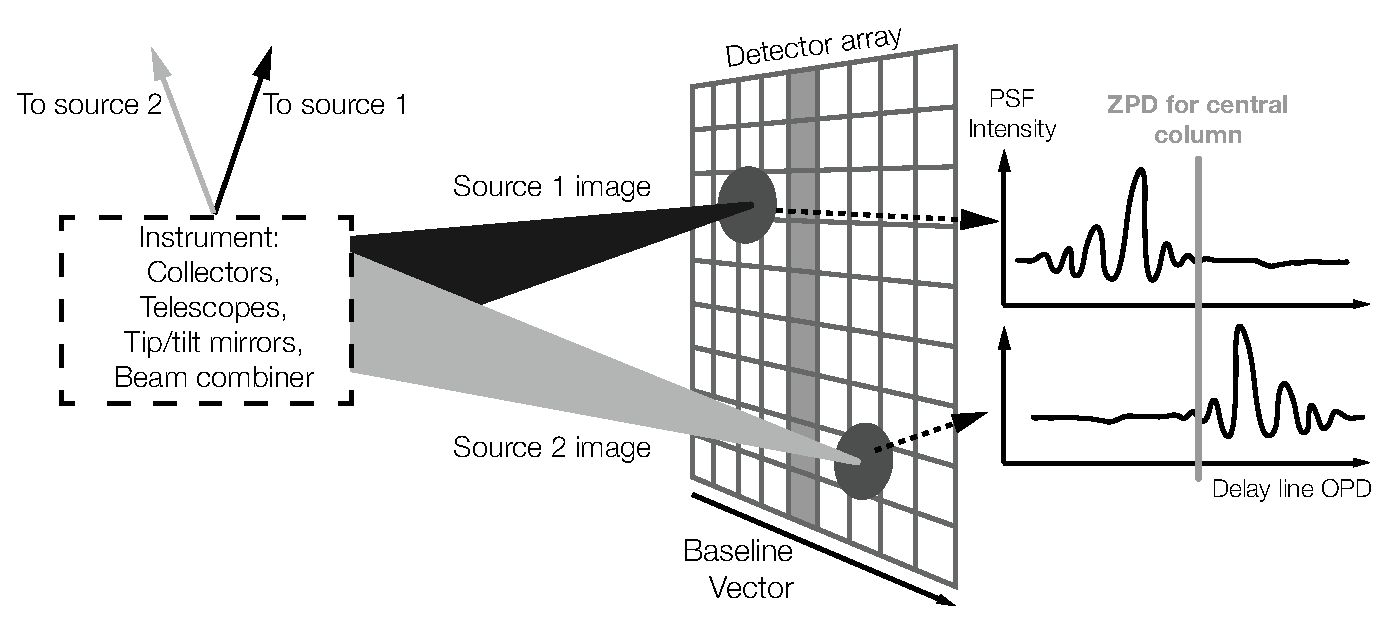
\includegraphics{Figures/f1.eps}
\caption[WideField]{Concept of wide-field double-Fourier interferometry. Light from the instrument is focused after combination to an image of the sky on the detector array (represented as the grid). Each column of the detector has a distinct ZPD so the interferometric responses (right side) of two sources on different columns are centered around different delay positions. The gray stripe represents the central column on the detector array and its corresponding ZPD on the interferograms.}
%The instrument is represented by the double-headed arrow to the left. This encompasses the light collectors, the telescopes, the tip/tilt correction stages, the pupil re-imagers, and the beam combiner. After the beam combiner, the beam is focussed onto the detector array shown in this picture. Changing the OPD modulates the intensity of the Airy disks of each source in the field, and we get interferograms, as shown to the right. In this sketch we suppose that the baseline is aligned with the rows on the detector. Hence, each column of pixels always has the same instrumental OPD. In the general case, pixels along a line perpendicular to the baseline have the same OPD. Further, each source at an angle $\theta$ from the central column has an external OPD equal to $|\baseline |\sin\theta$. When the instrumental OPD approaches the opposite of this value, fringes can be seen for the source.}
\label{fig:widefield}
\end{center}
\end{figure}

\begin{figure}[ht!]
\begin{center}
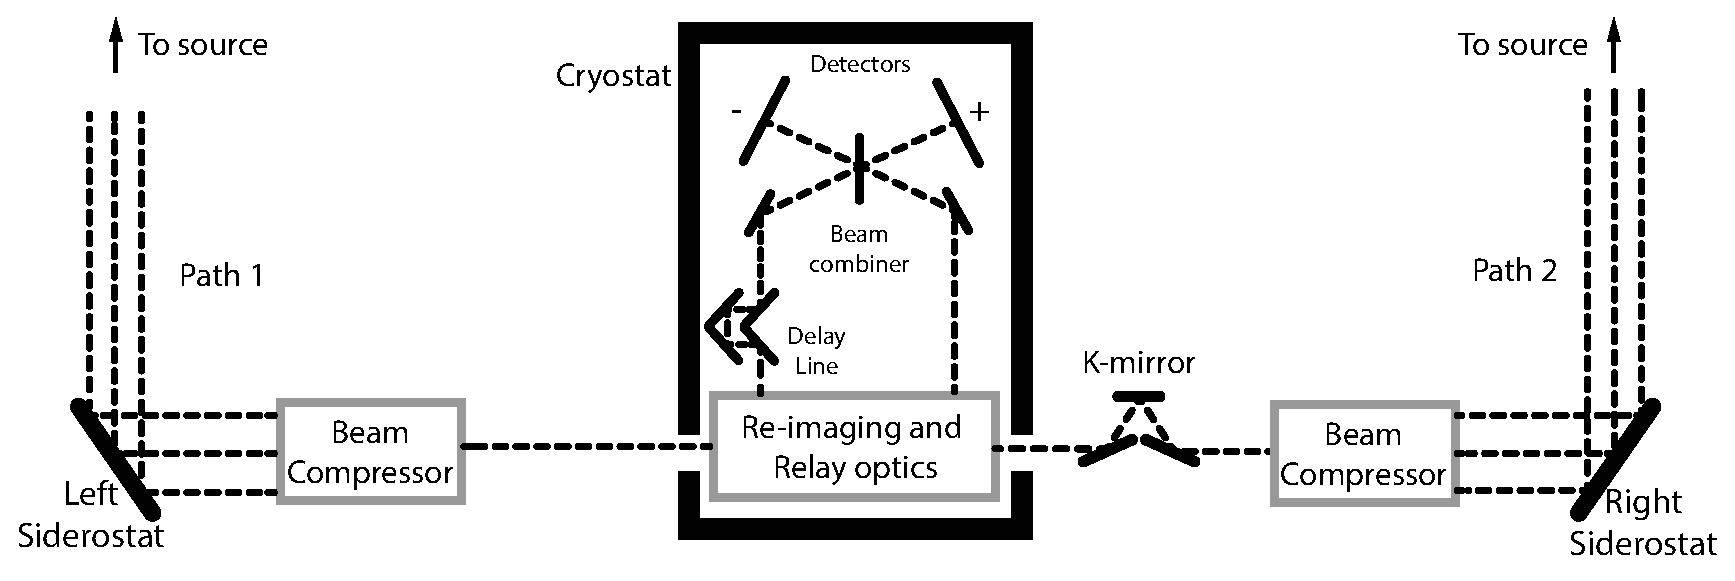
\includegraphics{Figures/f2.eps}
\caption[optics]{Optical train diagram of a typical far-IR, double-Fourier instrument. The K-mirror rotates the beam to align the fields of view of the two sides. Inside the cryostat, a set of optics re-image the pupil, implement a controlled instrumental delay between them with the Cold Delay Line, and relay them towards the central beam combiner. After the combiner, the beams are imaged onto the detectors. To see the BETTII-specific implementation of this design, see \cite{2014PASP..126..660R}.}
\label{fig:optics}
\end{center}
\end{figure}

%\begin{comment}
\begin{figure}[ht!]
\begin{center}
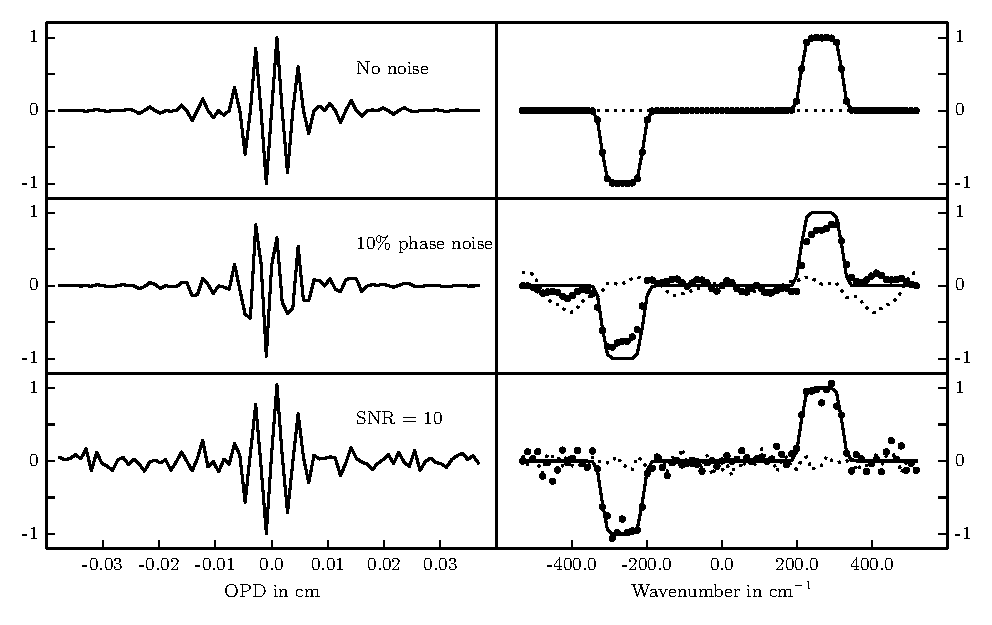
\includegraphics{Figures/f3.eps}
\caption[interfero]{Effects of phase and intensity noise on the recovered spectrum (single realization of the noise). Left column: normalized interferograms, intensity as function of OPD. Right column: normalized DFT of interferograms. Solid: input spectrum multiplied by anti-symmetric transmission function; Solid circles: Imaginary part of DFT from interferogram; Dotted: Real part of DFT. First row: ideal measured signal, no noise; used for normalization of all other plots. Second row: results with a realization of phase noise of 10\% at each point of the interferogram. Third row: results with a realization of intensity noise and $\SNR_\mI=10$.}
\label{fig:interfero}
\end{center}
\end{figure}

%\begin{figure}[ht!]
%\begin{center}
%\plotone{f4.eps}
%\caption[Impact of phase noise]{The phase noise affects the signal more for larger wavenumbers. This shows the simulation for band 1 of BETTII. The amount of phase is quantified by its amount in terms of percentage RMS of the wavelength corresponding to the central wavenumber, about 39 microns (256 cm${-1}$) in our case.}
%\label{fig:PhaseNoiseSim}
%\end{center}
%\end{figure}

%\begin{figure}[ht!]
%\begin{center}
%\plotone{f5.eps}
%\caption[exinter]{Example of simulated recovered spectrum of a 40 Jy source over one 10-minute track with $\R=10$, in the presence of  expected thermal noise levels and phase noise of 10\%. The chosen source spectrum follows a simple power law $\S(\s)\propto\s^2$.}
%\label{fig:exinter}
%\end{center}
%\end{figure}

%\begin{figure}[ht!]
%\begin{center}
%\plotone{f6.eps}
%\caption[Phase Noise]{Residual phase noise profile. The phase noise is expressed in percentage of the central wavelength of the short band (\% of 40~$\um$). }
%\label{fig:SpectralSNR}
%\end{center}
%\end{figure}

%\begin{figure}[ht!]
%\begin{center}
%\plotone{f7.eps}
%\caption[Spectral SNR]{Effects of phase noise and background noise on the spectral $\SNR$. This simulation is computed for BETTII's band 1 parameters and noise estimates, for R=10. We show the results in both the normal science observing mode and the enhanced sensitivity mode. Both simulations are for 200 averaged scans, or 10 minutes on a source. It is important to note that one source can be observed at multiple times during the course of one flight, hence increasing the spectral $\SNR$.}
%\label{fig:SpectralSNR}
%\end{center}
%\end{figure}
%\end{comment}
%\begin{figure}[ht!]
%\begin{center}
%\plotone{f8.eps}
%\caption[Visibility]{Effects of source extension with an 8~m baseline interferometer, for band 1. The visibility at the central wavelength is larger than the integrated visibility over the band, especially given that our band is extremely wide.}
%\label{fig:Visibility}
%\end{center}
%\end{figure}
\begin{figure}[ht!]
\begin{center}
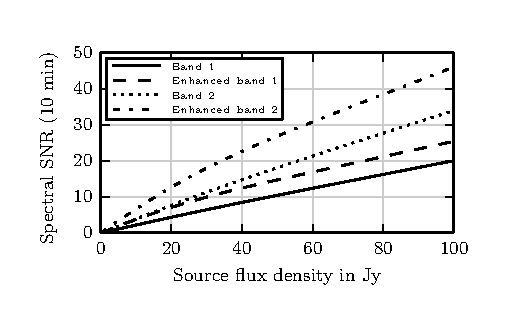
\includegraphics{Figures/f4.eps}
\caption[BETTII Spectral SNR]{%Effects of phase noise and background noise on the spectral $\SNR$. This simulation is computed for BETTII's band 1 parameters and noise estimates, for R=10. We show the results in both the normal science observing mode and the enhanced sensitivity mode. Both simulations are for 200 averaged scans, or 10 minutes on a source. It is important to note that one source can be observed at multiple times during the course of one flight, hence increasing the spectral $\SNR$.
BETTII's spectral sensitivity. Solid: Normal observing mode, band 1; Dashed: Enhanced sensitivity mode, band 1; Dotted: normal observing mode, band 2; Dot-dashed: Enhanced sensitivity mode, band 2. This plot includes the technique of fringe tracking in the science channel for sufficiently bright sources (see Appendix C). As the source flux rises, the effects of the phase noise become larger and the SNR should reach an asymptotical value. However, with fringe tracking, the phase noise itself becomes smaller since one can see fringes in one single or a few consecutive scans, so the co-adding becomes easier. Thanks to the fringe-tracking, there is no regime where the phase noise is expected to be dominant on BETTII, provided that the control system performs according to expectations.}
\label{fig:SpectralSNR}
\end{center}
\end{figure}
 
%% Chapter 3

\chapter[Attitude estimation and control for BETTII]{\setstretch{1}Attitude estimation and control for BETTII} % Main chapter title

\label{chap:controls} % For referencing the chapter elsewhere, use \ref{Chapter1} 

\epigraph{\setstretch{1}\small\itshape Don't bother just to be better than your contemporaries or predecessors. Try to be better than yourself.}{W. Faulkner}



\usetikzlibrary{decorations.markings}





\newcommand{\savedx}{0}
\newcommand{\savedy}{0}
\newcommand{\savedz}{0}
\newcommand{\bettii}[2]%
{   
\pgfmathsetmacro{\boxsize}{#1}
\coordinate (O) at (0,0,0);
\coordinate (Ox) at (#1,0,0);
\coordinate (Oy) at (0,#1,0);
\coordinate (Oz) at (0,0,#1);

\coordinate (a) at (0.5*\boxsize,-4.5*\boxsize,0);
\coordinate (b) at (0.5*\boxsize,4.5*\boxsize,0);
\coordinate (c) at (-0.5*\boxsize,-4.5*\boxsize,0);
\coordinate (d) at (-0.5*\boxsize,4.5*\boxsize,0);
\coordinate (e) at (0.5*\boxsize,-3.5*\boxsize,-\boxsize);
\coordinate (f) at (0.5*\boxsize,3.5*\boxsize,-\boxsize);
\coordinate (g) at (-0.5*\boxsize,-3.5*\boxsize,-\boxsize);
\coordinate (h) at (-0.5*\boxsize,3.5*\boxsize,-\boxsize);
\coordinate (zc1) at (0.5*\boxsize,0.5*\boxsize,\boxsize);
\coordinate (zc2) at (0.5*\boxsize,-0.5*\boxsize,\boxsize);
\coordinate (zc3) at (-0.5*\boxsize,-.5*\boxsize,\boxsize);
\coordinate (zc4) at (-0.5*\boxsize,.5*\boxsize,\boxsize);
\coordinate (Oc1) at (0.5*\boxsize,0.5*\boxsize,0);
\coordinate (Oc2) at (0.5*\boxsize,-0.5*\boxsize,0);
\coordinate (Oc3) at (-0.5*\boxsize,-.5*\boxsize,0);
\coordinate (Oc4) at (-0.5*\boxsize,.5*\boxsize,0);
\coordinate (Bc1) at (0.5*\boxsize,0.5*\boxsize,-\boxsize);
\coordinate (Bc2) at (0.5*\boxsize,-0.5*\boxsize,-\boxsize);
\coordinate (Bc3) at (-0.5*\boxsize,-.5*\boxsize,-\boxsize);
\coordinate (Bc4) at (-0.5*\boxsize,.5*\boxsize,-\boxsize);
\coordinate (Dc1) at (0.5*\boxsize,1.5*\boxsize,0);
\coordinate (Dc2) at (0.5*\boxsize,-1.5*\boxsize,0);
\coordinate (Dc3) at (-0.5*\boxsize,-1.5*\boxsize,0);
\coordinate (Dc4) at (-0.5*\boxsize,1.5*\boxsize,0);




   \draw[thin,#2] (a)--(b) (c)--(d) (a)--(c) (b)--(d) (e)--(f) (g)--(h) (e)--(g) (f)--(h) (a)--(e) (c)--(g) (b)--(f) (d)--(h) (zc1) -- (zc2) (zc2) -- (zc3) (zc3) -- (zc4) (zc4) -- (zc1) (zc1) -- (Dc1) (zc2) -- (Dc2) (zc3) -- (Dc3) (zc4) -- (Dc4) (Dc1) -- (Dc4) (Dc2) -- (Dc3) (zc1) -- (Bc1) (zc2) -- (Bc2) (zc3) -- (Bc3) (zc4) -- (Bc4) (Bc1) -- (Bc4) (Bc2) -- (Bc3) ;
   \draw[thick](zc1) -- (Oc2) (zc4) -- (Oc3) (Oc3) -- (Bc4) (Oc2) -- (Bc1);
%   \draw[->,thick] (O) -- (Ox) node[right] {x};
%   \draw[->,thick] (O) -- (Oy) node[right] {y};
%   \draw[->,thick] (O) -- (Oz) node[right] {z};
%    \fill (a) circle (0.1cm);
%    \fill (d) ++(0.1cm,0.1cm) rectangle ++(-0.2cm,-0.2cm);



}


\tikzset{
%Define standard arrow tip
>=stealth',
%Define style for different line styles
help lines/.style={dashed, thick},
axis/.style={<->},
important line/.style={thick},
connection/.style={thick, dotted},
}

\renewcommand*{\arraystretch}{0.75}
%----------------------------------------------------------------------------------------

%\section{Derivation of requirements from the science}

Chapter~\ref{chap:phasenoisepaper} sets the general background to double-Fourier interferometry when used mostly in spectroscopy mode. It sets the mathematical formalism to estimate the spectral sensitivity, given various sources of gaussian noises. 

In this section, we see more directly how this applies to BETTII, and how the system is designed to satisfy these requirements in order to guarantee good observations.

\subsection{	Relevant timescales (flows well because it is relevant to chapter 2)}
\subsection{	Expected perturbations}
\subsubsection{	High-altitude winds and pendulum motions}
Insert here the picture of the pendulum mode showing the error introduced due to mispointing
\subsubsection{	High-frequency embedded perturbations}
Show here a PSD of the noise spectrum recorded by the gyroscopes, when it is lifted and the wheels are on/off, and when it is on the ground with the wheels on
Need the wheels to be synchronized...
\subsection{	Perturbation rejection requirements }
\subsection{	Required control performance}
\subsection{	Required knowledge performance}


%----------------------------------------------------------------------------------------

\section{Control system architecture}
\label{sec:Chap3-ControlSystemArchitecture}
Chapter~\ref{chap:phasenoisepaper} sets the general background to double-Fourier interferometry when used mostly in spectroscopy mode. It sets the mathematical formalism to estimate the spectral sensitivity, given various sources of gaussian noises. 

In this section, we see more directly how this applies to BETTII, and how the system is designed to satisfy these requirements in order to guarantee good observations.

\subsection{Overall strategy}

\subsubsection{Requirements}
The strategy that we developed aims at satisfying the requirements established in the previous section, under the cost, time and personnel constraints that we were subject to. It fundamentally relies on the fact that \textit{knowledge} is more important than \textit{control}. While several research groups [CITE WASPS] are attempting to provide sub-arcsecond balloon gondola control, we are not going to. This strategy uses the fundamental advantage that the interferometer has over traditional pointed observatories: the decoupling of the phase with the pointing. This feature of interferometers refers to the possibility of obtaining electromagnetic interference even when the telescopes are slightly mispointed from the target. 

There three levels of requirements for our instrument to produce interferograms. First, both arms need to be pointed at the target, so that an image of the target seen through each arm is formed at the detector. For our purpose this will largely be set by the limitation of the field of view of the instrument, which is about 2 arcminutes. When a target is not exactly on-axis with the telescope, it can still fall on the detector if tip/tilt correction happens downstream. The tip/tilt correction will create aberrations, but these are relatively well behaved at our wavelengths. Hence, this requirement can be expressed as an overall pointing requirement of the instrument to some amount that can be corrected in tip/tilt in each individual arms. We set this to $\pm\ang{;;15}$. This also roughly corresponds to one single pixel on the short band detector, and half a primary beam's FWHM.

Once the instrument is pointed to the desired target to within $\pm\ang{;;15}$, there needs to be a fine guiding system in each arm that allows for the remaining correction. This level of control needs to overlap the beams to a small fraction of a pixel to get maximum overlap and minimum visibility losses. We set this requirement to \ang{;;1.5} r.m.s., which corresponds to a tenth of a pixel's size. The fine guidance system needs to operate over a range of at least $\pm\ang{;;15}$ to pick up where the previous level of requirements stops. It also needs to happen with high bandwidth to ensure that only minimum motion is occurring at timescales comparable to a data acquisition timescale. This system is described in section [].

Finally, an angular mispointing of the baseline vector with respect to the target can be might still exist, even if both beams are overlapped properly. This introduces an unwanted optical delay that can push the fringe packets outside our nominal OPD scanning range. Control of this optical delay is critical for interferometry, as it is required to properly reconstruct the OPD axis of the interferograms that are the elementary data blocks of the instrument. This can be achieved using a delay line . This is commonly done for all interferometers on the ground [CITE], and we will implement a device like this on BETTII as well [section]. For this to work, we need to be able to monitor the changes in OPD accurately, which is equivalent, on short timescales, to accurately estimate the attitude of the payload.


%\begin{figure}[!ht]
%	\centering
%	\includestandalone{Figures/InterferometryBaseline}
%	\caption[Relationship between pointing error and OPD]{Relationship between pointing error and OPD}
%	\label{fig:interferometrybaseline}
%    \end{figure}
%

A good estimate of the attitude of our payload can lead to an accurate angular difference between our baseline vector and our target. This angular difference can be converted to an OPD using simple geometric arguments, and can then be fed to the delay line for correction. With an 8~m baseline length, an mispointing of \ang{;;1} along the baseline direction corresponds to an OPD of about \SI{40}{\um}, or one full wavelength of BETTII's short-wavelength band. In order to produce quality interferograms, we will need to know the OPD to a fraction of this [SEE previous section]. 



\subsubsection{Control loop design and operating modes}

The three levels of control that we need are:
\begin{enumerate}
\item Coarse control of the entire gondola to within $\pm~$\ang{;;15} of the target,
\item Fine pointing control of each beam to \ang{;;1.5} r.m.s. at the science detector,
\item Fine knowledge of the inertial attitude to $\approx$~\ang{;;0.15} r.m.s., followed by appropriate OPD control
\end{enumerate}

At its fundamental level, the problem is to implement a system that satisfies these requirements, starting with only the target's location in right ascension (RA) and declination (DEC). Ideally, the system needs to be able to achieve these goals autonomously. All of the operating modes follow from this.

All of the pointing will be done in the reference frame of the gondola, which is tied solidly to the reference frame of the gondola (nominally they are the same) and the star cameras (nominally off by \SI{-45}{\degree} about the $\vectors{y}$~axis. In the following sections, we describe how the inertial attitude of the gondola is determined. Once it is known, a target's RA and DEC can be converted to a desired local azimuth $\Az$ and elevation $\El$ in the spherical coordinates attached to the gondola reference frame (see Fig.~\ref{fig:AzEl}). It is important to note that when we mention "azimuth", we are not referencing to any cardinal directions, as it can be done for other applications. For us, an azimuth is one of the two spherical angles that describe the position of our target in the current gondola reference frame. Note that the elevation angle is defined as being zero in the ($\vectors{x}_\gyro$,$\vectors{y}_\gyro$)-plane.

\begin{figure}[!ht]
	\centering
	\includestandalone{Figures/AzEl}
	\caption[Azimuth and elevation of a target]{}
	\label{fig:AzEl}
    \end{figure}


Once the turbulence from the ascent have died out, the control system determines where the gondola is currently pointing using the star cameras. For the software to process the star camera image, the payload has to be still to avoid blurring of the stars on the CCD. Hence, the first order of business is to slow down the payload's inertial velocity, which is measured by the gyroscopes. This is also called $\BRAKE$ mode.

The first time the system receives a star camera frame and identifies its inertial position, this triggers the estimator algorithm that constantly combines gyroscope and star camera information. From this point on, we have a reasonable estimate of where the gyroscope reference frame is pointed in the inertial frame at all times. 

When a new target in RA and DEC is set by the flight computer, the system will enter the $\SLEW$ mode. This creates a profile of desired azimuth position and velocity as a function of time. The software actuates the reaction wheels to turn the payload about its $\vectors{z}$ axis. At the same time, it commands the rotation stages that control the telescopes' elevation, to go to the desired elevation. The control in elevation and control in azimuth are entirely decoupled.

When we complete the deceleration phase as we get close to our target, we switch to $\TRACK$ mode. This mode is attempting at maintaining control of the telescope within $\pm$~\ang{;;15} of our target.

Finally, for each of the two arms, we need to acquire a guide star onto our guide camera [section]. This requires a fast imaging capability and a fast-steering tip/tilt correction mechanism to freeze the motion of the sky on the guide camera. This is $\ACQUIRE$ mode. Two images of the sky are made on the detector, one from each arm; the guide star is located in each image, and the tip/tilt mechanisms are actuated to center this star onto a location of the detector that corresponds to maximum overlap at the science detectors. One the star is centered onto that location, the window size of the camera decreases, and the acquisition speed increases. Ultimately, we will get two patches of 35$\times$35 pixels at $\approx$~\SI{50}{\hertz}. When this acquisition speed is reached we consider ourselves in $\LOCKED$ mode.

In both $\ACQUIRE$ and $\LOCKED$ mode, the position of the two tip/tilt platforms contains information on the overall mispointing of the optical train: when the actuators are both off in the same direction with respect to their nominal position, it means that the entire truss is off the guide star by this amount. When available, this information is used by the estimator along with the gyroscope and star camera information to compute the best possible attitude estimate. Since the tip/tilt is tied to the actual optics train, its information is heavily weighted compared to the other sensors. 

When the two guide star images are centered, this means proper overlap of the far-infrared beams at the science detectors. Hence, we are in a position to spot interferometric signal, which will translate to a modulation of the intensity of the coherently combined image as a function of OPD. The OPD is constantly modulated with the Cold Delay Line [section], independently of the mode in which we are. However, residual mispointings can create large unwanted OPD perturbations. Hence, during $\TRACK$ and $\ACQUIRE$ mode, the Warm Delay Line mechanism is activated. Its goal is to use the estimated change in baseline position to predict the resulting OPD variations - and correct them directly in OPD space. 

During the $\LOCKED$ mode, we need to consider what happens if we lose the guide star. Since the field of view is relatively small compared to the expected motions of the gondola, the guide star could technically walk outside the range of the guide camera - at which point the attitude estimation relies temporarily on the gyroscopes as we switch back to $\ACQUIRE$ mode and the guide camera increases its field of view (and decreases its speed) until it finds the guide star.

\renewcommand{\arraystretch}{1.5}
\newlength\mylen
\settowidth\mylen{\textbullet}
\addtolength\mylen{-3mm}
\setlist[itemize,1]{nolistsep,leftmargin=*,labelsep=-\mylen}
\def\labelitemi{--}
\begin{table}[htbp]
\small
\begin{longtable}{cp{5cm}p{2.5cm}p{3.5cm}}
\toprule
Mode  & Description &  Actuators & Sensors \\
\midrule
$\SAFE$ & All PID gains set to 0; siderostats point towards zenith; azimuth is not commanded;  used during ascent, emergencies &
\begin{minipage}[t]{\linewidth}%
\begin{itemize}[align=parleft]
\item CDL
\end{itemize}
\end{minipage} &
\begin{minipage}[t]{\linewidth}%
\begin{itemize}[align=parleft]
\item Gyros
\item Star cameras
\end{itemize}
\end{minipage} \\
\hline
$\BRAKE$ & Used to slow down the payload after undesired motion; derivative gains only, no position loop & 
\begin{minipage}[t]{\linewidth}%
\begin{itemize}[align=parleft]
\item CCMG 
\item Rotators
\item  CDL
\item  Mom. Dump
\end{itemize}
\end{minipage} &
\begin{minipage}[t]{\linewidth}%
\begin{itemize}[align=parleft]
\item Gyros
\item Star cameras 
\item Elevation encoder 
\item Gimbal encoder
\end{itemize}
\end{minipage} \\
\hline
$\SLEW$ &Used to move to target with a set velocity profile &
\begin{minipage}[t]{\linewidth}%
\begin{itemize}[align=parleft]
\item CCMG 
\item  Rotators
\item  CDL
\item  Mom. Dump
\end{itemize}
\end{minipage} &
\begin{minipage}[t]{\linewidth}%
\begin{itemize}[align=parleft]
\item Gyros 
\item Star cameras  
\item Elevation encoder  
\item Gimbal encoder
\end{itemize}
\end{minipage}\\
\hline
$\TRACK$ & Used to stabilize payload after slew, track target coarsely &
\begin{minipage}[t]{\linewidth}%
\begin{itemize}[align=parleft]
\item CCMG 
\item  Rotators
\item  CDL
\item  Mom. Dump
\item  WDL
\end{itemize}
\end{minipage} &
\begin{minipage}[t]{\linewidth}%
\begin{itemize}[align=parleft]
\item Gyros
\item  Star cameras 
\item  Elevation encoder 
\item  Gimbal encoder
\end{itemize}
\end{minipage}\\
\hline
$\ACQUIRE$ & The guide camera grabs images for each arm and identifies the location of a guide star in increasingly smaller quadrant sizes &
\begin{minipage}[t]{\linewidth}%
\begin{itemize}[align=parleft]
\item CCMG 
\item  Rotators
\item  CDL
\item  Mom. Dump
\item  WDL 
\item Tip/Tilts
\end{itemize}
\end{minipage}&
\begin{minipage}[t]{\linewidth}%
\begin{itemize}[align=parleft]
\item Gyros
\item  Star cameras 
\item  Elevation encoder 
\item  Gimbal encoder 
\item  Tip/Tilt encoders
\item  Guide camera
\end{itemize}
\end{minipage} \\
\hline
$\LOCKED$ & The intensity of the target in the science detector is measured, and the central phase is estimated &
\begin{minipage}[t]{\linewidth}%
\begin{itemize}[align=parleft]
\item CCMG 
\item  Rotators
\item  CDL
\item  Mom. Dump
\item  WDL 
\item  Tip/Tilts
\end{itemize}
\end{minipage}&
\begin{minipage}[t]{\linewidth}%
\begin{itemize}[align=parleft]
\item Gyros
\item  Star cameras 
\item  Elevation encoder 
\item  Gimbal encoder
\item  Tip/Tilt encoders
\item  Guide camera 
\item  Science detector
\end{itemize}
\end{minipage} \\
\bottomrule
\end{longtable}
\caption[Operating modes]{BETTII operating modes. Each operating mode has a set of PID gains for each individual loop.}
\label{tab:modes}
\end{table}

Note that the Cold Delay Line (CDL) is running in closed loop during all the modes. Since the environment inside the cryostat is not changing from test to flight, there is no reason to ever turn the loop off or keep different sets of gains for different operating modes. The CDL is its own closed system.



\subsubsection{BETTII Coordinate systems}


\begin{figure}[!ht]
	\centering
	\includestandalone{Figures/BETTII_coordinate_system}
	\caption[BETTII coordinate systems]{}
	\label{fig:CoordinateSystem}
    \end{figure}

    
%     \begin{figure}[!ht]
% 	\centering
% 	\includestandalone{Figures/starCameraRefFrame}
% 	\caption{Star camera angles. The star camera reference frame as well as the telescope reference frame are represented here with the celestial sphere local RA and DEC axes in the background. There is a known matrix that transforms the star camera reference frame, where inertial attitude is measured, to the telescope reference frame, where error vectors are computed. The error vector is determined on the plane of the sky and has two projections on the telescope reference frame. The $\Delta\El=\Delta$El component corresponds to the elevation error and is corrected by the siderostat angle. The $\Delta\xEl=\Delta$xEl component corresponds to the cross-elevation error, and is corrected by the CCMG gimbal angle. Note that as the siderostat elevation is adjusted to reduce the elevation error, the transformation matrix between the star camera and telescope reference frames is adjusted as well.}
% 	\label{fig:starcamRefFrame}
%     \end{figure}


\begin{figure}[!ht]
	\centering
	\includestandalone{Figures/CelestialSphereRAandDEC2}
	\caption[The celestial sphere]{}
	\label{fig:celestialSphere}
    \end{figure}

\begin{figure}[!ht]
	\centering
	\includestandalone{Figures/starCameraRefFrame}
	\caption[The star camera reference frame]{}
	\label{fig:starcamRefFrame}
    \end{figure}


\subsection{Subsystems}



\subsubsection{Gyroscopes}

\paragraph{Sensitivity tests}
We purchased three SRS-2000 fiber-optic gyroscopes from Optolink. This gyroscope technology uses the Sagnac effect and is the cutting edge in inertial rotational velocity measurements \citep[for a review of the state-of-the-art see, \textit{e.g.}][]{ElBadaoui:2014fr}. We chose these devices for their incredibly low angular random walk, which is a measure of their inherent noise. If we were to trust the gyroscope measurement and integrate its velocity to obtain a position estimate, the estimation error we would make after 1 hour of integration has a standard deviation of about 2 arcseconds.

The devices have a bandwidth of \SI{50}{\hertz}, but can be triggered at up to \SI{2000}{\hertz}. Their extreme stability is contingent upon proper temperature stabilization, which is done with a closed-loop set at their calibration temperature of $\SI{23.5}{\celsius}\pm\SI{0.5}{\celsius}$ using an active built-in Peltier element. This Peltier element transforms electric power into either heating or cooling \citep{Peltier:1834vu}.

However, their sensitivity has complicated some of their testing. As soon as we attach a gyroscope to any structure, it measures its vibrational modes, which makes it hard to make a stable measurement of the gyroscope's drift stability. This includes the vibrations that are inherent to the building in which they are placed.

We were successful at measuring the gyroscope properties over long periods of time by attaching them flush to a heavy slab of metal, and putting the slab of metal flush on the vibration-isolating floor of one of NASA Goddard's optics labs in building 34.

We proceeded to an identical series of tests for each gyroscope:
\begin{enumerate}
\item We acquired data at \SI{2000}{\hertz} for \SI{10}{\minute} to measure a proper power spectral density and characterize the noise;
\item We acquired data at \SI{100}{\hertz} for $\sim$ \SI{8}{\hour} to study the drift properties.
\end{enumerate}

The properties that we are looking for are typical instantaneous angular random walk, and the overall drift instability of the gyroscope's mean. When the gyroscopes are set on the floor, they measure a component of the Earth's rotation vector in inertial space. The mean of the measurement depends on the exact angle at which the device is placed with respect to the zenith vector, and is of no importance for this noise study. We seek to understand how much the mean varies over long periods of time. To avoid disturbances from the building vibrations (opening/closing of doors, etc), we operated entirely after regular working hours.

\begin{figure}[!ht]
		\centering
		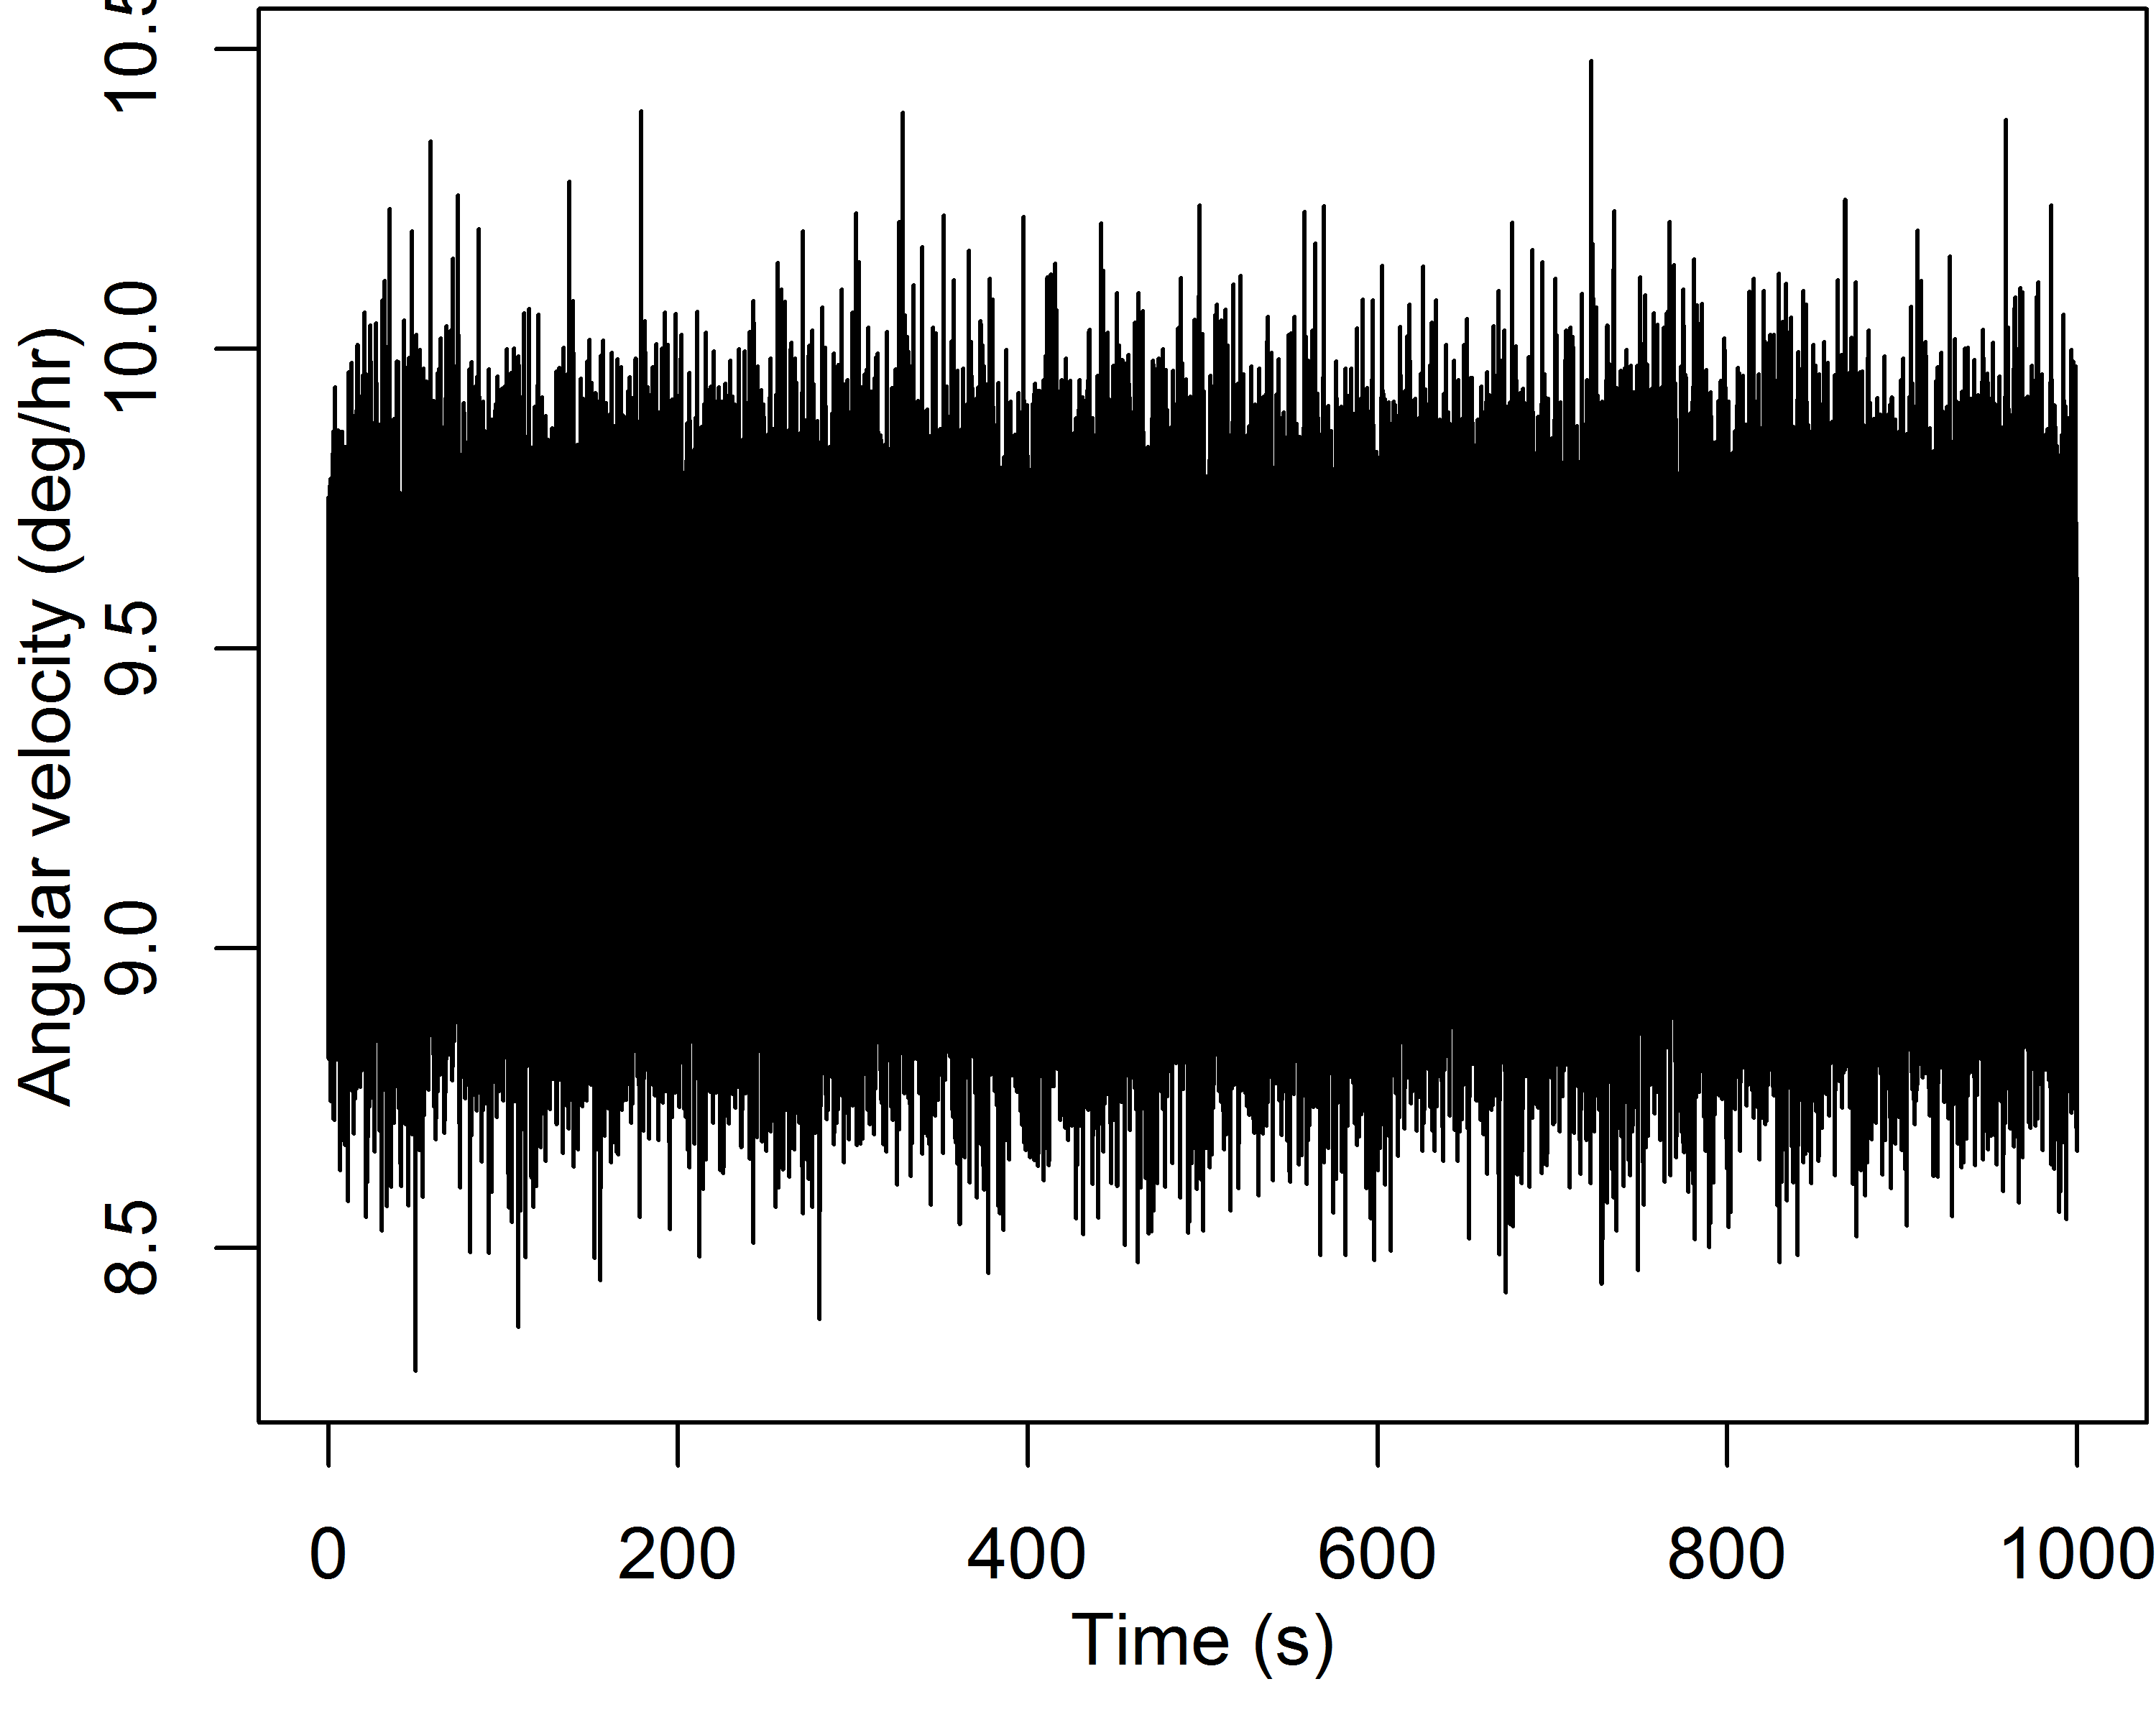
\includegraphics[width=0.98\textwidth]{Figures/snapshot_11005.png} 
		\caption[\SI{1000}{\second} of gyroscope data]{Snapshot of \SI{1000}{\second} of gyroscope data, taken from our \SI{8}{\hour} data sample.}
		\label{fig:snapshot11005}
\end{figure}


The angular random walk (ARW) is a measure of the effects of integrating a noisy velocity measurement. The specification from the manufacturer is ARW = \SI{5e-4}{\deg\raiseto{-0.5}\hour}. This means that if we integrate the gyroscope's rate for 1~hour, the $1-\sigma$ uncertainty on our position would be 
$\SI{5e-4}{\deg}\sim\ang{;;1.8}$. For an integration time of 1 second, it would be \ang{;;0.03}. For a single integration time step $\Deltat = \SI{10}{\milli\second}$, it would be \ang{;;0.003}. 

The manufacturer specification gives a maximum bias instability over a wide range of temperatures less than \SI{0.005}{\deg\per\hour}. This represents how much the mean angular velocity is expected to vary. These tests are an attempt to verify these numbers.


\paragraph{Power spectral density}

The usual frequency-domain analysis tool is the power spectral density (PSD). This allows us to spot any frequency peaks in the data, and let us look at the $1/f$ noise behavior, which is the typical low-frequency behavior that indicates drifts in the signal. The \SI{100}{\hertz} data is all we need, as the gyroscope's bandwidth is \SI{50}{\hertz}. Hence, the \SI{2000}{\hertz} data does not contain any more information than the \SI{100}{\hertz}. In fact, while plotting the PSD of the \SI{2000}{\hertz} data, we can see clearly the break at \SI{50}{\hertz} characteristic of a \SI{50}{\hertz} low-pass filter.

\begin{figure}[!ht]
\begin{subfigure}[b]{0.5\textwidth}

		\centering
		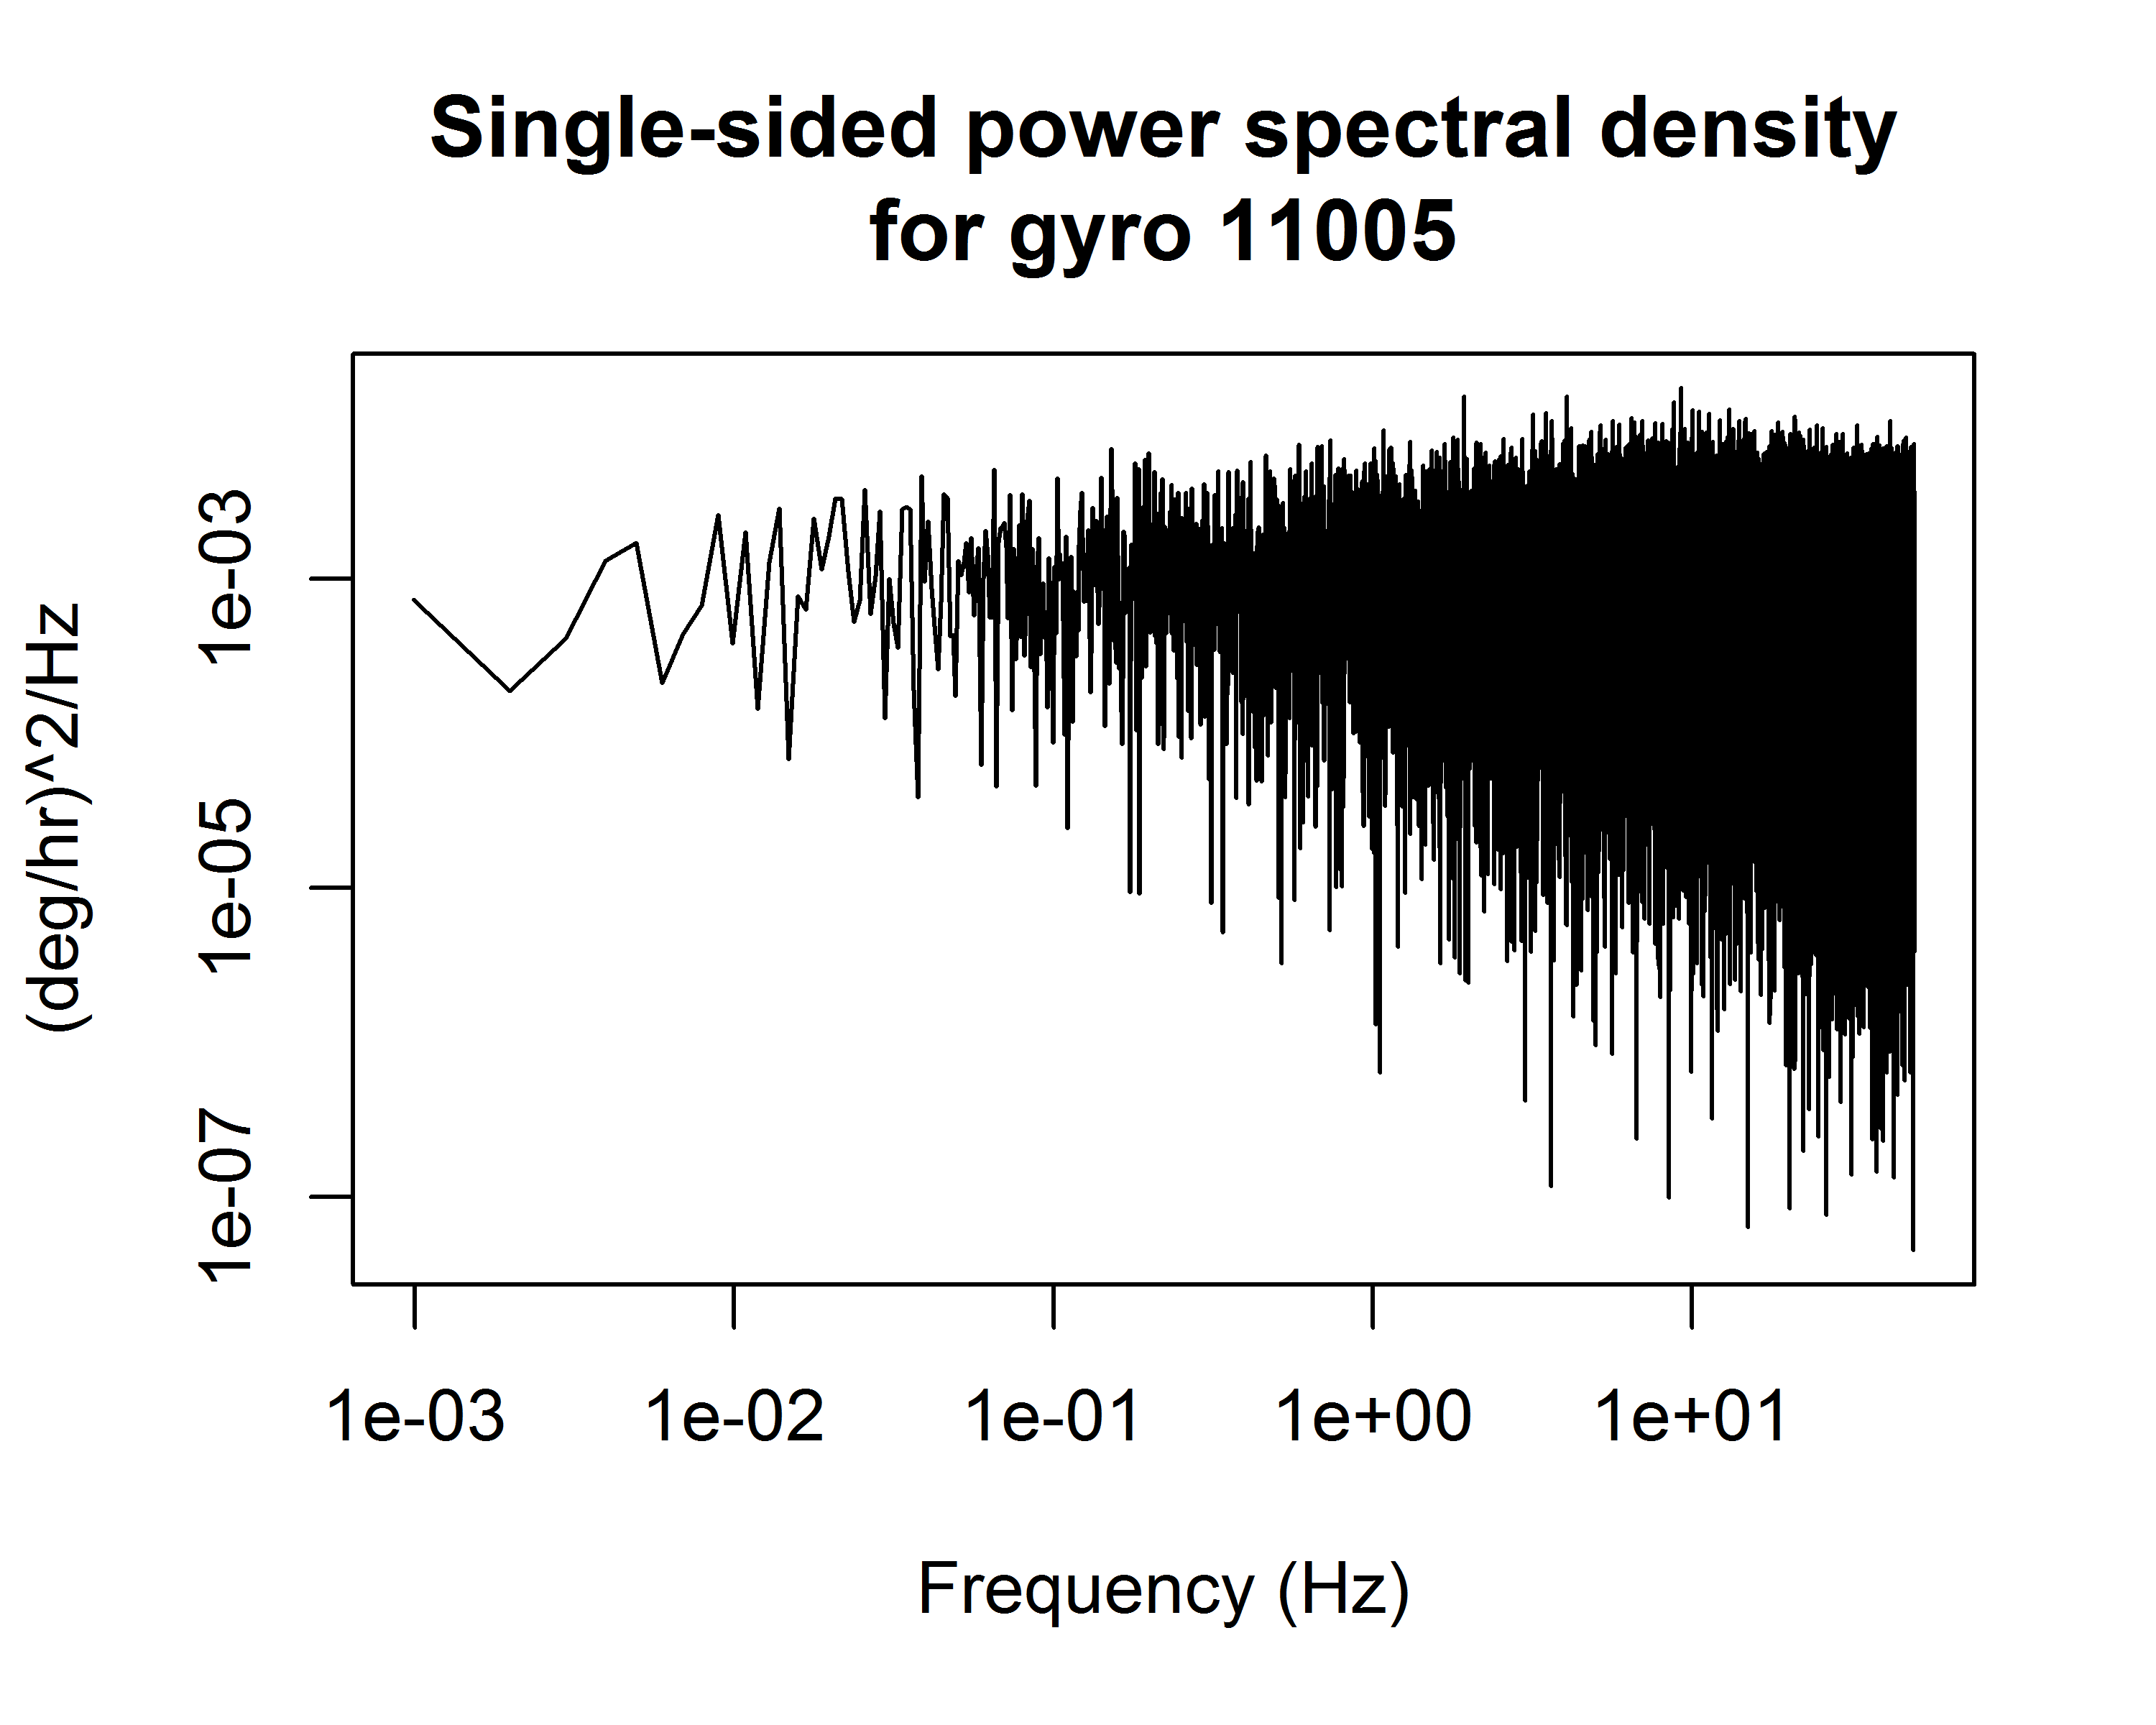
\includegraphics[width=0.98\textwidth]{Figures/sspwsd_11005.png} 
		\caption{}
		\label{subfig:sspsd11005}
\end{subfigure}
\begin{subfigure}[b]{0.5\textwidth}
		\centering
		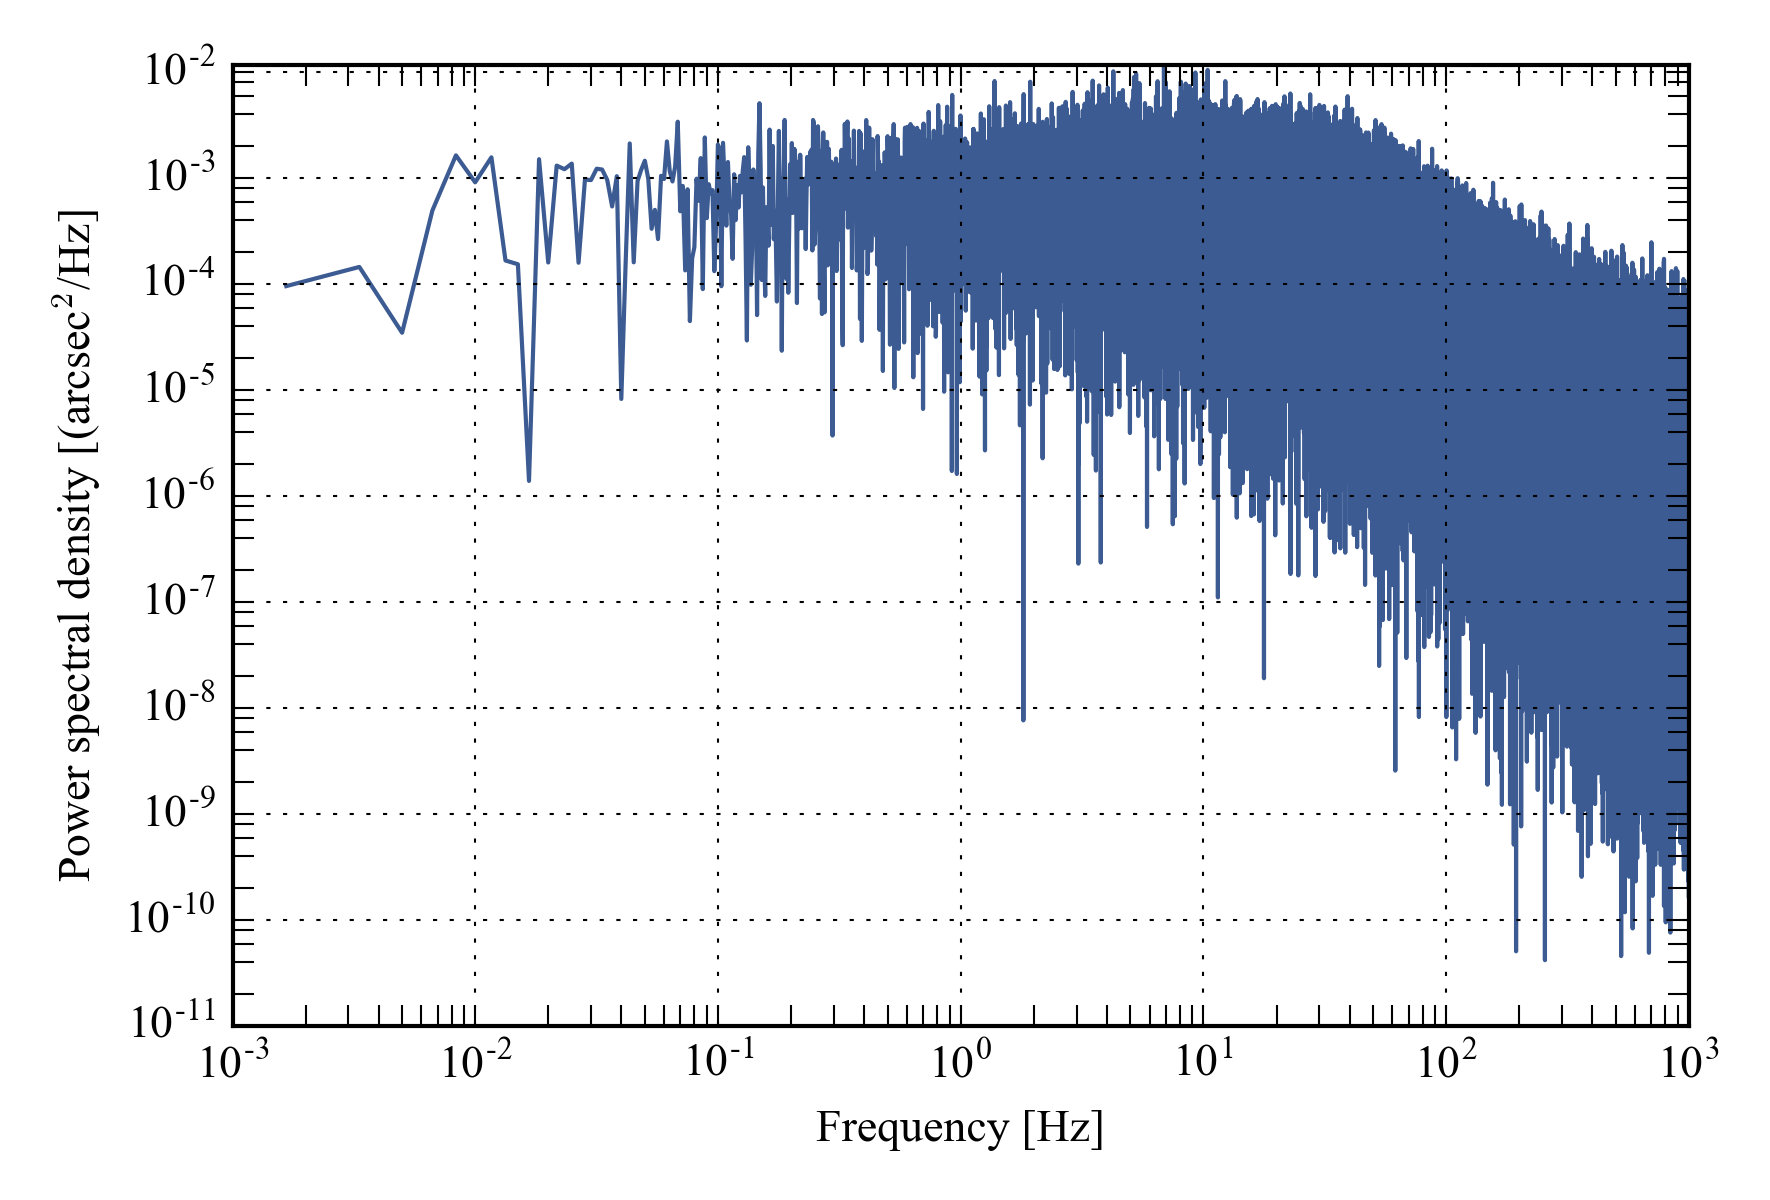
\includegraphics[width=0.98\textwidth]{Figures/sspwsd2000_11005.png} 
		\caption{}
		\label{subfig:sspsd2000-11005}
\end{subfigure}
\label{fig:gyrospectra}
\caption[Power spectral density]{(\subref{subfig:sspsd11005}): Single-sided power spectral density for gyro 11005, an \SI{8}{\hour} sample with a sampling rate of \SI{100}{\hertz}, showing no particular feature (large peaks or resonances). (\subref{subfig:sspsd2000-11005}): Single-sided power spectral density for gyro 11005, a \SI{10}{\minute} sample with a sampling rate of \SI{2000}{\hertz}, showing no electronic resonance peak or other feature. We can notice the \SI{-3}{\decibel} break at around \SI{50}{\hertz}.}
\end{figure}

It is important to note that in their factory settings, the gyroscopes' noise distribution was not normal at all. It exhibited electronic peaks with many harmonics, at frequencies that were varying as a function of the gyroscope inclination (as it was measuring different components of the Earth's rotation). After talking to the manufacturer, we determined that it was caused by the closed-loop algorithms inside the gyroscope electronics. The problem was known by them, and the remedy was to inject a random phase perturbation in the closed loop. This had the effects to get rid of those frequency peaks, at the cost of increasing the overall noise variance by a factor of 4. The noise levels that are specified by the company are very close to the noise seen when using that random phase modulation. Hence, if one does not care as much at the frequency content of the gyroscope, it is possible that this device could work even much better than it does for us.


\begin{figure}[!ht]

\begin{subfigure}[b]{0.5\textwidth}
		\centering
		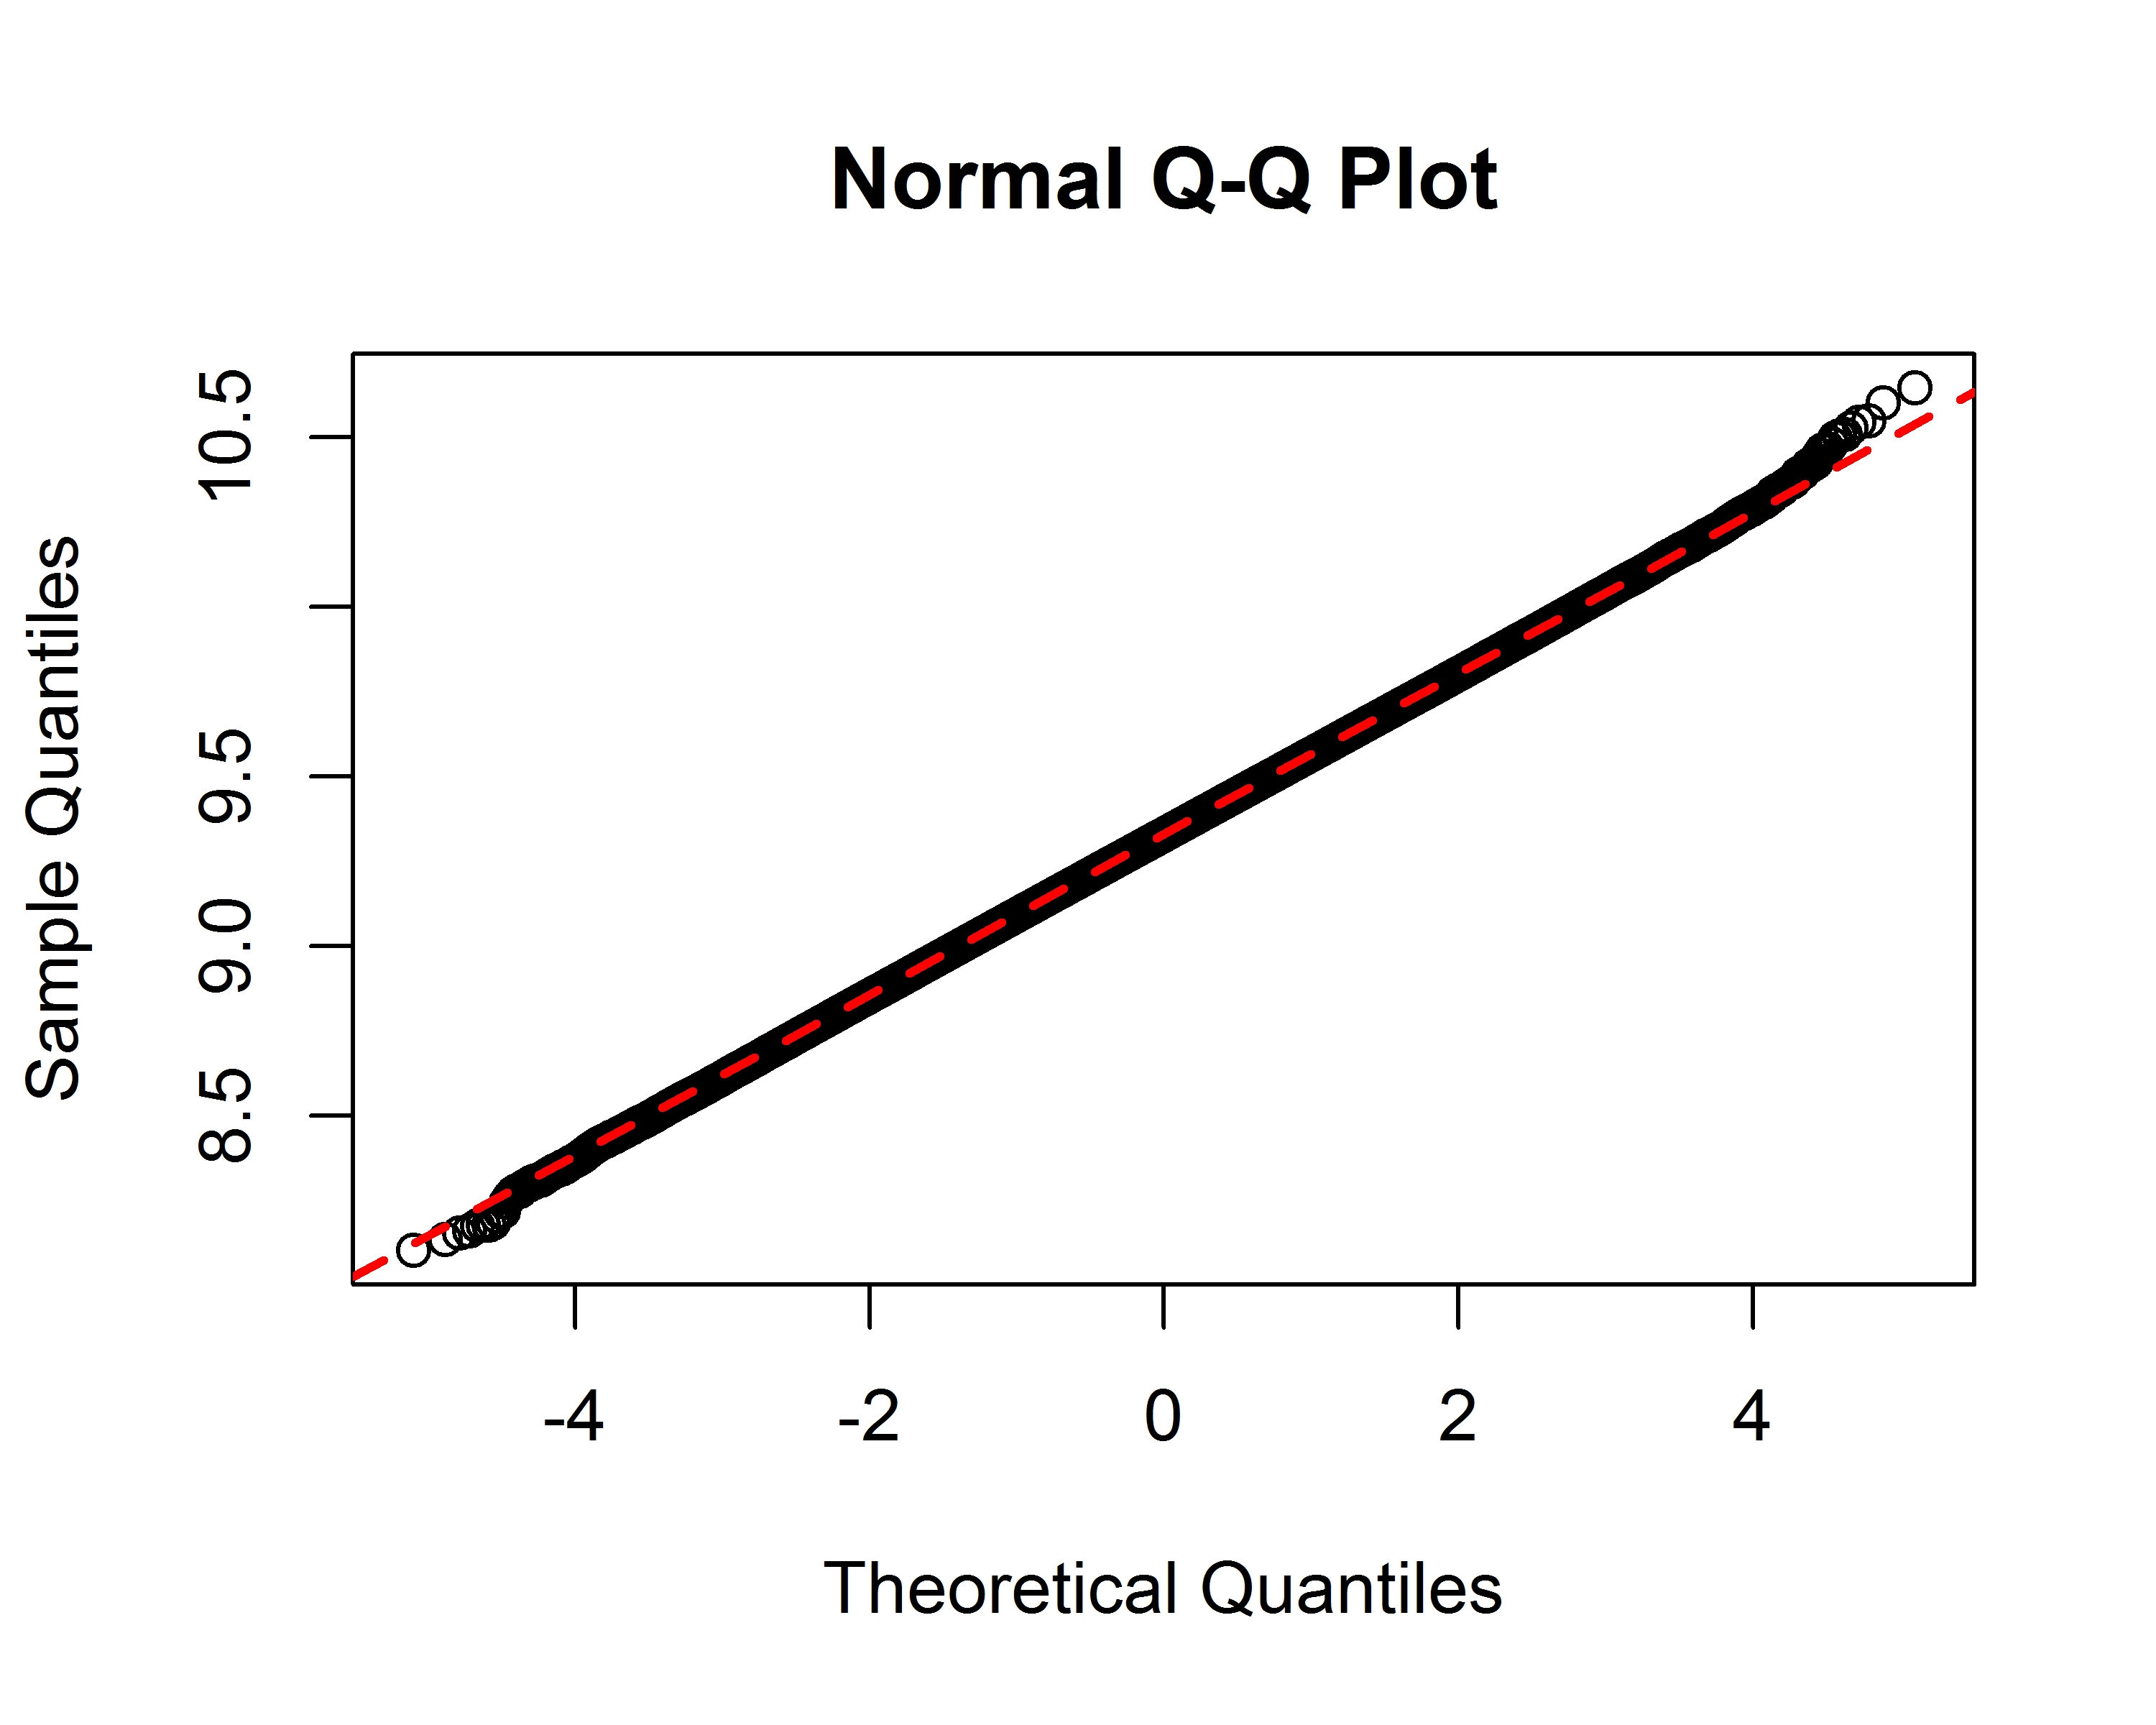
\includegraphics[width=0.98\textwidth]{Figures/qqplot_11005.png} 
		\caption{}
		\label{subfig:probplot11005}
\end{subfigure}
\begin{subfigure}[b]{0.5\textwidth}
		\centering
		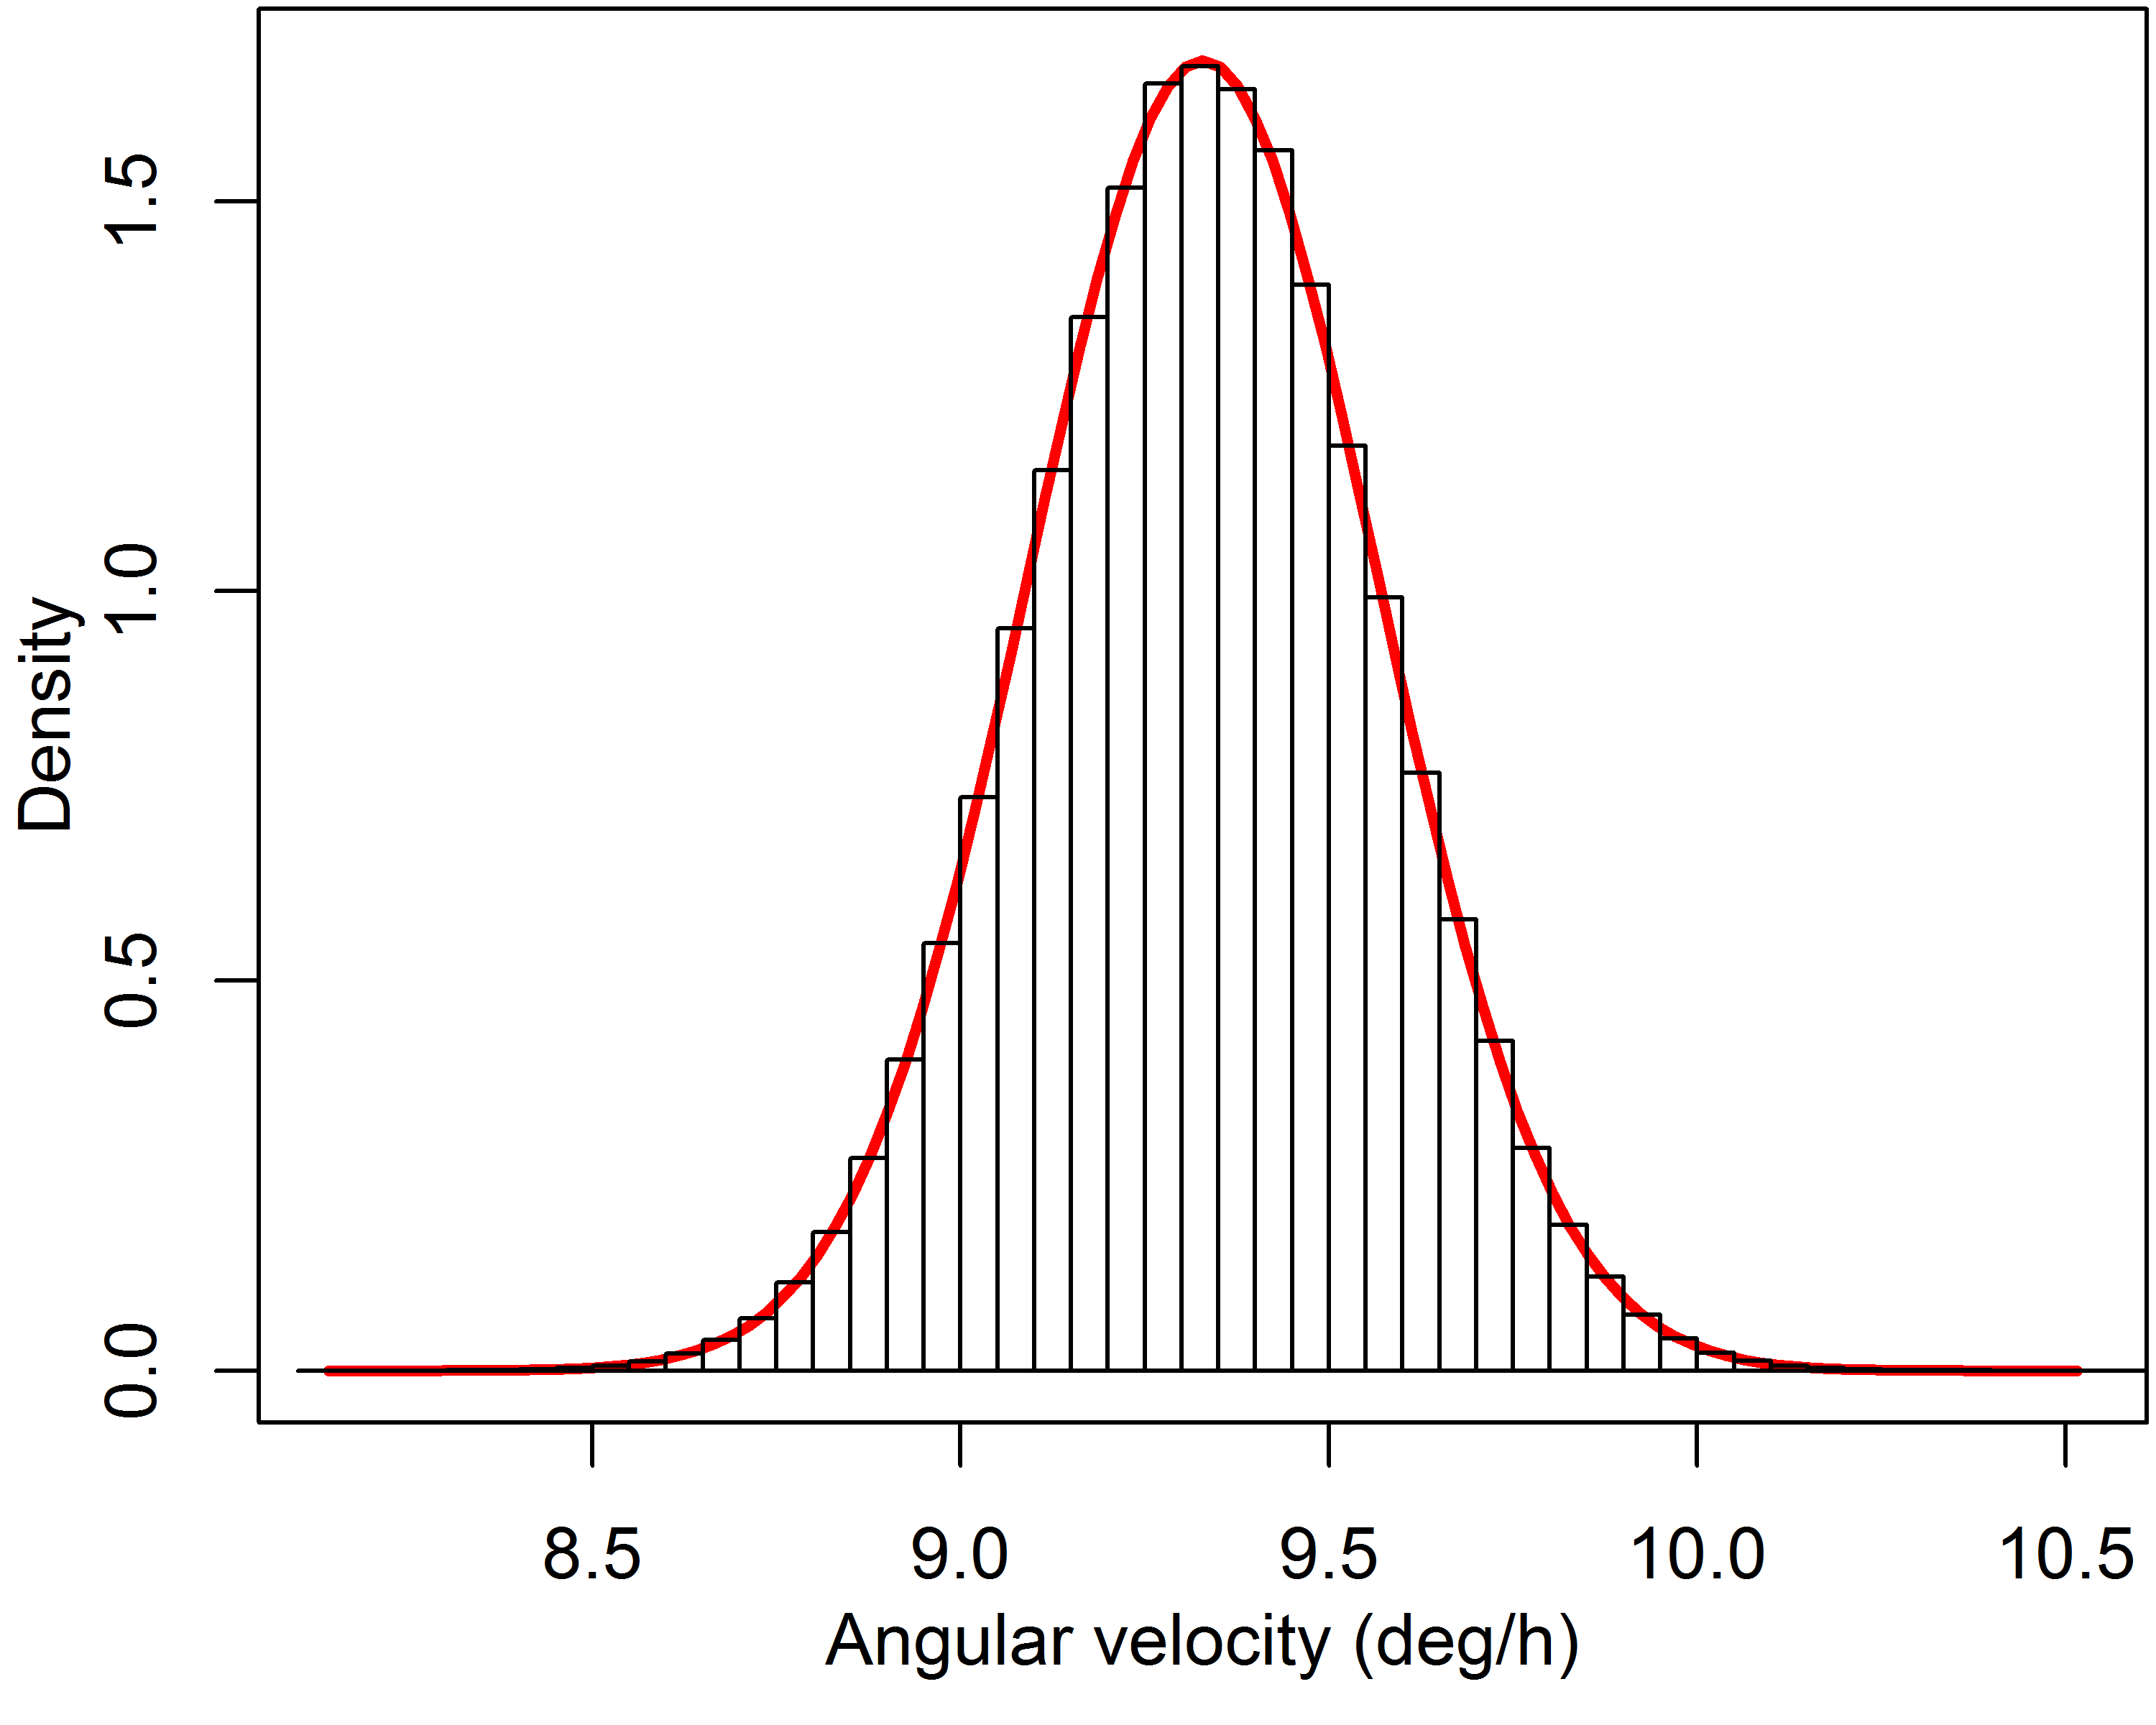
\includegraphics[width=0.98\textwidth]{Figures/distrib_11005.png} 
		\caption{}
		\label{subfig:density11005}
\end{subfigure}
\caption[Normality analysis]{Normality analysis of the gyroscope signal over \SI{8}{\hour} of data taken at \SI{100}{\hertz}. (\subref{subfig:probplot11005}): Normal quantile-quantile plot for an \SI{8}{\hour} sample with a sampling rate at \SI{100}{\hertz}. Here the measured quantiles (fraction of the measured values under a certain value) are plotted against the theoretical quantiles from a normal distribution. The red line is the theoretical distribution if the data were taken from a normal distribution. (\subref{subfig:density11005}): Probability density distribution for an \SI{8}{\hour} sample with a sampling rate at \SI{100}{\hertz}. In red, the theoretical normal distribution we obtain with the measured mean and standard deviation from the sample. While the data is not strictly normally distributed, we consider that it is sufficiently close to a gaussian distribution.}
\label{fig:gyroprobdensity}
\end{figure}

\paragraph{Normality tests}

We ran a few standard normality tests on chunks of the 8-hour data for each gyroscope. While the tests on individual small chunks of data never reject the null hypothesis (that the distribution is normal), the distribution of the total 8 hours does with a very high probability, using both the Anderson-Darling and the Kolmogorov-Smirnov test. It means that it is extremely unlikely that the measured noise over \SI{8}{\hour} is coming from a normal distribution.

Since the data is always consistent with being normally distributed over timescales of tens of minutes, after close inspection of the long-term quartile plots and histograms, we determined that it would be safe to consider the distribution as normal for the purpose of our attitude estimator (see Fig.~\ref{fig:gyroprobdensity}). 




\paragraph{Allan variance}


Another common tool to study of the gyroscope's performance is to plot the Allan variance. The Allan variance gives a time-domain analysis of the gyroscope's noise that is complementary to the power spectral density.

The gyroscopes were successfully tested in the environmental chamber, with no noticeable change in performance except a much larger power draw, due to the Peltier element maintaining the fiber temperature.


\renewcommand{\arraystretch}{1.5}
\begin{table}[htbp]
\small
\begin{tabular}{p{5.5cm}p{2.5cm}p{2.5cm}p{2.5cm}}
\toprule
Measured property & Gyro \#11005 & Gyro \#12003 & Gyro \#12004\\
\midrule
Standard deviation (\si{\deg\per\hour}) & 0.237 & 0.199 & 0.217\\

Angular random walk (\si{\deg\raiseto{-0.5}\hour}) & \num{4.31e-4} & \num{3.79e-4} & \num{4.02e-4}\\

Bias instability (\si{\deg\per\hour}) & \num{3.11e-4} & \num{1.8e-3} & \num{3.05e-4} \\
\bottomrule
\end{tabular}
\label{tab:gyroproperties}
\caption[Gyroscope properties]{Properties of the gyroscopes determined from the Allan variance analysis on an \SI{8}{\hour} sample with a sampling rate at \SI{100}{\hertz}. Note that \SI{1}{\deg\per\hour} =  \SI{1}{\arcsec\per\second}, and the Earth rotates at about \SI{15}{\arcsec\per\second} about the line joining the two poles.}
\end{table}



\begin{figure}[!ht]

	\begin{subfigure}[b]{\textwidth}
		\centering
		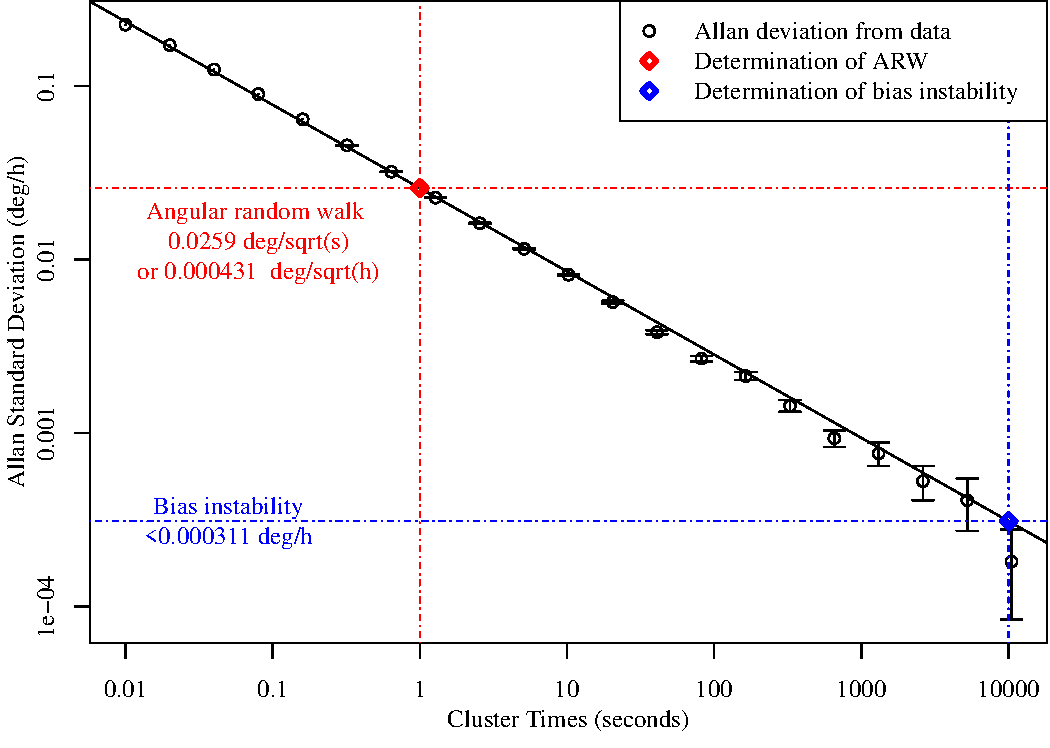
\includegraphics[width=0.98\textwidth]{Figures/allandev_11005.pdf} 
		\caption{Allan deviation of gyro 11005}
		\label{subfig:allan11005}
	\end{subfigure}
	
	\begin{subfigure}[b]{0.5\textwidth}
		\centering
		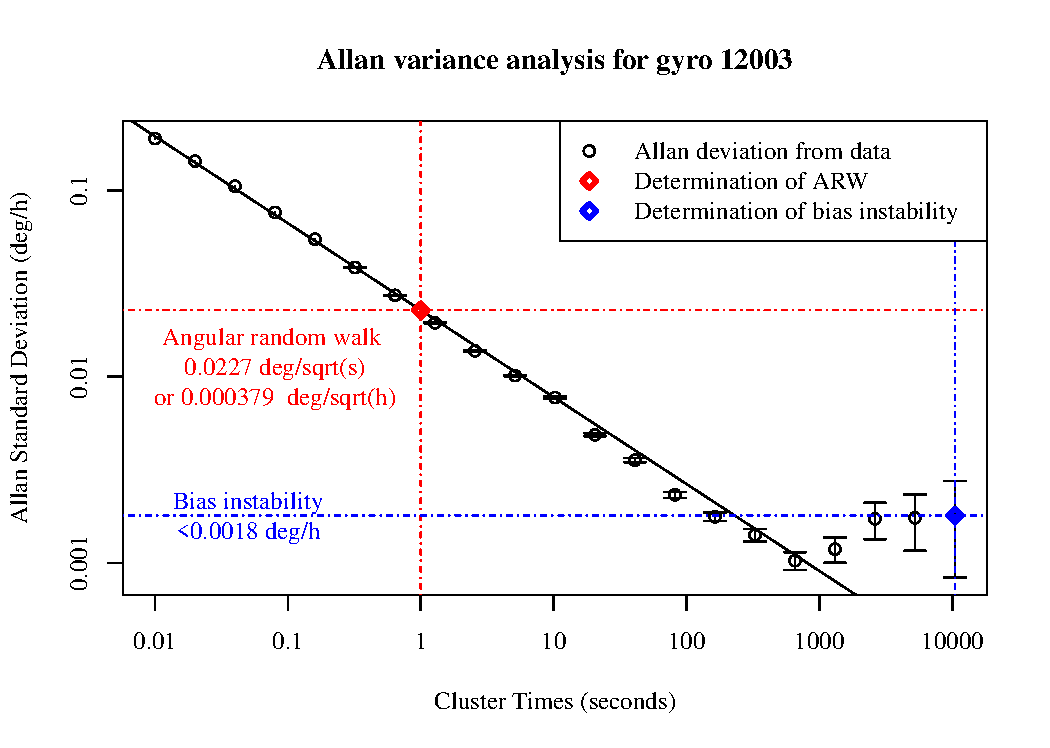
\includegraphics[width=0.98\textwidth]{Figures/allandev_12003.pdf} 
		\caption{Allan deviation of gyro 12003}
		\label{subfig:allan12003}
	\end{subfigure}
	\begin{subfigure}[b]{0.5\textwidth}
		\centering
		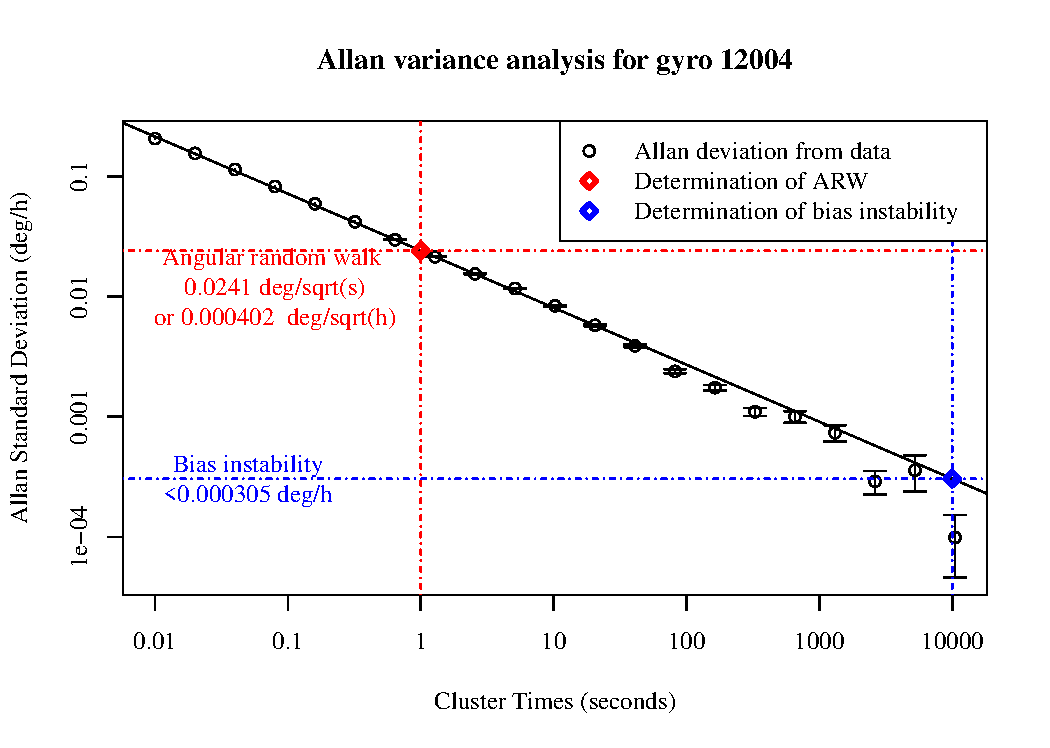
\includegraphics[width=0.98\textwidth]{Figures/allandev_12004.pdf} 
		\caption{Allan deviation of gyro 12004}
		\label{subfig:allan12004}
	\end{subfigure}

\end{figure}

\paragraph{Gyro unit alignment}



\subsubsection{Star cameras}

We have designed, built and tested a custom star camera setup that provides higher accuracy measurements than commercially available devices. Our collaborators from Cardiff University provided the star camera software, which solves for the inertial orientation from a given picture. This software is a C++ set of routines that was originally developed for the EBEX balloon experiment \citep{Oxley:2004hl}. 

Our star camera design features an old-generation Nikon Nikkor \SI{300}{\mm} f/2.8 telefocal lens with manual focus and extended hood. These lenses were manufactured between 1977 and 1982 and can be found today online through websites like e-Bay. The lens provides low chromatic aberration, a magnification of \SI{688}{\arcsecond\per\mm}, a wide field of view ($\approx$~\SI{10}{\degree}) and a collecting area of \SI{90}{\mm\squared} which is is larger than most star tracking assemblies. This old lens does not feature a built-in autofocus or any of the image stabilization actuators commonly found in modern lens assemblies: these could have become a liability in the severe balloon environment. 

Our camera is a USB3.0 Point Grey Grasshopper3. The CCD is a Sony Pregius IMX174 CMOS sensor with 1920$\times$1200 pixels at \SI{5.86}{\um} pitch. This provides a field of view of \SI{2.14}{\degree}$\times$\SI{1.34}{\degree} and a pixel scale of \ang{;;4.02}/pixel. It features a very convenient software suite which works with all the Point Grey camera products, and leaves room for future potential upgrades of the camera. The detector characteristics are summarized in Table~\ref{tab:starcamproperties}.

\renewcommand{\arraystretch}{1.5}
\begin{table}[htbp]
\label{tab:starcamproperties}
\small
\begin{tabular}{p{4cm}|p{1cm}|p{8.5cm}}
\toprule
Property & Value & Description \\
\midrule
Quantum efficiency at \SI{525}{\nm} (\%) & 76 & Fraction of incoming photons that create signal \\

Read noise (electrons) & 6.83 & Error made when reading the pixel's value \\

Absolute sensitivity threshold (photons) & 9.77 & Minimum number of photons required to get a $\SNR=1$ on a pixel\\

Well depth (electrons) & \num{32513} & Maximum number of electrons a pixel can store\\
\bottomrule
\end{tabular}
\caption[Star camera properties]{Star camera properties}
\end{table}



We have successfully cycled the camera in the environmental chamber all the way until the camera's internal thermometer indicated a temperature of \SI{-80}{\celsius}, and it continued operating fine.

\paragraph{Focusing strategy}
Focusing the camera could be required at float due to the change in temperatures that could create a shift of the focal plane. We implemented our own autofocus mechanism, a belt is attached between the lens' focus ring and a stepper motor. When the stepper motor turns, it turns the focus ring. We tested this very simple configuration in our environmental chamber only to realize that the belt was loosing grip when the temperature was too cold. To fix this problem, we added a spring-based belt tensioner which adds a $\approx$~\SI{20}{\newton} of force to the belt.

At cold temperature and low pressure, we noted that the glass in the lens began to exhibit radial cracks, presumably caused by the CTE difference between the steel housing and the glass material. These cracks don't noticeably affect image quality, but of course they could cause the glass to shatter if they become too large. Hence, it was decided to maintain the outside temperature of the lens above \SI{0}{\celsius} at all times during flight.

\begin{landscape}
\begin{figure}[!ht]
	\centering
	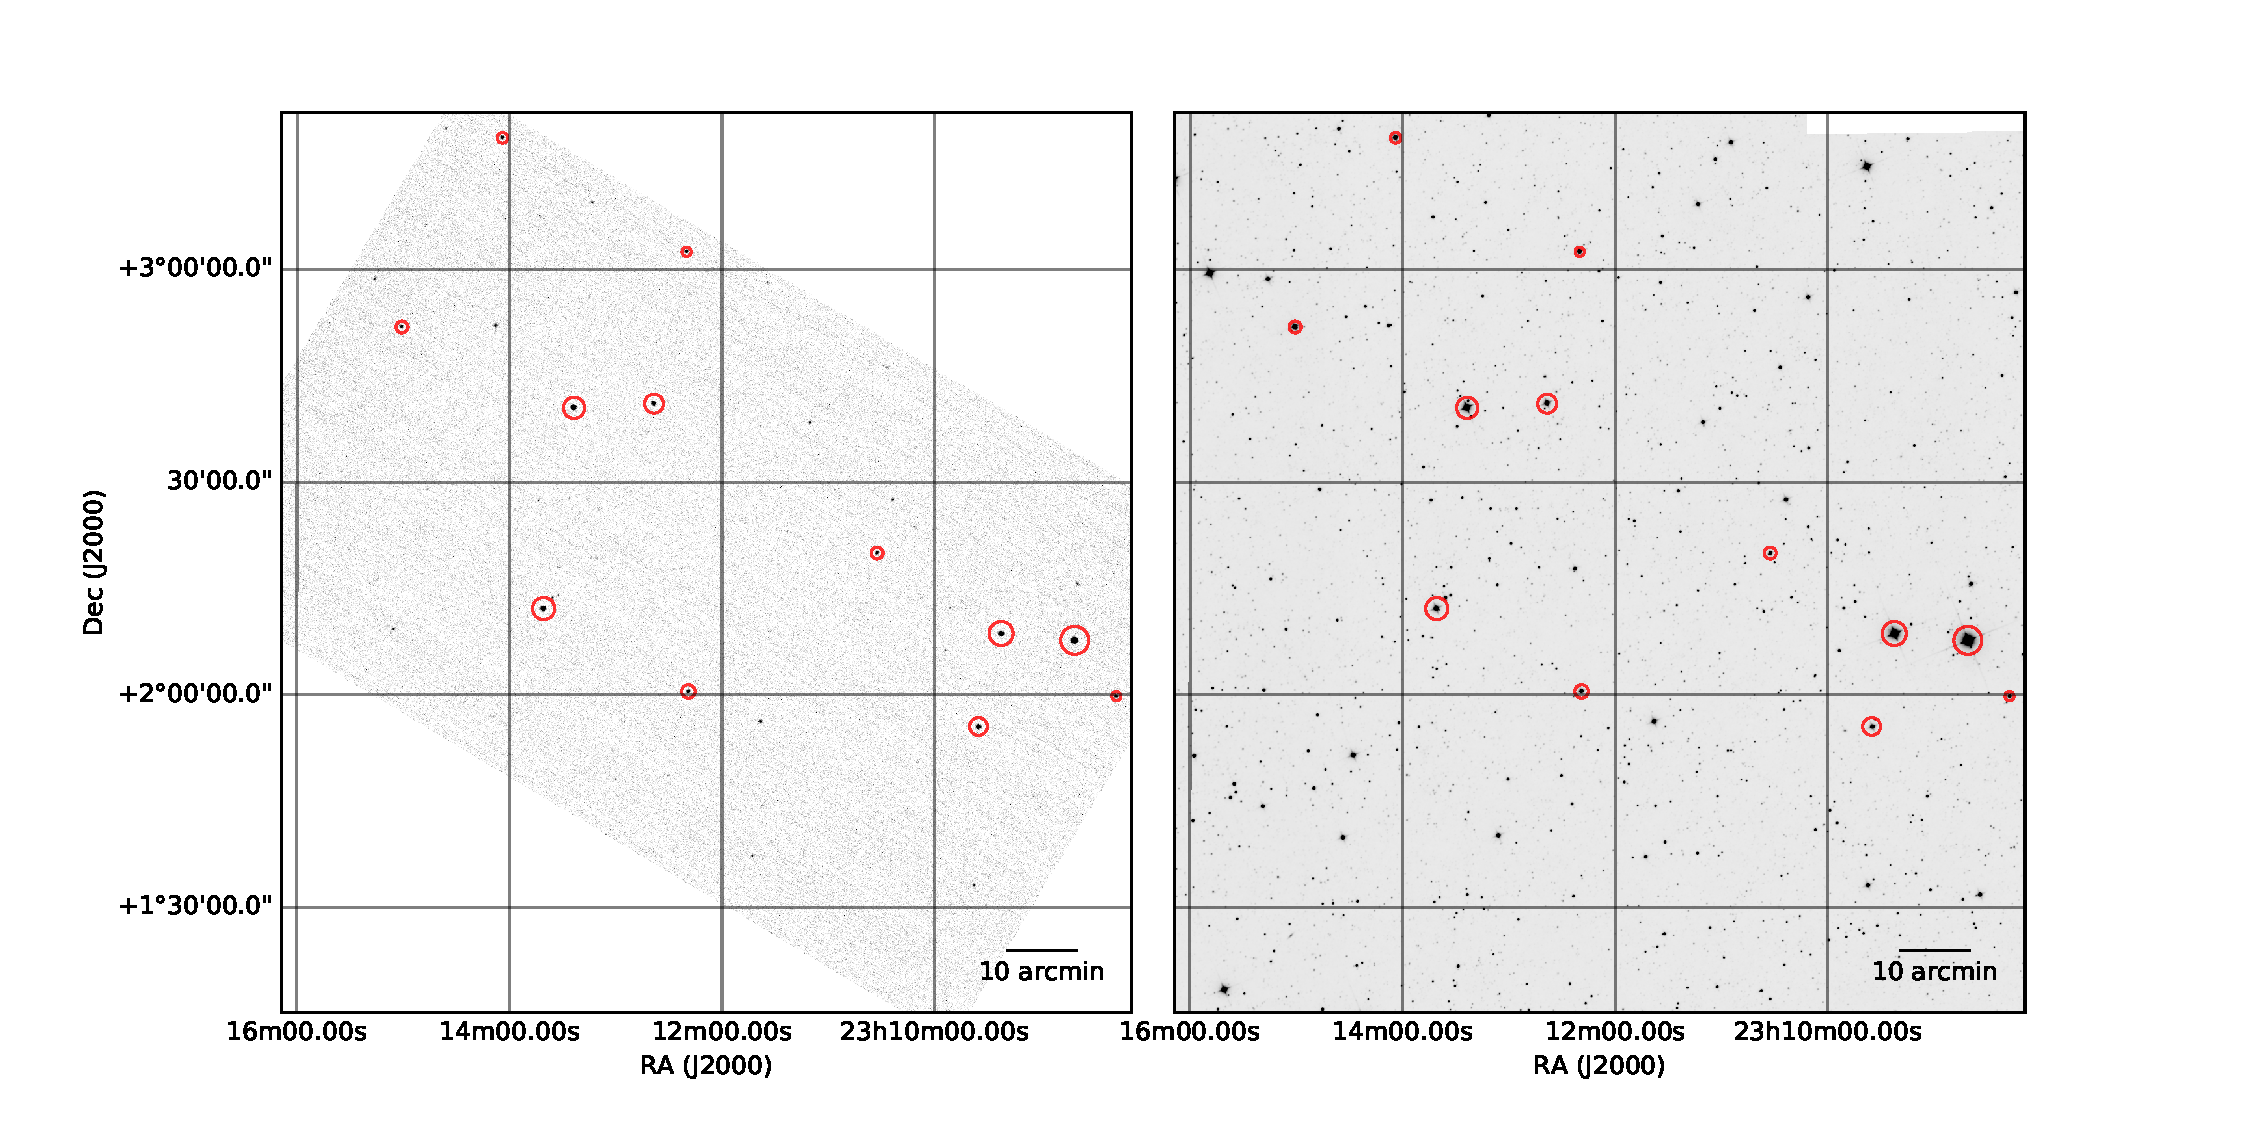
\includegraphics[width=1.5\textwidth]{Figures/starcam_images.pdf}
	\caption[Star camera example WISE]{\textit{Left}: Example of a background-subtracted star camera image with identified $>5\sigma$ sources circled in red. The orientation of the image on the celestial sphere is the one provided by BETTII's embedded star camera solver. This image corresponds to a field in the Scorpius constellation. \textit{Right}: WISE \SI{3.4}{\um} mosaic from the online archive, centered on the same location. This image is composed of 9 individual WISE images that we patched into a mosaic using the \textit{Montage}[CITE] software package.}
	\label{fig:starcamexample}
    \end{figure}
\end{landscape}
\begin{landscape}
\begin{figure}[!ht]
	\centering
	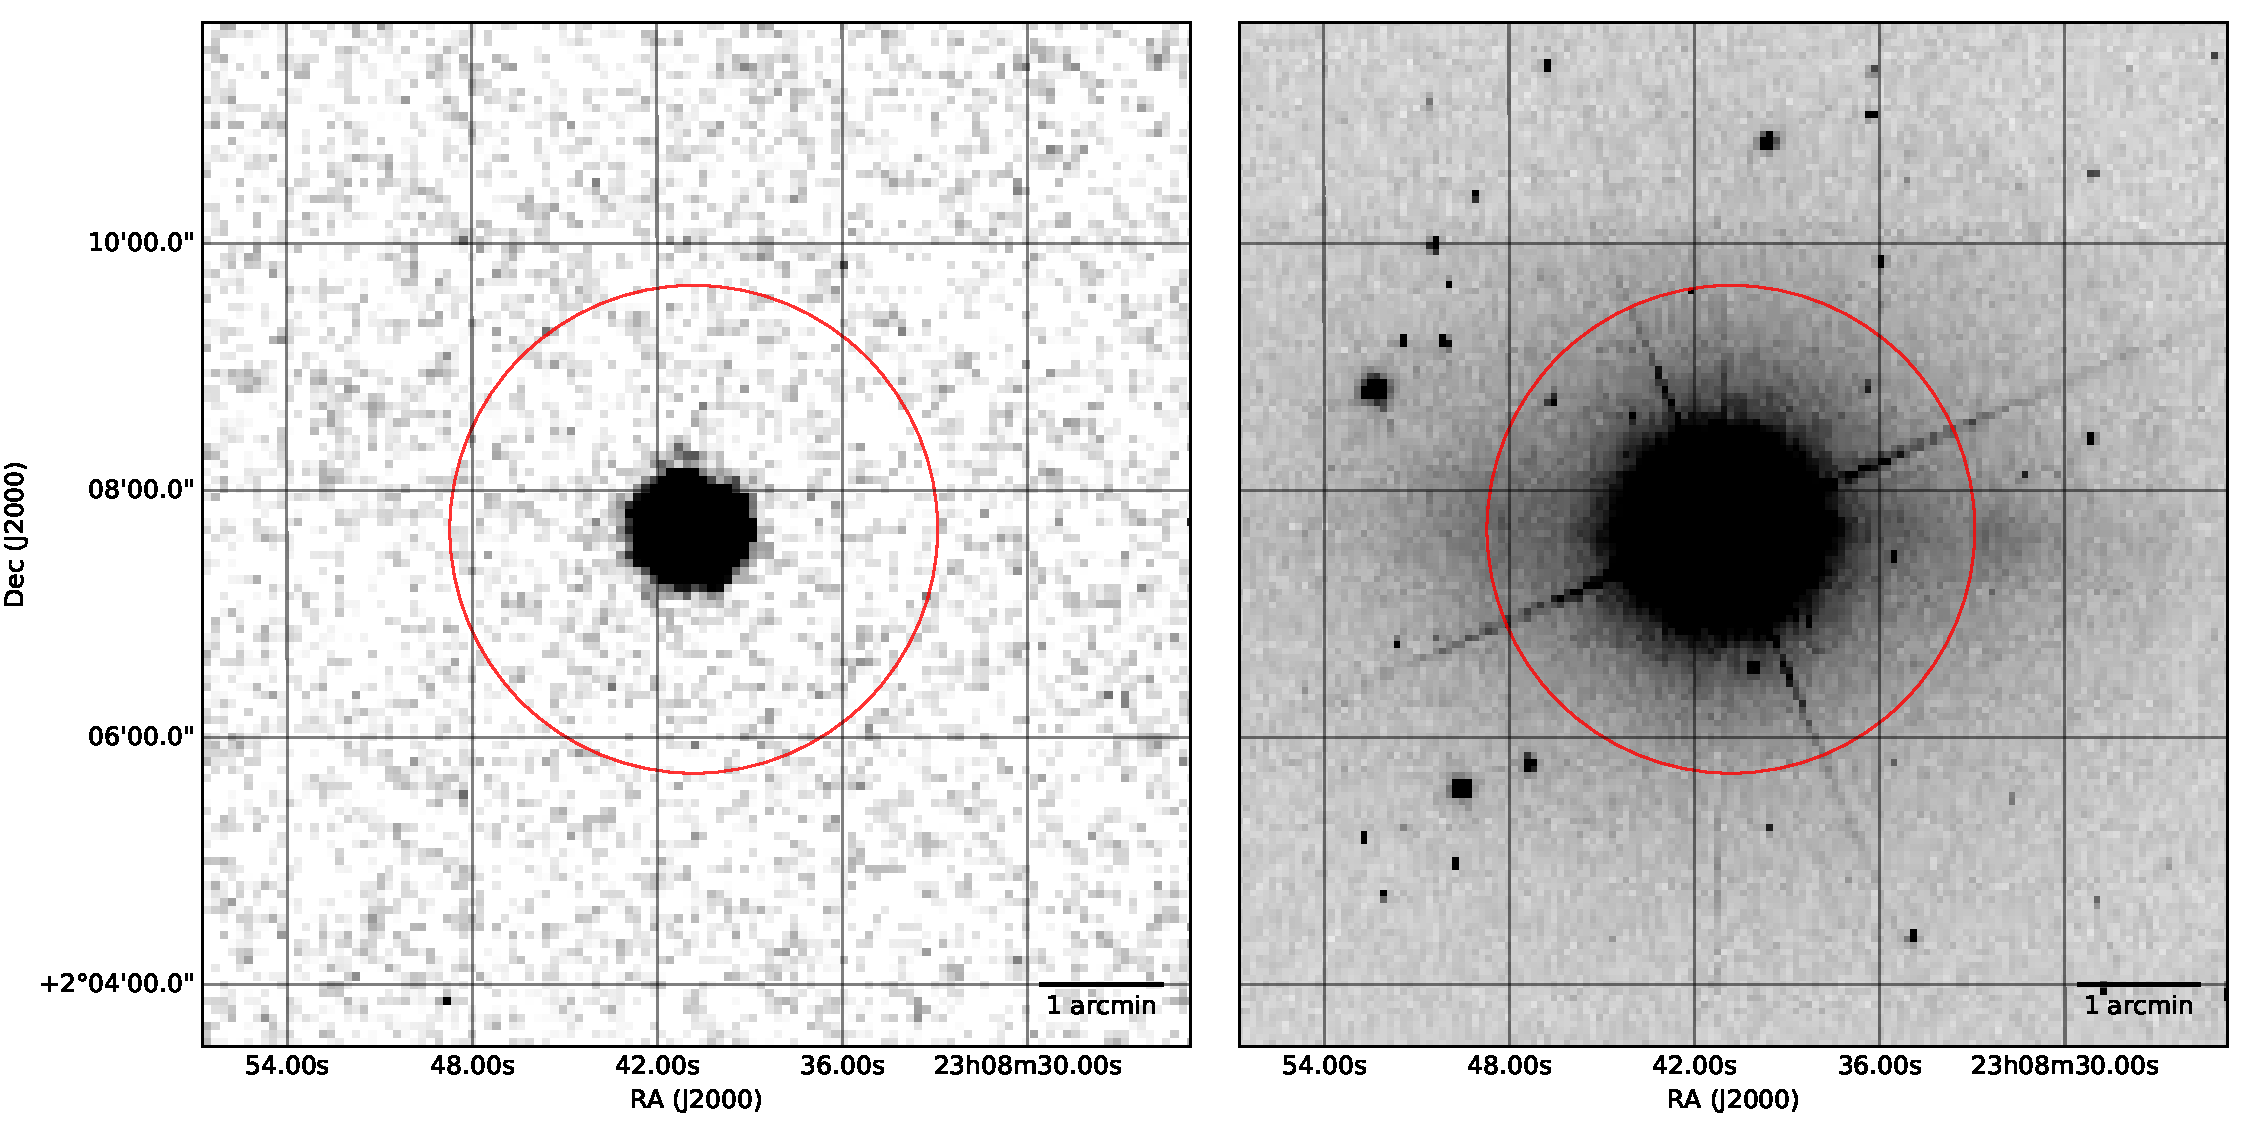
\includegraphics[width=1.5\textwidth]{Figures/starcam_SDSSr_zoom.pdf}
	\caption[Star camera individual star]{\textit{Left}: Snapshot of a bright star seen within the background-subtracted star camera frame. \textit{Right}: Snapshot taken at the same location from the WISE \SI{3.4}{\um} archive.}
	\label{fig:starcamzoom}
    \end{figure}
\end{landscape}

\paragraph{Star camera algorithm tuning}

Talk about the algorithm and its tuning: bandpass filter; field of view; new BETTII catalog;
\subsubsection{Azimuth control (CCMG)}

The CCMG features multiple encoders and motors. First, there is a brushless DC motor that spins each wheel, with a relative 13-bit encoder that monitors where the wheel is in its rotation. Second, there is a Beckhoff AS1050 stepper motor that controls the wheels' shaft angle. On the gimbal, there is a 13-bit  absolute magnetic encoder that measures the angle of the wheels from some reference. 

The motion controller that we use to monitor the wheel's speed is a brushless-DC Galil motion controller DMC-4020. It reads out the wheel encoders and controls the current to the wheels accordingly. It directly, independently implements the closed-loop system of the wheels, including all of the gains, acceleration/deceleration, and jogging speeds associated with the desired motion.

The motion controller was modified to accept an external clock pulse in order to synchronize the wheels' motion with our master clock signal. It requires a clock pulse at \SI{1.024}{\kilo\hertz}, and deviations from this value will require changing some of the gains - it is our understanding that the controller uses a \SI{1.024}{\kilo\hertz} crystal oscillator to generate it's time basis, as some of the gains and parameters to the controller can directly be entered as, for example, "steps per second". 

At power-up, the wheels immediately start accelerating to their cruising speed of \num{3000}~rpm. They take about 10 minutes to reach their target. The wheels' frequency is set for the entire duration of the flight.

The gimbal is controlled with another Galil Motion controller, a 2-axis stepper driver DMC-4020, which can also be synchronized with an external clock. Only one axis is used for the CCMG, while the second axis is used by the momentum dump motor (see section~\ref{subsec:chap3momdumpmotor}). The controller operates in micro-stepping mode and has a very smooth response, in contrast to previous controllers we tested which create a lot of vibrations. The controller is set always to use 64 micro-steps per step, and the motor is a [REFERENCE] with 200 steps per revolution. The motor is outfitted with a Beckhoff AG1000 planetary gearhead with a 3.7:1 reduction ratio. The gearbox itself has a ratio of 25, which creates a total gear ratio of 92.5. Hence, a \SI{360}{\degree} revolution of the stepper corresponds to $360/92.5=3.9^\circ$ motion of the shaft. A motion of \SI{1}{\degree} of the shaft correspond to \num{3889} motion controller steps. A motion of \SI{90}{\degree} of the shaft correspond to \num{296000} motion controller steps. Finally, the same \SI{90}{\degree} motion will translate to a \num{2048} step change in the gimbal magnetic encoder.

In practice, all of the control is done using the regular stepper motor encoder. The magnetic encoder is used for limit-checking and to feed back to the momentum dump mechanism. With this in mind, we can now relate the control signal (stepper motor micro-steps per second) to the physical torque that the wheels provide. 
\begin{eqnarray}
\Delta\theta\units{\si{\radian}} &= &\frac{2\pi}{92.5\times 200\times 64}\Delta(\textrm{micro-steps}) \\ 
& \sim & \num{5.3e-6} \Delta(\textrm{micro-steps})\\
\Delta\theta\units{\si{\arcsecond}} &\sim &  1.09 \Delta(\textrm{micro-steps})
\end{eqnarray}

At \num{3000}~rpm, the CCMG has a total stored momentum $\MCCMG= \SI{20.8}{\newton\meter\second}$. Of course, depending on the orientation of the wheels, the momentum along the $\z$ axis is only the projection of this momentum vector,
\begin{equation}
\MCCMGz\units{\si{\newton\meter\second}} = 20.8\sin\theta,
\end{equation}
where $\theta\units{\si{\radian}}$ is the angle between the horizontal axis and the rotation axis of the wheels. This makes sense: when the wheels are horizontal, there is no momentum projected on the $\z$ axis because the rotation vectors of the wheels are orthogonal to $\z$. When the rotation axes are along $\z$, we have the maximum momentum along $\z$. 

The torque is the variation of the momentum with time. So we can write:
\begin{eqnarray}
\ccmgtorque\units{\si{\newton\meter}} &= &\frac{d}{dt}\MCCMGz\\
\ccmgtorque\units{\si{\newton\meter}} &= & 20.8\times \dot{\theta}\units{\si{\radian\per\second}} \cos\theta\\
 &= & \num{1.1e-4}\times \velstepper\units{micro-step~\si{\per\second}}\cos\theta
\end{eqnarray}

\begin{figure}[!ht]
	\centering
	\includestandalone{Figures/CCMG-nocase-axes}
	\caption{}
	\label{fig:CCMGnocase}
    \end{figure}

\begin{figure}[!ht]
	\centering
	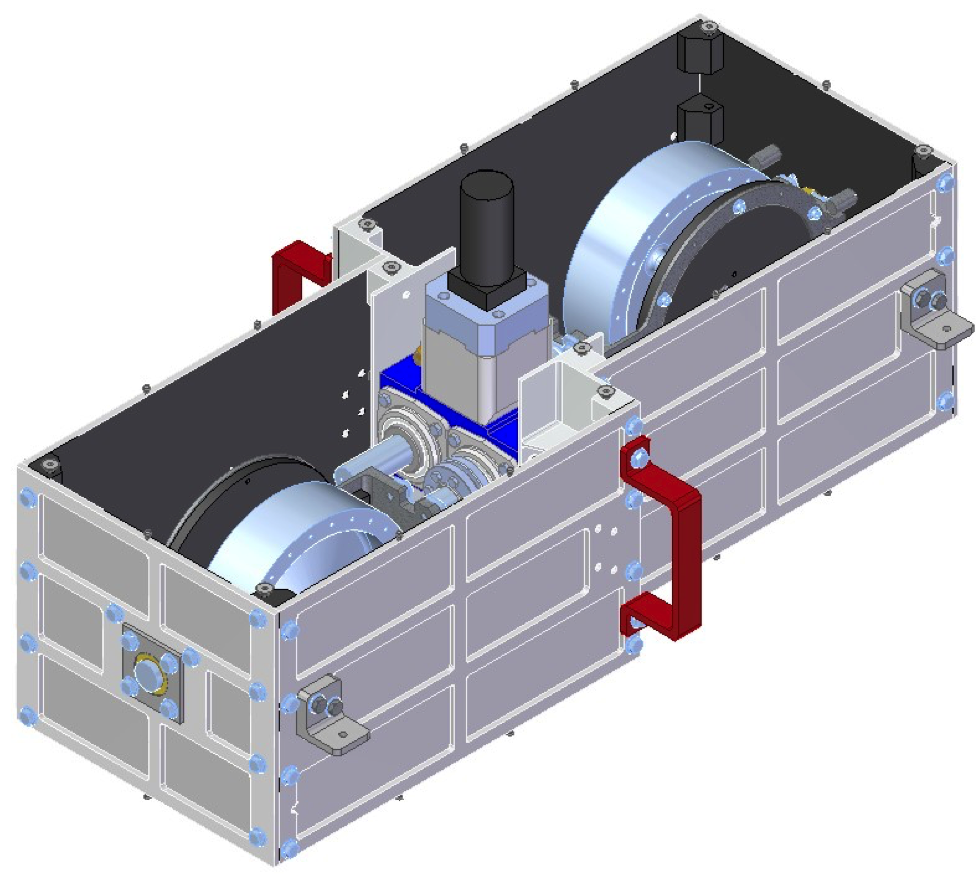
\includegraphics[width=\textwidth]{Figures/CCMG-case.png}
	\caption{}
	\label{fig:CCMGcase}
    \end{figure}


The entire CCMG assembly was tested in a vacuum chamber at cold temperatures, and operates fine. Several heaters are strategically located in the assembly to allow some thermal control for all the electronics in case issues arise.

\subsubsection{Momentum dump mechanism}
\label{subsec:chap3momdumpmotor}

The momentum management strategy consists of using the balloon as a large momentum reservoir. The control system then needs to be equipped with a system that allows a transfer of momentum between the gondola and the balloon, which are connected through the parachute and ladder. 

For this purpose, BETTII uses a design which has successfully flown on previous balloon payload (Fig.~\ref{fig:rotator}), with several improvements over its predecessors. It consists of a steel an titanium setup which will make the junction between to the bottom of the balloon train (at the very bottom of the ladder) and the very top of the gondola. The critical material is an alloy of steel that has been heat treated and is particularly strong. The setup consists essentially of a pivot and a pin made with this allow, connected together with grade 8 bolts. The top of the pin is attached to the pivot, and has a lip at the bottom on which two circular bearings are stacked: the bottom one uses ceramic balls (for their excellent friction properties and long lifetime), and the top one uses steel balls (for their excellent strength). Between the two bearings, there is a metal holder that extends all the way down below the pin. On top of the steel bearing, a titanium case sits, which attaches to the entire gondola. 

The momentum dump mechanism is a simple rotary stepper motor. Its housing attaches to the steel case of the assembly - while its shaft attaches to the metal holder between the two bearings. With an assembly like this, when a vertical upward force is exerted, the gondola's weight pushes on the bearings, which then push onto the pin's lip. When the stepper motor starts spinning, it spins only the top part of the bottom bearing, and the bottom part of the top bearing: the friction force that this exerts allows to slowly dump momentum into the pin, hence into the balloon train. 

This configuration seems dangerous since the entire weight of the payload rests on the two bearings and the pin's bottom lip, which can be hazardous during descent when the parachutes open and the payload can experience up to a 10~g vertical load. Hence, this piece of the assembly needs to be thoroughly tested and certified before launch. 

In practice, the momentum unloading happens quite slowly due to the very low friction of the bearing. As the stepper turns the bearing, it slowly turns the entire train along with the pivot for a few tens of seconds. When the train has experienced sufficient twist, it then unfurls and gives a slight kick in the opposite direction. We observed this in our data and will discuss this more in [SECTION].

[TALK ABOUT GALIL]
\begin{figure}[!ht]
	\centering
	\includestandalone{Figures/rotator}
	\caption[Momentum dump assembly]{Momentum dump assembly}
	\label{fig:rotator}
    \end{figure}

The momentum dump mechanism has not been tested in the environmental chamber - however, the stepper motor was rated for vacuum and extreme environments. One of the big unknowns is the value of the bearings' friction coefficients in the balloon environment. When powered, the stepper motor dissipates quite a large amount of heat, which will help maintain the whole assembly to a reasonable temperature. 

\begin{figure}[!ht]
	\centering
	\includestandalone{Figures/MomDumpPID}
	\caption[Momentum dump PID]{Momentum dump control loop}
	\label{fig:MomDumpPID}
    \end{figure}


\paragraph{Inertia determination}

Talk about method used to determine the inertia of the payload.

\subsubsection{Elevation control (Rotators)}

When put in terms of ground-based telescopes, BETTII is fundamentally an Alt-Az telescope: to reach a target, it has to move in azimuth, and in elevation (also called \textit{altitude}). Instead of moving the entire payload in elevation, which would have conserved the optical setup constant for all targets, we chose to move only the siderostats for increased reliability. We paid one cost: as the siderostat cover different elevations, the fields rotate on the detector, and in opposite directions. So as the elevation changes, an active compensation needs to happen, which consists of a third rotation mechanism located downstream.

These rotation mechanisms have multiple requirements: they need to operate at \SI{90}{\degree} from the gravity axis; they need to operate well at \SI{-40}{\celsius}; they need to have an inner clearance to let our \SI{2.5}{\cm} beam through; they need to be able to support many kilograms of cantilevered mass; and they need to have a precise encoder that allows not only smooth motion, but also accurate knowledge of the elevation angle. Griffin Motion LLC makes an industrial rotator that satisfies all of these conditions [Griffin picture].

These are industrial-grade brushless DC rotators. They are controlled by a three-axis Galil Motion controller DMC-4030 with sinusoidal drives. The requirement for sinusoidal drives as opposed to pulsewidth-modulated (PWM) drives stemmed from the fact that these motors were going to be \SI{5}{\meter} away from their controller at the end of each arm, and we wanted to avoid creating electromagnetic noise by having high-frequency pulses going through such a large distance. The rotary encoder is a RENISHAW RESOLUTE absolute encoder with 26 bit resolution, which corresponds to a \ang{;;0.019} angular resolution. However, the controller ignores the two bits of lowest significance, effectively giving a 24 bit resolution, corresponding to a \ang{;;0.08} angular resolution.

An old version of these rotation stages was tested in our environmental chamber, but not under load. These devices are rated to operate nominally down to \SI{-40}{\celsius}, but because of their self-heating, we do not expect that they will reach that temperature. During our cold tests of the device, we noted that the friction seemed to change, which required a re-adjustment of the PID coefficients inside the Galil controller. 

\subsubsection{Delay lines}
\subsubsection{Tip/tilt}

Our tip/tilt mechanisms are Physik Instrumente S330 piezo-electric actuators that move a flat platform in tip and tilt. We attach a mirror to that platform, and put that mirror close to a pupil of the optical system, to correct for angular errors without creating beam walk. After long discussions with the company's engineers, we ordered a custom strain gauge sensor especially tune and tested to resist low temperatures: this sensor tells the angle of the platform, which is important for our control system [see section]. Similar devices have been successfully used on sounding rocket before to provide milli-arcsecond angular control \citep{Mendillo:2012fh}. 

The piezo-electric driver electronics provide the required \SI{100}{\volt} to operate the platform, and amplify 10 times an analog 0-10~\si{\volt} command signal. Despite its broad range of motion ($\approx$~\SI{10}{\milli\radian}), they can still operate at multiple hundred of of \si{\hertz} bandwidth, even with a mirror load on top of the platform. The resonant frequency of the structure under load, which needs to be avoided at all costs to avoid severe damage, is at more than \SI{2}{\kilo\hertz}, way beyond the frequency at which we need to command the device.

The platform can be controlled in open-loop mode, where there is a simple gain between the command and the voltage applied to the piezo crystals. However, we baseline to use the closed-loop mode during flight. In this configuration, the electronics close the loop using the strain gauge sensor and the command corresponds to an angle rather than simply a voltage. The drawbacks of the closed-loop mode are a slightly decreased bandwidth and overall range of motion. In case more range is needed during flight, it is possible to switch back to open-loop mode. 


 
 
\subsubsection{Fine guidance sensor}

The fine guidance sensor is a HAWAII-1RG detector with 1024$\times$1024 pixels that is sensitive to infrared wavelengths between \SI{1}{\um} and \SI{2.5}{\um}. The device will be operated at a cryogenic temperature of \SI{77}{\kelvin}, at which the expected read noise is 18~electrons r.m.s.

\subsubsection{Clocks and timing}
Clocks and timings \\
Computers

Synchronization of the sensors and actuators are of prime importance for our payload. As an interferometer, we are extremely sensitive to vibrations which could be injected in our system by the motors. While everything was designed to maintain a very good symmetry, slight differences in the inertias or mass distribution of the reaction wheels, for example, could create a beat frequency that would be noticeable in our science data. The existence of multiple clocks, each with their own slight temperature-dependent drift, can dramatically complicate the proper retrieval of the data.

To avoid future complications, all BETTII actuators and sensors are slaved to one single \SI{50}{\mega\hertz} master clock, or an integer divider of that master clock. The cascade of the various clock dividers meets at the common value of \num{124800}, which corresponds to \SI{2496000}{\nano\second}. This is BETTII's heartbeat. Hence, \num{124800} master clock ticks correspond to the elementary cycle of all critical processes:
\begin{itemize}
\item The CDL moves of one single step
\item The H1RG reads one single frame
\item The science detector reads one single frame
\item The CCMG wheel position about its axis is checked and a correction is applied.
\end{itemize}

The advantage of this strategy can be illustrated as follows. The time it takes for a wheel to complete a revolution is set to be an integer multiple of this heartbeat, $\num{998400}=\num{124800}\times 8$ master clock ticks (about 50 revolutions per second). Hence, every 8 heartbeats, each wheel is supposed to be in the same position, and it will be controlled 8 times during one revolution to make sure it is. This completely locks in their relative velocities, on average. Let's suppose now that in their 8th position, a mechanical defects in the wheel or the bearing triggers a small vibration. This vibration will occur at a frequency which is locked with respect to our science data, such that we will see its effects every 8 data samples. In the case where these clocks are not synchronized and would unpredictably drift with respect to each other, a perturbation that occurs every 8th of a revolution has repercussions not exactly at every 8 data samples. If we think about this in the frequency domain, it means that the power peak caused by the vibration is now broadened, whereas it is very sharp in the synchronized case.

In practice, however, implementing this "single clock" approach is not straightforward for a project that has modest resources and relies heavily on commercial electronics. Most commercial motion controllers do not allow for external clock synchronization. We came up with a solution with the engineers at Galil Motion, and found a way to change their controller to accept an external TTL signal that would bypass their internal crystal oscillator at \SI{1.024}{\kilo\hertz}. The controller normally uses the internal oscillator as a definition of its time basis, so the user can send input in physical units (like acceleration or velocity) - a change in the clock frequency from the introduction of an external signal will have non-trivial repercussions.

The attitude control and sensing occurs every 4 heartbeats, which corresponds to $\approx$\SI{100.16}{\hertz}. In the rest of this discussion, we will always refer to this frequency as being at \SI{100}{\hertz} for simplicity of notation - but it important to remember that it is in fact derived from the master clock.

[PUT here the clock diagram]

\subsubsection{Computers}

BETTII will have two on-board computers (see also diagram [REF]): 
\begin{enumerate}
\item a computer which operates a real-time Linux kernel will be used to store all the date, process the up/down telemetry, acquire star camera images, solve for inertial attitude, and process the science detector and H1RG frames. This computer is named \textit{ford}.
\item an FPGA and real-time computer from National Instruments to process the sensor input/outputs, implement the attitude estimation, and synchronize all the control loops. This computer is named \textit{boop}. This is the brain of the control system. 
\end{enumerate}


\renewcommand{\arraystretch}{1.5}
\begin{table}[htbp]
\small
\begin{tabular}{c|p{12.5cm}}
\toprule
Name  & Description \& tasks  \\
\midrule\boopFPGA & 
$\bullet$ Generate \SI{50}{\mega\hertz} master clock \newline
$\bullet$ Generate all other system clocks derived from master clock\newline
$\bullet$ Trigger gyroscopes, star cameras\newline
$\bullet$ Read sensors: gyroscopes, galil controllers, \ford at \heartbeat \newline
$\bullet$ Send actuator commands at \heartbeat \newline
$\bullet$ Implement hardware protection (limit, overdrive, etc) \newline
\\
\hline
\boopRT & 
$\bullet$ Collects all sensors from \boopFPGA and estimate gondola's attitude and velocity \newline
$\bullet$ Create proper commands to all actuators and sends them to \boopFPGA  \newline
$\bullet$ Manages operating modes [REF SECTION] \newline
$\bullet$ Manages FIFOs and communication channels with \ford  \newline
\\
\hline
\ford & 
$\bullet$ Processes star camera frames to determine attitude \newline
$\bullet$ Processes science detector frames \newline
$\bullet$ Processes fine guidance sensor frames \newline
$\bullet$ Handles communication with the ground (through the CIP) and from/to \boop \newline
$\bullet$ Automatically applies observing plan if no commands from the ground: send targets to \boopRT \newline
\\
\bottomrule
\end{tabular}
\caption[BETTII embedded computers]{}
\label{tab:computers}
\end{table}

[MAKE DIAGRAM WITH ALL COMPUTERS]
\textit{ford} is an Adlink Extreme Rugged Express-IBR 3517UE with a dual-core i7 CPU and 4 GB of ECC (Error Checking and Correction) memory. The ECC memory is helpful in mitigating some of the side effects of cosmic ray hits on the memory chips. The computer has a low power consumption, which allows it to function with a simple radiator instead of a fan. 
\textit{ford} has been successfully tested at in the environmental chamber, and the temperatures of its cores under maximum CPU stress have been monitored over long periods of time. 

\textit{boop} is a National Instrument cRIO- system. It features a reprogrammable FPGA chip in addition to a dual-core real-time operating system. NI LabView is the software interface to the system. \textit{boop} will generate and distribute BETTII's master clock signal at \SI{50}{\mega\hertz}.

\subsection{Software architecture}

A diagram showing the flow of the control software is shown in Fig.~\ref{fig:ControlSystem}. 
\begin{figure}[!ht]
	\centering
	\includestandalone{Figures/SoftwareFlow}
	\caption[Software diagram]{Software layout}
	\label{fig:SoftwareFlow}
    \end{figure}


\begin{figure}[!ht]
	\centering
	\includestandalone{Figures/ControlSystem}
	\caption[Control System Design]{Control system architecture}
	\label{fig:ControlSystem}
    \end{figure}



%----------------------------------------------------------------------------------------

%\section{Attitude representation in three dimensions}
\label{sec:attituderepresentation}
%\subsection{Definitions and conventions}

There are three common representations of the orientation, or \textit{attitude}, of an object in a 3-dimensional Euclidian reference frame: in the following we will discuss the Tait-Bryan angles (which are very similar to, and sometimes confused with proper Euler angles), rotation matrices, and quaternions. All of them can be understood as a rotation of the initial reference frame $I = \{\I,\J,\K\}$ into the object's local reference frame $L = \{\i,\j,\k\}$. The reference frame $I$ is assumed to be fixed while $L$ is allowed to move. We can write each unit vector as follows: $\I = \fromto{}{I}[1,0,0]^T$, $\J = \fromto{}{I}[0,1,0]^T$, $\K = \fromto{}{I}[0,0,1]^T$, and $\i = \fromto{}{L}[1,0,0]^T$, $\j = \fromto{}{L}[0,1,0]^T$, $\k = \fromto{}{L}[0,0,1]^T$. $\{\I,\J,\K\}$ and $\{\i,\j,\k\}$ are  orthonormal bases to $I$ and $L$, respectively. The subscript before the vector indicates in which reference frame the vector is expressed, and the $T$ after the vector indicates the transpose operation. We will keep this formalism for all vectors and matrices in this work.

\subsection{Tait-Bryan/Euler angles}
\label{subsec:Tait-Bryan}
The Tait-Bryan formalism [CITE] corresponds to a sequence of three angles, each corresponding to a rotation about one of the object's main axes: these are also called "intrinsic" rotations. They differ from "extrinsic" rotation, sometimes called "Euler angles", which correspond to a rotation about one of the axes of the global (fixed) reference frame. In the following, we will focus on using exclusively intrinsic rotations, as they are more intuitive. Note that sometimes people call this formalism "Euler angles" as well, so it is important to understand how this works.
With this formalism, we start in the global reference frame and rotate the reference frame three times to end up in the 
\textit{body} reference frame, which describes the final orientation of an object. We will most often choose a well-known sequence of rotation such as the $z-y'-x''$ order, which corresponds to the angles used to describe the heading, elevation and bank of an aircraft with respect to a reference frame attached to the Earth, for example the North-East-Down reference frame. The first rotation about $\k$ will transform $I$ into $L'$. The second rotation, about the $\j$ axis of the rotated frame $L'$, transforms $L'$ into $L''$. The third and last rotation, about the $\i$ axis of $L''$, will transform $L''$ into the final orientation, $L$, of the object (see Fig.~\ref{fig:3simpleRotate}).

This sequence of rotation can be used to represent the rotation matrix that describes the attitude of an image of the sky. Celestial coordinates are usually given in terms of right ascension, declination. To fully describe the image of a patch of sky, we need another degree of freedom, which is the roll of the image about the boresight. When given these three angles: RA, DEC, and ROLL, one can reconstruct the attitude using the Tait-Bryan angles in the $z-y'-x''$ order, where the first, second and third elementary rotations correspond to the rotations in right ascension, declination and roll, respectively.

\begin{figure}[!ht]
	\centering
	\includestandalone{Figures/CelestialSphereRAandDEC2}
	\caption{}
	\label{fig:celestialSphere}
    \end{figure}
    
%     \begin{figure}[!ht]
% 	\centering
% 	\includestandalone{Figures/starCameraRefFrame}
% 	\caption{Star camera angles. The star camera reference frame as well as the telescope reference frame are represented here with the celestial sphere local RA and DEC axes in the background. There is a known matrix that transforms the star camera reference frame, where inertial attitude is measured, to the telescope reference frame, where error vectors are computed. The error vector is determined on the plane of the sky and has two projections on the telescope reference frame. The $\Delta\El=\Delta$El component corresponds to the elevation error and is corrected by the siderostat angle. The $\Delta\xEl=\Delta$xEl component corresponds to the cross-elevation error, and is corrected by the CCMG gimbal angle. Note that as the siderostat elevation is adjusted to reduce the elevation error, the transformation matrix between the star camera and telescope reference frames is adjusted as well.}
% 	\label{fig:starcamRefFrame}
%     \end{figure}

\begin{figure}[!ht]
	\centering
	\includestandalone{Figures/AzEl}
	\caption{}
	\label{fig:AzEl}
    \end{figure}


\subsection{Rotation matrices}
\label{subsec:rotationMatrices}
Perhaps the most common way to express the orientation of an object within a given reference frame is to use the matrix that describes the rotation from one reference frame to the other. Since rotations are linear transformations of $\RealNumbers^3$, there always exists a matrix to represent it. If we choose an orthonormal basis to $\RealNumbers^3$, matrices representing rotations are $3\times 3$ orthogonal matrices. When given the traditional matrix multiplication operation, $3\times 3$ orthogonal matrices with determinant of $+1$ form a group which is an isomorphism of the group of all 3-D rotations of Euclidian space (subsequently called SO(3) for "special orthogonal group") [REFERENCE?]: it means that each rotation can always be represented by exactly one $3\times 3$ orthogonal matrix. This theorem is the mathematical translation of the sometimes obvious intuition that rotation matrices always exist, are unique for a given rotation, and that the composition of two rotations is still a rotation. It also expresses the requirement that the corresponding rotation matrices have a determinant of $+1$, which can be useful when we consider numerical implementations of these matrices, as rounding errors might require a periodic normalization of the matrices to ensure they stay in this group. Note that the group of rotation is a cyclic group, since a rotation of an angle $\theta$ is the same as a rotation of $\theta+2\pi$.

We are interested in matrices describing rotations of entire coordinate systems, which are also called \textit{passive} rotations. This is different from matrices describing rotations of vectors within a given coordinate system (called \textit{active} rotations), and an important distinction that can often lead to confusion. Let's suppose that we have an initial coordinate system $I$ of basis $\{\I,\J,\K\}$, and a second coordinate system $L$ of basis $\{\i,\j,\k\}$. For example, this applies when $L$ is the body reference frame, and we want to understand its orientation with respect to an initial reference frame, such as the inertial reference frame. The basis vectors of $L$ can all be expressed by a linear combination of the basis vector of $I$. This transformation can be described using the \textit{direction cosine matrix}, which has the following expression:

\begin{equation}
\fromto{I}{L}\R = 
\begin{bmatrix}  \I\cdot\i & \J\cdot\i  & \K\cdot\i\\
                \I\cdot\j &\J\cdot\j  & \K\cdot\j \\
				\I\cdot\k & \J\cdot\k  & \K\cdot\k
\end{bmatrix}.
\end{equation}

The columns of this matrix correspond to the expression of the basis vectors of $I$ expressed in the basis of $L$. This is what we call the \textit{rotation matrix} between $I$ and $L$, and transforms vectors expressed in $I$ into their representation in $L$. With this convention, the matrix pre-multiplies the vector. For example, if we have some vector $\fromto{}{I}\vectors{u}$ expressed in the initial reference frame $I$, its expression in the reference frame $L$ will be $\fromto{}{L}\vectors{u} = \fromto{I}{L}\R \fromto{}{I}\vectors{u}$.

%Most often, a rotation matrix is defined as the matrix $\R$ that \textit{rotates} a vector from $L$ to $I$, and can be constructed by expressing the unit vectors $\i$, $\j$ and $\k$ of $L$ in the reference frame of $I$. These three vectors form the columns of the rotation matrix $\R$. So, if we construct the matrix $\R = [\fromto{}{I}\i,\fromto{}{I}\j,\fromto{}{I}\k]$, we notice that this matrix would multiply vectors expressed in the local reference frame $L$ and express them in the reference frame $I$. In the rest of this work we will always refer to $\fromto{L}{I}\R$ as this rotation matrix, where the subscript designates the starting reference frame (the reference frame in which the vectors that post-multiply the matrix will be expressed), and the superscript designates the reference frame in which the resulting vector will be expressed. 

Note that the rotation matrix $\fromto{I}{L}\R$ is an orthogonal matrix of determinant $+1$: each columns are orthogonal with each other and of unit norm. Hence, the inverse of this matrix is its transpose, which also corresponds to the rotation of a vector from frame $I$ to frame $L$: $(\fromto{I}{L}\R)^{-1} = (\fromto{I}{L}\R)^T = \fromto{L}{I}\R$.

%This convention is widespread in the literature, but can be source of confusion. A given vector can be thought of as being \textit{rotated} from one reference frame to another, as described above, which is also called an \textit{active transformation}; alternatively, one can think of the vector staying still, and the coordinate systems rotating, which is also called a \textit{passive transformation}. This is the representation that is the most useful for our purpose, and will lead to simplifications down the road, especially when this formalism is related to quaternions. 

%What is the matrix that corresponds to the \textit{passive} transformation from $I$ to $L$? In other words, what is the matrix that will pre-multiply vectors originally expressed in $I$ and express them in $L$? It is precisely the inverse (or transpose) of the matrix $\R = [\fromto{}{I}\i,\fromto{}{I}\j,\fromto{}{I}\k]$ described earlier, so that $\fromto{}{L}\vectors{u} = \fromto{I}{L}\R \fromto{}{I}\vectors{u}$. 

Let's take an example and consider the unit vector $\fromto{}{I}\vectors{u} = \fromto{}{I}(1, 0, 0)$, expressed in $I$ originally. Now, let's rotate the coordinate frame $I$ by an angle $\theta$ with respect to the axis $\k$. The new reference frame is $L' = \{\i',\j',\k'\}$. For simplification, let's consider that $\theta = +90$~degrees. It is clear that the vector $\i$ is now equal to $-\j'$, and $\fromto{}{L'}\i = \fromto{}{L'}(0,-1,0)$. 

\begin{figure}
\begin{center}
\tdplotsetmaincoords{0}{0}

%start tikz picture, and use the tdplot_main_coords style to implement the display 
%coordinate transformation provided by 3dplot
\begin{tikzpicture}[scale=4.5,tdplot_main_coords,label/.style={%
   postaction={ decorate,%transform shape,
   decoration={ markings, mark=at position .8 with \node #1;}}}]

\def\rvec{0.8}
\coordinate (O) at (0,0,0);
%draw the main coordinate system axes
\draw[line width=0.3mm,->] (0,0,0) -- (\rvec,0,0) node[below,align=left]{$\X$};
\draw[line width=0.3mm,->] (0,0,0) -- (0,\rvec,0) node[above left]{$\Y$};
\draw[line width=0.3mm] (0,0,0) -- (0,0,\rvec) node[anchor=north]{$\Z=\z'$};

\def\rotangle{30}
\tdplotsetrotatedcoords{0}{0}{\rotangle}
\draw[line width=0.3mm,->,tdplot_rotated_coords,color=blue] (0,0,0) -- (\rvec,0,0) node[below,align=left]{$\x'$};
\draw[line width=0.3mm,->,tdplot_rotated_coords,color=blue] (0,0,0) -- (0,\rvec,0) node[above left]{$\y'$};

\tdplotdrawarc[tdplot_main_coords,->]{(0,0,0)}{\rvec/3}{0}{\rotangle}{align=center,anchor=west}{$\theta$}


\end{tikzpicture}
\caption[Rotation of 30~degrees about $\Z$]{The $\{\x',\y',\z'\}$ reference frame (in blue) is rotated with respect to $\{\X,\Y,\Z\}$ (in black). The rotation is about the axis $\Z$ by an angle $\theta=30$~degrees.}
\label{fig:TopViewSimpleRotate}
\end{center}
\end{figure}

In the more general case, let's suppose that the local reference frame $L'$ is rotated by an angle $\theta$ about the $\k$ axis (Fig.~ \ref{fig:simpleRotate}) with respect to the reference frame $I$. The convention we adopt sets the rotation matrix for this transformation as being:
\begin{equation}
\fromto{I}{L'}\R = \R_\k(\theta) = 
\begin{bmatrix} \cos\theta & \sin\theta & 0 \\
				-\sin\theta & \cos\theta & 0 \\
                0 & 0 & 1
\end{bmatrix},
\end{equation}
where $\k$ indicates the third axis of the current basis ($\i$ and $\j$ represent the first and second axes, respectively). This will transform vectors from $I$ to $L'$. Suppose now that we further rotate our reference frame by an angle $\phi$ about the newly-rotated $\j'$ axis. The rotation for this elementary transformation is:
\begin{equation}
\fromto{L'}{L''}\R = \R_\j(\phi) = 
\begin{bmatrix} \cos\phi  & 0 & -\sin\phi\\
                0  & 1 & 0 \\
				\sin\phi  & 0 & \cos\phi
\end{bmatrix}.
\end{equation}
And let's do one last rotation about $\i''$, of an angle $\psi$, for which the transformation matrix is:

\begin{equation}
\fromto{L''}{L}\R = \R_\i(\psi) = 
\begin{bmatrix}  1& 0  & 0\\
                0 &\cos\psi  &  \sin\psi \\
				0 & -\sin\psi  &  \cos\psi
\end{bmatrix}.
\end{equation}

The matrix that corresponds to the active transformation of $I$ to $L$ will multiply vectors expressed in $I$ and express them in $L$. Hence, this matrix can be written:
\begin{equation}
\fromto{I}{L}\R = 
\fromto{L''}{L}\R\fromto{L'}{L''}\R\fromto{I}{L'}\R = \R_\i(\psi)\R_\j(\phi)\R_\k(\theta),
\end{equation}
where we pre-multiply the matrix for each consecutive rotation of reference frames. This corresponds to the "natural order" of rotations [CITE], and is especially relevant when related to quaternions. While the first axis of rotation, $\k$, is defined in the initial reference frame, it is important to realize that the axes corresponding to the second and third rotations are defined in the intermediate frames $L'$ and $L''$, respectively. We can understand this by thinking that the transformations follow the \textit{body}, as each rotation is done in the body reference frame, and is a particularly useful approach to our problem.


\def\rvec{0.8}
\begin{figure}
\begin{center}
\tdplotsetmaincoords{70}{110}

%start tikz picture, and use the tdplot_main_coords style to implement the display 
%coordinate transformation provided by 3dplot
\begin{tikzpicture}[scale=4.5,tdplot_main_coords,label/.style={%
   postaction={ decorate,%transform shape,
   decoration={ markings, mark=at position .8 with \node #1;}}}]


\coordinate (O) at (0,0,0);
%draw the main coordinate system axes
\draw[line width=0.3mm,->] (0,0,0) -- (\rvec,0,0) node[below,align=left]{$\X$};
\draw[line width=0.3mm,->] (0,0,0) -- (0,\rvec,0) node[above left]{$\Y$};
\draw[line width=0.3mm,->] (0,0,0) -- (0,0,\rvec) node[above] {$\K = \k'$} node[midway]{\AxisRotator[rotate=-90,->]};


\def\rotangle{-30}
\tdplotsetrotatedcoords{\rotangle}{0}{0}
\draw[line width=0.3mm,->,tdplot_rotated_coords,color=blue] (0,0,0) -- (\rvec,0,0) node[below,align=left]{$\x'$};
\draw[line width=0.3mm,->,tdplot_rotated_coords,color=blue] (0,0,0) -- (0,\rvec,0) node[above left]{$\y'$};

\tdplotdrawarc[tdplot_main_coords,->]{(0,0,0)}{\rvec/3}{0}{\rotangle}{align=center,anchor=north east}{$\theta$}


\end{tikzpicture}
\caption[Rotation of -30~degrees about $\Z$]{The $\{\x',\y',\z'\}$ reference frame (in blue) is rotated with respect to $\{\X,\Y,\Z\}$ (in black). The rotation is about the axis $\Z$ by an angle $\theta=-30$~degrees.}
\label{fig:simpleRotate}
\end{center}
\end{figure}
\begin{figure}
\begin{center}
\tdplotsetmaincoords{70}{110}

%start tikz picture, and use the tdplot_main_coords style to implement the display 
%coordinate transformation provided by 3dplot
\begin{tikzpicture}[scale=4.5,tdplot_main_coords,label/.style={%
   postaction={ decorate,%transform shape,
   decoration={ markings, mark=at position .8 with \node #1;}}}]


\coordinate (O) at (0,0,0);
%draw the main coordinate system axes
\draw[line width=0.3mm,->] (0,0,0) -- (\rvec,0,0) node[below,align=left]{$\X$};
\draw[line width=0.3mm,->] (0,0,0) -- (0,\rvec,0) node[above left]{$\Y$};
\draw[line width=0.3mm,->] (0,0,0) -- (0,0,\rvec) node[anchor=east]{$\Z=\z'$};

% first rotation about Z
\def\rotangleZ{-30}
\def\rotangleY{45}
\def\rotangleX{15}
\tdplotsetrotatedcoords{\rotangleZ}{0}{0}
\draw[line width=0.3mm,->,tdplot_rotated_coords,color=blue] (0,0,0) -- (\rvec,0,0) node[below,align=left]{$\x'$};
\draw[line width=0.3mm,->,tdplot_rotated_coords,color=blue] (0,0,0) -- (0,\rvec,0) node[below left]{$\y'=\y''$};

\tdplotdrawarc[tdplot_main_coords,->]{(0,0,0)}{\rvec/3}{0}{\rotangleZ}{align=center,anchor=north east}{$\theta$}
\tdplotsetrotatedthetaplanecoords{0}
\tdplotdrawarc[tdplot_rotated_coords,->]{(0,0,0)}{\rvec/2}{90}{90-\rotangleY}{align=center,anchor=east}{$\phi$}
%\draw[tdplot_rotated_coords,->] (\rvec/3,0,0) arc (0:90:\rvec/3);


% second rotation about y'
\tdplotsetrotatedcoords{\rotangleZ}{-\rotangleY}{0}
\draw[line width=0.3mm,->,tdplot_rotated_coords,color=red] (0,0,0) -- (\rvec,0,0) node[above,align=left]{$\x'' = \x$};
%\draw[line width=0.3mm,->,tdplot_rotated_coords,color=red] (0,0,0) -- (0,\rvec,0);
\draw[line width=0.3mm,->,tdplot_rotated_coords,color=red] (0,0,0) -- (0,0,\rvec) node[above right]{$\z''$};

\end{tikzpicture}
\caption[Two consecutive elementary rotations]{The $\{\x'',\y'',\z''\}$ reference frame (in red) is rotated with respect to $\{\x',\y',\z'\}$ (in blue). The rotation is about the axis $\y'$ by an angle $\phi=-45$~degrees.}
\label{fig:3simpleRotate}
\end{center}
\end{figure}
\begin{figure}
\begin{center}
\tdplotsetmaincoords{70}{110}

%start tikz picture, and use the tdplot_main_coords style to implement the display 
%coordinate transformation provided by 3dplot
\begin{tikzpicture}[scale=4.5,tdplot_main_coords,label/.style={%
   postaction={ decorate,%transform shape,
   decoration={ markings, mark=at position .8 with \node #1;}}}]


\coordinate (O) at (0,0,0);
%draw the main coordinate system axes
\draw[line width=0.3mm,->] (0,0,0) -- (\rvec,0,0) node[below,align=left]{$\X$};
\draw[line width=0.3mm,->] (0,0,0) -- (0,\rvec,0) node[above left]{$\Y$};
\draw[line width=0.3mm,->] (0,0,0) -- (0,0,\rvec) node[anchor=east]{$\Z=\z'$};

% first rotation about Z
\def\rotangleZ{-30}
\def\rotangleY{45}
\def\rotangleX{15}
\tdplotsetrotatedcoords{\rotangleZ}{0}{0}
\draw[line width=0.3mm,->,tdplot_rotated_coords,color=blue] (0,0,0) -- (\rvec,0,0) node[below,align=left]{$\x'$};
\draw[line width=0.3mm,->,tdplot_rotated_coords,color=blue] (0,0,0) -- (0,\rvec,0) node[below left]{$\y'=\y''$};

\tdplotdrawarc[tdplot_main_coords,->]{(0,0,0)}{\rvec/3}{0}{\rotangleZ}{align=center,anchor=north east}{$\theta$}
\tdplotsetrotatedthetaplanecoords{0}
\tdplotdrawarc[tdplot_rotated_coords,->]{(0,0,0)}{\rvec/2}{90}{90-\rotangleY}{align=center,anchor=east}{$\phi$}
%\draw[tdplot_rotated_coords,->] (\rvec/3,0,0) arc (0:90:\rvec/3);


% second rotation about y'
\tdplotsetrotatedcoords{\rotangleZ}{-\rotangleY}{0}
\draw[line width=0.3mm,->,tdplot_rotated_coords,color=red] (0,0,0) -- (\rvec,0,0) node[above,align=left]{$\x'' = \x$};
%\draw[line width=0.3mm,->,tdplot_rotated_coords,color=red] (0,0,0) -- (0,\rvec,0);
\draw[line width=0.3mm,->,tdplot_rotated_coords,color=red] (0,0,0) -- (0,0,\rvec) node[above right]{$\z''$};

% third rotation about x''
\tdplotsetrotatedcoords{\rotangleZ}{-\rotangleY+90}{\rotangleX+90}
\draw[line width=0.3mm,->,tdplot_rotated_coords,color=green] (0,0,0) -- (\rvec,0,0) node[above,align=left]{$\y$};
\draw[line width=0.3mm,->,tdplot_rotated_coords,color=green] (0,0,0) -- (0,\rvec,0) node[above left]{$\z$};
%\draw[line width=0.3mm,->,tdplot_rotated_coords,color=green] (0,0,0) -- (0,0,\rvec) ;

%\tdplotsetrotatedcoords{\rotangleZ}{-\rotangleY-90}{90+\rotangleX}
%\tdplotsetrotatedthetaplanecoords{180}
\tdplotdrawarc[tdplot_rotated_coords,->]{(0,0,0)}{2*\rvec/3}{90-\rotangleX}{90}{align=center,anchor=south}{$\psi$}


\end{tikzpicture}
\caption[Three consecutive elementary rotations]{The $\{\x,\y,\z\}$ reference frame (in green) is rotated with respect to $\{\x'',\y'',\z''\}$ (in red). The rotation is about the axis $\x''$ by an angle $\psi=15$~degrees.}
\label{fig:3simpleRotate}
\end{center}
\end{figure}


\subsection{Quaternions}
\label{subsec:Quaternions}
Quaternions are a more modern way to describe the orientation of a reference frame with respect to another, and are today widely used to describe spacecraft orientation [QUOTE]. From a strictly mathematical point of view, quaternions form a normed algebra over the real numbers that is an extension of traditional complex numbers. The quaternion normed algebra has four dimensions, instead of just two for the complex numbers. At its fundamental level, the basis for the quaternion algebra consists of one real axis and three imaginary axes \{1, $\i$, $\j$, $\k$\}. Like complex numbers (which have a basis \{1, $\i$\}), there are fundamental relations between the basis elements that govern the multiplication operation, such as the well known identity $\i^2=-1$, that we will discuss at length later in this section. In this document, we will write a quaternion using one of the following equivalent notations (Coutsias 1999) and (Schmidt 2001) :
\begin{equation}
\quat{q} = q_r\times 1 + q_i\i + q_j\j + q_r\k = q_r + \vectors{q} =
\begin{bmatrix}
q_i\\
q_j\\
q_k\\
q_r
\end{bmatrix} = \begin{bmatrix}
\vectors{q}\\
q_r
\end{bmatrix} = \begin{bmatrix}  \vectors{q}^T & q_r\end{bmatrix}^T,
\end{equation}
where we make a clear distinction between the quaternion's real part $q_r$, and its 3-dimensional imaginary part that we choose to represent as a vector $\vectors{q} =q_i\i + q_j\j + q_r\k$. Like complex numbers, quaternion have a conjugate operation, which negates the imaginary part: $\quat{q}^* = \begin{bmatrix}  -\vectors{q}^T & q_r\end{bmatrix}^T$.

Quaternions are interesting beyond their pure mathematical definition because the subset of quaternions of unit norm can be used to represent a coordinate frame rotation in three dimensions. The Euler rotation theorem states that any coordinate frame rotation can be described by a rotation of an angle $\theta$ about an appropriately-chosen unit vector $\vectors{u} = x\i + y\j + z\k$ (also called the "Euler axis" or "Euler vector"). This formalism has 3 degrees of freedom, the minimum needed to describe a rotation between two reference frames: two degrees of freedom in the vector (which is constrained to be of unit norm), and one in the rotation angle. If we encode this information in a quaternion using Euler's exponential notation for vectors [need references here], this precisely defines the quaternion:
\begin{equation}
\quat{q} = \exp\left[\frac{\theta}{2}(x\i + y\j + z\k)\right] = \cos\frac{\theta}{2} + (x\i + y\j + z\k)\sin\frac{\theta}{2}.
\end{equation}
This quaternion completely describes the rotation between the two reference frames and has unit norm. Conversely, every quaternion of unit norm can be decomposed like this and represent a rotation in three-dimensional Euclidian space. Like rotation matrices, the unit quaternions form a group under the quaternion multiplication operation, which is isomorphic to the special unitary group SU(2) [reference]. It is known that SU(2) is a surjective 2:1 homomorphism of SO(3). This means that each element in SO(3) can be described by exactly two elements in SU(2), or equivalently, two distinct unit quaternions: the quaternion $\quat{q}$, and its opposite $-\quat{q}$.

Quaternions use 4 numbers to describe 3 degrees of freedom: an advantage over matrices (9 elements), but an apparent disadvantage over Tait-Bryan angles, which consist of an optimal number of 3 elements. However, Tait-Bryan angles can be shown to exhibit a phenomenon called \textit{gimbal lock} [references], which leads to a degeneracy when describing the set of angles corresponding to rotations when the pitch angle (second rotation angle, about $\j$) is $\pm\pi/2$. This creates situations where some rotations and sequences of rotation would have to be avoided by fear of creating numerical issues caused by gimbal lock [footnote: for an example of gimbal lock, refer to the Apollo program!]. Quaternions, while needing an extra number to represent the rotation, are free of this concern. This is one of the main reasons that they were originally preferred to Tait-Bryan angles early in the spaceflight era [WERTZ 1985?]. [talk more about the advantages of quaternions: number of multiplications, etc - see Shuster et al 1993]

\subsubsection{Quaternion multiplication}

In order to form the unit quaternion group, one has to define an appropriate multiplication operation. We warn that the formulation that we use and present in the next few paragraphs does not correspond to the commonly accepted rules for quaternion operations (also called "Hamilton notation", from W. R. Hamilton who is attributed the discovery of quaternions). We use a formalism that was popularized by Caley [CITE] and adopted in most of the aerospace community [cite JPL quaternion standard], mostly to describe the orientation of satellites in inertial space. Its main advantage is that consecutive transformations using quaternions consist of multiplying elementary quaternions in a "natural order", exactly in the same order as the rotation matrices mentioned at the end of the previous section. 

[Add more philosophical dwelling on the hows and whys of this notation; including references still on page]

To avoid confusion, we will not mention the original Hamilton rules in this work. Instead, we define the quaternion elementary multiplication rules as follows[CITE]:

\begin{equation}
\label{eq:QuaternionRules}
\begin{split}
 \i^2 = \j^2 = \k^2 &= -1;\\
 \j\i = -\i\j &= \k;\\
 \k\j = -\j\k &= \i;\\
 \i\k = -\k\i &= \j.
\end{split}
\end{equation}

Using the relations in Eq.~\ref{eq:QuaternionRules}, we define the general quaternion multiplication operator $\otimes$:
\begin{equation}
\begin{split}
\quat{p}\otimes\quat{q} & =  (p_r + p_i\i + p_j\j + p_r\k)\times(q_r + q_i\i + q_j\j + q_r\k) \\
& =  (p_rq_r - p_iq_i - p_jq_j- p_kq_k)\\
& \;\;\;\;\;\; +  (p_rq_i + p_iq_r - p_jq_k + p_kq_j)\i\\
& \;\;\;\;\;\; +  (p_rq_j + p_jq_r - p_kq_i + p_iq_k)\j\\
& \;\;\;\;\;\; +  (p_rq_k + p_kq_r - p_iq_j + p_jq_i)\k\\
\end{split}.
\end{equation}

To express a vector $\fromto{}{I}\vectors{v} = \fromto{}{I}(x,y,z)$ in the new frame $L$, we construct a purely imaginary quaternion from this vector: $\quat{q}_\vectors{v} = 0 + x\i + y\j + z\k$, and we use the quaternion multiplication to obtain:
\begin{equation}
\begin{bmatrix} \fromto{}{L}\vectors{v}\\ 0 \end{bmatrix}= \fromto{I}{L}\quat{q}\otimes\quat{q}_\vectors{v}\otimes\fromto{I}{L}\quat{q}^{-1},
\end{equation} 
and extract the vector $\fromto{}{L}\vectors{v}$ from the resulting quaternion.

Note that the quaternion inverse operation for quaternions of unit norm is the same as the conjugate operation. 

\subsubsection{Relationship with matrices and elementary quaternions}
Using this formalism, a quaternion is behaving in the same way as the corresponding \textit{passive} transformation matrix to describe a reference frame rotation. This means that consecutive rotations are multiplying in the "natural order", which makes it more intuitive.

For example, let's consider the elementary rotation described in Fig~\ref{fig:simpleRotate} that represents a rotation of the initial reference frame $I$ into a reference frame $L$ about $\k$. Using the "left-hand" rule, the angle $\theta$ of rotation about $\k$ is now $\theta = +30$~degrees. This quaternion is $\fromto{I}{L}\quat{q} = \quat{q}_\k(\theta) = \cos\frac{\theta}{2} + \sin\frac{\theta}{2}\k$, and represents the same rotation as the passive rotation matrix $\R_\k(\theta)$ discussed in Section \ref{subsec:rotationMatrices}. [WORK OUT THE MATHS FOR THE VECTOR TRANSFORMATION] If the rotation of the reference frame is described by three consecutive rotations of angles $\theta$, $\phi$ and $\psi$ about $\k$, $\j'$, and $\i''$, respectively [see some figure], we can write:
\begin{equation}
\begin{split}
\fromto{I}{L}\quat{q} & =  \quat{q}_{\i}(\psi)\quat{q}_{\j}(\phi)\quat{q}_\k(\theta) \\
& = \begin{bmatrix}
0\\
\sin\frac{\psi}{2}\\
0\\
\cos\frac{\psi}{2}
\end{bmatrix}\begin{bmatrix}
0\\
0\\
\sin\frac{\phi}{2}\\
\cos\frac{\phi}{2}
\end{bmatrix}\begin{bmatrix}
0\\
0\\
\sin\frac{\theta}{2}\\
\cos\frac{\theta}{2}
\end{bmatrix}\\
\end{split},
\end{equation}
which forms a quaternion that is equivalent to the rotation matrix multiplication $ \R_\i(\psi)\R_\j(\phi)\R_\k(\theta).$
Note that the order of the quaternions is the same as the order of the matrices. This is one of the advantages of choosing this "natural order" convention [cite Shuster].


\subsection{Quaternion derivative and integration}

Properly defining the derivative and integral of quaternions is necessary for our purpose. We will need a derivative to describe our dynamic system as its orientation changes over time; and we will need to integrate (or \textit{propagate}) those equations to find a numerical solution to the attitude estimation problem.

In the following, we consider the body reference frame $L(t)$ which evolves as a function of time with respect to a fixed, inertial reference frame $I$. 

The mathematical derivations leading to those results can be found elsewhere [CITE]. Over an infinitesimal time step $dt$, the local frame is rotating by an angular vector $\delta\boldsymbol{\theta}$. The instantaneous angular velocity, expressed in the body reference frame $\L(t)$, is $\fromto{}{L(t)}\gyroVec(t) = \lim_{dt\to 0}\frac{\delta\boldsymbol{\theta}}{\delta t}$. It can be shown [CITE TRAWNY] that with this formalism, the quaternion derivative is defined using either a quaternion multiplication, or an equivalent matrix multiplication:

\begin{equation}
\fromto{I}{L(t)}\dotAttitude(t) = \frac{1}{2}\begin{bmatrix} \gyroVec \\ 0 \end{bmatrix}\otimes \fromto{I}{L(t)}\Attitude =  \frac{1}{2}\matOmega(\gyroVec)\fromto{I}{L(t)}\Attitude,
\label{eq:quaternionDerivation}
\end{equation}
where the matrix
\begin{equation}
\matOmega(\gyroVec) = 
\begin{bmatrix}
0 & \omega_z & -\omega_y & \omega_x \\
-\omega_z & 0 & \omega_x & \omega_y \\
\omega_y & -\omega_x & 0 & \omega_z \\
-\omega_x & -\omega_y & -\omega_z & 0
\end{bmatrix}
\label{eq:Omega}
\end{equation}
is going to play an important in the later sections. 

The integrator formulas are derived in []. The problem is to find a matrix $\thetaMat$ to integrate a quaternion $\fromto{I}{L(t)}\Attitude(t)$, and estimate attitude at time $t+\Deltat$, knowing the instantaneous angular velocity $\gyroVec(t)$: 
\begin{equation}
\Attitude(t+\Deltat) = \thetaMat(t,t+\Deltat)\Attitude(t)
\end{equation}
A zeroth-order solution assumes that the angular velocity $\gyroVec$ is a constant over the timestep $\Deltat$, an important special case since it describes the typical discrete representation that we will use in our software. The solution can be expressed as:

\begin{equation}
\thetaMat(t,t+\Deltat) \equiv \thetaMat(\Delta t) = \exp\left(\frac{1}{2}\matOmega(\gyroVec)\Deltat\right),
\label{eq:quaternionIntegration}
\end{equation}
where the matrix exponential is defined using a Taylor expansion [give reference for that]. 


A first-order solution is given in [TRAWNY] and uses knowledge of two previous $\gyroVec$ values to estimate the integral.

\subsection{Covariance matrices in different reference frames}
In the following, we will be describing our attitude using quaternions or rotation matrices in a Kalman filter with a state-space representation. This means that we will be make estimates of physical quantities, as well as estimates of our estimation error. These errors are represented using covariance matrices. 

Covariance matrices contain information about the cross-correlation of the variables in the state vector. The diagonal elements represent the auto-covariance of a given variable, while the terms off the diagonal indicate the degree of covariance (or correlation) between the different variables. For example, we will have three gyroscopes which will be mounted orthogonally from each other, each measuring the angular velocity about three different axes. In the ideal case, all gyroscopes are independent and the covariance matrix associated to the set of three angular velocities is diagonal, with the variances of each gyroscope on the diagonal.

If we rotate the gyroscopes' frame with a rotation matrix $\R$, the new covariance matrix $\noiseCovMat$ needs to be rotated as well: $\noiseCovMat' = \R\noiseCovMat\R^T$. 

\subsection{Small angle approximation}

Quaternions become more intuitive in the small angle approximation. Indeed, when all angles are small with respect to $\pi$, we can write:
\begin{equation}
\fromto{I}{L}\Attitude \approx \begin{bmatrix}  \frac{1}{2}\delta\boldsymbol{\theta} \\ 1 \end{bmatrix},
\end{equation}
where $\frac{1}{2}\delta\boldsymbol{\theta} = \frac{1}{2}[\delta\theta_i,  \delta\theta_j, \delta\theta_k]^T$ corresponds to three small rotations about all the three axes of the initial reference frame. Because we are in the small angle approximation, the order of the rotations does not matter. Hence, if the imaginary part of a quaternion has small values $q_i, q_j, q_k$, and if $q_r\approx 1$, this quaternion represents a rotation of the reference frame by an angle $\delta\theta_i = 2q_i$, then by an angle $\delta\theta_j = 2q_j$, and finally by an angle $\delta\theta_k = 2q_k$, where all the angles are expressed in radians.

More simplifications can also be found. For example, in the limit where $\gyroVec \to \boldsymbol{0}$, the matrix exponential defined in Eq.~\ref{eq:quaternionIntegration} simplifies into:
\begin{equation}
\thetaMat(\Deltat) \stackrel{\gyroVec \to \boldsymbol{0}}{=} \I_{4\times 4} + \frac{\Deltat}{2}\matOmega(\gyroVec).
\label{eq:quaternionIntegrationSimple}
\end{equation}



%\subsection{Examples} (believe me, examples are very very important when people read your stuff – if only other people had put examples in their write-ups!)
%\subsection{Implementation in software}
%As part of this effort, we wrote quaternion libraries in C++, Python, and Labview. In all cases, we use double floating point representation for the quaternion and its associated operations, to ensure that we do not lose information due to numerical round-off errors. Indeed


%----------------------------------------------------------------------------------------

\section{3D attitude estimation and sensor fusion}
\label{sec:KalmanFilter}
\renewcommand*{\arraystretch}{0.75}


The attitude estimation consists of combining high-frequency angular velocity measurements of the payload with low-frequency attitude measurements. The high-frequency measurements, usually from gyroscopes, are relative measurements, and exhibit biases and noise. The attitude measurements are absolute, but they are usually very noisy. The Kalman filter combines these two measurements in a mathematical formalism that uses the physical relationship between them. The goal of the filter is to estimate the bias of the high-frequency measurements, hence providing bias-corrected, trustworthy dynamical information that can be used to estimate the attitude at all times, even when there is no absolute measurement.

In our situation, gyroscopes will provide high-frequency velocity data (typically at 100~Hz), while star cameras will provide absolute measurements every few seconds. The gyroscopes are much more trustworthy over short periods, so they won't be influenced by just a few star camera measurements. However, on long timescales, the attitude as propagated using the gyroscopes will drift with respect of the star cameras because of the gyroscopes' inherent biases. The Kalman filter will estimate those biases and provide a bias-corrected angular velocity to make sure that the gyroscopes do not drift away from the star camera results.

This filter is very common for spacecraft attitude and control, although a large number of variations exist. It was first popularized in the 60's [CITE KALMAN original paper?] in the United States during the Apollo missions [reference], when it was used to determine the attitude of the Apollo capsules in inertial space. 

[Some paragraph on the theory of the Kalman filter: the fact that it is the optimal filter for gaussian stochastic processes, which means it converges the fastest.]

[Talk about references on Kalman filter. REcent pub: \citep{Crassidis:2011ud},\citep{Markley:2014dn}]

One of the complications of the Kalman filter is that it involves inverting matrices to find the optimal solution when new absolute measurements are received. This has implications in terms of numerical complexity which often will limit the bandwidth of the filter, especially in the context of resource-limit FPGA computers on spacecraft. In practice the trade-off is the following: either limit the bandwidth of the filter, or limit the number of state parameters (\textit{i.e.} limit the rank of the matrix to invert). Fortunately, on the ground, this limitation is usually not an issue. We will be flying a very powerful FPGA computer on our balloon, so we also will not be limited by numerical complexity.

In order to set up the Kalman filter, we choose quaternions to describe our attitude, for the reasons explained in the earlier sections and their advantages in representing all the required information efficiently. In addition, because of their nice behaviour when it comes to small angles, we can use quaternions in their linear, small angle approximation to create a \textit{multiplicative}, \textit{extended} Kalman filter (MEKF) \citep{Lefferts:1982dx}. It is extended because it operates in the small angle approximation, hence it is a local approximation of a non-linear relationship. And it is multiplicative, instead of being additive, because we use the quaternion multiplication operation to describe the "difference" or error between two reference frames. One popular instance where this filter was successfully implemented was on board the WMAP spacecraft [CITE].

First, we need to choose a representation for our sensor suite: the gyroscopes and the star cameras. Second, we describe the equations that govern the physics of our system and connect the sensors together: this is critical for the Kalman filter to produce robust estimates, and the more accurate our representation is, the more accurate our predictions can be. Finally, we discuss the Kalman setup, and two phases of the algorithm: prediction and update.

\subsection{Sensor models}
\label{sec:SensorModels}
\subsubsection{Gyroscope model}

The gyroscope model that we use is: $\gyroVecMeas  =  \gyroVec + \bias + \nGyros$, where $\gyroVecMeas$ is the measured angular velocity vector, $\gyroVec$ is the true angular velocity vector, $\bias$ is the bias vector, and $\nGyros$ is the angular velocity noise vector (also called the "rate noise"). We consider that $\nGyros$ is a white noise process with a diagonal covariance matrix $\N_\gyro = \sigma_{c,\gyro}^2\bI_{3\times 3}$. 

We consider that the derivative of the bias $\bias$ is also a white noise process: $\dot{\bias} = \nBias$, where $\nBias$ has a diagonal covariance matrix $\N_\bias = \sigma_{c,b}^2\bI_{3\times 3}$.

Assuming that the covariance matrices are diagonal help to set up the filter, but is not a necessary assumption in the general case. The following implementation is not relying on this assumption.

%The angular random walk of the gyroscope assemblies is 0.2~deg.sec$^{-1}$ with an effective bandwidth of 50~Hz (100~Hz sampling). 

The angular random walk (ARW) specification from the manufacturer is ARW = \SI{5e-4}{\deg\per\hour}. This means that if we integrate the gyroscope's rate for 1~hour, the $1\sigma$ uncertainty on our position would be 
$\SI{5e-4}{\deg}\sim\ang{;;1.8}$. For an integration time of 1 second, it would be \ang{;;0.03}. For a single integration time step $\Deltat = \SI{0.01}{\second}$, it would be \ang{;;0.003}. 

The units required for $\sigma_\gyro$ are [\si{\radian\raiseto{-0.5}\second}], so we convert:
\begin{equations}
\sigma_\gyro\units{\si{\radian\raiseto{-0.5}\second}} = \frac{\pi}{60\times180}\times \textrm{ARW}\units{\si{\deg\raiseto{-0.5}\hour}} \sim 1.5\times 10^{-7}~\si{\radian\raiseto{-0.5}\second}.
\end{equations}

Note that we can relate the ARW to the measured discrete rate noise uncertainty $\sigma(\nGyros^\textrm{meas})$ with:
\begin{equations}
\sigma(\nGyros^\textrm{meas})\units{\si{\deg\per\second}} = \textrm{ARW}\units{\si{\deg\raiseto{-0.5}\hour}}\times 60\sqrt{\textrm{BW}\units{\si{\hertz}}}
\end{equations}
where $\textrm{BW}\units{\si{\hertz}}$ is the gyroscope's bandwidth, equal to \SI{50}{\hertz} for our system. We obtain a quantity close to the measured quantity, $\sigma(\nGyros^\textrm{meas})\sim\SI{0.2}{\arcsec\per\second}$.

The bias instability units are [\si{\radian\raiseto{-3/2}\second}]. The manufacturer specification gives a maximum bias instability over a wide range of temperatures equal to \SI{0.005}{\deg\per\hour}. This is for a bandwidth of \SI{50}{\hertz}, so we obtain the bias instability term, which also corresponds to the process noise of our Kalman filter:
\begin{equations}
\sigma_\bias\units{\si{\radian\raiseto{-3/2}\second}} = \SI{0.005}{\deg\per\hour}\times \sqrt{\textrm{BW}\units{\si{\hertz}}}  \sim \SI{1.8e-7}{\radian\raiseto{-3/2}\second}.
\end{equations}
This represents how much what we are trying to estimate is expected to vary. The drift is extremely slow for our gyroscopes, so in practice we will be dominated by the changes in the alignment of the system for all relevant timescales before the gyroscope bias becomes a problem.

\subsubsection{Star camera model}

The star camera takes a picture of the sky to make noisy measurements of the right ascension (RA) and declination (DEC) of the boresight, as well as the roll angle (ROLL) in which the frame is taken. The RA and DEC typically are much more accurate than the roll angle. Each angle is can be used as en Euler angle to define the attitude of the payload in the inertial frame (or equivalently, the rotation from the inertial frame to the current attitude). Each angle corresponds to a quaternion rotation about a single axis: 
\begin{eqnarrays}
\quat{q}_\textrm{RA} &=& [0, 0, \sin(\textrm{RA}/2),\cos(\textrm{RA}/2)]^T,\\
\quat{q}_\textrm{DEC} &=& [ 0, \sin(\textrm{DEC}/2), 0,\cos(\textrm{DEC}/2)]^T,\\
\quat{q}_\textrm{ROLL}& = &[  \sin(\textrm{ROLL}/2),0,0,\cos(\textrm{ROLL}/2)]^T,\\
\Attitude^{\textrm{meas}}_{\starcam}& = &\quat{q}_\textrm{ROLL}\quat{q}_\textrm{DEC}\quat{q}_\textrm{RA}.
\end{eqnarrays}

The errors associated with the three Euler angles are assumed to be a random vector $\nStarcam$, also with a diagonal covariance matrix $\measCovMat$. [MENTION TYPICAL STAR CAMERA NOISES]

The star camera is often oriented at a fixed position on the payload, which is not necessarily aligned with the gyroscope reference frame. In that case, the attitude quaternion needs to be rotated by the quaternion representing the transformation between both reference frames. In addition, the covariance matrix needs to be rotated by the direction cosine matrix corresponding to the same transformation. This would not have an effect if the covariance matrix was a multiple of the identity matrix, but it usually is not the case since the Roll measurement is often much less sensitive. This can have implications while designing the balloon payload and deciding on the placement and orientation of the star camera: the attitude estimation will be less precise about the Roll axis of the star camera.

%The fundamental problem is trying to determine the attitude of the payload in the inertial reference frame, using biased gyroscope measurements at high frequency and absolute star camera measurements at low frequency. 

% \subsection{[PUT THIS IN APPENDIX?] Tools required for the Kalman Filter}
% \subsubsection{Quaternion propagation}
% \subsubsection{Quaternion operations}



\subsection{Continuous state equation and error}

We want to use the Kalman filter to obtain an estimate of the attitude quaternion $\Attitude_k \equiv \fromto{I}{G}\Attitude(t)$, but also use it to estimate the gyroscope biases $\bias(t)$ to improve overall performance. The "state" of our system is described by the vector:
\begin{equations}
\stateVec(t) = \begin{bmatrix} \fromto{I}{G}\Attitude(t) \\ \bias(t) \end{bmatrix}.
\end{equations}

The evolution of the state is governed by the two differential equations that follow:
\begin{eqnarrays}
\fromto{I}{G}\dotAttitude(t) & = &\frac{1}{2}\matOmega(\gyroVec(t))\fromto{I}{G}\Attitude(t),\\
\dot{\bias}(t) & = & \nBias(t),
\end{eqnarrays}
with $\gyroVec = \gyroVecMeas - \bias - \nGyros$. These equations represent the exact relationship between our quantities of interest, assuming that the noise values are known. In practice, we will create an \textit{estimator} that is used to evaluate the expected value of these quantities. This estimator, $\EstStateVec = \left[\EstAttitude(t) , \EstBias(t)\right]^T$, is governed by the following equations:
\begin{eqnarrays}
\fromto{I}{G}\dotEstAttitude(t) & = &\frac{1}{2}\matOmega(\EstGyroVec(t))\fromto{I}{G}\EstAttitude(t),\\
\dot{\EstBias}(t) & = & \boldsymbol{0},
\end{eqnarrays}



%\subsection{Error state representation}
%The state $\stateVec$ has 7 components, but it is numerically more stable to reduce it to 6 by using the unity constraint within the attitude quaternion. It is also possible to linearize the system using the error representation of the state. In this representation, our model is the difference between the true and estimated state. Since we use a quaternion representation for the attitude, it is convenient to express this difference in a multiplicative form:

The Kalman filter's goal is to minimize the variance of the estimator's error - that is, of the error vector $\stateVec-\EstStateVec$. However, in our case, we have constraints in the system since we force the quaternion to be of unit length: this introduces a singularity in the covariance matrix  of the error vector, and is prone to numerical complications. It is possible to circumvent this problem by using the multiplicative properties of the quaternion used in the small angle approximation. This is called a "multiplicative" Kalman filter, as opposed to a more traditional "additive" filter.

To do this, instead of following the evolution of the state $\EstStateVec$ itself, we will follow the evolution of the error vector $\ErrorState = [\deltaTheta,\deltaBias]^T$, where $\deltaTheta$ corresponds to the 3-dimensional angular error between true and estimate attitude quaternion taken from the difference quaternion $\fromto{\hat{G}}{G}\delta\Attitude = \fromto{I}{G}\Attitude\otimes\fromto{I}{\hat{G}}\EstAttitude^{-1} \approx [1,\frac{1}{2}\deltaTheta]^T$, and $\deltaBias = \bias - \EstBias$. 

The evolution $\EstStateVec$ as a function of time can be obtained by taking the quaternion derivative of the true attitude quaternion $\dotAttitude = \dot{\delta\Attitude} \otimes \EstAttitude + \delta\Attitude \otimes \dotEstAttitude$. With our gyroscope model, we can write:
\begin{eqnarrays}
\gyroVecMeas & = & \gyroVec + \bias + \nGyros,\\
 \EstGyroVec & = & \gyroVecMeas - \EstBias, \\
\textrm{so} \quad \gyroVec & = & \EstGyroVec - \nGyros - \deltaBias.
\end{eqnarrays}


% Traditionally, the Kalman filter uses a state, $\stateVec$, and tries to minim
% In order to define the Kalman filter, we need to understand the errorThe state $\stateVec$ has 7 components
% \begin{equations}
% \fromto{I}{G}\Attitude = \fromto{\hat{G}}{G}\delta\Attitude \otimes\fromto{I}{\hat{G}}\EstAttitude.
% \end{equations}
% For small angle approximations, we can write $\fromto{\hat{G}}{G}\delta\Attitude \approx [1,\frac{1}{2}\deltaTheta]^T$. $\deltaTheta_k$ represents the vector of angles that represent the rotation between the estimated and true reference frame in the angle-axis representation, and is expressed in the gyroscope reference frame.
% Similarly, we define $\deltaBias = \bias - \EstBias$, and form the 6-dimension error state representation $\ErrorState = [\deltaTheta,\deltaBias]^T$. It is now important to establish which equations govern this error state in order to understand the expected evolution of the system.

After a lengthy derivation to express $\dot{\deltaTheta}$ from $\dot{\delta\Attitude} = [0, \frac{1}{2}\dot{\deltaTheta}]^T$ \citep{Trawny:2005va}, we obtain:
\begin{equations}
\dot{\deltaTheta} = -\EstGyroVec\times\deltaTheta - \deltaBias - \nGyros.
\end{equations}
Note that the cross-product $\EstGyroVec\times\deltaTheta$ is equal to the matrix multiplication $\omegaCross\deltaTheta$.

The bias equation is: 
\begin{equations}
\dot{\deltaBias} = \dot{\bias} - \dot{\EstBias} = \nBias.
\end{equations}
The equations representing the evolution of the error $\ErrorState$ are then:
\begin{equations}
\dot{\ErrorState} = \begin{bmatrix} \dot{\deltaTheta} \\ \dot{\deltaBias} \end{bmatrix} = \Fc \begin{bmatrix} \deltaTheta \\ \deltaBias\end{bmatrix} + \Gc \begin{bmatrix} \nGyros \\ \nBias \end{bmatrix},
\end{equations}
with
\begin{equations}
\Fc = \begin{bmatrix} \omegaCross & -\bI_{3\times 3} \\ \bzero_{3\times 3} & \bzero_{3\times 3} \end{bmatrix},
\end{equations}
and:
\begin{equations}
\Gc = \begin{bmatrix} -\bI_{3\times 3} & \bzero_{3\times 3} \\ \bzero_{3\times 3} & \bI_{3\times 3} \end{bmatrix}.
\end{equations}

Using this error representation allows us to fully describe the state error covariance matrix that will be minimized during the Kalman filter steps. 

%\renewcommand*{\arraystretch}{0.75}
It is important here to introduce the expression of the covariance matrix of this continuous representation. Writing the noise vector $\vectors{n} = \begin{bmatrix} \nGyros \\ \nBias \end{bmatrix}$, the covariance matrix is the expected value of the product of two noise vectors taken at different times [cite TRAWNY]:
\begin{equations}
\noiseCovMat_c = E[\vectors{n}(t+\tau)\vectors{n}^T(t)] = 
\begin{bmatrix} \sigma_{c,\gyro}^2\bI_{3\times 3} & \bzero_{3\times 3}\\ \bzero_{3\times 3} & \sigma_{c,b}^2\bI_{3\times 3}\end{bmatrix}
\end{equations}

\subsection{Integration of continuous equations}

Since our system has a fast sampling rate compared to the characteristic times of the system, we consider that $\boldsymbol{F}_c$ is constant over a time step. This helps the integration of the state equation between $t_{k-1}$ and $t_k=t_{k-1}+\Deltat$, which has a discrete state transition matrix $\StateTransitionMat_k$:
\begin{equations}
\StateTransitionMat_k = \StateTransitionMat(t_k, t_{k-1}) = \exp\left(\Fc\Delta t\right) \equiv \begin{bmatrix} \boldsymbol{\Theta_k} & \boldsymbol{\Psi_k} \\ \bzero_{3\times 3} & \bI_{3\times 3}\end{bmatrix},
\end{equations}
with $\boldsymbol{\Theta_k} \sim \bI_{3\times 3} - \Deltat\omegaCross + \frac{\Deltat^2}{2}\omegaCross^2$ and $\boldsymbol{\Psi_k} \sim \bI_{3\times 3}\Deltat +  \frac{\Deltat^2}{2}\omegaCross - \frac{\Deltat^3}{6}\omegaCross^2$, where omitted the $k$ subscript to $\EstStateVec$ for clarity.

These expressions are now what we need to establish a discrete version of the state equations, which are based on this transition matrix $\StateTransitionMat_k$.

\subsection{Discrete covariance matrices}
Since we have a discrete system, it is necessary to also represent the covariance matrix discretely. The discrete system covariance matrix $\noiseCovMat$ sampled between time $t_k$ and $t_{k+1} =t_{k}+\Deltat$ is related to the continuous matrix $\noiseCovMat_c$ through the complicated relationship \citep{Maybeck:1982vh}:
$$
\displaystyle\noiseCovMat = \int^{t_{k+1}}_{t_k} \StateTransitionMat(t_{k+1},\tau)\Gc(\tau)\noiseCovMat_c\Gc^T(\tau)\StateTransitionMat^T(t_{k+1},\tau)d\tau.
$$
The full result of this equation is given in \citep{Trawny:2005va}. To the second order in $\Deltat$, the equations simplify when $\gyroVec\to \boldsymbol{0}$:
\begin{eqnarrays}
\noiseCovMat_{11} &=& \sigma_\gyro^2\Deltat\cdot\bI_{3\times 3}\\
\noiseCovMat_{12} &=& -\sigma_\bias^2\frac{\Deltat^2}{2}\cdot\bI_{3\times 3}\\
\noiseCovMat_{22} &=& \sigma_\bias^2\Deltat\cdot\bI_{3\times 3},
\end{eqnarrays}
with 
\begin{equations}
\noiseCovMat = \begin{bmatrix} \noiseCovMat_{11} & \noiseCovMat_{12} \\ \noiseCovMat_{12}^T & \noiseCovMat_{22}\end{bmatrix}.
\end{equations}
\subsection{Discrete Kalman filter setup}
%A truth model is a description of how the true state evolves physically. While the state representation can be given in continuous terms, here we immediately use a discrete approach. We have:
The Kalman filter will estimate the current attitude quaternion and gyroscope bias value, while minimizing the covariance of the error $\ErrorState$. Let's summarize the relevant physical equations that are used to set up this filter. This is useful if one wants to build a physical model of the dynamic system.
\begin{enumerate}
\item \textbf{Velocity estimate}: $\EstGyroVec_{k} = \gyroVec_k^{\textrm{meas}} - \EstBias_{k}$,
\item \textbf{Attitude propagation}: $\EstAttitude_{k} = \exp\left(\frac{1}{2}\matOmega(\EstGyroVec_{k})\Deltat\right)\EstAttitude_{k-1},$
\item \textbf{State error evolution}: $\ErrorState_{k}  = \StateTransitionMat_{k}\ErrorState_{k-1} + \boldsymbol{G}_{k}\vectors{n}_{k}$,
\item \textbf{Error covariance to be minimized}: $\stateCovMat_{k} = \cov{\ErrorState_{k}}$,
\item \textbf{Error covariance evolution}: $\stateCovMat_{k}  =   \StateTransitionMat_k \stateCovMat_{k-1}\StateTransitionMat^T_k + \noiseCovMat_k$
\item \textbf{New attitude measurement}: $\Attitude^{\textrm{meas}}_k$, 
\item \textbf{State error measurement}: $\zMeasurement_k = \measErrMat_k\ErrorState_k + \nMeas_k$. 
\end{enumerate}

Note that in that last step, the error measurement $\zMeasurement_k$ is determined by extracting $\deltaTheta_k^{\textrm{meas}}$ from the difference quaternion $\delta\Attitude_k = \Attitude^{\textrm{meas}}_k \otimes \EstAttitude^{-1}_{k}$ using the small angle approximation. Furthermore, we have $\vectors{n}_k = \begin{bmatrix} \nGyros & \nBias \end{bmatrix}^T$, $\nMeas_k$ is the measurement noise, and in our case $\measErrMat_k = \begin{bmatrix} \bI_{3\times 3} & \bzero_{3\times 3} \end{bmatrix}$.

At each step, we will attempt to produce our best estimate of the state $\EstStateVec$, and keep track of the evolution of the state error $\ErrorState$ and its covariance matrix $\stateCovMat$. There are two distinct phases in the Kalman filter: the prediction, and the update.

In the prediction phase, we use our best estimates from the previous step, along with the velocity measurements and the expected propagation relationships to predict what the estimates should be at the current step. If we don't get a new attitude measurement at that step, then these new estimates are the best we can do.

When we do get a new attitude measurement, then in addition to the prediction phase, we also do an update phase. We compare the best estimate from the prediction phase to our new measurement, and use the difference to compute a correction to our state. This uses the weights of the various noise contributors in the system, as we discuss in section []. This phase most importantly estimates the bias of the gyroscopes, to allow robust propagation of the state from one step to the next.

For our application, update phases are rare since the star camera can take hundreds of loop cycles to produce an attitude solution. Hence, the last measured star camera occurred at step $k-N$. Until we receive a new measurement, we are trusting our gyroscope model and our bias estimate to propagate the attitude correctly.

In this section, we will assume that the attitude measured by the star camera $\Attitude^{\textrm{meas}}_k$ corresponds to the attitude at the current step. In reality, when we receive the star camera, it represents an attitude that was taken some number of steps ago. This is due to the slow processing of the star camera images and the catalog search. Our software cannot solve the star camera position in one single loop iteration. We tackle this issue in section []. 

\subsection{Kalman filter: prediction}

% The Kalman filter propagation equations for the state error can be written:
% \begin{eqnarrays}
% \ErrorState_{k|k-N} & = & \StateTransitionMat_{k}\ErrorState_{k-1|k-N} \\
% \stateCovMat_{k|k-N} & =  & \StateTransitionMat_k \stateCovMat_{k-1|k-N}\StateTransitionMat^T_k + \noiseCovMat_k
% \end{eqnarrays}

The notation $\ErrorState_{k|k-N}$ corresponds to the estimate made at step $k$ knowing the value at step $k-N$, where $k-N$ corresponds to the step at which we received the last absolute attitude measurement. 
% In our implementation, we receive a new gyroscope measurement $\gyroVec_k^{\textrm{meas}}$, and we suppose that we already have an estimate of the error state $\EstErrorState_{k-1|k-1}$ (through the estimate of the attitude $\EstAttitude_{k-1|k-1}$ and the bias $\EstBias_{k-1|k-1}$), and the state covariance matrix $\stateCovMat_{k-1|k-1}$. The propagation steps of the Kalman filter are aimed to form our best estimate of the state at step $k$, knowing the state at step $k-1$:

The algorithmic steps for this phase are:
\begin{enumerate}
\item \textbf{Predict the bias}: $\EstBias_{k|k-N} = \EstBias_{k-1|k-N}$ since there is no new information to allow us to update the bias.
\item \textbf{Estimate the angular velocity}: $\EstGyroVec_{k|k-N} = \gyroVec_k^{\textrm{meas}} - \EstBias_{k|k-N}$.
\item \textbf{Predict the attitude}: $\EstAttitude_{k|k-N} = \exp\left(\frac{1}{2}\matOmega(\EstGyroVec_{k|k-N})\Deltat\right)\EstAttitude_{k-1|k-N}.$
\item \textbf{Compute the state transition matrix}: $\StateTransitionMat_k = \begin{bmatrix} \boldsymbol{\Theta}_k & \boldsymbol{\Psi}_k \\ \bzero_{3\times 3} & \bI_{3\times 3}\end{bmatrix}$ using $\EstGyroVec_{k|k-N}$ in the expressions of $\boldsymbol{\Theta}_k$ and $\boldsymbol{\Psi}_k$.
\item \textbf{Compute the noise covariance matrix}: $\noiseCovMat_k$. This corresponds to the noise that is added by the new gyro measurement.
\item \textbf{Update the state covariance matrix}: $\stateCovMat_{k|k-N}  =   \StateTransitionMat_k \stateCovMat_{k-1|k-N}\StateTransitionMat^T_k + \noiseCovMat_k$
\end{enumerate}
We have now propagated our system from step $k-1$ to step $k$, and we have three new quantities: the bias $\EstBias_{k|k-N}$, the attitude estimate $\EstAttitude_{k|k-N}$, and the state covariance matrix $\stateCovMat_{k|k-N} $. If we do not get any star camera measurement, then at the next step we will just continue propagating with this procedure.

\subsection{Kalman filter: update}

The star camera information provides us with a measurement of the attitude $\Attitude^{\textrm{meas}}_{k}$, which can be used to compare with our predicted attitude. We use the difference between our prediction and the measurement to update the bias and the state covariance matrix. Under certain circumstances, the Kalman filter is the optimal estimator: it converges towards the correct solution with the minimum amount of iterations.

For the Kalman filter update procedure, we form a measurement vector $\zMeasurement_{k}$ that corresponds to the difference of an attitude measurement at step $k$ and the predicted attitude at step $k$.

\begin{enumerate}
\setcounter{enumi}{6}
\item \textbf{Compute the innovation}: $\zMeasurement_{k} =  \deltaTheta^\textrm{meas}_{k}$ with $\deltaTheta^\textrm{meas}_{k}$ extracted from the difference quaternion $\delta\Attitude_{k} = \Attitude^{\textrm{meas}}_{k} \otimes \EstAttitude^{-1}_{k|k-N}$. 
\item \textbf{Compute the innovation covariance}: $\measErrCovMat_{k} = \measErrMat_{k}\stateCovMat_{k|k-N}\measErrMat^T_{k} + \measCovMat_{k}$.
\item \textbf{Compute the Kalman gain}: $\KalmanGain_{k} = \stateCovMat_{k|k-N}\measErrMat^T_{k}\measErrCovMat^{-1}_{k}$.
\item \textbf{Update error state}: $\ErrorState_{k|k} = \KalmanGain_{k} \zMeasurement_{k} = \begin{bmatrix} \deltaTheta \\ \deltaBias\end{bmatrix} = \begin{bmatrix} 2\DeltaQuatVec \\ \deltaBias\end{bmatrix}$
\item \textbf{Update attitude estimate}: $\EstAttitude_{k|k} =\delta\Attitude\otimes \EstAttitude_{k|k-N}$ with $\delta\Attitude = \begin{bmatrix} \sqrt{1-\DeltaQuatVec^T\DeltaQuatVec} \\ \DeltaQuatVec\end{bmatrix}$ if $\DeltaQuatVec^T\DeltaQuatVec \leqslant 1$, or $\delta\Attitude = \frac{1}{\sqrt{1+\DeltaQuatVec^T\DeltaQuatVec}}\begin{bmatrix} 1 \\ \DeltaQuatVec \end{bmatrix}$ otherwise.
\item \textbf{Update the bias}: $\EstBias_{k|k} = \EstBias_{k|k-N} + \deltaBias$.
\item \textbf{Update the angular velocity estimate}: $\EstGyroVec_{k|k} = \gyroVec_k^{\textrm{meas}} - \EstBias_{k|k}$
\item \textbf{Update state covariance matrix with Joseph's form}: $\stateCovMat_{k|k} = (\bI_{6\times 6} - \KalmanGain_{k}\measErrMat_{k})\stateCovMat_{k|k-N}(\bI_{6\times 6} - \KalmanGain_{k}\measErrMat_{k})^T + \KalmanGain_{k}\measCovMat_{k}\KalmanGain_{k}^T.$
\end{enumerate}

\subsection{Delayed star camera solution}

In general, the star camera takes much longer than one single loop cycle to produce an attitude estimate. Between the time we trigger the star camera frame and the time we receive the attitude measurement, we need to keep track of the propagation matrices that will allow to express both the attitude and its covariance matrix in the current reference frame, where the measurement can be combined with the a priori estimate from the Kalman filter.

While no new star camera measurement is available, the attitude transition is expressed by $\EstAttitude_{k} = \exp\left(\frac{1}{2}\matOmega(\EstGyroVec_{k})\Deltat\right)\EstAttitude_{k-1},$ and the new covariance is $\stateCovMat'_{k}  =  \StateTransitionMat_k \stateCovMat_{k-1}\StateTransitionMat^T_k + \noiseCovMat_k$, where we assume that $\noiseCovMat_k$ is a constant. We can consider that the gyroscope bias does not change significantly during the time between two star camera measurement (typically on the order of a few seconds). With this we can create a recursive relationship and $\Attitude_{k} = \left[\boldsymbol\Pi_{i=k-N}^k\exp\left(\frac{1}{2}\matOmega(\EstGyroVec_{i})\Deltat\right)\right]\Attitude^{\textrm{meas}}_{k-N}$ where $k-N$ again represents the index at which the star camera image was taken. Similarly, we have: $\stateCovMat_{k} = \A_k\stateCovMat_{k-N}\A_k^T + \B_k$ where $\A_k$ and $\B_k$ are defined recursively as $\A_k = \StateTransitionMat_{k}\A_{k-1}$ with $\A_0 = \bI_{6\times 6}$, and $\B_k = \noiseCovMat_k + \StateTransitionMat_{k}\B_{k-1}\StateTransitionMat_{k}^T$ with $\B_0 = \boldsymbol{0}_{6\times 6}$. $\A_k$ can also be written  $\A_k = \StateTransitionMat_{k}\StateTransitionMat_{k-1}\cdots\StateTransitionMat_{k-N} = \left[\boldsymbol\Pi_{i=k-N}^k\StateTransitionMat_{i}\right]$.

Hence, once we trigger the star camera, we need to start keeping track of the matrices $\A_k$, $\B_k$, and $\C_k = \boldsymbol\Pi_{i=k-N}^k\exp\left(\frac{1}{2}\matOmega(\EstGyroVec_{i})\Deltat\right)$, appropriately reset them when a new star camera trigger has occurred, and propagate them until the estimator receives the star camera value.

%----------------------------------------------------------------------------------------

\section{Practical implementation and test results}


\subsection{Testing setups and limitations}
\subsubsection{Talk about the way we test in the high bay, etc}
\subsubsection{List of test setups: gyro only, gyro+star camera, gyro+star camera+tip/tilts with CCD cameras, gyro+star camera with H1RG;}
\subsubsection{Explain the communication/data recording approach}
\subsection{Implementation}
\subsubsection{Gyroscope mounting}
\paragraph{Spectral analysis and noise in flight configuration}
\paragraph{Orthogonalization of gyroscope mount}

\documentclass{standalone}
\usepackage{tikz}
\usetikzlibrary{shapes,arrows}

\begin{document}
\tikzstyle{block} = [draw, fill=black!20, rectangle, 
    minimum height=3em, minimum width=6em,align=center]
\tikzstyle{input} = [node distance=1cm]
\tikzstyle{output} = [node distance=1cm]
\newpage
\begin{tikzpicture}[auto, >=latex',scale=0.8, every node/.style={transform shape}]
\linespread{1}


% Inputs
\node [input,name=measuredVelocity,shift={(2cm,0cm)}] {$\gyroVec^{\textrm{meas}}_k$};
\node [input,above of=measuredVelocity,name=bias] {$\EstBias_{k|k-N}$};
\node [input,above of=bias,name=attitude,node distance=1cm] {$\EstAttitude_{k-1|k-N}$};
\node [input,above of=measuredVelocity,name=covariance,node distance=3cm] {$\noiseCovMat_k$};
\node [input,below of=measuredVelocity,name=propagation matrices,node distance=4cm] {$\A_{k-1},\B_{k-1},\C_{k-1}$};

% line break
\node [input,name=line break left,above of=covariance,node distance=2cm] {};
\node [input,name=line break left2,below of=line break left,node distance=0.5cm,right] {\large \textbf{Kalman Filter: Prediction}};
\node [input,name=line break right,right of=line break left,node distance=15cm] {\large { }};
\draw[dashed] ([xshift=-1cm]line break left.north west) -- (line break right.north east);


% blocks
\node [block, right of=measuredVelocity,node distance=3cm] (estimate velocity) {Estimate \\ Velocity};
\node [block, right of=estimate velocity,node distance=4cm] (predict attitude) {Predict \\ Attitude};
\node [block, below of=predict attitude,node distance=2cm] (state transition) {State \\ transition};
\node [block, right of=state transition,node distance=4cm] (estimate covariance) {Estimate \\ covariance};
\node [block, below of=estimate covariance,node distance=2cm] (update propagation matrices) {Propagate \\ matrices};

% outputs
\node [output,right of=predict attitude,node distance=3cm,name=estattitude]{};
\node [output,right of=estimate covariance,node distance=3cm,name=estcovariance]{};
\node [output,right of=update propagation matrices,node distance=3cm,name=propmat]{};

% arrows
\draw[->] (bias.east) -| (estimate velocity.north);
\draw[->] (measuredVelocity.east) -- (estimate velocity.west);

\node[name=mid,right of=estimate velocity,node distance=2cm,draw,fill,minimum size=3pt,circle]{};
\node[above] at (mid){$\EstGyroVec_{k|k-N}$};
\draw[->] (estimate velocity.east) -- (mid) -- (predict attitude.west);
\draw[->] (attitude.east) -| (predict attitude.north);
\draw[->] (mid) |- (state transition.west) ;
\node[name=mid,right of=state transition,node distance=2cm,draw,fill,minimum size=3pt,circle]{};
\node[above] at (mid){$\StateTransitionMat_k$};
\draw[->] (state transition.east) -- (mid) -- (estimate covariance.west) ;
\node[name=mid2,below of=mid,node distance=1cm,outer sep=0cm,inner sep=0cm]{};
\draw[-] (mid) --  (mid2.north) ;
\draw[->] (mid2.north) -|  (update propagation matrices.north) ;

\node[name=mid,right of=estimate covariance,node distance=3cm]{};
\node[above] at (mid){$\stateCovMat_{k|k-N}$};
\draw[->] (estimate covariance.east) -- (estcovariance) ;
\draw[->] (covariance.east) -| (estimate covariance.north) ;

\node[name=mid,right of=predict attitude,node distance=3cm]{};
\node[above] at (mid){$\EstAttitude_{k|k-N}$};
\draw[->] (predict attitude.east) -- (mid);

\draw[->] (propagation matrices.east) -- (update propagation matrices.west);
\draw[->] (update propagation matrices.east) -- (propmat);
\node[name=mid,right of=update propagation matrices,node distance=3cm]{};
\node[above] at (mid){$\A_{k},\B_{k},\C_{k}$};


% Kalman Update
% line break
\node [input,name=line break left,below of=propagation matrices,node distance=1.5cm] {};
\node [input,name=line break left2,below of=line break left,node distance=0.5cm,right] {\large \textbf{Kalman Filter: Update}};
\node [input,name=line break right,right of=line break left,node distance=15cm] {\large { }};
\draw[dashed] ([xshift=-1cm]line break left.north west) -- (line break right.north east);

% Inputs
\node [input,name=measured attitude,below of=line break left,node distance=3cm] {$\Attitude^\textrm{meas}_{\starcam}$};
\node [input,name=final matrices,above of=measured attitude,node distance=1cm] {$\A_{k},\B_{k},\C_{k}$};
\node [input,name=covmat,below of=measured attitude,node distance=6cm] {$\stateCovMat_{k|k-N}$};
\node [input,name=meascovmat,below of=measured attitude,node distance=2cm] {$\measCovMat_{k}$};

% blocks
\node [block, right of=measured attitude,node distance=3cm] (propagate attitude) {Rotate \& \\ Propagate};
\node [block, below of=propagate attitude,node distance=2cm] (innovation) {Innovation};
\node [block, below of=innovation,node distance=2cm] (innovation covariance) {Innovation \\ covariance};
\node [block, below of=innovation covariance,node distance=2cm] (kalman gain) {Kalman \\ gain};
\node [block, right of=kalman gain,node distance=4cm] (calculate error) {Calculate \\ error};
\node [block, right of=calculate error,node distance=4cm] (update bias) {Update \\ bias};
\node [block, below of=update bias,node distance=2cm] (update attitude) {Update \\ attitude};
\node [block, above of=update bias,shift={(3cm,1cm)}] (update velocity) {Update \\ velocity};
\node [block, below of=update attitude,node distance=2cm] (update covariance) {Update \\ covariance};

% arrows
\draw[->] (measured attitude) -- (propagate attitude);
\draw[->] (final matrices) -| (propagate attitude);
\draw[->] (propagate attitude.south) -- (innovation.north);
\draw[->] (innovation covariance.south) -| (kalman gain.north);
\draw[->] (covmat.east) -- (kalman gain.west);
\draw[->] (covmat.north) |- (innovation covariance.west);
\draw[->] (meascovmat.east) -- (innovation.west);
\draw[->] (covmat.south) |- (update covariance.190);

% intermediary nodes
\node[name=mid,right of=kalman gain,node distance=2cm,draw,fill,minimum size=3pt,circle]{};
\node[above] at (mid){$\KalmanGain_{k}$};
\draw[->] (kalman gain.east) -- (mid) -- (calculate error.west);
\draw[->] (mid) |- (update covariance.165);

\node[name=mid,below of=propagate attitude,node distance=1cm]{};
\node[left] at (mid){$\Attitude^{\textrm{meas}}_{k}$};


\node[name=mid,below of=innovation,node distance=1cm,draw,fill,minimum size=3pt,circle]{};
\node[left] at (mid){$\zMeasurement_{k}$};
\draw[->] (mid) -| (calculate error.north);
\draw[->] (innovation.south) -- (mid) -- (innovation covariance.north);

\node[name=mid,below of=innovation covariance,node distance=1cm]{};
\node[left] at (mid){$\measErrCovMat_{k}$};


\node[name=mid,right of=calculate error,node distance=2cm,draw,fill,minimum size=3pt,circle]{};
\node[above] at (mid){$\ErrorState_{k|k}$};
\draw[->] (calculate error.east) -- (mid) -- (update bias.west);

\node [input,name=bias estimate,above of=mid,shift={(1cm,0cm)}] {$\EstBias_{k|k-N}$};
\draw[->] (bias estimate) -| (update bias.north);

\node [input,name=attitude estimate,below of=bias estimate,node distance=2cm] {$\EstAttitude_{k|k-N}$};
\draw[->] (attitude estimate) -| (update attitude.north);


\node [input,name=velocity estimate,above of=bias estimate,node distance=2cm] {$\EstGyroVec_{k|k-N}$};
\draw[->] (velocity estimate) -| (update velocity.north);
\draw[->] (mid) |- (update attitude.west);

\node [output,name=velocity,right of=update velocity,node distance=2cm]{}; \node [output,right of=update velocity,node distance=2cm,above] {$\EstGyroVec_{k|k}$};
\draw[->] (update velocity.east) -- (velocity);

% outputs
\node [output,name=mid,right of=update bias,node distance=3cm,draw,fill,minimum size=3pt,circle] {};
\draw[->] (update bias.east) -- (mid);
\draw[->] (mid) -- (update velocity.south);
\node [output,name=bias,right of=mid,node distance=2cm] {};
\node [output,right of=mid,node distance=2cm,above] {$\EstBias_{k|k}$};
\draw[->] (mid) -- (bias.west);
\node [output,name=attitude,right of=update attitude,node distance=2cm] {};
\node [output,right of=update attitude,node distance=2cm,above] {$\EstAttitude_{k|k}$};
\draw[->] (update attitude) -- (attitude);

\node [output,name=covariances,right of=update covariance,node distance=2cm] {};
\node [output,right of=update covariance,node distance=2cm,above] {$\stateCovMat_{k|k}$};
\draw[->] (update covariance) -- (covariances);

\end{tikzpicture}
\end{document}

\subsubsection{Star camera software}
\paragraph{Tuning}
Discuss about tuning, catalog, filters, etc
\paragraph{Calibration}
\subsubsection{Autofocus algorithm and performance}
\subsubsection{	Gondola attitude estimator}
\paragraph{Testing the Kalman filter software with simulated data}
\paragraph{Test results when sitting on the ground}
\subsubsection{Telescope attitude estimator}
Link to cross-elevation
\subsubsection{Phase estimator [is that Arnab’s realm?]}
\subsubsection{Track mode}
\subsubsection{	Slew mode}
\subsubsection{	Acquire mode [this one is contingent on the telescopes working, and is not perfectly representative when only using one single side of the payload]}
\subsection{	Pointing tests and performance results}
\subsubsection{	Gyros+star camera}
\subsubsection{	gyro+star camera+tip/tilts with CCD cameras}
\subsubsection{	gyro+star camera with H1RG;}
\subsection{	Using the test results to estimate the flight performance (have to think more about that section)}
\subsubsection{	Perturbation rejection estimates}
\subsubsection{	Pointing knowledge predictions}
\subsubsection{	Pointing control predictions}


%% Chapter 4

\chapter[Implementation and on-sky testing]{\setstretch{1}Implementation and on-sky testing} % Main chapter title
\label{chap:implementation}

\epigraph{\setstretch{1}\small\itshape Ever tried. Ever failed. No matter. \\ Try again. Fail again. Fail better.}{S. Beckett, \textit{Worstward Ho!}}

\section{Key pre-flight procedures}
\subsection{Inertia measurement}
While CAD models allowed to us to estimate the moment of inertia of the payload, this is only an approximation. For testing and for launch, the payload will be different than the model we have: we will either miss some components because they are not yet installed, or have additional components such as the ballasts, the crush pads, or the weights that are used to balance the payload.

We use a simple procedure to estimate the moment of inertia about $\vectors{z}_\gyro$ of the payload while hanging from a crane. For this purpose, we command the CCMG to input a torque to the payload by moving the gimbal at a constant velocity. According to Eq.~\ref{eq:CCMGTorque}, $\ccmgtorque =  20.8\times \dot{\theta}\cos\theta$. According to conservation of angular momentum, the rate of change of the total angular momentum about $\vectors{z}_\gyro$ is $(\inertia\dot{\gyroVec})_\vectors{z} = \ccmgtorque = 20.8\times \dot{\theta}\cos\theta$.

We measure the inertia $\inertia_\vectors{z}$ by averaging measurements of the angular acceleration $\dot{\gyroVec}_\vectors{z}$, divided by the instantaneous input torque, which is numerically more stable than averaging its inverse since the accelerations, expressed in \si{\radian\per\second} are typically very small. A measure of the inertia is then the inverse of this average. By repeating the measurement over multiple accelerations and deceleration cycles, we can also obtain an uncertainty to this estimate.

[PUT HERE A TABLE WITH MEASURED INERTIA AND UNCERTAINTIES]

\subsection{Sensor alignment and calibration}
While the intrinsic noise of our sensors has been characterized in Section~\ref{subsec:gyros}, it is important to test them while mounted to the payload, align their axes to the other reference frames, and study their spectral energy distribution. Mounting the gyroscopes in a 3-dimensional mount on the truss will inevitably lead to alignment errors and the contribution of new vibration frequencies present in the structure and excited by the moving parts on the payload.


\subsubsection{Gyroscope spectral analysis in flight configuration}

\begin{figure}[!h]
\begin{center}
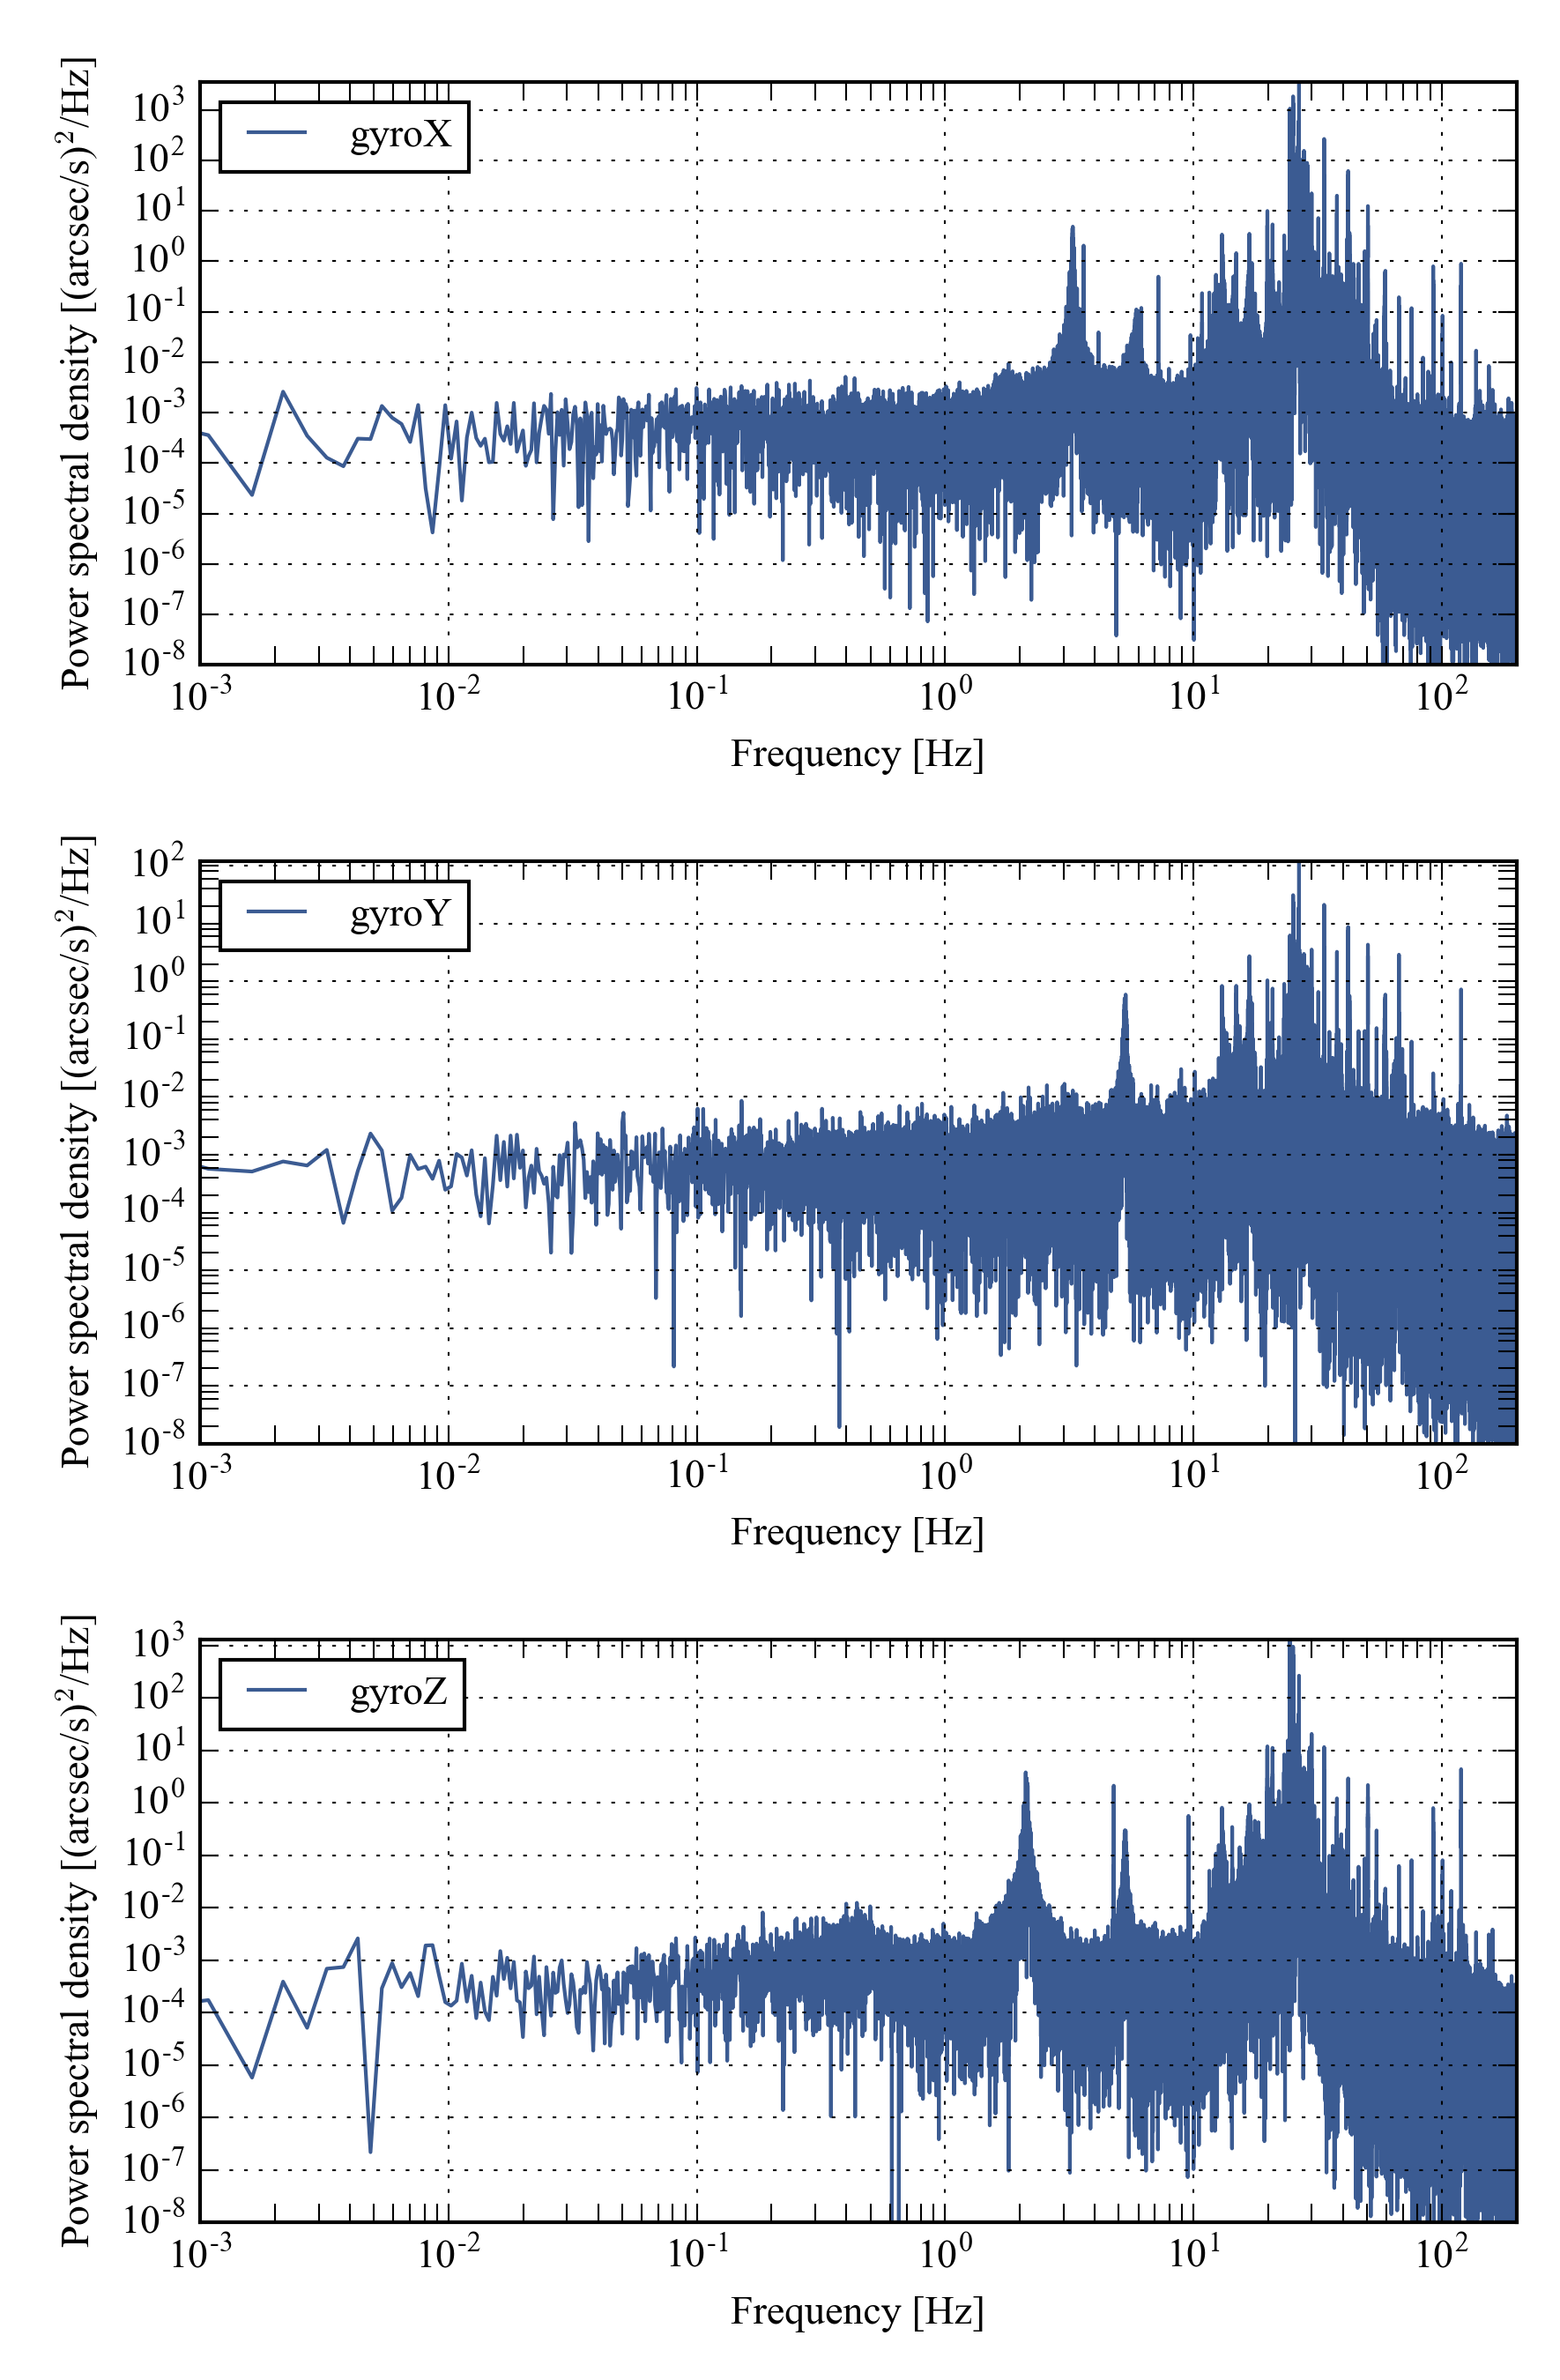
\includegraphics[width=\textwidth]{Figures/multiPSD400.png}
\label{fig:multiPSD400}
\vspace{-0.5cm}
\caption[Gyro PSD with payload on the ground]{Gyro PSD with payload on the ground}
\end{center}
\end{figure}

\begin{figure}[!h]
\begin{center}
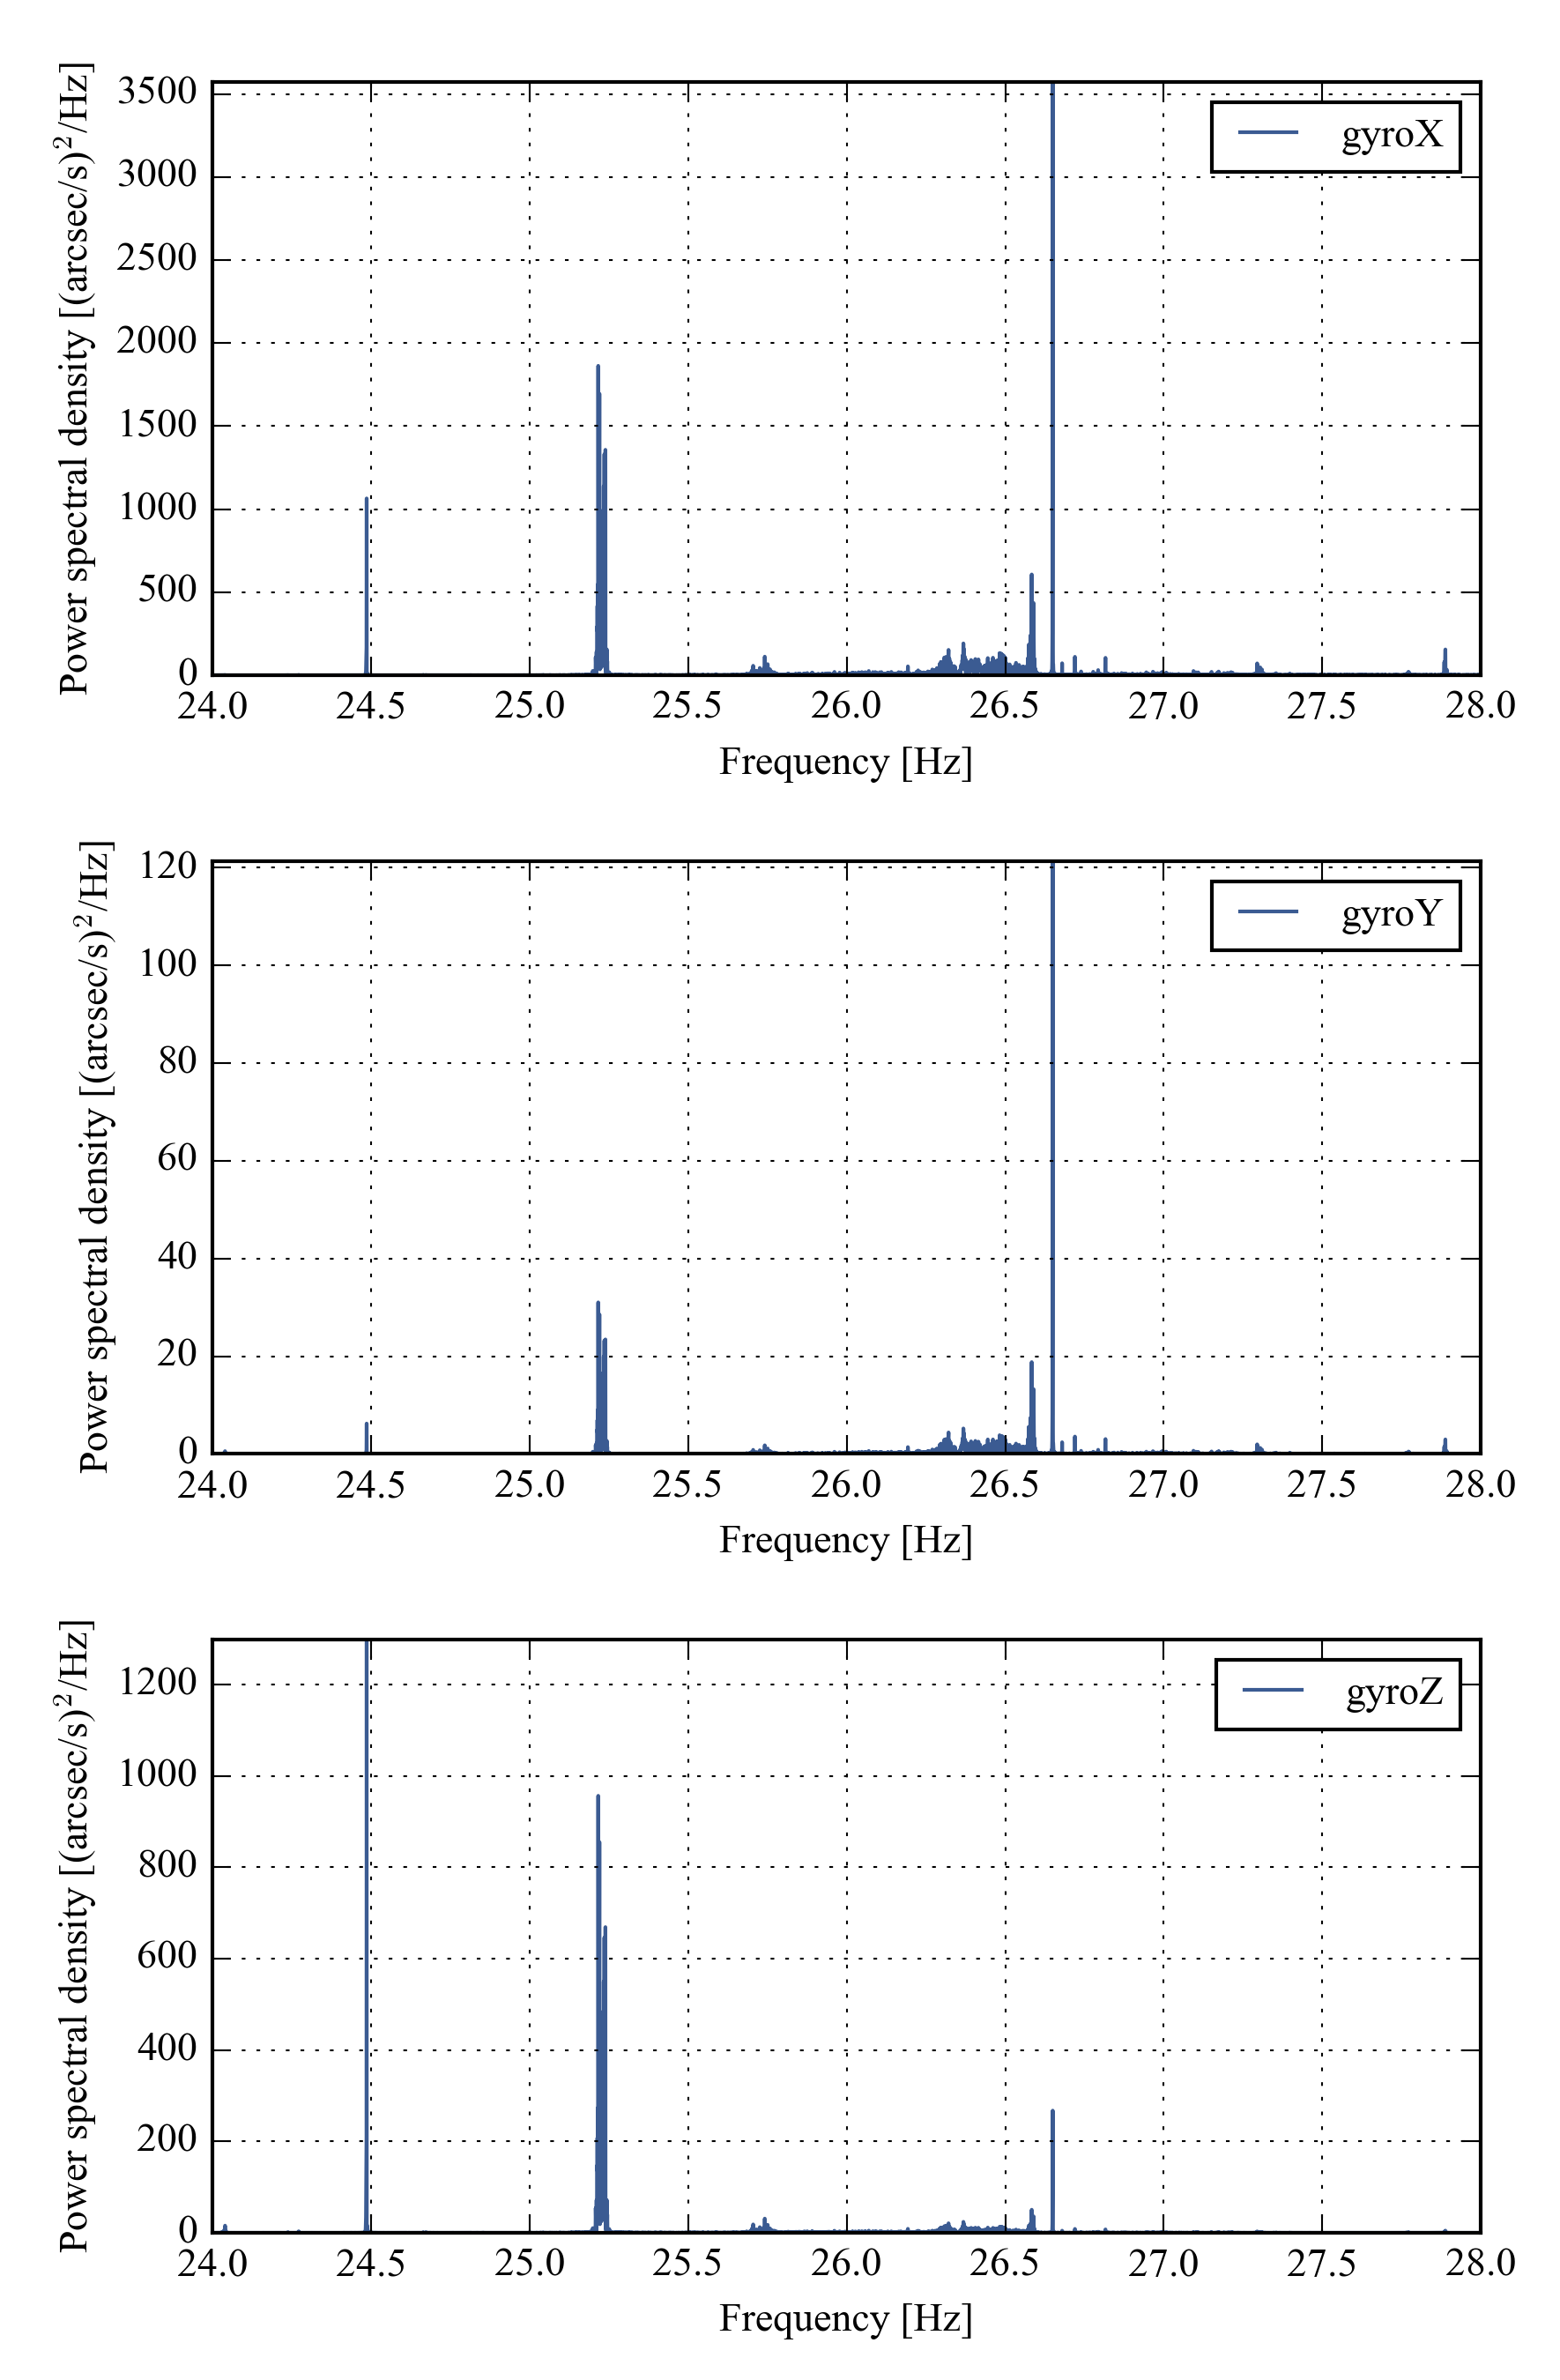
\includegraphics{Figures/multiPSD_no_loglog_zoom_400.png}
\label{fig:multiPSD400_no_loglog_zoom_400}
\vspace{-0.5cm}
\caption[Gyro PSD with payload on the ground - Main peaks]{Gyro PSD with payload on the ground - main peaks.}
\end{center}
\end{figure}



\subsubsection{Orthogonalization of gyroscope mount}
\label{ap:gyroOrth}
\subsubsection{Alignment of gyroscope mount to star camera mounts}

BETTII will have two flight star cameras for redundancy. It is important to understand the transformation between the gyroscope reference frame and the two star camera reference frames to minimize the propagation errors within the Kalman filter. 

A first transformation matrix can be estimated roughly by assuming that the star camera is in the ($\vectors{x}_\gyro$,$\vectors{z}_\gyro$) plane. The elevation of the star camera, nominally around \SI{45}{\degree}, can be estimated if $\vectors{z}$ is assumed to be aligned with the gravity vector while the payload is sitting on the ground, which is a good approximation. By taking some star camera measurements, solving the fields, and converting these fields to a local azimuth and elevation (using the time at which the frames were taken and the geographical location), the elevation can be estimated, which corresponds to the angle of the line of sight vector of the star camera with respect to the horizontal plane. This gives us a first estimate of our star camera-to-gyroscope reference frame rotation, but is not very precise given our assumptions. This rotation is critical during the update phase of the Kalman filter when combining the star camera measurement with the propagated estimate.

But if this matrix is slightly off, the Kalman filter will attribute the difference between estimated position and measured position as an additive bias error in the gyroscope velocity measurement, which should converge to a steady-state value after a few tens of star camera measurements, depending on the Kalman filter gains. The filter then uses this additive bias to reconstruct an estimated velocity at each time step. Admittedly, this value of the bias also contains the value of the real gyroscope bias - but we anticipate  this bias value to be very small compared to the potential effects of misalignments.

Our procedure involves calculating the quaternion representing the rotation from the steady-state estimated angular velocity vector, and the measured, orthogonalized angular velocity vector. While sitting on the ground, this corresponds to measuring the Earth's angular velocity. This uses the mathematical technique that we derived in Appendix~\ref{ap:rotBetweenTwoVec}. Each star camera measurement shall be further rotated by this quaternion to ensure that it is properly expressed in the gyroscope reference frame. 

Below, we summarize the steps to properly align the gyroscopes to the star camera:
\begin{enumerate}
 \item Orthogonalize the gyroscope mount according to Appendix~\ref{ap:gyroOrth}, and find $M_\textrm{orth}$. This now gives a velocity vector in an orthogonal gyro reference frame, $\gyroVec_\gyro$ = $M_\textrm{orth}\gyroVec_\gyro^\textrm{meas}$. 
 \item While the truss is sitting horizontal on the ground, calculate the elevation of the star camera by converting solutions to the local East-North-Up reference frame, using the sidereal time and the geographical latitude. This gives a matrix $M_\textrm{coarse}$  or a quaternion $\quat{q}_\textrm{coarse}$ representing the transformation from the star camera reference frame to the gyroscope reference frame.
\item Still while sitting on the ground, use $M_\textrm{coarse}$ or $\quat{q}_\textrm{coarse}$ in the flight Kalman filter to estimate the gyro bias vector. Record the steady-state value of the estimated velocity vector.
 \item Calculate the transformation between the estimated and measured angular velocity vector, this is a matrix $M_\textrm{fine}$ or a quaternion $\quat{q}_\textrm{fine}$.
 \item For each star camera reference frame solution, rotate the solution $\quat{q}_\textrm{fine}\quat{q}_\textrm{coarse}$.
 \item Use this new matrix in the flight Kalman filter to make sure the estimated biases are close to zero. 
 \end{enumerate} 
\subsection{Star camera}

\subsubsection{Tuning tests}

\renewcommand{\arraystretch}{1.5}
\setlist[itemize,1]{nolistsep,leftmargin=*,labelsep=-\mylen}
\def\labelitemi{--}
\begin{table}[!h]
\scriptsize
\caption[Star camera tests]{Star camera exposure time tests.}
\label{tab:starCameraTests}
\vspace{-0.5cm}
\begin{longtable}{l|P{1.5cm}P{1cm}P{1.5cm}P{1.5cm}P{1.5cm}P{1.5cm}P{1.5cm}P{1.5cm}}													
\toprule																							
{} 	&	  Exposure time (ms)	&	  Number of images in run 	&	  Fitted exposure time (ms)			&	  Number of matching stars 			&	  Fit ra \& dec error (arcsec) 			&	Fit roll error (arcsec)			&	  Processing time (s)			&	  Solution success rate (\%)	\\
\midrule																											
Exp1 	&	250	&	118	&	260	$\pm$	92	&	9.12	$\pm$	1.67	&	1.46	$\pm$	0.43	&	114	$\pm$	40	&	1.48	$\pm$	0.77	&	98	\\
Exp2 	&	125	&	36	&	113	$\pm$	13	&	9.75	$\pm$	1.95	&	1.46	$\pm$	0.39	&	118	$\pm$	32	&	1.05	$\pm$	0.26	&	100	\\
Exp3 	&	62	&	49	&	70	$\pm$	53	&	8.43	$\pm$	1.55	&	1.72	$\pm$	0.64	&	155	$\pm$	66	&	1.01	$\pm$	0.21	&	96	\\
Exp4 	&	62	&	132	&	66	$\pm$	23	&	7.32	$\pm$	1.34	&	1.75	$\pm$	0.65	&	151	$\pm$	55	&	1.22	$\pm$	0.59	&	76	\\
Exp5 	&	31	&	35	&	44	$\pm$	53	&	6.54	$\pm$	0.84	&	2.33	$\pm$	0.79	&	180	$\pm$	65	&	1.19	$\pm$	0.48	&	37	\\
\bottomrule
\end{longtable}																							
\end{table}																							

\begin{landscape}
\begin{figure}[!ht]
	\centering
	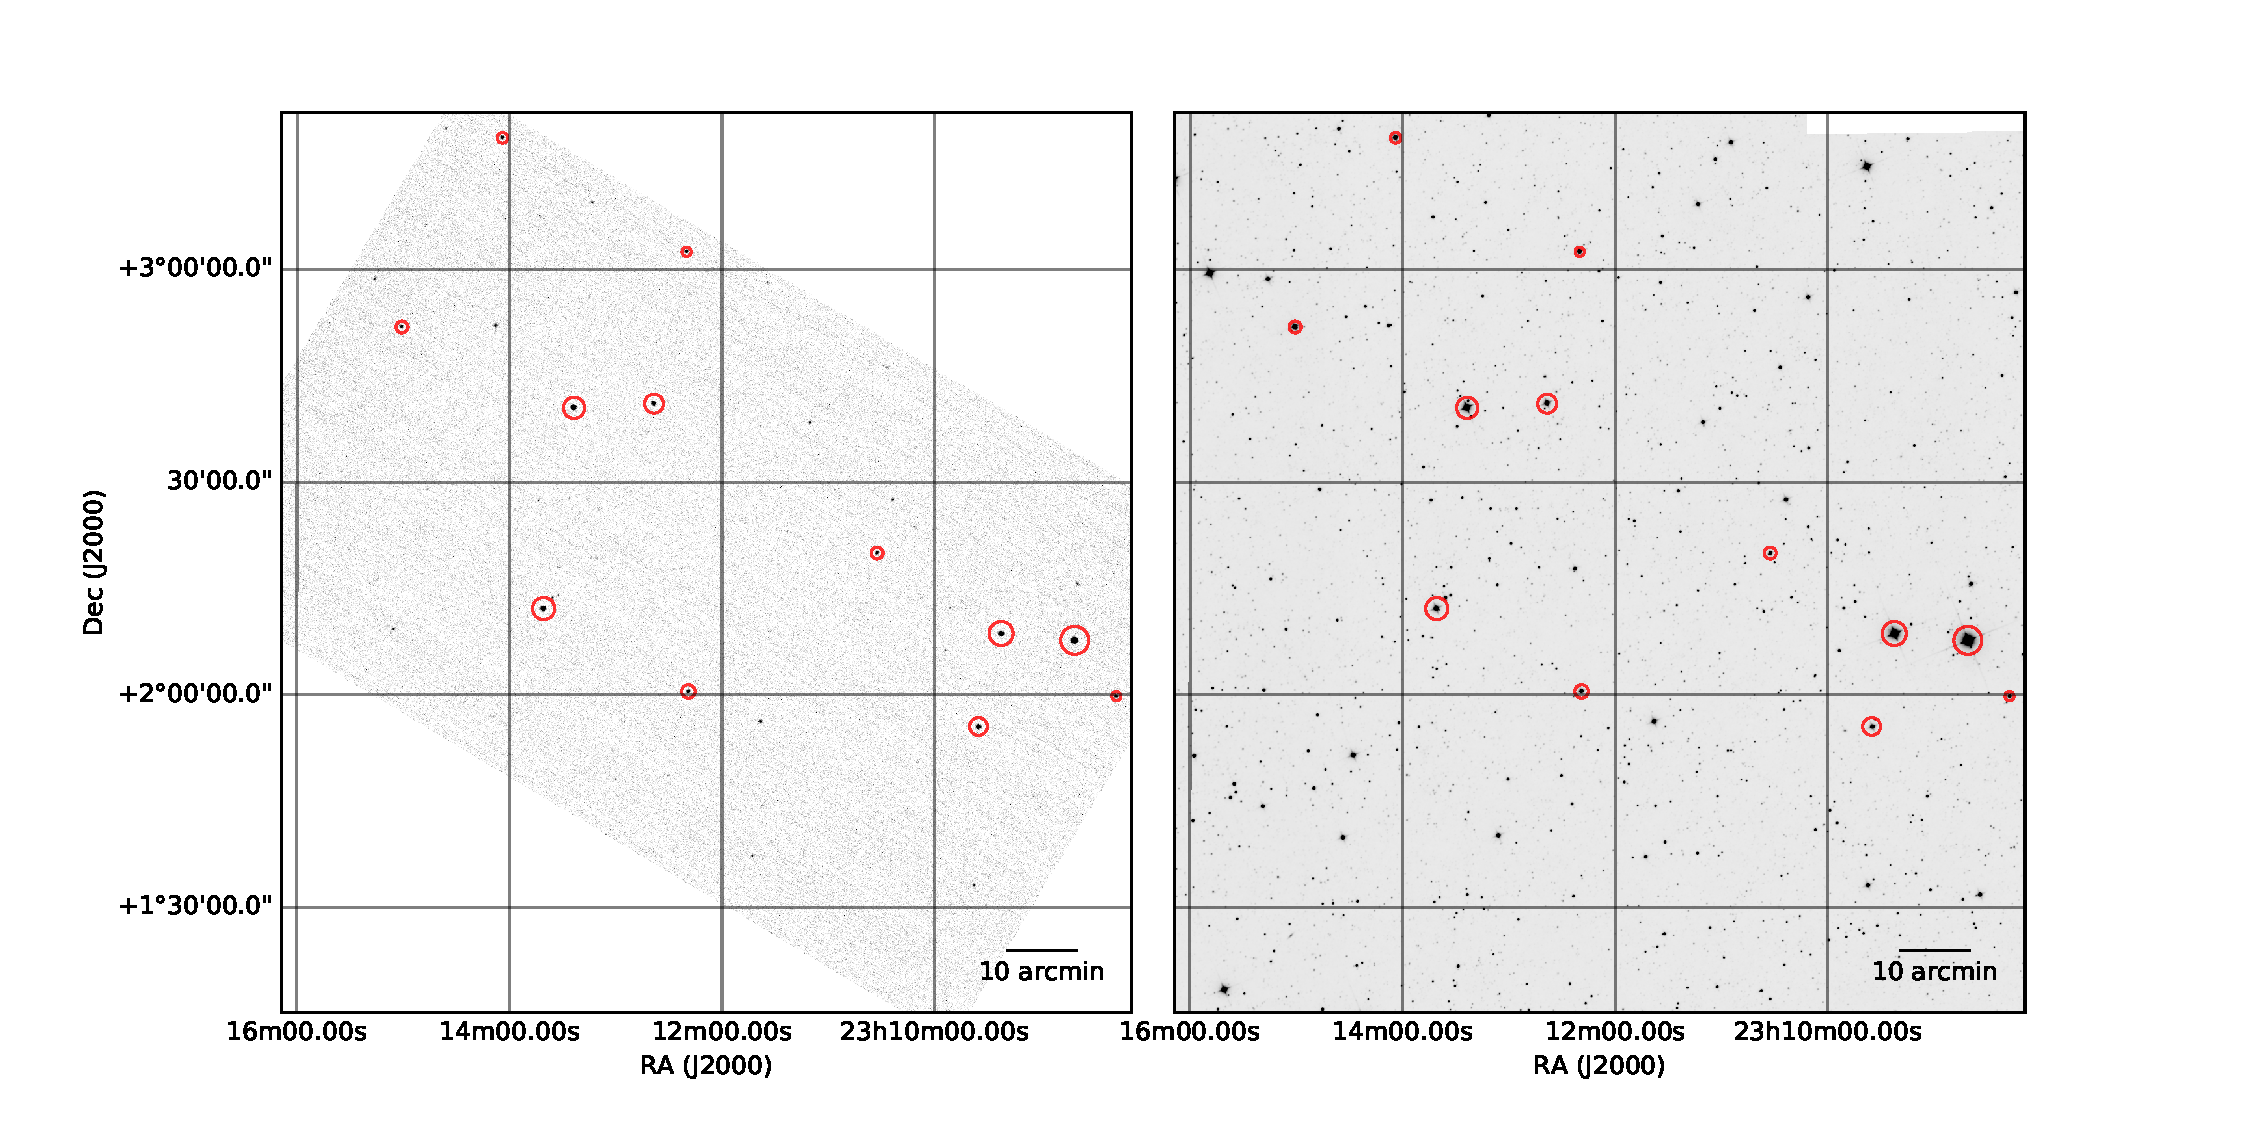
\includegraphics[width=1.5\textwidth]{Figures/starcam_images.pdf}
	\caption[Star camera example WISE]{\textit{Left}: Example of a background-subtracted star camera image with identified $>5\sigma$ sources circled in red. The orientation of the image on the celestial sphere is the one provided by BETTII's embedded star camera solver. This image corresponds to a field in the Scorpius constellation. \textit{Right}: WISE \SI{3.4}{\um} mosaic from the online archive, centered on the same location. This image is composed of 9 individual WISE images that we patched into a mosaic using the \textit{Montage}[CITE] software package.}
	\label{fig:starcamexample}
    \end{figure}
\end{landscape}
\begin{landscape}
\begin{figure}[!ht]
	\centering
	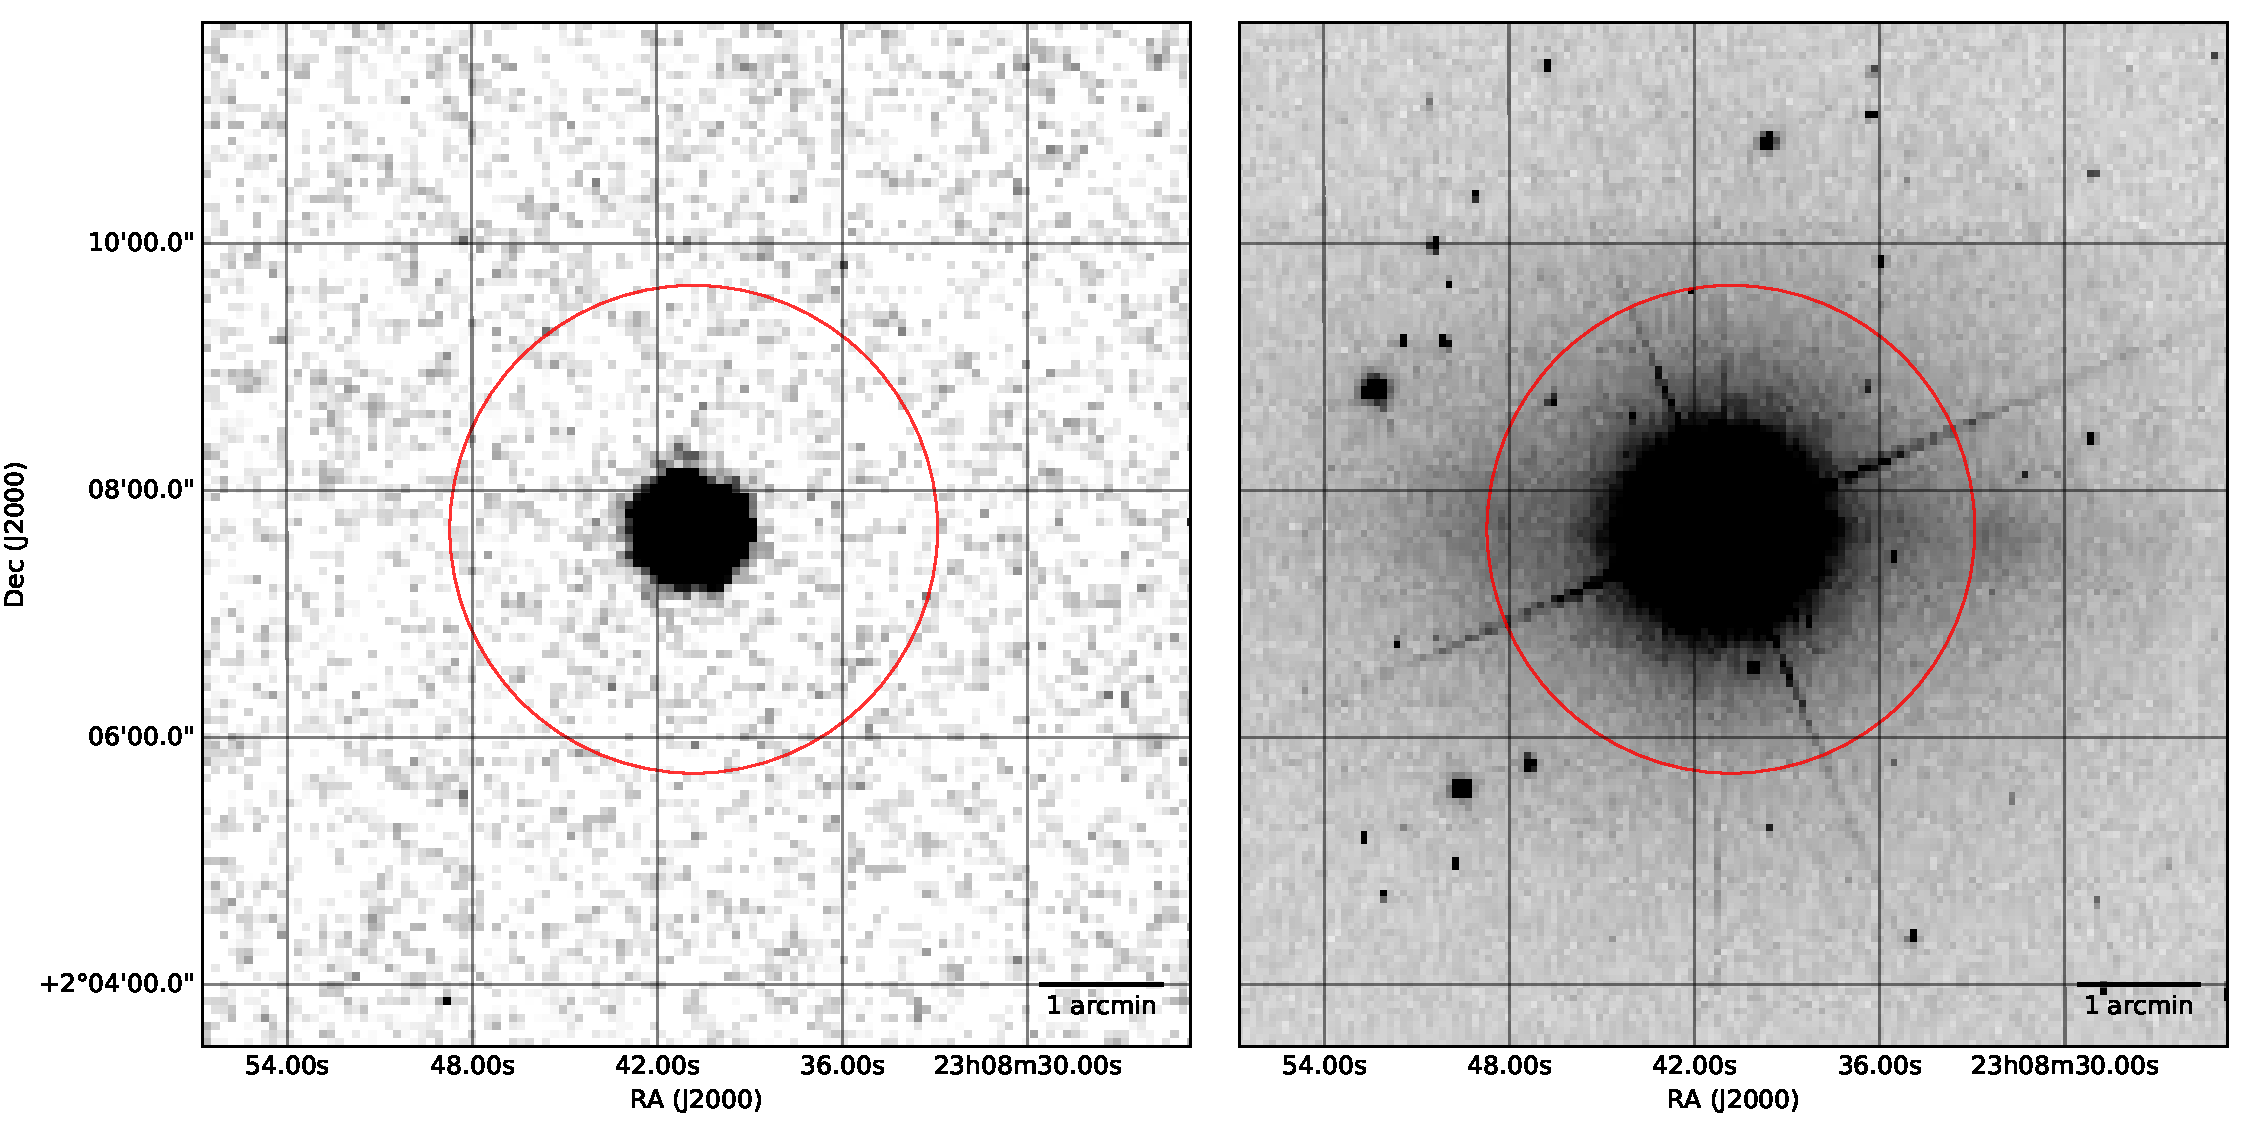
\includegraphics[width=1.5\textwidth]{Figures/starcam_SDSSr_zoom.pdf}
	\caption[Star camera individual star]{\textit{Left}: Snapshot of a bright star seen within the background-subtracted star camera frame. \textit{Right}: Snapshot taken at the same location from the WISE \SI{3.4}{\um} archive.}
	\label{fig:starcamzoom}
    \end{figure}
\end{landscape}

Discuss about tuning, catalog, filters, etc

Table with the star camera parameters

Show mean deviation of star camera image with optimized parameters;
show time, statistics, etc.

\subsubsection{Final parameters}

\section{Test setups and limitations}
\subsection{Talk about the way we test in the high bay, etc}
\subsection{List of test setups: gyro only, gyro+star camera, gyro+star camera+tip/tilts with CCD cameras, gyro+star camera with H1RG;}
\subsection{Explain the communication/data recording approach}

\subsection{Autofocus algorithm and performance}

\section{Estimator implementation}
\subsection{Gyro attitude estimator}
\documentclass{standalone}
\usepackage{tikz}
\usetikzlibrary{shapes,arrows}

\begin{document}
\tikzstyle{block} = [draw, fill=black!20, rectangle, 
    minimum height=3em, minimum width=6em,align=center]
\tikzstyle{input} = [node distance=1cm]
\tikzstyle{output} = [node distance=1cm]
\newpage
\begin{tikzpicture}[auto, >=latex',scale=0.8, every node/.style={transform shape}]
\linespread{1}


% Inputs
\node [input,name=measuredVelocity,shift={(2cm,0cm)}] {$\gyroVec^{\textrm{meas}}_k$};
\node [input,above of=measuredVelocity,name=bias] {$\EstBias_{k|k-N}$};
\node [input,above of=bias,name=attitude,node distance=1cm] {$\EstAttitude_{k-1|k-N}$};
\node [input,above of=measuredVelocity,name=covariance,node distance=3cm] {$\noiseCovMat_k$};
\node [input,below of=measuredVelocity,name=propagation matrices,node distance=4cm] {$\A_{k-1},\B_{k-1},\C_{k-1}$};

% line break
\node [input,name=line break left,above of=covariance,node distance=2cm] {};
\node [input,name=line break left2,below of=line break left,node distance=0.5cm,right] {\large \textbf{Kalman Filter: Prediction}};
\node [input,name=line break right,right of=line break left,node distance=15cm] {\large { }};
\draw[dashed] ([xshift=-1cm]line break left.north west) -- (line break right.north east);


% blocks
\node [block, right of=measuredVelocity,node distance=3cm] (estimate velocity) {Estimate \\ Velocity};
\node [block, right of=estimate velocity,node distance=4cm] (predict attitude) {Predict \\ Attitude};
\node [block, below of=predict attitude,node distance=2cm] (state transition) {State \\ transition};
\node [block, right of=state transition,node distance=4cm] (estimate covariance) {Estimate \\ covariance};
\node [block, below of=estimate covariance,node distance=2cm] (update propagation matrices) {Propagate \\ matrices};

% outputs
\node [output,right of=predict attitude,node distance=3cm,name=estattitude]{};
\node [output,right of=estimate covariance,node distance=3cm,name=estcovariance]{};
\node [output,right of=update propagation matrices,node distance=3cm,name=propmat]{};

% arrows
\draw[->] (bias.east) -| (estimate velocity.north);
\draw[->] (measuredVelocity.east) -- (estimate velocity.west);

\node[name=mid,right of=estimate velocity,node distance=2cm,draw,fill,minimum size=3pt,circle]{};
\node[above] at (mid){$\EstGyroVec_{k|k-N}$};
\draw[->] (estimate velocity.east) -- (mid) -- (predict attitude.west);
\draw[->] (attitude.east) -| (predict attitude.north);
\draw[->] (mid) |- (state transition.west) ;
\node[name=mid,right of=state transition,node distance=2cm,draw,fill,minimum size=3pt,circle]{};
\node[above] at (mid){$\StateTransitionMat_k$};
\draw[->] (state transition.east) -- (mid) -- (estimate covariance.west) ;
\node[name=mid2,below of=mid,node distance=1cm,outer sep=0cm,inner sep=0cm]{};
\draw[-] (mid) --  (mid2.north) ;
\draw[->] (mid2.north) -|  (update propagation matrices.north) ;

\node[name=mid,right of=estimate covariance,node distance=3cm]{};
\node[above] at (mid){$\stateCovMat_{k|k-N}$};
\draw[->] (estimate covariance.east) -- (estcovariance) ;
\draw[->] (covariance.east) -| (estimate covariance.north) ;

\node[name=mid,right of=predict attitude,node distance=3cm]{};
\node[above] at (mid){$\EstAttitude_{k|k-N}$};
\draw[->] (predict attitude.east) -- (mid);

\draw[->] (propagation matrices.east) -- (update propagation matrices.west);
\draw[->] (update propagation matrices.east) -- (propmat);
\node[name=mid,right of=update propagation matrices,node distance=3cm]{};
\node[above] at (mid){$\A_{k},\B_{k},\C_{k}$};


% Kalman Update
% line break
\node [input,name=line break left,below of=propagation matrices,node distance=1.5cm] {};
\node [input,name=line break left2,below of=line break left,node distance=0.5cm,right] {\large \textbf{Kalman Filter: Update}};
\node [input,name=line break right,right of=line break left,node distance=15cm] {\large { }};
\draw[dashed] ([xshift=-1cm]line break left.north west) -- (line break right.north east);

% Inputs
\node [input,name=measured attitude,below of=line break left,node distance=3cm] {$\Attitude^\textrm{meas}_{\starcam}$};
\node [input,name=final matrices,above of=measured attitude,node distance=1cm] {$\A_{k},\B_{k},\C_{k}$};
\node [input,name=covmat,below of=measured attitude,node distance=6cm] {$\stateCovMat_{k|k-N}$};
\node [input,name=meascovmat,below of=measured attitude,node distance=2cm] {$\measCovMat_{k}$};

% blocks
\node [block, right of=measured attitude,node distance=3cm] (propagate attitude) {Rotate \& \\ Propagate};
\node [block, below of=propagate attitude,node distance=2cm] (innovation) {Innovation};
\node [block, below of=innovation,node distance=2cm] (innovation covariance) {Innovation \\ covariance};
\node [block, below of=innovation covariance,node distance=2cm] (kalman gain) {Kalman \\ gain};
\node [block, right of=kalman gain,node distance=4cm] (calculate error) {Calculate \\ error};
\node [block, right of=calculate error,node distance=4cm] (update bias) {Update \\ bias};
\node [block, below of=update bias,node distance=2cm] (update attitude) {Update \\ attitude};
\node [block, above of=update bias,shift={(3cm,1cm)}] (update velocity) {Update \\ velocity};
\node [block, below of=update attitude,node distance=2cm] (update covariance) {Update \\ covariance};

% arrows
\draw[->] (measured attitude) -- (propagate attitude);
\draw[->] (final matrices) -| (propagate attitude);
\draw[->] (propagate attitude.south) -- (innovation.north);
\draw[->] (innovation covariance.south) -| (kalman gain.north);
\draw[->] (covmat.east) -- (kalman gain.west);
\draw[->] (covmat.north) |- (innovation covariance.west);
\draw[->] (meascovmat.east) -- (innovation.west);
\draw[->] (covmat.south) |- (update covariance.190);

% intermediary nodes
\node[name=mid,right of=kalman gain,node distance=2cm,draw,fill,minimum size=3pt,circle]{};
\node[above] at (mid){$\KalmanGain_{k}$};
\draw[->] (kalman gain.east) -- (mid) -- (calculate error.west);
\draw[->] (mid) |- (update covariance.165);

\node[name=mid,below of=propagate attitude,node distance=1cm]{};
\node[left] at (mid){$\Attitude^{\textrm{meas}}_{k}$};


\node[name=mid,below of=innovation,node distance=1cm,draw,fill,minimum size=3pt,circle]{};
\node[left] at (mid){$\zMeasurement_{k}$};
\draw[->] (mid) -| (calculate error.north);
\draw[->] (innovation.south) -- (mid) -- (innovation covariance.north);

\node[name=mid,below of=innovation covariance,node distance=1cm]{};
\node[left] at (mid){$\measErrCovMat_{k}$};


\node[name=mid,right of=calculate error,node distance=2cm,draw,fill,minimum size=3pt,circle]{};
\node[above] at (mid){$\ErrorState_{k|k}$};
\draw[->] (calculate error.east) -- (mid) -- (update bias.west);

\node [input,name=bias estimate,above of=mid,shift={(1cm,0cm)}] {$\EstBias_{k|k-N}$};
\draw[->] (bias estimate) -| (update bias.north);

\node [input,name=attitude estimate,below of=bias estimate,node distance=2cm] {$\EstAttitude_{k|k-N}$};
\draw[->] (attitude estimate) -| (update attitude.north);


\node [input,name=velocity estimate,above of=bias estimate,node distance=2cm] {$\EstGyroVec_{k|k-N}$};
\draw[->] (velocity estimate) -| (update velocity.north);
\draw[->] (mid) |- (update attitude.west);

\node [output,name=velocity,right of=update velocity,node distance=2cm]{}; \node [output,right of=update velocity,node distance=2cm,above] {$\EstGyroVec_{k|k}$};
\draw[->] (update velocity.east) -- (velocity);

% outputs
\node [output,name=mid,right of=update bias,node distance=3cm,draw,fill,minimum size=3pt,circle] {};
\draw[->] (update bias.east) -- (mid);
\draw[->] (mid) -- (update velocity.south);
\node [output,name=bias,right of=mid,node distance=2cm] {};
\node [output,right of=mid,node distance=2cm,above] {$\EstBias_{k|k}$};
\draw[->] (mid) -- (bias.west);
\node [output,name=attitude,right of=update attitude,node distance=2cm] {};
\node [output,right of=update attitude,node distance=2cm,above] {$\EstAttitude_{k|k}$};
\draw[->] (update attitude) -- (attitude);

\node [output,name=covariances,right of=update covariance,node distance=2cm] {};
\node [output,right of=update covariance,node distance=2cm,above] {$\stateCovMat_{k|k}$};
\draw[->] (update covariance) -- (covariances);

\end{tikzpicture}
\end{document}

\subsubsection{Testing the Kalman filter software with simulated data}
\subsubsection{Test results when sitting on the ground}
\subsection{Telescope attitude estimator}
Link to cross-elevation
\subsection{Phase estimator [is that Arnab’s realm?]}

\section{Operating modes}
\subsection{Track mode}
Gain tuning
Show wheel angle for long time
\subsection{Slew mode}
\subsection{Acquire mode [this one is contingent on the telescopes working, and is not perfectly representative when only using one single side of the payload]}

\section{Pointing tests and performance results}
\subsection{Gondola pointing stability}
\subsubsection{In the high bay}

\begin{figure}[!ht]
\begin{center}
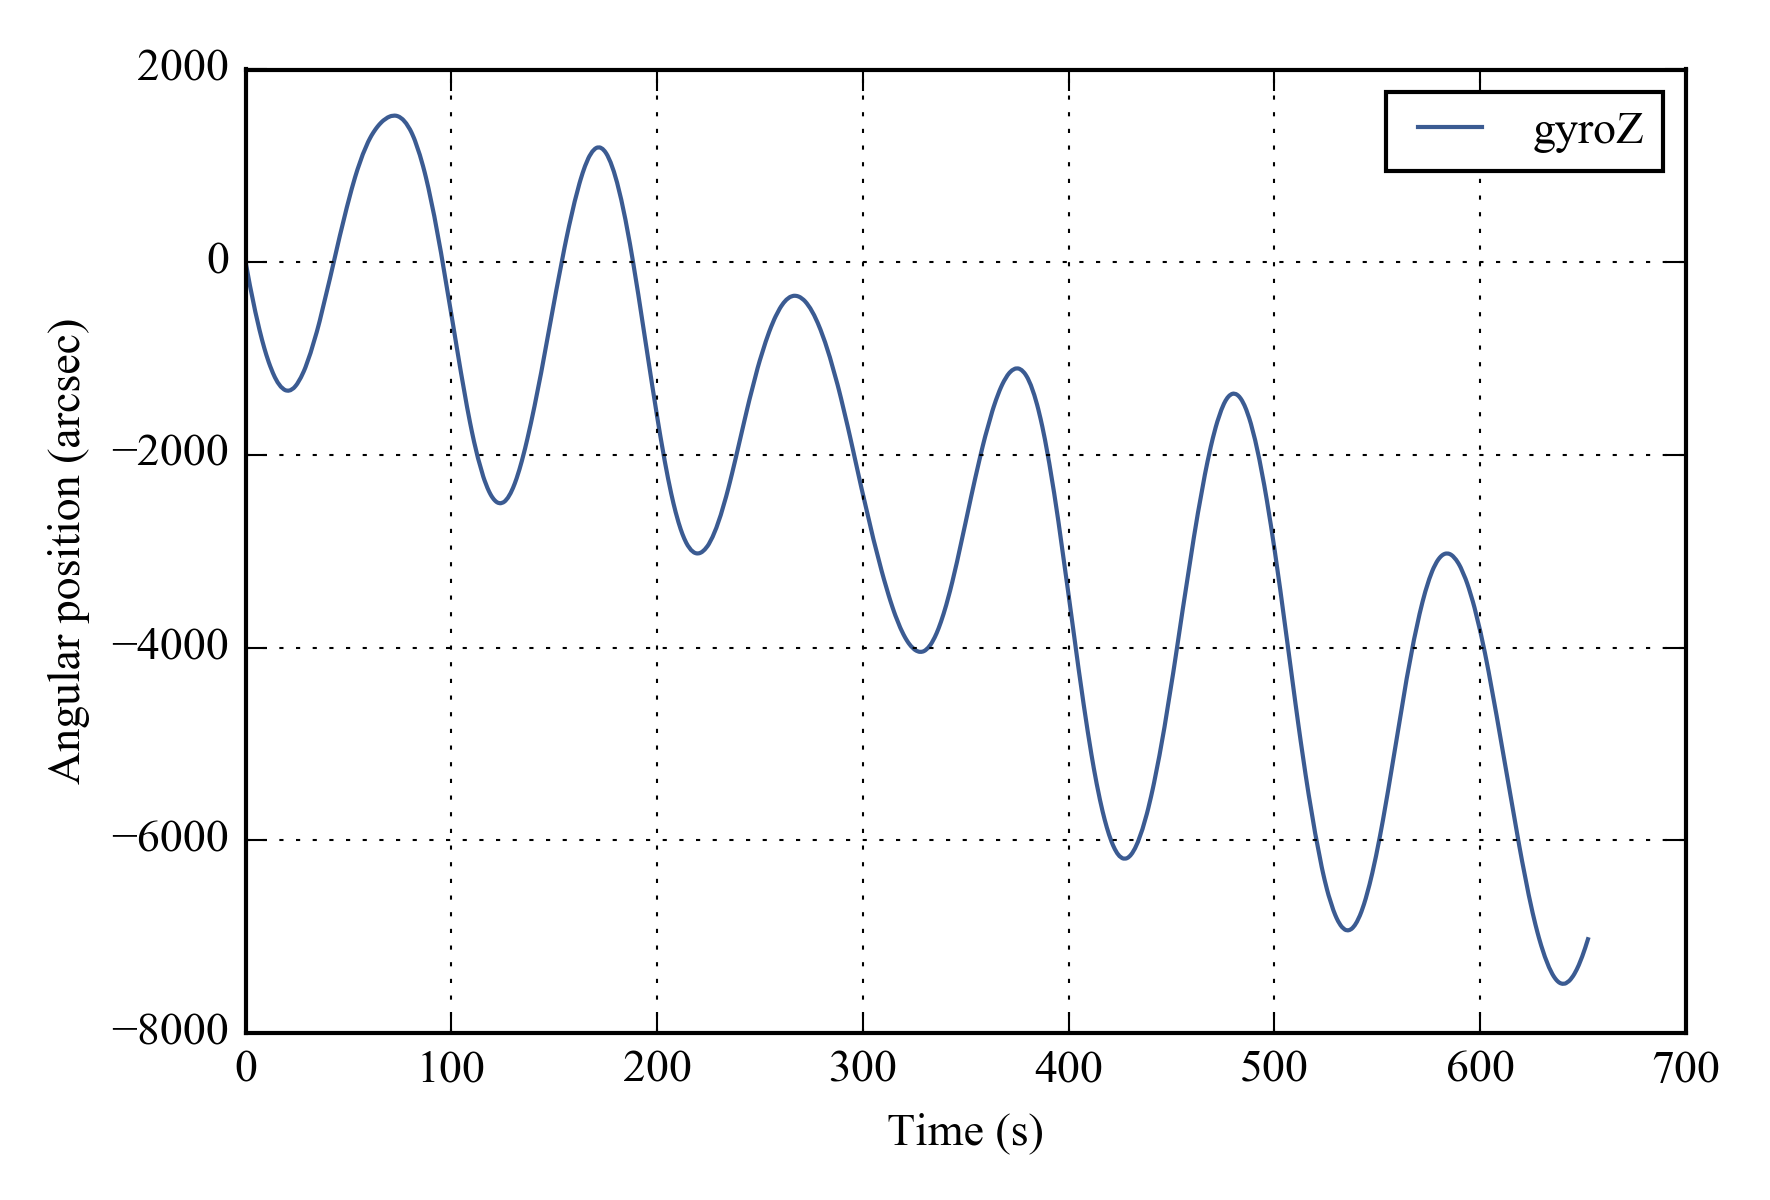
\includegraphics{Figures/integral_lifted_gyroZ.png}
\label{fig:intgralgyroZ400}
\vspace{-0.5cm}
\caption[Integrated gyro time series while hanging]{Integrated gyro time series while hanging and no motor on.}
\end{center}
\end{figure}
\begin{figure}[!h]
\begin{center}
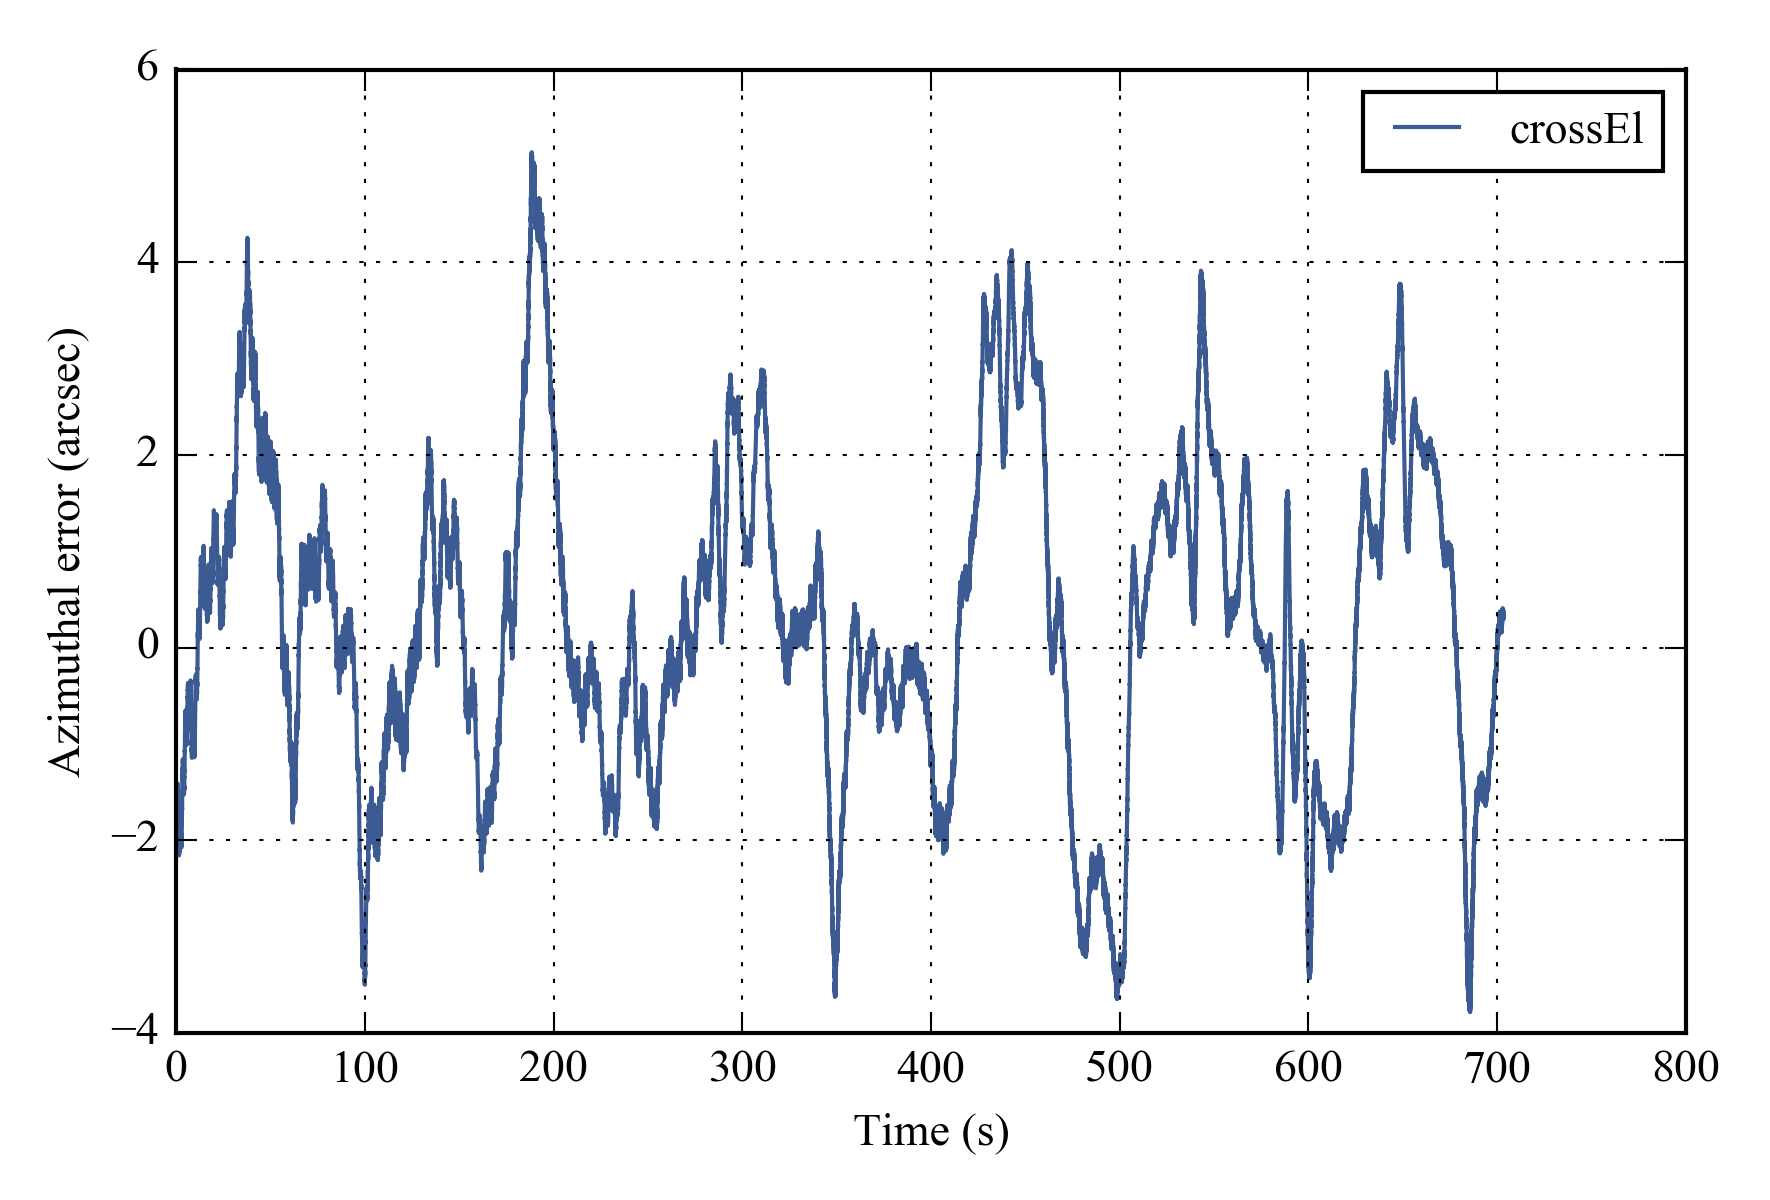
\includegraphics[width=\textwidth]{Figures/simplePlot_crossEl.png}
\label{fig:crossEl400}
\vspace{-0.5cm}
\caption[Cross-elevation with control loop on]{Cross-elevation with control loop on (gyroscopes only).}
\end{center}
\end{figure}




\begin{figure}[!h]
\begin{center}
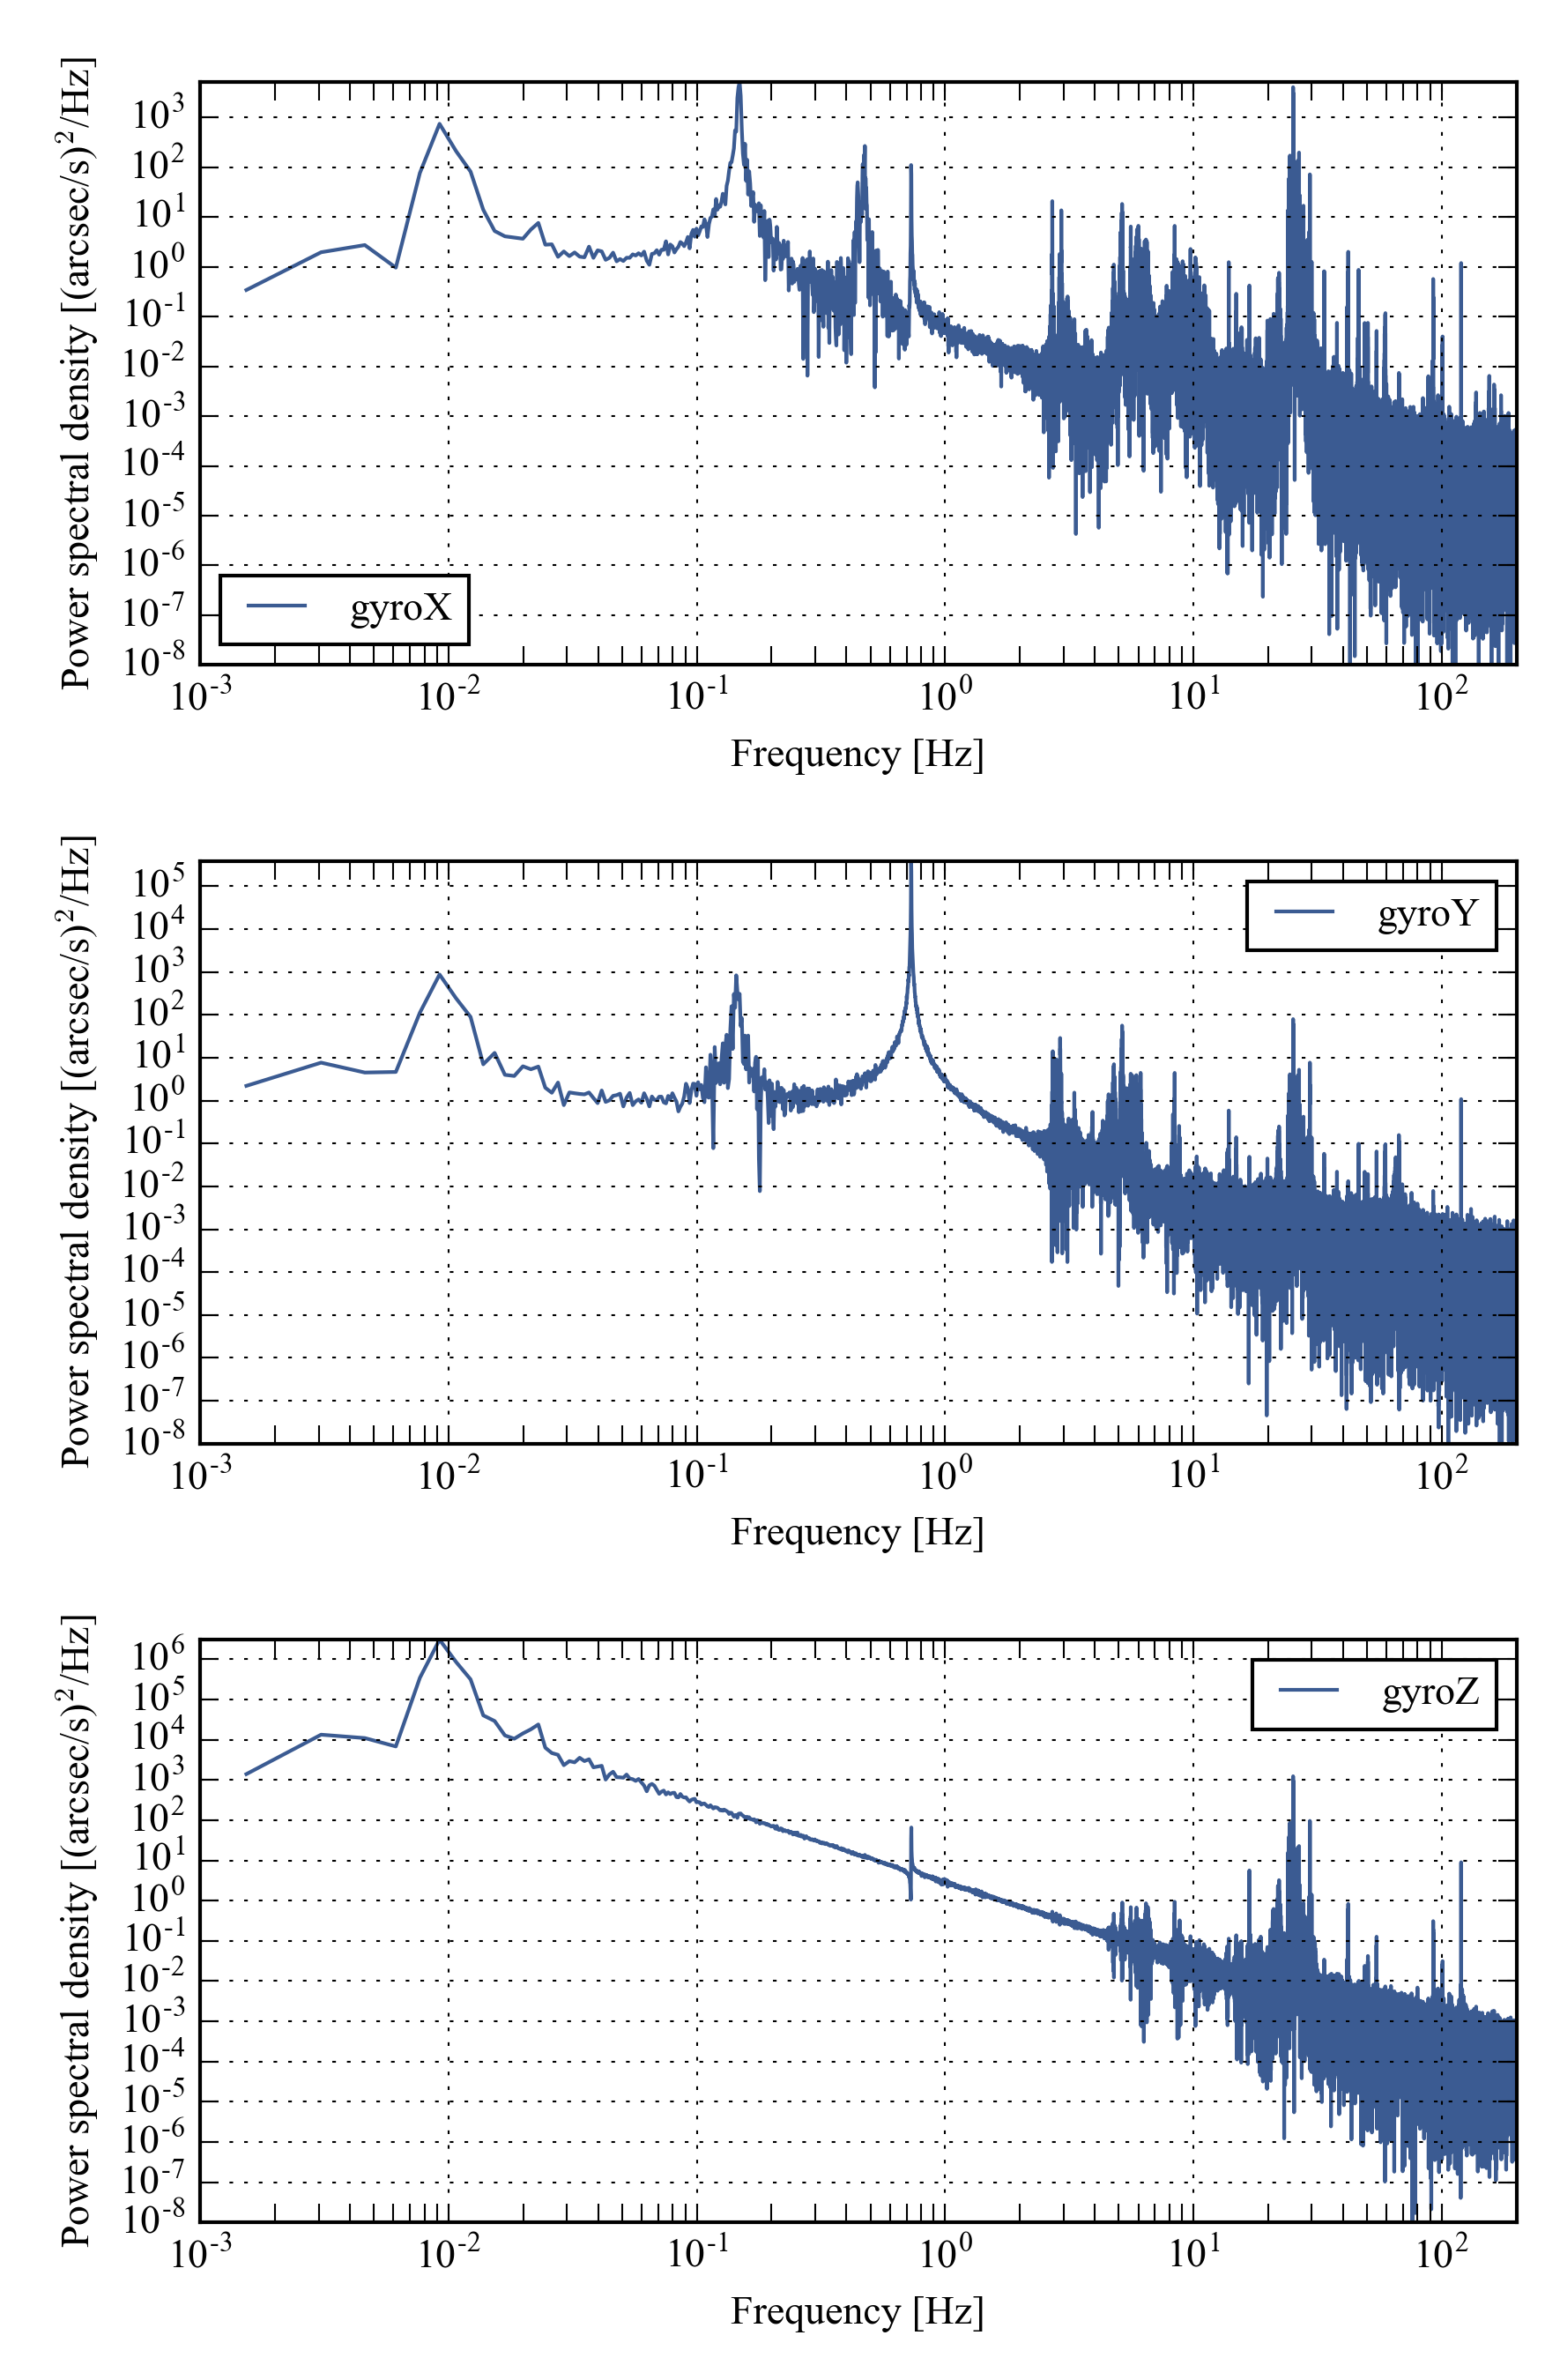
\includegraphics{Figures/lifted_400.png}
\label{fig:multiPSD400_lifted}
\vspace{-0.5cm}
\caption[Gyro PSD with payload lifted]{Gyro PSD with payload lifted.}
\end{center}
\end{figure}


\begin{figure}[!h]
\begin{center}
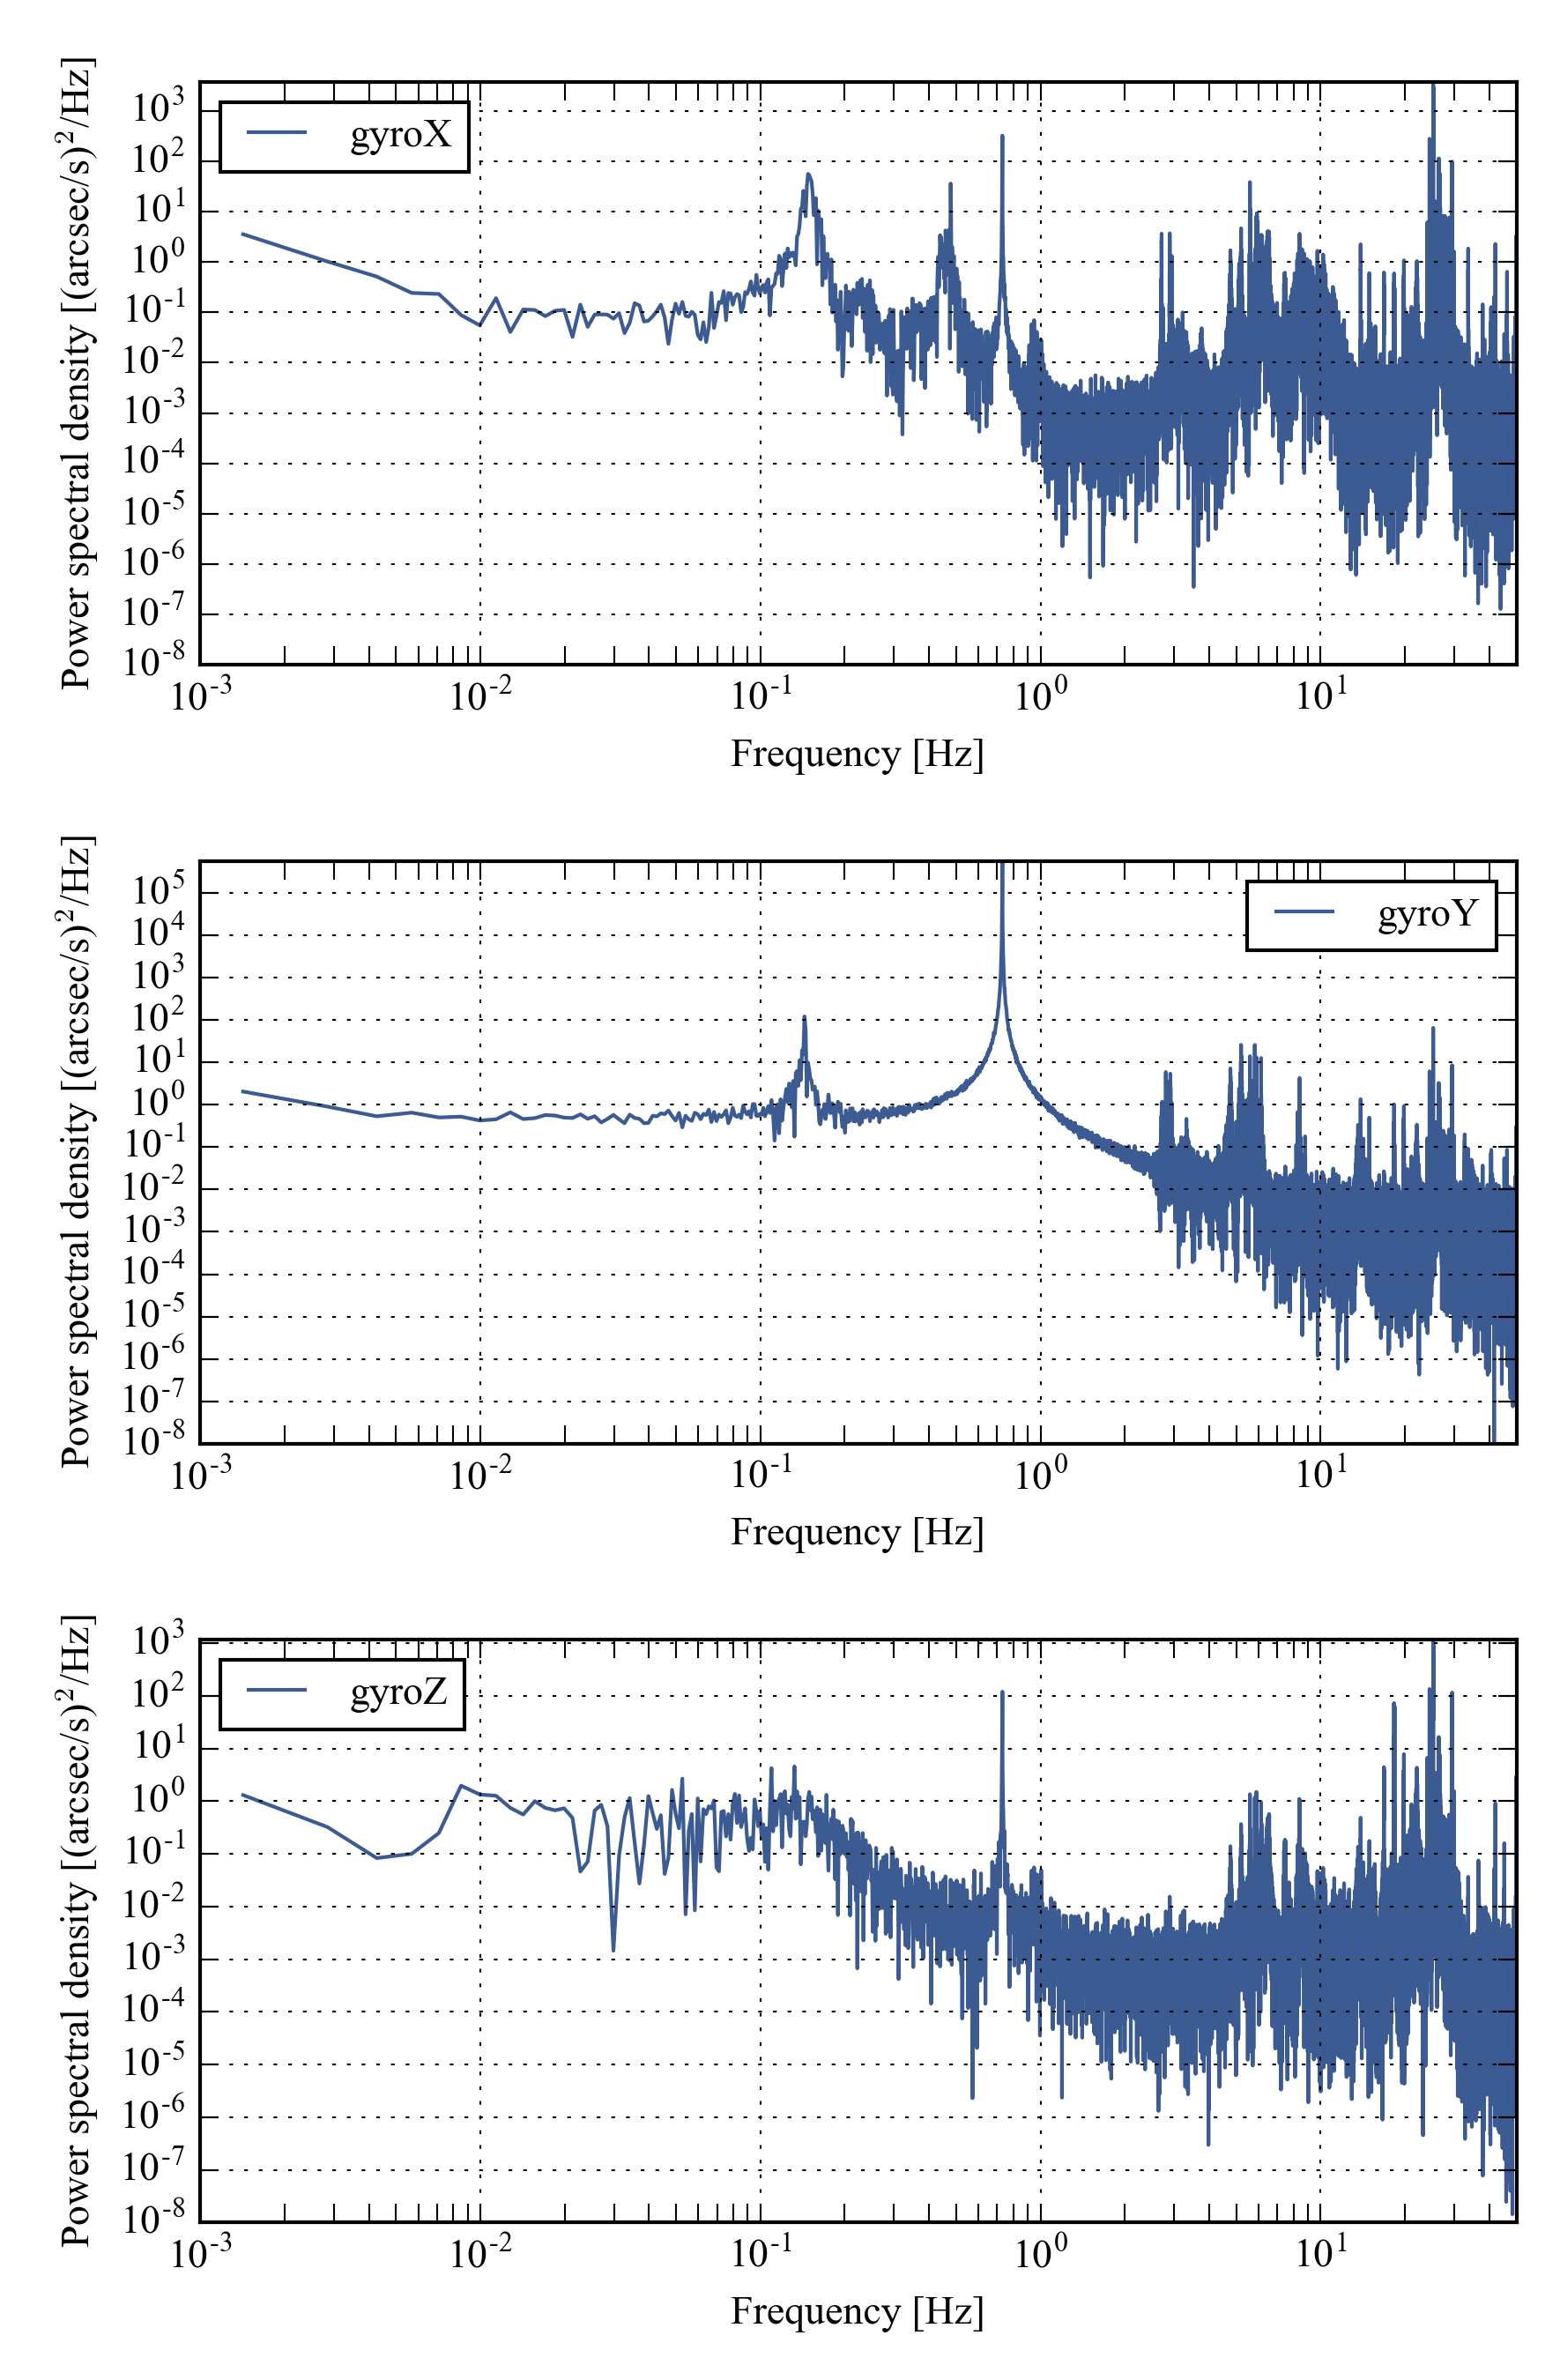
\includegraphics{Figures/multiPSD100.png}
\label{fig:multiPSD100_controlled}
\vspace{-0.5cm}
\caption[Gyro PSD with payload lifted, under azimuth control]{Gyro PSD with payload under azimuth control.}
\end{center}
\end{figure}


 show azimuth stability data
show telescope rolling rms
\subsubsection{With the door open}
\subsection{Kalman filter performance}
Show data with the door open with the star camera acquiring frames
\subsection{gyro+star camera+tip/tilts with CCD cameras}
\subsection{gyro+star camera with H1RG;}

\section{	Using the test results to estimate the flight performance (have to think more about that section)}
\subsection{Perturbation rejection estimates}
\subsection{Pointing knowledge predictions}
\subsection{Pointing control predictions}
 
%\chapter{Star Formation in Clustered environments with SOFIA FORCAST}

\label{chap:SOFIA}

\section{Introduction}
Most stars in the Galaxy form in cluster environments of sizes 2-4 pc, often containing more than 100 young stellar objects (YSOs), with typical separations of $<$0.05~pc between stars near their centers \citep{Porras:2003kxa, Allen:2007wqa, Gutermuth:2009gca}.
Previous studies have been effective in elucidating the young stellar content and distribution in clouds on large scales (parsec down to 0.05~pc) \citep{Evans-ARAA2012}, but young cluster cores, born in dense portions of molecular clouds, are more difficult to observe. They are obscured at optical through near-IR wavelengths. At mid-IR through far-IR wavelengths, the material surrounding YSOs and involved in the stellar birth process emits due to heating by the young stars, but the resolution to date has not been sufficient to isolate individual stars in the cores of most nearby young clusters.


%\begin{enumerate}
%\item Description of the sample and the goals
%\item Description of the data we used: 2MASS, Spitzer, Herschel; SOFIA
%\item Instrument characterization
%\item Explain the data reduction process; include comparison with Megeath for Spitzer photometry; justify aperture correction with "total cluster" measurements
%\item Data products: maps, SEDs; spectral index distribution, Lbol, Tbol
%\item SED fitting method \& grid description (e.g. color-color diagram?)
%\item Focus on IRAS20050 and NGC2071 + Ophiuchus? SED fitting; our method, our results; analysis of the results similar to furlan?
%\item 
%\end{enumerate}
%SOFIA has a \SI{2.7}{\meter} primary mirror which is a significant size improvement over \Spitzer. The instrument we have used, FORCAST, provides unprecedented high angular resolution of \ang{;;2}-\ang{;;3.5} in multiple continuum bands from \SI{5.5}{\micro\meter} to \SI{37.1}{\micro\meter}, which allows us to probe a relatively unexplored region of phase space. We discuss our SOFIA project in Chapter~[].


\section{Sample description and scientific goals}

\Spitzer has tremendously helped our understanding of star formation, by providing sensitive observations in continuum bands from \SI{3.6}{\um} to \SI{160}{\micro\meter}. In particular, the MIPS \SI{24}{\micro\meter} channel provided a robust way to determine the spectral index of YSOs, hence leading to dramatic improvement of understanding of the YSO population in clusters \citep[e.g.,][]{Gutermuth:2009gca,Gutermuth:2011he}.

However, the most dense regions of clusters still present a challenge for the MIPS instrument, as the YSOs are too bring and/or in too close proximity, which leads to saturation and confusion, as exhibited in Fig.~\ref{fig:NGC2071saturated}. 

\begin{figure}[!h]
\begin{center}
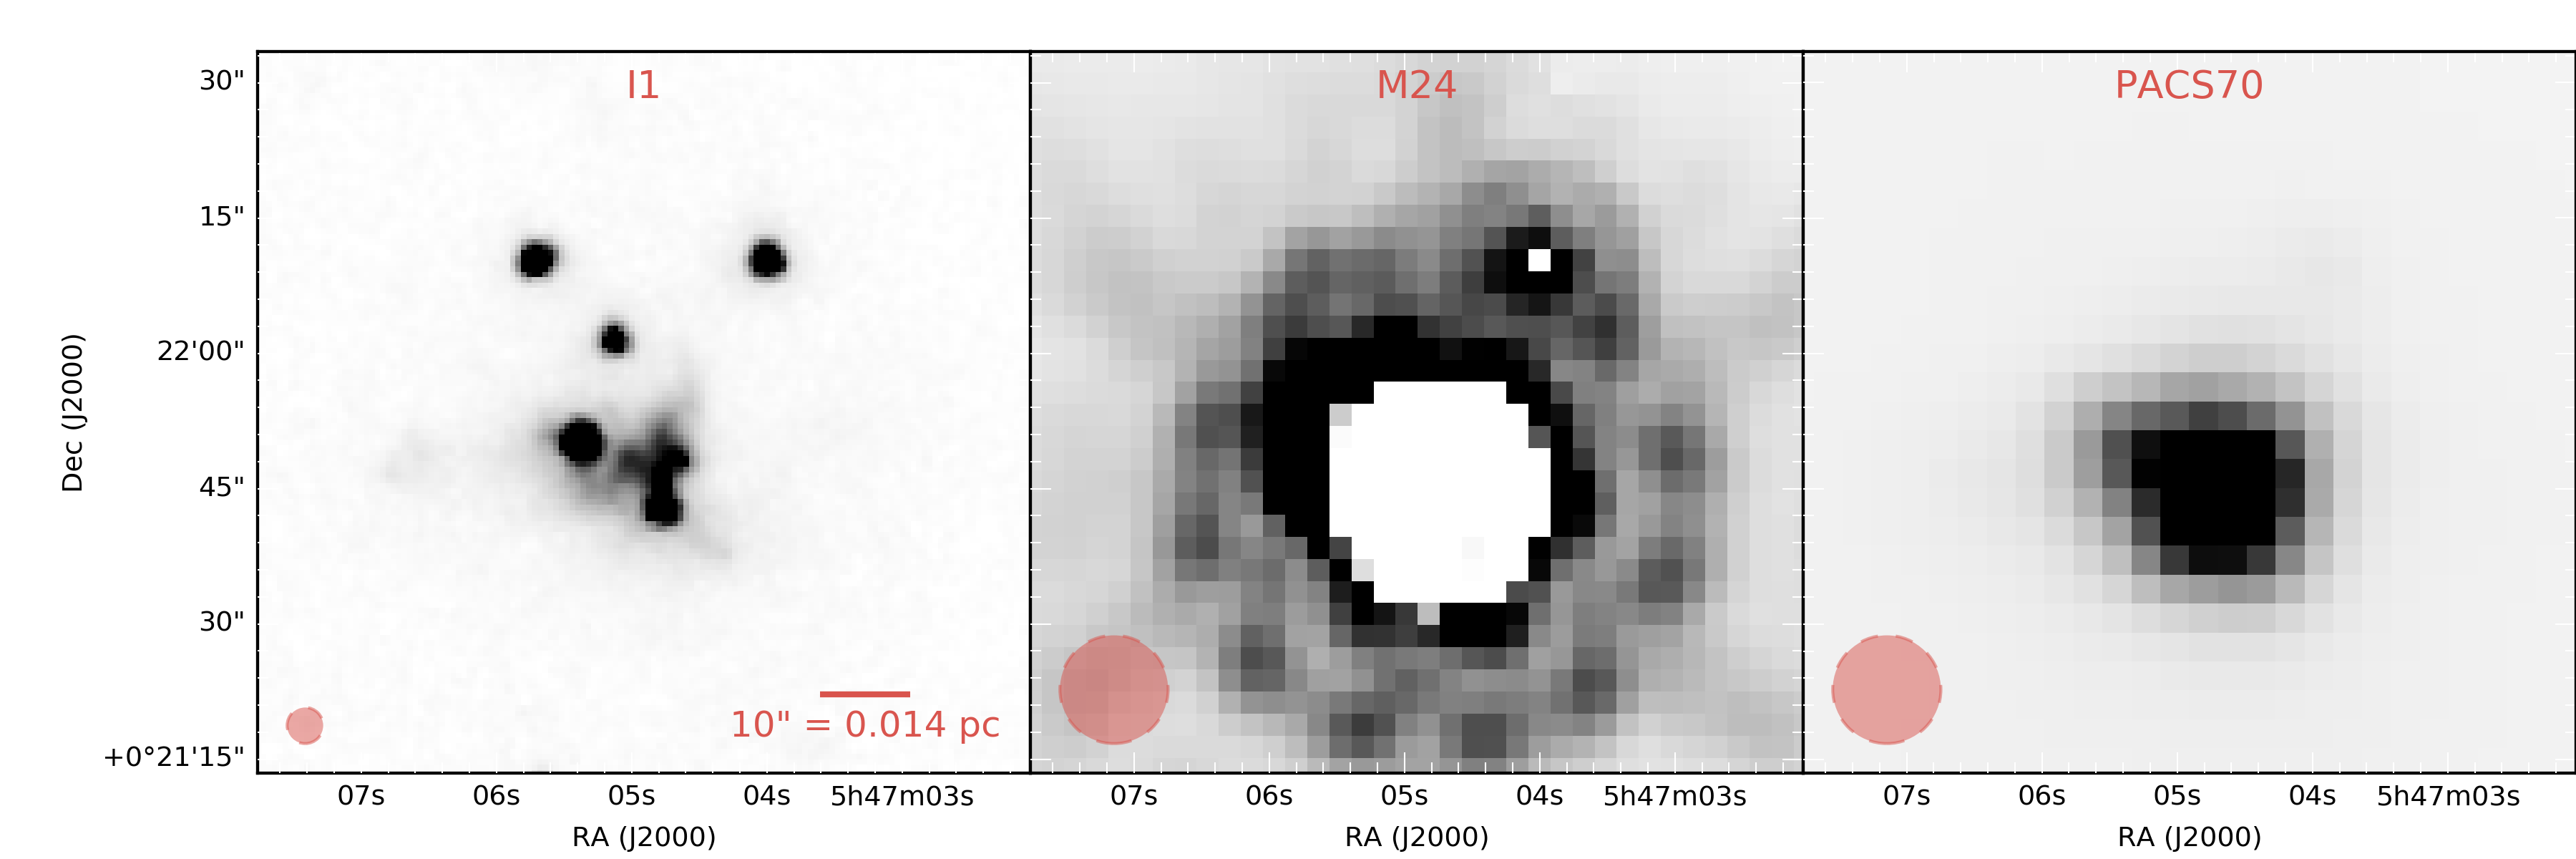
\includegraphics[width=\textwidth]{Figures/NGC2071_saturated_mosaic.png}
\vspace{-0.5cm}
\caption[Saturation and confusion]{Saturation and confusion in NGC2071.}
\label{fig:NGC2071saturated}
\end{center}
\end{figure}

BETTII will tackle the confusion problem at wavelengths from 30 to \SI{100}{\micro\meter}, and will be complementary to \Herschel observations of star-forming regions. SOFIA, however, can already start studying these dense regions with its FORCAST instrument, providing 2-\ang{;;3.5} resolution between 10 and \SI{37}{\micro\meter}. 

We responded to SOFIA FORCAST's first science call with a proposal for a survey of nearby star-forming cluster cores. The clusters were selected from a list of dense young clusters within 1 kpc of the Sun based on \citet{Porras:2003kxa} and \citet{Gutermuth:2009gca}. From this list we selected clusters that were: (1) north of -25 degrees declination so that they could be done from a northern hemisphere flight; (2) included membership of $>$50 YSOs; and (3) included bright 8-\SI{24}{\micro\meter} sources within the dense cores based on \Spitzer and/or WISE data. 

In order to sample the most range of the SED, we proposed to observe in 4 of FORCAST's science continuum bands: 11.1, 19.7, 31.5 and \SI{37.1}{\micron}. This wavelength coverage would be very complementary to archival data from \Spitzer and WISE. Our focus on bright regions spread all across the sky is convenient for SOFIA, and our project would be observed as a gap-filler during the primary science flight legs.

The main objective of the survey is to gather statistics and fill the SED gap between {\Spitzer}'s bands and {\Herschel}'s bands. \Spitzer is often unusable for these targets because of saturation and confusion, and Herschel is confused as well. As it is often the case, \Herschel observations were not available for our targets, making these SOFIA observations the best attempt at observing those regions at mid-IR wavelengths, and our only opportunity to constrain the SED of very clustered YSOs in these regions to infer their physical properties.



Our strategy was successful and we were awarded time during the first and second science cycles of FORCAST (see Tab.~\ref{tab:times}). The data analysis and scientific interpretation is presented in the next few sections. First, we describe our observations, as well as the archival datasets that we use to complement our observations. Second, we properly characterize the systematics of the FORCAST instrument and their variations over multiple science flights spanning multiple years. The data reduction process is then explain, followed by a snapshot of the data products themselves. We then discuss our SED fitting strategy, and fit the SEDs of three of our clusters to derive the physical properties of their embedded YSOs.


\section{Observations}
\label{subsec:SOFIAObservations}

The FORCAST camera has two separate $256\times 256$ pixel infrared arrays that cover the wavelength range from 5.5-\SI{37}{\um} in multiple bands with $\ang{;;0.768}\times\ang{;;0.768}$ pixels. The two arrays can observe simultaneously through a dichroic beam splitter that divides the wavelength range shortward and longward of \SI{26}{\um}. Alternatively, the long wavelength array can be used by itself as the dichroic is removed from the light path, gaining a sensitivity of $\sim 2.5$. We observe the 11.1 and \SI{37.1}{\um} together (hereafter "mode 1") and the 19.7 and \SI{31.5}{\um} together (hereafter "mode 2") . We set the 1$\sigma$ sensitivity threshold to that of a moderately rising SED for a \SI{1.5}{\Lsun} source, which is scaled appropriately for the distance to the cluster. This is an attempt at probing the same luminosities at all distances and obtain a consistent sample of YSOs. 

\renewcommand{\arraystretch}{1.5}
\setlist[itemize,1]{nolistsep,leftmargin=*,labelsep=-\mylen}
\def\labelitemi{--}
\begin{table}[!h]
\scriptsize
\caption{List of desired sensitivities}
\vspace{-0.5cm}
\begin{longtable}{c|cccc|c}
\toprule
Distance & \multicolumn{4}{c|}{1$\sigma$ minimum detectable flux (Jy)} &  Corresponding minimum\\
(pc) & \SI{11}{\um}& \SI{19}{\um}& \SI{31}{\um}& \SI{37}{\um}& \si{\Lsun} \\
\hline
   200.0& 0.1& 0.1& 0.32& 0.7&$\sim$0.5\\
   400.0& 0.1& 0.1& 0.32& 0.6&$\sim$1.5\\
   600.0& 0.05& 0.04& 0.18& 0.25&$\sim$1.5\\
   800.0& 0.02& 0.02& 0.1& 0.12&$\sim$1.5\\
1,000.00& 0.01& 0.01& 0.06& 0.1&$\sim$1.5\\

\bottomrule																																		\end{longtable} 
\caption*{List of desired sensitivities for different distances.}
\label{tab:DesiredSensitivities}
\end{table}



However, for the most nearby clusters, the corresponding observing time was so short that the overhead from the observatory was very costly. Hence, we put a lower threshold to the integration time of \SI{30}{\second}. Similarly, the sensitivity of the \SI{37}{\um} band is such that in order to be consistent with our sensitivity target, this band was heavily driving the  observing time using mode 1. Hence, we observe in this mode as long as is required to meet the sensitivity target for the \SI{11}{\um} band, and request more observations in the \SI{37}{\um} band on its own (hereafter "mode 3"). This allows us to request less total observing time while keeping our sensitivity self-consistent. A summary of our target sensitivities for various distances is shown in Table~\ref{tab:DesiredSensitivities}.

Various observing techniques are available to the FORCAST user to deal with background subtraction. The most robust techniques are very costly in terms of overhead for the observatory, so we decided to be audacious and requested the cheapest observing mode: the Chop-Nod-Chop mode (CNC), combined with 9 ditherings for each field, which dramatically helps when co-adding images together. Most of our data was processed by the SOFIA automated pipeline that provided calibrated Level 2 images, except for the data from the first few flights, for which we received the help of one of FORCAST's Principal Investigator, Dr. Joe Adams, who processed the raw data through his own instrument pipeline.

%\begin{figure}[!h]
%\begin{center}
%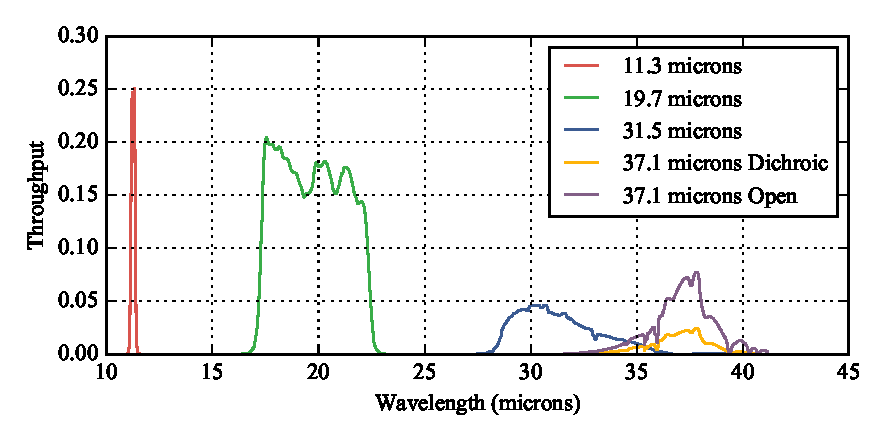
\includegraphics[width=\textwidth]{Figures/SOFIA_bands.pdf}
%\label{fig:SOFIAbands}
%\caption[SOFIA bands]{SOFIA FORCAST bands.}
%\end{center}
%\end{figure}

The data were acquired over 10 SOFIA flights spanning multiple years, with the last batch dating from February 2015. The actual observing times for each band and cluster is shown in Table~\ref{tab:times}. In that table, we have estimated the time for the \SI{37}{\um} band using a composite formula that levels the observing time from mode 3 to that of mode 1, considering their respective sensitivities. We obtained about \SI{10}{\hour} of on-sky data, and 10 out of our 12 original target clusters were observed.

\renewcommand{\arraystretch}{1.5}
\setlist[itemize,1]{nolistsep,leftmargin=*,labelsep=-\mylen}
\def\labelitemi{--}
\begin{table}[!h]
\scriptsize
\caption{List of targets}
\vspace{-0.5cm}
\begin{longtable}{cP{4cm}P{2cm}P{1cm}P{0.5cm}P{0.5cm}P{0.5cm}P{0.5cm}P{0.5cm}}

\toprule																																			
Cluster 	&	 Coordinates 	&	 SOFIA 	&	 $N_\textrm{Fields}$	&	$d $	&	$T_{11} $  	&	$T_{19}  $&	$T_{31}  $&	$T_{37}  $\\
	&	(J2000)	&	Flight IDs	&		&	(pc)	&	(s)	&	(s)	&	(s)	&	(s)	\\
\midrule																	
Cepheus A	&	 22h56m10s +62d03m26s 	&	 F132 F109 	&	2	&	730	&	206	&	234	&	235	&	490	\\
Cepheus C	&	 23h05m45s +62d30m05s 	&	 F132 	&	1	&	730	&	150	&	121	&	121	&	286	\\
IRAS20050	&	 20h07m05s +27d28m51s 	&	 F166 F131 	&	2	&	700	&	321	&	224	&	256	&	266	\\
NGC1333 	&	 03h29m00s +31d17m20s 	&	 F129 F193 F190 	&	9	&	240	&	530	&	558	&	467	&	446	\\
NGC2071 	&	 05h47m06s +00d21m45s 	&	 F192 	&	2	&	420	&	36	&	25	&	33	&	42	\\
NGC2264 	&	 06h41m07s +09d33m35s 	&	 F156 	&	4	&	913	&	495	&	300	&	331	&	587	\\
NGC7129 	&	 21h43m07s +66d06m42s 	&	 F109 	&	1	&	1000	&	383	&	214	&	214	&	709	\\
Ophiuchus 	&	 16h27m05s -24d30m29s 	&	 F157 	&	11	&	150	&	396	&	468	&	501	&	365	\\
S140 	&	 22h19m23s +63d18m44s 	&	 F129 	&	1	&	900	&	322	&	393	&	393	&	568	\\
S171 	&	 00h04m01s +68d34m50s 	&	 F132 	&	1	&	850	&	253	&	219	&	219	&	476	\\\bottomrule																																		\end{longtable} 
\caption*{List of observed targets. For each cluster, we list the SOFIA flights on which the data was taken, the number of individual fields within the cluster, the distance, and the total integration time for each of the 4 observation bands, including all fields. Note that the \SI{37}{\micro\meter} time quote is a composite time calculated by combining the exposure time of mode 1 with that of mode 3, as discussed in the text.}
%List of our 12 proposed targets, with approximate RA and Dec, distance $d$ in parsecs, peak number density in \# stars/pc$^{2}$ from \citep{Gutermuth:2009p1325}, whether the image saturates in Spitzer/in WISE, the number of different fields for each target, the number of YSOs above our threshold level derived from WISE photometry, and the requested time in minutes on source that we request. Note that the latter DOES NOT include overheads.}
\label{tab:times}
\end{table}

To complement our observations, we proceed to an archival search to find publicly available WISE, \Spitzer, and \Herschel images. Most of our targets have already available \Spitzer IRAC and/or MIPS photometry \citep[mostly from][]{Gutermuth:2009gca,Megeath:2012cn,Evans:2009bka}, which we use in the relevant cases. In the cases where no IRAC photometry was available, we applied our own photometry algorithms. We could not find published photometry for the targets with available \Herschel images, hence we also used our own photometry pipeline to derive fluxes. In some cases, we find previously published \SI{1.3}{\milli\meter} continuum measurements to help constrain the long-wavelength behavior of the SEDs.


\section{FORCAST characterization}

In addition to the raw images, a number of calibrators were observed during each flight for different dichroic settings and wavelength bands. These calibrators are usually bright stars which guarantee to be point sources for SOFIA's angular resolution, and have very predictable mid-IR fluxes, so they can be used both for flux and PSF calibration. We use them for two purposes: the first is to obtain a robust metric to determine whether sources are extended or not; the second is to determine the aperture correction factor which will later be used for aperture photometry. 

\subsection{PSF size}
The size of the PSF can be defined in multiple ways, we adopt the approach of characterizing the PSF using its encircled energy distribution. Fig~\ref{fig:averageEE} shows the average of the normalized encircled energy distribution of the PSF, measured on all the calibrators of our sample. Each curve represents one of the five different combinations of bandpass filter and dichroic setting that we use for our observations. For each radius, the total energy is the sum of the pixels within the circular aperture of that radius, to which we subtract an estimate of the background in an annulus around the source (see Section [] for details on the background subtraction methods). 

\begin{figure}[!h]
\begin{center}
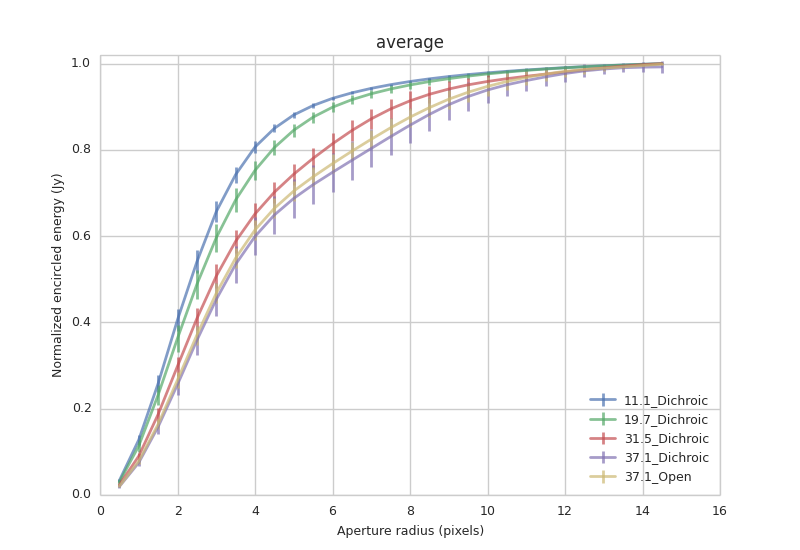
\includegraphics[width=\textwidth]{Figures/average.png}
\vspace{-0.5cm}
\caption[PSF size]{Average PSF encircled energy distribution profile for all calibrator observations.}
\label{fig:averageEE}
\end{center}
\end{figure}


As expected, the PSF at \SI{37.1}{\micro\meter} is larger than the PSFs at shorter wavelengths, but less that the traditional diffraction limit rule. This indicates that additional PSF smearing is occurring at short wavelengths, likely due to plane jitter and pointing errors, which is consistent with what other authors have found \citep[e.g.][]{Herter:2013by}. Throughout all the flights, point source calibrators always have the same encircled energy distribution shape within $\sim 4\%$ rms. 

To look at the behavior of the PSF in more detail, we can use the half width at half maximum of the encircled energy distribution, \Rfifty as a proxy for PSF size. The variation of this quantity for the various flights, bandpass/dichroic setting, and calibrators used is showed in Fig.~\ref{fig:Rfiftydist}. This shows the flight-to-flight differences and, for some calibrators, the in-flight variability. We find that the latter is usually small, except for the SOFIA flight on 05-02-2014, for which the spread is quite considerable and could have been caused by instrumental malfunction or abnormal levels of jitter. The variation from flight to flight is larger than the variation within a given flight, which indicates variability in the observing conditions, systematics, or thermal radiation environment of the observatory between different flights. Even considering the flight-to-flight and calibrator-to-calibrator variations, the overall spread in \Rfifty for a given observation setting is almost always less then 10\%, making this metric a useful reference to compare with scientific data. In our analysis we will compute \Rfifty for our sources and compare it to the \Rfifty from the current flight for the same filter setting, if the calibration file exists. If no calibration file exists for a given setting, we use the mean \Rfifty for that setting from calibrators observations in other flights. The ratio \Rpercent of these two quantities helps quantify the extension of the source, to within $\sim 10\%$. 

\begin{figure}[!h]
\begin{center}
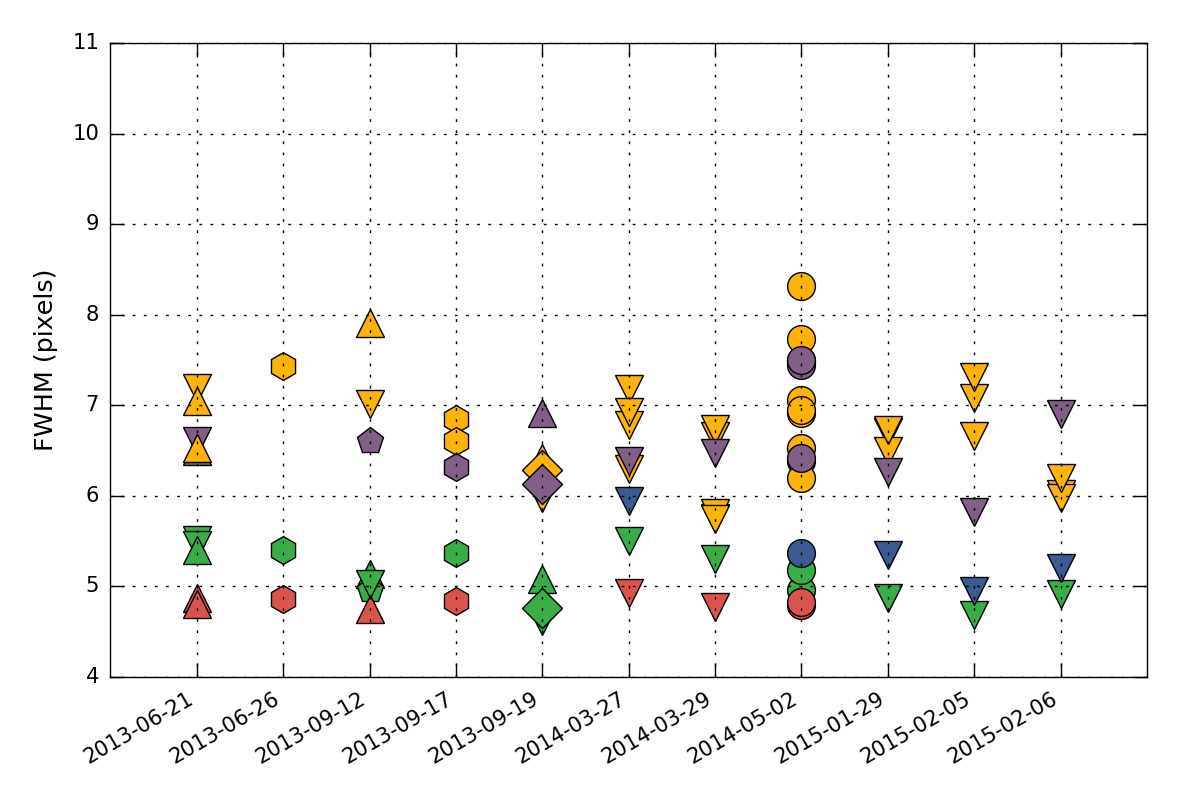
\includegraphics[width=\textwidth]{Figures/R50.png}
\vspace{-0.5cm}

\caption[PSF size of calibrators]{Distribution of \Rfifty for all calibrators observations within each bandpass. In red: \SI{11}{\um} band, with dichroic; in green: \SI{19}{\um} band, with dichroic; in blue: \SI{31}{\um} band, with dichroic; in yellow: \SI{37}{\um} band, with dichroic; in purple: \SI{19}{\um} band, with dichroic. Down triangles: $\alpha$ Boo; Pentagons: $\alpha$ Cet; Diamonds: $\alpha$ Tau;  Up triangles: $\beta$ And; Hexagons: $\beta$ Peg; Circles: $\beta$ UMi;}
\label{fig:Rfiftydist}
\end{center}
\end{figure}

\subsection{Aperture correction factor}
\label{subsec:apcorr}
In Fig.~\ref{fig:averageEE}, we observe that the encircled energy does not vary much by the time the aperture reaches a radius of 12 pixels, so we consider this fiducial aperture as our "total flux" aperture. The goal of aperture photometry is to estimate the amount of flux in this large aperture, which we consider to be the total amount of flux from the source, by only measuring flux within a much smaller aperture. This has the advantage of reducing contamination from other sources, and increases the signal-to-noise ratio of the flux estimate since the pixels near the tail of the PSF usually contain more noise than signal. 
In Fig~\ref{fig:response}, we plot the aperture correction factor that we compute from the ratio of the flux measured within an aperture of 3 pixels radius and this 12-pixel aperture.  Not surprisingly, this graph follows very closely the plot of $\Rfifty$ from Fig~\ref{fig:Rfiftydist}, showing the close link between the aperture correction factor and the shape of the calibrator's PSF. We match each observation in our data to the mean of the aperture correction factors for the same observation setting and flight.

\begin{figure}[!h]
\begin{center}
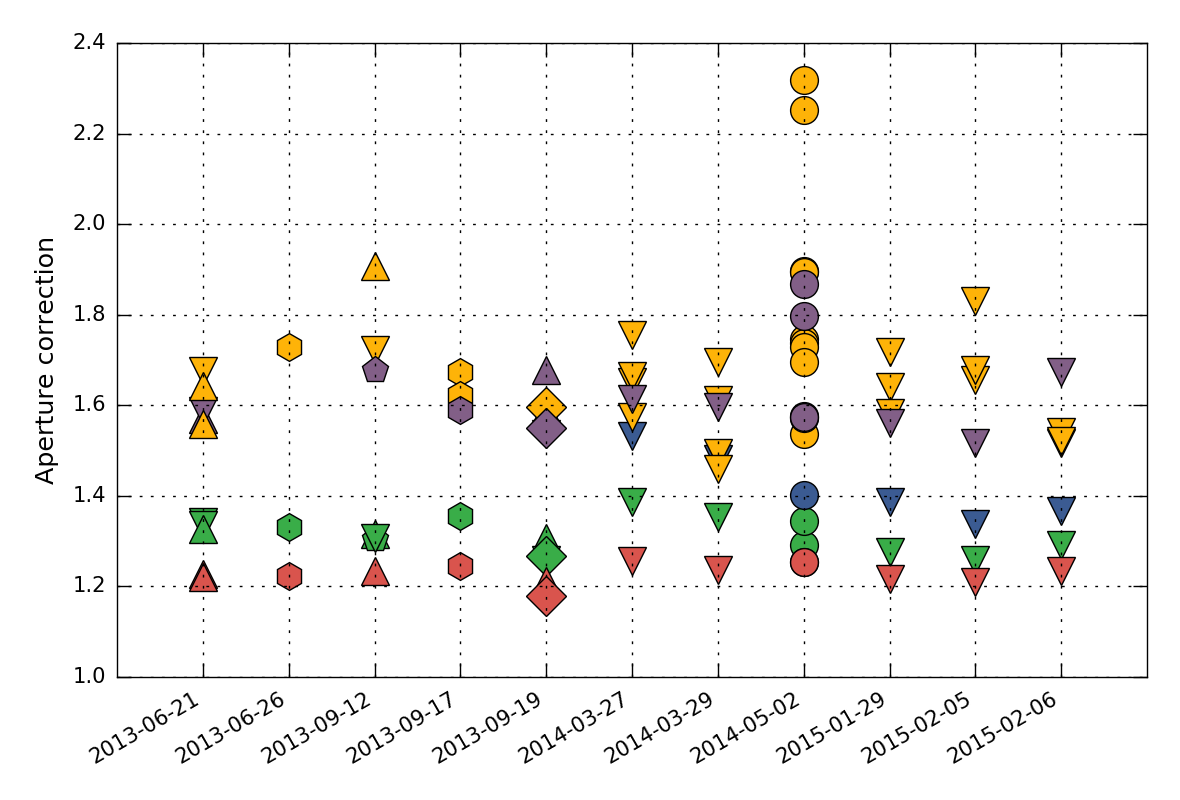
\includegraphics[width=\textwidth]{Figures/Aper_corr.png}
\vspace{-0.5cm}
\caption[aperture correction]{Instrumental response and aperture correction}
\label{fig:apercorr}
\end{center}
\end{figure}



\subsection{Instrument response and overall uncertainty}
To validate our approach, we take a look at the calibrator fluxes after normalization by the calibration factor, which is provided directly by the FORCAST pipeline. This calibration factors converts the pixel digital value a physical flux density unit, and presumably is determined using the flux from calibrator stars as well. Here we re-measure the flux from each calibrator for each observation setting and each flight, using our standard aperture photometry method and background subtraction. Ideally, we would always obtain the same flux for each setting and calibrator, independently of the flight, an assertion we find true to within $\sim 5\%$. The in-flight errors are typically lower than this. This validates our aperture photometry method, and we can trust that the instrument's systematics are well-behaved to within these levels. 

This would suggest that we can adopt systematic $1\sigma$ uncertainties of $\sim 5\%$, a value which is consistent with the published uncertainties of $3\sigma \approx 20\%$ \citep{DeBuizer:2012ie}.


\begin{figure}[!h]
\begin{center}
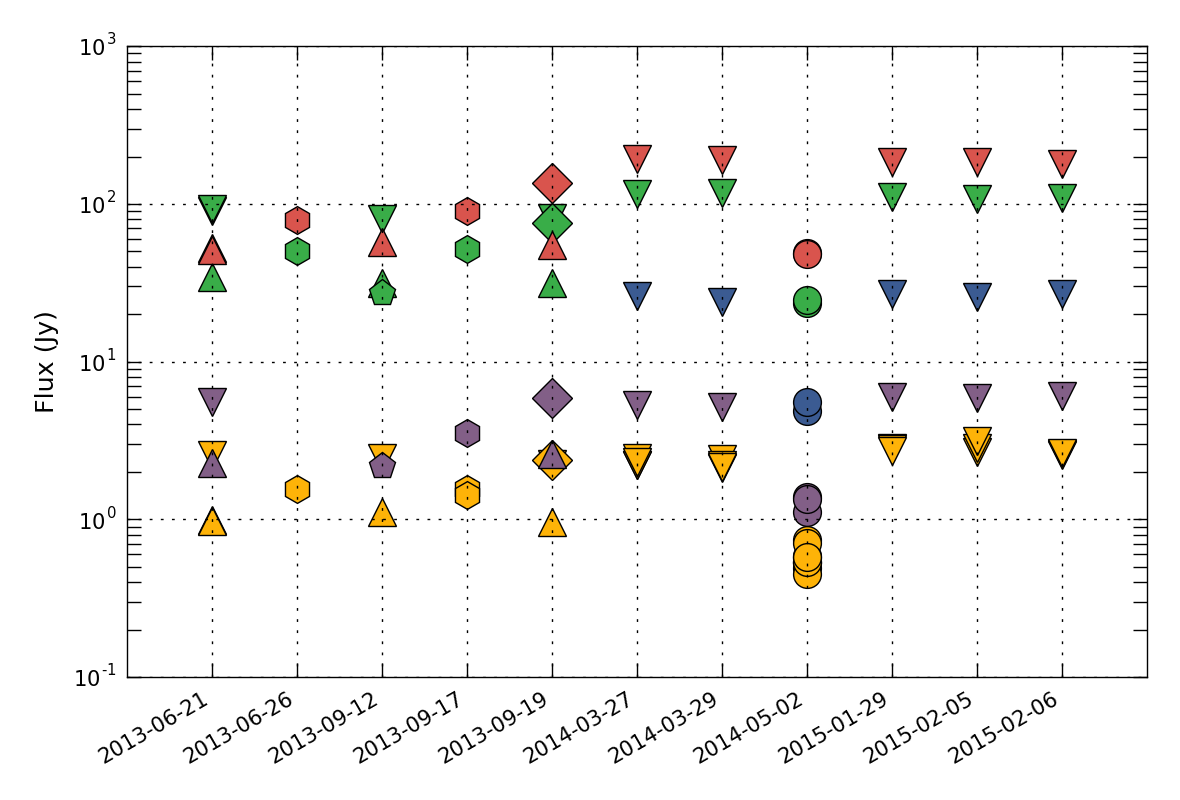
\includegraphics[width=\textwidth]{Figures/Phot_val.png}
\vspace{-0.5cm}
\caption[Instrumental response]{Instrumental response}
\label{fig:response}
\end{center}
\end{figure}




\section{Data reduction and photometry}

The data are processed through various versions of the online pipeline to yield Level 2 data products available on the archive \citep{Herter:2013by}. We apply our own reduction procedure and photometry pipeline on those products to derive final images, source positions, fluxes and sensitivities. Our software makes extensive use of the Python \textit{astropy} package \citep{2013A&A...558A..33A} and its associated modules \textit{photutils} and \textit{APLpy}. 

\subsection{Pre-treatment}
Some manual treatment of each image is necessary before it can be analyzed by our software, which follows this procedure: a) visually aligning the WCS coordinate system, often 10-20" off, using point sources and archival data from other wavelengths and facilities such as IRAC \SI{8}{\micro\meter}; b) cropping the images to clean off the nodded fields, and c) identify the coordinates of each source, both point-like and extended.

After these manual steps, the Level 2 images are multiplied by the calibration factor provided by the online pipeline, which converts them to Jy/pixel. We do not proceed to any systematic color correction, but the effects on the fluxes are very small \citep{Herter:2013by}.
\begin{enumerate}
\item Adjust WCS coordinates: use images at other wavelengths (2MASS, IRAC, MIPS, WISE) to re-align the (RA, DEC) position of the field. We estimate that this process is good to within one SOFIA pixel (\ang{;;0.768}) for the fields where one or more point sources can be identified. Extended fields are less trustworthy, since matching the extended emission to other wavelengths is harder. The rotation of the field produced by the SOFIA pipeline is correct for all of our data. 
\item Crop each image, remove chopped fields, remove artifacts.
\item Identify and categorize sources: isolated point sources, clustered point sources, and extended sources. For extended sources, a circular or elliptical aperture is used to try to encompass the entirety of the emission.
\item Manually identify a location in the field that corresponds to a representative background.
\end{enumerate}

\subsection{Source flux extraction}

We feed the adjusted FITS and associated metadata files to our photometry pipeline. For each identified source, we determine its flux in all bands using aperture photometry with local background subtraction. The aperture correction factor we use is the one determined from the calibrators observed for the same observation setting during the same flight as the one when the data was taken. If a calibrator is not available during the flight, we use the average aperture correction factor taken over 9 of our 10 flights (we choose to exclude the flight on 05/02/2014 which seems to have abnormal behavior).

We distinguish between 3 types of sources after manual identification: \textit{isolated}, which are point sources with no nearby objects; \textit{clustered}, which are point sources with nearby objects; and \textit{extended}, which are not consistent with being point sources. 

For point sources that are isolated, we use our standard aperture of 3 pixels at all wavelengths. We consider an annulus surrounding the source extending from 12 to 20 pixels radius (24 to 40 for clustered sources): the local background is determined from the mode of the pixels in the annulus, while the sensitivity is calculated by measuring the standard deviation of the flux values within 4-pixel apertures spread over that annulus \citep{Shimizu:2016if}. We apply the aperture correction derived from the calibrator observations taken during that flight.

For extended sources, an elliptical aperture is determined manually from the \SI{37}{\micro\meter} images. The local background is determined from the mode of an elliptical annulus, with an inner boundary at the elliptical aperture and an outer boundary corresponding to an ellipse 20\% larger. The sensitivity quoted is the point source sensitivity, and is determined following the same method as for point sources, using the standard deviation of apertures spread across the elliptical annulus. 

The photometry from sources that were observed in different flights is then combined to increase the signal-to-noise ratio. This combination takes into account the sensitivity of each source by appropriately weighing each image.

The source sensitivity calculated is added to the systematic uncertainty of the instrument, for which we follow the recommendation from \citep{Herter:2012hv} to adopt a 7\%, $1\sigma$ uncertainty. 

\renewcommand{\arraystretch}{1.5}
\setlist[itemize,1]{nolistsep,leftmargin=*,labelsep=-\mylen}
\def\labelitemi{--}
\begin{table}[!h]
\scriptsize
\caption{SOFIA photometry comparison} \label{tab:SOFIAPhotometryHarvey}
\vspace{-0.5cm}
\begin{longtable}{l|P{1cm}P{1cm}P{1cm}P{1cm}P{1cm}P{1cm}P{1cm}}
\toprule															
SOFIA name	&	F11	&	F11L	&	F19	&	F31	&	F31L	&	F37	&	F37L	\\
	&	Jy	&	Jy	&	Jy	&	Jy	&	Jy	&	Jy	&	Jy	\\
\midrule															
S140.3	&	10.28	&	9.70	&	101.49	&	419.41	&	401.00	&	525.90	&	669.00	\\
S140.4	&	3.80	&	4.00	&	88.95	&	337.22	&	368.00	&	352.07	&	485.00	\\
S140.5	&	110.57	&	110.00	&	830.97	&	2065.13	&	1585.00	&	2278.61	&	2176.00	\\
\midrule															
Sum of sources in cluster	&	124.65	&	123.70	&	1021.40	&	2821.76	&	2354.00	&	3156.58	&	3330.00	\\
Total cluster emission	&	135.20	&	145.00	&	1194.57	&	4449.46	&	3780.00	&	5840.64	&	6730.00	\\
Ratio	&	1.08	&	1.17	&	1.17	&	1.58	&	1.61	&	1.85	&	2.02	\\
\bottomrule					
	\end{longtable} 
\caption*{Comparison of SOFIA four-band photometry from \citet{Harvey:2012kw} on S140 (columns with 'L'). All fluxes are in Janskies. The authors' "total emission" actually represents the total emission in the entire field of view, whereas out measurement corresponds to a manually-selected source region encompassing only the dense core. The total emission in the entire field of view is less representative, as it could include contribution from other sources as well as areas of negative flux from the chopping and nodding steps. In this cluster, there is a large amount of emission which is not due to the three identified sources.}

\end{table}


To validate our flux extraction method, we compare our results with data from \citet{Harvey:2012kw} who observed one of the sources in our sample, S140. Their photometry (shown in their Table 1) of IRS 1, 2 and 3 (respectively corresponding to our targets S140.5, S140.4, and S140.3) is compared to our photometry in Table~\ref{tab:SOFIAPhotometryHarvey}. We find very good agreement between our fluxes and theirs. The remaining differences can always be explained by slight differences in the center location of the aperture.


\subsection{Image sensitivity}


\renewcommand{\arraystretch}{1.5}
\setlist[itemize,1]{nolistsep,leftmargin=*,labelsep=-\mylen}
\def\labelitemi{--}
\begin{table}[!ht]
\scriptsize
\caption{FORCAST Sensitivities}
\vspace{-0.5cm}
\begin{longtable}{c|P{0.5cm}P{0.5cm}P{0.5cm}|P{0.5cm}P{0.5cm}P{0.5cm}|P{0.5cm}P{0.5cm}P{0.5cm}|P{0.5cm}P{0.5cm}P{0.5cm}|P{1cm}}
\toprule																			
Cluster 	&	\multicolumn{3}{c|}{F11}					&	\multicolumn{3}{c|}{F19}					&	\multicolumn{3}{c|}{F31}					&	\multicolumn{3}{c|}{F37}					&	 Sources 	\\
	&	$\sigman$ 	&	$\sigstd$ 	&	$\sigth$	&	$\sigman$ 	&	$\sigstd$ 	&	$\sigth$	&	$\sigman$ 	&	$\sigstd$ 	&	$\sigth$	&	$\sigman$ 	&	$\sigstd$ 	&	$\sigth$	&		\\
\midrule																											
CepA 	&	0.07	&	0.04	&	0.05	&	0.11	&	0.05	&	0.05	&	0.19	&	0.07	&	0.16	&	0.26	&	0.09	&	0.34	&	4	\\
CepC 	&	0.03	&	0.03	&	0.04	&	0.10	&	0.05	&	0.04	&	0.19	&	0.06	&	0.16	&	0.16	&	0.09	&	0.30	&	4	\\
IRAS20050 	&	0.04	&	0.03	&	0.04	&	0.08	&	0.04	&	0.05	&	0.13	&	0.05	&	0.16	&	0.30	&	0.11	&	0.32	&	7	\\
NGC1333 	&	0.12	&	0.04	&	0.07	&	0.07	&	0.07	&	0.07	&	0.22	&	0.08	&	0.25	&	0.48	&	0.13	&	0.52	&	11	\\
NGC2071 	&	0.19	&	0.10	&	0.12	&	0.32	&	0.15	&	0.15	&	0.21	&	0.22	&	0.49	&	0.45	&	0.28	&	0.81	&	6	\\
NGC2264 	&	0.07	&	0.03	&	0.05	&	0.19	&	0.05	&	0.06	&	0.28	&	0.07	&	0.20	&	0.21	&	0.09	&	0.43	&	21	\\
NGC7129 	&	0.07	&	0.03	&	0.03	&	0.10	&	0.04	&	0.03	&	0.26	&	0.09	&	0.12	&	0.17	&	0.08	&	0.19	&	5	\\
Ophiuchus 	&	0.11	&	0.05	&	0.08	&	0.16	&	0.07	&	0.08	&	0.31	&	0.09	&	0.27	&	0.41	&	0.18	&	0.65	&	19	\\
S140 	&	0.04	&	0.03	&	0.03	&	0.16	&	0.03	&	0.03	&	0.21	&	0.07	&	0.09	&	0.35	&	0.11	&	0.21	&	7	\\
S171 	&	0.04	&	0.03	&	0.03	&	0.07	&	0.04	&	0.03	&	0.07	&	0.05	&	0.12	&	0.16	&	0.06	&	0.23	&	2	\\
\bottomrule					
	\end{longtable} 
\caption*{For each band, we measure the 1$\sigma$ sensitivity \sigman and \sigstd in each field from the data using two different methods (see text), and present here the median of all fields. The theoretical sensitivity \sigth corresponds to the expected sensitivity for the actual integration time, using the SOFIA FORCAST observation planning tools and assuming moderate water vapor content. All sensitivity values are in Janskies.}
%List of our 12 proposed targets, with approximate RA and Dec, distance $d$ in parsecs, peak number density in \# stars/pc$^{2}$ from \citep{Gutermuth:2009p1325}, whether the image saturates in Spitzer/in WISE, the number of different fields for each target, the number of YSOs above our threshold level derived from WISE photometry, and the requested time in minutes on source that we request. Note that the latter DOES NOT include overheads.}
\label{tab:SOFIASensitivity}
\end{table}

In order to determine the absolute sensitivity in the image, we use two methods. First, we manually determine a region in each cluster that visually appears devoid of flux. We calculate the sensitivity as if this background region was a source, by patching apertures in an annulus around this background location and calculating the standard deviation of the obtained fluxes. We call this sensitivity measurement $\sigman$. The main downside of this method is that it requires a manual operation to select the appropriate background field, and hence could have more variation depending on which field we select. Second, we use a routine that iteratively isolates the pixel values above $2\sigma$ of the image, in order to remove the contamination from our actual sources. The standard deviation of the resulting image is then calculated, and is multiplied by the square root of the number of pixels in an aperture of 3 pixel radius. This corresponds to a floor sensitivity $\sigstd$. We present our results in Table~\ref{tab:SOFIASensitivity}, where we also compare this sensitivity with the expected sensitivity $\sigth$ obtained using the online calculator with the actual exposure time of our images. We note that usually, the theoretical values are more in agreement with our first method. 



\subsection{Other photometry}

While SOFIA provides mid-IR photometry, we looked in the literature for published fluxes on our targets in order to reconstruct more complete SEDs. In addition to our four SOFIA bands, our table includes data from 2MASS, \Spitzer, and other instruments. Photometry from these sources is published in online catalogs, which we programmatically cross-reference with the positions of our targets. The closest target that corresponds to a Vizier location query is selected to be the correct catalog match. For the 2MASS data, the location of the target needs to be less than \ang{;;2} away from our coordinates for point sources, and \ang{;;5} for extended sources. For the \Spitzer data, the matching radius is \ang{;;3} for point sources and \ang{;;10} for extended sources. In addition to automated online catalog searches, we also add values for sources in NGC2071 from \citet{vanKempen:2012fb}.

For our two most clustered cases in the cores of NGC2071 and IRAS20050+2720, the published catalogs do not have all available fluxes. We assume that the sources are so clustered that they the source extraction software from these authors do not register them as point sources, due to confusion or saturation effects. Hence we adapt our own photometry routines for these clustered environments and obtain the fluxes directly from the calibrated Level 3 images themselves, which are all available on the archive. In Table~\ref{tab:SpitzerPhotometry}, we compare our photometry results with published fluxes from \citet{Megeath:2012cn} and \citet{Gutermuth:2009gca} for isolated sources elsewhere in these same fields of view. We use the \Spitzer handbook recommendations for aperture photometry on \Spitzer archival images (\ang{;;2.4} aperture with and an annulus that extends from 12 to \ang{;;20}). We find that our results are within 10\% of these other authors' results, which can reflect a simple difference in exact aperture centroiding position. 

\renewcommand{\arraystretch}{1.5}
\setlist[itemize,1]{nolistsep,leftmargin=*,labelsep=-\mylen}
\def\labelitemi{--}
\begin{table}[!h]
\scriptsize
\caption{Spitzer photometry comparison}
\vspace{-0.5cm}
\begin{longtable}{l|P{1cm}P{1cm}P{1cm}P{1cm}}
\toprule																			
SOFIA name	&	i1	&	i2	&	i3	&	i4	\\
	&	Jy	&	Jy	&	Jy	&	Jy	\\
\midrule									
NGC2071.1	&	0.060	&	0.056	&	0.004	&	-0.021	\\
NGC2071.3	&	0.018	&	-0.010	&	-0.004	&	-0.047	\\
NGC2071.4	&	0.090	&	-0.054	&	0.036	&	-0.066	\\
NGC2071.5	&	-0.130	&	-0.109	&	-0.144	&	-0.139	\\
\midrule									
IRAS20050.1	&	0.020	&	0.039	&	0.017	&	0.131	\\
IRAS20050.3	&	0.181	&	0.122	&	0.082	&	0.121	\\
IRAS20050.6	&	-0.044	&	-0.046	&	-0.092	&	-0.056	\\
\bottomrule					
	\end{longtable} 
\caption*{\textbf{Note:} Fractional difference between our own aperture photometry on \Spitzer archival images and published \Spitzer photometry from \citet{Megeath:2012cn} for NGC2071, and \citet{Gutermuth:2009gca} for IRAS20050+2720. When values are negative, it means that their photometry is lower than ours.}
\label{tab:SpitzerPhotometry}
\end{table}

In some cases, we also found archival Herschel images, although no published photometry was available for most our sources. We then apply our same aperture photometry routines for those calibrated Herschel images, using aperture and background subtraction parameters from \citep{Shimizu:2016if} for the PACS and SPIRE. We find also very good agreement between our photometry results for the PACS~\SI{70}{\um} band and the published \Spitzer MIPS~\SI{70}{\um} for some of these sources. %Because of the very large beams of Herschel compared to FORCAST, the SPIRE bands are considered upper limit fluxes for sources that are further than \SI{300}{\pc}.

\section{Data products}

\subsection{Mosaics}
The SOFIA FORCAST archival images consist of $\sim~200$ individual images, each representing a field at a given wavelength. Some fields are revisited multiple times when the entire observation could not happen in a single flight leg. These individual fields are processed and mosaiced together to form one single map for each wavelength and each cluster. 

Before mosaicing the fields, we proceed to a 2D background subtraction. This method divides the images into sections of $50\times 50$ pixels, estimates the median in each cell, and fits a 2D function to these median values. This function is then used to construct a smooth background, which is then completely removed from the image. Each background-subtracted image is then calibrated (using the calibration factor that is supplied by the FORCAST pipeline), and weighed by its exposure time before it is co-added into a mosaic in the WCS coordinate frame. Note that although these maps are useful to take a quick glance at the flux distribution and spot artifacts, the actual photometry described in the previous sections uses each individual raw field, before the mosaicing and without background subtraction. If a source is present in multiple fields, the photometry from each of these fields is combined to provide a better flux estimate.

In Fig.~\ref{fig:varietySources} we present a variety of maps from our cluster sample. Each map is a three-color image (red: \SI{37}{\micron}, green: \SI{31}{\micron} and blue: \SI{19}{\micron}), and the scale and stretch of each color is adjusted to balance each color. 

\begin{figure}[!h]
\begin{center}
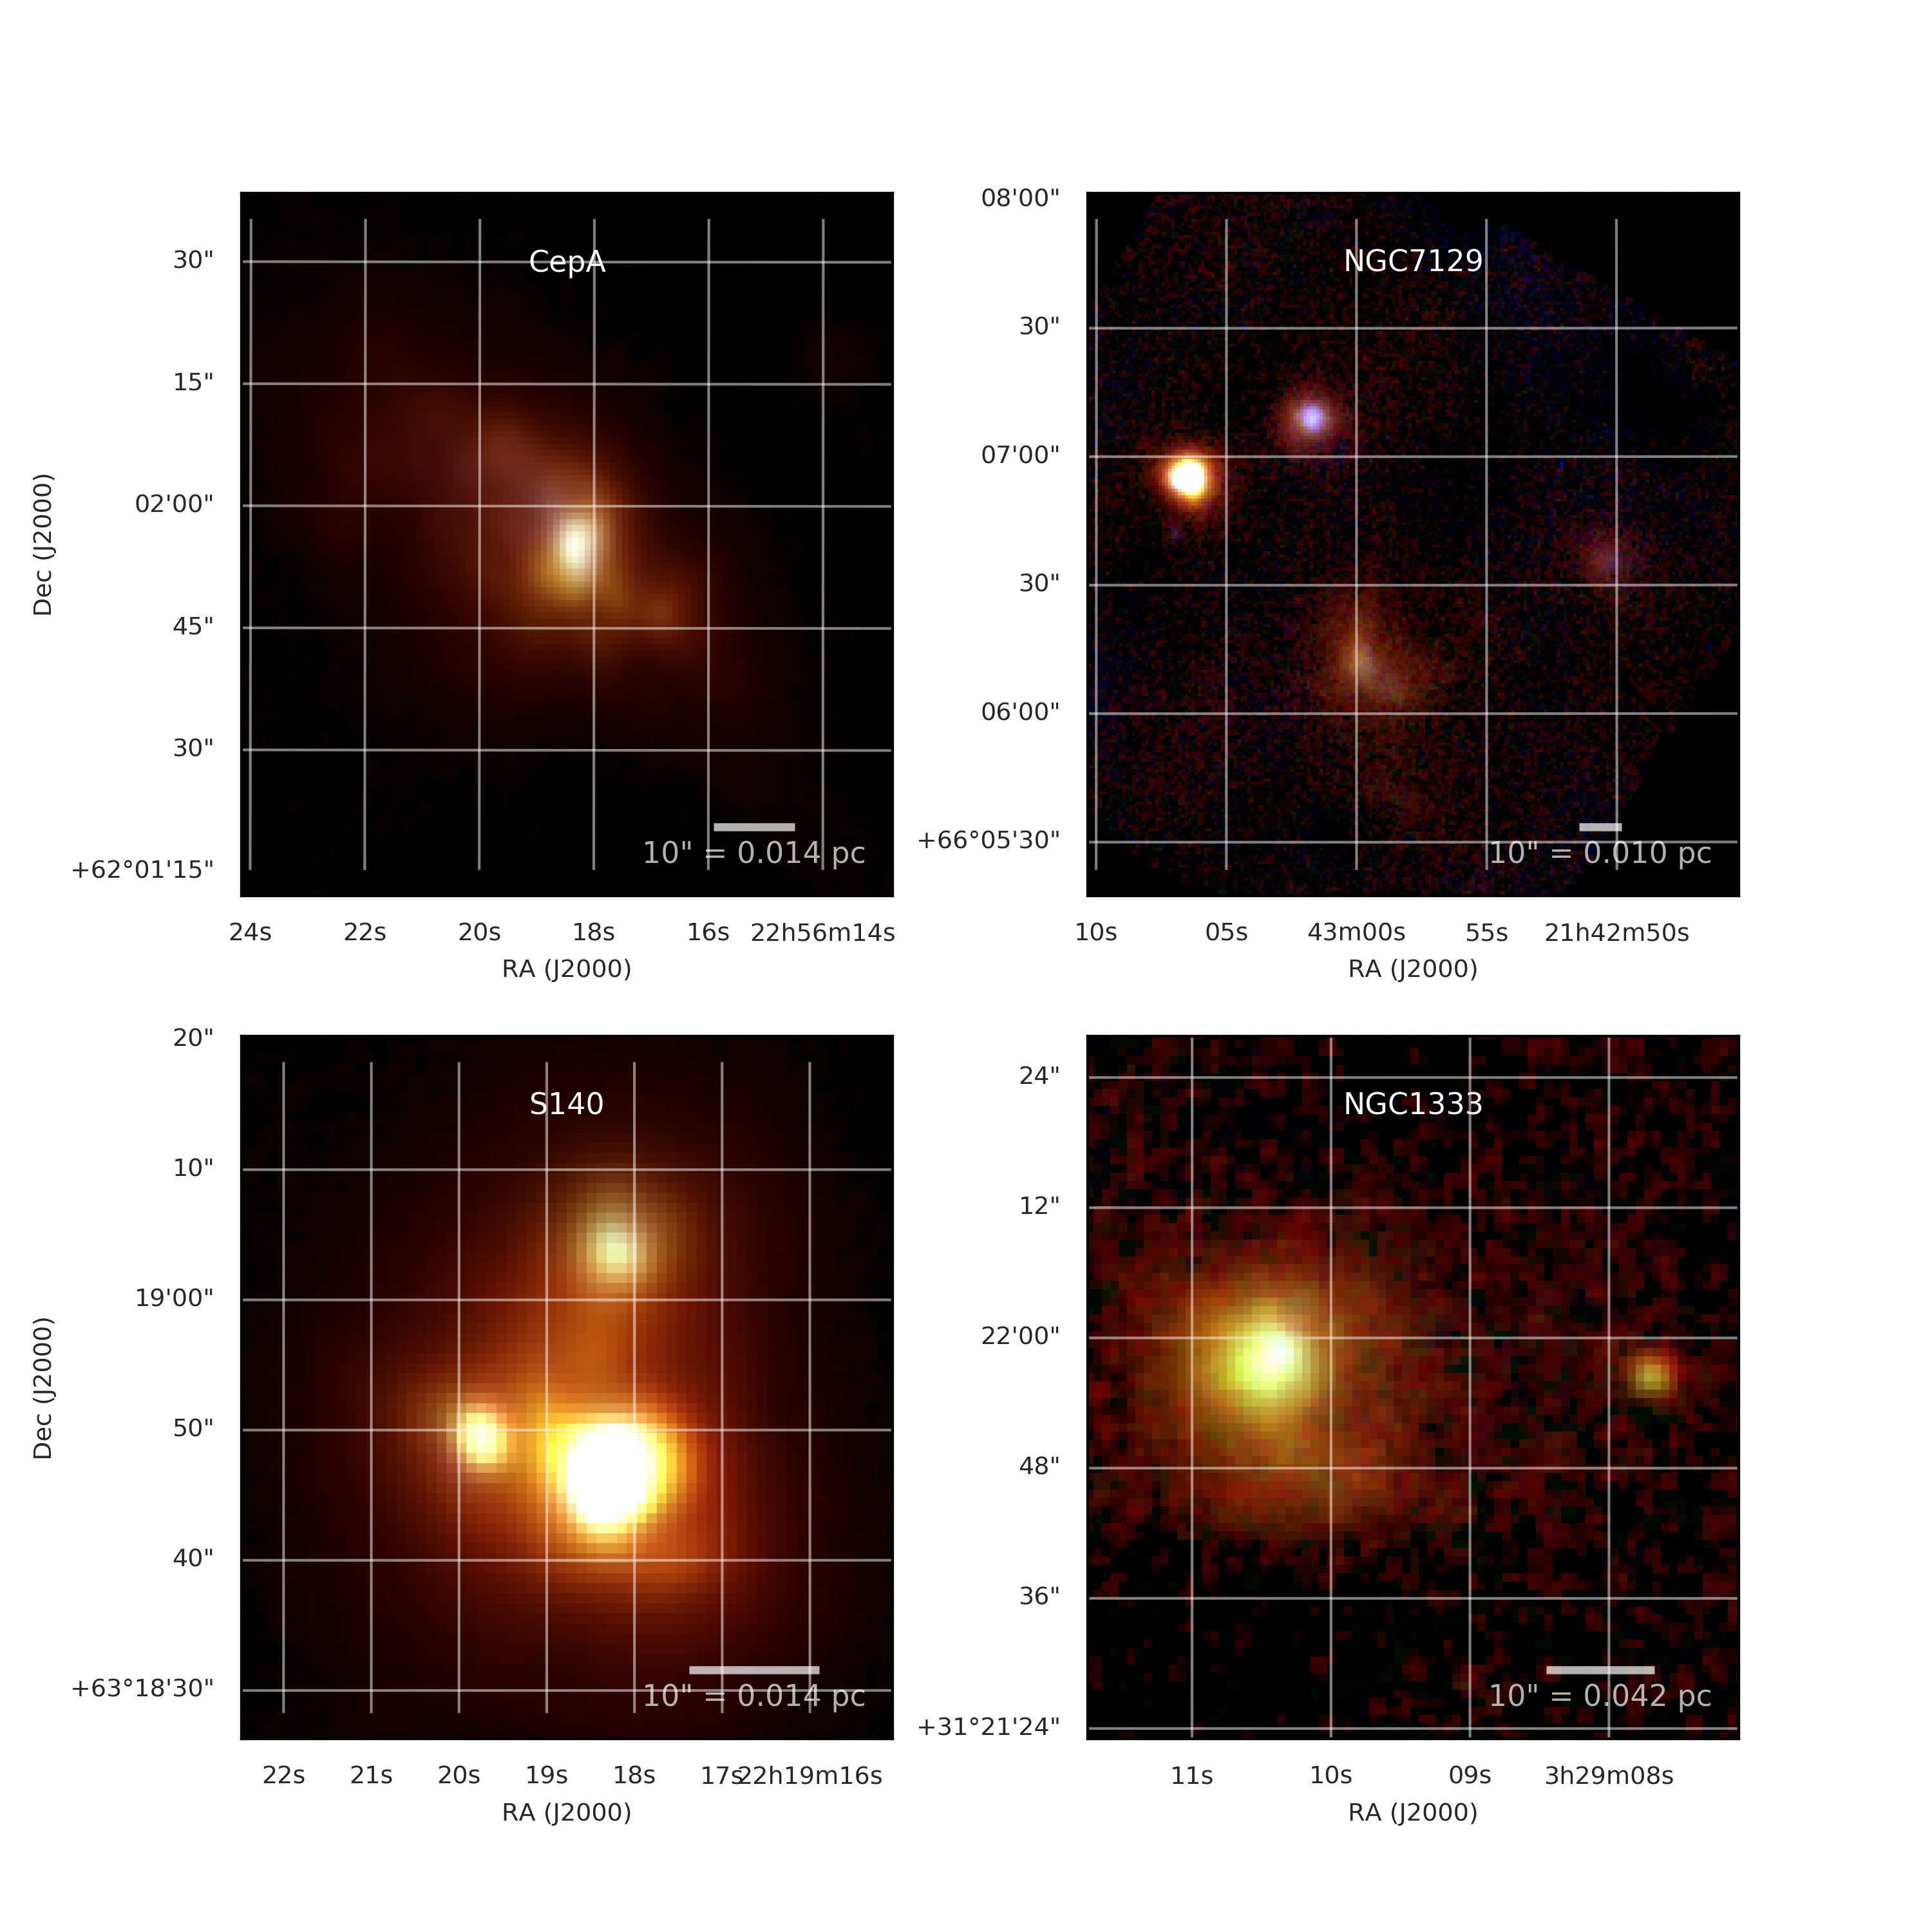
\includegraphics[width=\textwidth]{Figures/RGBmosaic.png}
\vspace{-1cm}
\caption[RGB images of select sample of sources]{Selected sample of sources}
\label{fig:varietySources}
\end{center}
\end{figure}

\subsection{Photometry and SEDs}
%We also produce enhanced SEDs for all of our sources, where we combine archival data with our new SOFIA photometry. The SED plots are complemented with snapshots of the source seen with IRAC and SOFIA. In addition, a snapshot of the corresponding FORCAST \SI{37}{\um} calibrator is shown, which allows to quickly determine the degree of spatial extension of the sources.

The main type of data made available to the community is a list consolidated list of fluxes for most of our clusters, where we gather 2MASS, \Spitzer, FORCAST, \Herschel, SCUBA, and SMA data, when available, for $\sim 90$ sources. Most sources are point sources for the SOFIA FORCAST \SI{37}{\um} band, but some sources present a certain spatial extension which was not known before. 


\begin{figure}
\begin{center}
\hspace*{-1.5in}
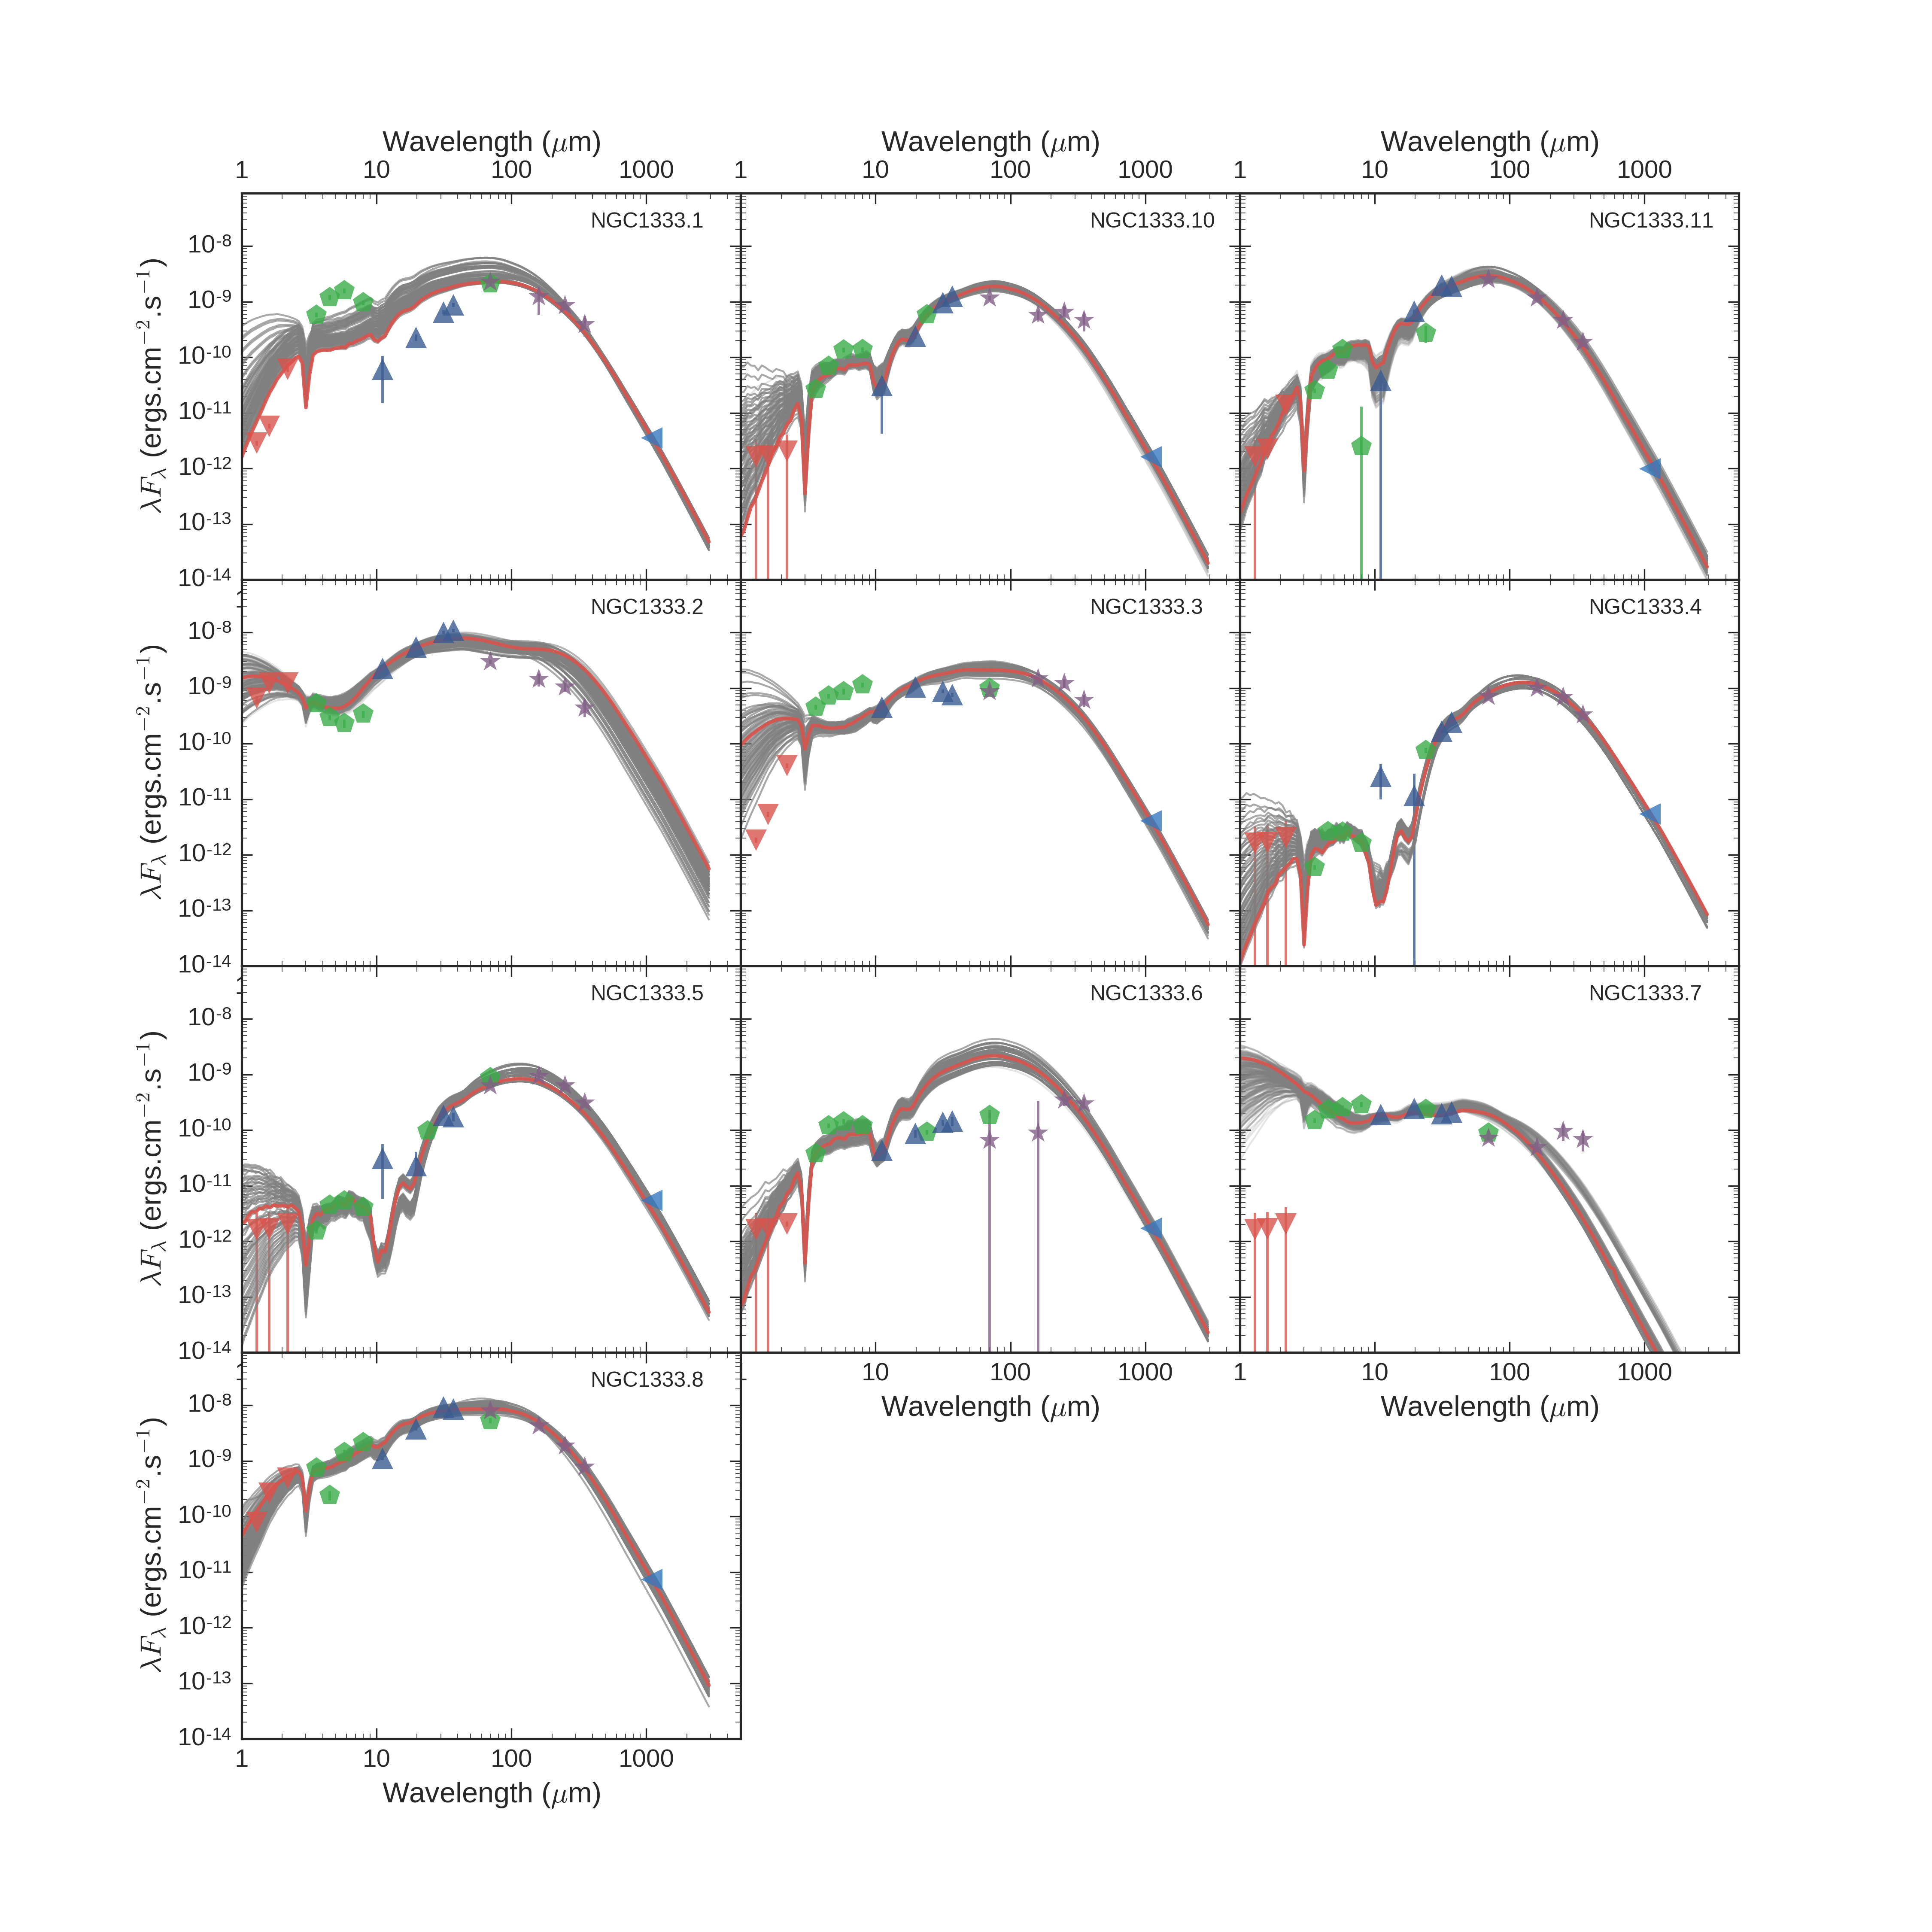
\includegraphics[width=1.4\textwidth]{Figures/NGC1333_SEDs.png}
\caption[NGC1333 SEDs]{SEDs of the point sources in NGC1333. The red curve represents the bet fit. The grey curves represent all the fits with $R$ within 0.5 of the best fit. Red triangles: 2MASS. Green diamonds: \Spitzer (our data or data from other existing catalogs). Dark blue triangles: FORCAST (our data). Purple stars: \Herschel (our photometry). Green triangles: Data from \citep{vanKempen:2009ku} and \citep{vanKempen:2012fb}. Light blue triangles: Data from \citet{Enoch:2009ch}.}
\label{fig:NGC1333_SEDs}
\end{center}
\end{figure}

\begin{figure}
\begin{center}
\hspace*{-1.5in}
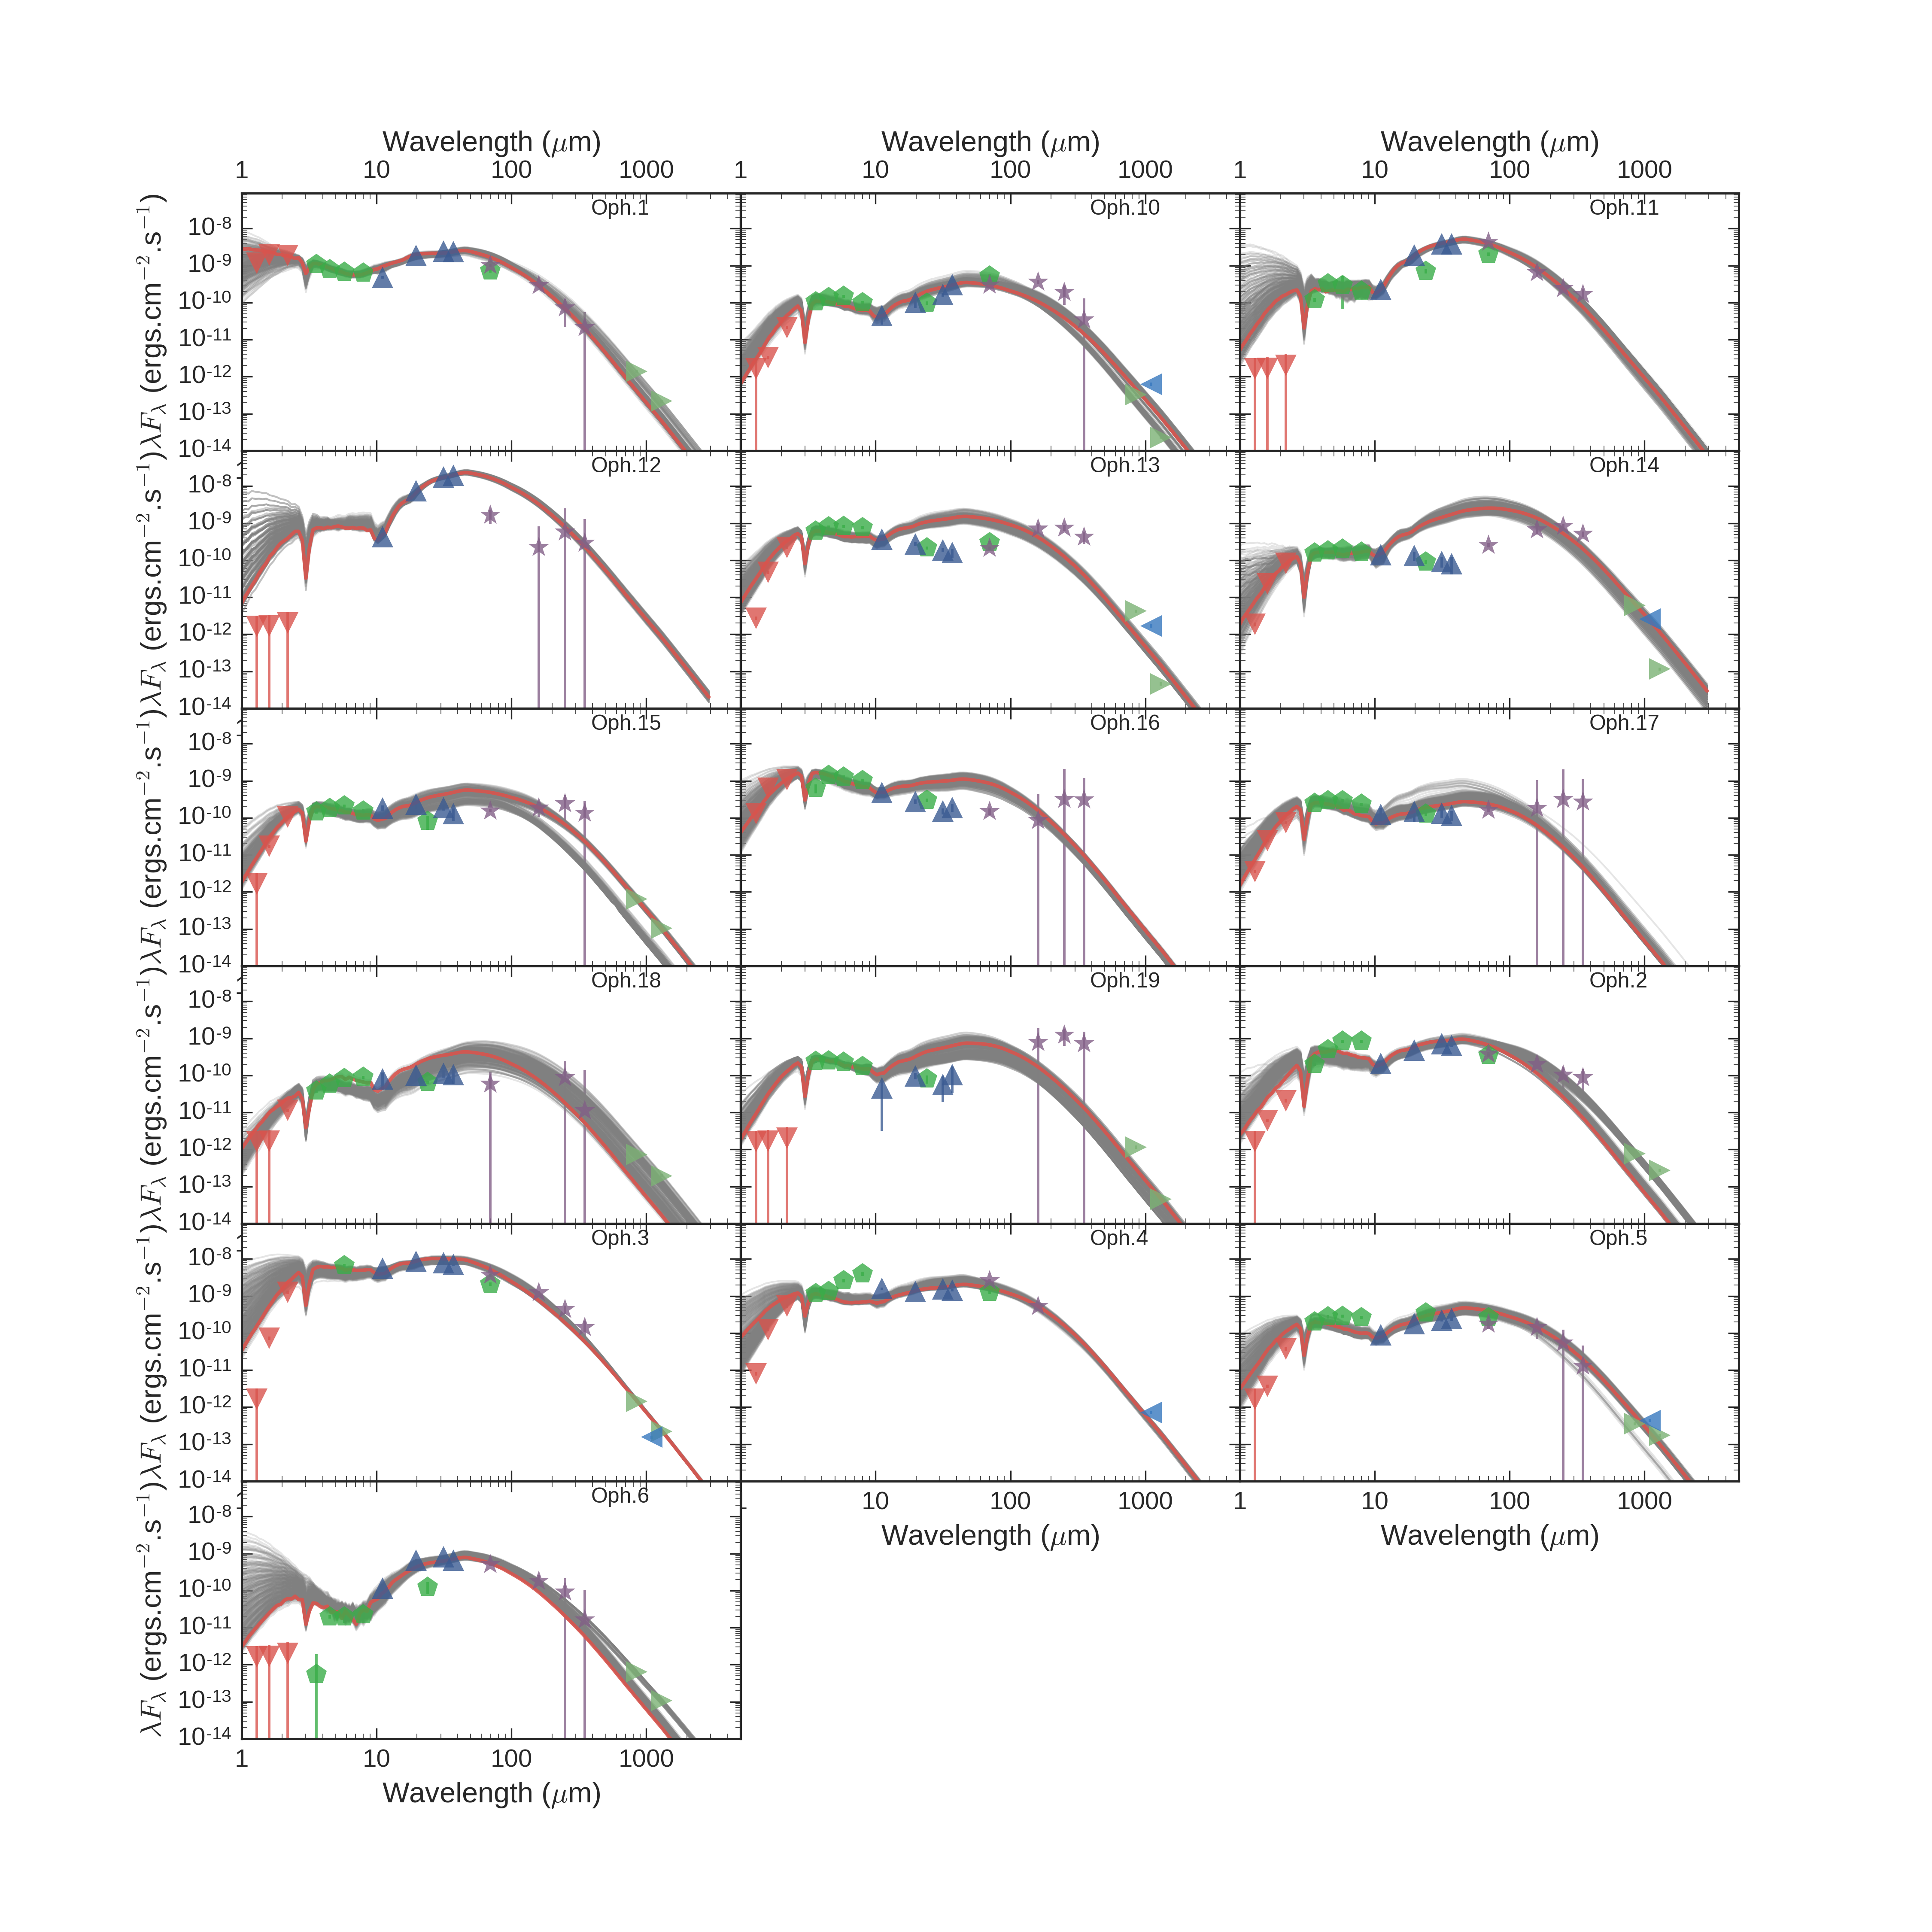
\includegraphics[width=1.4\textwidth]{Figures/Oph_SEDs.png}
\label{fig:Oph_SEDs}
\caption[Ophiuchus SEDs]{SEDs of the point sources in the Ophiuchus cluster. Same legend as Fig.~\ref{fig:NGC1333_SEDs}}
\end{center}
\end{figure}

A few other parameters are determined from the FORCAST data and shown in the data release: the $R_{37}$, which consists of the ratio of \Rfifty for the source and \Rfifty for the last observed calibrator; the spectral index and its uncertainty, computed out of the fluxes from \SI{2.2}{\um} to \SI{37}{\um}; and the bolometric luminosity and temperatures for each source. An excerpt of the final table is shown in Table~\ref {tab:OphiuchusNGC1333}.
\begin{landscape}
\begin{table}[!h]
\tiny
\caption[NGC1333 photometry]{Extract of NGC1333 photometry.}
\label{tab:OphiuchusNGC1333}
\vspace{-0.5cm}
\begin{longtable}{llrrrrrrrrrrrrr}
 \toprule																														
SOFIA name	&	Coordinates		&	R37	&	Lbol	&	Tbol	&	j	&	e\_j	&	h	&	e\_h	&	ks	&	e\_ks	&	i1	&	e\_i1	&	i2	&	e\_i2	\\
\midrule																														
NGC1333.1	&	03h29m07.7s	+31d21m57.0s	&	0.746	&	8.385	&	22.401	&	0.0012	&	0.0001	&	0.0031	&	0.0003	&	0.0450	&	0.004	&	0.696	&	0.070	&	1.800	&	0.180	\\
NGC1333.2	&	03h29m10.3s	+31d21m55.5s	&	2.232	&	27.832	&	24.356	&	0.2853	&	0.0285	&	0.6539	&	0.0654	&	0.9010	&	0.090	&	0.637	&	0.064	&	0.446	&	0.045	\\
NGC1333.3	&	03h29m01.5s	+31d20m20.5s	&	0.904	&	8.104	&	20.630	&	0.0008	&	0.0001	&	0.0029	&	0.0003	&	0.0296	&	0.003	&	0.544	&	0.054	&	1.090	&	0.109	\\
NGC1333.4	&	03h29m11.1s	+31d18m30.8s	&	1.103	&	3.056	&	4.204	&	0.0007	&	0.0007	&	0.0009	&	0.0009	&	0.0015	&	0.002	&	0.001	&	0.000	&	0.004	&	0.000	\\
NGC1333.5	&	03h29m10.6s	+31d18m19.6s	&	1.623	&	2.786	&	4.424	&	0.0007	&	0.0007	&	0.0009	&	0.0009	&	0.0015	&	0.002	&	0.002	&	0.000	&	0.007	&	0.001	\\
NGC1333.6	&	03h29m13.0s	+31d18m13.8s	&	0.951	&	1.155	&	17.248	&	0.0007	&	0.0007	&	0.0009	&	0.0009	&	0.0015	&	0.000	&	0.046	&	0.005	&	0.180	&	0.018	\\
\midrule																														
	&			&	i3	&	e\_i3	&	i4	&	e\_i4	&	F11	&	e\_F11	&	F19	&	e\_F19	&	m1	&	e\_m1	&	F31	&	e\_F31	&	F37	\\
\midrule																														
NGC1333.1	&	03h29m07.7s	+31d21m57.0s	&	3.060	&	0.306	&	2.550	&	0.255	&	0.225	&	0.169	&	1.502	&	0.208	&	--	&	0.260	&	6.886	&	0.640	&	10.994	\\
NGC1333.2	&	03h29m10.3s	+31d21m55.5s	&	0.448	&	0.080	&	0.913	&	0.128	&	8.414	&	0.596	&	36.517	&	2.562	&	--	&	--	&	106.490	&	7.457	&	135.723	\\
NGC1333.3	&	03h29m01.5s	+31d20m20.5s	&	1.690	&	0.211	&	3.060	&	0.306	&	1.681	&	0.131	&	6.902	&	0.493	&	--	&	0.069	&	9.256	&	0.656	&	9.406	\\
NGC1333.4	&	03h29m11.1s	+31d18m30.8s	&	0.005	&	0.001	&	0.004	&	0.000	&	0.097	&	0.060	&	0.076	&	0.115	&	0.607	&	0.061	&	1.785	&	0.209	&	3.040	\\
NGC1333.5	&	03h29m10.6s	+31d18m19.6s	&	0.010	&	0.001	&	0.011	&	0.001	&	0.114	&	0.093	&	0.150	&	0.119	&	0.771	&	0.077	&	1.946	&	0.234	&	2.166	\\
NGC1333.6	&	03h29m13.0s	+31d18m13.8s	&	0.274	&	0.027	&	0.320	&	0.032	&	0.160	&	0.035	&	0.570	&	0.093	&	0.735	&	0.074	&	1.446	&	0.180	&	1.806	\\
\midrule																														
	&			&	e\_F37	&	m2	&	e\_m2	&	H70	&	e\_H70	&	H160	&	e\_H160	&	H70	&	e\_H70	&	H160	&	e\_H160	&	H250	&	e\_H250	\\
\midrule																														
NGC1333.1	&	03h29m07.7s	+31d21m57.0s	&	0.948	&	49.300	&	4.930	&	52.724	&	5.272	&	66.529	&	35.197	&	52.724	&	5.272	&	66.529	&	35.197	&	71.541	&	14.258	\\
NGC1333.2	&	03h29m10.3s	+31d21m55.5s	&	9.507	&	--	&	--	&	70.039	&	7.004	&	77.574	&	20.036	&	70.039	&	7.004	&	77.574	&	20.036	&	87.661	&	15.014	\\
NGC1333.3	&	03h29m01.5s	+31d20m20.5s	&	0.695	&	23.400	&	2.340	&	20.218	&	2.022	&	78.316	&	7.832	&	20.218	&	2.022	&	78.316	&	7.832	&	101.472	&	18.943	\\
NGC1333.4	&	03h29m11.1s	+31d18m30.8s	&	0.341	&	--	&	--	&	16.609	&	1.661	&	53.689	&	5.369	&	16.609	&	1.661	&	53.689	&	5.369	&	57.215	&	6.293	\\
NGC1333.5	&	03h29m10.6s	+31d18m19.6s	&	0.377	&	20.600	&	2.060	&	14.627	&	1.463	&	49.868	&	4.987	&	14.627	&	1.463	&	49.868	&	4.987	&	52.536	&	6.166	\\
NGC1333.6	&	03h29m13.0s	+31d18m13.8s	&	0.345	&	4.290	&	0.429	&	1.527	&	3.883	&	4.702	&	13.332	&	1.527	&	3.883	&	4.702	&	13.332	&	29.105	&	6.272	\\
\midrule																														
	&			&	H350	&	e\_H350	&	H500	&	e\_H500	&	S850	&	e\_S850	&	F1100	&	e\_F1100	&	S1300	&	e\_S1300	&	$\alpha$	&	e\_$\alpha$	&		\\
\midrule																														
NGC1333.1	&	03h29m07.7s	+31d21m57.0s	&	45.559	&	17.857	&	24.264	&	16.301	&	--	&	--	&	1.300	&	0.130	&	--	&	--	&	0.280	&	0.564	&		\\
NGC1333.2	&	03h29m10.3s	+31d21m55.5s	&	51.506	&	16.114	&	24.742	&	13.062	&	--	&	--	&	--	&	--	&	--	&	--	&	1.243	&	0.000	&		\\
NGC1333.3	&	03h29m01.5s	+31d20m20.5s	&	70.907	&	17.371	&	40.867	&	11.474	&	--	&	--	&	1.500	&	0.150	&	--	&	--	&	0.714	&	0.385	&		\\
NGC1333.4	&	03h29m11.1s	+31d18m30.8s	&	38.449	&	6.033	&	18.594	&	4.666	&	--	&	--	&	2.000	&	0.200	&	--	&	--	&	1.864	&	0.458	&		\\
NGC1333.5	&	03h29m10.6s	+31d18m19.6s	&	36.232	&	6.189	&	18.007	&	4.878	&	--	&	--	&	2.000	&	0.200	&	--	&	--	&	1.705	&	0.273	&		\\
NGC1333.6	&	03h29m13.0s	+31d18m13.8s	&	34.781	&	8.007	&	21.255	&	6.628	&	--	&	--	&	0.630	&	0.063	&	--	&	--	&	1.001	&	0.501	&		\\
\bottomrule																														
\end{longtable}																																	
\caption*{\textbf{Note:} The complete version of this table is made available electronically}																																				
\end{table}																														\end{landscape}


\subsection{Fitted physical parameters}

The spectral index distribution for the point sources in our sample, using a modified spectral index extending out to \SI{37}{\um}, is shown on the left of Fig.~\ref{fig:SpectralIndex}. Most sources have positive spectra index, indicative of a rise in the SED and a large proportion of long-wavelength emission. These objects are more dusty, and believed to be younger than objects with negative spectral index. A closer inspection reveals that targets with negative index mostly lie in the Ophiuchus cluster, and can consist in late type I objects which have already cleared most of their envelopes. These exhibit higher bolometric temperatures, as most of the emission is shifted towards shorter wavelengths.

\begin{figure}[!h]
\begin{center}
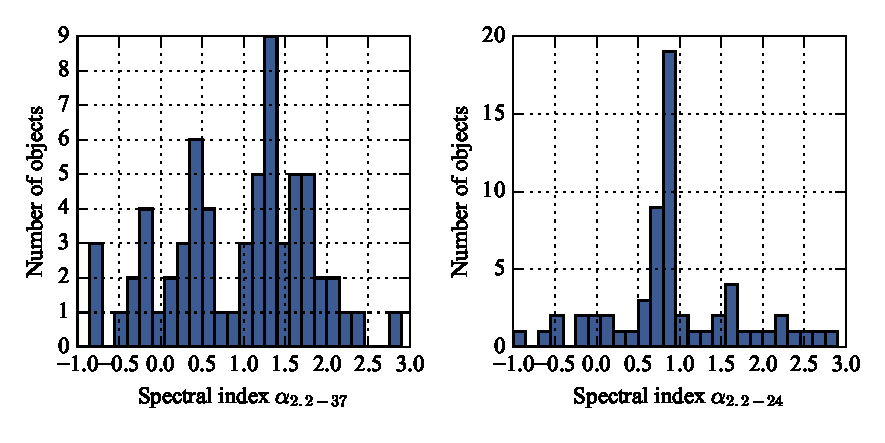
\includegraphics[width=\textwidth]{Figures/SpectralIndex.pdf}
\vspace{-1cm}
\caption[Spectral Index distribution of point sources]{Spectral Index distribution of point sources. \textit{Left}: standard determination of the spectral index, using 2MASS and \Spitzer from \SI{2}{\micron} to \SI{24}{\micron}, when data is available. \textit{Right}: Determination of the spectral index using data from 2MASS, \Spitzer and our FORCAST data up to \SI{37}{\micron}. The distribution changes significantly when you account for the longer fluxes in these clustered regions.}
\label{fig:SpectralIndex}
\end{center}
\end{figure}

The final data release also includes all of the physical parameters derived using the technique from Section~\ref{sec:SEDFitting}, as well as their uncertainties.
																							
\section{SED fitting}
\label{sec:SEDFitting}
\subsection{A custom grid of models}

SED fitting is prone to many degeneracies: usually many geometrical and physical parameters are used to construct detailed radiative transfer models, but only a handful of measurement points are available to fit, leading to a dramatically under-constrained problem. As our starting point of our investigation of the SEDs of these sources, we used the \textit{sedfitter} tool from \citep{Robitaille:2006cb}. These authors computed a large grid of tens of thousands of SED models using a radiative transfer code by \citep{Whitney:2003ke}, by varying 14 geometrical and physical parameters in the dust density grid such as the size of the disk, the accretion rates, the radius and mass of the envelope, etc. The models are then evaluated in the bands corresponding to our data, and a $\chi^2$ metric is evaluated for each model. By exploring the distribution of $\chi^2$, we noticed, as expected, the very large correlations between the parameters which is indicative of many local minimas in the grid. Hence, inferring geometrical and physical parameters from such a grid can be misleading.

We used a more modern version of the same core radiative transfer code, called Hyperion, to develop our own capability of simulating SEDs and understand the sensitivity of these parameters on the SED shape of our Class 0 and I sources. Based on our investigation, the degeneracy between viewing angle and multiple geometrical parameters is considerable. In particular, the sensitivity of the disk properties is minimal, as most of the SED properties are determined almost entirely by the envelope. In addition, parameters of the central source such as the mass, radius and temperature are irrelevant, as they are all combined into one single term, which is the central luminosity. Similarly, the luminosity created when simulating a disk accreting onto the central object can not be distinguished from a more luminous central object and a non-accreting disk. Finally, we find that there is very little difference between Ulrich envelope models and standard power-law envelopes (see for example Fig.~14 from \citet{Whitney:2013cw}), except that the latter can more directly be related to physical parameters such as the envelope mass. 

From these findings, we created a simplified grid of models by significantly reducing the number of parameters. The resulting choices are presented in Table~\ref{tab:SEDModelGrid}. Unlike most authors, who use multiple kinds of dust models for different regions of the SED (which add complexity and number of parameters), we simply use the same dust model (OH5) for both the envelope and the disk, and assume a 1:100 dust-to-gas ratio. The two main parameters that we use are the central luminosity and the envelope mass, as these are the two main physical quantities that we are trying to determine from the data. 


\renewcommand{\arraystretch}{1.5}
\setlist[itemize,1]{nolistsep,leftmargin=*,labelsep=-\mylen}
\def\labelitemi{--}
\begin{table}[!h]
\scriptsize
\caption[SED model grid]{SED model grid.}
\label{tab:SEDModelGrid}
\vspace{-0.5cm}
\begin{longtable}{lP{5cm}P{3cm}P{2cm}}
\toprule																			
Parameter	&	Description	&	Values	&	Units	\\
\midrule							
\midrule							
\multicolumn{4}{c}{Constant parameters}							\\
\midrule							
\multicolumn{4}{c}{Central source}							\\
\Mstar	&	Stellar mass	&	1	&	\si{\Msun}	\\
\Tstar	&	Stellar temperature	&	4000	&	K	\\
\midrule							
\multicolumn{4}{c}{Disk}							\\
Type	&	Flared or alpha disk	&	Flared	&		\\
\Mdisk	&	Disk mass	&	0.01	&	\si{\Msun}	\\
\Rdiskmax	&	Disk outer radius	&	100	&	\si{\au}	\\
\Rdiskmin	&	Disk inner radius	&	 sublimation radius	&	\si{\au}	\\
$\beta$	&	Flaring parameter	&	1.25	&		\\
$p$	&	Disk surface density exponent	&	-1	&		\\
$r_0$	&	Reference distance for scale height	&	\Rdiskmin	&	\si{\au}	\\
$h_0$	&	Disk scale height at $r_0$	&	0.01\Rdiskmin	&	\si{\au}	\\
$d$	&	Dust	&	OH5	&		\\
\midrule							
\multicolumn{4}{c}{Envelope}							\\
Type	&	Power-law or Ulrich	&	Power-law	&		\\
\Renvmin	&	Envelope inner radius	&	\Rdiskmin	&	\si{\au}	\\
\Renvmax	&	Envelope outer radius	&	5000	&	\si{\au}	\\
$\alpha$	&	Power	&	-1.5	&		\\
$r^\textrm{env}_0$	&	Reference radius	&	\Renvmin	&	\si{\au}	\\
$d$	&	Dust	&	OH5	&		\\
\midrule							
\multicolumn{4}{c}{Cavity}							\\
$r^\textrm{cav}_0$	&	Cavity outer radius	& 	\Renvmax	&	\si{\au}	\\
$\theta_0$	&	Opening angle at $r^\textrm{cav}_0$	&	10	&	degrees	\\
	&	Flaring exponent	&	1.5	&		\\
$\rho_0$	&	Density at $r^\textrm{cav}_0$	&	0	&	\si{\gram\per\centi\meter}	\\
$\alpha_e$	&	Density profile exponent	&	0	&		\\
\midrule							
\midrule							
\multicolumn{4}{c}{Changing parameters}							\\
\midrule							
$i$	&	Inclination angle	&	0 to 90 in 20 constant increments of cos(i)	&	degrees	\\
\Lstar	&	Central luminosity	&	$5\times 1.5^p$ for $p=-4, -3, \dots 15$ (from 0.99 to 288)	&	\si{\Lsun}	\\
\Menv	&	Envelope mass	&	$0.01\times 1.5^p$ for $p=-2, -1, \dots 20$ (from 0.004 to 22.17)	&	\si{\Msun}	\\
\Av	&	External extinction	&	$0, 1, \dots 15$	&		\\
$s$	&	Scaling	&	0.7, 0.85, 1, 1.5, 1.3	&		\\
\bottomrule					
	\end{longtable} 
\end{table}

We constructed a wrapper program that can run the Hyperion software for the parameters in this grid. Because of time and resource limitations, a moderate number of photons was chosen. The details of our modeling parameters, which will be familiar to the Hyperion user, are described in Table~\ref{tab:HyperionParams}. Note that models of more than \SI{1}{\Msun} are actually run with \num{1e6} photons for imaging, in order to obtain acceptable \SNR at short wavelengths.

\renewcommand{\arraystretch}{1.5}
\setlist[itemize,1]{nolistsep,leftmargin=*,labelsep=-\mylen}
\def\labelitemi{--}
\begin{table}[!h]
\scriptsize
\caption[Hyperion simulation parameters]{Hyperion simulation parameters.}
\label{tab:HyperionParams}
\vspace{-0.5cm}
\begin{longtable}{lP{4cm}}
\toprule																			
Number of photons (initial)	&	\num{2e5}	\\
Number of photons (imaging)	&	\num{2e5}	\\
Number of photons (raytracing sources)	&	\num{1e6}	\\
Number of photons (raytracing dust)	&	\num{1e6}	\\
Lucy max iterations	&	6	\\
Max photon interactions	&	\num{1e5}	\\
Geometrical grid parameters (radial, theta and azimuthal)	&	400, 199, 2	\\
MRW	&	True	\\
\bottomrule					
	\end{longtable} 
\end{table}

The grid is composed of 330 models which are modeled with Hyperion. For models of more than \SI{0.5}{\Msun}, we interpolate the grid in mass by increments of 20\%, which allows for a finer sampling at higher masses, but increases the number of individual models to 914. Each model is sampled at 20 inclinations, 15 values for external extinction, and five different scaling factors, for a total of $\sim 1.4$ million grid models. Each model is evaluated at all relevant observing bands, from the 2MASS bands all the way to \SI{1.3}{\milli\meter} SMA bands. Given the sparsity of the grid, and the relatively simply model used, we do not apply color correction to the fluxes, nor do we convolve the model fluxes with the band transmission function: the resulting corrections usually fall well within our approximations, and do affect significantly the outcome of the fitting.

The scaling factor is used to show the uncertainty in the distance determination \citep{Robitaille:2006cb}, but it can also be considered as a factor to sample different luminosities \citep{Furlan:2016df}. Indeed, \citet{Furlan:2016df} show that, to first order, changing luminosities by a small amount is approximately equivalent to scaling the SED in flux. In their grid, they use a scaling factor that ranges from 0.5 to 2.0, which allows them to have factors of two between their luminosity steps. We choose a more conservative approach  by actually running the grid at closer luminosity steps (factor of 1.5) and hence have a smaller scaling factor. 

The extinction parameter is used to represent extinction by material along the line of sight that is \textit{outside} of the core, commonly used for foreground material. A discussion of this parameter is proposed in the following sections.



\subsection{Fitting method}

In order to determine which model fits the data best, we adopt a metric defined by \citet{Fischer:2012dj}:

\begin{equation}
R = \frac{1}{N}\sum_i w_i|\log[\Fobs(\lambda_i)] - \log[\Fmod(\lambda_i)]|,
\end{equation}
where $i$ are the indices of the valid data points, the weights $w_i$ correspond to the inverse of the fractional uncertainty of each measurement, \Fobs and \Fmod are the observed and model fluxes respectively, and $N$ is the number of valid measurements. For our models, we set the fractional uncertainty to a minimum of 10\%, to avoid having just a few points completely over-constrain the problem.

\citet{Furlan:2016df} discuss in more detail the meaning of this metric, which differs from a standard $\chi^2$ metric such as the one used by \citet{Robitaille:2007dl}. Here $R$ represents a weighted average of the logarithmic deviations between the observations and the model. It is important to note that, although it is normalized, it does not have a statistical interpretation like the standard $\chi^2$ metric does. 

For each source, we calculate $R$ for each model in our grid. The model with the smallest value for $R$ is the best-fitting model by this metric, but given our sparse sampling and the errors of our observations, this is not necessarily the best estimate for the model which best fit the data. We can consider two extremes to this case: in the first, the best fit has a value of $R$ which is much lower than for other models. Then, it is clearly the best fit. In the second case, let's suppose that the 1000 best-fitting models lie very close to the best $R$. In this case, concluding that the model that best fits our observations (and from which will interpret physical quantities) is the one with the minimum $R$ is too strict and does not account for the uncertainties that are present in this exercise. 

In practice, all of our models fall in that second case, since our parameter grid sampling is sufficiently dense. After visual inspection we estimate there is very little significant difference between values of $R$ which are separated by $\sim 0.5$, as they all can be considered equally good fits. Hence, for a robust measure of the best-fitting model parameters, we choose the mode (the most likely value) of the parameters from models which are within $R_\textrm{min}$ and $R_\textrm{min}+0.2$. The error on the parameter estimate is then estimated using the models within $R_\textrm{min}$ and $R_\textrm{min}+0.5$, and is described in the next section.

\subsection{Overview of derived parameters}

The distribution of the best fit of the envelope mass and central luminosity is shown in Fig.~\ref{fig:MassLumHist}. Our sample covers a broad range of masses, but is naturally biased towards high luminosities given our instrumental sensitivity and cluster selection.


\begin{figure}[!h]
\begin{center}
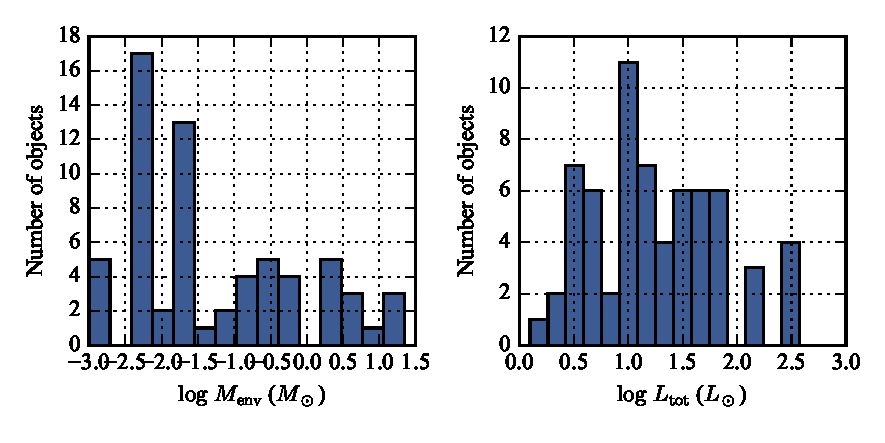
\includegraphics[width=\textwidth]{Figures/MassLumHist.pdf}
\vspace{-1cm}
\caption[Fitted envelope mass and luminosity distribution]{Fitted envelope mass and luminosity distribution.}
\label{fig:MassLumHist}
\end{center}
\end{figure}

The simple grid that we used manages to fit most of the data pretty well. The distribution of $R$ for all the isolated point sources is shown in Fig.~\ref{fig:Rdistr}. Note that targets where less data points are available, or where data points are more noisy, usually have lower $R$ than targets with a lot of available data points, even if the fits are not necessarily as good. This has also been observed by \citep{Furlan:2016df}.

\begin{figure}[!h]
\begin{center}
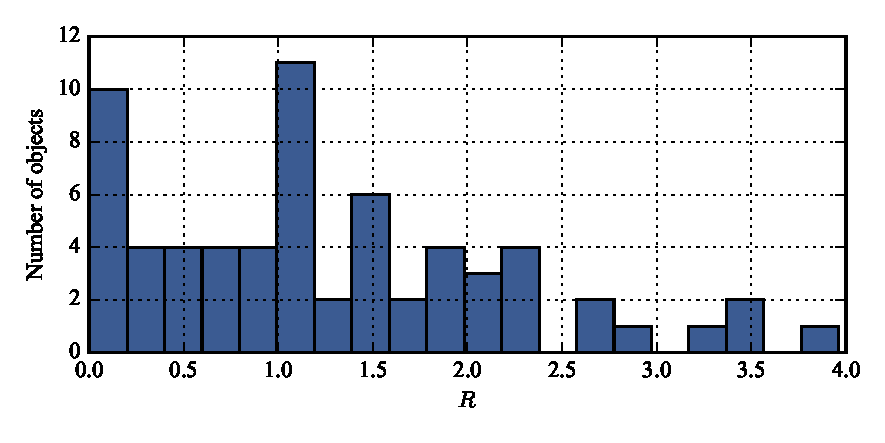
\includegraphics[width=\textwidth]{Figures/Rdistr.pdf}
\vspace{-1cm}
\caption[Distribution of $R$]{$R$ distribution across all point sources.}
\label{fig:Rdistr}
\end{center}
\end{figure}


For our sample, we can compare the fitted central luminosity, \Ltot, with the integrated luminosity from the datapoints, \Lbol (Fig.~\ref{fig:LbolVsLest}) for our entire sample of point sources. This shows relatively good agreement, although a systematic excess in fitted central luminosity can be observed, which we attribute to the widespread choice of using an external extinction coefficient. By using this external extinction as a model parameter, we artificially reduce the emission at short wavelengths, which would tend to decrease the bolometric luminosity.
\begin{figure}[!h]
\begin{center}
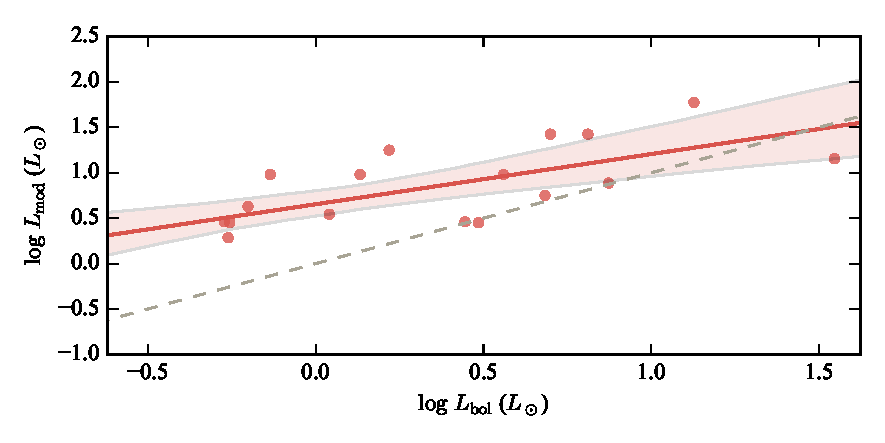
\includegraphics[width=\textwidth]{Figures/LbolVsLest.pdf}
\vspace{-1cm}
\caption[Estimated luminosity vs bolometric luminosity]{Estimated luminosity vs bolometric luminosity. The best fit line is shown in red, along with 95\% confidence intervals. The grey dashed line represents $\Ltot = \Lbol$. The excess modeled luminosity for smaller luminosities is caused by the external extinction, which absorbs a large fraction of the luminosity emitted by the central object but does not re-radiate it at longer wavelengths - this is one of the limitations of this exercise.}
\label{fig:LbolVsLest}
\end{center}
\end{figure}

The luminosity excess is more pronounced for lower masses, as the short wavelength emission represents a larger portion of the total emission from the source (Fig.~\ref{fig:LbolMinusLestVSMass}). 

\begin{figure}[!h]
\begin{center}
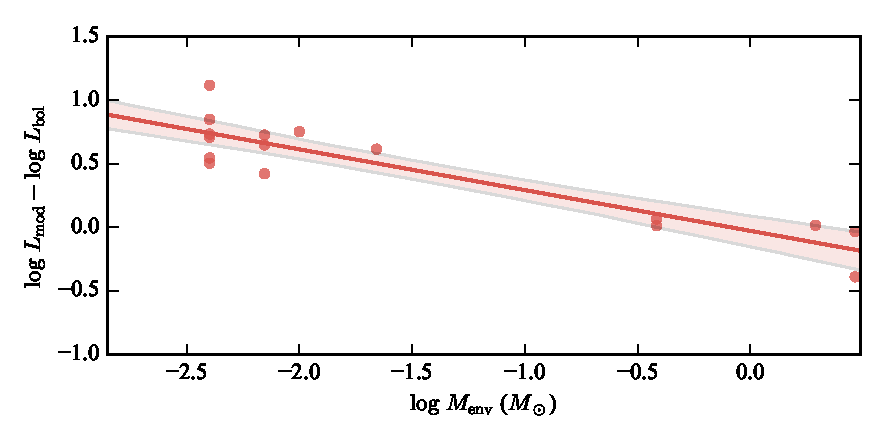
\includegraphics[width=\textwidth]{Figures/LbolMinusLestVSMass.pdf}
\vspace{-1cm}
\caption[Luminosity excess as a function of envelope mass]{Luminosity excess as a function of envelope mass.}
\label{fig:LbolMinusLestVSMass}
\end{center}
\end{figure}




We find that this is a major limitation and inconsistency to all known SED fitting methods. \citet{Furlan:2016df} fit for extinction more than we do: they allow the external extinction to go up to $\Av = 40$ for some of their sources, and use all of the 2MASS bands in their fitting. It is not consistent to assume that so much dusty material is present along the line of sight and only affect the short wavelengths, while not also being observed at longer wavelengths. Since the dust is optically thin at longer wavelengths, the far-infrared and submillimiter observations should account for this material which is obscuring the shortest wavelengths.

Our exploration with the fitting routine shows that limiting the external extinction helps by forcing more inclined geometries, where the light from the central star passes through the disk before reaching us. However, we were not able to account for the entirety of the short wavelength extinction by doing this, as the mid-infrared wavelength (IRAC and FORCAST bands) are also affected dramatically by more inclined geometries, which can compromise the fits. This could indicate a fundamental limit to our geometrical representation of YSOs.

For the clusters which do have submillimeter data points, the mass estimates are rather good, since these long-wavelengths points are constraining the mass along the line of sight very well. A summary of our fit results for Ophiuchus and NGC1333 is shown in Table~\ref{tab:FittedParameters}. Note that the luminosity that is used in this analysis is always the luminosity multiplied by the scaling factor $s$, under the assumption that the SED scales for small changes in luminosity. This scaling factor also represents a fundamental uncertainty in the distance measurement to our targets, as a distance error of 10\% would cause a luminosity estimate that would differ by 20\%.

\begin{landscape}
\begin{table}[!h]
\scriptsize
\caption[Fitted parameters]{Fitted parameters for the three clusters where long-wavelength photometry is available.}
\label{tab:FittedParameters}
\vspace{-0.5cm}
\hspace*{-1.5cm}
\begin{center}
\begin{longtable}{lcccccccccc}

\toprule																									
SOFIA Name	&	Coordinates	&	$R_{50}/R_{50,\textrm{cal}}$	&	$\alpha$	&	$R$	&	\Menv			&	\Ltot			&	$\Lbol$	&	Inc.	&	Ext.	&	$s$	\\
	&	J2000	&		&		&		&	\si{\Msun}			&	\si{\Lsun}			&	\si{\Lsun}	&	\si{\degree}	&		&		\\
\midrule																									
NGC1333.1	&	03h29m08s +31d21m57s	&	0.75	&	0.28	&	3.40	&	0.59	$\pm$	0.3796	&	5.6	$\pm$	3.12	&	8.38	&	0.0	&	12	&	0.85	\\
NGC1333.10	&	03h28m57s +31d14m15s	&	0.80	&	1.84	&	1.12	&	0.39	$\pm$	0.2364	&	5.6	$\pm$	1.69	&	4.82	&	18.7	&	14	&	0.70	\\
NGC1333.11	&	03h28m37s +31d13m30s	&	1.02	&	1.65	&	0.99	&	0.39	$\pm$	0.1571	&	7.7	$\pm$	1.37	&	7.47	&	18.7	&	12	&	0.70	\\
NGC1333.3	&	03h29m02s +31d20m21s	&	0.90	&	0.71	&	3.29	&	1.96	$\pm$	0.8200	&	3.5	$\pm$	0.80	&	8.10	&	0.0	&	14	&	0.70	\\
NGC1333.4	&	03h29m11s +31d18m31s	&	1.10	&	1.91	&	0.83	&	2.93	$\pm$	0.5045	&	2.8	$\pm$	0.42	&	3.06	&	18.7	&	14	&	1.00	\\
NGC1333.5	&	03h29m11s +31d18m20s	&	1.62	&	1.75	&	1.05	&	1.96	$\pm$	0.3884	&	2.9	$\pm$	1.00	&	2.79	&	18.7	&	9	&	1.30	\\
NGC1333.6	&	03h29m13s +31d18m14s	&	0.95	&	0.95	&	2.28	&	0.59	$\pm$	0.1589	&	4.3	$\pm$	1.72	&	1.16	&	18.7	&	14	&	1.00	\\
NGC1333.7	&	03h28m43s +31d17m35s	&	1.19	&	1.05	&	1.88	&	0.01	$\pm$	0.0014	&	9.6	$\pm$	2.16	&	1.36	&	50.8	&	0	&	0.70	\\
NGC1333.8	&	03h29m04s +31d16m04s	&	0.77	&	1.14	&	1.03	&	2.93	$\pm$	1.1268	&	14.3	$\pm$	2.24	&	35.11	&0	&	12	&	1.30	\\
NGC1333.9	&	03h28m56s +31d14m37s	&	0.80	&	2.82	&	2.63	&	2.93	$\pm$	0.5367	&	19.5	$\pm$	3.67	&	24.28	&	18.7	&	14	&	1.30	\\
Oph.1	&	16h27m10s -24d19m13s	&	0.92	&	0.27	&	0.62	&	0.017	$\pm$	0.0022	&	9.6	$\pm$	1.80	&	3.63	&	65.1	&	4	&	0.70	\\
Oph.10	&	16h27m18s -24d28m55s	&	1.26	&	0.45	&	1.89	&	0.014	$\pm$	0.0028	&	1.9	$\pm$	0.38	&	0.55	&	61.7	&	14	&	1.15	\\
Oph.13	&	16h27m30s -24d27m43s	&	--	&	-0.39	&	3.46	&	0.014	$\pm$	0.0023	&	6.5	$\pm$	1.63	&	1.49	&	65.1	&	14	&	1.30	\\
Oph.14	&	16h27m28s -24d27m21s	&	1.89	&	-0.16	&	2.35	&	0.086	$\pm$	0.0405	&	2.9	$\pm$	0.78	&	0.95	&	18.7	&	14	&	1.30	\\
Oph.15	&	16h27m29s -24d39m17s	&	1.25	&	0.01	&	1.09	&	0.014	$\pm$	0.0018	&	2.8	$\pm$	0.59	&	0.55	&	54.6	&	12	&	0.70	\\
Oph.16	&	16h26m24s -24d24m48s	&	1.80	&	-0.74	&	1.49	&	0.011	$\pm$	0.0008	&	17.7	$\pm$	4.70	&	1.66	&	74.7	&	9	&	0.70	\\
Oph.17	&	16h26m24s -24d24m39s	&	0.96	&	-0.11	&	1.00	&	0.011	$\pm$	0.0017	&	4.3	$\pm$	0.88	&	0.63	&	77.8	&	14	&	0.70	\\
Oph.18	&	16h26m17s -24d23m45s	&	1.18	&	0.57	&	1.15	&	0.02	$\pm$	0.0040	&	1.3	$\pm$	0.21	&	0.22	&	65.1	&	14	&	0.70	\\
Oph.19	&	16h26m30s -24d23m00s	&	2.51	&	0.53	&	1.15	&	0.014	$\pm$	0.0020	&	3.5	$\pm$	0.74	&	1.10	&	58.2	&	13	&	0.70	\\
Oph.2	&	16h26m44s -24d34m48s	&	0.93	&	0.83	&	2.08	&	0.014	$\pm$	0.0015	&	5.0	$\pm$	0.97	&	1.19	&	77.8	&	14	&	1.00	\\
Oph.3	&	16h27m09s -24d37m18s	&	0.99	&	0.57	&	1.54	&	0.017	$\pm$	0.0022	&	59.5	$\pm$	11.99	&	13.39	&	37.9	&	10	&	0.70	\\
Oph.5	&	16h27m07s -24d38m15s	&	1.31	&	0.35	&	1.74	&	0.014	$\pm$	0.0021	&	2.9	$\pm$	0.66	&	0.53	&	68.4	&	14	&	1.30	\\
Oph.6	&	16h27m16s -24d38m46s	&	1.29	&	2.39	&	0.83	&	0.014	$\pm$	0.0031	&	9.6	$\pm$	3.41	&	0.73	&	90.0	&	12	&	0.70	\\
Oph.7	&	16h27m28s -24d39m34s	&	0.97	&	1.35	&	1.57	&	0.032	$\pm$	0.0043	&	26.6	$\pm$	4.90	&	6.47	&	74.7	&	14	&	0.70	\\
Oph.8	&	16h27m37s -24d30m35s	&	1.02	&	0.55	&	1.06	&	0.017	$\pm$	0.0023	&	26.6	$\pm$	5.15	&	5.00	&	80.9	&	14	&	0.70	\\
Oph.9	&	16h27m22s -24d29m54s	&	--	&	0.49	&	2.08	&	0.011	$\pm$	0.0005	&	11.8	$\pm$	2.71	&	0.99	&	80.9	&	14	&	0.70	\\
\bottomrule																																															
\end{longtable}																																	
%\caption*{\textbf{Note:} The complete version of this table is made available electronically}			
\end{center}																						
\end{table}	
\end{landscape}			


\begin{figure}[!h]
\begin{center}
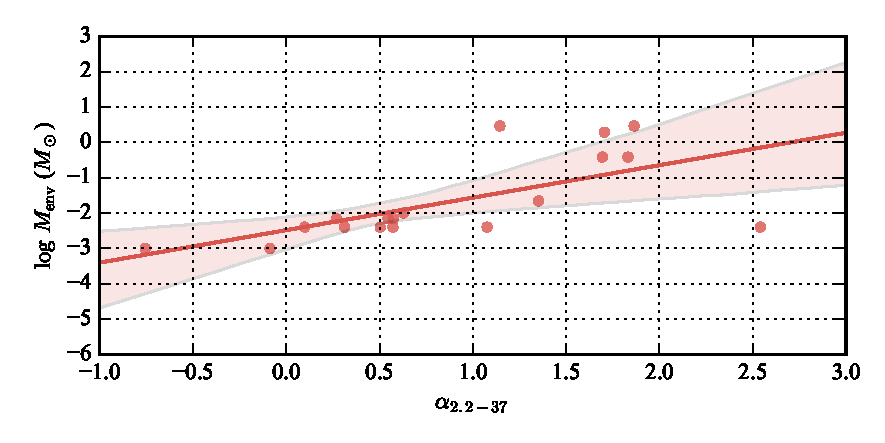
\includegraphics[width=\textwidth]{Figures/massVSalpha.pdf}
\label{fig:massVSalpha}
\vspace{-1cm}
\caption[Mass versus spectral index]{Mass versus spectral index.}
\end{center}
\end{figure}



\subsection{Estimating parameter uncertainty}

Parameter uncertainty estimation is important to quantify the confidence in a given fit, without which no meaningful conclusion can be drawn about the scientific meaning of the parameters. This estimation is also one of the most difficult aspect of this fitting process, since it really depends on the method used and the modeling strategy; it hard to compare it with the findings of different authors who might use a different strategy. 

In this work, we propose a relatively model-independent methodology to derive the uncertainty on the best fit. First, we determine the best fit for a given parameter as the mode of the parameter values from the models that fit within $[\Rmin,\Rmin+0.2]$. This statistically more robust than picking simply the model with the lower $R$, since, given our uncertainties and approximations, there is no statistically-significant difference between models that fit within that range.

Once this best fit value is determined for all parameters, the uncertainty is determined using all models that fit within $[\Rmin,\Rmin+0.5]$. We determine three quantities from these models: the standard deviation from the best fit; the median absolute deviation from the best fit; and the skewness of the distribution. All of those parameters accompany the data table which is released with this work.

We admit that the choice of the $R$ intervals are empirical, so they might not work as well for other authors. However, since the metric $R$ is not model-dependent but instead is a type of \textit{distance} between our models and our observations, we think that similar values will still lead to satisfying parameter and uncertainty estimates for other authors. One limitation could occur from the density of the grid: if the models are so sparse that there are only a handful of model within each interval used in the uncertainty estimation, this could lead to errors. 


Another important consideration is the cross-correlation between parameters. This is a phenomenon that we encountered heavily using the \textit{sedfitter} function from \citet{Robitaille:2006cb}, which attempts to fit 14-parameter models (plus extinction and scaling factor). This cross-correlation is apparent when the same observations can be fitted with models with wildly different sets of parameters, indicative of multiple local minimas in the grid.

By limiting the number of parameters in the model, we dramatically reduce this effect. However, some cross-correlations...



\subsection{Discussion}

In this exercise, several factors have been omitted for simplicity. First, the models we use have an axisymmetric geometry which is unlikely to account for realistic mass distributions in the envelope and the disk. Second, we ignore the surrounding medium and consider it devoid of emission (hence of dust). In reality, the transition to the surrounding medium is likely much closer to a continuum. Third, we assume that the only heating source is located at the center of the YSO. The heating source consists of both the light from the star, and from the accretion luminosity, which are completely which can not be distinguished from our point of view. It is important to realize that external heating can also play a role in raising the dust temperature and changing the SED signature. The impact of the interstellar heating is explored in \citet{Furlan:2016df}, who show that it can have a substantial effect on the SED - but they also not include this parameter in their grid, since it is too case-specific. The hyperion radiative transfer code that is used to model our grid can accommodate for external radiation fields as well. 

Given the relative simplicity of the model grid that we constructed, most of observations are fit well and parameters have acceptable uncertainties. This further confirms the degeneracies that exist when trying to put too much physics into very elaborate models: it is difficult to draw physical meaning just by looking at the SED. The difference in the various resolutions, sensitivity, and photometric techniques for each wavelength in the SED prevents a thorough analysis of the object, especially when located in very clustered environment when extended emission and nearby sources can contaminate the measurements. We argue that more complex models would not help in estimating the physical parameters of YSOs - but instead, this work highlights the need for higher angular resolution at wavelengths longward of \SI{37}{\um}. We note from our results that although the envelope mass appears to correlate with spectral index, the relationship is rather loose. In other words, sources with only data up to \SI{37}{\um} are likely to have poorly constrained masses, suggesting that SEDs could have the same near- to mid-IR response while having substantially different long wavelength response (REF IRAS SECTION). 

Similarly to \citet{Furlan:2016df}, we find that the distribution of inclination angles for the best fits is not uniform, which is not intuitive. There is no reason why protostars should have a selection effect in their inclination angle with respect to us. This is indicative of an artifact of the fitting process, and possibly a degeneracy between inclination angle and envelope mass (see Fig.~\ref{fig:incVSmass}), which is much more prominent when no long-wavelength data is available.



From our exploration and results, we present the following findings:
\begin{itemize}
 \item Simple models with only a few varying parameters can fit most class I and class 0 SEDs.
 \item The envelope mass and luminosity cannot be robustly predicted from looking at standard estimators such as the spectral index
 \end{itemize} 

Multi-resolution

Given that we were able to fit most SEDs with our relatively simple model grid, 

External heating; over-simple geometry; non-uniform distribution of inclination angles. Variability;

Extinction / inclination angle However, its interpretation is complicated. Extinction mostly affect the short wavelengths (after which the emission becomes optically thin, as discussed in the introduction), but it still represents a column density of material which needs to be accounted for. For example, if a model is well fit with a low envelope mass but a high extinction (suggesting that it could be a small core with a large foreground extinction), the signature of the mass that is responsible for this extinction should be visible at long wavelengths as well. Because the dust is optically thin, the far-infrared and submillimeter wavelength measurements see the integrated emission along the line of sight. When using these fluxes to fit a model, they will most often strongly influence the mass inferred from the fit. But if the model still needs more extinction to account for the short wavelength fluxes, it suggests that the geometry is not properly modeled. 



\begin{figure}[!h]
\begin{center}
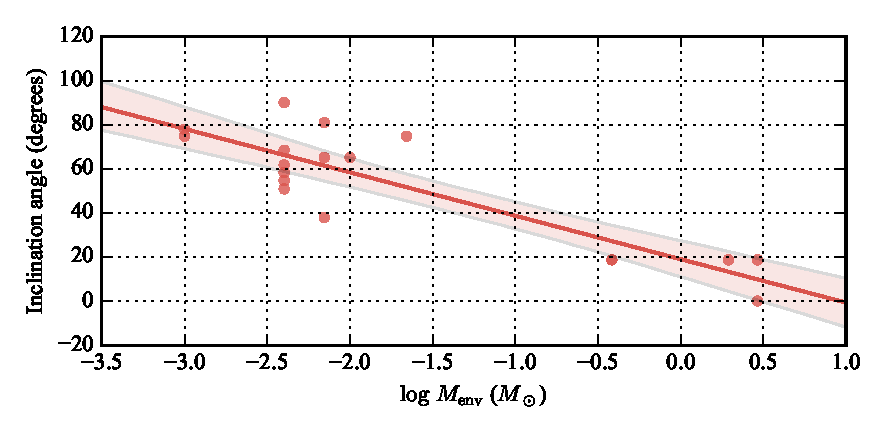
\includegraphics[width=\textwidth]{Figures/incVSmass.pdf}
\label{fig:incVSmass}
\vspace{-1cm}
\caption[Inclination versus mass]{Inclination versus mass.}
\end{center}
\end{figure}




\begin{figure}[!h]
\begin{center}
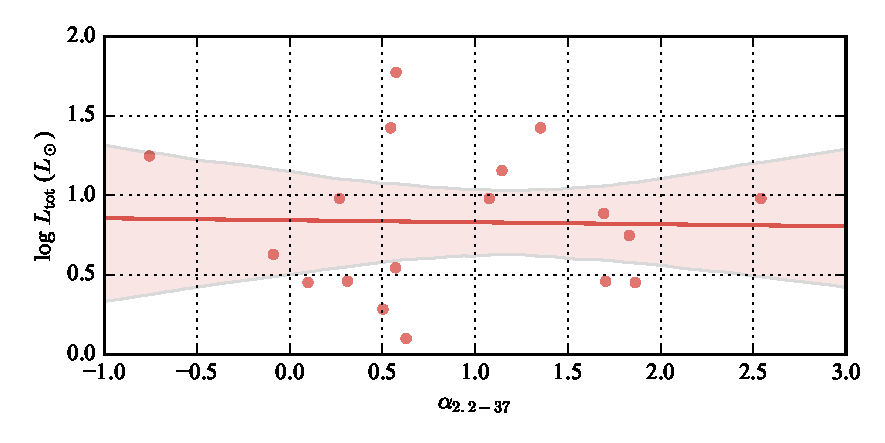
\includegraphics[width=\textwidth]{Figures/slumVSalpha.pdf}
\label{fig:slumVSalpha}
\vspace{-1cm}
\caption[Luminosity versus spectral index.]{Luminosity versus spectral index.}
\end{center}
\end{figure}



\section{Application to two clusters}

In our sample, we focus our attention on IRAS~20050+2720 and NGC~2071 that show very clustered sources which are resolved for the first time in the mid-IR with our observations with FORCAST. The fields that were observed are shown in Fig.~\ref{fig:NGC2071_IRAS20050_RGB}, superimposed with IRAC 3-color images to provide some context.

\begin{landscape}
\begin{figure*}
\begin{center}
\includegraphics[width=1.55\textwidth]{Figures/NGC2071_IRAS20050_RGB.png}
\label{fig:NGC2071_IRAS20050_RGB}
\caption[NGC2071 and IRAS20050+2720]{IRAC 3-color images of NGC2071 and IRAS20050+2720. 
%\textit{Left:} The two white squares correspond to the FORCAST fields that we observed in around the core of IRAS~20050+2720. The background RGB image is a composition of \textit{Spitzer} IRAC 8~$\um$ (red), \textit{Spitzer} IRAC 5.7 $\um$ (green) , and IRAC 3.6~$\um$ (blue). The dashed red square at the center of the image correspond to the core of the cluster, displayed in greater detail in  the picture to the right. \textit{Right:} This RGB picture shows the IRAC 1, 3, and 4 bands of the core at the center of Fig.~\ref{fig:IRAS20050_RGB}. The white contours represent the contours of the FORCAST 37~$\um$ maps, and the red circles show the FORCAST-identified point sources. An infrared nebulosity can be seen to the East of the core with physical projected size of about 0.015~pc, surrounding a cavity with slightly smaller size. The nebulosity and its cavity can be seen all the way up to 37~$\um$. The far-IR emission is mapped well onto the IRAC sources, except for SOF4, for which almost no emission can be seen at shorter wavelengths. SOF4 matches the location of the bright millimeter source MMS1 \citep{Chini:2001fa}.}
}
\end{center}
\end{figure*}
\end{landscape}




\subsection{IRAS20050+2720}

\subsubsection{Context}
IRAS~20050+2720 is part of an active site of intermediate-mass star formation in the Cygnus Rift located at \SI{700}{\pc} \citep{Wilking:1989el}, with the particularity that it doesn't seem to contain any massive stars \citep{Gunther:2012dq}. The main cluster core is associated with water and methanol masers \citep{Palla:1991up,Fontani:2010cf} and multipolar molecular outflows observed at millimeter wavelengths \citep{Bachiller:1995cy,Anglada:1998uu,Beltran:2008gu}, suggesting that the region might have experienced a recent episode of star formation in the past 0.1 Myr which contrasts with the average age of the cluster of 1 Myr \citep{Chen:1997tb,Gutermuth:2005hx}. \cite{Gutermuth:2009gca} have identified $>170$ YSOs surrounding the core and measured their continuum fluxes up to \SI{8}{\micro\meter} with IRAC. While measurements at longer wavelengths were able to provide estimates of the total luminosity of the cluster \citep[e.g. using IRAS,][\SI{388}{\Lsun}]{Molinari:1996td}, the measurements are confused in the densest region and it has not been possible to properly associate the far-IR emission with its short wavelength counterpart because of the small separation between IRAC-detected protostars. The IRAS point source was classified as a luminous class 0 protostar \citep{Bachiller:1996ja}, and its emission associated with the bright millimeter source MMS1 to the northwest of the core \citep{Chini:2001fa}. \citet{Beltran:2008gu} show strong evidence that this region has multiple generations of stars, and suggest that a group of low-mass stars first completed its main accretion phase, before setting the stage for the birth of new intermediate-mass stars at the core of this cluster.


\subsubsection{Observations and discussion}


We have observed two fields within the cluster (see Fig.~\ref{fig:IRAS20050_RGB}), including the brightest core at $20^h 07^m 06.70^s +\ang{27;28;54.5}$. Multiple sources in the core can be distinguished in the IRAC maps, but the core appears extended in \Spitzer MIPS at \SI{24}{\micro\meter}, and is identified as a single source with WISE. No high resolution far-infrared continuum data longward of \SI{24}{\micro\meter} was available for this source. To our knowledge, our observations are the only mid-IR observations available that can properly resolve the various components of the dense region. 

\begin{figure}
\begin{center}
\includegraphics[width=\textwidth]{Figures/IRAS20050_core.png}
\label{fig:IRAS20050_core}

\caption{\SI{37}{\um} observations of the IRAS~20050+2720 core, with the 5 identified objects. The blue contours are from a \SI{2.7}{\milli\meter} continuum emission observed by the OVRO array \citep{Beltran:2008gu} at levels from 10 to \SI{46}{\milli\Jy\per\beam} by increments of \SI{4}{\milli\Jy\per\beam}. The resolution of the \SI{2.7}{\milli\meter} beam is $\sim\ang{;;4.8}$, while the r.m.s noise is \SI{1.5}{\milli\Jy\per\beam}. The dashed line is the axis of a bipolar outflow identified by \citet{Bachiller:1995cy}. The beam shown at the bottom left represents the resolution of the FORCAST instrument.}
\end{center}
\end{figure}

\renewcommand{\arraystretch}{1.5}
\setlist[itemize,1]{nolistsep,leftmargin=*,labelsep=-\mylen}
\def\labelitemi{--}
\begin{table}[!h]
\scriptsize
\caption[Source fluxes in IRAS~20050+2720's dense core]{Sources fluxes in IRAS~20050+2720.}
\label{tab:IRAS20050fluxes}
\vspace{-0.5cm}
\begin{longtable}{lP{2cm}P{0.7cm}P{0.7cm}P{0.7cm}P{0.7cm}P{0.7cm}P{0.7cm}P{0.7cm}P{0.7cm}P{0.7cm}}
\toprule																			
SOFIA name	&	Coordinates	&	ks			&	i1			&	i2			&	i3			&	i4			&	F11			&	F19			&	F31			&	F37			\\
	&	J2000	&	Jy			&	Jy			&	Jy			&	Jy			&	Jy			&	Jy			&	Jy			&	Jy			&	Jy			\\
\midrule																																		
IRAS20050.1	&	20h07m06.6s +27d28m48.0s	&	0.214	$\pm$	0.021	&	0.489	$\pm$	0.049	&	0.57	$\pm$	0.057	&	0.731	$\pm$	0.073	&	0.858	$\pm$	0.086	&	0.64	$\pm$	0.07	&	1.93	$\pm$	0.20	&	4.50	$\pm$	0.35	&	6.32	$\pm$	0.59	\\
IRAS20050.2	&	20h07m06.2s +27d28m49.1s	&	0.002	$\pm$	0.002	&	0.041	$\pm$	0.004	&	0.142	$\pm$	0.014	&	0.264	$\pm$	0.026	&	0.308	$\pm$	0.031	&	0.06	$\pm$	0.06	&	1.45	$\pm$	0.19	&	9.31	$\pm$	0.72	&	11.96	$\pm$	1.19	\\
IRAS20050.3	&	20h07m06.3s +27d28m56.6s	&	0.028	$\pm$	0.003	&	0.09	$\pm$	0.009	&	0.218	$\pm$	0.022	&	0.339	$\pm$	0.034	&	0.429	$\pm$	0.043	&	0.18	$\pm$	0.06	&	2.58	$\pm$	0.27	&	12.53	$\pm$	0.94	&	19.34	$\pm$	1.41	\\
IRAS20050.4	&	20h07m05.9s +27d28m59.2s	&	0.002	$\pm$	0.002	&	0.023	$\pm$	0.003	&	0.039	$\pm$	0.004	&	0.053	$\pm$	0.008	&	0.055	$\pm$	0.008	&	0.06	$\pm$	0.05	&	0.25	$\pm$	0.20	&	8.54	$\pm$	0.80	&	12.85	$\pm$	1.25	\\
IRAS20050.5	&	20h07m06.6s +27d28m53.1s	&	0.042	$\pm$	0.004	&	0.118	$\pm$	0.012	&	0.176	$\pm$	0.018	&	0.235	$\pm$	0.024	&	0.32	$\pm$	0.032	&	0.19	$\pm$	0.05	&	1.03	$\pm$	0.21	&	2.97	$\pm$	0.33	&	5.65	$\pm$	0.65	\\
IRAS20050.6	&	20h07m02.2s +27d30m26.0s	&	0.155	$\pm$	0.016	&	0.537	$\pm$	0.054	&	0.771	$\pm$	0.077	&	1.113	$\pm$	0.111	&	1.805	$\pm$	0.181	&	1.81	$\pm$	0.13	&	2.29	$\pm$	0.17	&	1.64	$\pm$	0.14	&	1.22	$\pm$	0.38	\\
IRAS20050.7	&	20h07m07.9s +27d27m15.8s	&	0.002	$\pm$	0.002	&	0.004	$\pm$	0.004	&	0.024	$\pm$	0.002	&	0.06	$\pm$	0.006	&	0.072	$\pm$	0.007	&	0.06	$\pm$	0.05	&	0.11	$\pm$	0.06	&	1.15	$\pm$	0.14	&	2.09	$\pm$	0.31	\\				
	\end{longtable} 
\end{table}

We distinguish 5 sources which appear to share an envelope at \SI{37}{\um}. These sources are labeled in Fig.~\ref{fig:IRAS20050_core}. IRAS20050.4 is coincident with the source at the northwestern end of the region, which is name OVRO1 in \citet{Beltran:2008gu}. Two more sources are identified with these contours, to the south and east of OVRO1, but they do not appear to correlate with our SOFIA sources. The outflow axis \citep[Outflow "A",][]{Bachiller:1995cy} appears to be aligned with extended emission that is visible to the east of the 5 sources. This extended emission is visible in both IRAC and FORCAST, and could be coinciding with CO velocity maps from \citet{Beltran:2008gu} showing blueshifted gas. The emission, totalling $\sim\SI{6}{\Jy}$ at \SI{37}{\um}, appears diffuse and not connected to any particular YSO: this requires a mechanism to keep the dust emitting at these wavelengths, since no viable heating source is available to heat this material at these distances (many thousands of au from the nearest YSO).

Since the emission appears associated with the outflow, one possible scenario is that  the material was recently ejected from the central clump of YSOs by this powerful outflow. This could be material from the diffuse envelope which seem to surround the 5 sources, or material from one given YSO's gravitationally bound envelope. The gas and dust being ejected at high velocities \citep{Bachiller:1995cy}, it might not yet have time to completely thermalize with the surrounding medium (at which point it would not emit at these wavelengths). This scenario could be confirmed with high sensitivity sub-millimeter maps of the region, with a focus on dense gas tracers that would follow the mass in these regions. The existing maps from \citet{Beltran:2008gu} do not have sufficient sensitivity or resolution to properly identify the velocity field from the gas associated with this continuum emission.

Another possible explanation for this emission is that the gas and dust ejected from the cluster is heated by colliding with cold material in the surrounding medium. This could explain the bullet-like shape of the emission, and makes sense given the very high velocities from the outflow. The emission could arise from a supersonic shock layer that heats up the dust to a few hundreds of K, at which point its emission could become visible in the IRAC and SOFIA bands. 

\begin{landscape}
\begin{figure}
\begin{center}
\hspace*{-1.2in}
\includegraphics[width=1.4\textwidth]{Figures/IRAS20050.png}
\vspace{-0.5in}

\caption{The core of IRAS20050+2720 is seen in the four bands of the \textit{Spitzer} IRAS instrument, as well as with the four FORCAST bands. The increased resolution of FORCAST compared to previous instruments allows to match the long-wavelength emission with its short wavelength counterpart. The stretch in each image is adjusted for optimal readability. The white contours correspond to the FORCAST \SI{37}{\micro\meter} emission [mention the contour levels]. }
\label{fig:IRAS20050_mosaic}
\end{center}
\end{figure}
\end{landscape}

The 5 sources in the densest part of the cluster are all highly extincted based on the slopes of the emission in the 2MASS bands and the depth of the \SI{10}{\um} silicate absorption feature (Fig.~\ref{fig:IRAS20050_SEDs}. IRAS20050.1 has a flat spectrum out to \SI{37}{\um}, unlike the four other sources which are rising. IRAS20050.4 is the most steeply rising source, and is barely detected in the IRAC bands, suggesting that it is the most embedded source, which is corroborated by the fact that it is coincident with the strongest millimeter source in the region. 


\begin{figure}
\begin{center}
\hspace*{-1in}
\includegraphics[width=1.4\textwidth]{Figures/IRAS20050_SEDs.png}
\label{fig:IRAS20050_SEDs}

\caption[IRAS20050+2720 SEDs]{SEDs of the 7 sources in the two fields. }
\end{center}
\end{figure}


In testing the various scenarios of star formation, it is useful to obtain a measure of how much mass is available for the YSOs to grow after their original collapse. For this, clustered regions such as this one are an ideal laboratory since the YSOs usually appear to share an envelope. In this cluster, the typical separation between the sources are \ang{;;6}-\ang{;;8}, which correspond to projected distances of \num{3000}-\SI{5600}{\au}. This strongly indicates that the envelopes of individual YSOs are interacting with each other.


However, appropriately measuring the flux from each individual source in these clustered regions is challenging, since the sources are so close together. With an aperture of \ang{;;2.4} (3 pixel radius), we managed to put non-overlapping apertures for all the 5 sources in IRAS~20050+2720. but since the aperture correction was derived considering a "total flux" aperture to be $\sim$12 pixel radius, we are accounting for the same flux multiple times, even if the apertures are not overlapping. If we estimate the \SI{37}{\um} flux from the eastern extended emission to be totalling $\sim\SI{5}{\Jy}$, we obtain about 22\% of excess \SI{37}{\um} flux when comparing the sum of the point sources and the total emission from the cluster (see Table~\ref{tab:IRAS20050sum}). At \SI{31}{\um}, the flux excess is only about 10\%. At \SI{19}{\um} and below, the extended emission is within the noise uncertainty of the map. 

This excess flux can only partially be explained by the tails of the PSF extending well below the aperture size (see Fig.~\ref{fig:average_EE}), with 10-15\% of the total energy still existing in the annulus outward of 8~pixels (\ang{;;6}) from the aperture center. However, the contribution of a source to any given other source is only a fraction of this since it would only correspond to the amount of flux within a 3-pixel aperture. We conclude that the PSF shape is not responsible for the observed excess flux at both wavelengths.

One possible explanation would be that diffuse thermal emission occurs across the entire region. This could be caused by heating internal to the cluster (powered by the outflow, for example, like the eastern extended emission) or by a population of stochastically heated very small grains, which are not in LTE. The high outflow activity in this region could carve out multiple cavities which facilitate heating from the individual stars to extended our to larger distances within the envelopes and the shared mass reservoir. At \SI{37}{\um}, the level of diffuse emission required to account for the excess flux is about \SI{0.05}{\Jy\per\pixel}, which is the same as the average diffuse emission in the eastern region. Such an explanation would also help account for the high amount of external extinction that is needed to fit most of the SEDs in this region.

This tends to favor a scenario where protostars are fragmenting from a cloud and continue accreting material within that original envelope. The envelopes of neighboring YSOs interact, and possibly can exchange material as some YSOs become more massive (competitive accretion). 

\renewcommand{\arraystretch}{1.5}
\setlist[itemize,1]{nolistsep,leftmargin=*,labelsep=-\mylen}
\def\labelitemi{--}
\begin{table}[!h]
\scriptsize
\caption[Clustered sources in IRAS20050+2720's dense core]{Clustered sources in the densest region of IRAS20050.}
\label{tab:IRAS20050sum}
\vspace{-0.5cm}
\begin{longtable}{lP{2cm}P{2cm}P{2cm}P{2cm}}
\toprule																			
SOFIA name	&	F11	&	F19	&	F31	&	F37	\\
	&	Jy	&	Jy	&	Jy	&	Jy\\
\midrule									
IRAS20050.1	&	0.64	&	1.93	&	4.50	&	6.32	\\
IRAS20050.2	&	0.06	&	1.45	&	9.31	&	11.96	\\
IRAS20050.3	&	0.18	&	2.58	&	12.53	&	19.34	\\
IRAS20050.4	&	0.06	&	0.25	&	8.54	&	12.85	\\
IRAS20050.5	&	0.19	&	1.03	&	2.97	&	5.65	\\
\midrule									
Sum of point sources in cluster	&	1.13	&	7.24	&	37.84	&	56.11	\\
Total cluster emission	&	1.79	&	7.07	&	37.36	&	49.33	\\
Ratio	&	1.58	&	0.98	&	0.99	&	0.88	\\
\bottomrule					
	\end{longtable} 
\end{table}


%Cite also: \citep{Kumar:2006jo} if we want to talk about multiple generations of star formation.

\subsection{NGC 2071}

\subsubsection{Context}
The NGC~2071 star-forming region is one of several active areas of star formation in the northern part of L1630 giant molecular cloud which is located at a distance of \SI{422}{\pc} \citep{vanDishoeck:2011em}. NGC~2071 itself is a reflection nebula.
The NGC~2071 infrared cluster, located about 4' north of the reflection nebula, is a region of intermediate mass star formation \citep{Strom1976, Persson1981, Butner1990}. Maps of the cloud in CO and its isotopomers \citep{Buckle2010} show a large scale clump with $\sim\SI{1000}{\Msun}$ associated with the cluster. Dust continuum emission at $\lambda$=0.85 and \SI{1.3}{\milli\meter} peaks on center of the cluster extending ~1' in diameter containing ~\SI{30}{\Msun} of gas and dust \citep{Johnstone2001,Mitchell2001,Launhardt1996}. Emission from CS in the J=2-1 through J=7-6 indicate that the gas in this region is centrally condensed with a density of $sim\SI{1e6}{\raiseto{-3}\centi\meter}$ \citep{Zhou1990}. 

There are a number of near infrared surveys of the young cluster \citep[e.g.,][]{Strom1976,Lada1991,Megeath2012,Spezzi2015}. \cite{Spezzi2015} identify 52 YSOs associated with the NGC~2071 cluster, with the majority Class II sources. \cite{Flaherty2008} estimate an age of $\sim$\SI{2}{\mega\year} for the cluster, consistent with the large fraction of Class II sources (\cite{Evans2009}. The brightest far infrared emission from the cluster is associated with the IRS1 region \citep{Harvey1979,Butner1990}, which has an estimated total luminosity of \SI{520}{\Lsun}. The immediate region of IRS 1 is, in fact, home to a number of YSOs that are infrared, X-ray, and radio sources \citep{Skinner2009,C-G2012,Kempen2012}. The radio \citep{C-G2012} and H$_2$ emission line imaging indicate that IRS~1, IRS~2, IRS~3, and, perhaps, VLA~1 are YSOs with outflows. The larger scale molecular outflow associated with this region is well studied in a number of molecules \citep{Bally1982,Chernin1993,Stoji2008}.

Figure \ref{fig:n2071overview} shows the Spitzer 3.1~$\mu$m image of the IRS~1 region on the left \citep[image from Spitzer Archive:][]{Megeath2012} and the Herschel 70~$\mu$m image on the right (image from Herschel Archive: Gould Belt Project, P.I. Andr\'e). The plus marks in both panels indicate the position of the brighter YSOs: IRS~1, IRS~2, IRS~3, IRS~4, and VLA~1. The inner red circle with a diameter of \ang{;;26} indicates the extend of the saturated region in the Spitzer MIPS \SI{24}{\um} image; the outer red circle, diameter \ang{;;60}, encompasses the region with strong imaging artifacts in the MIPS \SI{24}{\um} image.
The right panel shows Herschel 70~$\mu$m image which does not resolve the emission from IRS~1, IRS~2, IRS~3, and VLA~1. The centroid of the \SI{24}{\um} and \SI{70}{\um} emission is between IRS~1 and VLA~1 indicating that several of the sources are contributing to the total observed emission. Interferometric observations show that the millimeter wavelength dust emission is dominated by envelopes associated with IRS~1 and IRS~3, with estimated masses of 8.2 and \SI{12.3}{\Msun} material, respectively \citep{Kempen2012}. The millimeter emission also reveals the presence of disks with radii $\le$\SI{100}{\au} associated with IRS~1 and IRS~3 \citep{Kempen2012}.

The luminosities and masses of the individual source, IRS~1, IRS~2, IRS~3, and VLA~1, are not known. The Spectral Energy Distributions (SEDs) shortward of 10~$\mu$m support their identification as embedded YSOS \citep{Skinner2009}. \cite{Skinner2009} gives a clear discussion of the possibilities for IRS~1 and concludes that it is likely a mid-to late B~star. \cite{Kempen2012} find luminosities of 10, 3.4, and $\le$\SI{27}{\Lsun} for IRS~1, 2, and 3, respectively, and stellar masses of $\le$\SI{1}{\Msun} for each, based on SED fitting. These masses and luminosities are not consistent with estimate of the total luminosity of the region of \SI{520}{\Lsun} \citep{Butner1990}. The far infrared images from Herschel reveal that IRS~1 alone does not totally dominate, as seen in Fig.~\ref{fig:NGC20171_saturated}; IRS~1, VLA~1, and IRS~3 likely make substantial contributions to the emission with lesser emission from IRS~2 and IRS~4.

\subsubsection{Observations and discussion}

\begin{landscape}
\begin{figure}
\begin{center}
\includegraphics[width=1.4\textwidth]{Figures/NGC2071_mosaic.png}
\label{fig:NGC2071_mosaic}

\caption{The core of NGC2071 is seen in two bands of the \textit{Spitzer} IRAC instrument ("I1" and "I4"), as well as with the four FORCAST bands. The increased resolution of FORCAST compared to previous instruments allows to match the long-wavelength emission with its short wavelength counterpart. The stretch in each image is adjusted for optimal readability. The white contours correspond to the FORCAST \SI{37}{\micro\meter} emission [mention the contour levels]. }
\end{center}
\end{figure}
\end{landscape}


\renewcommand{\arraystretch}{1.5}
\setlist[itemize,1]{nolistsep,leftmargin=*,labelsep=-\mylen}
\def\labelitemi{--}
\begin{table}[!h]
\scriptsize
\caption[Sources in NGC2071's dense core]{Sources in the densest region of NGC2071.}
\label{tab:IRAS20050sum}
\vspace{-0.5cm}
\begin{longtable}{lP{2cm}P{2cm}P{2cm}P{2cm}}
\toprule																			
SOFIA name	&	F11	&	F19	&	F31	&	F37	\\
	&	Jy	&	Jy	&	Jy	&	Jy	\\
\midrule									
NGC2071.1	&	10.07	&	72.041	&	167.93	&	234.93	\\
NGC2071.2	&	0.38	&	11.207	&	56.70	&	89.55	\\
NGC2071.3	&	0.19	&	3.027	&	19.97	&	37.56	\\
\midrule									
Sum of point sources in cluster	&	10.65	&	86.28	&	244.61	&	362.03	\\
Total cluster emission	&	13.523	&	94.16	&	280.14	&	362.99	\\
Ratio	&	1.27	&	1.09	&	1.15	&	1.00	\\
\bottomrule					
	\end{longtable} 
\end{table}



Show sum of sources compared to cluster total


\section{Conclusion and future work}

We have used SOFIA FORCAST to image 42 fields in bright, nearby stellar clusters. We derive aperture photometry in 4 bands: \SI{11.1}{\um}, \SI{19.7}{\um}, \SI{31.5}{\um}, \SI{37.1}{\um}, for a total of 90 sources. In many cases, our photometry is the only available mid- to far-IR photometry available for these sources, since archival \Spitzer observations were either saturated or confused.

In multiple cases, we complete our SOFIA photometry using \Spitzer IRAC as well as \Herschel data. When the catalogs cannot be found, we use the same photometry pipeline that we developed for SOFIA on the \Spitzer and \Herschel calibrated images.

We also proceed to SED fitting of our sources, based on a radiative transfer code called Hyperion. Using this code, we produce estimates for physical parameters of these YSOs, and carefully approximate the error in the parameter estimate.

We take a closer look at one special cluster, IRAS~20050+2720, which contains five close-by YSOs sharing what appears to be an extended envelope, favoring a competitive accretion scenario.

In our sample there were 15 cases of extended emission at \SI{37}{\um}. This spatial extension is not simple to model: with a FORCAST FWHM of $sim\ang{;;3.5}$, an object with spatial extension has a size on the order of a few thousands of \si{\au} at \SI{500}{\pc}: we haven't been able to show that the central object can heat dust grains at this distance sufficiently for them to emit thermally at \SI{37}{\um}. Hence, another heating mechanism is responsible for this emission: we suggest that the emission could be due to a population of non-LTE, very small dust grains. Answering this question will require further analysis and more study.
%\section{Introduction}
%Most stars in the Galaxy form in cluster environments of sizes 2-4 pc, often containing more than 100 young stellar objects (YSOs), with typical separations of $<$0.05~pc between stars near their centers \citep{Porras:2003kxa, Allen:2007wqa, Gutermuth:2009gca}.
%Previous studies have been effective in elucidating the young stellar content and distribution in clouds on large scales (parsec down to 0.05~pc) \citep{Evans-ARAA2012}, but young cluster cores, born in dense portions of molecular clouds, are more difficult to observe. They are obscured at optical through near-IR wavelengths. At mid-IR through far-IR wavelengths, the material surrounding YSOs and involved in the stellar birth process emits due to heating by the young stars, but the resolution to date has not been sufficient to isolate individual stars in the cores of most nearby young clusters.
%
%Space telescopes such as \textit{Spitzer} and WISE have tremendous sensitivity, which made them so scientifically productive, but it limits their utility in the densest regions of star-forming clusters because of detector saturated and imaging artifacts (See \citep{2008ApJ...672.1013P} for examples). This is particularly problematic at wavelengths of \SI{24}{\micro\meter} and beyond, where a bright cluster star can dominate a region 3-5 nominal resolution elements out from the star. In fact, it is often difficult for \textit{Spitzer} and WISE to provide good flux estimates for even the brightest YSOs in the cores of clusters.
%
%The FORCAST instrument on SOFIA provides the opportunity to study cluster cores at 10 to \SI{37}{\micro\meter} with better angular resolution than \textit{Spitzer} and WISE, without saturation even on the brightest sources. Although it is less sensitive than space-based instrument at comparable wavelengths due to the large thermal background noise at 13~km altitude, FORCAST images can lift degeneracies in assigning flux by separating sources that were previously unresolved or hidden by saturation artifacts. The mid-infrared fluxes of very clustered objects are essential contraints on their YSO's spectral energy distribution (SED) which is used to determine luminosity and evolutionary state.
%
%This paper presents the results for two clusters, IRAS~200050
%and NGC~2071, which were observed as part of a FORCAST survey program to observe bright, nearby star-forming cluster cores for which the \textit{Spitzer} and WISE archival data show extensive amounts of saturation and source confusion based on near infrared images. 
%
%Section 2 provides an overview of what is know about the two clusters. In section 3, we describe our data and reduction methods in detail, and discuss systematic of the FORCAST instrument. Section 4 presents our SOFIA images and discusses them in the context of other observations. Section 5 discusses flux measurements for cluster sources at other wavelengths and outlines our procedures for deriving improved fluxes where applicable. Section 6 presents Spectral Energy Distributions and fits for the SOIFA sources, and section 7 discusses our findings.
%
%\section{Target Clusters}
%IRAS~20050+2720 and NGC~2071 are embedded young stellar clusters with total luminosities in the cores that are characteristic of intermediate mass YSOs. The following two subsections provide overviews of each cluster and its environment.
%
%\subsection{IRAS20050+2720}
%
%IRAS~20050+2720 is part of an active site of intermediate-mass star formation in the Cygnus Rift located at 700~pc \citep{Wilking:1989el}, with the particularity that it doesn't seem to contain any massive stars \citep{Gunther:2012dq}. The main cluster core is associated with water and methanol masers \citep{Palla:1991up,Fontani:2010cf} and multipolar molecular outflows observed at millimeter wavelengths \citep{Bachiller:1995cy,Anglada:1998uu,Beltran:2008gu}, suggesting that the region might have experienced a recent episode of star formation in the past 0.1 Myr which contrasts with the average age of the cluster of 1 Myr \citep{Chen:1997tb,Gutermuth:2005hx}. \cite{Gutermuth:2009gca} have identified $>170$ YSOs surrounding the core and measured their continuum fluxes up to \SI{8}{\micro\meter} with IRAC. While measurements at longer wavelengths were able to provide estimates of the total mass of the cluster \citep[e.g. using IRAS,][388~$L_\odot$]{Molinari:1996td}, the measurements are confused in the densest region and it has not been possible to properly associate the far-IR emission with its short wavelength counterpart because of the small separation between IRAC-detected protostars. The IRAS point source was classified as a luminous class 0 protostar \citep{Bachiller:1996ja}, and its emission associated with the bright millimeter source MMS1 to the northwest of the core \citep{Chini:2001fa}. \cite{Beltran:2008gu} show strong evidence that this region has multiple generations of stars, and suggest that a group of low-mass stars first completed its main accretion phase, before setting the stage for the birth of new intermediate-mass stars at the core of this cluster.
%
%We have observed two fields within the cluster (see Fig.~\ref{fig:IRAS20050_RGB}), including the brightest core at $20^h 07^m 06.70^s +\ang{27;28;54.5}$. Multiple sources in the core can be distinguished in the IRAC maps, but the core appears extended in Spitzer MIPS at \SI{24}{\micro\meter}, and is identified as a single source with WISE. No good high resolution far-infrared continuum data longward of \SI{24}{\micro\meter} was available for this source.
%
%%Cite also: \citep{Kumar:2006jo} if we want to talk about multiple generations of star formation.
%
%\begin{figure*}
%\begin{center}
%\includegraphics[width=\textwidth]{Figures/RGB.png}
%\label{fig:RGB}
%\caption{
%%\textit{Left:} The two white squares correspond to the FORCAST fields that we observed in around the core of IRAS~20050+2720. The background RGB image is a composition of \textit{Spitzer} IRAC 8~$\um$ (red), \textit{Spitzer} IRAC 5.7 $\um$ (green) , and IRAC 3.6~$\um$ (blue). The dashed red square at the center of the image correspond to the core of the cluster, displayed in greater detail in  the picture to the right. \textit{Right:} This RGB picture shows the IRAC 1, 3, and 4 bands of the core at the center of Fig.~\ref{fig:IRAS20050_RGB}. The white contours represent the contours of the FORCAST 37~$\um$ maps, and the red circles show the FORCAST-identified point sources. An infrared nebulosity can be seen to the East of the core with physical projected size of about 0.015~pc, surrounding a cavity with slightly smaller size. The nebulosity and its cavity can be seen all the way up to 37~$\um$. The far-IR emission is mapped well onto the IRAC sources, except for SOF4, for which almost no emission can be seen at shorter wavelengths. SOF4 matches the location of the bright millimeter source MMS1 \citep{Chini:2001fa}.}
%}
%\end{center}
%\end{figure*}
%
%% \begin{figure*}
%% \begin{center}
%% \includegraphics[width=5in]{}
%% \label{fig:IRAS20050_RGB_core}
%% \caption{}
%% \end{center}
%% \end{figure*}
%
%
%[Include a discussion about de-reddening towards that region?]
%
%\subsection{NGC 2071}
%The NGC~2071 star-forming region is one of several active areas of star formation in the northern part of L1630 giant molecular cloud which is located at a distance of 390 pc \citep{A-T1982}. 
%NGC~2071 itself is a reflection nebula.
%The NGC~2071 infrared cluster, located about 4' north of the reflection nebula, is a region of intermediate mass star formation \citep{Strom1976, Persson1981, Butner1990}. Maps of the cloud in CO and its isotopomers \citep{Buckle2010} show a large scale clump with $\sim$1,000 M$_\odot$ associated with the cluster. Dust continuum emission at $\lambda$=0.85 and 1.3 mm peaks on center of the cluster extending ~1' in diameter containing ~30 M$_\odot$ of gas and dust \citep{Johnstone2001,Mitchell2001,Launhardt1996}. Emission from CS in the J=2-1 through J=7-6 indicate that the gas in this region is centrally condensed with a density of ~10$^6$ cm$^{-3}$ \citep{Zhou1990}. 
%
%There are a number of near infrared surveys of the young cluster \citep[e.g.,][]{Strom1976,Lada1991,Megeath2012,Spezzi2015}. \cite{Spezzi2015} identify 52 YSOs associated with the NGC~2071 cluster, with the majority Class II sources. \cite{Flaherty2008} estimate an age of $\sim$2 Myr for the cluster, consistent with the large fraction of Class II sources (\cite{Evans2009}. The brightest far infrared emission from the cluster is associated with the IRS1 region \citep{Harvey1979,Butner1990}, which has an estimated total luminosity of 520~L$_\odot$. The immediate region of IRS 1 is, in fact, home to a number of YSOs that are infrared, X-ray, and radio sources \citep{Skinner2009,C-G2012,Kempen2012}. The radio \citep{C-G2012} and H$_2$ emission line imaging indicate that IRS~1, IRS~2, IRS~3, and, perhaps, VLA~1 are YSOs with outflows. The larger scale molecular outflow associated with this region is well studied in a number of molecules \citep{Bally1982,Chernin1993,Stoji2008}.
%\begin{figure*}
%\begin{center}
%\includegraphics[width=\textwidth]{Figures/NGC2071_saturated_mosaic.png}
%\label{fig:n2071saturated}
%\caption{%NGC 2071 IRS~1 Region: The left panel show the Spitzer IRAC 3.1~$\um$ image. The right panel is the Herschel 70~$\um$ image. The green plus marks indicate the positions of IRS~1, IRS~2, IRS~3, and VLA~1. The inner red circle show the extend of the saturated region in the Spitzer MIPS 24~$\um$ image and the outer red circle encompasses the region strong affected by imaging artifacts. The gray circle on the lower right of the right panel is the resolution the 70~$\um$ image.
%NGC2071 seen with IRAC, MIPS and Herschel.}
%\end{center}
%\end{figure*}
%
%Figure \ref{fig:n2071overview} shows the Spitzer 3.1~$\mu$m image of the IRS~1 region on the left \citep[image from Spitzer Archive:][]{Megeath2012} and the Herschel 70~$\mu$m image on the right (image from Herschel Archive: Gould Belt Project, P.I. Andr\'e). The plus marks in both panels indicate the position of the brighter YSOs: IRS~1, IRS~2, IRS~3, IRS~4, and VLA~1. The inner red circle with a diameter of 26" indicates the extend of the saturated region in the Spitzer MIPS 24~$\mu$m image; the outer red circle, diameter 60", encompasses the region with strong imaging artifacts in the MIPS 24~$\mu$m image.
%The right panel shows Herschel 70~$\mu$m image which does not resolve the emission from IRS~1, IRS~2, IRS~3, and VLA~1. The centroid of the 24~$\mu$m and 70~$\mu$m emission is between IRS~1 and VLA~1 indicating that several of the sources are contributing to the total observed emission. Interferometric observations show that the millimeter wavelength dust emission is dominated by envelopes associated with IRS~1 and IRS~3, with estimated masses of 8.2 and 12.3~M$_\odot$ material, respectively \citep{Kempen2012}. The millimeter emission also reveals the presence of disks with radii $\le$100~AU associated with IRS~1 and IRS~3 \citep{Kempen2012}.
%
%The luminosities and masses of the individual source, IRS~1, IRS~2, IRS~3, and VLA~1, are not known. The Spectral Energy Distributions (SEDs) shortward of 10~$\mu$m support their identification as embedded YSOS \citep{Skinner2009}. \cite{Skinner2009} gives a clear discussion of the possibilities for IRS~1 and concludes that it is likely a mid-to late B~star. \cite{Kempen2012} find luminosities of 10, 3.4, and $\le$27~L$_\odot$ for IRS~1, 2, and 3, respectively, and stellar masses of $\le$1~M$_\odot$ for each, based on SED fitting. These masses and luminosities are not consistent with estimate of the total luminosity of the region of 520~L$_\odot$ \citep{Butner1990}. The far infrared images from Herschel reveal that IRS~1 alone does not totally dominate, as seen in Figure N; IRS~1, VLA~1, and IRS~3 likely make substantial contributions to the emission with lesser emission from IRS~2 and IRS~4.
%
%\section{SOFIA Observations}
%NGC 2071 and IRAS 200050+2720 were observed with the FORCAST instrument on SOFIA as part of a survey of selected nearby ($\le$1~kpc) bright star-forming clusters which show high protostellar density \citep{Gutermuth:2009gca} and are located in the northern hemisphere. The survey focussed on the clusters that contain one or more saturated or confused region in the archival \textit{Spitzer} and WISE data.
%
%\subsection{Data Acquisition}
%The IRAS 200050 and NGC~2071 observations were collected over three flights out of the 10-flight survey campaign. A summary is shown in Table~\ref{tab:obssummary}. Because the clusters are dominated by bright sources, the observations fit into small flight segments which filled gaps in the flight schedule. The source coordinate in Table~\ref{tab:obssummary} correspond to the centers of the green areas in Fig.~\ref{fig:IRAS20050_RGB} and Fig.~\ref{fig:n2071overview}. In each cluster, two fields separated by $\sim$ 3 arcminutes were observed to focus on two saturated regions. All fields were observed using the chop-and-node C2N mode from FORCAST, with 9-point dithering to reduce the flat field issues.
%
%%\capstartfalse
%%\begin{deluxetable*}{ccccccccccc}
%%\tablecaption{target list}
%%\tablenum{1}
%%\tablehead{\colhead{Cluster} & \colhead{RA} & \colhead{DEC} &  \colhead{Flight} & \colhead{Fields} & \colhead{Dist.} & \colhead{Time/Field} & \colhead{Sen{\_}11} & \colhead{Sen${\_}$19} & \colhead{Sen${\_}$31} & \colhead{Sen${\_}$37} \\
%%\colhead{} & \colhead{(deg)} & \colhead{(deg)} & \colhead{} & \colhead{}  & \colhead{(pc)} & \colhead{(s)} & \colhead{(Jy)} & \colhead{(Jy)} & \colhead{(Jy)} & \colhead{(Jy)}} 
%%\startdata
%%IRAS20050+2720 & 301.771 & 27.481 & F166, F131 & 2 & 700$^{1}$ & 253 & 0.026 & 0.039 & 0.068 & 0.127 \\
%%NGC2071 & 86.775 & 0.363 & F192 & 2 & 420$^{2}$ & 35 & 0.118 & 0.119 & 0.196 & 0.474
%%\enddata
%%\label{tab:obssummary}
%%\end{deluxetable*}
%%\capstarttrue 
%
%
%We observed the clusters in 4 bands: 11.1, 19.7, 31.5 and \SI{37.1}{\micro\meter}. The requested observation time in each band was calculated to detect YSOs with rising spectral energy distribution (SED) of same luminosity at the two distances of the clusters. We estimated integration time based on a rising-SED protostar model for $\sim 1.5\Lsun$. [HOW SHOULD I JUSTIFY THE FLUXES THAT WE SET AS OUR LIMITS?]
%
%Average observing time per field and average measured 1-sigma sensitivity levels are shown in Table~\ref{tab:obssummary} for the 4 bands. The measured background levels indicate the smallest detectable point source flux density at each wavelength, based on the noise measurements in the image itself. Bands 11.1 and \SI{37.1}{\micro\meter} were observed simultaneously using a dichroic filter, as were 19.7 and 31.5. However, in order to reach the required flux sensitivity for the \SI{37.1}{\micro\meter} band, we completed some of our observations with single-band observations at \SI{37.1}{\micro\meter}. 
%
%% \begin{longtable*}{ccccccc}
%% \hline
%% \hline
%% Cluster Name & Field & Field Coordinates & Band & Time (s) & Flight & Date \\
%% \hline
%
%% IRAS20050+2720 & 2 & 20h07m03s +27d30m38s & 11.1d & 135 & F131 & 2013-09-17 \\
%% IRAS20050+2720 & 2 & 20h07m03s +27d30m30s & 19.7d & 140 & F166 & 2014-05-02 \\
%% IRAS20050+2720 & 2 & 20h07m03s +27d30m47s & 31.5d & 160 & F166 & 2014-05-02 \\
%% IRAS20050+2720 & 2 & 20h07m04s +27d31m02s & 37.1d & 135 & F131 & 2013-09-17 \\
%% IRAS20050+2720 & 3 & 20h07m06s +27d28m12s & 11.1d & 135 & F166 & 2014-05-02 \\
%% IRAS20050+2720 & 3 & 20h07m06s +27d28m05s & 19.7d & 84 & F166 & 2014-05-02 \\
%% IRAS20050+2720 & 3 & 20h07m06s +27d28m13s & 31.5d & 96 & F166 & 2014-05-02 \\
%% IRAS20050+2720 & 3 & 20h07m06s +27d28m06s & 37.1d & 126 & F166 & 2014-05-02 \\
%% \hline
%
%% NGC2071 & 1 & 05h47m07s +00d17m49s & 11.1d & 18 & F192 & 2015-02-05 \\
%% NGC2071 & 1 & 05h47m07s +00d18m02s & 19.7d & 11 & F192 & 2015-02-05 \\
%% NGC2071 & 1 & 05h47m06s +00d17m55s & 31.5d & 11 & F192 & 2015-02-05 \\
%% NGC2071 & 1 & 05h47m07s +00d18m03s & 37.1d & 21 & F192 & 2015-02-05 \\
%% NGC2071 & 2 & 05h47m07s +00d21m30s & 11.1d & 18 & F192 & 2015-02-05 \\
%% NGC2071 & 2 & 05h47m07s +00d21m31s & 19.7d & 18 & F192 & 2015-02-05 \\
%% NGC2071 & 2 & 05h47m07s +00d21m34s & 31.5d & 24 & F192 & 2015-02-05 \\
%% NGC2071 & 2 & 05h47m07s +00d21m34s & 37.1d & 21 & F192 & 2015-02-05 \\
%
%% \caption{List of observations}
%% \end{longtable*}
%
%%Make sure to mention the distances picked and the references for it, as well as the cluster's age estimate
%%Need to find references to cite for details about each region
%\subsection{Data reduction}
%The data are processed through various versions of the online pipeline to yield Level 2 data products available on the archive \citep{Herter:2013by}. We apply our own reduction procedure and photometry pipeline on those products to derive final images, source positions, fluxes and sensitivities. The software utilizes the Python \textit{astropy} package \citep{2013A&A...558A..33A} and its associated modules \textit{photutils} and \textit{APLpy}. 
%
%\subsubsection{Pre-treatment}
%Some manual treatment of each image is necessary before it can be analyzed by our software, which follows this procedure: a) visually aligning the WCS coordinate system, often 10-20" off, using point sources and archival data from other wavelengths and facilities such as IRAC \SI{8}{\micro\meter}; b) cropping the images to clean off the nodded fields, and c) identify the coordinates of each source, both point-like and extended.
%
%After these manual steps, the Level 2 images are multiplied by the calibration factor provided by the online pipeline, which converts them to Jy/pixel. We do not proceed to any systematic color correction, but the effects on the fluxes are very small \citep{Herter:2013by}.
%\begin{comment}
%\begin{enumerate}
%\item Adjust WCS coordinates: use images at other wavelengths (2MASS, IRAC, MIPS, WISE) to re-align the (RA, DEC) position of the field. We estimate that this process is good to within one SOFIA pixel (0.768") for the fields where one or more point sources can be identified. Extended fields are less trustworthy, since matching the extended emission to other wavelengths is harder. The rotation of the field produced by the SOFIA pipeline is correct for all of our data. 
%\item Crop each image, remove chopped fields, remove artifacts.
%\item Identify and categorize sources: isolated point sources, clustered point sources, and extended sources. For extended sources, a circular or elliptical aperture is used to try to encompass the entirety of the emission.
%\item Manually identify a location in the field that corresponds to a representative background.
%\end{enumerate}
%\end{comment}
%\subsubsection{Source flux extraction and calibration}
%\begin{comment}
%We feed the adjusted FITS and associated metadata files to a photometry pipeline. The pipeline first processes all the calibrator stars that are observed during each flight, with each filter setting, and derives a new aperture correction factor for each image, based on an aperture of 4 pixels radius (3.072") and an aperture of 12 pixels radius. We consider that the latter aperture contains all the flux from a given point source.
%
%We distinguish between 3 types of sources after manual identification: \textit{isolated}, which are point sources with no nearby objects; \textit{clustered}, which are point sources with nearby objects; and \textit{extended}, which are not consistent with being point sources. [THIS PARAGRAPH MAY GO AWAY IF WE DON'T WANT TO TALK ABOUT GENERALITIES ABOUT THE PIPELINE]
%
%
%For point sources, we use our standard aperture of 4 pixels at all wavelengths. We consider an annulus surrounding the source extending from 12 to 20 pixels radius (24 to 40 for clustered sources): the local background is determined from the mode of the pixels in the annulus, while the sensitivity is calculated by measuring the standard deviation of 4-pixel apertures within that annulus [Cite Taro's paper and the Herschel photometry paper that Tracy gave us]. We apply the aperture correction derived from the calibrator observations taking during that flight.
%
%For extended sources, an elliptical aperture is determined manually from the \SI{37}{\micro\meter} images. The local background is determined from the mode of an elliptical annulus, with an inner boundary at the elliptical aperture and an outer boundary corresponding to an ellipse 20\% larger. The sensitivity quoted is the point source sensitivity, and is determined following the same method as for point sources, using the standard deviation of apertures spread across the elliptical annulus. [NO NEED TO MENTION THIS SINCE WE MIGHT NOT TREAT EXTENDED SOURCES]
%
%The photometry from sources that were observed in different flights is then combined to increase the signal-to-noise ratio. This combination takes into account the sensitivity of each source by appropriately weighing each image.
%
%Although we can compute source sensitivities based on the local noise, and we use the calibrators each flight to determine the aperture correction, observations with SOFIA have additional noise from the water vapor overburden and air mass, as well as from the flat field variations. These noise contributions usually amount to much higher than the sensitivities estimated from the local background, and we follow the recommendation from \citep{Herter:2012hv} to adopt a 20\% uncertainty for our flux estimates. 
%
%\end{comment}
%
%\subsection{Photometry at other wavelengths}
%
%\subsection{Instrumental Characterization}
%[THIS WHOLE DISCUSSION MIGHT FIT BETTER IN THE PAPER ABOUT THE WHOLE SURVEY, RATHER THAN THIS PAPER WHICH IS JUST ABOUT TWO CLUSTERS...]
%The three flights discussed here were part of the total of 10 data flights for the entire survey. The larger context of the entire survey allowed us to follow the evolution of the instrument properties throughout the two years of science observations. We discuss three metrics: the evolution of the aperture correction factor, the evolution of the instrument's residuals, and the evolution of the PSF size, through half width at half max of the encircled energy distribution, that we call $\Rfifty$. This is done in an attempt to assess the uncertainties in our flux determination, and our confidence in determining that sources are point-like or extended. %This study is based  on the large number of calibrator observations during our 10 science flights.
%
%\subsubsection{PSF size}
%
%Fig~\ref{fig:average_EE} shows the average of the normalized encircled energy distribution of the PSF, measured on all the calibrators of our sample. Each curve represents one of the five different combinations of bandpass filter and dichroic setting that we use for our observations: \SI{11.1}{\micro\meter}, \SI{19.7}{\micro\meter}, \SI{31.5}{\micro\meter}, \SI{37.1}{\micro\meter} with dichroic and \SI{37.1}{\micro\meter} without a dichroic (open). 
%
%As expected, the PSF at \SI{37.1}{\micro\meter} is larger than the PSFs at shorter wavelengths, but less that the traditional diffraction limit rule. This indicates that additional PSF smearing is occurring at short wavelengths, likely due to plane jitter and pointing errors. This was predicted and mentioned in the SOFIA Observer's Handbook. Throughout all the flights, the largest 1-sigma error occurs for the \SI{37}{\micro\meter} observations at about XX\%. CONCLUDE ON OUR ABILITY TO DETERMINE WHETHER A SOURCE IS EXTENDED OR NOT.
%
%To look at the behavior of the PSF in more detail, we can use the half width at half maximum of the encircled energy distribution, $\Rfifty$ as a proxy for PSF size. The variation of this quantity for the various flights, bandpass/dichroic setting, and calibrators used is showed in Fig~\ref{fig:Rfifty_dist}. This shows the flight-to-flight differences and, for some calibrators, the in-flight variability. We find that the latter is usually NN\% or less, except for the SOFIA flight on 05-02-2014, for which the spread is quite considerable. The variation from flight to flight is larger than the variation within a given flight, which indicates variability in the observing conditions, systematics, or thermal radiation environment of the observatory between different flights. Hence, we conclude that the extension of a source can be best determined by comparing $\Rfifty$ for that source with $\Rfifty$ for the corresponding calibrator measurement for that flight and dichroic setting, to within NN\%, 1-sigma confidence.
%\begin{figure}
%\begin{center}
%
%\includegraphics[width=0.45\textwidth]{Figures/average.png}
%\label{fig:average_EE}
%\caption{PSF size distribution}
%\end{center}
%\end{figure}
%
%\begin{figure}
%\begin{center}
%
%\includegraphics[width=0.45\textwidth]{Figures/fwhs.png}
%\label{fig:Rfifty_dist}
%
%\caption{PSF size distribution}
%\end{center}
%\end{figure}
%
%\subsubsection{Aperture correction}
%In Fig~\ref{fig:response}, we plot the aperture correction factor that we compute from the ratio of the flux measured within an aperture of 4 pixels, divided by the flux measured in an aperture of 12 pixel radius, which we consider to be encompassing the total flux in the source. Not surprisingly, this graph follows very closely the plot of $\Rfifty$ shown in Fig~\ref{fig:Rfifty_dist}, showing the close link between the aperture correction factor and the shape of the calibrator's PSF. For the aperture correction variability, we adopt a XX, 1-sigma uncertainty value on the flux estimate.
%
%
%
%\subsubsection{Instrument response}
%To further study the variability of the observing, we can look at the detector response and the aperture correction evolution after applying the calibration factor. In the ideal conditions, the calibration factor always leads to the same flux measurement of the calibrator source, within the pipeline's systematic errors and residual noise. The detector response is measured here by simply applying aperture photometry on the calibrators to measure their fluxes, using the same local background subtraction as the one described in the previous sections. Calibrator stars are good ways to correct for telescope and atmospheric variability, as their far-infrared fluxes are not expected to vary significantly over any relevant timescale. %We adopt a value of XX, 1-sigma value for the response variability, effectively representing the uncertainties in the observatory and the atmosphere.
%In Fig~\ref{fig:response}, we plot all the measured fluxes of the calibrators. The flux variability from flight to flight for a given calibrator is small (typically [CALCULATE THIS]), and the variability within the same flight is even smaller [QUANTIFY]. We adopt a XX, 1-sigma uncertainty value for the absolute flux measurement. This is the residual uncertainty after applying the systematic correction produced by the SOFIA FORCAST online pipeline.
%
%
%
%\begin{figure}
%\begin{center}
%
%\includegraphics[width=0.45\textwidth]{Figures/Phot_val.png}
%\label{fig:response}
%\caption{Instrumental response and aperture correction}
%
%\end{center}
%\end{figure}
%
%\begin{figure}
%\begin{center}
%\includegraphics[width=0.45\textwidth]{Figures/Aper_corr.png}
%\label{fig:aper_corr}
%
%\caption{Instrumental response and aperture correction}
%\end{center}
%\end{figure}
%
%%WHAT IS THE BOTTOM LINE FROM THIS DISCUSSION? IS A FLUX MEASUUREMENT LIMITED BY VARIATIONS IN THE PSF IF IT IS BRIGHT? SOMETHING ELSE? IT SEEMS LIKE THE CONCLUSION FROM THIS SECTION SHOULD BE A STATEMENT ABOUT THE SYSTEMATIC ERRORS ON ANY QUOTED FLUX MEASUREMENT AND A STATEMENT ABOUT LIMITATIONS ON KNOWING WHETHER A SOURCE IS EXTENDED RELATIVE TO A POINT SOURCE.
%\section{Observational results}
%\subsection{IRAS 200050}
%
%SOFIA photometry results, IRAC photometry issues and results; looking at the sources that are fit by guthermuth, we find a 10\% agreement between our photometry results and theirs.
%
%\subsubsection{Photometry results and maps}
%
%\subsubsection{SEDs}
%
%
%\subsubsection{Upper limits on other sources in the field}
%
%
%\begin{figure}
%\begin{center}
%\includegraphics[width=1\textwidth]{Figures/IRAS20050_SEDs.png}
%\label{fig:IRAS20050_SEDs}
%\caption{}
%\end{center}
%\end{figure}
%
%
%
%
%\subsection{NGC2071}
%
%
%\subsubsection{Photometry results and maps}
%
%\begin{figure}
%\begin{center}
%\includegraphics[width=1\textwidth]{Figures/NGC2071_mosaic.png}
%\label{fig:NGC2071_mosaic}
%\caption{The core of IRAS20050+2720 is seen in the four bands of the \textit{Spitzer} IRAS instrument, as well as with the four FORCAST bands. The increased resolution of FORCAST compared to previous instruments allows to match the long-wavelength emission with its short wavelength counterpart. The stretch in each image is adjusted for optimal readability. The white contours correspond to the FORCAST \SI{37}{\micro\meter} emission [mention the contour levels]. The red circles indicate the location of the five FORCAST point sources in the core.}
%\end{center}
%\end{figure}
%
%\begin{figure}
%\begin{center}
%\includegraphics[width=1\textwidth]{Figures/NGC2071_SEDs.png}
%\label{fig:NGC2071_SEDs}
%\caption{}
%\end{center}
%\end{figure}
%
%\subsubsection{SEDs}
%
%\subsubsection{Upper limits on other sources in the field}
%
%
%\subsection{Summary}
%
%Put here the table of photometry + flags
%
%
%
%\section{SED and dust modeling}
%
%YE05 assumed the dust opacities of Ossenkopf \& Henning
%(1994) appropriate for thin ice mantles after 105 year of coagulation at a gas density of 106 cm-3 (OH5 dust), which several recent studies have shown to be appropriate for cold, dense cores (e.g., Evans et al. 2001; Shirley et al. 2002; Young et al. 2003; Shirley et al. 2005) [LOOK AT REST OF DISCUSSION IN DUNHAM et al. 2010]
%
%\subsection{Radiative transfer models}
%
%We use radiative transfer models to fit the SEDs we observe and extract physical parameters. We explored the tool by \cite{Robitaille:2006cb} as a starting point for this process. While the tool provides results that fit the data well, the large number of parameters makes it difficult to draw meaningful conclusions on the real physics behind the observations. We have observed a large amount of cross-correlations between the model parameters, as well as many local minimas in the $\chi^2$ minimization scheme that is used.
%
%In an effort to understand the dependence of the observations with the physical parameters used in the models, we use the HYPERION radiative transfer code \citep{Robitaille:2011fc} and create our own grid of models by varying a small amount of meaningful parameters. HYPERION is a very versatile code with lots of options for various geometries, but we simplify the problem to its most essential components: a circularly symmetric disk with a power-law envelope.
%
%We explore the various geometries and parameters that are available in the code, and come to following conclusions:
%\begin{enumerate}
%\item Modeling accretion through an $\alpha$-disk instead of a flared disk is equivalent to increasing the central luminosity by an appropriate amount. Hence, we use only standard flared disks and quote a total central luminosity
%\item It is good enough to only vary the total luminosity of the central object, instead of varying its mass, radius and temperature
%\item Models are very insensitive to disk mass, when the envelope's mass is larger
%\item The model is sensitive to the envelope's mass distribution within a given radius, but not sensitive to the envelope's inner or outer radius
%\item The outer radius of the disk has no effect on the models
%\item The inner radius of the envelope 
%\end{enumerate}
%
%Based on our exploration of HYPERION, we proceed with the following simulation set up. We use a density structure composed of a standard flared disk of \SI{e-3}{\Msun} that extends from the dust sublimation radius out to 50~AU. The scale height at the dust sublimation radius is set to be 10\% of that radius. The disk's flaring power is a constant set to $\beta=1.1$. 
%
%We add an envelope with a central cavity. The envelope extends from 30~AU out to a variable radius, and has a variable mass and power law exponent. The inner cavity has a constant 25 degree opening angle. Setting this latter parameter has some effect that is correlated with the viewing angle.
%
%All elements in our model are using the same dust model by \cite{Draine:2003di}. We have experimented with various other types of dust models, notably with the OH5 dust [REFERENCE], as it was suggested in [CITE TRACY]. We found that the fits with the OH5 dust were much worse. In most cases, it was particularly difficult to fit the \SI{10}{\micro\meter} silicate absorption feature. 
%
%We use a variable foreground extinction also with the same dust model, as we anticipate that most of the extinction along the line of sight will occur in the cluster itself. We chose to not use any ambient medium, as they complicated the interpretation of the results.
%
%We run our simulations using $10^5$ photons, and spherical grids with 199 radial cells, 49 meridional cells, and 1 single azimuthal cell. We have tested these various parameters and sought an optimum of fast computing times and low statistical noise. With this, the calculated uncertainties are a few percent at long wavelengths and can be on the order of 10 to 15 percent at short wavelengths. This is acceptable since the short wavelength range is largely used in the fit to determine the overall external extinction magnitude. At the wavelenghts relevant for the IRAC fluxes, the uncertainties due to the simulation are on the order of 5\% - less than our estimated measurement error. With these parameters, a typical model takes about 5-10 minutes to run on a standard desktop computer. Our wrapper software allows us to run multiple different grids in a row and merge them into one single entity that we can feed to a minimization routine.
%
%In order to fit the data, we use the $\chi^2$ method described in \cite{Robitaille:2007dl}, with the exception of the overall optimal scaling step. We calculate the $\chi^2$ for our targets with all calculated models, inclinations, and a range of values of foreground extinction magnitudes.
%
%
%%Table of set parameters]
%
%%variable parameters: envelope mass, envelope density power law, source luminosity, inclination, extinction
%
%
%
%
%%This section discusses how we set up a grid of models to fit, and why we moved away from Robitaille's sedfitter. Maybe show some results from the Robitaille's fits?
%
%\subsection{Extracting physical parameters from the fits}
%This section discusses the results from the fits: best fits, parameter estimation and variation about the best fits, color-color diagrams, etc.
%\begin{itemize}
%\item \citep{Shirley:2000gh}: typical masses of protostars are a few tenths to \SI{2}{\Msun}. 
%
%\end{itemize}
%
%
%\section{Discussion}
%
%\section{Conclusion}
%blabla
 
%% Chapter 5

\chapter[Conclusion]{\setstretch{1}Conclusion} % Main chapter title


%\epigraph{\setstretch{1}\small\itshape Ever tried. Ever failed. No matter. \\ Try again. Fail again. Fail better.}{S. Beckett, \textit{Worstward Ho!}}


%----------------------------------------------------------------------------------------
%	THESIS CONTENT - APPENDICES
%----------------------------------------------------------------------------------------

\appendix % Cue to tell LaTeX that the following "chapters" are Appendices

% Include the appendices of the thesis as separate files from the Appendices folder
% Uncomment the lines as you write the Appendices

%% Appendix A

\chapter{Appendix Title Here} % Main appendix title

\label{AppendixA} % For referencing this appendix elsewhere, use \ref{AppendixA}

\section{Deriving the Interferogram Equation in a Double Fourier System}
\label{ap:interfero}
The interferogram from a double-Fourier system is different from the interferogram
for an FTS in several ways that derive from the fact
that the double-Fourier system starts with two independent input beams viewing the same astronomical target. For this derivation,
we will follow the convention in the FTS literature and consider the propagation of a single plane wave (radiation from a point source at infinity) at wavenumber $\s\equiv{1/\lambda}$ through the system.

Figure 2 in the main text shows the setup for a typical double-Fourier system with the K-mirror on one
arm to keep the sky images at the same rotation on the two paths, and the delay line
in the other arm to allow adjustment of the relative path lengths between path 1 and 2.
The plane wave travels a distance $x_1$ on path 1 from an entrance aperture an arbitrary distance
above the siderostat to the beam combiner: $a_1(\s) e^{-2\pi i \s x_1+\phi}$,
where $a_1$ is the amplitude of the electric field and $\phi$ corresponds to an arbitrary phase offset. For convenience of notation, in the following derivation we drop the amplitudes' dependence on wavenumber by writing $a_1$ instead of $a_1(\s)$.

The wave also undergoes phase shifts caused by reflections and partial reflections along
the path. A full reflection for light traveling in air or a vacuum causes a 180~$\deg$ phase shift;
a 50\% reflection at the beam splitter/combiner causes a 90~$\deg$ phase shift between reflected and transmitted beam \citep{2000plbs.conf.....L}. Since the instrument
measures the combined light at the detectors, what matters is the difference in the
numbers of reflections along path 1 and 2. In the case of the particular BETTII implementation, path 1 contains one more reflection than path 2.

The electrical fields arriving at the ``+" and ``-" detectors are then:
\begin{eqnarray}
A_- &=& a_1 e^{-2\pi i \s x_1+ i \pi + i\pi /2+\phi} + a_2 e^{-2\pi i \s x_2 +\phi },\\
A_+ &=& a_1 e^{-2\pi i \s x_1 + i \pi +\phi} + a_2 e^{-2\pi i \s x_2 + i\pi /2 +\phi},
\end{eqnarray}
where the $\pi$ phase shift on path 1 occurs because there is one extra reflection compared to path 2 (see Fig.~\ref{fig:optics}), and $\phi$ corresponds to an arbitrary phase offset. The detectors are power detectors so defining the intensity $ I = A^* A$:
\begin{eqnarray}
I_- &=& a_1^2 + a_2^2 + a_1 a_2 \left(e^{-2\pi i \s (x_1 - x_2) + 3i\pi /2} + e^{2\pi i \s (x_1 - x_2) - 3i \pi/ 2}\right),\\
I_+ &=& a_1^2 + a_2^2 + a_1 a_2 \left(e^{-2\pi i \s (x_1 - x_2)  + i\pi /2} + e^{2\pi i \s (x_1 - x_2) -  i \pi/ 2}\right).
\end{eqnarray}
Defining $x \equiv x_1 - x_2$ and expanding the complex exponentials, the equations can be simplified to:
\begin{eqnarray}
I_- &=& (a_1^2 + a_2^2 ) \left( 1 - {2 a_1 a_2 \over a_1^2 + a_2^2} \sin( 2 \pi \s x) \right),\\
I_+ &=& (a_1^2 + a_2^2 )\left ( 1 + {2 a_1 a_2 \over a_1^2 + a_2^2} \sin( 2 \pi \s x) \right),
\end{eqnarray}
where $x$ is now the difference in the physical length between the two light paths.
For the case of equal wave amplitudes on path 1 and 2 ($a_1=a_2=a$):
\begin{equation}
I_\pm = 2 a^2 ( 1 \pm \sin( 2 \pi \s x) ).
\end{equation}
The generalization of this equation to a source distribution on the sky requires the recognition that $a_1$ and $a_2$
are complex values such that $|a_1|^2(\s)$ and $|a_2|^2(\s)$ are
power from the source at wavenumber $\s$, while $a_1 a_2^*$ is the correlated power seen through the two apertures which is
the source spatial visibility, $\gamma(\baseline,\s)$, and is in general a complex valued function. $\gamma(\baseline,\s)$, which is a function of
the baseline vector $\baseline$ connecting the two light collectors, and $\s$, is the Fourier transform of the
source emission distribution on the sky.
For the general case, the previous equations become:
\begin{eqnarray}
I_- & = & |a_1|^2 + |a_2|^2 + \gamma(\baseline,\s) e^{-2\pi i \s (x_1 - x_2) + 3i\pi /2} + \gamma^*(\baseline,\s) e^{2\pi i \s (x_1 - x_2) - i 3\pi/ 2},\\
I_+ & = & |a_1|^2 + |a_2|^2 + \gamma(\baseline,\s) e^{-2\pi i \s (x_1 - x_2) + i\pi /2} +  \gamma^*(\baseline,\s) e^{2\pi i \s (x_1 - x_2) -i  \pi/ 2}.
\end{eqnarray}
The same simplification as before can be done except that $\gamma(\baseline,\s)$ is a complex-valued function. If we define the normalized spatial
visibility as
\begin{equation}
\Vb(\s) = {2\gamma(\baseline,\s)\over a_1^2 + a_2^2},
\end{equation}
then the equation for $I_\pm$ becomes:
\begin{eqnarray}
I_\pm & = & ( |a_1|^2 + |a_2|^2 ) \left[ 1 \pm (\real\left(\Vb(\s)\right) \sin(2 \pi \s x) - \imag\left(\Vb(\s)\right) \cos(2 \pi \s x))\right],\\
I_\pm & = & ( |a_1|^2 + |a_2|^2 ) \left[ 1 \pm \real\left( i \Vb(\s) e^{-2 \pi i \s x}\right)\right],
\end{eqnarray}
where $\real(f)$ is the real component of $f$ and $\imag(f)$ is the imaginary component.

The same style of derivation can be done with for a realistic instrument with a complex transfer function.  If
we characterize the spectral transmission function as $t_1(\s) = |t_1(\s)| e^{i\Phi_1(\s)} $ along path 1, and
$t_2(\s) = |t_2(\s)| e^{i\Phi_2(\s)} $ on path 2, then the amplitude mismatch of the spectral transmission function in each path reduces the power in the interferogram and
the phase differences introduce a phase factor $\Phi_{i} = \Phi_1 - \Phi_2$ into the exponential term.
As a result, the source visibility in the previous equations is multiplied by a normalized, instrumental visibility loss term, $\Vi = |\Vi(\s)|e^{i\Phi_i(\s)}$:
\begin{equation}
I_\pm = ( |t_1|^2 |a_1|^2 + |t_2|^2 |a_2|^2 ) \left[ 1 \pm \real( i \Vb(\s)\V_i(\s) e^{-2 \pi i \s x})\right].
\end{equation}
%where $\Vb(\s)$ now also includes the normalizations does to the instrument transfer function.


\section{Spectral noise in presence of gaussian phase noise}
\label{ap:phasenoise}

Suppose that the signal is a line of power density $2\S$ centered on bin number $k$ corresponding to wavenumber $\s_k$. In the complex interferogram, the line has a power density $\S$ in bin $k$ and $-\S$ at $-k$, and zero everywhere else. To simplify the analysis, let's focus on the positive frequencies, which only contain half the noise. The interferogram at delay $\xn = n\Dx$ is $\Ikxn =\S\dsig e^{-2i\pi \s_k\xn}$. Through a simple DFT, the value of the line in the spectrum in ideal conditions is:
\begin{equation}
\Dx\DFT(\Ikxn)[k'] = \Dx\sum_{n=-N/2}^{N/2-1}\S\dsig e^{-2i\pi \s_k\xn }e^{2i\pi n k'/N} = \Dx\sum_{n=-N/2}^{N/2-1}\S\dsig e^{-2i\pi (k-k')n/N },
\end{equation}
which is equal to $\Dx N\S\dsig = \S$ for $k=k'$ and zero everywhere else.
Note that we have $\s_k\xn = k\dsig n\Dx = kn/N$. and $\dsig = (N\Dx)^{-1}$. The phase noise degrades the effective power of the line, so it is now $\S e^{-\varPhir/2}$ \citep{Richards:2003bp}. The noisy interferogram is $\Ikxn =\S\dsig e^{-2i\pi kn/N}e^{i\Phir\pxn}$.

Designating the operator $\langle \rangle $ as the ensemble average, the noise $\varspec$ in the interferogram is the variance of the DFT:
\begin{eqnarray}
\varspec [k'] & = & \VAR(\Dx\DFT(\Ikxn)[k']) \\
& = & \Dx^2\left(\left\langle\left\vert \sum_n \Ikxn e^{2i\pi n k'/N} \right\vert^2\right\rangle - \left\vert\left\langle \sum_n \Ikxn e^{2i\pi n k'/N} \right\rangle\right\vert^2\right) ,\\
& = & \Dx^2\left(\sum_n\sum_{n'}\left\langle \Ikxn\Iksxn\right\rangle e^{2i\pi (n-n') k'/N} - \sum_n\sum_{n'}\left\langle \Ikxn\right\rangle\left\langle\Iksxn\right\rangle e^{2i\pi (n-n') k'/N}\right), \\
& = & \Dx^2\sum_n\sum_{n'} \left[ \left\langle \Ikxn\Iksxn\right\rangle - \left\langle \Ikxn\right\rangle\left\langle\Iksxn\right\rangle\right] e^{2i\pi (n-n') k'/N}.
\end{eqnarray}
We can write $\langle \Ikxn\Iksxn\rangle = \langle \S^2\dsig^2 e^{-2i\pi (n-n') k/N} e^{i(\Phir\pxn - \Phir\pxnp)}\rangle$. This quantity is equal to  $\S^2\dsig^2 e^{-2i\pi (n-n') k/N} e^{-\varPhir}$ when $n\neq n'$ and equal to $\S^2\dsig^2$ when $n=n'$. The quantity $\langle \Ikxn\rangle\langle\Iksxn\rangle$ is equal to $\S^2\dsig^2 e^{-2i\pi (n-n') k/N} e^{-\varPhir}$ for all $n$ and $n'$. Hence, the term in the sum is nonzero only for $n=n'$, for which it is $\S^2\dsig^2(1 - e^{-\varPhir})$. The value of the sum is then:
\begin{eqnarray}
\varspec [k'] & = & \Dx^2\sum_n\S^2\dsig^2(1-e^{-\varPhir}), \\
& = & \Dx^2N\S^2\dsig^2(1-e^{-\varPhir}),\\
& = & \frac{1}{N}\S^2(1-e^{-\varPhir}).
\end{eqnarray}
This quantity is independent of $k'$, so the noise is white. The negative frequencies contribute the same amount, doubling the noise variance. However, we are only considering the imaginary part of the spectrum, so only half the noise variance is important in our calculation of our $\SNR$. The last expression thus represents the variance of the noise that is useful for our $\SNR$ calculations.

\section{Fringe tracking in the science channels}
\label{apsec:fringeTracking}

For sufficiently bright sources, it is possible to self-calibrate the OPD between subsets of the $M$ interferograms in a track, to prevent the drift of an indirect OPD estimator. The idea is to bin consecutive interferograms in subsets in order to build up enough $\SNR$ to clearly see a fringe and be able to estimate its position with sufficient accuracy. Then, the different subsets within a track can be offset and co-added with better accuracy (smaller OPD noise) than if we were co-adding the $M$ interferogram individually with only the instrument OPD estimator noise. The best scenario would be when the fringe has a high $\SNR$ in each single interferogram - which will be the case of calibrators for BETTII.

There are many ways to fit the location of the fringe center, and the error associated with each method is highly implementation-specific. Here, we consider the simple example of a fringe tracking algorithm in two steps \citep{Rizzo:2012jp}: a Hilbert transform of the interferogram to obtain its envelope; and a centroid of the points of the envelope above a certain $\SNR_\mI$ threshold. The Hilbert transform doubles the error variance in the interferogram, and in the worst case, the centroid has an error variance of approximately $ (n\times\SNR_\mI^2)^{-1}$, where $n$ is the number of data points above the threshold $\SNR_\mI$. The conversion to a phase leads to a phase error variance equal to $[\varPhir(\s)]_\textrm{direct} \sim 2\times(2\pi)^2 {\s^2/\s_0^2}/ (n\times\SNR_\mI^2)$. This indicates that when the $\SNR$ is high enough, this direct estimate of the phase can become better than the estimate coming from an indirect OPD estimator with corresponding phase error variance $[\varPhir(\s)]_\textrm{indirect}$, like the attitude estimator used on BETTII. 

%With noisy data, we estimate that a reasonable parabolic fit on the envelope would lead to finding the fringe center with an error variance of $\varPhir(\s) = (2\pi)^2 {\s^2/\s_0^2}/ (N_f\times\samp\times\SNR_\mI^2)$, where $N_f$ is the number of fringes with good $\SNR$ so that $N_f\times\samp$ corresponds to the number of points effectively used for the fit. This simple expression merely states that our ability to find the fringe center improves with the square root of the number of samples with good $\SNR$.

In Figure~\ref{fig:SpectralSNR}, we use Eq.~\ref{eq:noisephth} and a total phase error variance which is a combination of the phase noise from the direct and indirect methods, to ensure continuity:
\begin{equation}
\varPhir(\s) = \left( \frac{1}{[\varPhir(\s)]_\textrm{direct}} + \frac{1}{[\varPhir(\s)]_\textrm{indirect}}\right)^{-1}.
\end{equation}

On BETTII, the bulk of the phase noise comes from the uncertainties in co-adding consecutive scans (timescale~3), as the estimator uses an indirect method and never really measures the absolute phase for low-SNR targets. For high-SNR targets, the method described above can serve as a fringe tracker that not only is useful for calibration, but can also substantially improve the phase estimator's stability over long periods of time by preventing drifts.

%% Appendix Template

\chapter{A Fringe-Tracker for BETTII} % Main appendix title

\label{AppendixB} % Change X to a consecutive letter; for referencing this appendix elsewhere, use \ref{AppendixX}

\section*{Abstract}
We present the design of a fringe tracking system for the Balloon Experimental Twin Telescope for Infrared Interferometry (BETTII). BETTII is a balloon-borne, far-infrared, 8~m-baseline interferometer with two 50~cm siderostats. Beams from the two arms are combined in the pupil plane to enable double-Fourier, spatio-spectral interferometry. To maintain the phase stability of the system, we need to actively correct of the optical path difference (OPD) between the two arms. The fringe-tracking system will work in the near-infrared and will use a reference star within the field of view to achieve two goals: overlap the beams coming from the two siderostats, and track the location of the central fringe packet, which is a measure of the OPD. The fringe tracker will share most of the optical train with the science instrument. This system is part of the overall control architecture that feeds fast steering tip/tilt mirrors and a warm delay line to ensure proper beam combination and OPD control for the science instrument. This paper investigates the different sources of perturbations that are expected at float altitude, and derives the sensitivity of the fringe-tracking system. We show progress on validating our design using a visible light, broadband Mach-Zehnder interferometer that was developed at NASA/GSFC. This system demonstrates the viability of our OPD determination approach and provides a means of testing and characterizing several OPD determination and control algorithms.  


\section{Introduction} \label{sec:INTRO}
BETTII is a balloon-borne payload aimed at pioneering a new generation of free-flying interferometers. The science instrument is based on the concept of spatio-spectral interferometry \citep{Mariotti:1988vea}, which can be summarized in three steps: 1) interfere the beams from two light collectors separated by a distance $B$; 2) scan the delay between those two beams to create interferograms and obtain the spectrum of each source in the field through Fourier transform spectrometry; 3) repeat the process for several orientations and baselines to fill the UV-plane. The Wide-field Imaging Interferometer Testbed \citep{Rinehart:2010hq} (WIIT) is a laboratory testbed at NASA/GSFC which has demonstrated the viability of this method in reconstructing complex spatio-spectral scenes \citep{Lyon:2008cna}. This method is planned to be used in space on future missions like SPIRIT \citep{Leisawitz:2007if} and SPECS \citep{Harwit:2006hl}.


BETTII implements this method over a 2'$\times$2' field of view (FOV) in two simultaneous science bands: 30-50~$\um$ (the short band), and 60-90~$\um$ (the long band). These bands are inaccessible from the ground due to absorption and emission from the atmosphere. At 35~km altitude, above 99.6\% of the atmosphere, one can do science in these bands. With a fixed baseline size $B=8$~m, BETTII will provide an angular resolution $\lambda/B\sim 1$" and $\sim 2$" in the short and long band, respectively. The main science goal of BETTII's first flight is the study of star formation in the centers of nearby clusters, where the protostars are very bright at our wavelengths and have typical angular separations on the order of arcseconds. 

It is critical to observe these star-forming regions at very high angular resolution in order to understand the physical processes driving the star formation and to discriminate between the various theories currently explaining clustered star formation. BETTII will help answer these questions by simultaneously resolving individual emission regions separated only by $\sim 1$", and by providing low resolution ($R\sim 35$) spectra of these regions.

BETTII consists of an 8~m carbon fiber structure with two flat mirrors (the siderostats) with a 50~cm diameter collecting area on the sky. They redirect light towards the telescopes, composed of a primary and a secondary mirror, located on each side of a central dewar (see Fig. \ref{fig:Structure}). The afocal telescope achieves a 20:1 compression ratio. The dewar is composed of an external liquid nitrogen volume at 77~K, and an internal liquid helium volume at 4~K, in order to provide the appropriate environment for the far-infrared science detectors. %The mechanism that scans the delay between the two beams to produce science interferograms is located inside the 4~K volume, hence is referred to as the Cold Delay Line (CDL).

Spatio-spectral interferometry requires precise knowledge of the optical path difference (OPD) between the incoming beams for two reasons. First, as we scan the delay line and measure the intensity modulation (or fringes) on the science detectors, it is important to be able to match a given intensity measurement with a given OPD, in order to convert the interferogram to a spectrum, and to coherently add multiple interferograms together to build up the signal-to-noise ratio. Second, as we look at the same scene under different orientations, one needs to be able to reference all interferograms to the same phase reference in order to properly reconstruct the scene.

\begin{figure}[ht!]
\begin{center}
\includegraphics[width=1\textwidth]{Figures/BETTII_Top_Level1.png}
%{Two snapshots of BETTII's carbon fiber gondola and external optics. To the left, one early design is shown, without most of the holding structures for the optics. To the right, a more recent model is shown, with additional elements to connect the optics and to connect to the balloon train. This structure has exceptional thermal properties, and very high frequency vibration modes.}
\caption{BETTII's gondola.}%The 25 mm collimated beam then is sent to a delay line (in one arm) and to a K-mirror (on the right). The K-mirror rotates along with the siderostats to produce proper field rotation. The collimated beam is then sent into a 77 K cold volume of the cryostat, where it is split between the science channel and the fringe tracking unit. The science instrument is in a 4K volume. The science detectors operate at 450 mK. Within the dewar, a cold delay line (CDL) constantly scans the OPD, while the warm delay line (WDL) outside the dewar tries to keep ZPD within the appropriate range for the CDL to cover our total field of view.}
\label{fig:Structure}
\end{center}
\end{figure}

One solution for obtaining this path knowledge is to monitor the OPD using interferometric fringes on a reference star within the field of view. On BETTII, this will be achieved with a near-infrared (NIR) interferometer, part of the Fringe Tracking Unit (FTU). The FTU will combine the two beams of the interferometer to achieve NIR fringe tracking using real-time OPD measurement and compensation. The
BETTII implementation has a warm delay line (WDL) to compensate for path changes in the optical train outside the dewar, and a cold delay line (CDL) inside the dewar to create the path delay scanning required for the spatio-spectral imaging.

The science case is discussed elsewhere\cite{Rinehart:2010p2318}. The details of the payload design are discussed in Rinehart et al., 2012 (these proceedings). Benford et al., 2012 (these proceedings) discuss the environment at float in some detail. This paper will focus on the FTU, and is organized as follows. In section \ref{sec:FTU}, we describe the FTU's role, concept and design. In section \ref{sec:PARAMS}, we detail its parameters and derive the sensitivity of the tracking system. In section~\ref{sec:TESTBED}, we show results from a prototype testbed developed at NASA/GSFC to implement several fringe tracking algorithms for BETTII.

\section{THE FRINGE TRACKING UNIT}\label{sec:FTU}

\subsection{Enabling BETTII science}
\subsubsection{Requirements derived from the science}
\label{subsubsec:Reqs}

Two main requirements derive from the science. First, in order to minimize fringe visibility loss, the two incoming beams need to stay overlapped to better than $\sim$~1.5". Second, in order to interpret the science interferograms, the OPD needs to be known to within $\sim 2~\um$, 1/20 of the shortest science wavelength. It is also important to maintain the location of Zero Path Difference (ZPD) close to the center of the CDL, in order to always be scanning the whole field of view at the science wavelengths.

\subsubsection{Expected perturbations}
The relative optical path lengths along the two arms are sensitive to motions of the gondola, telescope pointing errors, and motions generated within BETTII itself. Several other balloon missions \citep{Fixsen:1996kha} have identified multiple pendulum modes of the payload, which are to be expected at float. They have characteristic periods from 2 to 30 seconds and amplitudes of up to $\sim 10$' relative to the gravity vector. Despite the large amplitudes of these modes, these same balloon missions have shown the ability to robustly stay pointed at the target to within an arcminute, because these motions are very regular and smooth.

Pointing errors will impact the OPD because the baseline vector (the vector connecting the centers of the two siderostats) is not always in the plane perpendicular to the line of sight to the science source. With a baseline $B=8$~m, if the baseline vector is tilted by 1' with respect to this plane, it creates a $2.4$~mm OPD perturbation, which is a very large value compared to our science wavelength. A tilt of 1" creates a 40~$\um$ OPD error.

However, these pointing errors can be measured in real time, and the OPD they generate can be compensated by the WDL in order to meet the science requirements. This advantage allows BETTII to provide arcsecond level resolution without requiring arcsecond level pointing stability of the gondola.

Other perturbations also come into play, such as the ones caused by thermal gradients, the momentum wheels, the actuators themselves. These perturbations are being minimized through careful engineering design and by maximizing the symmetry of the two optical arms of BETTII; this takes advantage of the fact that interferometry is only sensitive to the relative path difference, not the absolute path. To the best of our knowledge, \textit{all high frequency ($\gg  1$~Hz) perturbations will be excited by the payload itself}. In principle all these perturbations can be measured during testing on the ground.


\subsection{Description of the fringe tracking unit}\label{subsec:DESCRIPTION}

The FTU has two components: an Angle Tracker (AT), which overlaps the two beams with high accuracy; and a Fringe Tracker (FT), which measures and corrects for the net OPD up to a dichroic located inside the dewar. That dichroic splits the NIR light from the science bands. 
\begin{figure}[ht!]
\begin{center}
\includegraphics[width=1\textwidth]{Figures/Dewar_FT2.png}
%{Two snapshots of BETTII's carbon fiber gondola and external optics. To the left, one early design is shown, without most of the holding structures for the optics. To the right, a more recent model is shown, with additional elements to connect the optics and to connect to the balloon train. This structure has exceptional thermal properties, and very high frequency vibration modes.}
\caption{The Fringe Tracking Unit on BETTII. Left: Optical path from the primaries to the FTU detectors. In the dewar, represented by the gray rectangle, only the FTU optics are shown. The optics for the science instrument go above. The right picture is a zoom on the FTU optics inside the dewar. A: H1RG detector; B: 50/50 Beamsplitter; C: Dichroic splitting the AT from the FT; D: prism. The instrument is in three dimensions, with the 50/50 beamsplitter (B) located in the center of the dewar. Circular optics on this picture are flat mirrors, square optics are off-axis parabolas.}
\label{fig:FTU}
\end{center}
\end{figure}

Because we want the FTU to work in a wide FOV to optimize our chances to find an appropriate guide star, we use an HAWAII-1RG detector that will be located in the 77~K volume of the dewar. The detector has enough pixels to allow fields of view of several arcminutes, and is sensitive tat wavelengths up to $\sim$~2.5~$\um$. In order to optimize the use of NIR photons the AT will work in a band from 1~$\um$ to 1.5~$\um$, while the FT will work in a band from 1.6 $\um$ to 2.4 $\um$.




The AT will look at the images from individual arms and control fast-steering tip/tilt mirrors located just before the entrance into the dewar. The FT will interfere the beams from the arms and control the warm delay line to operate fringe tracking. The FTU has a total of four outputs, two for the AT, two for the FT.


Fig. \ref{fig:FTU} shows our optical design for the AT and FT package. The FT is on the bottom level, and the beam combination occurs at the center of the dewar. The AT is on the top level. Several fold mirrors redirect the four beams onto four optical quadrants on a single H1RG detector (see Fig. \ref{fig:quad}). Two quadrants correspond to the angle tracker and represent an image of the field of view as seen through each arm, in the wavelength range 1-1.5~$\um$. The two other quadrants each represent an image of the interfered field of view. One of them is dispersed by a prism.
%The AT needs at least to ensure beam combination better than 1.5" to achieve science fringes. However, in order for the FT to work, we also need to ensure proper beam combination for this $2\um$ interferometer to see fringes.

%We now present the design principle of the angle-and-fringe tracking system that we name the Fringe Tracking Unit (FTU).
%The FTU will be located inside the 77 K compartment of the dewar and will share all the external optical path with the science channel, up to a dichroic located inside the dewar. It will be sensitive to any relevant change in the external optics that would impact the interferometric signal in the science channels. It will not monitor any change of the science path inside the dewar, but these optics are not expected to experience any change over the duration of the flight since the temperature of the dewar remains constant.

%The FTU, shown in Fig \ref{fig:FTU}, has two tasks: 1) overlap the beams from both arms with the Angle Tracker (AT); 2) measure the OPD with the fringe tracker (FT) and keep it within the range of the cold delay line. The first of these is necessary to obtain science fringes; the second provides the critical knowledge of OPD that is needed for accurate interpretation of the science fringes. The FT part of BETTII is one of the very top challenges of this mission.

%The BETTII FTU design uses NIR light from 1-2.4 $\um$ with a single HAWAII-1RG detector. The AT works in a band from 1 $\um$ to 1.5 $\um$, while the FT works in a band from 1.6 $\um$ to 2.4 $\um$. The AT is required to provide 0.1" pointing knowledge in each arm at 100 Hz, while the FT is required to provide knowledge of the OPD to within 1$\um$ at 25 Hz. The relatively loose requirement on the FT comes from the fact that the OPD needs to be known to a small fraction of a science wavelength (40 $\um$). Even with this loose requirement, in order to enable fringe tracking at 2 $\um$, we must place more stringent requirements on the external optics and structure than would be required for the science channels alone.


%\subsection{FTU package}\label{subsec:FTUPACKAGE}




\begin{figure}[ht!]
\begin{center}

\includegraphics[width=0.2\textwidth]{Figures/Quad.png}
%{Two snapshots of BETTII's carbon fiber gondola and external optics. To the left, one early design is shown, without most of the holding structures for the optics. To the right, a more recent model is shown, with additional elements to connect the optics and to connect to the balloon train. This structure has exceptional thermal properties, and very high frequency vibration modes.}
\caption{Single H1RG with four quadrants.}
\label{fig:quad}
\end{center}
\end{figure}

%The FTU can operate over fields of view larger than the science channels, if the full quadrants of the H1RG are readout. However, as we look at the edges of the field of view, the aberrations will become a problem, especially in the FT. Our actual usable field of view will be determined after the optical design is completed and all issues are resolved.
%Working in the NIR gives us two advantages: first, we are not using the science photons and are not subject to the considerable background noise present at long wavelengths; second, we are naturally more sensitive to OPD: \textit{Achieving, even poorly, angle and fringe tracking in the NIR would guarantee a good science return}, since the long wavelengths of the science channels are naturally more forgiving than the NIR channels. However, for the fringe tracker to operate at this level, we must place more stringent requirements on the external optics (and structure) than would be required for the science channels alone.

\subsection{Angle tracker concept}\label{subsec:ANGLE}


The AT feeds an error signal to fast steering tip/tilt mirrors that compensate for any movement of the star with respect to a given location in each quadrant. In OBSERVE mode, we baseline a sensing frequency of 100 Hz, two orders of magnitudes faster than any expected external perturbation on our system.

We baseline simple centroiding algorithms and image motion sensing algorithms \citep{Hardy:1998ul}. As we continue work with the FTU testbed in the laboratory, we will investigate additional algorithm options to optimize the performance of the FTU.

%The algorithms used for identifying and tracking the guiding star are presently under investigation. To identify the guiding star, we might want to use a wide field of view and a star pattern-recognition software, similar to the one used for the star camera. For tracking, we will likely use simple centroiding algorithms along with image motion sensing algorithms.

The control architecture in OBSERVE mode is the following. The H1RG reads out only one small region of interest in each arm, located around the spot where we have driven the guide star, and generates an error signal. This signal is fed to the tip/tilts to correct the angle deviation through a simple control loop. The correction signal is also used by the siderostats and the azimuth control to correct the pointing of the overall gondola in azimuth and elevation, at a slower frequency, in order to maintain the tip/tilts near the center of their range. 

%Several options for the tip/tilt stages and actuators are still under investigation. Our baseline design uses Newport goniometer stages and piezo-actuators, although it is unclear if these will withstand the high frequency motion and the conditions at float. A vacuum chamber is presently under construction that will allow thorough testing of the candidates under adequate pressure and temperature conditions. 

\subsection{Fringe tracker concept}\label{subsec:FRINGETRACKER}
%\subsubsection{On the important role of a fringe tracker}
%BETTII's fringe tracker shares the optical train with the science interferometer, so it will monitor all the net OPD perturbations caused by the combination of pointing errors and any type of internal perturbations. It will also allow us to have an absolute phase reference. In addition, the FT ensures that ZPD always stays within the range of the CDL, so that we are properly scanning through ZPD for the whole field of view.

%The second aspect is that we see the 2$\um$ FT as a path forward to the future of free-flying interferometers. Enabling this type of technology would pave the way to a wide field of science experiments, that would benefit from a clear atmosphere (hence allowing long integration times) while still having relatively long baselines (good spatial resolution), a combination that is challenging on the ground because of atmospheric turbulence. Our FT has inherent interferometric resolution of $\lambda/B\sim$ 50mas, so one can imagine all sorts of science fields that would benefit from low-background, low phase-noise observations at these wavelengths. 

%However, making the FT work tightens all the requirements by an order of magnitude, since now we are constructing a free-flying, 2$\um$ interferometer with an 8m baseline, which needs to be robust to 100K of thermal shift between the environment in which it is aligned and the environment in which it will operate.

\subsubsection{Design details}

The bulk of the impact of the pointing errors on the OPD will be measured by the gyroscopes and the AT. This can be fed directly to the WDL in order to compensate for it, by converting the angular rate to a delay line speed, with appropriate coordinate system transformations. This approximately ``freezes" the fringe motion due to pointing errors.

However, this only gives us a blind, open-loop correction of the OPD since we have no feedback on what the actual OPD; we only know how much it varies due to pointing errors. The FT comes into play here by closing this loop and providing a direct measurement of the net OPD. We will use simple, robust schemes that operate fringe-scanning and fringe-tracking in order to find and keep the fringes in a known position. Note that for our science, \textit{it is only necessary to know where the 2 $\um$ fringes are, not necessarily to stay on the central fringe}.

\subsubsection{Fringe finding and tracking algorithms}

%Given the environmental conditions described in section \ref{sec:PERT}, the gondola will be subject to a sum of low-frequency sinewave motions that are generated by pendulation. Our control system (Benford et al. 2012, these proceedings) should be able to stabilize the gondola to better than 10 "/s. Taking this value as a maximum pointing drift in pure cross-elevation, it will make ZPD move at 400 $\um$/s in delay space, or 200 fringes/s. Although this is too fast for the H1RG to read and measure any fringe modulation, this rate can be estimated by the gyroscopes and the AT, and fed directly to the WDL through a PID loop.

%However, the above only gives us a blind, open-loop correction of the movement of ZPD. Although this ``freezes" the fringes, there could still be an offset between the actual position of our delay line and the real location of ZPD. There will also be an error due to non-ideal correction and estimation errors due to gyroscope drift, etc. The 2 $\um$ FT comes into play here, closing this loop. We will use simple, robust schemes that operate fringe-scanning and fringe-tracking in order to find and keep the fringes in a known position.  Hence, one can imagine a scheme where we scan back and forth through the fringe packet and interpolate the location of ZPD at each step.

%\begin{figure}[ht!]
%\begin{center}
%\includegraphics[width=0.5\textwidth]{Images/HT.pdf}
%\caption{Hilbert Transform of idealized interferogram.}
%{Two snapshots of BETTII's carbon fiber gondola and external optics. To the left, one early design is shown, without most of the holding structures for the optics. To the right, a more recent model is shown, with additional elements to connect the optics and to connect to the balloon train. This structure has exceptional thermal properties, and very high frequency vibration modes.}
%\label{fig:HT}
%\end{center}
%\end{figure}
We baseline a Hilbert transform algorithm to give us the fringe envelope, and a sliding-parabola fitting routine to give us the peak the envelope, which is a measure of the center of the fringe packet. The position of the WDL that corresponds to the center of the fringe packet is the point of ZPD. At this point we are sure that all net external OPD effects have been corrected, and now we can robustly interpret the movement of the CDL in the science instrument.

The Hilbert transform algorithm will be used for scans larger than the fringe packet, and in particular for initial determination of the fringe location. We baseline a version of the 4-bucket algorithm (also called ABCD \citep{Colavita:2010ce}) to lock on the fringes once we found them, with multiple backup options if that algorithm fails. This algorithm also uses the dispersed output to provide group delay information at a slower frequency \citep{Colavita:2010ce}.

Once we lock on the fringes, we make measurements of the OPD at 25~Hz (4 measurements at 100~Hz are required to make one estimation of the OPD). If the locking algorithm fails, we can use the Hilbert transform to scan back and forth through the fringe packet, determine the location of the envelope peak for each scan, and interpolate between scans. We can expect this algorithm to work at 1-3~Hz.

Hence in OBSERVE mode the WDL will implement two movements at once: the first has a slow frequency and large amplitude to follow gondola pendulation and mispointing, and occurs whether or not fringes are found with the 2~$\um$ FT; this uses the gyroscopes and AT signals to freeze the OPD. The second movement scans the OPD to look for fringes and lock on them once they are found. Residual errors from our gyroscopes and AT will likely prevent the WDL from being able to completely freeze ZPD for a whole scan duration: this will create dynamic variations of our 2~$\um$ fringe sampling when scanning for fringes.
%Note that during a given scan of the WDL (which always occurs on top of the broad motion that compensates for smooth pointing errors), there will be a residual error in our attitude rate estimation, as well as multiple other unpredicted perturbations. The error in the rate estimation will create a dynamic variation of the the effective sampling of our fringes, which can be seen, to first order, as a phase chirp. 
The Hilbert transform, although computationally heavier than other algorithms, is insensitive to sampling variations and inhomogeneities since it has an infinite bandwidth and affects all frequencies in the signal. The ABCD, on the other side, is a filter matched to one given sampling frequency, which is less appropriate to this problem.

%\subsubsection{Envelope determination by Hilbert transform}

%The Hilbert transform (HT) of a complex data sample consists in a multiplication by $-i\times\textrm{sign}(f)$ in the frequency domain. This has the effect of shifting all frequencies in the signal by $\pi/2$. In particular cosines are transformed to sines, and interferograms $I(\phi)=V(\phi)\cos(\phi)$ are transformed into $I_{\pi/2}(\phi)=V(\phi)\sin(\phi)$. The square envelope is estimated as $V^2(\phi)=I^2(\phi)+I_{\pi/2}^2(\phi)$. It is also interesting to note that the noise statistics are unchanged through the HT, so $I$ and $I_{\pi/2}$ have the same noise variance $\sigma^2_I$. The mean of the square envelope is connected to the interferogram's variance by: $\langle V^2\rangle = 2\sigma^2_I$. 




%\section{BASELINE INTERFEROMETRY FROM 35 KM ALTITUDE} \label{sec:PERT}
%\subsection{On the scientific potential of free-flying interferometers}\label{subsec:POT}
%Should I explain here all the ideas I have in case BETTII really works? (2$\um$ interferometry, astrometry, etc) Or should I keep it all a secret?

%BETTII's concept is inherited from proposed space missions SPECS (reference) and SPIRIT (reference), which featured movable baseline to provide extended UV coverage. BETTII's science goals are more modest, but the mission aims at paving the way for future balloon-borne and space-based interferometric missions. 

%If BETTII is a success, it opens up the possibilities of doing high resolution interferometry at long wavelengths that are inaccessible from the ground. In addition, if BETTII's fringe tracker works, it opens up many possibilities for near-IR interferometry. 

%We investigate some of the potential perturbations that are important for a NIR interferometer. Here, we focus on the effects of the atmosphere and the payload pendulum modes. Other perturbations, such as the ones caused by thermal gradients, are discussed in Benford et al., 2012 and Rinehart et al., 2012 (these proceedings). 

%\subsection{The environment at 35 km}\label{subsec:ENV}
%temperature, pressure; cite someone here
%At an altitude of 35 km the typical temperature is $\sim$220-230 K, the typical pressure is $\sim$0.01 bar, and the density of air is $\sim$0.02 kg.m$^{-3}$.
%The temperature is an important element because it will determine the dominant amount of far-infrared background radiation, by setting the temperature of the warm optics. It is expected that, over the course of one night ($\sim$8 hrs), the temperature of the optics will constantly be dropping, from $\sim$310 K at launch to $\sim$226 K at float, and that we will never reach thermal equilibrium.

%Using standard off-the-shelf computers, electronics, and actuators is challenging under these conditions, as they are typically neither designed for nor tested in this type of environment. Rinehart et al., 2012 (these proceedings) describe the test test chamber we are building to test the candidate hardware.

%The structure has exceptional properties, such as a lowest resonant mode above 20 Hz. To the best of our knowledge, there is no external perturbation that can excite structural modes at such a high natural frequency. There are several identified low-frequency pendulum modes that we describe briefly in section \ref{subsec:PENDULUM}, but these are all $<$0.5 Hz. Thus, in the design of BETTII and its fringe tracking unit, we work under the assumption that \textit{all high frequency vibrations will be excited by the payload itself}. Hence, a meticulous test plan will be used to robustly identify all sources of self-generated perturbations when BETTII is fully up and running in the lab. 

%For an interferometer, it is also important to consider other aspects of the environment, and in particular the stability of the overall system for the relevant time scales. Although measurements have been made at rather large scales (arcminute scale, see section \ref{subsec:PENDULUM}), there is very little literature about the stability of systems to the sub-arcsecond level. However, to the best of our knowledge, there is no physical mechanism to excite high-frequency ($>$10Hz), arcsecond-level gondola jitters. 

%\subsection{The atmosphere above the observatory}\label{subsec:ATMO}

%\subsubsection{Fried parameter and coherence time}
%There has been extensive studies on atmospheric turbulence and its impacts on the performance of ground-based telescopes\cite{Hardy:1998p2181}. The atmosphere distorts the wavefronts  due to inhomogeneities in temperature which in turn create inhomogeneities in the index of refraction of the air along the line of sight. As two telescopes separated by some distance look at the same target on the sky, the atmosphere above each these telescopes is slightly different. As a result the two wavefronts will have residual piston errors (in addition to other effects), that can be changing rapidly and considerably complicate the fringe tracking process.

%Usually, the level of atmospheric disturbances is represented by a characteristic turbulent scale size, $r_0$, also called the Fried parameter\cite{Fried:1966p2197}, which can be understood as the aperture size over which the mean square wavefront error is 1 square radian\cite{Hardy:1998p2181}. The Fried parameter synthesizes the effect of the integrated variations over the light path within the atmosphere. On the ground $r_0$ is usually less then a few tens of centimeters in the optical and NIR, even at the best facilities.

%However, above the tropopause, winds are much more stable and atmospheric turbulence has decreased by orders of magnitude. At 30 km and above, there is very little atmosphere left and its integrated contribution on the wavefront is now negligible. We can estimate what $r_0$ will be, as well as how fast our system needs to operate in order not to be affected by atmospheric phase noise between our two apertures separated by $B=8$ m. We use models\cite{Perlot:2009p1124} that are based on space-based measurements of stellar scintillation through the atmosphere\cite{Gurvich:2007p1117} to determine the temperature gradient through the upper atmosphere. The variation in index of refraction is directly related to the temperature structure. We use $C_n^2$ as the refractive index structure parameter\cite{Hardy:1998p2181}. We use the following model for the upper atmosphere:
%\begin{equation}
%C_n^2(h) = \left[2.7\times 10^{-4}e^{-h/H_0}\right]^2\times 10^{-10}e^{-h/H_1},
%\end{equation}
%where $H_0$ is the traditional atmospheric scale height, $H_0\sim 7$ km, and $H_1=10$ km\cite{Perlot:2009p1124}. We can now write\cite{Hardy:1998p2181}:
%\begin{equation}
%r_0(\theta) = \left[0.423\left(\frac{2\pi}{\lambda}\right)^2\frac{1}{\cos(\theta)} \int_{\textrm{alt}}^{\infty} C_n^2(h)dh\right]^{-3/5},
%\end{equation}
%where $\theta$ corresponds to the angle between the line of sight and the zenith. One obtain a typical cell size $r_0\sim 12$ km for 45 degrees elevation and an altitude alt=35 km. The characteristic frequency of the atmospheric turbulence is called the Greenwood frequency\cite{Hardy:1998p2181}, and an approximation of it is:
%\begin{equation}
%f_G=0.427\frac{v}{r_0},
%\end{equation}
%with $v$ the wind speed, that we can take as being $\sim$ 6 m.s$^{-1}$. We obtain a typical Greenwood frequency $\sim 0.2$ mHz with the same model used before\cite{Perlot:2009p1124}. 

%One other important consideration is the typical coherence time, that is, the integration time after which the rms wavefront error between both apertures has reached 1 rad. We use\cite{Colavita:1999p153} $T_c=0.815r_0/v$, and we find that $T_c\sim 1600$ s. 

%To test the robustness of these parameters, let's assume that the models underestimate the integrated amount of atmospheric turbulence by three orders of magnitude. In that case, $r_0 \sim 200$ m, $f_G=10$ mHz and $T_c=25$ s, which are still very comfortable values to design a proper instrument. We conclude that \textit{even if the float conditions are significantly worse than expected, the atmosphere does not provide any fundamental impediment for balloon-borne, NIR interferometry.}



%This demonstrates that balloon-borne interferometers are not subject to atmospheric turbulence perturbations over any reasonable timescale and thus do not require any adaptive optics system, even at short wavelengths ($r_0$ scales as $\lambda^{6/5}$). This is a great advantage for balloon-borne facilities trying to achieve baseline interferometry, but it is also excellent for regular telescopes trying to undertake observations that want to minimize seeing (which also depends on $r_0$).

%\subsubsection{Absorption bands in the NIR}
%{Two snapshots of BETTII's carbon fiber gondola and external optics. To the left, one early design is shown, without most of the holding structures for the optics. To the right, a more recent model is shown, with additional elements to connect the optics and to connect to the balloon train. This structure has exceptional thermal properties, and very high frequency vibration modes.}
%We ran models using MODTRAN of the atmospheric transmission both at a usual 4 km altitude, where one can distinguishes J, H, K bands, and at balloon altitude. At float, the transmission is excellent and the wavelength bands of our instruments are not constrained by the atmosphere.

%\subsection{Pendulum modes} \label{subsec:PENDULUM}
%The previous sections indicate that the atmosphere is not going to be a limitation in the design of a 2 $\um$, 8-m baseline interferometer. However, the more significant issue is the lack of complete control of the gondola.
%Indeed, the large-scale, low-frequency motions that are observed\cite{Fixsen:1996p737} are due to the geometric configuration of the balloon-payload assembly. As the payload hangs from a long ladder attached to a large and massive balloon, the geometry implies natural pendulum modes that have been measured by several balloon missions\cite{Fixsen:1996p737}. These were shown to be fairly predictable even with simple models. The periods of these modes range between $\sim$ 2 s and $\sim$ 30 s, and the amplitudes of up to $\sim$ 5-10 arcminutes. 

%The pendulum modes are excited right after ascent, as well as after each large slew. Since the coupling to the ambient, low-density air is very low, these modes are only slowly damped (they have typical $Q$ factors of about 30) and thus one needs to be actively controlling them to stay pointed.
%Despite the large amplitudes of these modes, previous balloon missions have shown the ability to stay pointed at a given target better than an arcminute, and we will use this figure for design purposes. A preliminary, rigid-body model of BETTII and its basic control system model already provides better results for the moment, but several parameters still remain to be tuned.

%While BETTII will achieve arcsecond-level angular resolution, this does not require gondola pointing at the arcsecond level.  By using an interferometer, pointing errors can be directly translated to OPD errors (see Fig. \ref{fig:pendulum}), and can be taken out in a delay line. In theory, therefore, BETTII partially decouples the resolution of the instrument from the gondola pointing, eliminating the requirement for sub-arcsecond pointing stability.


%\begin{figure}[ht!]
%\begin{center}
%\includegraphics[width=0.4\textwidth]
%{Images/BETTII_Pendulation_CrossElevation.png}
%{Two snapshots of BETTII's carbon fiber gondola and external optics. To the left, one early design is shown, without most of the holding structures for the optics. To the right, a more recent model is shown, with additional elements to connect the optics and to connect to the balloon train. This structure has exceptional thermal properties, and very high frequency vibration modes.}
%\caption{A cross-elevation pendulum mode changes the OPD by making one arm slightly longer than the other. With an 8 m baseline, 1" of pointing error in the cross-elevation direction corresponds to $\sim$40 $\um$ of OPD. To compensate for this effect, BETTII needs to control both azimuth and elevation. Note that pendulum modes in the elevation direction do not affect the OPD. These are corrected by the siderostat elevation only.} 
%\label{fig:pendulum}
%\end{center}
%\end{figure}

%\subsection{Thermal effects} \label{subsec:THERMAL}
%The thermal environment of the gondola needs to be considered carefully, and is one of the heaviest modelling efforts. Although the temperature of the air can be expected to be uniform across the gondola, multiple components will have a deviation from ideal and could create challenging thermal gradients. In particular, as all the electronics, batteries and computers are embedded in the central aluminum section of the gondola, there will be a natural outward thermal gradient that will need to be modelled and potentially controlled.
%In addition, there will be the natural gradient between the bottom of BETTII, which sees the warm Earth, and the top of BETTII, which sees the very cold space. Although this is a symmetrical gradient in that it will affect both arms the same way, we are still planning on having a large mylar shield under the payload. Thermal gradients can get more complicated if the Sun is up, but we design BETTII to have nominal operations during the night. The effect of the Sun in terms of thermal effects and in terms of the star camera sensitivity will be modelled later down the road.

%The structure will shrink of several hundreds of microns over the course of the flight before it reaches thermal equilibrium. Although this can be very problematic for OPD purposes, the truss has excellent symmetry and thus we can expect very little differential motion between the two sides. This is the result of an on-going effort to design the system as symmetrical as possible, so self-generated perturbations and thermal gradient impact both arms in the same way.



%\subsection{Cosmic rays}
%One other downside of being that high up in the atmosphere is that we are not protected from cosmic rays as we are down on the ground. This complicates the software design as it needs to be as robust as possible to glitches induced by cosmic rays. 
 
%\subsection{Other perturbations} \label{subsec:OTHERPERT}
%Other types of perturbations are discussed in Rinehart et al and Benford et al. (these proceedings). Among them, the thermal behavior of the gondola is critical for long-term optical stability. The momentum wheel assembly used to control the azimuth of the payload is expected to inject high-frequency vibrations in the gondola, and they will be thoroughly measured in the lab. However, BETTII is designed to be robust to perturbations that occur symmetrically in both arms, which 
%Among the other significant perturbations that we anticipate are the ones that could be created by the momentum wheels that we are using to control the azimuth of the payload. Two wheels are used along with stepper motors and can inject high-frequency perturbations into the whole gondola, if the wheel assembly is not properly isolated from the rest of the structure, or if the perturbations propagate differently in both arms. Although the details of these perturbations are still to be worked out, this is in principle testable on the ground.

%Other events, such as dropping a ballast and temperature-induced structural ``popping", will have less predictable effects. It will be natural for BETTII to have an on-board calibration procedure that resets the position of zero optical path difference within the gondola.

%\subsection{The importance of synchronization and the one-clock paradigm}
%Since the perturbations are self-generated, it is of paramount importance to synchronize every moving and sensing element on the gondola. In order to achieve this challenge, we are working with a one-clock paradigm, which has proven to work on previous balloon missions undertaken by members of the team\cite{Fixsen:1996p737}. This consists in having one single master clock for the whole payload, which is distributed to every subsystem after being divided by an integer number. Although this is possible in principle, it creates difficulties as we are considering buying off-the-shelf actuators and sensors, which sometimes come with their own electronics and sometimes their own clock.

%\subsection{Autonomy of the payload}
%Although this is not strictly speaking a feature of the environment, it is important to note that two-way communication with the payload will be limited. The up/downlink will actually change as the payload drifts away from the launch facility. It will not be possible, for example, to stream down large quantities of data, or completely upload a new version of the flight software. This is possibly where BETTII differs the most from ground-based interferometers, in the sense that it needs to be able to make a lot of decisions on its own, and should be baselined to operate completely autonomously by default. In practice, we will have ways to make executive decisions such as switching between operating modes, especially for our first flight (e.g., if we don't find NIR fringes, etc). This is important to note, as \textit{we do not design BETTII to be a remote-controlled instrument}, but instead a real autonomous payload that will implement a pre-determined flight plan and can decide whether or not it can move on to the next step.





\section{FTU PARAMETERS AND SENSITIVITY}\label{sec:PARAMS}
\subsection{Top-level Parameters}
\begin{table}[!ht]
\begin{center}
\caption{FTU parameters. }
\label{tb:FTUparams}
\begin{tabular}{|c||c|c|}
\hline 
Parameter & Angle Tracker & Fringe tracker \\ 
\hline 
\hline
Central wavelength $\lambda_0$ & 1.25 $\um$ & 2 $\um$ \\ 
\hline 
Bandpass $\Delta\lambda$ & 0.5 $\um$ & 0.8 $\um$ \\ 
\hline 
Plate scale & 0.6"/px & 1"/px \\ 
\hline 
Airy disk diameter & 2~px & 2~px \\ 
\hline 
Throughput efficiency & $\sim$35\% & $\sim$35\% \\ 
\hline 
Integration time per read & 10 ms & 10 ms \\ 
\hline 
Required performance & 0.1" & 1 $\um$ \\ 
\hline 
Range & 3' (on the sky) & 1 cm \\ 
\hline 
Minimum step size & 0.05" (on the sky) & 0.5 $\um$ \\ 
\hline 
Nominal sensing frequency & 100 Hz & 25 Hz \\ 
\hline 
\end{tabular} 
\end{center}
\end{table}

%The interferometric visibility specification is an on-going debate. We are presently designing the system to provide a  minimum visibility of $V=0.25$. We describe in section \ref{subsec:VIS} the details of the visibility budget.
The top-level design parameters are gathered in Table \ref{tb:FTUparams} for both the AT and the FT in a nominal OBSERVE mode.
The throughput efficiency assumes 12 mirror reflections with 99\% reflectivity, a detector quantum efficiency of 0.7, and about 55\% of additional loss due to dichroics and bandpass filters. The sensing frequency is the frequency at which we track the angular deviation (for the AT) or the OPD variations (for the FT). For the FT, if we can never lock on fringes, we can track them with the Hilbert transform at $\sim~1-3$~Hz.


\subsection{Background noise}\label{subsec:Noise}
At 2~$\um$, the dominant background noise is caused by the atmospheric airglow, generated by the OH lines at $\sim$~90~km altitude\cite{Hofmann:1977p2231}. Hence, our balloon experiment will be subject to this noise just like ground facilities. Although there has been inconsistency in the literature on the atmospheric radiance at 2.4~$\um$ \citep{Matsumoto:1994io,Mandolesi:1998wt} we use a conservative value for the radiance over both our bands, of $R_\textrm{atmo}=10$ nW.cm$^{-2}$.sr$^{-1}$. This corresponds to approximately 500 photons per second in the AT and 1600 photons per second in the FT. 

Since the AT and FT read out at 100 Hz in OBSERVE mode, these noise levels have standard deviations of 2 and 4~e$^{-}$~rms respectively, which will be negligible compared to the H1RG read noise of $\sigma_\textrm{CDS}$=18~e$^{-}$~rms. 

Other sources of noise of NIR background noise have been investigated, but none will have a significant contribution. Hence, the detector read noise will be our limiting factor for faint stars.

\subsection{Atmospheric effects}

\subsubsection{Transmission}
Balloon altitudes provide significantly better atmosphere transmission in the NIR wavelength region, compared to ground observatories. Fig. \ref{fig:trans} illustrates this difference using a modelling software called MODTRAN. The transmission from an altitude of 4~km shows transmission windows (J, H, K bands) that would limit the design of a ground-based interferometer. At float, the bands are not limited by the atmospheric transmission and thus we can use larger bands than the traditional J, H and K in order to optimize our photon signal.

\begin{figure}[ht!]
\begin{center}
\includegraphics[width=0.6\textwidth]{Figures/trans.pdf}
\caption{Model atmospheric transmission}
\label{fig:trans}
\end{center}
\end{figure}

\subsubsection{Phase noise}

There has been extensive studies on atmospheric turbulence and its impacts on the performance of ground-based telescopes \citep[e.g.,][]{Hardy:1998ul}. The atmosphere distorts the wavefronts  due to inhomogeneities in temperature which in turn create inhomogeneities in the index of refraction of the air along the line of sight. As two telescopes separated by some distance look at the same target on the sky, the atmosphere above each these telescopes is slightly different. As a result the two wavefronts will have arrival time differences, that can be changing rapidly and considerably complicate the fringe tracking process. For BETTII's FTU, it is important to check if the atmospheric noise has significant impact on our fringe tracking capability.

Usually, the atmospheric disturbances are represented by a characteristic turbulent scale size, $r_0$, called the Fried parameter \citep{Fried:1966tk}, which can be understood as the aperture size over which the mean square wavefront error is 1 square radian \citep{Hardy:1998ul}. The Fried parameter synthesizes the effect of the integrated variations over the light path within the atmosphere. On the ground, $r_0$ is usually less than a few tens of centimeters in the optical and NIR, even at the highest facilities.

However, above the tropopause, winds are stable and atmospheric turbulence has decreased by orders of magnitude. At 30 km and above \citep{Perlot:2009jqa}, there is very little atmosphere left and its integrated contribution on the wavefront is nearly negligible. We use models for the upper atmopshere \citep{Perlot:2009jqa} to give us $C_n^2$, the refractive index structure parameter \citep{Hardy:1998ul}:
\begin{equation}
C_n^2(h) = \left[2.7\times 10^{-4}e^{-h/H_0}\right]^2\times 10^{-10}e^{-h/H_1},
\end{equation}
where $H_0$ is the traditional atmospheric scale height, $H_0\sim 7$ km, and $H_1=10$ km is another scale height\cite{Perlot:2009p1124}. This is a critical parameter needed to determine the Fried parameter \citep{Hardy:1998ul}:
\begin{equation}
r_0(\theta) = \left[0.423\left(\frac{2\pi}{\lambda}\right)^2\frac{1}{\cos(\theta)} \int_{\textrm{h=35~km}}^{\infty} C_n^2(h)dh\right]^{-3/5},
\end{equation}
where $\theta$ corresponds to the angle between the line of sight and the zenith. At $\lambda=2~\um$, one obtains a typical cell size $r_0\sim 12$ km for 45~degrees elevation and an altitude of 35~km. The characteristic frequency of the atmospheric turbulence is called the Greenwood frequency\cite{Hardy:1998p2181}, $f_G\sim0.427 v /r_0\sim 0.2$ ~mHz, where $v\sim 6$~m.s$^{-1}$ is the wind speed.

One other important consideration is the typical coherence time for a two-telescope interferometer\cite{Colavita:1999p153}, $T_c\sim 0.815r_0/v\sim 1600$~s. This corresponds to the integration time during which the rms wavefront error about the interval mean has reached 1~radian~rms.

With a baseline $B\ll r_0$, an operating FT frequency of 1~Hz $\gg f_G$ in the worst case (25~Hz nominal), and integration times of 10~ms $\ll T_c$, our system is very robust to atmospheric phase noise. In order for the phase noise to degrade our performance, $\int_{\textrm{h}}^{\infty} C_n^2(h)dh$ would have to be larger than the model by five orders of magnitude, which would give $r_0\sim 12$~m, $f_G=0.2$~Hz, and $T_c=1.6$~s. \textit{We conclude that the atmosphere is not a limitation for balloon-borne, NIR interferometry.}


\subsection{Faintest detectable star and projected performance}\label{subsec:FAINTEST}
Using the background noise levels described in section \ref{subsec:Noise}, we can estimate the limiting magnitude of the AT and the FT. We pick J-magnitude reference points for the AT band, and K-magnitude reference point for the FT band, a reasonably conservative estimate since our guide stars will usually be brighter at shorter wavelengths, and our bands extend shortward of the regular J and K bands.

\begin{table}[!ht]
\begin{center}
\caption{Limiting magnitudes }
\label{tb:LimMag}
\begin{tabular}{|c||c|c|}
\hline 
Parameter & Angle Tracker & Fringe tracker \\ 
\hline 
\hline
Specified SNR per 10 ms read & 10 & 10 \\ 
\hline 
Minimum flux density (mJy) & 70 & 70 \\ 
\hline 
Limiting Magnitude & 10.9 (Jmag) & 10 (Kmag)\\ 
\hline 
\end{tabular} 
\end{center}
\end{table}

Table \ref{tb:LimMag} shows the limiting magnitudes for the desired SNR ratio. We baseline a SNR of 10 on the flux estimate for the AT. We are confident that it will allow the required sub-pixel centroid accuracy, although this will be robustly assessed after thorough testing in the next couple of months.

%Although the research on algorithms for centroiding and image motion is still ongoing, we baseline a SNR of 5 on the flux estimate in the AT, which likely will be able to provide a sub-pixel centroid accuracy.

The SNR of 10 on the flux estimate for the FT is derived from a specified interferometric SNR of 2.5 and a visibility $V=0.25$. We are confident that fringe tracking can be achieved with this SNR, based on our experience in the lab described in section \ref{sec:TESTBED}.

\subsection{Visibility budget}\label{subsec:VIS}

The visibility budget for the FT fringes is shown in table \ref{tb:Budget}. The static contributors to the budget need to be met at all times, and are composed of the differential wavefront errors (WFE) due to mirror surface quality and system misalignments, the amplitude mismatch between the two beams, the polarization effect and the pupil shear at beam combination \citep{Lawson:2000vf}. The differential WFE effect from misalignments is by far the strongest contributor to the budget. 

Dynamical effects will also degrade the visibility, as the FT tries to integrate the interferometric signal. Hence these need to be met every 10~ms, our typical integration time. The uncorrected OPD corresponds to the residual OPD after the WDL compensates for pointing errors. This is the combination of an estimation error (the gyroscopes/AT are not perfect) and a control error (the WDL will not correct perfectly the signal from the gyroscopes/AT). This will be met if the WDL can correct the real pointing-induced OPD error to better than $\sim 15~\um/\textrm{s}$, or 0.4"/s in equivalent pointing error. Estimation of the angular rate to this precision is achievable by both the gyroscopes and the AT. The differential tip/tilt corresponds to the angle between the two incoming beams, and determines how well the AT needs to achieve centroiding. This requirement feeds through the AT, and is rather loose as its contribution is small. Finally, the unallocated piston jitter acts as our margin. It is possible, for example, that some perturbations such as the one created by the momentum wheels can excite asymmetric vibrations that would hence create some piston jitter over 10~ms time scales.

%The pure piston jitter acts as our margin, since there is no predicted perturbation that should create piston jitter at $>$100~Hz. The error in azimuthal mispointing correction describes how well we need to estimate and compensate for the azimuth rate. The WDL needs to achieve an OPD compensation equivalent to this level. Assuming a perfect WDL with infinite bandwidth, this is equivalent to saying that our attitude rate estimate needs to be better than 0.4"/second, which will be possible with our gyroscopes and our AT. By far the largest contributor to our visibility loss is the differential wavefront error (WFE), due both to the mirror surface quality and to inaccuracies in alignment of the optical system. While the mirror WFE budget is met by having 12 mirrors with $\lambda/20$ surface quality at optical wavelengths, meeting the other differential WFE budget is very challenging and is discussed in section \ref{subsec:SENSITIVITY}. The differential tip/tilt allocation tells us how well we need to overlap the two Airy disks, and this requirement is soft since the impact in the visibility loss is less. The amplitude mismatch is expected to be achieved easily, as is the polarization effect. The pupil overlap allocation is challenging because it is strongly dependent of where we put the pupil in the FTU. Satisfying this budget and appropriately all effects is still an on-going effort and will likely require several more iterations.

\begin{table}[!ht]
\begin{center}
\caption{Visibility budget}
\label{tb:Budget}
\begin{tabular}{|c||c|c|c|c|c|}
\hline 
Term & Symbol & Alloc. & Units & Effect on visibility \citep{Lawson:2000vf} & $V_\textrm{loss}$  \\ 

\hline 
\hline 
\multicolumn{6}{|c|}{\textbf{Static contributors}} \\ 
\hline
WFE in mirror surface & $\sigma_\textrm{WFE,mir}$ & 0.1 & $\um$ rms & $\exp(-[2\pi\sigma_\textrm{WFE,mir}/\lambda]^2)$ & 0.9 \\ 
\hline 
Other differential WFE & $\sigma_\textrm{WFE}$ & 0.3 &$\um$ rms & $\exp(-[2\pi\sigma_\textrm{WFE}/\lambda]^2)$ & 0.4 \\ 
\hline 
Amplitude mismatch & $R$ & 90 & \% & $2/(R^{1/2}+R^{-1/2})$ & 0.99 \\ 
\hline 
Polarization effect & $\theta$ & 12 & degrees & $\cos(\pi\theta/180/2)$ & 0.99 \\ 
\hline 
Pupil area overlap & $f_\textrm{overlap}$ & 95 & \% & $f_\textrm{overlap}$ & 0.95 \\ 

\hline
\hline
\multicolumn{6}{|c|}{\textbf{Dynamical contributors (valid for each 10~ms integration)}} \\ 
\hline
Uncorrected OPD & $\sigma_\textrm{mp}$ & 0.15 & $\um$ rms & $\exp(-[2\pi\sigma_{\textrm{mp}}/\lambda]^2)$ & 0.8 \\ 
\hline 
Differential tip/tilt & $\sigma_\textrm{tt}$ & 0.1 & asec rms & $2J_1(\pi D\sigma_\textrm{tt,rad}/\lambda)/(\pi D\sigma_\textrm{tt,rad}/\lambda)$ & 0.98 \\ 
\hline 
Unallocated piston jitter & $\sigma_\textrm{piston}$ & 0.1 & $\um$ rms& $\exp(-[2\pi\sigma_\textrm{piston}/\lambda]^2)$ & 0.9  \\ 
\hline 
\hline
\multicolumn{4}{|r|}{\textbf{Total visibility over 10~ms}} & $\prod (V_\textrm{loss})$ & 0.25 \\ 
\hline

\end{tabular} 
\end{center}
\end{table}

\subsection{Alignment sensitivity study: the tough spots of BETTII}\label{subsec:SENSITIVITY}

The visibility budget for the FT drives the alignment sensitivity analysis, which tells us how well we need to align the optics, and how well we need to maintain their relative positions and angles. While the complete details of this analysis are beyond the scope of this paper, it has led to several important points worthy of mention. First, the strongest  requirements are all on the external optics, which are also more challenging to align and stabilize because of the flight environment to which they will be exposed.

The most challenging alignment is between the primary and the secondary mirrors. With a 20:1 beam compression, aberrations created by position shifts of the secondary are dramatic. Although the design is very symmetric and thus will generate mostly symmetric perturbations in both arms, the fields are flipped before entering the telescopes and thus symmetrical perturbations will not create symmetrical WFE. Symmetrical WFE would have no effect on the visibility as it would degrade the wavefront identically in both arms. 

We are minimizing these effects by implementing a homologous design, building the primary, secondary, and supports from a single material, and actively maintaining the structure at a uniform temperature to within 0.5~K.

Alignment effects on the visibility, both in pupil shear and differential WFE, are field dependent. In the middle of the field, the FT has a sweet spot where it is less sensitive to several misalignments. Hence, we choose to put our guide star nominally at the center of the FTU field of view. This is allowed since, even if the science target is pushed to the edges of the field of view, the effects of these misalignments are not as severe on the science visibility, due to the long wavelength of the science instrument.


%Our idea to mitigate this effect is to build the whole primary-secondary assembly out of aluminum, and run a liquid through the assembly in order to keep it isothermal. As the temperature changes while staying isothermal across the assembly, the latter will contract in a homologous fashion, thus not creating wavefront errors.



\section{A fringe-tracking testbed} \label{sec:TESTBED}
\subsection{The challenge of testing BETTII on the ground}
BETTII poses several challenges for system-level ground testing. In particular, the FT is very hard to test due to its sensitivity to atmospheric effects, both over 8~m in the lab, and even more if we look at an astronomical target through the turbulent atmosphere. Our hardware cannot accommodate the very short interferometric coherence time that we will have both in Greenbelt, Maryland and at the balloon launch facility in Texas or New Mexico. 


Full-system testing of the FTU is a problem, so a comprehensive test plan was developed for each subsystem. As a start, a first generation testbed was built out of hardware reused from another project. This effort was done in parallel to the FTU design phase and sensitivity analysis. The testbed was designed to gain experience with fringe tracking algorithms. We describe its concepts and results in the following sections.


%\subsection{A testbed to develop OPD determination algorithms}\label{subsec:TESTBED}
\subsection{Description}
A schematic and picture of the testbed is shown Fig. \ref{fig:layout}; it is essentially a traditional Mach-Zehnder interferometer at optical wavelengths. A halogen white light source is fed to a pinhole and collimated before it is injected in the interferometric core. It is split once, after which each arm goes through an independently controlled delay line. The two beams are then recombined, one output is directly imaged, and the second is dispersed then imaged. 

\begin{figure}[ht!]
\begin{center}
\includegraphics[width=0.8\textwidth]{Figures/layout.png}
%{Two snapshots of BETTII's carbon fiber gondola and external optics. To the left, one early design is shown, without most of the holding structures for the optics. To the right, a more recent model is shown, with additional elements to connect the optics and to connect to the balloon train. This structure has exceptional thermal properties, and very high frequency vibration modes.}
\caption{Optical layout, schematic and picture}
\label{fig:layout}
\end{center}
\end{figure}

Multiple filter setups are available for this testbed, but we mostly use the 20\% (618$\pm$60~nm) and 50\%  (800$\pm$200~nm) bandpass setups. The step size is about 60~nm. Note that we did not spend extensive efforts trying to align the interferometer to optimize the visibility. In particular, there are residual misalignments, differential WFE, and intensity mismatch that create a constant bias to the visibility. However, since we are only interested in the location of the peak center, optimizing the visibility is not be a priority for this first-generation testbed. In addition, we have not incorporated any absolute encoder yet.

\subsection{OPD measuring algorithms}
Three main algorithms have been explored, A, B, and C. A and B use interferogram scans several times the size of the fringe packet to find the peak location. Algorithm A computes the Hilbert transform of the interferogram, obtaining the fringe envelope function squared. The peak is identified after smoothing the envelope and using a sliding parabola fit. This method is insensitive to step size errors. The two regimes of operation are a high-SNR mode, where SNR~$\sim$~85, and a low-SNR mode with SNR~$\sim$~3 (see Fig \ref{fig:FirstScan}). 

\begin{figure}[ht!]
\begin{center}
\includegraphics[width=0.8\textwidth]{Figures/FirstScan2.png}
%{Two snapshots of BETTII's carbon fiber gondola and external optics. To the left, one early design is shown, without most of the holding structures for the optics. To the right, a more recent model is shown, with additional elements to connect the optics and to connect to the balloon train. This structure has exceptional thermal properties, and very high frequency vibration modes.}
\caption{512 steps interferograms obtained under two regimes: SNR $\sim 85$, left; SNR $\sim 3$, right. The line above each interferogram corresponds to the smoothed envelope obtained with the Hilbert transform.}
\label{fig:FirstScan}
\end{center}
\end{figure}

Algorithm B uses the phase term in the Fourier transform of the interferogram \citep{Pedretti:2004ti}. This algorithm is sensitive to step size errors, as they change the location of the signal peak in Fourier space. Hence, the interferogram peak location is extracted by averaging the phases in the FFT over a broad range of bins. The bins that do not contain any signal will see their phases average out.

Both algorithms scan through the fringe packet, compute an identified center, and feed it back to a control loop with unity gain. The location of the next scan window is set to put the identified peak at the center of the window. We use the estimated squared visibility as our metric for successful tracking. For example, when the visibility suddenly decreases significantly from one scan to the other, we consider that we have lost the fringes. Our ability to track the fringes depends on the size of the scan window, which in turn determines the frequency at which we can track, provided a set integration time per data point.

Algorithm C implements dispersed fringe tracking over short $\sim 2$-wave scans around the central fringe. It computes the phase using the Hilbert transform in each wavelength channel (each detector pixel along the dispersion direction), and computes the slope of the phases with respect to wavenumber. The center of the next scan window is adjusted by using the measured slope times some control gain.

\subsection{Results}

\subsubsection{Description of the fringe tracking loop}
Our nominal fringe packet is about 80 steps wide ($\sim 4.8~\um$), so we choose a nominal scan size of 256 steps. We read these interferograms at 200 steps per second, which gives us a tracking frequency of a little less than 1~Hz, similar to what BETTII could have if the ABCD algorithm does not work. The peak is identified robustly through algorithms A and B simultaneously, and throws a flag if the two results are very different. The error signal is the difference between the identified peak location and the center of the scan window. This signal is fed back with unity gain in order to adjust the next scan. The control loop contains a two-point moving average on the error signal for each actuator direction. This allows proper treatment of the hysteresis/backlash and of linear changes in OPD, which are both dependent on the direction the actuator is moving.

\subsubsection{Peak estimation results}
We use A and B to estimate the location of the peak of the envelope in all scans. Both algorithms estimate the same peak location to within 3~steps~rms over multiple runs of 50 scans in the high-SNR regime. In the low-SNR regime, the two algorithms deviate of 5.5~steps~rms. This effectively corresponds to about half a wavelength of estimation error between scans, and we take this as our uncertainty on the real position of ZPD. This will be more robustly determined once we obtain absolute encoders. 

\subsubsection{Effects of hysteresis and backlash}

The actuators in the present testbed have significant hysteresis and backlash. With no absolute encoder, we rely on counting actuator steps, which is not robust. As we scan through the fringe packet and determine the step number of the envelope peak, when the actuator turns around and gets back to the same step, the peak has shifted sometimes of several tens of steps. In addition this effect is different whether the actuator goes in one direction or the other. 

Measurements with our hardware find that this effect is repeatable, and the moving average can compensate for it better than $\sim 6$~steps~rms after about 7 scans in each direction, in the high-SNR regime. In the low-SNR regime, we can correct this effect to about $\sim 11$~steps~rms.

Before disturbing the system with one delay line, we always need a phase where the system learns how to compensate for hysteresis and backlash. This phase usually lasts 20 scans, 10 in each direction.

\subsubsection{Response to an OPD ramp}

After 20 scans, in the high-SNR regime, the peak now falls always at the center of the scan window to within $\pm$~6~steps. Now, we turn on the second delay line and move it in one direction at constant speed, creating an OPD ramp. In practice, we show robust fringe tracking for perturbations slower than 40~steps/s in both directions ($\sim$~4 wavelengths per second, which on BETTII would correspond to $\sim$~0.2"/s). This lasts for 20 scans, which is enough iterations for the algorithm to compensate for the ramp. Results are shown for two different speeds in low-SNR regime in the left panel of Fig. \ref{fig:ramps}, by tracking the distance of estimated peak from the center of the window, in number of actuator steps. Note that the starting position of the first scan with respect to the center of the fringe packet is not necessarily the same for each experiment. For perturbations of 60~steps/s in one given direction, fringe tracking consistently fails as the peak walks out of the scan window too fast for the algorithm to compensate.

In the right panel of Fig. \ref{fig:ramps}, after 20~scans of hysteresis/backlash compensation and 20~scans of OPD ramp, we change the sign of the ramp, and continue for 20 more scans. For this mode, which is our reference mode, we show results in both high-SNR and low-SNR.





%We achieve fringe tracking at low frequency, in both high-SNR regime and low-SNR regime. We predict and correct for most of the actuator backlash and hysteresis, although there is some residual, even at high SNR, see Fig. \ref{fig:windows}. We progressively decrease the width the scan window down to less than a fringe packet, and try to keep the peak at the center of the scan window.

\begin{figure}[ht!]
\begin{center}
\includegraphics[width=1\textwidth]{Figures/ramps.png}
%{Two snapshots of BETTII's carbon fiber gondola and external optics. To the left, one early design is shown, without most of the holding structures for the optics. To the right, a more recent model is shown, with additional elements to connect the optics and to connect to the balloon train. This structure has exceptional thermal properties, and very high frequency vibration modes.
\caption{Left: Fringe tracking results for one single OPD ramp, showing the distance from the estimated peak from the center of the window in number of steps. The algorithm tries to always keep the peak in the center of the window. The first 20 scans have no perturbation of OPD, and show the algorithm trying to compensate for hysteresis/backlash. Scans 20-40 show the algorithm compensating for an OPD ramp. Right: Fringe tracking results for the two consecutive 20~steps/s OPD ramps of opposite directions, for the two regimes. Note that in this particular run, the initial hysteresis/backlash is not optimally compensated during the first 20 scans in the high-SNR regime, due to initial conditions.}
\label{fig:ramps}
\end{center}
\end{figure}

Algorithm C succeeds at $\sim$~3~Hz tracking of the fringes, only in the high-SNR regime, and provided that we start close enough from the central fringe packet. In the low-SNR regime, dispersed fringes in individual channels have very small SNR and do not permit to identify the phase in each channel. We can only achieve $\sim$~3~Hz because if we operate faster the hysteresis/backlash becomes problematic.



\subsection{Limitations and discussion}
In the current testbed, the reused hardware is our main limitation. The actuators we are using have no absolute encoder, and are turn-screw motors with significant backlash and hysteresis. In addition, synchronization cannot be achieved to a good level, mainly because we are working on a basic Windows machine. The OPD is shown to be stable to the environment when no actuator is in movement (70~nm~rms over 20 seconds, or about 1~step~rms), however, residual noise is injected by vibrational modes caused by the delay lines themselves as they are moved and as they change direction.

Despite these hardware limitations, we successfully achieve robust fringe tracking at low frequency, using broad scans across the fringe packet as shown in the previous section. The actuator backlash and hysteresis, however, prevent us from implementing a fast ABCD algorithm over one wave, since there is too much uncertainty in the step size and shifts in OPD of more than one wave are common. 

Our results are strongly dependent on the size of the fringe packet and on the size of the scan window we choose. Even though our nominal set of parameters achieves sufficient fringe tracking, we do not claim they are optimal. In particular, there is a clear signature of the algorithm that can be seen in Fig. \ref{fig:ramps} Left and Right. Investigating the parameter space to search for optimal values will be done only for flight actuators and sensors in their respective control loops. However, all algorithms developed for the present testbed are generic functions that can easily be transposed to future generations of testbeds and facilitate the search for our optimal set of parameters.

Experimentally, we find that the low-SNR regime is very robust for fringe tracking. This makes us comfortable that we will be able to implement this slow-frequency fringe tracking on BETTII with SNR of about 2.5 on the fringes, as this is enough for the Hilbert algorithm to robustly identify the peak location.

%Hysteresis and backlash are significant and prevent us from implementing a simple ABCD algorithm over just one wave. Thus, our implementation of fringe tracking in preparation for BETTII is still incomplete.



\subsection{The new generation FTU testbed}\label{subsec:newFTU}

In order to enable the ABCD algorithm, and reproduce all operating frequencies used on flight, we are designing an upgraded testbed with candidate actuators and encoders selected for BETTII. This new generation testbed would mimic the AT and FT parts of the flight FTU, and will be controlled by one of BETTII's real-time computer to achieve good synchronization. Although it will have all the same parameters such as the plate scale, Airy disk size, etc., it will work at optical wavelengths for convenience and cost considerations. This new testbed will explore the ABCD algorithm in order to lock on the fringes, and will allow the team to tune almost all algorithms with gains and parameters that are relevant to the flight hardware, while we wait for the dewar to be commissioned. In particular, it will be used to test, align, and calibrate the WDL and the tip/tilt mirrors prior to their integration on the gondola.

\section{Conclusions}

In this paper we describe the design of a NIR fringe tracking unit that will implement angle tracking and fringe tracking for BETTII. The FTU will enable BETTII's science by ensuring optimal beam overlap and OPD knowledge prior the entrance to the dewar. 

The angle tracker will look at the fields from the two arms separately. It will find the guiding star and maintain it at a given position on the detector. The fringe tracker will control the OPD by implementing two motions: the first is an open-loop compensation, fed by the signal from the gyroscopes and the angle tracker. This approximately freezes the fringes. The second motion scans the OPD to find fringes and track any uncorrected OPD. We propose algorithms to achieve $\sim~1$~Hz envelope peak finding and tracking (Hilbert transform), and fast fringe tracking at 25~Hz. One of the two outputs of the fringe tracker is dispersed to provide group delay knowledge.

We built a simple lab setup where we tested different fringe finding and tracking algorithms. This features a traditional Mach-Zehnder interferometer that operates at optical wavelengths. We prove the viability of all algorithms except the ABCD, which requires improved actuators. This testbed is presently being utilized to characterize several candidates for our actuators and sensors at room temperature, before a proper environmental test chamber is built.

A new generation testbed is being designed, that will provide significantly enhanced capabilities, including angle tracking. It will feature improved actuators and absolute encoders, as well as a real-time operating system. This new testbed is designed to allow testing and characterization of BETTII flight tip/tilt mirrors and warm delay line. It will also allow subsystem level testing of the FTU computer and electronics, as well as proper tuning of all relevant algorithms for the different operating modes that BETTII will use in flight.
%\chapter{Attitude representation in three dimensions}
\label{sec:attituderepresentation}
%\subsection{Definitions and conventions}

There are three common representations of the orientation, or \textit{attitude}, of an object in a 3-dimensional Euclidian reference frame: in the following we will discuss the Tait-Bryan angles (which are very similar to, and sometimes confused with proper Euler angles), rotation matrices, and quaternions. All of them can be understood as a rotation of the initial reference frame $I = \{\I,\J,\K\}$ into the object's local reference frame $L = \{\i,\j,\k\}$. The reference frame $I$ is assumed to be fixed while $L$ is allowed to move. We can write each unit vector as follows: $\I = \fromto{}{I}[1,0,0]^T$, $\J = \fromto{}{I}[0,1,0]^T$, $\K = \fromto{}{I}[0,0,1]^T$, and $\i = \fromto{}{L}[1,0,0]^T$, $\j = \fromto{}{L}[0,1,0]^T$, $\k = \fromto{}{L}[0,0,1]^T$. $\{\I,\J,\K\}$ and $\{\i,\j,\k\}$ are  orthonormal bases to $I$ and $L$, respectively. The subscript before the vector indicates in which reference frame the vector is expressed, and the $T$ after the vector indicates the transpose operation. We will keep this formalism for all vectors and matrices in this work.

\section{Tait-Bryan/Euler angles}
\label{sec:Tait-Bryan}
The Tait-Bryan formalism [CITE] corresponds to a sequence of three angles, each corresponding to a rotation about one of the object's main axes: these are also called "intrinsic" rotations. They differ from "extrinsic" rotation, sometimes called "Euler angles", which correspond to a rotation about one of the axes of the global (fixed) reference frame. In the following, we will focus on using exclusively intrinsic rotations, as they are more intuitive. Note that sometimes people call this formalism "Euler angles" as well, so it is important to understand how this works.
With this formalism, we start in the global reference frame and rotate the reference frame three times to end up in the 
\textit{body} reference frame, which describes the final orientation of an object. We will most often choose a well-known sequence of rotation such as the $z-y'-x''$ order, which corresponds to the angles used to describe the heading, elevation and bank of an aircraft with respect to a reference frame attached to the Earth, for example the North-East-Down reference frame. The first rotation about $\k$ will transform $I$ into $L'$. The second rotation, about the $\j$ axis of the rotated frame $L'$, transforms $L'$ into $L''$. The third and last rotation, about the $\i$ axis of $L''$, will transform $L''$ into the final orientation, $L$, of the object (see Fig.~\ref{fig:3simpleRotate}).

This sequence of rotation can be used to represent the rotation matrix that describes the attitude of an image of the sky. Celestial coordinates are usually given in terms of right ascension, declination. To fully describe the image of a patch of sky, we need another degree of freedom, which is the roll of the image about the boresight. When given these three angles: RA, DEC, and ROLL, one can reconstruct the attitude using the Tait-Bryan angles in the $z-y'-x''$ order, where the first, second and third elementary rotations correspond to the rotations in right ascension, declination and roll, respectively.



\section{Rotation matrices}
\label{sec:rotationMatrices}
Perhaps the most common way to express the orientation of an object within a given reference frame is to use the matrix that describes the rotation from one reference frame to the other. Since rotations are linear transformations of $\RealNumbers^3$, there always exists a matrix to represent it. If we choose an orthonormal basis to $\RealNumbers^3$, matrices representing rotations are $3\times 3$ orthogonal matrices. When given the traditional matrix multiplication operation, $3\times 3$ orthogonal matrices with determinant of $+1$ form a group which is an isomorphism of the group of all 3-D rotations of Euclidian space (subsequently called SO(3) for "special orthogonal group") [REFERENCE?]: it means that each rotation can always be represented by exactly one $3\times 3$ orthogonal matrix. This theorem is the mathematical translation of the sometimes obvious intuition that rotation matrices always exist, are unique for a given rotation, and that the composition of two rotations is still a rotation. It also expresses the requirement that the corresponding rotation matrices have a determinant of $+1$, which can be useful when we consider numerical implementations of these matrices, as rounding errors might require a periodic normalization of the matrices to ensure they stay in this group. Note that the group of rotation is a cyclic group, since a rotation of an angle $\theta$ is the same as a rotation of $\theta+2\pi$.

We are interested in matrices describing rotations of entire coordinate systems, which are also called \textit{passive} rotations. This is different from matrices describing rotations of vectors within a given coordinate system (called \textit{active} rotations), and an important distinction that can often lead to confusion. Let's suppose that we have an initial coordinate system $I$ of basis $\{\I,\J,\K\}$, and a second coordinate system $L$ of basis $\{\i,\j,\k\}$. For example, this applies when $L$ is the body reference frame, and we want to understand its orientation with respect to an initial reference frame, such as the inertial reference frame. The basis vectors of $L$ can all be expressed by a linear combination of the basis vector of $I$. This transformation can be described using the \textit{direction cosine matrix}, which has the following expression:

\begin{equations}
\fromto{I}{L}\R = 
\begin{bmatrix}  \I\cdot\i & \J\cdot\i  & \K\cdot\i\\
                \I\cdot\j &\J\cdot\j  & \K\cdot\j \\
				\I\cdot\k & \J\cdot\k  & \K\cdot\k
\end{bmatrix}.
\end{equations}

The columns of this matrix correspond to the expression of the basis vectors of $I$ expressed in the basis of $L$. This is what we call the \textit{rotation matrix} between $I$ and $L$, and transforms vectors expressed in $I$ into their representation in $L$. With this convention, the matrix pre-multiplies the vector. For example, if we have some vector $\fromto{}{I}\vectors{u}$ expressed in the initial reference frame $I$, its expression in the reference frame $L$ will be $\fromto{}{L}\vectors{u} = \fromto{I}{L}\R \fromto{}{I}\vectors{u}$.

%Most often, a rotation matrix is defined as the matrix $\R$ that \textit{rotates} a vector from $L$ to $I$, and can be constructed by expressing the unit vectors $\i$, $\j$ and $\k$ of $L$ in the reference frame of $I$. These three vectors form the columns of the rotation matrix $\R$. So, if we construct the matrix $\R = [\fromto{}{I}\i,\fromto{}{I}\j,\fromto{}{I}\k]$, we notice that this matrix would multiply vectors expressed in the local reference frame $L$ and express them in the reference frame $I$. In the rest of this work we will always refer to $\fromto{L}{I}\R$ as this rotation matrix, where the subscript designates the starting reference frame (the reference frame in which the vectors that post-multiply the matrix will be expressed), and the superscript designates the reference frame in which the resulting vector will be expressed. 

Note that the rotation matrix $\fromto{I}{L}\R$ is an orthogonal matrix of determinant $+1$: each columns are orthogonal with each other and of unit norm. Hence, the inverse of this matrix is its transpose, which also corresponds to the rotation of a vector from frame $I$ to frame $L$: $(\fromto{I}{L}\R)^{-1} = (\fromto{I}{L}\R)^T = \fromto{L}{I}\R$.

%This convention is widespread in the literature, but can be source of confusion. A given vector can be thought of as being \textit{rotated} from one reference frame to another, as described above, which is also called an \textit{active transformation}; alternatively, one can think of the vector staying still, and the coordinate systems rotating, which is also called a \textit{passive transformation}. This is the representation that is the most useful for our purpose, and will lead to simplifications down the road, especially when this formalism is related to quaternions. 

%What is the matrix that corresponds to the \textit{passive} transformation from $I$ to $L$? In other words, what is the matrix that will pre-multiply vectors originally expressed in $I$ and express them in $L$? It is precisely the inverse (or transpose) of the matrix $\R = [\fromto{}{I}\i,\fromto{}{I}\j,\fromto{}{I}\k]$ described earlier, so that $\fromto{}{L}\vectors{u} = \fromto{I}{L}\R \fromto{}{I}\vectors{u}$. 

Let's take an example and consider the unit vector $\fromto{}{I}\vectors{u} = \fromto{}{I}(1, 0, 0)$, expressed in $I$ originally. Now, let's rotate the coordinate frame $I$ by an angle $\theta$ with respect to the axis $\k$. The new reference frame is $L' = \{\i',\j',\k'\}$. For simplification, let's consider that $\theta = +90$~degrees. It is clear that the vector $\i$ is now equal to $-\j'$, and $\fromto{}{L'}\i = \fromto{}{L'}(0,-1,0)$. 

\begin{figure}
\begin{center}
\tdplotsetmaincoords{0}{0}

%start tikz picture, and use the tdplot_main_coords style to implement the display 
%coordinate transformation provided by 3dplot
\begin{tikzpicture}[scale=4.5,tdplot_main_coords,label/.style={%
   postaction={ decorate,%transform shape,
   decoration={ markings, mark=at position .8 with \node #1;}}}]

\def\rvec{0.8}
\coordinate (O) at (0,0,0);
%draw the main coordinate system axes
\draw[line width=0.3mm,->] (0,0,0) -- (\rvec,0,0) node[below,align=left]{$\X$};
\draw[line width=0.3mm,->] (0,0,0) -- (0,\rvec,0) node[above left]{$\Y$};
\draw[line width=0.3mm] (0,0,0) -- (0,0,\rvec) node[anchor=north]{$\Z=\z'$};

\def\rotangle{30}
\tdplotsetrotatedcoords{0}{0}{\rotangle}
\draw[line width=0.3mm,->,tdplot_rotated_coords,color=blue] (0,0,0) -- (\rvec,0,0) node[below,align=left]{$\x'$};
\draw[line width=0.3mm,->,tdplot_rotated_coords,color=blue] (0,0,0) -- (0,\rvec,0) node[above left]{$\y'$};

\tdplotdrawarc[tdplot_main_coords,->]{(0,0,0)}{\rvec/3}{0}{\rotangle}{align=center,anchor=west}{$\theta$}


\end{tikzpicture}
\caption[Rotation of 30~degrees about $\Z$]{The $\{\x',\y',\z'\}$ reference frame (in blue) is rotated with respect to $\{\X,\Y,\Z\}$ (in black). The rotation is about the axis $\Z$ by an angle $\theta=30$~degrees.}
\label{fig:TopViewSimpleRotate}
\end{center}
\end{figure}

In the more general case, let's suppose that the local reference frame $L'$ is rotated by an angle $\theta$ about the $\k$ axis (Fig.~ \ref{fig:simpleRotate}) with respect to the reference frame $I$. The convention we adopt sets the rotation matrix for this transformation as being:
\begin{equations}
\fromto{I}{L'}\R = \R_\k(\theta) = 
\begin{bmatrix} \cos\theta & \sin\theta & 0 \\
				-\sin\theta & \cos\theta & 0 \\
                0 & 0 & 1
\end{bmatrix},
\end{equations}
where $\k$ indicates the third axis of the current basis ($\i$ and $\j$ represent the first and second axes, respectively). This will transform vectors from $I$ to $L'$. Suppose now that we further rotate our reference frame by an angle $\phi$ about the newly-rotated $\j'$ axis. The rotation for this elementary transformation is:
\begin{equations}
\fromto{L'}{L''}\R = \R_\j(\phi) = 
\begin{bmatrix} \cos\phi  & 0 & -\sin\phi\\
                0  & 1 & 0 \\
				\sin\phi  & 0 & \cos\phi
\end{bmatrix}.
\end{equations}
And let's do one last rotation about $\i''$, of an angle $\psi$, for which the transformation matrix is:

\begin{equations}
\fromto{L''}{L}\R = \R_\i(\psi) = 
\begin{bmatrix}  1& 0  & 0\\
                0 &\cos\psi  &  \sin\psi \\
				0 & -\sin\psi  &  \cos\psi
\end{bmatrix}.
\end{equations}

The matrix that corresponds to the active transformation of $I$ to $L$ will multiply vectors expressed in $I$ and express them in $L$. Hence, this matrix can be written:
\begin{equations}
\fromto{I}{L}\R = 
\fromto{L''}{L}\R\fromto{L'}{L''}\R\fromto{I}{L'}\R = \R_\i(\psi)\R_\j(\phi)\R_\k(\theta),
\end{equations}
where we pre-multiply the matrix for each consecutive rotation of reference frames. This corresponds to the "natural order" of rotations [CITE], and is especially relevant when related to quaternions. While the first axis of rotation, $\k$, is defined in the initial reference frame, it is important to realize that the axes corresponding to the second and third rotations are defined in the intermediate frames $L'$ and $L''$, respectively. We can understand this by thinking that the transformations follow the \textit{body}, as each rotation is done in the body reference frame, and is a particularly useful approach to our problem.


\def\rvec{0.8}
\begin{figure}
\begin{center}
\tdplotsetmaincoords{70}{110}

%start tikz picture, and use the tdplot_main_coords style to implement the display 
%coordinate transformation provided by 3dplot
\begin{tikzpicture}[scale=4.5,tdplot_main_coords,label/.style={%
   postaction={ decorate,%transform shape,
   decoration={ markings, mark=at position .8 with \node #1;}}}]


\coordinate (O) at (0,0,0);
%draw the main coordinate system axes
\draw[line width=0.3mm,->] (0,0,0) -- (\rvec,0,0) node[below,align=left]{$\X$};
\draw[line width=0.3mm,->] (0,0,0) -- (0,\rvec,0) node[above left]{$\Y$};
\draw[line width=0.3mm,->] (0,0,0) -- (0,0,\rvec) node[above] {$\K = \k'$} node[midway]{\AxisRotator[rotate=-90,->]};


\def\rotangle{-30}
\tdplotsetrotatedcoords{\rotangle}{0}{0}
\draw[line width=0.3mm,->,tdplot_rotated_coords,color=blue] (0,0,0) -- (\rvec,0,0) node[below,align=left]{$\x'$};
\draw[line width=0.3mm,->,tdplot_rotated_coords,color=blue] (0,0,0) -- (0,\rvec,0) node[above left]{$\y'$};

\tdplotdrawarc[tdplot_main_coords,->]{(0,0,0)}{\rvec/3}{0}{\rotangle}{align=center,anchor=north east}{$\theta$}


\end{tikzpicture}
\caption[Rotation of -30~degrees about $\Z$]{The $\{\x',\y',\z'\}$ reference frame (in blue) is rotated with respect to $\{\X,\Y,\Z\}$ (in black). The rotation is about the axis $\Z$ by an angle $\theta=-30$~degrees.}
\label{fig:simpleRotate}
\end{center}
\end{figure}
\begin{figure}
\begin{center}
\tdplotsetmaincoords{70}{110}

%start tikz picture, and use the tdplot_main_coords style to implement the display 
%coordinate transformation provided by 3dplot
\begin{tikzpicture}[scale=4.5,tdplot_main_coords,label/.style={%
   postaction={ decorate,%transform shape,
   decoration={ markings, mark=at position .8 with \node #1;}}}]


\coordinate (O) at (0,0,0);
%draw the main coordinate system axes
\draw[line width=0.3mm,->] (0,0,0) -- (\rvec,0,0) node[below,align=left]{$\X$};
\draw[line width=0.3mm,->] (0,0,0) -- (0,\rvec,0) node[above left]{$\Y$};
\draw[line width=0.3mm,->] (0,0,0) -- (0,0,\rvec) node[anchor=east]{$\Z=\z'$};

% first rotation about Z
\def\rotangleZ{-30}
\def\rotangleY{45}
\def\rotangleX{15}
\tdplotsetrotatedcoords{\rotangleZ}{0}{0}
\draw[line width=0.3mm,->,tdplot_rotated_coords,color=blue] (0,0,0) -- (\rvec,0,0) node[below,align=left]{$\x'$};
\draw[line width=0.3mm,->,tdplot_rotated_coords,color=blue] (0,0,0) -- (0,\rvec,0) node[below left]{$\y'=\y''$};

\tdplotdrawarc[tdplot_main_coords,->]{(0,0,0)}{\rvec/3}{0}{\rotangleZ}{align=center,anchor=north east}{$\theta$}
\tdplotsetrotatedthetaplanecoords{0}
\tdplotdrawarc[tdplot_rotated_coords,->]{(0,0,0)}{\rvec/2}{90}{90-\rotangleY}{align=center,anchor=east}{$\phi$}
%\draw[tdplot_rotated_coords,->] (\rvec/3,0,0) arc (0:90:\rvec/3);


% second rotation about y'
\tdplotsetrotatedcoords{\rotangleZ}{-\rotangleY}{0}
\draw[line width=0.3mm,->,tdplot_rotated_coords,color=red] (0,0,0) -- (\rvec,0,0) node[above,align=left]{$\x'' = \x$};
%\draw[line width=0.3mm,->,tdplot_rotated_coords,color=red] (0,0,0) -- (0,\rvec,0);
\draw[line width=0.3mm,->,tdplot_rotated_coords,color=red] (0,0,0) -- (0,0,\rvec) node[above right]{$\z''$};

\end{tikzpicture}
\caption[Two consecutive elementary rotations]{The $\{\x'',\y'',\z''\}$ reference frame (in red) is rotated with respect to $\{\x',\y',\z'\}$ (in blue). The rotation is about the axis $\y'$ by an angle $\phi=-45$~degrees.}
\label{fig:3simpleRotate}
\end{center}
\end{figure}
\begin{figure}
\begin{center}
\tdplotsetmaincoords{70}{110}

%start tikz picture, and use the tdplot_main_coords style to implement the display 
%coordinate transformation provided by 3dplot
\begin{tikzpicture}[scale=4.5,tdplot_main_coords,label/.style={%
   postaction={ decorate,%transform shape,
   decoration={ markings, mark=at position .8 with \node #1;}}}]


\coordinate (O) at (0,0,0);
%draw the main coordinate system axes
\draw[line width=0.3mm,->] (0,0,0) -- (\rvec,0,0) node[below,align=left]{$\X$};
\draw[line width=0.3mm,->] (0,0,0) -- (0,\rvec,0) node[above left]{$\Y$};
\draw[line width=0.3mm,->] (0,0,0) -- (0,0,\rvec) node[anchor=east]{$\Z=\z'$};

% first rotation about Z
\def\rotangleZ{-30}
\def\rotangleY{45}
\def\rotangleX{15}
\tdplotsetrotatedcoords{\rotangleZ}{0}{0}
\draw[line width=0.3mm,->,tdplot_rotated_coords,color=blue] (0,0,0) -- (\rvec,0,0) node[below,align=left]{$\x'$};
\draw[line width=0.3mm,->,tdplot_rotated_coords,color=blue] (0,0,0) -- (0,\rvec,0) node[below left]{$\y'=\y''$};

\tdplotdrawarc[tdplot_main_coords,->]{(0,0,0)}{\rvec/3}{0}{\rotangleZ}{align=center,anchor=north east}{$\theta$}
\tdplotsetrotatedthetaplanecoords{0}
\tdplotdrawarc[tdplot_rotated_coords,->]{(0,0,0)}{\rvec/2}{90}{90-\rotangleY}{align=center,anchor=east}{$\phi$}
%\draw[tdplot_rotated_coords,->] (\rvec/3,0,0) arc (0:90:\rvec/3);


% second rotation about y'
\tdplotsetrotatedcoords{\rotangleZ}{-\rotangleY}{0}
\draw[line width=0.3mm,->,tdplot_rotated_coords,color=red] (0,0,0) -- (\rvec,0,0) node[above,align=left]{$\x'' = \x$};
%\draw[line width=0.3mm,->,tdplot_rotated_coords,color=red] (0,0,0) -- (0,\rvec,0);
\draw[line width=0.3mm,->,tdplot_rotated_coords,color=red] (0,0,0) -- (0,0,\rvec) node[above right]{$\z''$};

% third rotation about x''
\tdplotsetrotatedcoords{\rotangleZ}{-\rotangleY+90}{\rotangleX+90}
\draw[line width=0.3mm,->,tdplot_rotated_coords,color=green] (0,0,0) -- (\rvec,0,0) node[above,align=left]{$\y$};
\draw[line width=0.3mm,->,tdplot_rotated_coords,color=green] (0,0,0) -- (0,\rvec,0) node[above left]{$\z$};
%\draw[line width=0.3mm,->,tdplot_rotated_coords,color=green] (0,0,0) -- (0,0,\rvec) ;

%\tdplotsetrotatedcoords{\rotangleZ}{-\rotangleY-90}{90+\rotangleX}
%\tdplotsetrotatedthetaplanecoords{180}
\tdplotdrawarc[tdplot_rotated_coords,->]{(0,0,0)}{2*\rvec/3}{90-\rotangleX}{90}{align=center,anchor=south}{$\psi$}


\end{tikzpicture}
\caption[Three consecutive elementary rotations]{The $\{\x,\y,\z\}$ reference frame (in green) is rotated with respect to $\{\x'',\y'',\z''\}$ (in red). The rotation is about the axis $\x''$ by an angle $\psi=15$~degrees.}
\label{fig:3simpleRotate}
\end{center}
\end{figure}


\section{Quaternions}
\label{sec:Quaternions}
Quaternions are a more modern way to describe the orientation of a reference frame with respect to another, and are today widely used to describe spacecraft orientation [QUOTE]. From a strictly mathematical point of view, quaternions form a normed algebra over the real numbers that is an extension of traditional complex numbers. The quaternion normed algebra has four dimensions, instead of just two for the complex numbers. At its fundamental level, the basis for the quaternion algebra consists of one real axis and three imaginary axes \{1, $\i$, $\j$, $\k$\}. Like complex numbers (which have a basis \{1, $\i$\}), there are fundamental relations between the basis elements that govern the multiplication operation, such as the well known identity $\i^2=-1$, that we will discuss at length later in this section. In this document, we will write a quaternion using one of the following equivalent notations (Coutsias 1999) and (Schmidt 2001) :
\begin{equations}
\quat{q} = q_r\times 1 + q_i\i + q_j\j + q_r\k = q_r + \vectors{q} =
\begin{bmatrix}
q_i\\
q_j\\
q_k\\
q_r
\end{bmatrix} = \begin{bmatrix}
\vectors{q}\\
q_r
\end{bmatrix} = \begin{bmatrix}  \vectors{q}^T & q_r\end{bmatrix}^T,
\end{equations}
where we make a clear distinction between the quaternion's real part $q_r$, and its 3-dimensional imaginary part that we choose to represent as a vector $\vectors{q} =q_i\i + q_j\j + q_r\k$. Like complex numbers, quaternion have a conjugate operation, which negates the imaginary part: $\quat{q}^* = \begin{bmatrix}  -\vectors{q}^T & q_r\end{bmatrix}^T$.

Quaternions are interesting beyond their pure mathematical definition because the subset of quaternions of unit norm can be used to represent a coordinate frame rotation in three dimensions. The Euler rotation theorem states that any coordinate frame rotation can be described by a rotation of an angle $\theta$ about an appropriately-chosen unit vector $\vectors{u} = x\i + y\j + z\k$ (also called the "Euler axis" or "Euler vector"). This formalism has 3 degrees of freedom, the minimum needed to describe a rotation between two reference frames: two degrees of freedom in the vector (which is constrained to be of unit norm), and one in the rotation angle. If we encode this information in a quaternion using Euler's exponential notation for vectors [need references here], this precisely defines the quaternion:
\begin{equations}
\quat{q} = \exp\left[\frac{\theta}{2}(x\i + y\j + z\k)\right] = \cos\frac{\theta}{2} + (x\i + y\j + z\k)\sin\frac{\theta}{2}.
\end{equations}
This quaternion completely describes the rotation between the two reference frames and has unit norm. Conversely, every quaternion of unit norm can be decomposed like this and represent a rotation in three-dimensional Euclidian space. Like rotation matrices, the unit quaternions form a group under the quaternion multiplication operation, which is isomorphic to the special unitary group SU(2) [reference]. It is known that SU(2) is a surjective 2:1 homomorphism of SO(3). This means that each element in SO(3) can be described by exactly two elements in SU(2), or equivalently, two distinct unit quaternions: the quaternion $\quat{q}$, and its opposite $-\quat{q}$.

Quaternions use 4 numbers to describe 3 degrees of freedom: an advantage over matrices (9 elements), but an apparent disadvantage over Tait-Bryan angles, which consist of an optimal number of 3 elements. However, Tait-Bryan angles can be shown to exhibit a phenomenon called \textit{gimbal lock} [references], which leads to a degeneracy when describing the set of angles corresponding to rotations when the pitch angle (second rotation angle, about $\j$) is $\pm\pi/2$. This creates situations where some rotations and sequences of rotation would have to be avoided by fear of creating numerical issues caused by gimbal lock [footnote: for an example of gimbal lock, refer to the Apollo program!]. Quaternions, while needing an extra number to represent the rotation, are free of this concern. This is one of the main reasons that they were originally preferred to Tait-Bryan angles early in the spaceflight era [WERTZ 1985?]. [talk more about the advantages of quaternions: number of multiplications, etc - see Shuster et al 1993]

\subsection{Quaternion multiplication}

In order to form the unit quaternion group, one has to define an appropriate multiplication operation. We warn that the formulation that we use and present in the next few paragraphs does not correspond to the commonly accepted rules for quaternion operations (also called "Hamilton notation", from W. R. Hamilton who is attributed the discovery of quaternions). We use a formalism that was popularized by Caley [CITE] and adopted in most of the aerospace community [cite JPL quaternion standard], mostly to describe the orientation of satellites in inertial space. Its main advantage is that consecutive transformations using quaternions consist of multiplying elementary quaternions in a "natural order", exactly in the same order as the rotation matrices mentioned at the end of the previous section. 

[Add more philosophical dwelling on the hows and whys of this notation; including references still on page]

To avoid confusion, we will not mention the original Hamilton rules in this work. Instead, we define the quaternion elementary multiplication rules as follows[CITE]:
\begin{equations}
\label{eq:QuaternionRules}
\begin{split}
 \i^2 = \j^2 = \k^2 &= -1;\\
 \j\i = -\i\j &= \k;\\
 \k\j = -\j\k &= \i;\\
 \i\k = -\k\i &= \j.
\end{split}
\end{equations}

Using the relations in Eq.~\ref{eq:QuaternionRules}, we define the general quaternion multiplication operator $\otimes$:
\begin{equations}
\begin{split}
\quat{p}\otimes\quat{q} & =  (p_r + p_i\i + p_j\j + p_r\k)\times(q_r + q_i\i + q_j\j + q_r\k) \\
& =  (p_rq_r - p_iq_i - p_jq_j- p_kq_k)\\
& \;\;\;\;\;\; +  (p_rq_i + p_iq_r - p_jq_k + p_kq_j)\i\\
& \;\;\;\;\;\; +  (p_rq_j + p_jq_r - p_kq_i + p_iq_k)\j\\
& \;\;\;\;\;\; +  (p_rq_k + p_kq_r - p_iq_j + p_jq_i)\k\\
\end{split}.
\end{equations}

To express a vector $\fromto{}{I}\vectors{v} = \fromto{}{I}(x,y,z)$ in the new frame $L$, we construct a purely imaginary quaternion from this vector: $\quat{q}_\vectors{v} = 0 + x\i + y\j + z\k$, and we use the quaternion multiplication to obtain:
\begin{equations}
\begin{bmatrix} \fromto{}{L}\vectors{v}\\ 0 \end{bmatrix}= \fromto{I}{L}\quat{q}\otimes\quat{q}_\vectors{v}\otimes\fromto{I}{L}\quat{q}^{-1},
\end{equations} 
and extract the vector $\fromto{}{L}\vectors{v}$ from the resulting quaternion.

Note that the quaternion inverse operation for quaternions of unit norm is the same as the conjugate operation. 

\subsection{Relationship with matrices and elementary quaternions}
Using this formalism, a quaternion is behaving in the same way as the corresponding \textit{passive} transformation matrix to describe a reference frame rotation. This means that consecutive rotations are multiplying in the "natural order", which makes it more intuitive.

For example, let's consider the elementary rotation described in Fig~\ref{fig:simpleRotate} that represents a rotation of the initial reference frame $I$ into a reference frame $L$ about $\k$. Using the "left-hand" rule, the angle $\theta$ of rotation about $\k$ is now $\theta = +30$~degrees. This quaternion is $\fromto{I}{L}\quat{q} = \quat{q}_\k(\theta) = \cos\frac{\theta}{2} + \sin\frac{\theta}{2}\k$, and represents the same rotation as the passive rotation matrix $\R_\k(\theta)$ discussed in Section \ref{subsec:rotationMatrices}. [WORK OUT THE MATHS FOR THE VECTOR TRANSFORMATION] If the rotation of the reference frame is described by three consecutive rotations of angles $\theta$, $\phi$ and $\psi$ about $\k$, $\j'$, and $\i''$, respectively [see some figure], we can write:
\begin{equations}
\begin{split}
\fromto{I}{L}\quat{q} & =  \quat{q}_{\i}(\psi)\quat{q}_{\j}(\phi)\quat{q}_\k(\theta) \\
& = \begin{bmatrix}
0\\
\sin\frac{\psi}{2}\\
0\\
\cos\frac{\psi}{2}
\end{bmatrix}\begin{bmatrix}
0\\
0\\
\sin\frac{\phi}{2}\\
\cos\frac{\phi}{2}
\end{bmatrix}\begin{bmatrix}
0\\
0\\
\sin\frac{\theta}{2}\\
\cos\frac{\theta}{2}
\end{bmatrix}\\
\end{split},
\end{equations}

which forms a quaternion that is equivalent to the rotation matrix multiplication $ \R_\i(\psi)\R_\j(\phi)\R_\k(\theta).$
Note that the order of the quaternions is the same as the order of the matrices. This is one of the advantages of choosing this "natural order" convention [cite Shuster].


\section{Quaternion derivative and integration}

Properly defining the derivative and integral of quaternions is necessary for our purpose. We will need a derivative to describe our dynamic system as its orientation changes over time; and we will need to integrate (or \textit{propagate}) those equations to find a numerical solution to the attitude estimation problem.

In the following, we consider the body reference frame $L(t)$ which evolves as a function of time with respect to a fixed, inertial reference frame $I$. 

The mathematical derivations leading to those results can be found elsewhere [CITE]. Over an infinitesimal time step $dt$, the local frame is rotating by an angular vector $\delta\boldsymbol{\theta}$. The instantaneous angular velocity, expressed in the body reference frame $\L(t)$, is $\fromto{}{L(t)}\gyroVec(t) = \lim_{dt\to 0}\frac{\delta\boldsymbol{\theta}}{\delta t}$. It can be shown [CITE TRAWNY] that with this formalism, the quaternion derivative is defined using either a quaternion multiplication, or an equivalent matrix multiplication:
\begin{equations}
\fromto{I}{L(t)}\dotAttitude(t) = \frac{1}{2}\begin{bmatrix} \gyroVec \\ 0 \end{bmatrix}\otimes \fromto{I}{L(t)}\Attitude =  \frac{1}{2}\matOmega(\gyroVec)\fromto{I}{L(t)}\Attitude,
\label{eq:quaternionDerivation}
\end{equations}

where the matrix
\begin{equations}
\matOmega(\gyroVec) = 
\begin{bmatrix}
0 & \omega_z & -\omega_y & \omega_x \\
-\omega_z & 0 & \omega_x & \omega_y \\
\omega_y & -\omega_x & 0 & \omega_z \\
-\omega_x & -\omega_y & -\omega_z & 0
\end{bmatrix}
\label{eq:Omega}
\end{equations}

is going to play an important in the later sections. 

The integrator formulas are derived in []. The problem is to find a matrix $\thetaMat$ to integrate a quaternion $\fromto{I}{L(t)}\Attitude(t)$, and estimate attitude at time $t+\Deltat$, knowing the instantaneous angular velocity $\gyroVec(t)$: 
\begin{equations}
\Attitude(t+\Deltat) = \thetaMat(t,t+\Deltat)\Attitude(t)
\end{equations}
A zeroth-order solution assumes that the angular velocity $\gyroVec$ is a constant over the timestep $\Deltat$, an important special case since it describes the typical discrete representation that we will use in our software. The solution can be expressed as:

\begin{equations}
\thetaMat(t,t+\Deltat) \equiv \thetaMat(\Delta t) = \exp\left(\frac{1}{2}\matOmega(\gyroVec)\Deltat\right),
\label{eq:quaternionIntegration}
\end{equations}
where the matrix exponential is defined using a Taylor expansion [give reference for that]. 


A first-order solution is given in [TRAWNY] and uses knowledge of two previous $\gyroVec$ values to estimate the integral.

\section{Covariance matrices in different reference frames}
In the following, we will be describing our attitude using quaternions or rotation matrices in a Kalman filter with a state-space representation. This means that we will be make estimates of physical quantities, as well as estimates of our estimation error. These errors are represented using covariance matrices. 

Covariance matrices contain information about the cross-correlation of the variables in the state vector. The diagonal elements represent the auto-covariance of a given variable, while the terms off the diagonal indicate the degree of covariance (or correlation) between the different variables. For example, we will have three gyroscopes which will be mounted orthogonally from each other, each measuring the angular velocity about three different axes. In the ideal case, all gyroscopes are independent and the covariance matrix associated to the set of three angular velocities is diagonal, with the variances of each gyroscope on the diagonal.

If we rotate the gyroscopes' frame with a rotation matrix $\R$, the new covariance matrix $\noiseCovMat$ needs to be rotated as well: $\noiseCovMat' = \R\noiseCovMat\R^T$. 

\subsection{Small angle approximation}

Quaternions become more intuitive in the small angle approximation. Indeed, when all angles are small with respect to $\pi$, we can write:
\begin{equations}
\fromto{I}{L}\Attitude \approx \begin{bmatrix}  \frac{1}{2}\delta\boldsymbol{\theta} \\ 1 \end{bmatrix},
\end{equations}
where $\frac{1}{2}\delta\boldsymbol{\theta} = \frac{1}{2}[\delta\theta_i,  \delta\theta_j, \delta\theta_k]^T$ corresponds to three small rotations about all the three axes of the initial reference frame. Because we are in the small angle approximation, the order of the rotations does not matter. Hence, if the imaginary part of a quaternion has small values $q_i, q_j, q_k$, and if $q_r\approx 1$, this quaternion represents a rotation of the reference frame by an angle $\delta\theta_i = 2q_i$, then by an angle $\delta\theta_j = 2q_j$, and finally by an angle $\delta\theta_k = 2q_k$, where all the angles are expressed in radians.

More simplifications can also be found. For example, in the limit where $\gyroVec \to \boldsymbol{0}$, the matrix exponential defined in Eq.~\ref{eq:quaternionIntegration} simplifies into:
\begin{equations}
\thetaMat(\Deltat) \stackrel{\gyroVec \to \boldsymbol{0}}{=} \I_{4\times 4} + \frac{\Deltat}{2}\matOmega(\gyroVec).
\label{eq:quaternionIntegrationSimple}
\end{equations}

\subsection{Finding the rotation between two vectors}

To measure misalignments between reference frames, it is useful to know how to find matrices between two vectors that would be determined using different methods. For example, this can be used when determining the misalignment between the star camera reference frame and the gyroscope reference frame. The raw velocity measured in the orthogonalized gyro reference frame corresponds to one measure of the inertial velocity, while the estimated values using the Kalman filter and the star camera consist of a second measure of the same inertial velocity. In the Kalman filter, this is corrected for by using an additive bias, but this assumes that the two reference frames are already aligned. In reality, there can be a residual misalignment between the gyro reference and the star camera reference frame.

Our approach is to treat the estimated inertial velocity of the gyroscope reference frame as an entirely new measurement of the velocity $\gyroVecSC$ (where the superscript indicates that we are using the information from the star camera to improve our measurement), and solve for the quaternion that transforms it into the raw velocity vector measured by the gyros, $\gyroVecMeas$.

The process of finding the appropriate unit quaternion is simple, and corresponds to finding the unique angle $\theta$ and unit Euler vector $\vectors{e}$ which corresponds to the axis of the rotation. We have:
\begin{eqnarray}
\theta &=& \arccos\left(\frac{\gyroVecSC\cdot\gyroVecMeas}{\Vert\gyroVecSC\Vert\Vert \gyroVecMeas \Vert}\right) \\
\vectors{\textrm{e}} &=& \frac{\gyroVecSC\times\gyroVecMeas}{\Vert\gyroVecSC\Vert\Vert \gyroVecMeas \Vert},
\end{eqnarray}
which lead to the quaternion:
\begin{equation}
\quat{q}(\gyroVecSC,\gyroVecMeas) =  [\vectors{\textrm{e}}\sin\theta,\cos\theta]^T.
\end{equation}




%\subsection{Examples} (believe me, examples are very very important when people read your stuff – if only other people had put examples in their write-ups!)
%\subsection{Implementation in software}
%As part of this effort, we wrote quaternion libraries in C++, Python, and Labview. In all cases, we use double floating point representation for the quaternion and its associated operations, to ensure that we do not lose information due to numerical round-off errors. Indeed

%\documentclass{standalone}

\begin{document}

\chapter{The PID control loop}
\label{ap:PID}

Before we elaborate on the control architecture of the entire system, let's first discuss the elementary controls block: the PID.

A Proportional-Integral-Derivative (PID) control loop is one of the most basic, yet most used method to build systems with active control. The problem that these systems try to solve is simply to make an object reach a desired state: a sensor is used to measure the current state, and the difference between the desired state and the current state is fed to an apparatus capable of changing the state. Most commonly, this uses motors and either position or velocity sensors, but it can also be used for example for temperature control in a cryogenic environment, where heaters are used to change the temperature. For simplicity, in the rest of this work, we will always consider a loop with sensors and actuators. 

In its most simple expression, the PID can be reduced to a simple proportional loop, where the command is proportional to the error between the desired and measured state. The value of this proportional coefficient usually sets the dynamics of the response, as a large proportional gain $\Kp$ will mean that even a small deviation from our desired state will trigger a large response. Sometimes, a purely proportional system can lack stability.

A proportional-derivative loop adds the information of the speed at which the error varies. If the error is growing quickly, we can increase our command. If the error is being reduced quickly, it is time to slow down the command to avoid overshooting our target. This uses the time derivative of the error that multiplies a gain, $\Kd$, and has the effect to damp the motion. A PD loop usually will help with the system's stability.

But even then, a proportional-derivative loop help stabilize the dynamics of the system; it does not guarantee that you will reach your desired state. We then complete the PID loop with an integral gain $\Ki$, which multiplies the integral of the error over some length of time.  While the $\Kp$ and $\Kd$ gains mostly control the dynamics of the response, the integral term will control the steady-state error and ensure it converges to zero. This term needs to be considered with precaution, as some situations can lead to a diverging response.

\begin{figure}[!ht]
	\centering
	\includestandalone{Figures/SimplePID}
	\caption{}
	\label{fig:SimplePID}
    \end{figure}



A simple PID loop diagram is shown in Fig~\ref{fig:SimplePID}, with the desired input state at the entrance of the loop and the real state at the output of the loop. It is often the case that the state cannot be directly measured: this require the use of an \textit{estimator} or \textit{observer}, in which various indirect measurements will feed a mathematical model of the system to estimate its parameters. The relevant example for us is a scenario where we only measure a velocity measurement, while we want to close the loop on the position. Simply put, we know that the position has an integral relationship with the velocity, and the observer's role is to estimate the integration constants.

The estimator is also used to realize \textit{sensor fusion}. This consists of combining various types of measurements to provide the best estimate of the state to feed back to the control loop. The various measurements often happen at different discrete rates, with different lag times, which can lead to rather complex implementations. One of the most well-known estimation algorithms is the Kalman filter, which we will discuss at length in Chapter~\ref{chap:controls}. 

For BETTII, each subsystem has its own PID control loop. Each PID loop structure consists of 7 variables: the $\Kp$, $\Kd$, $\Ki$ gains, and overall scaling factor, an upper and a lower limit on the command, and a boolean value that is used to reset the content of the integral term used to multiply $\Ki$. 

The traditional PID loop can be enhanced many ways to increase various of its properties, such as its robustness or noise-rejection properties. We implement two key enhancements which are used in most of our PID loops. The first is a low-pass filtering of the derivative error, which helps avoid velocity noise (such as the structure's resonant mode at \SI{25}{\hertz}) from being injected into the command. The second is called a deadband, and is critical to the success of the azimuth loop. Indeed, as the target is reached and the angular velocity has roughly a zero average, the velocity changes sign often due to its inherent noise. Since the proportional contribution is often small, this can cause the gimbal actuator to change direction very fast, which in turn excites vibrations, and contributes to wear on the stepper motor shaft. The deadband solves this problem by only using the derivative contribution if it is outside of a band about zero. While this makes the loop non-linear, its benefits far outweigh its drawbacks, especially since the deadband is typically kept at small values such as $\pm 2\ang{;;2}\si{\per\second}$.

\end{document}

%----------------------------------------------------------------------------------------
%	BIBLIOGRAPHY
%----------------------------------------------------------------------------------------

\printbibliography

%----------------------------------------------------------------------------------------

\includepdf[pages=-]{CV.pdf}
\end{document}  
